\documentclass[twoside]{book}

% Packages required by doxygen
\usepackage{fixltx2e}
\usepackage{calc}
\usepackage{doxygen}
\usepackage[export]{adjustbox} % also loads graphicx
\usepackage{graphicx}
\usepackage[utf8]{inputenc}
\usepackage{makeidx}
\usepackage{multicol}
\usepackage{multirow}
\PassOptionsToPackage{warn}{textcomp}
\usepackage{textcomp}
\usepackage[nointegrals]{wasysym}
\usepackage[table]{xcolor}

% Font selection
\usepackage[T1]{fontenc}
\usepackage[scaled=.90]{helvet}
\usepackage{courier}
\usepackage{amssymb}
\usepackage{sectsty}
\renewcommand{\familydefault}{\sfdefault}
\allsectionsfont{%
  \fontseries{bc}\selectfont%
  \color{darkgray}%
}
\renewcommand{\DoxyLabelFont}{%
  \fontseries{bc}\selectfont%
  \color{darkgray}%
}
\newcommand{\+}{\discretionary{\mbox{\scriptsize$\hookleftarrow$}}{}{}}

% Page & text layout
\usepackage{geometry}
\geometry{%
  a4paper,%
  top=2.5cm,%
  bottom=2.5cm,%
  left=2.5cm,%
  right=2.5cm%
}
\tolerance=750
\hfuzz=15pt
\hbadness=750
\setlength{\emergencystretch}{15pt}
\setlength{\parindent}{0cm}
\setlength{\parskip}{0.2cm}
\makeatletter
\renewcommand{\paragraph}{%
  \@startsection{paragraph}{4}{0ex}{-1.0ex}{1.0ex}{%
    \normalfont\normalsize\bfseries\SS@parafont%
  }%
}
\renewcommand{\subparagraph}{%
  \@startsection{subparagraph}{5}{0ex}{-1.0ex}{1.0ex}{%
    \normalfont\normalsize\bfseries\SS@subparafont%
  }%
}
\makeatother

% Headers & footers
\usepackage{fancyhdr}
\pagestyle{fancyplain}
\fancyhead[LE]{\fancyplain{}{\bfseries\thepage}}
\fancyhead[CE]{\fancyplain{}{}}
\fancyhead[RE]{\fancyplain{}{\bfseries\leftmark}}
\fancyhead[LO]{\fancyplain{}{\bfseries\rightmark}}
\fancyhead[CO]{\fancyplain{}{}}
\fancyhead[RO]{\fancyplain{}{\bfseries\thepage}}
\fancyfoot[LE]{\fancyplain{}{}}
\fancyfoot[CE]{\fancyplain{}{}}
\fancyfoot[RE]{\fancyplain{}{\bfseries\scriptsize Generated on Thu Jul 16 2015 10\+:43\+:17 for R\+C C\+A\+R by Doxygen }}
\fancyfoot[LO]{\fancyplain{}{\bfseries\scriptsize Generated on Thu Jul 16 2015 10\+:43\+:17 for R\+C C\+A\+R by Doxygen }}
\fancyfoot[CO]{\fancyplain{}{}}
\fancyfoot[RO]{\fancyplain{}{}}
\renewcommand{\footrulewidth}{0.4pt}
\renewcommand{\chaptermark}[1]{%
  \markboth{#1}{}%
}
\renewcommand{\sectionmark}[1]{%
  \markright{\thesection\ #1}%
}

% Indices & bibliography
\usepackage{natbib}
\usepackage[titles]{tocloft}
\setcounter{tocdepth}{3}
\setcounter{secnumdepth}{5}
\makeindex

% Hyperlinks (required, but should be loaded last)
\usepackage{ifpdf}
\ifpdf
  \usepackage[pdftex,pagebackref=true]{hyperref}
\else
  \usepackage[ps2pdf,pagebackref=true]{hyperref}
\fi
\hypersetup{%
  colorlinks=true,%
  linkcolor=blue,%
  citecolor=blue,%
  unicode%
}

% Custom commands
\newcommand{\clearemptydoublepage}{%
  \newpage{\pagestyle{empty}\cleardoublepage}%
}


%===== C O N T E N T S =====

\begin{document}

% Titlepage & ToC
\hypersetup{pageanchor=false,
             bookmarks=true,
             bookmarksnumbered=true,
             pdfencoding=unicode
            }
\pagenumbering{roman}
\begin{titlepage}
\vspace*{7cm}
\begin{center}%
{\Large R\+C C\+A\+R }\\
\vspace*{1cm}
{\large Generated by Doxygen 1.8.10}\\
\vspace*{0.5cm}
{\small Thu Jul 16 2015 10:43:17}\\
\end{center}
\end{titlepage}
\clearemptydoublepage
\tableofcontents
\clearemptydoublepage
\pagenumbering{arabic}
\hypersetup{pageanchor=true}

%--- Begin generated contents ---
\chapter{Hierarchical Index}
\section{Class Hierarchy}
This inheritance list is sorted roughly, but not completely, alphabetically\+:\begin{DoxyCompactList}
\item \contentsline{section}{\+\_\+\+\_\+freelist}{\pageref{struct____freelist}}{}
\item \contentsline{section}{A\+C\+M\+Functional\+Descriptor}{\pageref{struct_a_c_m_functional_descriptor}}{}
\item \contentsline{section}{C\+D\+C\+C\+S\+Interface\+Descriptor}{\pageref{struct_c_d_c_c_s_interface_descriptor}}{}
\item \contentsline{section}{C\+D\+C\+C\+S\+Interface\+Descriptor4}{\pageref{struct_c_d_c_c_s_interface_descriptor4}}{}
\item \contentsline{section}{C\+D\+C\+Descriptor}{\pageref{struct_c_d_c_descriptor}}{}
\item \contentsline{section}{C\+M\+Functional\+Descriptor}{\pageref{struct_c_m_functional_descriptor}}{}
\item \contentsline{section}{Config\+Descriptor}{\pageref{struct_config_descriptor}}{}
\item \contentsline{section}{Device\+Descriptor}{\pageref{struct_device_descriptor}}{}
\item \contentsline{section}{Endpoint\+Descriptor}{\pageref{struct_endpoint_descriptor}}{}
\item \contentsline{section}{H\+I\+D\+Desc\+Descriptor}{\pageref{struct_h_i_d_desc_descriptor}}{}
\item \contentsline{section}{H\+I\+D\+Descriptor}{\pageref{struct_h_i_d_descriptor}}{}
\item \contentsline{section}{I\+A\+D\+Descriptor}{\pageref{struct_i_a_d_descriptor}}{}
\item \contentsline{section}{Interface\+Descriptor}{\pageref{struct_interface_descriptor}}{}
\item \contentsline{section}{M\+S\+C\+Descriptor}{\pageref{struct_m_s_c_descriptor}}{}
\item \contentsline{section}{Stream\+:\+:Multi\+Target}{\pageref{struct_stream_1_1_multi_target}}{}
\item \contentsline{section}{port\+\_\+types\+\_\+struct}{\pageref{structport__types__struct}}{}
\item \contentsline{section}{Print}{\pageref{class_print}}{}
\begin{DoxyCompactList}
\item \contentsline{section}{Server}{\pageref{class_server}}{}
\item \contentsline{section}{Stream}{\pageref{class_stream}}{}
\begin{DoxyCompactList}
\item \contentsline{section}{Client}{\pageref{class_client}}{}
\item \contentsline{section}{Hardware\+Serial}{\pageref{class_hardware_serial}}{}
\item \contentsline{section}{U\+D\+P}{\pageref{class_u_d_p}}{}
\end{DoxyCompactList}
\end{DoxyCompactList}
\item \contentsline{section}{Printable}{\pageref{class_printable}}{}
\begin{DoxyCompactList}
\item \contentsline{section}{I\+P\+Address}{\pageref{class_i_p_address}}{}
\end{DoxyCompactList}
\item \contentsline{section}{Task\+Type\+\_\+st\+Type}{\pageref{struct_task_type__st_type}}{}
\end{DoxyCompactList}

\chapter{Data Structure Index}
\section{Data Structures}
Here are the data structures with brief descriptions\+:\begin{DoxyCompactList}
\item\contentsline{section}{\hyperlink{struct____freelist}{\+\_\+\+\_\+freelist} }{\pageref{struct____freelist}}{}
\item\contentsline{section}{\hyperlink{struct_a_c_m_functional_descriptor}{A\+C\+M\+Functional\+Descriptor} }{\pageref{struct_a_c_m_functional_descriptor}}{}
\item\contentsline{section}{\hyperlink{struct_c_d_c_c_s_interface_descriptor}{C\+D\+C\+C\+S\+Interface\+Descriptor} }{\pageref{struct_c_d_c_c_s_interface_descriptor}}{}
\item\contentsline{section}{\hyperlink{struct_c_d_c_c_s_interface_descriptor4}{C\+D\+C\+C\+S\+Interface\+Descriptor4} }{\pageref{struct_c_d_c_c_s_interface_descriptor4}}{}
\item\contentsline{section}{\hyperlink{struct_c_d_c_descriptor}{C\+D\+C\+Descriptor} }{\pageref{struct_c_d_c_descriptor}}{}
\item\contentsline{section}{\hyperlink{class_client}{Client} }{\pageref{class_client}}{}
\item\contentsline{section}{\hyperlink{struct_c_m_functional_descriptor}{C\+M\+Functional\+Descriptor} }{\pageref{struct_c_m_functional_descriptor}}{}
\item\contentsline{section}{\hyperlink{struct_config_descriptor}{Config\+Descriptor} }{\pageref{struct_config_descriptor}}{}
\item\contentsline{section}{\hyperlink{struct_device_descriptor}{Device\+Descriptor} }{\pageref{struct_device_descriptor}}{}
\item\contentsline{section}{\hyperlink{struct_endpoint_descriptor}{Endpoint\+Descriptor} }{\pageref{struct_endpoint_descriptor}}{}
\item\contentsline{section}{\hyperlink{class_hardware_serial}{Hardware\+Serial} }{\pageref{class_hardware_serial}}{}
\item\contentsline{section}{\hyperlink{struct_h_i_d_desc_descriptor}{H\+I\+D\+Desc\+Descriptor} }{\pageref{struct_h_i_d_desc_descriptor}}{}
\item\contentsline{section}{\hyperlink{struct_h_i_d_descriptor}{H\+I\+D\+Descriptor} }{\pageref{struct_h_i_d_descriptor}}{}
\item\contentsline{section}{\hyperlink{struct_i_a_d_descriptor}{I\+A\+D\+Descriptor} }{\pageref{struct_i_a_d_descriptor}}{}
\item\contentsline{section}{\hyperlink{struct_interface_descriptor}{Interface\+Descriptor} }{\pageref{struct_interface_descriptor}}{}
\item\contentsline{section}{\hyperlink{class_i_p_address}{I\+P\+Address} }{\pageref{class_i_p_address}}{}
\item\contentsline{section}{\hyperlink{struct_m_s_c_descriptor}{M\+S\+C\+Descriptor} }{\pageref{struct_m_s_c_descriptor}}{}
\item\contentsline{section}{\hyperlink{struct_stream_1_1_multi_target}{Stream\+::\+Multi\+Target} }{\pageref{struct_stream_1_1_multi_target}}{}
\item\contentsline{section}{\hyperlink{structport__types__struct}{port\+\_\+types\+\_\+struct} \\*New datatype used in table which connects Logical Input Definitions to Physical Input Def }{\pageref{structport__types__struct}}{}
\item\contentsline{section}{\hyperlink{class_print}{Print} }{\pageref{class_print}}{}
\item\contentsline{section}{\hyperlink{class_printable}{Printable} }{\pageref{class_printable}}{}
\item\contentsline{section}{\hyperlink{class_server}{Server} }{\pageref{class_server}}{}
\item\contentsline{section}{\hyperlink{class_stream}{Stream} }{\pageref{class_stream}}{}
\item\contentsline{section}{\hyperlink{struct_task_type__st_type}{Task\+Type\+\_\+st\+Type} \\*Structure used to define a task and the interval of the execution }{\pageref{struct_task_type__st_type}}{}
\item\contentsline{section}{\hyperlink{class_u_d_p}{U\+D\+P} }{\pageref{class_u_d_p}}{}
\end{DoxyCompactList}

\chapter{File Index}
\section{File List}
Here is a list of all files with brief descriptions\+:\begin{DoxyCompactList}
\item\contentsline{section}{\hyperlink{_project_main_8cpp}{Project\+Main.\+cpp} }{\pageref{_project_main_8cpp}}{}
\item\contentsline{section}{\hyperlink{_project_main_8h}{Project\+Main.\+h} }{\pageref{_project_main_8h}}{}
\item\contentsline{section}{\hyperlink{scheduler_config_8h}{scheduler\+Config.\+h} }{\pageref{scheduler_config_8h}}{}
\end{DoxyCompactList}

\chapter{Data Structure Documentation}
\hypertarget{struct____freelist}{}\section{\+\_\+\+\_\+freelist Struct Reference}
\label{struct____freelist}\index{\+\_\+\+\_\+freelist@{\+\_\+\+\_\+freelist}}


{\ttfamily \#include $<$stdlib\+\_\+private.\+h$>$}



Collaboration diagram for \+\_\+\+\_\+freelist\+:
\nopagebreak
\begin{figure}[H]
\begin{center}
\leavevmode
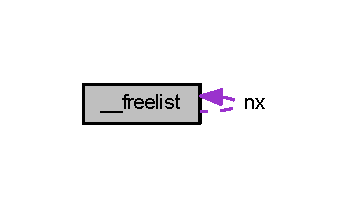
\includegraphics[width=168pt]{struct____freelist__coll__graph}
\end{center}
\end{figure}
\subsection*{Data Fields}
\begin{DoxyCompactItemize}
\item 
size\+\_\+t \hyperlink{struct____freelist_aad50db3bff52eed270f16ef9e6acd8b1}{sz}
\item 
struct \hyperlink{struct____freelist}{\+\_\+\+\_\+freelist} $\ast$ \hyperlink{struct____freelist_ae718f53598ce7902b5c21759e2d0a2ec}{nx}
\end{DoxyCompactItemize}


\subsection{Detailed Description}


Definition at line 38 of file stdlib\+\_\+private.\+h.



\subsection{Field Documentation}
\hypertarget{struct____freelist_ae718f53598ce7902b5c21759e2d0a2ec}{}\index{\+\_\+\+\_\+freelist@{\+\_\+\+\_\+freelist}!nx@{nx}}
\index{nx@{nx}!\+\_\+\+\_\+freelist@{\+\_\+\+\_\+freelist}}
\subsubsection[{nx}]{\setlength{\rightskip}{0pt plus 5cm}struct {\bf \+\_\+\+\_\+freelist}$\ast$ nx}\label{struct____freelist_ae718f53598ce7902b5c21759e2d0a2ec}


Definition at line 40 of file stdlib\+\_\+private.\+h.

\hypertarget{struct____freelist_aad50db3bff52eed270f16ef9e6acd8b1}{}\index{\+\_\+\+\_\+freelist@{\+\_\+\+\_\+freelist}!sz@{sz}}
\index{sz@{sz}!\+\_\+\+\_\+freelist@{\+\_\+\+\_\+freelist}}
\subsubsection[{sz}]{\setlength{\rightskip}{0pt plus 5cm}size\+\_\+t sz}\label{struct____freelist_aad50db3bff52eed270f16ef9e6acd8b1}


Definition at line 39 of file stdlib\+\_\+private.\+h.



The documentation for this struct was generated from the following file\+:\begin{DoxyCompactItemize}
\item 
Arduino\+U\+N\+O/src/arduino/cores/arduino/avr-\/libc/\hyperlink{stdlib__private_8h}{stdlib\+\_\+private.\+h}\end{DoxyCompactItemize}

\hypertarget{struct_a_c_m_functional_descriptor}{}\section{A\+C\+M\+Functional\+Descriptor Struct Reference}
\label{struct_a_c_m_functional_descriptor}\index{A\+C\+M\+Functional\+Descriptor@{A\+C\+M\+Functional\+Descriptor}}


{\ttfamily \#include $<$U\+S\+B\+Core.\+h$>$}

\subsection*{Data Fields}
\begin{DoxyCompactItemize}
\item 
\hyperlink{_u_s_b_a_p_i_8h_aed742c436da53c1080638ce6ef7d13de}{u8} \hyperlink{struct_a_c_m_functional_descriptor_afbf3f3230446569534d5f466aaf4c23b}{len}
\item 
\hyperlink{_u_s_b_a_p_i_8h_aed742c436da53c1080638ce6ef7d13de}{u8} \hyperlink{struct_a_c_m_functional_descriptor_a0bb419531ec75697e63e9109fecf81b0}{dtype}
\item 
\hyperlink{_u_s_b_a_p_i_8h_aed742c436da53c1080638ce6ef7d13de}{u8} \hyperlink{struct_a_c_m_functional_descriptor_afb82dd1313bc5284e4e5aef8218ef414}{subtype}
\item 
\hyperlink{_u_s_b_a_p_i_8h_aed742c436da53c1080638ce6ef7d13de}{u8} \hyperlink{struct_a_c_m_functional_descriptor_a9ad7ca27543639baeed1b53c6f24e149}{bm\+Capabilities}
\end{DoxyCompactItemize}


\subsection{Detailed Description}


Definition at line 226 of file U\+S\+B\+Core.\+h.



\subsection{Field Documentation}
\hypertarget{struct_a_c_m_functional_descriptor_a9ad7ca27543639baeed1b53c6f24e149}{}\index{A\+C\+M\+Functional\+Descriptor@{A\+C\+M\+Functional\+Descriptor}!bm\+Capabilities@{bm\+Capabilities}}
\index{bm\+Capabilities@{bm\+Capabilities}!A\+C\+M\+Functional\+Descriptor@{A\+C\+M\+Functional\+Descriptor}}
\subsubsection[{bm\+Capabilities}]{\setlength{\rightskip}{0pt plus 5cm}{\bf u8} bm\+Capabilities}\label{struct_a_c_m_functional_descriptor_a9ad7ca27543639baeed1b53c6f24e149}


Definition at line 231 of file U\+S\+B\+Core.\+h.

\hypertarget{struct_a_c_m_functional_descriptor_a0bb419531ec75697e63e9109fecf81b0}{}\index{A\+C\+M\+Functional\+Descriptor@{A\+C\+M\+Functional\+Descriptor}!dtype@{dtype}}
\index{dtype@{dtype}!A\+C\+M\+Functional\+Descriptor@{A\+C\+M\+Functional\+Descriptor}}
\subsubsection[{dtype}]{\setlength{\rightskip}{0pt plus 5cm}{\bf u8} dtype}\label{struct_a_c_m_functional_descriptor_a0bb419531ec75697e63e9109fecf81b0}


Definition at line 229 of file U\+S\+B\+Core.\+h.

\hypertarget{struct_a_c_m_functional_descriptor_afbf3f3230446569534d5f466aaf4c23b}{}\index{A\+C\+M\+Functional\+Descriptor@{A\+C\+M\+Functional\+Descriptor}!len@{len}}
\index{len@{len}!A\+C\+M\+Functional\+Descriptor@{A\+C\+M\+Functional\+Descriptor}}
\subsubsection[{len}]{\setlength{\rightskip}{0pt plus 5cm}{\bf u8} len}\label{struct_a_c_m_functional_descriptor_afbf3f3230446569534d5f466aaf4c23b}


Definition at line 228 of file U\+S\+B\+Core.\+h.

\hypertarget{struct_a_c_m_functional_descriptor_afb82dd1313bc5284e4e5aef8218ef414}{}\index{A\+C\+M\+Functional\+Descriptor@{A\+C\+M\+Functional\+Descriptor}!subtype@{subtype}}
\index{subtype@{subtype}!A\+C\+M\+Functional\+Descriptor@{A\+C\+M\+Functional\+Descriptor}}
\subsubsection[{subtype}]{\setlength{\rightskip}{0pt plus 5cm}{\bf u8} subtype}\label{struct_a_c_m_functional_descriptor_afb82dd1313bc5284e4e5aef8218ef414}


Definition at line 230 of file U\+S\+B\+Core.\+h.



The documentation for this struct was generated from the following file\+:\begin{DoxyCompactItemize}
\item 
Arduino\+U\+N\+O/src/arduino/cores/arduino/\hyperlink{_u_s_b_core_8h}{U\+S\+B\+Core.\+h}\end{DoxyCompactItemize}

\hypertarget{struct_c_d_c_c_s_interface_descriptor}{}\section{C\+D\+C\+C\+S\+Interface\+Descriptor Struct Reference}
\label{struct_c_d_c_c_s_interface_descriptor}\index{C\+D\+C\+C\+S\+Interface\+Descriptor@{C\+D\+C\+C\+S\+Interface\+Descriptor}}


{\ttfamily \#include $<$U\+S\+B\+Core.\+h$>$}

\subsection*{Data Fields}
\begin{DoxyCompactItemize}
\item 
\hyperlink{_u_s_b_a_p_i_8h_aed742c436da53c1080638ce6ef7d13de}{u8} \hyperlink{struct_c_d_c_c_s_interface_descriptor_afbf3f3230446569534d5f466aaf4c23b}{len}
\item 
\hyperlink{_u_s_b_a_p_i_8h_aed742c436da53c1080638ce6ef7d13de}{u8} \hyperlink{struct_c_d_c_c_s_interface_descriptor_a0bb419531ec75697e63e9109fecf81b0}{dtype}
\item 
\hyperlink{_u_s_b_a_p_i_8h_aed742c436da53c1080638ce6ef7d13de}{u8} \hyperlink{struct_c_d_c_c_s_interface_descriptor_afb82dd1313bc5284e4e5aef8218ef414}{subtype}
\item 
\hyperlink{_u_s_b_a_p_i_8h_aed742c436da53c1080638ce6ef7d13de}{u8} \hyperlink{struct_c_d_c_c_s_interface_descriptor_a3e359aaf0f33f4eeedb3f26e73ac1cc7}{d0}
\item 
\hyperlink{_u_s_b_a_p_i_8h_aed742c436da53c1080638ce6ef7d13de}{u8} \hyperlink{struct_c_d_c_c_s_interface_descriptor_ac1f3ea17c85c96dbc7ec1dba968be24f}{d1}
\end{DoxyCompactItemize}


\subsection{Detailed Description}


Definition at line 200 of file U\+S\+B\+Core.\+h.



\subsection{Field Documentation}
\hypertarget{struct_c_d_c_c_s_interface_descriptor_a3e359aaf0f33f4eeedb3f26e73ac1cc7}{}\index{C\+D\+C\+C\+S\+Interface\+Descriptor@{C\+D\+C\+C\+S\+Interface\+Descriptor}!d0@{d0}}
\index{d0@{d0}!C\+D\+C\+C\+S\+Interface\+Descriptor@{C\+D\+C\+C\+S\+Interface\+Descriptor}}
\subsubsection[{d0}]{\setlength{\rightskip}{0pt plus 5cm}{\bf u8} d0}\label{struct_c_d_c_c_s_interface_descriptor_a3e359aaf0f33f4eeedb3f26e73ac1cc7}


Definition at line 205 of file U\+S\+B\+Core.\+h.

\hypertarget{struct_c_d_c_c_s_interface_descriptor_ac1f3ea17c85c96dbc7ec1dba968be24f}{}\index{C\+D\+C\+C\+S\+Interface\+Descriptor@{C\+D\+C\+C\+S\+Interface\+Descriptor}!d1@{d1}}
\index{d1@{d1}!C\+D\+C\+C\+S\+Interface\+Descriptor@{C\+D\+C\+C\+S\+Interface\+Descriptor}}
\subsubsection[{d1}]{\setlength{\rightskip}{0pt plus 5cm}{\bf u8} d1}\label{struct_c_d_c_c_s_interface_descriptor_ac1f3ea17c85c96dbc7ec1dba968be24f}


Definition at line 206 of file U\+S\+B\+Core.\+h.

\hypertarget{struct_c_d_c_c_s_interface_descriptor_a0bb419531ec75697e63e9109fecf81b0}{}\index{C\+D\+C\+C\+S\+Interface\+Descriptor@{C\+D\+C\+C\+S\+Interface\+Descriptor}!dtype@{dtype}}
\index{dtype@{dtype}!C\+D\+C\+C\+S\+Interface\+Descriptor@{C\+D\+C\+C\+S\+Interface\+Descriptor}}
\subsubsection[{dtype}]{\setlength{\rightskip}{0pt plus 5cm}{\bf u8} dtype}\label{struct_c_d_c_c_s_interface_descriptor_a0bb419531ec75697e63e9109fecf81b0}


Definition at line 203 of file U\+S\+B\+Core.\+h.

\hypertarget{struct_c_d_c_c_s_interface_descriptor_afbf3f3230446569534d5f466aaf4c23b}{}\index{C\+D\+C\+C\+S\+Interface\+Descriptor@{C\+D\+C\+C\+S\+Interface\+Descriptor}!len@{len}}
\index{len@{len}!C\+D\+C\+C\+S\+Interface\+Descriptor@{C\+D\+C\+C\+S\+Interface\+Descriptor}}
\subsubsection[{len}]{\setlength{\rightskip}{0pt plus 5cm}{\bf u8} len}\label{struct_c_d_c_c_s_interface_descriptor_afbf3f3230446569534d5f466aaf4c23b}


Definition at line 202 of file U\+S\+B\+Core.\+h.

\hypertarget{struct_c_d_c_c_s_interface_descriptor_afb82dd1313bc5284e4e5aef8218ef414}{}\index{C\+D\+C\+C\+S\+Interface\+Descriptor@{C\+D\+C\+C\+S\+Interface\+Descriptor}!subtype@{subtype}}
\index{subtype@{subtype}!C\+D\+C\+C\+S\+Interface\+Descriptor@{C\+D\+C\+C\+S\+Interface\+Descriptor}}
\subsubsection[{subtype}]{\setlength{\rightskip}{0pt plus 5cm}{\bf u8} subtype}\label{struct_c_d_c_c_s_interface_descriptor_afb82dd1313bc5284e4e5aef8218ef414}


Definition at line 204 of file U\+S\+B\+Core.\+h.



The documentation for this struct was generated from the following file\+:\begin{DoxyCompactItemize}
\item 
Arduino\+U\+N\+O/src/arduino/cores/arduino/\hyperlink{_u_s_b_core_8h}{U\+S\+B\+Core.\+h}\end{DoxyCompactItemize}

\hypertarget{struct_c_d_c_c_s_interface_descriptor4}{}\section{C\+D\+C\+C\+S\+Interface\+Descriptor4 Struct Reference}
\label{struct_c_d_c_c_s_interface_descriptor4}\index{C\+D\+C\+C\+S\+Interface\+Descriptor4@{C\+D\+C\+C\+S\+Interface\+Descriptor4}}


{\ttfamily \#include $<$U\+S\+B\+Core.\+h$>$}

\subsection*{Data Fields}
\begin{DoxyCompactItemize}
\item 
\hyperlink{_u_s_b_a_p_i_8h_aed742c436da53c1080638ce6ef7d13de}{u8} \hyperlink{struct_c_d_c_c_s_interface_descriptor4_afbf3f3230446569534d5f466aaf4c23b}{len}
\item 
\hyperlink{_u_s_b_a_p_i_8h_aed742c436da53c1080638ce6ef7d13de}{u8} \hyperlink{struct_c_d_c_c_s_interface_descriptor4_a0bb419531ec75697e63e9109fecf81b0}{dtype}
\item 
\hyperlink{_u_s_b_a_p_i_8h_aed742c436da53c1080638ce6ef7d13de}{u8} \hyperlink{struct_c_d_c_c_s_interface_descriptor4_afb82dd1313bc5284e4e5aef8218ef414}{subtype}
\item 
\hyperlink{_u_s_b_a_p_i_8h_aed742c436da53c1080638ce6ef7d13de}{u8} \hyperlink{struct_c_d_c_c_s_interface_descriptor4_a3e359aaf0f33f4eeedb3f26e73ac1cc7}{d0}
\end{DoxyCompactItemize}


\subsection{Detailed Description}


Definition at line 209 of file U\+S\+B\+Core.\+h.



\subsection{Field Documentation}
\hypertarget{struct_c_d_c_c_s_interface_descriptor4_a3e359aaf0f33f4eeedb3f26e73ac1cc7}{}\index{C\+D\+C\+C\+S\+Interface\+Descriptor4@{C\+D\+C\+C\+S\+Interface\+Descriptor4}!d0@{d0}}
\index{d0@{d0}!C\+D\+C\+C\+S\+Interface\+Descriptor4@{C\+D\+C\+C\+S\+Interface\+Descriptor4}}
\subsubsection[{d0}]{\setlength{\rightskip}{0pt plus 5cm}{\bf u8} d0}\label{struct_c_d_c_c_s_interface_descriptor4_a3e359aaf0f33f4eeedb3f26e73ac1cc7}


Definition at line 214 of file U\+S\+B\+Core.\+h.

\hypertarget{struct_c_d_c_c_s_interface_descriptor4_a0bb419531ec75697e63e9109fecf81b0}{}\index{C\+D\+C\+C\+S\+Interface\+Descriptor4@{C\+D\+C\+C\+S\+Interface\+Descriptor4}!dtype@{dtype}}
\index{dtype@{dtype}!C\+D\+C\+C\+S\+Interface\+Descriptor4@{C\+D\+C\+C\+S\+Interface\+Descriptor4}}
\subsubsection[{dtype}]{\setlength{\rightskip}{0pt plus 5cm}{\bf u8} dtype}\label{struct_c_d_c_c_s_interface_descriptor4_a0bb419531ec75697e63e9109fecf81b0}


Definition at line 212 of file U\+S\+B\+Core.\+h.

\hypertarget{struct_c_d_c_c_s_interface_descriptor4_afbf3f3230446569534d5f466aaf4c23b}{}\index{C\+D\+C\+C\+S\+Interface\+Descriptor4@{C\+D\+C\+C\+S\+Interface\+Descriptor4}!len@{len}}
\index{len@{len}!C\+D\+C\+C\+S\+Interface\+Descriptor4@{C\+D\+C\+C\+S\+Interface\+Descriptor4}}
\subsubsection[{len}]{\setlength{\rightskip}{0pt plus 5cm}{\bf u8} len}\label{struct_c_d_c_c_s_interface_descriptor4_afbf3f3230446569534d5f466aaf4c23b}


Definition at line 211 of file U\+S\+B\+Core.\+h.

\hypertarget{struct_c_d_c_c_s_interface_descriptor4_afb82dd1313bc5284e4e5aef8218ef414}{}\index{C\+D\+C\+C\+S\+Interface\+Descriptor4@{C\+D\+C\+C\+S\+Interface\+Descriptor4}!subtype@{subtype}}
\index{subtype@{subtype}!C\+D\+C\+C\+S\+Interface\+Descriptor4@{C\+D\+C\+C\+S\+Interface\+Descriptor4}}
\subsubsection[{subtype}]{\setlength{\rightskip}{0pt plus 5cm}{\bf u8} subtype}\label{struct_c_d_c_c_s_interface_descriptor4_afb82dd1313bc5284e4e5aef8218ef414}


Definition at line 213 of file U\+S\+B\+Core.\+h.



The documentation for this struct was generated from the following file\+:\begin{DoxyCompactItemize}
\item 
Arduino\+U\+N\+O/src/arduino/cores/arduino/\hyperlink{_u_s_b_core_8h}{U\+S\+B\+Core.\+h}\end{DoxyCompactItemize}

\hypertarget{struct_c_d_c_descriptor}{}\section{C\+D\+C\+Descriptor Struct Reference}
\label{struct_c_d_c_descriptor}\index{C\+D\+C\+Descriptor@{C\+D\+C\+Descriptor}}


{\ttfamily \#include $<$U\+S\+B\+Core.\+h$>$}



Collaboration diagram for C\+D\+C\+Descriptor\+:
\nopagebreak
\begin{figure}[H]
\begin{center}
\leavevmode
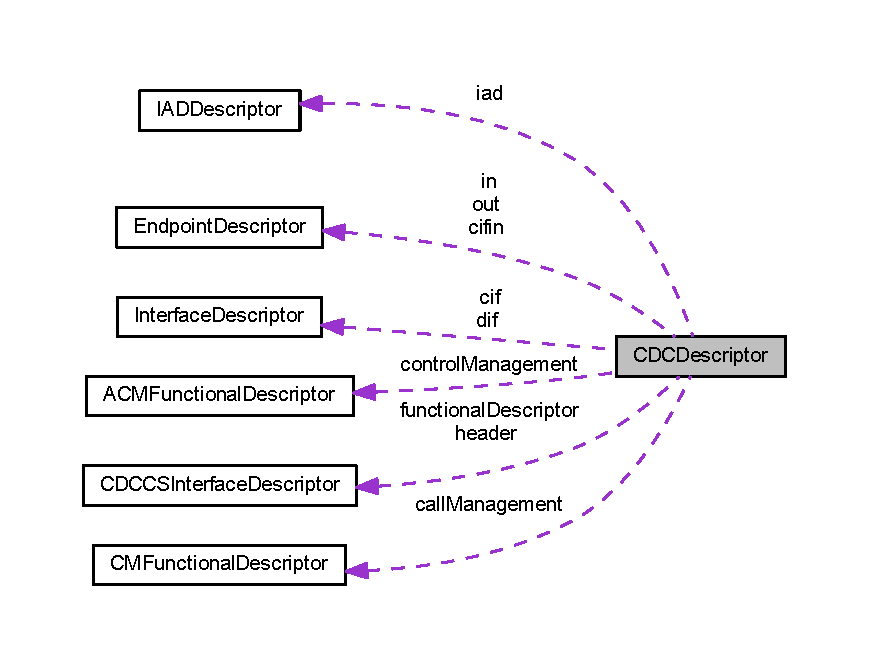
\includegraphics[width=350pt]{struct_c_d_c_descriptor__coll__graph}
\end{center}
\end{figure}
\subsection*{Data Fields}
\begin{DoxyCompactItemize}
\item 
\hyperlink{struct_i_a_d_descriptor}{I\+A\+D\+Descriptor} \hyperlink{struct_c_d_c_descriptor_a934c0c9afb655c1127dc081488de0952}{iad}
\item 
\hyperlink{struct_interface_descriptor}{Interface\+Descriptor} \hyperlink{struct_c_d_c_descriptor_a59ca319c155277d02e33d59292dc6d42}{cif}
\item 
\hyperlink{struct_c_d_c_c_s_interface_descriptor}{C\+D\+C\+C\+S\+Interface\+Descriptor} \hyperlink{struct_c_d_c_descriptor_a8cb2af4efd1b36ad3d11f1176a5628b3}{header}
\item 
\hyperlink{struct_c_m_functional_descriptor}{C\+M\+Functional\+Descriptor} \hyperlink{struct_c_d_c_descriptor_a72f10e0be1c5b49a3bbd81111053bf3e}{call\+Management}
\item 
\hyperlink{struct_a_c_m_functional_descriptor}{A\+C\+M\+Functional\+Descriptor} \hyperlink{struct_c_d_c_descriptor_af1f3192e4a02d190879896f1a664e8b3}{control\+Management}
\item 
\hyperlink{struct_c_d_c_c_s_interface_descriptor}{C\+D\+C\+C\+S\+Interface\+Descriptor} \hyperlink{struct_c_d_c_descriptor_a94d8e9fea32078b996a9e272e1904c07}{functional\+Descriptor}
\item 
\hyperlink{struct_endpoint_descriptor}{Endpoint\+Descriptor} \hyperlink{struct_c_d_c_descriptor_aceee3836101f5463719c5d4bfb8cecd7}{cifin}
\item 
\hyperlink{struct_interface_descriptor}{Interface\+Descriptor} \hyperlink{struct_c_d_c_descriptor_a631454a199b3c6c9ff9764fbe1b19568}{dif}
\item 
\hyperlink{struct_endpoint_descriptor}{Endpoint\+Descriptor} \hyperlink{struct_c_d_c_descriptor_a93dcef3b3e3062b904269bcad94771b5}{in}
\item 
\hyperlink{struct_endpoint_descriptor}{Endpoint\+Descriptor} \hyperlink{struct_c_d_c_descriptor_afcf3c947c6e5ace7853bc3e313c0c4aa}{out}
\end{DoxyCompactItemize}


\subsection{Detailed Description}


Definition at line 234 of file U\+S\+B\+Core.\+h.



\subsection{Field Documentation}
\hypertarget{struct_c_d_c_descriptor_a72f10e0be1c5b49a3bbd81111053bf3e}{}\index{C\+D\+C\+Descriptor@{C\+D\+C\+Descriptor}!call\+Management@{call\+Management}}
\index{call\+Management@{call\+Management}!C\+D\+C\+Descriptor@{C\+D\+C\+Descriptor}}
\subsubsection[{call\+Management}]{\setlength{\rightskip}{0pt plus 5cm}{\bf C\+M\+Functional\+Descriptor} call\+Management}\label{struct_c_d_c_descriptor_a72f10e0be1c5b49a3bbd81111053bf3e}


Definition at line 242 of file U\+S\+B\+Core.\+h.

\hypertarget{struct_c_d_c_descriptor_a59ca319c155277d02e33d59292dc6d42}{}\index{C\+D\+C\+Descriptor@{C\+D\+C\+Descriptor}!cif@{cif}}
\index{cif@{cif}!C\+D\+C\+Descriptor@{C\+D\+C\+Descriptor}}
\subsubsection[{cif}]{\setlength{\rightskip}{0pt plus 5cm}{\bf Interface\+Descriptor} cif}\label{struct_c_d_c_descriptor_a59ca319c155277d02e33d59292dc6d42}


Definition at line 240 of file U\+S\+B\+Core.\+h.

\hypertarget{struct_c_d_c_descriptor_aceee3836101f5463719c5d4bfb8cecd7}{}\index{C\+D\+C\+Descriptor@{C\+D\+C\+Descriptor}!cifin@{cifin}}
\index{cifin@{cifin}!C\+D\+C\+Descriptor@{C\+D\+C\+Descriptor}}
\subsubsection[{cifin}]{\setlength{\rightskip}{0pt plus 5cm}{\bf Endpoint\+Descriptor} cifin}\label{struct_c_d_c_descriptor_aceee3836101f5463719c5d4bfb8cecd7}


Definition at line 245 of file U\+S\+B\+Core.\+h.

\hypertarget{struct_c_d_c_descriptor_af1f3192e4a02d190879896f1a664e8b3}{}\index{C\+D\+C\+Descriptor@{C\+D\+C\+Descriptor}!control\+Management@{control\+Management}}
\index{control\+Management@{control\+Management}!C\+D\+C\+Descriptor@{C\+D\+C\+Descriptor}}
\subsubsection[{control\+Management}]{\setlength{\rightskip}{0pt plus 5cm}{\bf A\+C\+M\+Functional\+Descriptor} control\+Management}\label{struct_c_d_c_descriptor_af1f3192e4a02d190879896f1a664e8b3}


Definition at line 243 of file U\+S\+B\+Core.\+h.

\hypertarget{struct_c_d_c_descriptor_a631454a199b3c6c9ff9764fbe1b19568}{}\index{C\+D\+C\+Descriptor@{C\+D\+C\+Descriptor}!dif@{dif}}
\index{dif@{dif}!C\+D\+C\+Descriptor@{C\+D\+C\+Descriptor}}
\subsubsection[{dif}]{\setlength{\rightskip}{0pt plus 5cm}{\bf Interface\+Descriptor} dif}\label{struct_c_d_c_descriptor_a631454a199b3c6c9ff9764fbe1b19568}


Definition at line 248 of file U\+S\+B\+Core.\+h.

\hypertarget{struct_c_d_c_descriptor_a94d8e9fea32078b996a9e272e1904c07}{}\index{C\+D\+C\+Descriptor@{C\+D\+C\+Descriptor}!functional\+Descriptor@{functional\+Descriptor}}
\index{functional\+Descriptor@{functional\+Descriptor}!C\+D\+C\+Descriptor@{C\+D\+C\+Descriptor}}
\subsubsection[{functional\+Descriptor}]{\setlength{\rightskip}{0pt plus 5cm}{\bf C\+D\+C\+C\+S\+Interface\+Descriptor} functional\+Descriptor}\label{struct_c_d_c_descriptor_a94d8e9fea32078b996a9e272e1904c07}


Definition at line 244 of file U\+S\+B\+Core.\+h.

\hypertarget{struct_c_d_c_descriptor_a8cb2af4efd1b36ad3d11f1176a5628b3}{}\index{C\+D\+C\+Descriptor@{C\+D\+C\+Descriptor}!header@{header}}
\index{header@{header}!C\+D\+C\+Descriptor@{C\+D\+C\+Descriptor}}
\subsubsection[{header}]{\setlength{\rightskip}{0pt plus 5cm}{\bf C\+D\+C\+C\+S\+Interface\+Descriptor} header}\label{struct_c_d_c_descriptor_a8cb2af4efd1b36ad3d11f1176a5628b3}


Definition at line 241 of file U\+S\+B\+Core.\+h.

\hypertarget{struct_c_d_c_descriptor_a934c0c9afb655c1127dc081488de0952}{}\index{C\+D\+C\+Descriptor@{C\+D\+C\+Descriptor}!iad@{iad}}
\index{iad@{iad}!C\+D\+C\+Descriptor@{C\+D\+C\+Descriptor}}
\subsubsection[{iad}]{\setlength{\rightskip}{0pt plus 5cm}{\bf I\+A\+D\+Descriptor} iad}\label{struct_c_d_c_descriptor_a934c0c9afb655c1127dc081488de0952}


Definition at line 237 of file U\+S\+B\+Core.\+h.

\hypertarget{struct_c_d_c_descriptor_a93dcef3b3e3062b904269bcad94771b5}{}\index{C\+D\+C\+Descriptor@{C\+D\+C\+Descriptor}!in@{in}}
\index{in@{in}!C\+D\+C\+Descriptor@{C\+D\+C\+Descriptor}}
\subsubsection[{in}]{\setlength{\rightskip}{0pt plus 5cm}{\bf Endpoint\+Descriptor} in}\label{struct_c_d_c_descriptor_a93dcef3b3e3062b904269bcad94771b5}


Definition at line 249 of file U\+S\+B\+Core.\+h.

\hypertarget{struct_c_d_c_descriptor_afcf3c947c6e5ace7853bc3e313c0c4aa}{}\index{C\+D\+C\+Descriptor@{C\+D\+C\+Descriptor}!out@{out}}
\index{out@{out}!C\+D\+C\+Descriptor@{C\+D\+C\+Descriptor}}
\subsubsection[{out}]{\setlength{\rightskip}{0pt plus 5cm}{\bf Endpoint\+Descriptor} out}\label{struct_c_d_c_descriptor_afcf3c947c6e5ace7853bc3e313c0c4aa}


Definition at line 250 of file U\+S\+B\+Core.\+h.



The documentation for this struct was generated from the following file\+:\begin{DoxyCompactItemize}
\item 
Arduino\+U\+N\+O/src/arduino/cores/arduino/\hyperlink{_u_s_b_core_8h}{U\+S\+B\+Core.\+h}\end{DoxyCompactItemize}

\hypertarget{class_client}{}\section{Client Class Reference}
\label{class_client}\index{Client@{Client}}


{\ttfamily \#include $<$Client.\+h$>$}



Inheritance diagram for Client\+:\nopagebreak
\begin{figure}[H]
\begin{center}
\leavevmode
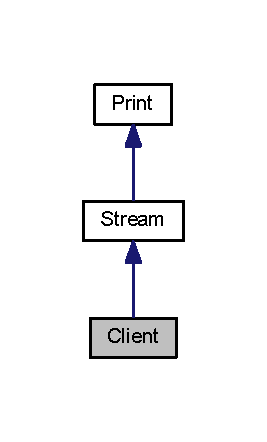
\includegraphics[width=128pt]{class_client__inherit__graph}
\end{center}
\end{figure}


Collaboration diagram for Client\+:\nopagebreak
\begin{figure}[H]
\begin{center}
\leavevmode
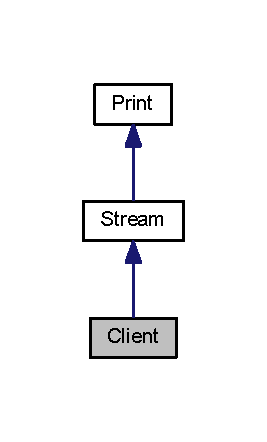
\includegraphics[width=128pt]{class_client__coll__graph}
\end{center}
\end{figure}
\subsection*{Public Member Functions}
\begin{DoxyCompactItemize}
\item 
virtual int \hyperlink{class_client_a7b5d23b2df67ab5f84971100f1f9e825}{connect} (\hyperlink{class_i_p_address}{I\+P\+Address} ip, uint16\+\_\+t port)=0
\item 
virtual int \hyperlink{class_client_a475258d5bda463bac8ac60d391377e34}{connect} (const char $\ast$host, uint16\+\_\+t port)=0
\item 
virtual size\+\_\+t \hyperlink{class_client_acde4db2f92186810af3493fd2c7535f0}{write} (uint8\+\_\+t)=0
\item 
virtual size\+\_\+t \hyperlink{class_client_a7565f7448952b08e42489b3162638f69}{write} (const uint8\+\_\+t $\ast$buf, size\+\_\+t size)=0
\item 
virtual int \hyperlink{class_client_aebd60457902debb30b07971a16f24ebd}{available} ()=0
\item 
virtual int \hyperlink{class_client_a4afd50731ba321d1b9be909cb288a50b}{read} ()=0
\item 
virtual int \hyperlink{class_client_a699f8a687f8e4ab1c08cc4ea1da121bc}{read} (uint8\+\_\+t $\ast$buf, size\+\_\+t size)=0
\item 
virtual int \hyperlink{class_client_a9ae768d427519818aa552adf467bf65a}{peek} ()=0
\item 
virtual void \hyperlink{class_client_a50ab71f4bc571f6e246b20db4b3dd131}{flush} ()=0
\item 
virtual void \hyperlink{class_client_a0efff8623a2fb79dad94a96dcf16d966}{stop} ()=0
\item 
virtual uint8\+\_\+t \hyperlink{class_client_a4da62bf6f27e3c10bc4f7b2d92dca244}{connected} ()=0
\item 
virtual \hyperlink{class_client_ac496133545cba767b45c6ce8df3587e7}{operator bool} ()=0
\end{DoxyCompactItemize}
\subsection*{Protected Member Functions}
\begin{DoxyCompactItemize}
\item 
uint8\+\_\+t $\ast$ \hyperlink{class_client_a8a60fab7dbb23ddc33ffa5163daa52b5}{raw\+I\+P\+Address} (\hyperlink{class_i_p_address}{I\+P\+Address} \&addr)
\end{DoxyCompactItemize}
\subsection*{Additional Inherited Members}


\subsection{Detailed Description}


Definition at line 26 of file Client.\+h.



\subsection{Member Function Documentation}
\hypertarget{class_client_aebd60457902debb30b07971a16f24ebd}{}\index{Client@{Client}!available@{available}}
\index{available@{available}!Client@{Client}}
\subsubsection[{available()=0}]{\setlength{\rightskip}{0pt plus 5cm}virtual int available (
\begin{DoxyParamCaption}
{}
\end{DoxyParamCaption}
)\hspace{0.3cm}{\ttfamily [pure virtual]}}\label{class_client_aebd60457902debb30b07971a16f24ebd}


Implements \hyperlink{class_stream_aebd60457902debb30b07971a16f24ebd}{Stream}.

\hypertarget{class_client_a7b5d23b2df67ab5f84971100f1f9e825}{}\index{Client@{Client}!connect@{connect}}
\index{connect@{connect}!Client@{Client}}
\subsubsection[{connect(\+I\+P\+Address ip, uint16\+\_\+t port)=0}]{\setlength{\rightskip}{0pt plus 5cm}virtual int connect (
\begin{DoxyParamCaption}
\item[{{\bf I\+P\+Address}}]{ip, }
\item[{uint16\+\_\+t}]{port}
\end{DoxyParamCaption}
)\hspace{0.3cm}{\ttfamily [pure virtual]}}\label{class_client_a7b5d23b2df67ab5f84971100f1f9e825}
\hypertarget{class_client_a475258d5bda463bac8ac60d391377e34}{}\index{Client@{Client}!connect@{connect}}
\index{connect@{connect}!Client@{Client}}
\subsubsection[{connect(const char $\ast$host, uint16\+\_\+t port)=0}]{\setlength{\rightskip}{0pt plus 5cm}virtual int connect (
\begin{DoxyParamCaption}
\item[{const char $\ast$}]{host, }
\item[{uint16\+\_\+t}]{port}
\end{DoxyParamCaption}
)\hspace{0.3cm}{\ttfamily [pure virtual]}}\label{class_client_a475258d5bda463bac8ac60d391377e34}
\hypertarget{class_client_a4da62bf6f27e3c10bc4f7b2d92dca244}{}\index{Client@{Client}!connected@{connected}}
\index{connected@{connected}!Client@{Client}}
\subsubsection[{connected()=0}]{\setlength{\rightskip}{0pt plus 5cm}virtual uint8\+\_\+t connected (
\begin{DoxyParamCaption}
{}
\end{DoxyParamCaption}
)\hspace{0.3cm}{\ttfamily [pure virtual]}}\label{class_client_a4da62bf6f27e3c10bc4f7b2d92dca244}
\hypertarget{class_client_a50ab71f4bc571f6e246b20db4b3dd131}{}\index{Client@{Client}!flush@{flush}}
\index{flush@{flush}!Client@{Client}}
\subsubsection[{flush()=0}]{\setlength{\rightskip}{0pt plus 5cm}virtual void flush (
\begin{DoxyParamCaption}
{}
\end{DoxyParamCaption}
)\hspace{0.3cm}{\ttfamily [pure virtual]}}\label{class_client_a50ab71f4bc571f6e246b20db4b3dd131}


Implements \hyperlink{class_stream_a50ab71f4bc571f6e246b20db4b3dd131}{Stream}.

\hypertarget{class_client_ac496133545cba767b45c6ce8df3587e7}{}\index{Client@{Client}!operator bool@{operator bool}}
\index{operator bool@{operator bool}!Client@{Client}}
\subsubsection[{operator bool()=0}]{\setlength{\rightskip}{0pt plus 5cm}virtual operator bool (
\begin{DoxyParamCaption}
{}
\end{DoxyParamCaption}
)\hspace{0.3cm}{\ttfamily [pure virtual]}}\label{class_client_ac496133545cba767b45c6ce8df3587e7}
\hypertarget{class_client_a9ae768d427519818aa552adf467bf65a}{}\index{Client@{Client}!peek@{peek}}
\index{peek@{peek}!Client@{Client}}
\subsubsection[{peek()=0}]{\setlength{\rightskip}{0pt plus 5cm}virtual int peek (
\begin{DoxyParamCaption}
{}
\end{DoxyParamCaption}
)\hspace{0.3cm}{\ttfamily [pure virtual]}}\label{class_client_a9ae768d427519818aa552adf467bf65a}


Implements \hyperlink{class_stream_a9ae768d427519818aa552adf467bf65a}{Stream}.

\hypertarget{class_client_a8a60fab7dbb23ddc33ffa5163daa52b5}{}\index{Client@{Client}!raw\+I\+P\+Address@{raw\+I\+P\+Address}}
\index{raw\+I\+P\+Address@{raw\+I\+P\+Address}!Client@{Client}}
\subsubsection[{raw\+I\+P\+Address(\+I\+P\+Address \&addr)}]{\setlength{\rightskip}{0pt plus 5cm}uint8\+\_\+t$\ast$ raw\+I\+P\+Address (
\begin{DoxyParamCaption}
\item[{{\bf I\+P\+Address} \&}]{addr}
\end{DoxyParamCaption}
)\hspace{0.3cm}{\ttfamily [inline]}, {\ttfamily [protected]}}\label{class_client_a8a60fab7dbb23ddc33ffa5163daa52b5}


Definition at line 42 of file Client.\+h.

\hypertarget{class_client_a4afd50731ba321d1b9be909cb288a50b}{}\index{Client@{Client}!read@{read}}
\index{read@{read}!Client@{Client}}
\subsubsection[{read()=0}]{\setlength{\rightskip}{0pt plus 5cm}virtual int read (
\begin{DoxyParamCaption}
{}
\end{DoxyParamCaption}
)\hspace{0.3cm}{\ttfamily [pure virtual]}}\label{class_client_a4afd50731ba321d1b9be909cb288a50b}


Implements \hyperlink{class_stream_a4afd50731ba321d1b9be909cb288a50b}{Stream}.

\hypertarget{class_client_a699f8a687f8e4ab1c08cc4ea1da121bc}{}\index{Client@{Client}!read@{read}}
\index{read@{read}!Client@{Client}}
\subsubsection[{read(uint8\+\_\+t $\ast$buf, size\+\_\+t size)=0}]{\setlength{\rightskip}{0pt plus 5cm}virtual int read (
\begin{DoxyParamCaption}
\item[{uint8\+\_\+t $\ast$}]{buf, }
\item[{size\+\_\+t}]{size}
\end{DoxyParamCaption}
)\hspace{0.3cm}{\ttfamily [pure virtual]}}\label{class_client_a699f8a687f8e4ab1c08cc4ea1da121bc}
\hypertarget{class_client_a0efff8623a2fb79dad94a96dcf16d966}{}\index{Client@{Client}!stop@{stop}}
\index{stop@{stop}!Client@{Client}}
\subsubsection[{stop()=0}]{\setlength{\rightskip}{0pt plus 5cm}virtual void stop (
\begin{DoxyParamCaption}
{}
\end{DoxyParamCaption}
)\hspace{0.3cm}{\ttfamily [pure virtual]}}\label{class_client_a0efff8623a2fb79dad94a96dcf16d966}
\hypertarget{class_client_acde4db2f92186810af3493fd2c7535f0}{}\index{Client@{Client}!write@{write}}
\index{write@{write}!Client@{Client}}
\subsubsection[{write(uint8\+\_\+t)=0}]{\setlength{\rightskip}{0pt plus 5cm}virtual size\+\_\+t write (
\begin{DoxyParamCaption}
\item[{uint8\+\_\+t}]{}
\end{DoxyParamCaption}
)\hspace{0.3cm}{\ttfamily [pure virtual]}}\label{class_client_acde4db2f92186810af3493fd2c7535f0}


Implements \hyperlink{class_print_acde4db2f92186810af3493fd2c7535f0}{Print}.

\hypertarget{class_client_a7565f7448952b08e42489b3162638f69}{}\index{Client@{Client}!write@{write}}
\index{write@{write}!Client@{Client}}
\subsubsection[{write(const uint8\+\_\+t $\ast$buf, size\+\_\+t size)=0}]{\setlength{\rightskip}{0pt plus 5cm}virtual size\+\_\+t write (
\begin{DoxyParamCaption}
\item[{const uint8\+\_\+t $\ast$}]{buf, }
\item[{size\+\_\+t}]{size}
\end{DoxyParamCaption}
)\hspace{0.3cm}{\ttfamily [pure virtual]}}\label{class_client_a7565f7448952b08e42489b3162638f69}


Reimplemented from \hyperlink{class_print_a7c66fc8d559f4956d4ccea196299bca7}{Print}.



The documentation for this class was generated from the following file\+:\begin{DoxyCompactItemize}
\item 
Arduino\+U\+N\+O/src/arduino/cores/arduino/\hyperlink{_client_8h}{Client.\+h}\end{DoxyCompactItemize}

\hypertarget{struct_c_m_functional_descriptor}{}\section{C\+M\+Functional\+Descriptor Struct Reference}
\label{struct_c_m_functional_descriptor}\index{C\+M\+Functional\+Descriptor@{C\+M\+Functional\+Descriptor}}


{\ttfamily \#include $<$U\+S\+B\+Core.\+h$>$}

\subsection*{Data Fields}
\begin{DoxyCompactItemize}
\item 
\hyperlink{_u_s_b_a_p_i_8h_aed742c436da53c1080638ce6ef7d13de}{u8} \hyperlink{struct_c_m_functional_descriptor_afbf3f3230446569534d5f466aaf4c23b}{len}
\item 
\hyperlink{_u_s_b_a_p_i_8h_aed742c436da53c1080638ce6ef7d13de}{u8} \hyperlink{struct_c_m_functional_descriptor_a0bb419531ec75697e63e9109fecf81b0}{dtype}
\item 
\hyperlink{_u_s_b_a_p_i_8h_aed742c436da53c1080638ce6ef7d13de}{u8} \hyperlink{struct_c_m_functional_descriptor_afb82dd1313bc5284e4e5aef8218ef414}{subtype}
\item 
\hyperlink{_u_s_b_a_p_i_8h_aed742c436da53c1080638ce6ef7d13de}{u8} \hyperlink{struct_c_m_functional_descriptor_a9ad7ca27543639baeed1b53c6f24e149}{bm\+Capabilities}
\item 
\hyperlink{_u_s_b_a_p_i_8h_aed742c436da53c1080638ce6ef7d13de}{u8} \hyperlink{struct_c_m_functional_descriptor_a856be28e5decda9135c9b148a4897716}{b\+Data\+Interface}
\end{DoxyCompactItemize}


\subsection{Detailed Description}


Definition at line 217 of file U\+S\+B\+Core.\+h.



\subsection{Field Documentation}
\hypertarget{struct_c_m_functional_descriptor_a856be28e5decda9135c9b148a4897716}{}\index{C\+M\+Functional\+Descriptor@{C\+M\+Functional\+Descriptor}!b\+Data\+Interface@{b\+Data\+Interface}}
\index{b\+Data\+Interface@{b\+Data\+Interface}!C\+M\+Functional\+Descriptor@{C\+M\+Functional\+Descriptor}}
\subsubsection[{b\+Data\+Interface}]{\setlength{\rightskip}{0pt plus 5cm}{\bf u8} b\+Data\+Interface}\label{struct_c_m_functional_descriptor_a856be28e5decda9135c9b148a4897716}


Definition at line 223 of file U\+S\+B\+Core.\+h.

\hypertarget{struct_c_m_functional_descriptor_a9ad7ca27543639baeed1b53c6f24e149}{}\index{C\+M\+Functional\+Descriptor@{C\+M\+Functional\+Descriptor}!bm\+Capabilities@{bm\+Capabilities}}
\index{bm\+Capabilities@{bm\+Capabilities}!C\+M\+Functional\+Descriptor@{C\+M\+Functional\+Descriptor}}
\subsubsection[{bm\+Capabilities}]{\setlength{\rightskip}{0pt plus 5cm}{\bf u8} bm\+Capabilities}\label{struct_c_m_functional_descriptor_a9ad7ca27543639baeed1b53c6f24e149}


Definition at line 222 of file U\+S\+B\+Core.\+h.

\hypertarget{struct_c_m_functional_descriptor_a0bb419531ec75697e63e9109fecf81b0}{}\index{C\+M\+Functional\+Descriptor@{C\+M\+Functional\+Descriptor}!dtype@{dtype}}
\index{dtype@{dtype}!C\+M\+Functional\+Descriptor@{C\+M\+Functional\+Descriptor}}
\subsubsection[{dtype}]{\setlength{\rightskip}{0pt plus 5cm}{\bf u8} dtype}\label{struct_c_m_functional_descriptor_a0bb419531ec75697e63e9109fecf81b0}


Definition at line 220 of file U\+S\+B\+Core.\+h.

\hypertarget{struct_c_m_functional_descriptor_afbf3f3230446569534d5f466aaf4c23b}{}\index{C\+M\+Functional\+Descriptor@{C\+M\+Functional\+Descriptor}!len@{len}}
\index{len@{len}!C\+M\+Functional\+Descriptor@{C\+M\+Functional\+Descriptor}}
\subsubsection[{len}]{\setlength{\rightskip}{0pt plus 5cm}{\bf u8} len}\label{struct_c_m_functional_descriptor_afbf3f3230446569534d5f466aaf4c23b}


Definition at line 219 of file U\+S\+B\+Core.\+h.

\hypertarget{struct_c_m_functional_descriptor_afb82dd1313bc5284e4e5aef8218ef414}{}\index{C\+M\+Functional\+Descriptor@{C\+M\+Functional\+Descriptor}!subtype@{subtype}}
\index{subtype@{subtype}!C\+M\+Functional\+Descriptor@{C\+M\+Functional\+Descriptor}}
\subsubsection[{subtype}]{\setlength{\rightskip}{0pt plus 5cm}{\bf u8} subtype}\label{struct_c_m_functional_descriptor_afb82dd1313bc5284e4e5aef8218ef414}


Definition at line 221 of file U\+S\+B\+Core.\+h.



The documentation for this struct was generated from the following file\+:\begin{DoxyCompactItemize}
\item 
Arduino\+U\+N\+O/src/arduino/cores/arduino/\hyperlink{_u_s_b_core_8h}{U\+S\+B\+Core.\+h}\end{DoxyCompactItemize}

\hypertarget{struct_config_descriptor}{}\section{Config\+Descriptor Struct Reference}
\label{struct_config_descriptor}\index{Config\+Descriptor@{Config\+Descriptor}}


{\ttfamily \#include $<$U\+S\+B\+Core.\+h$>$}

\subsection*{Data Fields}
\begin{DoxyCompactItemize}
\item 
\hyperlink{_u_s_b_a_p_i_8h_aed742c436da53c1080638ce6ef7d13de}{u8} \hyperlink{struct_config_descriptor_afbf3f3230446569534d5f466aaf4c23b}{len}
\item 
\hyperlink{_u_s_b_a_p_i_8h_aed742c436da53c1080638ce6ef7d13de}{u8} \hyperlink{struct_config_descriptor_a0bb419531ec75697e63e9109fecf81b0}{dtype}
\item 
\hyperlink{_u_s_b_a_p_i_8h_a9e6c91d77e24643b888dbd1a1a590054}{u16} \hyperlink{struct_config_descriptor_aa5da249d1d5f0d5206337b967ca02fc1}{clen}
\item 
\hyperlink{_u_s_b_a_p_i_8h_aed742c436da53c1080638ce6ef7d13de}{u8} \hyperlink{struct_config_descriptor_a14f358f5820bd4d472a16cbe4ca8cee9}{num\+Interfaces}
\item 
\hyperlink{_u_s_b_a_p_i_8h_aed742c436da53c1080638ce6ef7d13de}{u8} \hyperlink{struct_config_descriptor_afbc86c343de9cddaf950200827a9bceb}{config}
\item 
\hyperlink{_u_s_b_a_p_i_8h_aed742c436da53c1080638ce6ef7d13de}{u8} \hyperlink{struct_config_descriptor_aa15641f1c55e92825e8ba97b1dc504a1}{iconfig}
\item 
\hyperlink{_u_s_b_a_p_i_8h_aed742c436da53c1080638ce6ef7d13de}{u8} \hyperlink{struct_config_descriptor_a11c20ff21a3a4209dce65e2d537374bd}{attributes}
\item 
\hyperlink{_u_s_b_a_p_i_8h_aed742c436da53c1080638ce6ef7d13de}{u8} \hyperlink{struct_config_descriptor_a081afc2b5fe7d7e625c612cc09b17015}{max\+Power}
\end{DoxyCompactItemize}


\subsection{Detailed Description}


Definition at line 147 of file U\+S\+B\+Core.\+h.



\subsection{Field Documentation}
\hypertarget{struct_config_descriptor_a11c20ff21a3a4209dce65e2d537374bd}{}\index{Config\+Descriptor@{Config\+Descriptor}!attributes@{attributes}}
\index{attributes@{attributes}!Config\+Descriptor@{Config\+Descriptor}}
\subsubsection[{attributes}]{\setlength{\rightskip}{0pt plus 5cm}{\bf u8} attributes}\label{struct_config_descriptor_a11c20ff21a3a4209dce65e2d537374bd}


Definition at line 154 of file U\+S\+B\+Core.\+h.

\hypertarget{struct_config_descriptor_aa5da249d1d5f0d5206337b967ca02fc1}{}\index{Config\+Descriptor@{Config\+Descriptor}!clen@{clen}}
\index{clen@{clen}!Config\+Descriptor@{Config\+Descriptor}}
\subsubsection[{clen}]{\setlength{\rightskip}{0pt plus 5cm}{\bf u16} clen}\label{struct_config_descriptor_aa5da249d1d5f0d5206337b967ca02fc1}


Definition at line 150 of file U\+S\+B\+Core.\+h.

\hypertarget{struct_config_descriptor_afbc86c343de9cddaf950200827a9bceb}{}\index{Config\+Descriptor@{Config\+Descriptor}!config@{config}}
\index{config@{config}!Config\+Descriptor@{Config\+Descriptor}}
\subsubsection[{config}]{\setlength{\rightskip}{0pt plus 5cm}{\bf u8} config}\label{struct_config_descriptor_afbc86c343de9cddaf950200827a9bceb}


Definition at line 152 of file U\+S\+B\+Core.\+h.

\hypertarget{struct_config_descriptor_a0bb419531ec75697e63e9109fecf81b0}{}\index{Config\+Descriptor@{Config\+Descriptor}!dtype@{dtype}}
\index{dtype@{dtype}!Config\+Descriptor@{Config\+Descriptor}}
\subsubsection[{dtype}]{\setlength{\rightskip}{0pt plus 5cm}{\bf u8} dtype}\label{struct_config_descriptor_a0bb419531ec75697e63e9109fecf81b0}


Definition at line 149 of file U\+S\+B\+Core.\+h.

\hypertarget{struct_config_descriptor_aa15641f1c55e92825e8ba97b1dc504a1}{}\index{Config\+Descriptor@{Config\+Descriptor}!iconfig@{iconfig}}
\index{iconfig@{iconfig}!Config\+Descriptor@{Config\+Descriptor}}
\subsubsection[{iconfig}]{\setlength{\rightskip}{0pt plus 5cm}{\bf u8} iconfig}\label{struct_config_descriptor_aa15641f1c55e92825e8ba97b1dc504a1}


Definition at line 153 of file U\+S\+B\+Core.\+h.

\hypertarget{struct_config_descriptor_afbf3f3230446569534d5f466aaf4c23b}{}\index{Config\+Descriptor@{Config\+Descriptor}!len@{len}}
\index{len@{len}!Config\+Descriptor@{Config\+Descriptor}}
\subsubsection[{len}]{\setlength{\rightskip}{0pt plus 5cm}{\bf u8} len}\label{struct_config_descriptor_afbf3f3230446569534d5f466aaf4c23b}


Definition at line 148 of file U\+S\+B\+Core.\+h.

\hypertarget{struct_config_descriptor_a081afc2b5fe7d7e625c612cc09b17015}{}\index{Config\+Descriptor@{Config\+Descriptor}!max\+Power@{max\+Power}}
\index{max\+Power@{max\+Power}!Config\+Descriptor@{Config\+Descriptor}}
\subsubsection[{max\+Power}]{\setlength{\rightskip}{0pt plus 5cm}{\bf u8} max\+Power}\label{struct_config_descriptor_a081afc2b5fe7d7e625c612cc09b17015}


Definition at line 155 of file U\+S\+B\+Core.\+h.

\hypertarget{struct_config_descriptor_a14f358f5820bd4d472a16cbe4ca8cee9}{}\index{Config\+Descriptor@{Config\+Descriptor}!num\+Interfaces@{num\+Interfaces}}
\index{num\+Interfaces@{num\+Interfaces}!Config\+Descriptor@{Config\+Descriptor}}
\subsubsection[{num\+Interfaces}]{\setlength{\rightskip}{0pt plus 5cm}{\bf u8} num\+Interfaces}\label{struct_config_descriptor_a14f358f5820bd4d472a16cbe4ca8cee9}


Definition at line 151 of file U\+S\+B\+Core.\+h.



The documentation for this struct was generated from the following file\+:\begin{DoxyCompactItemize}
\item 
Arduino\+U\+N\+O/src/arduino/cores/arduino/\hyperlink{_u_s_b_core_8h}{U\+S\+B\+Core.\+h}\end{DoxyCompactItemize}

\hypertarget{struct_device_descriptor}{}\section{Device\+Descriptor Struct Reference}
\label{struct_device_descriptor}\index{Device\+Descriptor@{Device\+Descriptor}}


{\ttfamily \#include $<$U\+S\+B\+Core.\+h$>$}

\subsection*{Data Fields}
\begin{DoxyCompactItemize}
\item 
\hyperlink{_u_s_b_a_p_i_8h_aed742c436da53c1080638ce6ef7d13de}{u8} \hyperlink{struct_device_descriptor_afbf3f3230446569534d5f466aaf4c23b}{len}
\item 
\hyperlink{_u_s_b_a_p_i_8h_aed742c436da53c1080638ce6ef7d13de}{u8} \hyperlink{struct_device_descriptor_a0bb419531ec75697e63e9109fecf81b0}{dtype}
\item 
\hyperlink{_u_s_b_a_p_i_8h_a9e6c91d77e24643b888dbd1a1a590054}{u16} \hyperlink{struct_device_descriptor_a0d9dca86e0ffcd6d89828e4b8b0eb8a0}{usb\+Version}
\item 
\hyperlink{_u_s_b_a_p_i_8h_aed742c436da53c1080638ce6ef7d13de}{u8} \hyperlink{struct_device_descriptor_ac951c25b0d755d42cb5f4a13692d511c}{device\+Class}
\item 
\hyperlink{_u_s_b_a_p_i_8h_aed742c436da53c1080638ce6ef7d13de}{u8} \hyperlink{struct_device_descriptor_a243c174d359ded5ed54cf06d979cab2a}{device\+Sub\+Class}
\item 
\hyperlink{_u_s_b_a_p_i_8h_aed742c436da53c1080638ce6ef7d13de}{u8} \hyperlink{struct_device_descriptor_a1fd727fcfe6f95b1da93b158569777dd}{device\+Protocol}
\item 
\hyperlink{_u_s_b_a_p_i_8h_aed742c436da53c1080638ce6ef7d13de}{u8} \hyperlink{struct_device_descriptor_a8ccac084f7a6348f5719d6081fcc044e}{packet\+Size0}
\item 
\hyperlink{_u_s_b_a_p_i_8h_a9e6c91d77e24643b888dbd1a1a590054}{u16} \hyperlink{struct_device_descriptor_a7a7c71d161c32f997811107e4d546ca8}{id\+Vendor}
\item 
\hyperlink{_u_s_b_a_p_i_8h_a9e6c91d77e24643b888dbd1a1a590054}{u16} \hyperlink{struct_device_descriptor_a519c2f3b9ade6de6e761b4ada00d31b9}{id\+Product}
\item 
\hyperlink{_u_s_b_a_p_i_8h_a9e6c91d77e24643b888dbd1a1a590054}{u16} \hyperlink{struct_device_descriptor_a780fae31c7a1fa955206f55f2a069f02}{device\+Version}
\item 
\hyperlink{_u_s_b_a_p_i_8h_aed742c436da53c1080638ce6ef7d13de}{u8} \hyperlink{struct_device_descriptor_aae88465cfdcbe8c3654a5d317ca2a428}{i\+Manufacturer}
\item 
\hyperlink{_u_s_b_a_p_i_8h_aed742c436da53c1080638ce6ef7d13de}{u8} \hyperlink{struct_device_descriptor_a038aa24fddd7b42b20976e13392954f2}{i\+Product}
\item 
\hyperlink{_u_s_b_a_p_i_8h_aed742c436da53c1080638ce6ef7d13de}{u8} \hyperlink{struct_device_descriptor_ad5cf25949929f3baddc6f1b2751835dc}{i\+Serial\+Number}
\item 
\hyperlink{_u_s_b_a_p_i_8h_aed742c436da53c1080638ce6ef7d13de}{u8} \hyperlink{struct_device_descriptor_a26db168b352c51f781975b270ee76692}{b\+Num\+Configurations}
\end{DoxyCompactItemize}


\subsection{Detailed Description}


Definition at line 129 of file U\+S\+B\+Core.\+h.



\subsection{Field Documentation}
\hypertarget{struct_device_descriptor_a26db168b352c51f781975b270ee76692}{}\index{Device\+Descriptor@{Device\+Descriptor}!b\+Num\+Configurations@{b\+Num\+Configurations}}
\index{b\+Num\+Configurations@{b\+Num\+Configurations}!Device\+Descriptor@{Device\+Descriptor}}
\subsubsection[{b\+Num\+Configurations}]{\setlength{\rightskip}{0pt plus 5cm}{\bf u8} b\+Num\+Configurations}\label{struct_device_descriptor_a26db168b352c51f781975b270ee76692}


Definition at line 143 of file U\+S\+B\+Core.\+h.

\hypertarget{struct_device_descriptor_ac951c25b0d755d42cb5f4a13692d511c}{}\index{Device\+Descriptor@{Device\+Descriptor}!device\+Class@{device\+Class}}
\index{device\+Class@{device\+Class}!Device\+Descriptor@{Device\+Descriptor}}
\subsubsection[{device\+Class}]{\setlength{\rightskip}{0pt plus 5cm}{\bf u8} device\+Class}\label{struct_device_descriptor_ac951c25b0d755d42cb5f4a13692d511c}


Definition at line 133 of file U\+S\+B\+Core.\+h.

\hypertarget{struct_device_descriptor_a1fd727fcfe6f95b1da93b158569777dd}{}\index{Device\+Descriptor@{Device\+Descriptor}!device\+Protocol@{device\+Protocol}}
\index{device\+Protocol@{device\+Protocol}!Device\+Descriptor@{Device\+Descriptor}}
\subsubsection[{device\+Protocol}]{\setlength{\rightskip}{0pt plus 5cm}{\bf u8} device\+Protocol}\label{struct_device_descriptor_a1fd727fcfe6f95b1da93b158569777dd}


Definition at line 135 of file U\+S\+B\+Core.\+h.

\hypertarget{struct_device_descriptor_a243c174d359ded5ed54cf06d979cab2a}{}\index{Device\+Descriptor@{Device\+Descriptor}!device\+Sub\+Class@{device\+Sub\+Class}}
\index{device\+Sub\+Class@{device\+Sub\+Class}!Device\+Descriptor@{Device\+Descriptor}}
\subsubsection[{device\+Sub\+Class}]{\setlength{\rightskip}{0pt plus 5cm}{\bf u8} device\+Sub\+Class}\label{struct_device_descriptor_a243c174d359ded5ed54cf06d979cab2a}


Definition at line 134 of file U\+S\+B\+Core.\+h.

\hypertarget{struct_device_descriptor_a780fae31c7a1fa955206f55f2a069f02}{}\index{Device\+Descriptor@{Device\+Descriptor}!device\+Version@{device\+Version}}
\index{device\+Version@{device\+Version}!Device\+Descriptor@{Device\+Descriptor}}
\subsubsection[{device\+Version}]{\setlength{\rightskip}{0pt plus 5cm}{\bf u16} device\+Version}\label{struct_device_descriptor_a780fae31c7a1fa955206f55f2a069f02}


Definition at line 139 of file U\+S\+B\+Core.\+h.

\hypertarget{struct_device_descriptor_a0bb419531ec75697e63e9109fecf81b0}{}\index{Device\+Descriptor@{Device\+Descriptor}!dtype@{dtype}}
\index{dtype@{dtype}!Device\+Descriptor@{Device\+Descriptor}}
\subsubsection[{dtype}]{\setlength{\rightskip}{0pt plus 5cm}{\bf u8} dtype}\label{struct_device_descriptor_a0bb419531ec75697e63e9109fecf81b0}


Definition at line 131 of file U\+S\+B\+Core.\+h.

\hypertarget{struct_device_descriptor_a519c2f3b9ade6de6e761b4ada00d31b9}{}\index{Device\+Descriptor@{Device\+Descriptor}!id\+Product@{id\+Product}}
\index{id\+Product@{id\+Product}!Device\+Descriptor@{Device\+Descriptor}}
\subsubsection[{id\+Product}]{\setlength{\rightskip}{0pt plus 5cm}{\bf u16} id\+Product}\label{struct_device_descriptor_a519c2f3b9ade6de6e761b4ada00d31b9}


Definition at line 138 of file U\+S\+B\+Core.\+h.

\hypertarget{struct_device_descriptor_a7a7c71d161c32f997811107e4d546ca8}{}\index{Device\+Descriptor@{Device\+Descriptor}!id\+Vendor@{id\+Vendor}}
\index{id\+Vendor@{id\+Vendor}!Device\+Descriptor@{Device\+Descriptor}}
\subsubsection[{id\+Vendor}]{\setlength{\rightskip}{0pt plus 5cm}{\bf u16} id\+Vendor}\label{struct_device_descriptor_a7a7c71d161c32f997811107e4d546ca8}


Definition at line 137 of file U\+S\+B\+Core.\+h.

\hypertarget{struct_device_descriptor_aae88465cfdcbe8c3654a5d317ca2a428}{}\index{Device\+Descriptor@{Device\+Descriptor}!i\+Manufacturer@{i\+Manufacturer}}
\index{i\+Manufacturer@{i\+Manufacturer}!Device\+Descriptor@{Device\+Descriptor}}
\subsubsection[{i\+Manufacturer}]{\setlength{\rightskip}{0pt plus 5cm}{\bf u8} i\+Manufacturer}\label{struct_device_descriptor_aae88465cfdcbe8c3654a5d317ca2a428}


Definition at line 140 of file U\+S\+B\+Core.\+h.

\hypertarget{struct_device_descriptor_a038aa24fddd7b42b20976e13392954f2}{}\index{Device\+Descriptor@{Device\+Descriptor}!i\+Product@{i\+Product}}
\index{i\+Product@{i\+Product}!Device\+Descriptor@{Device\+Descriptor}}
\subsubsection[{i\+Product}]{\setlength{\rightskip}{0pt plus 5cm}{\bf u8} i\+Product}\label{struct_device_descriptor_a038aa24fddd7b42b20976e13392954f2}


Definition at line 141 of file U\+S\+B\+Core.\+h.

\hypertarget{struct_device_descriptor_ad5cf25949929f3baddc6f1b2751835dc}{}\index{Device\+Descriptor@{Device\+Descriptor}!i\+Serial\+Number@{i\+Serial\+Number}}
\index{i\+Serial\+Number@{i\+Serial\+Number}!Device\+Descriptor@{Device\+Descriptor}}
\subsubsection[{i\+Serial\+Number}]{\setlength{\rightskip}{0pt plus 5cm}{\bf u8} i\+Serial\+Number}\label{struct_device_descriptor_ad5cf25949929f3baddc6f1b2751835dc}


Definition at line 142 of file U\+S\+B\+Core.\+h.

\hypertarget{struct_device_descriptor_afbf3f3230446569534d5f466aaf4c23b}{}\index{Device\+Descriptor@{Device\+Descriptor}!len@{len}}
\index{len@{len}!Device\+Descriptor@{Device\+Descriptor}}
\subsubsection[{len}]{\setlength{\rightskip}{0pt plus 5cm}{\bf u8} len}\label{struct_device_descriptor_afbf3f3230446569534d5f466aaf4c23b}


Definition at line 130 of file U\+S\+B\+Core.\+h.

\hypertarget{struct_device_descriptor_a8ccac084f7a6348f5719d6081fcc044e}{}\index{Device\+Descriptor@{Device\+Descriptor}!packet\+Size0@{packet\+Size0}}
\index{packet\+Size0@{packet\+Size0}!Device\+Descriptor@{Device\+Descriptor}}
\subsubsection[{packet\+Size0}]{\setlength{\rightskip}{0pt plus 5cm}{\bf u8} packet\+Size0}\label{struct_device_descriptor_a8ccac084f7a6348f5719d6081fcc044e}


Definition at line 136 of file U\+S\+B\+Core.\+h.

\hypertarget{struct_device_descriptor_a0d9dca86e0ffcd6d89828e4b8b0eb8a0}{}\index{Device\+Descriptor@{Device\+Descriptor}!usb\+Version@{usb\+Version}}
\index{usb\+Version@{usb\+Version}!Device\+Descriptor@{Device\+Descriptor}}
\subsubsection[{usb\+Version}]{\setlength{\rightskip}{0pt plus 5cm}{\bf u16} usb\+Version}\label{struct_device_descriptor_a0d9dca86e0ffcd6d89828e4b8b0eb8a0}


Definition at line 132 of file U\+S\+B\+Core.\+h.



The documentation for this struct was generated from the following file\+:\begin{DoxyCompactItemize}
\item 
Arduino\+U\+N\+O/src/arduino/cores/arduino/\hyperlink{_u_s_b_core_8h}{U\+S\+B\+Core.\+h}\end{DoxyCompactItemize}

\hypertarget{struct_endpoint_descriptor}{}\section{Endpoint\+Descriptor Struct Reference}
\label{struct_endpoint_descriptor}\index{Endpoint\+Descriptor@{Endpoint\+Descriptor}}


{\ttfamily \#include $<$U\+S\+B\+Core.\+h$>$}

\subsection*{Data Fields}
\begin{DoxyCompactItemize}
\item 
\hyperlink{_u_s_b_a_p_i_8h_aed742c436da53c1080638ce6ef7d13de}{u8} \hyperlink{struct_endpoint_descriptor_afbf3f3230446569534d5f466aaf4c23b}{len}
\item 
\hyperlink{_u_s_b_a_p_i_8h_aed742c436da53c1080638ce6ef7d13de}{u8} \hyperlink{struct_endpoint_descriptor_a0bb419531ec75697e63e9109fecf81b0}{dtype}
\item 
\hyperlink{_u_s_b_a_p_i_8h_aed742c436da53c1080638ce6ef7d13de}{u8} \hyperlink{struct_endpoint_descriptor_a7394c0f7cac587defeae4e84d34fb535}{addr}
\item 
\hyperlink{_u_s_b_a_p_i_8h_aed742c436da53c1080638ce6ef7d13de}{u8} \hyperlink{struct_endpoint_descriptor_a76705b0f72861d4d0bef909f56fb34ec}{attr}
\item 
\hyperlink{_u_s_b_a_p_i_8h_a9e6c91d77e24643b888dbd1a1a590054}{u16} \hyperlink{struct_endpoint_descriptor_a198c21ff91822a72041d63f054615143}{packet\+Size}
\item 
\hyperlink{_u_s_b_a_p_i_8h_aed742c436da53c1080638ce6ef7d13de}{u8} \hyperlink{struct_endpoint_descriptor_a10a5b8a25e61bd366aeabe4da95b2cf2}{interval}
\end{DoxyCompactItemize}


\subsection{Detailed Description}


Definition at line 175 of file U\+S\+B\+Core.\+h.



\subsection{Field Documentation}
\hypertarget{struct_endpoint_descriptor_a7394c0f7cac587defeae4e84d34fb535}{}\index{Endpoint\+Descriptor@{Endpoint\+Descriptor}!addr@{addr}}
\index{addr@{addr}!Endpoint\+Descriptor@{Endpoint\+Descriptor}}
\subsubsection[{addr}]{\setlength{\rightskip}{0pt plus 5cm}{\bf u8} addr}\label{struct_endpoint_descriptor_a7394c0f7cac587defeae4e84d34fb535}


Definition at line 179 of file U\+S\+B\+Core.\+h.

\hypertarget{struct_endpoint_descriptor_a76705b0f72861d4d0bef909f56fb34ec}{}\index{Endpoint\+Descriptor@{Endpoint\+Descriptor}!attr@{attr}}
\index{attr@{attr}!Endpoint\+Descriptor@{Endpoint\+Descriptor}}
\subsubsection[{attr}]{\setlength{\rightskip}{0pt plus 5cm}{\bf u8} attr}\label{struct_endpoint_descriptor_a76705b0f72861d4d0bef909f56fb34ec}


Definition at line 180 of file U\+S\+B\+Core.\+h.

\hypertarget{struct_endpoint_descriptor_a0bb419531ec75697e63e9109fecf81b0}{}\index{Endpoint\+Descriptor@{Endpoint\+Descriptor}!dtype@{dtype}}
\index{dtype@{dtype}!Endpoint\+Descriptor@{Endpoint\+Descriptor}}
\subsubsection[{dtype}]{\setlength{\rightskip}{0pt plus 5cm}{\bf u8} dtype}\label{struct_endpoint_descriptor_a0bb419531ec75697e63e9109fecf81b0}


Definition at line 178 of file U\+S\+B\+Core.\+h.

\hypertarget{struct_endpoint_descriptor_a10a5b8a25e61bd366aeabe4da95b2cf2}{}\index{Endpoint\+Descriptor@{Endpoint\+Descriptor}!interval@{interval}}
\index{interval@{interval}!Endpoint\+Descriptor@{Endpoint\+Descriptor}}
\subsubsection[{interval}]{\setlength{\rightskip}{0pt plus 5cm}{\bf u8} interval}\label{struct_endpoint_descriptor_a10a5b8a25e61bd366aeabe4da95b2cf2}


Definition at line 182 of file U\+S\+B\+Core.\+h.

\hypertarget{struct_endpoint_descriptor_afbf3f3230446569534d5f466aaf4c23b}{}\index{Endpoint\+Descriptor@{Endpoint\+Descriptor}!len@{len}}
\index{len@{len}!Endpoint\+Descriptor@{Endpoint\+Descriptor}}
\subsubsection[{len}]{\setlength{\rightskip}{0pt plus 5cm}{\bf u8} len}\label{struct_endpoint_descriptor_afbf3f3230446569534d5f466aaf4c23b}


Definition at line 177 of file U\+S\+B\+Core.\+h.

\hypertarget{struct_endpoint_descriptor_a198c21ff91822a72041d63f054615143}{}\index{Endpoint\+Descriptor@{Endpoint\+Descriptor}!packet\+Size@{packet\+Size}}
\index{packet\+Size@{packet\+Size}!Endpoint\+Descriptor@{Endpoint\+Descriptor}}
\subsubsection[{packet\+Size}]{\setlength{\rightskip}{0pt plus 5cm}{\bf u16} packet\+Size}\label{struct_endpoint_descriptor_a198c21ff91822a72041d63f054615143}


Definition at line 181 of file U\+S\+B\+Core.\+h.



The documentation for this struct was generated from the following file\+:\begin{DoxyCompactItemize}
\item 
Arduino\+U\+N\+O/src/arduino/cores/arduino/\hyperlink{_u_s_b_core_8h}{U\+S\+B\+Core.\+h}\end{DoxyCompactItemize}

\hypertarget{class_hardware_serial}{}\section{Hardware\+Serial Class Reference}
\label{class_hardware_serial}\index{Hardware\+Serial@{Hardware\+Serial}}


{\ttfamily \#include $<$Hardware\+Serial.\+h$>$}



Inheritance diagram for Hardware\+Serial\+:\nopagebreak
\begin{figure}[H]
\begin{center}
\leavevmode
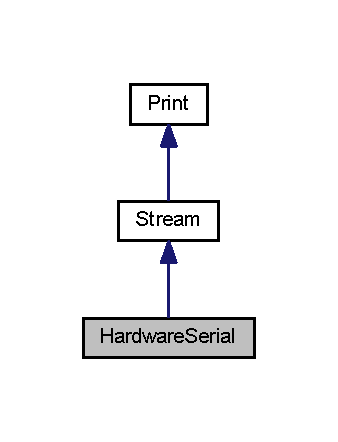
\includegraphics[width=162pt]{class_hardware_serial__inherit__graph}
\end{center}
\end{figure}


Collaboration diagram for Hardware\+Serial\+:\nopagebreak
\begin{figure}[H]
\begin{center}
\leavevmode
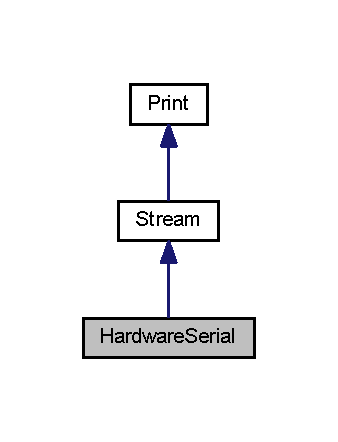
\includegraphics[width=162pt]{class_hardware_serial__coll__graph}
\end{center}
\end{figure}
\subsection*{Public Member Functions}
\begin{DoxyCompactItemize}
\item 
\hyperlink{class_hardware_serial_ab181fe0181fb1fc198b33af34ee13cb4}{Hardware\+Serial} (volatile uint8\+\_\+t $\ast$ubrrh, volatile uint8\+\_\+t $\ast$ubrrl, volatile uint8\+\_\+t $\ast$ucsra, volatile uint8\+\_\+t $\ast$ucsrb, volatile uint8\+\_\+t $\ast$ucsrc, volatile uint8\+\_\+t $\ast$udr)
\item 
void \hyperlink{class_hardware_serial_a384e10dd459783bcba27090520119f3c}{begin} (unsigned long baud)
\item 
void \hyperlink{class_hardware_serial_a6d7cd41eca940345e2ffad77cf08c3bc}{begin} (unsigned long, uint8\+\_\+t)
\item 
void \hyperlink{class_hardware_serial_aaf81d3fdaf258088d7692fa70cece087}{end} ()
\item 
virtual int \hyperlink{class_hardware_serial_aeec8f4dbef97221a6041d6cdc6e9b716}{available} (void)
\item 
virtual int \hyperlink{class_hardware_serial_a65e3a688fcd31f2f486d3af02c400d8f}{peek} (void)
\item 
virtual int \hyperlink{class_hardware_serial_aead319e2866cf90d56c10f2ed39a4396}{read} (void)
\item 
int \hyperlink{class_hardware_serial_a4afe5933dbdb0ad962857d00e04c3bfc}{available\+For\+Write} (void)
\item 
virtual void \hyperlink{class_hardware_serial_a0a4efd3d0f68d057f23eb5dfcd16c17c}{flush} (void)
\item 
virtual size\+\_\+t \hyperlink{class_hardware_serial_a0c15a57daf1517586523b8d270d34c7d}{write} (uint8\+\_\+t)
\item 
size\+\_\+t \hyperlink{class_hardware_serial_a0ba52a995edf9b6c2cdf3d396be84ff1}{write} (unsigned long n)
\item 
size\+\_\+t \hyperlink{class_hardware_serial_a3cfec102ee6f58a2f7e617999ce9f5bb}{write} (long n)
\item 
size\+\_\+t \hyperlink{class_hardware_serial_a2d9bc6ac05e45a7023be3cd1ca224407}{write} (unsigned int n)
\item 
size\+\_\+t \hyperlink{class_hardware_serial_a22e7ab55e0aa268cff5b48e763429ec3}{write} (int n)
\item 
\hyperlink{class_hardware_serial_a9b3baad8c612d81b96e46f84d7e97580}{operator bool} ()
\item 
void \hyperlink{class_hardware_serial_a1e53ef70365848217cf98758e9391ca1}{\+\_\+rx\+\_\+complete\+\_\+irq} (void)
\item 
void \hyperlink{class_hardware_serial_aa3d3b6e82dac8974a0a70c3abf301e70}{\+\_\+tx\+\_\+udr\+\_\+empty\+\_\+irq} (void)
\end{DoxyCompactItemize}
\subsection*{Protected Attributes}
\begin{DoxyCompactItemize}
\item 
volatile uint8\+\_\+t $\ast$const \hyperlink{class_hardware_serial_ac2dd0caa2b74a2992e1b9b0d63dec696}{\+\_\+ubrrh}
\item 
volatile uint8\+\_\+t $\ast$const \hyperlink{class_hardware_serial_ad61fd40f665d597de97ec3995e251e93}{\+\_\+ubrrl}
\item 
volatile uint8\+\_\+t $\ast$const \hyperlink{class_hardware_serial_a691bd409418c1acc6fc583692b54764f}{\+\_\+ucsra}
\item 
volatile uint8\+\_\+t $\ast$const \hyperlink{class_hardware_serial_a06c3d929aa3eb0e48227139d1750a3a7}{\+\_\+ucsrb}
\item 
volatile uint8\+\_\+t $\ast$const \hyperlink{class_hardware_serial_a3599c284453c515776147539d753d1bf}{\+\_\+ucsrc}
\item 
volatile uint8\+\_\+t $\ast$const \hyperlink{class_hardware_serial_a9123daf6c7d2bc8c3997d73f7b30bece}{\+\_\+udr}
\item 
bool \hyperlink{class_hardware_serial_a491255f295202ef6556a978224fdc71e}{\+\_\+written}
\item 
volatile \hyperlink{_hardware_serial_8h_a335e37d0726278844b068d565a4e66b7}{rx\+\_\+buffer\+\_\+index\+\_\+t} \hyperlink{class_hardware_serial_a797ebcc80bc2806b3ebbfc509e7aeabe}{\+\_\+rx\+\_\+buffer\+\_\+head}
\item 
volatile \hyperlink{_hardware_serial_8h_a335e37d0726278844b068d565a4e66b7}{rx\+\_\+buffer\+\_\+index\+\_\+t} \hyperlink{class_hardware_serial_a0343d5d99eb23a56dd3ad5b48928a94a}{\+\_\+rx\+\_\+buffer\+\_\+tail}
\item 
volatile \hyperlink{_hardware_serial_8h_a20cdd352151af0ecef9f3f68c8b20256}{tx\+\_\+buffer\+\_\+index\+\_\+t} \hyperlink{class_hardware_serial_abc7b62797e816bc704bfe3ec80f68607}{\+\_\+tx\+\_\+buffer\+\_\+head}
\item 
volatile \hyperlink{_hardware_serial_8h_a20cdd352151af0ecef9f3f68c8b20256}{tx\+\_\+buffer\+\_\+index\+\_\+t} \hyperlink{class_hardware_serial_a3aad9ccd1bebab9d9226e0c38ee54465}{\+\_\+tx\+\_\+buffer\+\_\+tail}
\item 
unsigned char \hyperlink{class_hardware_serial_ae33d584001d6c3fbbc6a8097b0ab19c7}{\+\_\+rx\+\_\+buffer} \mbox{[}\hyperlink{_hardware_serial_8h_aba0ceec384cf3acb51e0d6f45f31379c}{S\+E\+R\+I\+A\+L\+\_\+\+R\+X\+\_\+\+B\+U\+F\+F\+E\+R\+\_\+\+S\+I\+Z\+E}\mbox{]}
\item 
unsigned char \hyperlink{class_hardware_serial_ae29711a762cbc9a7f622b4f4ff64d374}{\+\_\+tx\+\_\+buffer} \mbox{[}\hyperlink{_hardware_serial_8h_af0d9a9a9aac810bf58f698086f76e516}{S\+E\+R\+I\+A\+L\+\_\+\+T\+X\+\_\+\+B\+U\+F\+F\+E\+R\+\_\+\+S\+I\+Z\+E}\mbox{]}
\end{DoxyCompactItemize}
\subsection*{Additional Inherited Members}


\subsection{Detailed Description}


Definition at line 83 of file Hardware\+Serial.\+h.



\subsection{Constructor \& Destructor Documentation}
\hypertarget{class_hardware_serial_ab181fe0181fb1fc198b33af34ee13cb4}{}\index{Hardware\+Serial@{Hardware\+Serial}!Hardware\+Serial@{Hardware\+Serial}}
\index{Hardware\+Serial@{Hardware\+Serial}!Hardware\+Serial@{Hardware\+Serial}}
\subsubsection[{Hardware\+Serial(volatile uint8\+\_\+t $\ast$ubrrh, volatile uint8\+\_\+t $\ast$ubrrl, volatile uint8\+\_\+t $\ast$ucsra, volatile uint8\+\_\+t $\ast$ucsrb, volatile uint8\+\_\+t $\ast$ucsrc, volatile uint8\+\_\+t $\ast$udr)}]{\setlength{\rightskip}{0pt plus 5cm}{\bf Hardware\+Serial} (
\begin{DoxyParamCaption}
\item[{volatile uint8\+\_\+t $\ast$}]{ubrrh, }
\item[{volatile uint8\+\_\+t $\ast$}]{ubrrl, }
\item[{volatile uint8\+\_\+t $\ast$}]{ucsra, }
\item[{volatile uint8\+\_\+t $\ast$}]{ucsrb, }
\item[{volatile uint8\+\_\+t $\ast$}]{ucsrc, }
\item[{volatile uint8\+\_\+t $\ast$}]{udr}
\end{DoxyParamCaption}
)\hspace{0.3cm}{\ttfamily [inline]}}\label{class_hardware_serial_ab181fe0181fb1fc198b33af34ee13cb4}


\subsection{Member Function Documentation}
\hypertarget{class_hardware_serial_a1e53ef70365848217cf98758e9391ca1}{}\index{Hardware\+Serial@{Hardware\+Serial}!\+\_\+rx\+\_\+complete\+\_\+irq@{\+\_\+rx\+\_\+complete\+\_\+irq}}
\index{\+\_\+rx\+\_\+complete\+\_\+irq@{\+\_\+rx\+\_\+complete\+\_\+irq}!Hardware\+Serial@{Hardware\+Serial}}
\subsubsection[{\+\_\+rx\+\_\+complete\+\_\+irq(void)}]{\setlength{\rightskip}{0pt plus 5cm}void \+\_\+rx\+\_\+complete\+\_\+irq (
\begin{DoxyParamCaption}
\item[{void}]{}
\end{DoxyParamCaption}
)\hspace{0.3cm}{\ttfamily [inline]}}\label{class_hardware_serial_a1e53ef70365848217cf98758e9391ca1}
\hypertarget{class_hardware_serial_aa3d3b6e82dac8974a0a70c3abf301e70}{}\index{Hardware\+Serial@{Hardware\+Serial}!\+\_\+tx\+\_\+udr\+\_\+empty\+\_\+irq@{\+\_\+tx\+\_\+udr\+\_\+empty\+\_\+irq}}
\index{\+\_\+tx\+\_\+udr\+\_\+empty\+\_\+irq@{\+\_\+tx\+\_\+udr\+\_\+empty\+\_\+irq}!Hardware\+Serial@{Hardware\+Serial}}
\subsubsection[{\+\_\+tx\+\_\+udr\+\_\+empty\+\_\+irq(void)}]{\setlength{\rightskip}{0pt plus 5cm}void \+\_\+tx\+\_\+udr\+\_\+empty\+\_\+irq (
\begin{DoxyParamCaption}
\item[{void}]{}
\end{DoxyParamCaption}
)}\label{class_hardware_serial_aa3d3b6e82dac8974a0a70c3abf301e70}
\hypertarget{class_hardware_serial_aeec8f4dbef97221a6041d6cdc6e9b716}{}\index{Hardware\+Serial@{Hardware\+Serial}!available@{available}}
\index{available@{available}!Hardware\+Serial@{Hardware\+Serial}}
\subsubsection[{available(void)}]{\setlength{\rightskip}{0pt plus 5cm}virtual int available (
\begin{DoxyParamCaption}
\item[{void}]{}
\end{DoxyParamCaption}
)\hspace{0.3cm}{\ttfamily [virtual]}}\label{class_hardware_serial_aeec8f4dbef97221a6041d6cdc6e9b716}


Implements \hyperlink{class_stream_aebd60457902debb30b07971a16f24ebd}{Stream}.

\hypertarget{class_hardware_serial_a4afe5933dbdb0ad962857d00e04c3bfc}{}\index{Hardware\+Serial@{Hardware\+Serial}!available\+For\+Write@{available\+For\+Write}}
\index{available\+For\+Write@{available\+For\+Write}!Hardware\+Serial@{Hardware\+Serial}}
\subsubsection[{available\+For\+Write(void)}]{\setlength{\rightskip}{0pt plus 5cm}int available\+For\+Write (
\begin{DoxyParamCaption}
\item[{void}]{}
\end{DoxyParamCaption}
)}\label{class_hardware_serial_a4afe5933dbdb0ad962857d00e04c3bfc}
\hypertarget{class_hardware_serial_a384e10dd459783bcba27090520119f3c}{}\index{Hardware\+Serial@{Hardware\+Serial}!begin@{begin}}
\index{begin@{begin}!Hardware\+Serial@{Hardware\+Serial}}
\subsubsection[{begin(unsigned long baud)}]{\setlength{\rightskip}{0pt plus 5cm}void begin (
\begin{DoxyParamCaption}
\item[{unsigned long}]{baud}
\end{DoxyParamCaption}
)\hspace{0.3cm}{\ttfamily [inline]}}\label{class_hardware_serial_a384e10dd459783bcba27090520119f3c}


Definition at line 111 of file Hardware\+Serial.\+h.



Here is the call graph for this function\+:\nopagebreak
\begin{figure}[H]
\begin{center}
\leavevmode
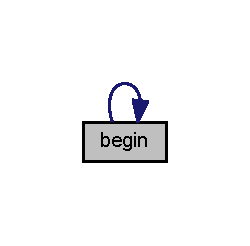
\includegraphics[width=120pt]{class_hardware_serial_a384e10dd459783bcba27090520119f3c_cgraph}
\end{center}
\end{figure}




Here is the caller graph for this function\+:\nopagebreak
\begin{figure}[H]
\begin{center}
\leavevmode
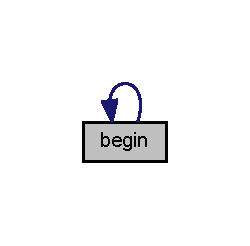
\includegraphics[width=120pt]{class_hardware_serial_a384e10dd459783bcba27090520119f3c_icgraph}
\end{center}
\end{figure}


\hypertarget{class_hardware_serial_a6d7cd41eca940345e2ffad77cf08c3bc}{}\index{Hardware\+Serial@{Hardware\+Serial}!begin@{begin}}
\index{begin@{begin}!Hardware\+Serial@{Hardware\+Serial}}
\subsubsection[{begin(unsigned long, uint8\+\_\+t)}]{\setlength{\rightskip}{0pt plus 5cm}void begin (
\begin{DoxyParamCaption}
\item[{unsigned}]{long, }
\item[{uint8\+\_\+t}]{}
\end{DoxyParamCaption}
)}\label{class_hardware_serial_a6d7cd41eca940345e2ffad77cf08c3bc}
\hypertarget{class_hardware_serial_aaf81d3fdaf258088d7692fa70cece087}{}\index{Hardware\+Serial@{Hardware\+Serial}!end@{end}}
\index{end@{end}!Hardware\+Serial@{Hardware\+Serial}}
\subsubsection[{end()}]{\setlength{\rightskip}{0pt plus 5cm}void end (
\begin{DoxyParamCaption}
{}
\end{DoxyParamCaption}
)}\label{class_hardware_serial_aaf81d3fdaf258088d7692fa70cece087}
\hypertarget{class_hardware_serial_a0a4efd3d0f68d057f23eb5dfcd16c17c}{}\index{Hardware\+Serial@{Hardware\+Serial}!flush@{flush}}
\index{flush@{flush}!Hardware\+Serial@{Hardware\+Serial}}
\subsubsection[{flush(void)}]{\setlength{\rightskip}{0pt plus 5cm}virtual void flush (
\begin{DoxyParamCaption}
\item[{void}]{}
\end{DoxyParamCaption}
)\hspace{0.3cm}{\ttfamily [virtual]}}\label{class_hardware_serial_a0a4efd3d0f68d057f23eb5dfcd16c17c}


Implements \hyperlink{class_stream_a50ab71f4bc571f6e246b20db4b3dd131}{Stream}.

\hypertarget{class_hardware_serial_a9b3baad8c612d81b96e46f84d7e97580}{}\index{Hardware\+Serial@{Hardware\+Serial}!operator bool@{operator bool}}
\index{operator bool@{operator bool}!Hardware\+Serial@{Hardware\+Serial}}
\subsubsection[{operator bool()}]{\setlength{\rightskip}{0pt plus 5cm}operator bool (
\begin{DoxyParamCaption}
{}
\end{DoxyParamCaption}
)\hspace{0.3cm}{\ttfamily [inline]}}\label{class_hardware_serial_a9b3baad8c612d81b96e46f84d7e97580}


Definition at line 125 of file Hardware\+Serial.\+h.

\hypertarget{class_hardware_serial_a65e3a688fcd31f2f486d3af02c400d8f}{}\index{Hardware\+Serial@{Hardware\+Serial}!peek@{peek}}
\index{peek@{peek}!Hardware\+Serial@{Hardware\+Serial}}
\subsubsection[{peek(void)}]{\setlength{\rightskip}{0pt plus 5cm}virtual int peek (
\begin{DoxyParamCaption}
\item[{void}]{}
\end{DoxyParamCaption}
)\hspace{0.3cm}{\ttfamily [virtual]}}\label{class_hardware_serial_a65e3a688fcd31f2f486d3af02c400d8f}


Implements \hyperlink{class_stream_a9ae768d427519818aa552adf467bf65a}{Stream}.

\hypertarget{class_hardware_serial_aead319e2866cf90d56c10f2ed39a4396}{}\index{Hardware\+Serial@{Hardware\+Serial}!read@{read}}
\index{read@{read}!Hardware\+Serial@{Hardware\+Serial}}
\subsubsection[{read(void)}]{\setlength{\rightskip}{0pt plus 5cm}virtual int read (
\begin{DoxyParamCaption}
\item[{void}]{}
\end{DoxyParamCaption}
)\hspace{0.3cm}{\ttfamily [virtual]}}\label{class_hardware_serial_aead319e2866cf90d56c10f2ed39a4396}


Implements \hyperlink{class_stream_a4afd50731ba321d1b9be909cb288a50b}{Stream}.

\hypertarget{class_hardware_serial_a0c15a57daf1517586523b8d270d34c7d}{}\index{Hardware\+Serial@{Hardware\+Serial}!write@{write}}
\index{write@{write}!Hardware\+Serial@{Hardware\+Serial}}
\subsubsection[{write(uint8\+\_\+t)}]{\setlength{\rightskip}{0pt plus 5cm}virtual size\+\_\+t write (
\begin{DoxyParamCaption}
\item[{uint8\+\_\+t}]{}
\end{DoxyParamCaption}
)\hspace{0.3cm}{\ttfamily [virtual]}}\label{class_hardware_serial_a0c15a57daf1517586523b8d270d34c7d}


Implements \hyperlink{class_print_acde4db2f92186810af3493fd2c7535f0}{Print}.

\hypertarget{class_hardware_serial_a0ba52a995edf9b6c2cdf3d396be84ff1}{}\index{Hardware\+Serial@{Hardware\+Serial}!write@{write}}
\index{write@{write}!Hardware\+Serial@{Hardware\+Serial}}
\subsubsection[{write(unsigned long n)}]{\setlength{\rightskip}{0pt plus 5cm}size\+\_\+t write (
\begin{DoxyParamCaption}
\item[{unsigned long}]{n}
\end{DoxyParamCaption}
)\hspace{0.3cm}{\ttfamily [inline]}}\label{class_hardware_serial_a0ba52a995edf9b6c2cdf3d396be84ff1}


Definition at line 120 of file Hardware\+Serial.\+h.



Here is the call graph for this function\+:\nopagebreak
\begin{figure}[H]
\begin{center}
\leavevmode
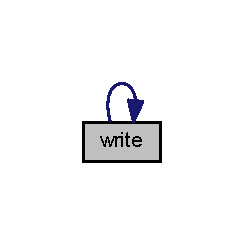
\includegraphics[width=117pt]{class_hardware_serial_a0ba52a995edf9b6c2cdf3d396be84ff1_cgraph}
\end{center}
\end{figure}




Here is the caller graph for this function\+:\nopagebreak
\begin{figure}[H]
\begin{center}
\leavevmode
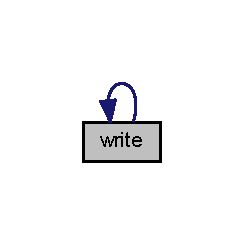
\includegraphics[width=117pt]{class_hardware_serial_a0ba52a995edf9b6c2cdf3d396be84ff1_icgraph}
\end{center}
\end{figure}


\hypertarget{class_hardware_serial_a3cfec102ee6f58a2f7e617999ce9f5bb}{}\index{Hardware\+Serial@{Hardware\+Serial}!write@{write}}
\index{write@{write}!Hardware\+Serial@{Hardware\+Serial}}
\subsubsection[{write(long n)}]{\setlength{\rightskip}{0pt plus 5cm}size\+\_\+t write (
\begin{DoxyParamCaption}
\item[{long}]{n}
\end{DoxyParamCaption}
)\hspace{0.3cm}{\ttfamily [inline]}}\label{class_hardware_serial_a3cfec102ee6f58a2f7e617999ce9f5bb}


Definition at line 121 of file Hardware\+Serial.\+h.



Here is the call graph for this function\+:\nopagebreak
\begin{figure}[H]
\begin{center}
\leavevmode
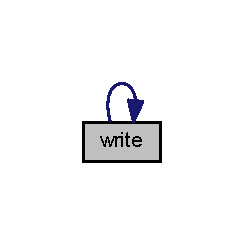
\includegraphics[width=117pt]{class_hardware_serial_a3cfec102ee6f58a2f7e617999ce9f5bb_cgraph}
\end{center}
\end{figure}




Here is the caller graph for this function\+:\nopagebreak
\begin{figure}[H]
\begin{center}
\leavevmode
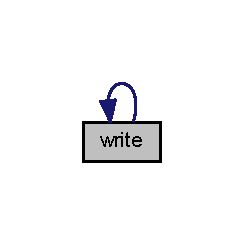
\includegraphics[width=117pt]{class_hardware_serial_a3cfec102ee6f58a2f7e617999ce9f5bb_icgraph}
\end{center}
\end{figure}


\hypertarget{class_hardware_serial_a2d9bc6ac05e45a7023be3cd1ca224407}{}\index{Hardware\+Serial@{Hardware\+Serial}!write@{write}}
\index{write@{write}!Hardware\+Serial@{Hardware\+Serial}}
\subsubsection[{write(unsigned int n)}]{\setlength{\rightskip}{0pt plus 5cm}size\+\_\+t write (
\begin{DoxyParamCaption}
\item[{unsigned int}]{n}
\end{DoxyParamCaption}
)\hspace{0.3cm}{\ttfamily [inline]}}\label{class_hardware_serial_a2d9bc6ac05e45a7023be3cd1ca224407}


Definition at line 122 of file Hardware\+Serial.\+h.



Here is the call graph for this function\+:\nopagebreak
\begin{figure}[H]
\begin{center}
\leavevmode
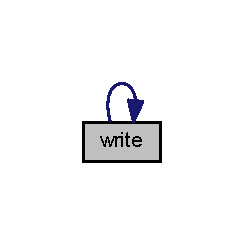
\includegraphics[width=117pt]{class_hardware_serial_a2d9bc6ac05e45a7023be3cd1ca224407_cgraph}
\end{center}
\end{figure}




Here is the caller graph for this function\+:\nopagebreak
\begin{figure}[H]
\begin{center}
\leavevmode
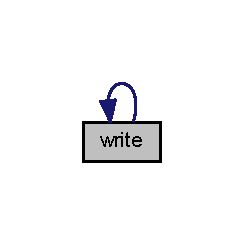
\includegraphics[width=117pt]{class_hardware_serial_a2d9bc6ac05e45a7023be3cd1ca224407_icgraph}
\end{center}
\end{figure}


\hypertarget{class_hardware_serial_a22e7ab55e0aa268cff5b48e763429ec3}{}\index{Hardware\+Serial@{Hardware\+Serial}!write@{write}}
\index{write@{write}!Hardware\+Serial@{Hardware\+Serial}}
\subsubsection[{write(int n)}]{\setlength{\rightskip}{0pt plus 5cm}size\+\_\+t write (
\begin{DoxyParamCaption}
\item[{int}]{n}
\end{DoxyParamCaption}
)\hspace{0.3cm}{\ttfamily [inline]}}\label{class_hardware_serial_a22e7ab55e0aa268cff5b48e763429ec3}


Definition at line 123 of file Hardware\+Serial.\+h.



Here is the call graph for this function\+:\nopagebreak
\begin{figure}[H]
\begin{center}
\leavevmode
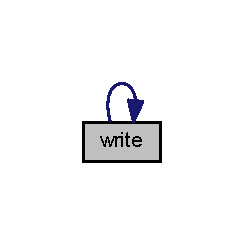
\includegraphics[width=117pt]{class_hardware_serial_a22e7ab55e0aa268cff5b48e763429ec3_cgraph}
\end{center}
\end{figure}




Here is the caller graph for this function\+:\nopagebreak
\begin{figure}[H]
\begin{center}
\leavevmode
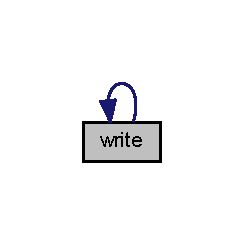
\includegraphics[width=117pt]{class_hardware_serial_a22e7ab55e0aa268cff5b48e763429ec3_icgraph}
\end{center}
\end{figure}




\subsection{Field Documentation}
\hypertarget{class_hardware_serial_ae33d584001d6c3fbbc6a8097b0ab19c7}{}\index{Hardware\+Serial@{Hardware\+Serial}!\+\_\+rx\+\_\+buffer@{\+\_\+rx\+\_\+buffer}}
\index{\+\_\+rx\+\_\+buffer@{\+\_\+rx\+\_\+buffer}!Hardware\+Serial@{Hardware\+Serial}}
\subsubsection[{\+\_\+rx\+\_\+buffer}]{\setlength{\rightskip}{0pt plus 5cm}unsigned char \+\_\+rx\+\_\+buffer\mbox{[}{\bf S\+E\+R\+I\+A\+L\+\_\+\+R\+X\+\_\+\+B\+U\+F\+F\+E\+R\+\_\+\+S\+I\+Z\+E}\mbox{]}\hspace{0.3cm}{\ttfamily [protected]}}\label{class_hardware_serial_ae33d584001d6c3fbbc6a8097b0ab19c7}


Definition at line 103 of file Hardware\+Serial.\+h.

\hypertarget{class_hardware_serial_a797ebcc80bc2806b3ebbfc509e7aeabe}{}\index{Hardware\+Serial@{Hardware\+Serial}!\+\_\+rx\+\_\+buffer\+\_\+head@{\+\_\+rx\+\_\+buffer\+\_\+head}}
\index{\+\_\+rx\+\_\+buffer\+\_\+head@{\+\_\+rx\+\_\+buffer\+\_\+head}!Hardware\+Serial@{Hardware\+Serial}}
\subsubsection[{\+\_\+rx\+\_\+buffer\+\_\+head}]{\setlength{\rightskip}{0pt plus 5cm}volatile {\bf rx\+\_\+buffer\+\_\+index\+\_\+t} \+\_\+rx\+\_\+buffer\+\_\+head\hspace{0.3cm}{\ttfamily [protected]}}\label{class_hardware_serial_a797ebcc80bc2806b3ebbfc509e7aeabe}


Definition at line 95 of file Hardware\+Serial.\+h.

\hypertarget{class_hardware_serial_a0343d5d99eb23a56dd3ad5b48928a94a}{}\index{Hardware\+Serial@{Hardware\+Serial}!\+\_\+rx\+\_\+buffer\+\_\+tail@{\+\_\+rx\+\_\+buffer\+\_\+tail}}
\index{\+\_\+rx\+\_\+buffer\+\_\+tail@{\+\_\+rx\+\_\+buffer\+\_\+tail}!Hardware\+Serial@{Hardware\+Serial}}
\subsubsection[{\+\_\+rx\+\_\+buffer\+\_\+tail}]{\setlength{\rightskip}{0pt plus 5cm}volatile {\bf rx\+\_\+buffer\+\_\+index\+\_\+t} \+\_\+rx\+\_\+buffer\+\_\+tail\hspace{0.3cm}{\ttfamily [protected]}}\label{class_hardware_serial_a0343d5d99eb23a56dd3ad5b48928a94a}


Definition at line 96 of file Hardware\+Serial.\+h.

\hypertarget{class_hardware_serial_ae29711a762cbc9a7f622b4f4ff64d374}{}\index{Hardware\+Serial@{Hardware\+Serial}!\+\_\+tx\+\_\+buffer@{\+\_\+tx\+\_\+buffer}}
\index{\+\_\+tx\+\_\+buffer@{\+\_\+tx\+\_\+buffer}!Hardware\+Serial@{Hardware\+Serial}}
\subsubsection[{\+\_\+tx\+\_\+buffer}]{\setlength{\rightskip}{0pt plus 5cm}unsigned char \+\_\+tx\+\_\+buffer\mbox{[}{\bf S\+E\+R\+I\+A\+L\+\_\+\+T\+X\+\_\+\+B\+U\+F\+F\+E\+R\+\_\+\+S\+I\+Z\+E}\mbox{]}\hspace{0.3cm}{\ttfamily [protected]}}\label{class_hardware_serial_ae29711a762cbc9a7f622b4f4ff64d374}


Definition at line 104 of file Hardware\+Serial.\+h.

\hypertarget{class_hardware_serial_abc7b62797e816bc704bfe3ec80f68607}{}\index{Hardware\+Serial@{Hardware\+Serial}!\+\_\+tx\+\_\+buffer\+\_\+head@{\+\_\+tx\+\_\+buffer\+\_\+head}}
\index{\+\_\+tx\+\_\+buffer\+\_\+head@{\+\_\+tx\+\_\+buffer\+\_\+head}!Hardware\+Serial@{Hardware\+Serial}}
\subsubsection[{\+\_\+tx\+\_\+buffer\+\_\+head}]{\setlength{\rightskip}{0pt plus 5cm}volatile {\bf tx\+\_\+buffer\+\_\+index\+\_\+t} \+\_\+tx\+\_\+buffer\+\_\+head\hspace{0.3cm}{\ttfamily [protected]}}\label{class_hardware_serial_abc7b62797e816bc704bfe3ec80f68607}


Definition at line 97 of file Hardware\+Serial.\+h.

\hypertarget{class_hardware_serial_a3aad9ccd1bebab9d9226e0c38ee54465}{}\index{Hardware\+Serial@{Hardware\+Serial}!\+\_\+tx\+\_\+buffer\+\_\+tail@{\+\_\+tx\+\_\+buffer\+\_\+tail}}
\index{\+\_\+tx\+\_\+buffer\+\_\+tail@{\+\_\+tx\+\_\+buffer\+\_\+tail}!Hardware\+Serial@{Hardware\+Serial}}
\subsubsection[{\+\_\+tx\+\_\+buffer\+\_\+tail}]{\setlength{\rightskip}{0pt plus 5cm}volatile {\bf tx\+\_\+buffer\+\_\+index\+\_\+t} \+\_\+tx\+\_\+buffer\+\_\+tail\hspace{0.3cm}{\ttfamily [protected]}}\label{class_hardware_serial_a3aad9ccd1bebab9d9226e0c38ee54465}


Definition at line 98 of file Hardware\+Serial.\+h.

\hypertarget{class_hardware_serial_ac2dd0caa2b74a2992e1b9b0d63dec696}{}\index{Hardware\+Serial@{Hardware\+Serial}!\+\_\+ubrrh@{\+\_\+ubrrh}}
\index{\+\_\+ubrrh@{\+\_\+ubrrh}!Hardware\+Serial@{Hardware\+Serial}}
\subsubsection[{\+\_\+ubrrh}]{\setlength{\rightskip}{0pt plus 5cm}volatile uint8\+\_\+t$\ast$ const \+\_\+ubrrh\hspace{0.3cm}{\ttfamily [protected]}}\label{class_hardware_serial_ac2dd0caa2b74a2992e1b9b0d63dec696}


Definition at line 86 of file Hardware\+Serial.\+h.

\hypertarget{class_hardware_serial_ad61fd40f665d597de97ec3995e251e93}{}\index{Hardware\+Serial@{Hardware\+Serial}!\+\_\+ubrrl@{\+\_\+ubrrl}}
\index{\+\_\+ubrrl@{\+\_\+ubrrl}!Hardware\+Serial@{Hardware\+Serial}}
\subsubsection[{\+\_\+ubrrl}]{\setlength{\rightskip}{0pt plus 5cm}volatile uint8\+\_\+t$\ast$ const \+\_\+ubrrl\hspace{0.3cm}{\ttfamily [protected]}}\label{class_hardware_serial_ad61fd40f665d597de97ec3995e251e93}


Definition at line 87 of file Hardware\+Serial.\+h.

\hypertarget{class_hardware_serial_a691bd409418c1acc6fc583692b54764f}{}\index{Hardware\+Serial@{Hardware\+Serial}!\+\_\+ucsra@{\+\_\+ucsra}}
\index{\+\_\+ucsra@{\+\_\+ucsra}!Hardware\+Serial@{Hardware\+Serial}}
\subsubsection[{\+\_\+ucsra}]{\setlength{\rightskip}{0pt plus 5cm}volatile uint8\+\_\+t$\ast$ const \+\_\+ucsra\hspace{0.3cm}{\ttfamily [protected]}}\label{class_hardware_serial_a691bd409418c1acc6fc583692b54764f}


Definition at line 88 of file Hardware\+Serial.\+h.

\hypertarget{class_hardware_serial_a06c3d929aa3eb0e48227139d1750a3a7}{}\index{Hardware\+Serial@{Hardware\+Serial}!\+\_\+ucsrb@{\+\_\+ucsrb}}
\index{\+\_\+ucsrb@{\+\_\+ucsrb}!Hardware\+Serial@{Hardware\+Serial}}
\subsubsection[{\+\_\+ucsrb}]{\setlength{\rightskip}{0pt plus 5cm}volatile uint8\+\_\+t$\ast$ const \+\_\+ucsrb\hspace{0.3cm}{\ttfamily [protected]}}\label{class_hardware_serial_a06c3d929aa3eb0e48227139d1750a3a7}


Definition at line 89 of file Hardware\+Serial.\+h.

\hypertarget{class_hardware_serial_a3599c284453c515776147539d753d1bf}{}\index{Hardware\+Serial@{Hardware\+Serial}!\+\_\+ucsrc@{\+\_\+ucsrc}}
\index{\+\_\+ucsrc@{\+\_\+ucsrc}!Hardware\+Serial@{Hardware\+Serial}}
\subsubsection[{\+\_\+ucsrc}]{\setlength{\rightskip}{0pt plus 5cm}volatile uint8\+\_\+t$\ast$ const \+\_\+ucsrc\hspace{0.3cm}{\ttfamily [protected]}}\label{class_hardware_serial_a3599c284453c515776147539d753d1bf}


Definition at line 90 of file Hardware\+Serial.\+h.

\hypertarget{class_hardware_serial_a9123daf6c7d2bc8c3997d73f7b30bece}{}\index{Hardware\+Serial@{Hardware\+Serial}!\+\_\+udr@{\+\_\+udr}}
\index{\+\_\+udr@{\+\_\+udr}!Hardware\+Serial@{Hardware\+Serial}}
\subsubsection[{\+\_\+udr}]{\setlength{\rightskip}{0pt plus 5cm}volatile uint8\+\_\+t$\ast$ const \+\_\+udr\hspace{0.3cm}{\ttfamily [protected]}}\label{class_hardware_serial_a9123daf6c7d2bc8c3997d73f7b30bece}


Definition at line 91 of file Hardware\+Serial.\+h.

\hypertarget{class_hardware_serial_a491255f295202ef6556a978224fdc71e}{}\index{Hardware\+Serial@{Hardware\+Serial}!\+\_\+written@{\+\_\+written}}
\index{\+\_\+written@{\+\_\+written}!Hardware\+Serial@{Hardware\+Serial}}
\subsubsection[{\+\_\+written}]{\setlength{\rightskip}{0pt plus 5cm}bool \+\_\+written\hspace{0.3cm}{\ttfamily [protected]}}\label{class_hardware_serial_a491255f295202ef6556a978224fdc71e}


Definition at line 93 of file Hardware\+Serial.\+h.



The documentation for this class was generated from the following file\+:\begin{DoxyCompactItemize}
\item 
Arduino\+U\+N\+O/src/arduino/cores/arduino/\hyperlink{_hardware_serial_8h}{Hardware\+Serial.\+h}\end{DoxyCompactItemize}

\hypertarget{struct_h_i_d_desc_descriptor}{}\section{H\+I\+D\+Desc\+Descriptor Struct Reference}
\label{struct_h_i_d_desc_descriptor}\index{H\+I\+D\+Desc\+Descriptor@{H\+I\+D\+Desc\+Descriptor}}


{\ttfamily \#include $<$U\+S\+B\+Core.\+h$>$}

\subsection*{Data Fields}
\begin{DoxyCompactItemize}
\item 
\hyperlink{_u_s_b_a_p_i_8h_aed742c436da53c1080638ce6ef7d13de}{u8} \hyperlink{struct_h_i_d_desc_descriptor_afbf3f3230446569534d5f466aaf4c23b}{len}
\item 
\hyperlink{_u_s_b_a_p_i_8h_aed742c436da53c1080638ce6ef7d13de}{u8} \hyperlink{struct_h_i_d_desc_descriptor_a0bb419531ec75697e63e9109fecf81b0}{dtype}
\item 
\hyperlink{_u_s_b_a_p_i_8h_aed742c436da53c1080638ce6ef7d13de}{u8} \hyperlink{struct_h_i_d_desc_descriptor_a7394c0f7cac587defeae4e84d34fb535}{addr}
\item 
\hyperlink{_u_s_b_a_p_i_8h_aed742c436da53c1080638ce6ef7d13de}{u8} \hyperlink{struct_h_i_d_desc_descriptor_abbe47c1ab026892a2d5ed0c8690f63c4}{version\+L}
\item 
\hyperlink{_u_s_b_a_p_i_8h_aed742c436da53c1080638ce6ef7d13de}{u8} \hyperlink{struct_h_i_d_desc_descriptor_a25c3b37fcec9c0b6cd0b3aaa62c904f0}{version\+H}
\item 
\hyperlink{_u_s_b_a_p_i_8h_aed742c436da53c1080638ce6ef7d13de}{u8} \hyperlink{struct_h_i_d_desc_descriptor_adf7dd313d5179831aef0bd2c06e7fb37}{country}
\item 
\hyperlink{_u_s_b_a_p_i_8h_aed742c436da53c1080638ce6ef7d13de}{u8} \hyperlink{struct_h_i_d_desc_descriptor_ab7b17f5a1f2d18b4fb7f406b6b80d8be}{desctype}
\item 
\hyperlink{_u_s_b_a_p_i_8h_aed742c436da53c1080638ce6ef7d13de}{u8} \hyperlink{struct_h_i_d_desc_descriptor_ab79e949a76fd9f11acbeda14f76b41d6}{desc\+Len\+L}
\item 
\hyperlink{_u_s_b_a_p_i_8h_aed742c436da53c1080638ce6ef7d13de}{u8} \hyperlink{struct_h_i_d_desc_descriptor_acb9cb52171317c0ea8140dd491c0d00e}{desc\+Len\+H}
\end{DoxyCompactItemize}


\subsection{Detailed Description}


Definition at line 260 of file U\+S\+B\+Core.\+h.



\subsection{Field Documentation}
\hypertarget{struct_h_i_d_desc_descriptor_a7394c0f7cac587defeae4e84d34fb535}{}\index{H\+I\+D\+Desc\+Descriptor@{H\+I\+D\+Desc\+Descriptor}!addr@{addr}}
\index{addr@{addr}!H\+I\+D\+Desc\+Descriptor@{H\+I\+D\+Desc\+Descriptor}}
\subsubsection[{addr}]{\setlength{\rightskip}{0pt plus 5cm}{\bf u8} addr}\label{struct_h_i_d_desc_descriptor_a7394c0f7cac587defeae4e84d34fb535}


Definition at line 264 of file U\+S\+B\+Core.\+h.

\hypertarget{struct_h_i_d_desc_descriptor_adf7dd313d5179831aef0bd2c06e7fb37}{}\index{H\+I\+D\+Desc\+Descriptor@{H\+I\+D\+Desc\+Descriptor}!country@{country}}
\index{country@{country}!H\+I\+D\+Desc\+Descriptor@{H\+I\+D\+Desc\+Descriptor}}
\subsubsection[{country}]{\setlength{\rightskip}{0pt plus 5cm}{\bf u8} country}\label{struct_h_i_d_desc_descriptor_adf7dd313d5179831aef0bd2c06e7fb37}


Definition at line 267 of file U\+S\+B\+Core.\+h.

\hypertarget{struct_h_i_d_desc_descriptor_acb9cb52171317c0ea8140dd491c0d00e}{}\index{H\+I\+D\+Desc\+Descriptor@{H\+I\+D\+Desc\+Descriptor}!desc\+Len\+H@{desc\+Len\+H}}
\index{desc\+Len\+H@{desc\+Len\+H}!H\+I\+D\+Desc\+Descriptor@{H\+I\+D\+Desc\+Descriptor}}
\subsubsection[{desc\+Len\+H}]{\setlength{\rightskip}{0pt plus 5cm}{\bf u8} desc\+Len\+H}\label{struct_h_i_d_desc_descriptor_acb9cb52171317c0ea8140dd491c0d00e}


Definition at line 270 of file U\+S\+B\+Core.\+h.

\hypertarget{struct_h_i_d_desc_descriptor_ab79e949a76fd9f11acbeda14f76b41d6}{}\index{H\+I\+D\+Desc\+Descriptor@{H\+I\+D\+Desc\+Descriptor}!desc\+Len\+L@{desc\+Len\+L}}
\index{desc\+Len\+L@{desc\+Len\+L}!H\+I\+D\+Desc\+Descriptor@{H\+I\+D\+Desc\+Descriptor}}
\subsubsection[{desc\+Len\+L}]{\setlength{\rightskip}{0pt plus 5cm}{\bf u8} desc\+Len\+L}\label{struct_h_i_d_desc_descriptor_ab79e949a76fd9f11acbeda14f76b41d6}


Definition at line 269 of file U\+S\+B\+Core.\+h.

\hypertarget{struct_h_i_d_desc_descriptor_ab7b17f5a1f2d18b4fb7f406b6b80d8be}{}\index{H\+I\+D\+Desc\+Descriptor@{H\+I\+D\+Desc\+Descriptor}!desctype@{desctype}}
\index{desctype@{desctype}!H\+I\+D\+Desc\+Descriptor@{H\+I\+D\+Desc\+Descriptor}}
\subsubsection[{desctype}]{\setlength{\rightskip}{0pt plus 5cm}{\bf u8} desctype}\label{struct_h_i_d_desc_descriptor_ab7b17f5a1f2d18b4fb7f406b6b80d8be}


Definition at line 268 of file U\+S\+B\+Core.\+h.

\hypertarget{struct_h_i_d_desc_descriptor_a0bb419531ec75697e63e9109fecf81b0}{}\index{H\+I\+D\+Desc\+Descriptor@{H\+I\+D\+Desc\+Descriptor}!dtype@{dtype}}
\index{dtype@{dtype}!H\+I\+D\+Desc\+Descriptor@{H\+I\+D\+Desc\+Descriptor}}
\subsubsection[{dtype}]{\setlength{\rightskip}{0pt plus 5cm}{\bf u8} dtype}\label{struct_h_i_d_desc_descriptor_a0bb419531ec75697e63e9109fecf81b0}


Definition at line 263 of file U\+S\+B\+Core.\+h.

\hypertarget{struct_h_i_d_desc_descriptor_afbf3f3230446569534d5f466aaf4c23b}{}\index{H\+I\+D\+Desc\+Descriptor@{H\+I\+D\+Desc\+Descriptor}!len@{len}}
\index{len@{len}!H\+I\+D\+Desc\+Descriptor@{H\+I\+D\+Desc\+Descriptor}}
\subsubsection[{len}]{\setlength{\rightskip}{0pt plus 5cm}{\bf u8} len}\label{struct_h_i_d_desc_descriptor_afbf3f3230446569534d5f466aaf4c23b}


Definition at line 262 of file U\+S\+B\+Core.\+h.

\hypertarget{struct_h_i_d_desc_descriptor_a25c3b37fcec9c0b6cd0b3aaa62c904f0}{}\index{H\+I\+D\+Desc\+Descriptor@{H\+I\+D\+Desc\+Descriptor}!version\+H@{version\+H}}
\index{version\+H@{version\+H}!H\+I\+D\+Desc\+Descriptor@{H\+I\+D\+Desc\+Descriptor}}
\subsubsection[{version\+H}]{\setlength{\rightskip}{0pt plus 5cm}{\bf u8} version\+H}\label{struct_h_i_d_desc_descriptor_a25c3b37fcec9c0b6cd0b3aaa62c904f0}


Definition at line 266 of file U\+S\+B\+Core.\+h.

\hypertarget{struct_h_i_d_desc_descriptor_abbe47c1ab026892a2d5ed0c8690f63c4}{}\index{H\+I\+D\+Desc\+Descriptor@{H\+I\+D\+Desc\+Descriptor}!version\+L@{version\+L}}
\index{version\+L@{version\+L}!H\+I\+D\+Desc\+Descriptor@{H\+I\+D\+Desc\+Descriptor}}
\subsubsection[{version\+L}]{\setlength{\rightskip}{0pt plus 5cm}{\bf u8} version\+L}\label{struct_h_i_d_desc_descriptor_abbe47c1ab026892a2d5ed0c8690f63c4}


Definition at line 265 of file U\+S\+B\+Core.\+h.



The documentation for this struct was generated from the following file\+:\begin{DoxyCompactItemize}
\item 
Arduino\+U\+N\+O/src/arduino/cores/arduino/\hyperlink{_u_s_b_core_8h}{U\+S\+B\+Core.\+h}\end{DoxyCompactItemize}

\hypertarget{struct_h_i_d_descriptor}{}\section{H\+I\+D\+Descriptor Struct Reference}
\label{struct_h_i_d_descriptor}\index{H\+I\+D\+Descriptor@{H\+I\+D\+Descriptor}}


{\ttfamily \#include $<$U\+S\+B\+Core.\+h$>$}



Collaboration diagram for H\+I\+D\+Descriptor\+:\nopagebreak
\begin{figure}[H]
\begin{center}
\leavevmode
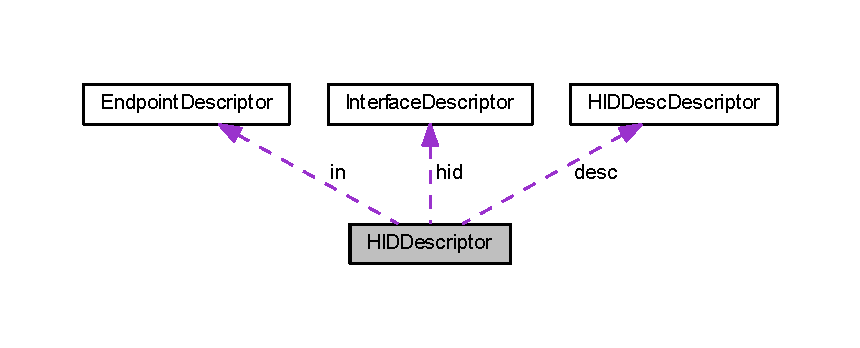
\includegraphics[width=350pt]{struct_h_i_d_descriptor__coll__graph}
\end{center}
\end{figure}
\subsection*{Data Fields}
\begin{DoxyCompactItemize}
\item 
\hyperlink{struct_interface_descriptor}{Interface\+Descriptor} \hyperlink{struct_h_i_d_descriptor_a81907e74fcb6fd20130a4a921e4be5fd}{hid}
\item 
\hyperlink{struct_h_i_d_desc_descriptor}{H\+I\+D\+Desc\+Descriptor} \hyperlink{struct_h_i_d_descriptor_ae46b89dcb6c43addf455fc25ebbf9963}{desc}
\item 
\hyperlink{struct_endpoint_descriptor}{Endpoint\+Descriptor} \hyperlink{struct_h_i_d_descriptor_a93dcef3b3e3062b904269bcad94771b5}{in}
\end{DoxyCompactItemize}


\subsection{Detailed Description}


Definition at line 273 of file U\+S\+B\+Core.\+h.



\subsection{Field Documentation}
\hypertarget{struct_h_i_d_descriptor_ae46b89dcb6c43addf455fc25ebbf9963}{}\index{H\+I\+D\+Descriptor@{H\+I\+D\+Descriptor}!desc@{desc}}
\index{desc@{desc}!H\+I\+D\+Descriptor@{H\+I\+D\+Descriptor}}
\subsubsection[{desc}]{\setlength{\rightskip}{0pt plus 5cm}{\bf H\+I\+D\+Desc\+Descriptor} desc}\label{struct_h_i_d_descriptor_ae46b89dcb6c43addf455fc25ebbf9963}


Definition at line 276 of file U\+S\+B\+Core.\+h.

\hypertarget{struct_h_i_d_descriptor_a81907e74fcb6fd20130a4a921e4be5fd}{}\index{H\+I\+D\+Descriptor@{H\+I\+D\+Descriptor}!hid@{hid}}
\index{hid@{hid}!H\+I\+D\+Descriptor@{H\+I\+D\+Descriptor}}
\subsubsection[{hid}]{\setlength{\rightskip}{0pt plus 5cm}{\bf Interface\+Descriptor} hid}\label{struct_h_i_d_descriptor_a81907e74fcb6fd20130a4a921e4be5fd}


Definition at line 275 of file U\+S\+B\+Core.\+h.

\hypertarget{struct_h_i_d_descriptor_a93dcef3b3e3062b904269bcad94771b5}{}\index{H\+I\+D\+Descriptor@{H\+I\+D\+Descriptor}!in@{in}}
\index{in@{in}!H\+I\+D\+Descriptor@{H\+I\+D\+Descriptor}}
\subsubsection[{in}]{\setlength{\rightskip}{0pt plus 5cm}{\bf Endpoint\+Descriptor} in}\label{struct_h_i_d_descriptor_a93dcef3b3e3062b904269bcad94771b5}


Definition at line 277 of file U\+S\+B\+Core.\+h.



The documentation for this struct was generated from the following file\+:\begin{DoxyCompactItemize}
\item 
Arduino\+U\+N\+O/src/arduino/cores/arduino/\hyperlink{_u_s_b_core_8h}{U\+S\+B\+Core.\+h}\end{DoxyCompactItemize}

\hypertarget{struct_i_a_d_descriptor}{}\section{I\+A\+D\+Descriptor Struct Reference}
\label{struct_i_a_d_descriptor}\index{I\+A\+D\+Descriptor@{I\+A\+D\+Descriptor}}


{\ttfamily \#include $<$U\+S\+B\+Core.\+h$>$}

\subsection*{Data Fields}
\begin{DoxyCompactItemize}
\item 
\hyperlink{_u_s_b_a_p_i_8h_aed742c436da53c1080638ce6ef7d13de}{u8} \hyperlink{struct_i_a_d_descriptor_afbf3f3230446569534d5f466aaf4c23b}{len}
\item 
\hyperlink{_u_s_b_a_p_i_8h_aed742c436da53c1080638ce6ef7d13de}{u8} \hyperlink{struct_i_a_d_descriptor_a0bb419531ec75697e63e9109fecf81b0}{dtype}
\item 
\hyperlink{_u_s_b_a_p_i_8h_aed742c436da53c1080638ce6ef7d13de}{u8} \hyperlink{struct_i_a_d_descriptor_a1f310829bc6b0452ca7a433306711834}{first\+Interface}
\item 
\hyperlink{_u_s_b_a_p_i_8h_aed742c436da53c1080638ce6ef7d13de}{u8} \hyperlink{struct_i_a_d_descriptor_ace4364c3a11490d83a57929409bab191}{interface\+Count}
\item 
\hyperlink{_u_s_b_a_p_i_8h_aed742c436da53c1080638ce6ef7d13de}{u8} \hyperlink{struct_i_a_d_descriptor_acf3f3dd7456fc16e020aff6bbe0f9573}{function\+Class}
\item 
\hyperlink{_u_s_b_a_p_i_8h_aed742c436da53c1080638ce6ef7d13de}{u8} \hyperlink{struct_i_a_d_descriptor_a6e072e7ab27ae52a925d022757a6abd1}{funtion\+Sub\+Class}
\item 
\hyperlink{_u_s_b_a_p_i_8h_aed742c436da53c1080638ce6ef7d13de}{u8} \hyperlink{struct_i_a_d_descriptor_a451c6c7831d9e3e3898951c5d036081f}{function\+Protocol}
\item 
\hyperlink{_u_s_b_a_p_i_8h_aed742c436da53c1080638ce6ef7d13de}{u8} \hyperlink{struct_i_a_d_descriptor_a08ba0e1160648c2e45d24d1f00484466}{i\+Interface}
\end{DoxyCompactItemize}


\subsection{Detailed Description}


Definition at line 187 of file U\+S\+B\+Core.\+h.



\subsection{Field Documentation}
\hypertarget{struct_i_a_d_descriptor_a0bb419531ec75697e63e9109fecf81b0}{}\index{I\+A\+D\+Descriptor@{I\+A\+D\+Descriptor}!dtype@{dtype}}
\index{dtype@{dtype}!I\+A\+D\+Descriptor@{I\+A\+D\+Descriptor}}
\subsubsection[{dtype}]{\setlength{\rightskip}{0pt plus 5cm}{\bf u8} dtype}\label{struct_i_a_d_descriptor_a0bb419531ec75697e63e9109fecf81b0}


Definition at line 190 of file U\+S\+B\+Core.\+h.

\hypertarget{struct_i_a_d_descriptor_a1f310829bc6b0452ca7a433306711834}{}\index{I\+A\+D\+Descriptor@{I\+A\+D\+Descriptor}!first\+Interface@{first\+Interface}}
\index{first\+Interface@{first\+Interface}!I\+A\+D\+Descriptor@{I\+A\+D\+Descriptor}}
\subsubsection[{first\+Interface}]{\setlength{\rightskip}{0pt plus 5cm}{\bf u8} first\+Interface}\label{struct_i_a_d_descriptor_a1f310829bc6b0452ca7a433306711834}


Definition at line 191 of file U\+S\+B\+Core.\+h.

\hypertarget{struct_i_a_d_descriptor_acf3f3dd7456fc16e020aff6bbe0f9573}{}\index{I\+A\+D\+Descriptor@{I\+A\+D\+Descriptor}!function\+Class@{function\+Class}}
\index{function\+Class@{function\+Class}!I\+A\+D\+Descriptor@{I\+A\+D\+Descriptor}}
\subsubsection[{function\+Class}]{\setlength{\rightskip}{0pt plus 5cm}{\bf u8} function\+Class}\label{struct_i_a_d_descriptor_acf3f3dd7456fc16e020aff6bbe0f9573}


Definition at line 193 of file U\+S\+B\+Core.\+h.

\hypertarget{struct_i_a_d_descriptor_a451c6c7831d9e3e3898951c5d036081f}{}\index{I\+A\+D\+Descriptor@{I\+A\+D\+Descriptor}!function\+Protocol@{function\+Protocol}}
\index{function\+Protocol@{function\+Protocol}!I\+A\+D\+Descriptor@{I\+A\+D\+Descriptor}}
\subsubsection[{function\+Protocol}]{\setlength{\rightskip}{0pt plus 5cm}{\bf u8} function\+Protocol}\label{struct_i_a_d_descriptor_a451c6c7831d9e3e3898951c5d036081f}


Definition at line 195 of file U\+S\+B\+Core.\+h.

\hypertarget{struct_i_a_d_descriptor_a6e072e7ab27ae52a925d022757a6abd1}{}\index{I\+A\+D\+Descriptor@{I\+A\+D\+Descriptor}!funtion\+Sub\+Class@{funtion\+Sub\+Class}}
\index{funtion\+Sub\+Class@{funtion\+Sub\+Class}!I\+A\+D\+Descriptor@{I\+A\+D\+Descriptor}}
\subsubsection[{funtion\+Sub\+Class}]{\setlength{\rightskip}{0pt plus 5cm}{\bf u8} funtion\+Sub\+Class}\label{struct_i_a_d_descriptor_a6e072e7ab27ae52a925d022757a6abd1}


Definition at line 194 of file U\+S\+B\+Core.\+h.

\hypertarget{struct_i_a_d_descriptor_a08ba0e1160648c2e45d24d1f00484466}{}\index{I\+A\+D\+Descriptor@{I\+A\+D\+Descriptor}!i\+Interface@{i\+Interface}}
\index{i\+Interface@{i\+Interface}!I\+A\+D\+Descriptor@{I\+A\+D\+Descriptor}}
\subsubsection[{i\+Interface}]{\setlength{\rightskip}{0pt plus 5cm}{\bf u8} i\+Interface}\label{struct_i_a_d_descriptor_a08ba0e1160648c2e45d24d1f00484466}


Definition at line 196 of file U\+S\+B\+Core.\+h.

\hypertarget{struct_i_a_d_descriptor_ace4364c3a11490d83a57929409bab191}{}\index{I\+A\+D\+Descriptor@{I\+A\+D\+Descriptor}!interface\+Count@{interface\+Count}}
\index{interface\+Count@{interface\+Count}!I\+A\+D\+Descriptor@{I\+A\+D\+Descriptor}}
\subsubsection[{interface\+Count}]{\setlength{\rightskip}{0pt plus 5cm}{\bf u8} interface\+Count}\label{struct_i_a_d_descriptor_ace4364c3a11490d83a57929409bab191}


Definition at line 192 of file U\+S\+B\+Core.\+h.

\hypertarget{struct_i_a_d_descriptor_afbf3f3230446569534d5f466aaf4c23b}{}\index{I\+A\+D\+Descriptor@{I\+A\+D\+Descriptor}!len@{len}}
\index{len@{len}!I\+A\+D\+Descriptor@{I\+A\+D\+Descriptor}}
\subsubsection[{len}]{\setlength{\rightskip}{0pt plus 5cm}{\bf u8} len}\label{struct_i_a_d_descriptor_afbf3f3230446569534d5f466aaf4c23b}


Definition at line 189 of file U\+S\+B\+Core.\+h.



The documentation for this struct was generated from the following file\+:\begin{DoxyCompactItemize}
\item 
Arduino\+U\+N\+O/src/arduino/cores/arduino/\hyperlink{_u_s_b_core_8h}{U\+S\+B\+Core.\+h}\end{DoxyCompactItemize}

\hypertarget{struct_interface_descriptor}{}\section{Interface\+Descriptor Struct Reference}
\label{struct_interface_descriptor}\index{Interface\+Descriptor@{Interface\+Descriptor}}


{\ttfamily \#include $<$U\+S\+B\+Core.\+h$>$}

\subsection*{Data Fields}
\begin{DoxyCompactItemize}
\item 
\hyperlink{_u_s_b_a_p_i_8h_aed742c436da53c1080638ce6ef7d13de}{u8} \hyperlink{struct_interface_descriptor_afbf3f3230446569534d5f466aaf4c23b}{len}
\item 
\hyperlink{_u_s_b_a_p_i_8h_aed742c436da53c1080638ce6ef7d13de}{u8} \hyperlink{struct_interface_descriptor_a0bb419531ec75697e63e9109fecf81b0}{dtype}
\item 
\hyperlink{_u_s_b_a_p_i_8h_aed742c436da53c1080638ce6ef7d13de}{u8} \hyperlink{struct_interface_descriptor_a19a3a72d0e5c2ae75bee1ef63637c9e6}{number}
\item 
\hyperlink{_u_s_b_a_p_i_8h_aed742c436da53c1080638ce6ef7d13de}{u8} \hyperlink{struct_interface_descriptor_a8b2cf5542b22d4c9ae79dfe6f7cd6d11}{alternate}
\item 
\hyperlink{_u_s_b_a_p_i_8h_aed742c436da53c1080638ce6ef7d13de}{u8} \hyperlink{struct_interface_descriptor_afe8ecc909a70e40b9aaf4423fb495678}{num\+Endpoints}
\item 
\hyperlink{_u_s_b_a_p_i_8h_aed742c436da53c1080638ce6ef7d13de}{u8} \hyperlink{struct_interface_descriptor_ac54ccb285d7fbe7c6516d4ca1a46d51c}{interface\+Class}
\item 
\hyperlink{_u_s_b_a_p_i_8h_aed742c436da53c1080638ce6ef7d13de}{u8} \hyperlink{struct_interface_descriptor_a9f321d6e124ddf0beadced607fb9208a}{interface\+Sub\+Class}
\item 
\hyperlink{_u_s_b_a_p_i_8h_aed742c436da53c1080638ce6ef7d13de}{u8} \hyperlink{struct_interface_descriptor_a7354e97cb32f39427d6195c914ee2abd}{protocol}
\item 
\hyperlink{_u_s_b_a_p_i_8h_aed742c436da53c1080638ce6ef7d13de}{u8} \hyperlink{struct_interface_descriptor_a08ba0e1160648c2e45d24d1f00484466}{i\+Interface}
\end{DoxyCompactItemize}


\subsection{Detailed Description}


Definition at line 161 of file U\+S\+B\+Core.\+h.



\subsection{Field Documentation}
\hypertarget{struct_interface_descriptor_a8b2cf5542b22d4c9ae79dfe6f7cd6d11}{}\index{Interface\+Descriptor@{Interface\+Descriptor}!alternate@{alternate}}
\index{alternate@{alternate}!Interface\+Descriptor@{Interface\+Descriptor}}
\subsubsection[{alternate}]{\setlength{\rightskip}{0pt plus 5cm}{\bf u8} alternate}\label{struct_interface_descriptor_a8b2cf5542b22d4c9ae79dfe6f7cd6d11}


Definition at line 166 of file U\+S\+B\+Core.\+h.

\hypertarget{struct_interface_descriptor_a0bb419531ec75697e63e9109fecf81b0}{}\index{Interface\+Descriptor@{Interface\+Descriptor}!dtype@{dtype}}
\index{dtype@{dtype}!Interface\+Descriptor@{Interface\+Descriptor}}
\subsubsection[{dtype}]{\setlength{\rightskip}{0pt plus 5cm}{\bf u8} dtype}\label{struct_interface_descriptor_a0bb419531ec75697e63e9109fecf81b0}


Definition at line 164 of file U\+S\+B\+Core.\+h.

\hypertarget{struct_interface_descriptor_a08ba0e1160648c2e45d24d1f00484466}{}\index{Interface\+Descriptor@{Interface\+Descriptor}!i\+Interface@{i\+Interface}}
\index{i\+Interface@{i\+Interface}!Interface\+Descriptor@{Interface\+Descriptor}}
\subsubsection[{i\+Interface}]{\setlength{\rightskip}{0pt plus 5cm}{\bf u8} i\+Interface}\label{struct_interface_descriptor_a08ba0e1160648c2e45d24d1f00484466}


Definition at line 171 of file U\+S\+B\+Core.\+h.

\hypertarget{struct_interface_descriptor_ac54ccb285d7fbe7c6516d4ca1a46d51c}{}\index{Interface\+Descriptor@{Interface\+Descriptor}!interface\+Class@{interface\+Class}}
\index{interface\+Class@{interface\+Class}!Interface\+Descriptor@{Interface\+Descriptor}}
\subsubsection[{interface\+Class}]{\setlength{\rightskip}{0pt plus 5cm}{\bf u8} interface\+Class}\label{struct_interface_descriptor_ac54ccb285d7fbe7c6516d4ca1a46d51c}


Definition at line 168 of file U\+S\+B\+Core.\+h.

\hypertarget{struct_interface_descriptor_a9f321d6e124ddf0beadced607fb9208a}{}\index{Interface\+Descriptor@{Interface\+Descriptor}!interface\+Sub\+Class@{interface\+Sub\+Class}}
\index{interface\+Sub\+Class@{interface\+Sub\+Class}!Interface\+Descriptor@{Interface\+Descriptor}}
\subsubsection[{interface\+Sub\+Class}]{\setlength{\rightskip}{0pt plus 5cm}{\bf u8} interface\+Sub\+Class}\label{struct_interface_descriptor_a9f321d6e124ddf0beadced607fb9208a}


Definition at line 169 of file U\+S\+B\+Core.\+h.

\hypertarget{struct_interface_descriptor_afbf3f3230446569534d5f466aaf4c23b}{}\index{Interface\+Descriptor@{Interface\+Descriptor}!len@{len}}
\index{len@{len}!Interface\+Descriptor@{Interface\+Descriptor}}
\subsubsection[{len}]{\setlength{\rightskip}{0pt plus 5cm}{\bf u8} len}\label{struct_interface_descriptor_afbf3f3230446569534d5f466aaf4c23b}


Definition at line 163 of file U\+S\+B\+Core.\+h.

\hypertarget{struct_interface_descriptor_a19a3a72d0e5c2ae75bee1ef63637c9e6}{}\index{Interface\+Descriptor@{Interface\+Descriptor}!number@{number}}
\index{number@{number}!Interface\+Descriptor@{Interface\+Descriptor}}
\subsubsection[{number}]{\setlength{\rightskip}{0pt plus 5cm}{\bf u8} number}\label{struct_interface_descriptor_a19a3a72d0e5c2ae75bee1ef63637c9e6}


Definition at line 165 of file U\+S\+B\+Core.\+h.

\hypertarget{struct_interface_descriptor_afe8ecc909a70e40b9aaf4423fb495678}{}\index{Interface\+Descriptor@{Interface\+Descriptor}!num\+Endpoints@{num\+Endpoints}}
\index{num\+Endpoints@{num\+Endpoints}!Interface\+Descriptor@{Interface\+Descriptor}}
\subsubsection[{num\+Endpoints}]{\setlength{\rightskip}{0pt plus 5cm}{\bf u8} num\+Endpoints}\label{struct_interface_descriptor_afe8ecc909a70e40b9aaf4423fb495678}


Definition at line 167 of file U\+S\+B\+Core.\+h.

\hypertarget{struct_interface_descriptor_a7354e97cb32f39427d6195c914ee2abd}{}\index{Interface\+Descriptor@{Interface\+Descriptor}!protocol@{protocol}}
\index{protocol@{protocol}!Interface\+Descriptor@{Interface\+Descriptor}}
\subsubsection[{protocol}]{\setlength{\rightskip}{0pt plus 5cm}{\bf u8} protocol}\label{struct_interface_descriptor_a7354e97cb32f39427d6195c914ee2abd}


Definition at line 170 of file U\+S\+B\+Core.\+h.



The documentation for this struct was generated from the following file\+:\begin{DoxyCompactItemize}
\item 
Arduino\+U\+N\+O/src/arduino/cores/arduino/\hyperlink{_u_s_b_core_8h}{U\+S\+B\+Core.\+h}\end{DoxyCompactItemize}

\hypertarget{class_i_p_address}{}\section{I\+P\+Address Class Reference}
\label{class_i_p_address}\index{I\+P\+Address@{I\+P\+Address}}


{\ttfamily \#include $<$I\+P\+Address.\+h$>$}



Inheritance diagram for I\+P\+Address\+:\nopagebreak
\begin{figure}[H]
\begin{center}
\leavevmode
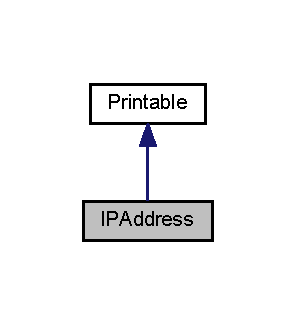
\includegraphics[width=142pt]{class_i_p_address__inherit__graph}
\end{center}
\end{figure}


Collaboration diagram for I\+P\+Address\+:\nopagebreak
\begin{figure}[H]
\begin{center}
\leavevmode
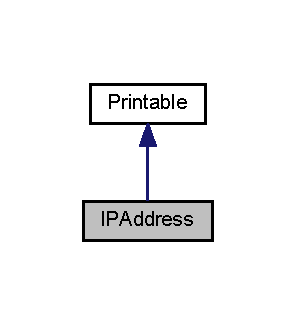
\includegraphics[width=142pt]{class_i_p_address__coll__graph}
\end{center}
\end{figure}
\subsection*{Public Member Functions}
\begin{DoxyCompactItemize}
\item 
\hyperlink{class_i_p_address_a0bfb87befbd8b4cf9ebf348c10a9eaa9}{I\+P\+Address} ()
\item 
\hyperlink{class_i_p_address_a00b68db2117680a85111da0791c0479d}{I\+P\+Address} (uint8\+\_\+t first\+\_\+octet, uint8\+\_\+t second\+\_\+octet, uint8\+\_\+t third\+\_\+octet, uint8\+\_\+t fourth\+\_\+octet)
\item 
\hyperlink{class_i_p_address_a245b8f4f95796da669d51b400ae2b896}{I\+P\+Address} (uint32\+\_\+t address)
\item 
\hyperlink{class_i_p_address_a445de5f4af39b98bf10e8d77832cfe5f}{I\+P\+Address} (const uint8\+\_\+t $\ast$address)
\item 
\hyperlink{class_i_p_address_a07a970954bca44bc378188d2a6332f74}{operator uint32\+\_\+t} () const 
\item 
bool \hyperlink{class_i_p_address_ad0181169c1fa057bf9ef7862ba9f7f84}{operator==} (const \hyperlink{class_i_p_address}{I\+P\+Address} \&addr) const 
\item 
bool \hyperlink{class_i_p_address_a7d473ee4ece3f484491e56ce09096571}{operator==} (const uint8\+\_\+t $\ast$addr) const 
\item 
uint8\+\_\+t \hyperlink{class_i_p_address_a3a30e06242fc12a5aed67bfd77d1b2a5}{operator\mbox{[}$\,$\mbox{]}} (int index) const 
\item 
uint8\+\_\+t \& \hyperlink{class_i_p_address_a362f02e2923dd74e0fc935eab183429d}{operator\mbox{[}$\,$\mbox{]}} (int index)
\item 
\hyperlink{class_i_p_address}{I\+P\+Address} \& \hyperlink{class_i_p_address_ae51d1758e3e7bfdb947bef318c300e7c}{operator=} (const uint8\+\_\+t $\ast$address)
\item 
\hyperlink{class_i_p_address}{I\+P\+Address} \& \hyperlink{class_i_p_address_a1485e06a1694bc174704c61e0d44e52f}{operator=} (uint32\+\_\+t address)
\item 
virtual size\+\_\+t \hyperlink{class_i_p_address_a4de4b3920775530f38f756b2177a9bca}{print\+To} (\hyperlink{class_print}{Print} \&p) const 
\end{DoxyCompactItemize}
\subsection*{Friends}
\begin{DoxyCompactItemize}
\item 
class \hyperlink{class_i_p_address_a9a150ffc237e50529b3d0d50cc83a4d7}{Ethernet\+Class}
\item 
class \hyperlink{class_i_p_address_a480cf93423716d22666c9c3f17177736}{U\+D\+P}
\item 
class \hyperlink{class_i_p_address_a5db1c99e2c94b26278f3838c85cdb618}{Client}
\item 
class \hyperlink{class_i_p_address_ac2055578ac48afabe5af487878450f68}{Server}
\item 
class \hyperlink{class_i_p_address_afef6ad9b691e32ea60d87db719e23e15}{Dhcp\+Class}
\item 
class \hyperlink{class_i_p_address_a14acdf960f52e4a43740d57e81a27c40}{D\+N\+S\+Client}
\end{DoxyCompactItemize}


\subsection{Detailed Description}


Definition at line 28 of file I\+P\+Address.\+h.



\subsection{Constructor \& Destructor Documentation}
\hypertarget{class_i_p_address_a0bfb87befbd8b4cf9ebf348c10a9eaa9}{}\index{I\+P\+Address@{I\+P\+Address}!I\+P\+Address@{I\+P\+Address}}
\index{I\+P\+Address@{I\+P\+Address}!I\+P\+Address@{I\+P\+Address}}
\subsubsection[{I\+P\+Address()}]{\setlength{\rightskip}{0pt plus 5cm}{\bf I\+P\+Address} (
\begin{DoxyParamCaption}
{}
\end{DoxyParamCaption}
)}\label{class_i_p_address_a0bfb87befbd8b4cf9ebf348c10a9eaa9}


Definition at line 23 of file I\+P\+Address.\+cpp.

\hypertarget{class_i_p_address_a00b68db2117680a85111da0791c0479d}{}\index{I\+P\+Address@{I\+P\+Address}!I\+P\+Address@{I\+P\+Address}}
\index{I\+P\+Address@{I\+P\+Address}!I\+P\+Address@{I\+P\+Address}}
\subsubsection[{I\+P\+Address(uint8\+\_\+t first\+\_\+octet, uint8\+\_\+t second\+\_\+octet, uint8\+\_\+t third\+\_\+octet, uint8\+\_\+t fourth\+\_\+octet)}]{\setlength{\rightskip}{0pt plus 5cm}{\bf I\+P\+Address} (
\begin{DoxyParamCaption}
\item[{uint8\+\_\+t}]{first\+\_\+octet, }
\item[{uint8\+\_\+t}]{second\+\_\+octet, }
\item[{uint8\+\_\+t}]{third\+\_\+octet, }
\item[{uint8\+\_\+t}]{fourth\+\_\+octet}
\end{DoxyParamCaption}
)}\label{class_i_p_address_a00b68db2117680a85111da0791c0479d}


Definition at line 28 of file I\+P\+Address.\+cpp.

\hypertarget{class_i_p_address_a245b8f4f95796da669d51b400ae2b896}{}\index{I\+P\+Address@{I\+P\+Address}!I\+P\+Address@{I\+P\+Address}}
\index{I\+P\+Address@{I\+P\+Address}!I\+P\+Address@{I\+P\+Address}}
\subsubsection[{I\+P\+Address(uint32\+\_\+t address)}]{\setlength{\rightskip}{0pt plus 5cm}{\bf I\+P\+Address} (
\begin{DoxyParamCaption}
\item[{uint32\+\_\+t}]{address}
\end{DoxyParamCaption}
)}\label{class_i_p_address_a245b8f4f95796da669d51b400ae2b896}


Definition at line 36 of file I\+P\+Address.\+cpp.

\hypertarget{class_i_p_address_a445de5f4af39b98bf10e8d77832cfe5f}{}\index{I\+P\+Address@{I\+P\+Address}!I\+P\+Address@{I\+P\+Address}}
\index{I\+P\+Address@{I\+P\+Address}!I\+P\+Address@{I\+P\+Address}}
\subsubsection[{I\+P\+Address(const uint8\+\_\+t $\ast$address)}]{\setlength{\rightskip}{0pt plus 5cm}{\bf I\+P\+Address} (
\begin{DoxyParamCaption}
\item[{const uint8\+\_\+t $\ast$}]{address}
\end{DoxyParamCaption}
)}\label{class_i_p_address_a445de5f4af39b98bf10e8d77832cfe5f}


Definition at line 41 of file I\+P\+Address.\+cpp.



\subsection{Member Function Documentation}
\hypertarget{class_i_p_address_a07a970954bca44bc378188d2a6332f74}{}\index{I\+P\+Address@{I\+P\+Address}!operator uint32\+\_\+t@{operator uint32\+\_\+t}}
\index{operator uint32\+\_\+t@{operator uint32\+\_\+t}!I\+P\+Address@{I\+P\+Address}}
\subsubsection[{operator uint32\+\_\+t() const }]{\setlength{\rightskip}{0pt plus 5cm}operator uint32\+\_\+t (
\begin{DoxyParamCaption}
{}
\end{DoxyParamCaption}
) const\hspace{0.3cm}{\ttfamily [inline]}}\label{class_i_p_address_a07a970954bca44bc378188d2a6332f74}


Definition at line 50 of file I\+P\+Address.\+h.

\hypertarget{class_i_p_address_ae51d1758e3e7bfdb947bef318c300e7c}{}\index{I\+P\+Address@{I\+P\+Address}!operator=@{operator=}}
\index{operator=@{operator=}!I\+P\+Address@{I\+P\+Address}}
\subsubsection[{operator=(const uint8\+\_\+t $\ast$address)}]{\setlength{\rightskip}{0pt plus 5cm}{\bf I\+P\+Address} \& operator= (
\begin{DoxyParamCaption}
\item[{const uint8\+\_\+t $\ast$}]{address}
\end{DoxyParamCaption}
)}\label{class_i_p_address_ae51d1758e3e7bfdb947bef318c300e7c}


Definition at line 46 of file I\+P\+Address.\+cpp.

\hypertarget{class_i_p_address_a1485e06a1694bc174704c61e0d44e52f}{}\index{I\+P\+Address@{I\+P\+Address}!operator=@{operator=}}
\index{operator=@{operator=}!I\+P\+Address@{I\+P\+Address}}
\subsubsection[{operator=(uint32\+\_\+t address)}]{\setlength{\rightskip}{0pt plus 5cm}{\bf I\+P\+Address} \& operator= (
\begin{DoxyParamCaption}
\item[{uint32\+\_\+t}]{address}
\end{DoxyParamCaption}
)}\label{class_i_p_address_a1485e06a1694bc174704c61e0d44e52f}


Definition at line 52 of file I\+P\+Address.\+cpp.

\hypertarget{class_i_p_address_ad0181169c1fa057bf9ef7862ba9f7f84}{}\index{I\+P\+Address@{I\+P\+Address}!operator==@{operator==}}
\index{operator==@{operator==}!I\+P\+Address@{I\+P\+Address}}
\subsubsection[{operator==(const I\+P\+Address \&addr) const }]{\setlength{\rightskip}{0pt plus 5cm}bool operator== (
\begin{DoxyParamCaption}
\item[{const {\bf I\+P\+Address} \&}]{addr}
\end{DoxyParamCaption}
) const\hspace{0.3cm}{\ttfamily [inline]}}\label{class_i_p_address_ad0181169c1fa057bf9ef7862ba9f7f84}


Definition at line 51 of file I\+P\+Address.\+h.

\hypertarget{class_i_p_address_a7d473ee4ece3f484491e56ce09096571}{}\index{I\+P\+Address@{I\+P\+Address}!operator==@{operator==}}
\index{operator==@{operator==}!I\+P\+Address@{I\+P\+Address}}
\subsubsection[{operator==(const uint8\+\_\+t $\ast$addr) const }]{\setlength{\rightskip}{0pt plus 5cm}bool operator== (
\begin{DoxyParamCaption}
\item[{const uint8\+\_\+t $\ast$}]{addr}
\end{DoxyParamCaption}
) const}\label{class_i_p_address_a7d473ee4ece3f484491e56ce09096571}


Definition at line 58 of file I\+P\+Address.\+cpp.

\hypertarget{class_i_p_address_a3a30e06242fc12a5aed67bfd77d1b2a5}{}\index{I\+P\+Address@{I\+P\+Address}!operator\mbox{[}$\,$\mbox{]}@{operator[]}}
\index{operator\mbox{[}$\,$\mbox{]}@{operator[]}!I\+P\+Address@{I\+P\+Address}}
\subsubsection[{operator[](int index) const }]{\setlength{\rightskip}{0pt plus 5cm}uint8\+\_\+t operator\mbox{[}$\,$\mbox{]} (
\begin{DoxyParamCaption}
\item[{int}]{index}
\end{DoxyParamCaption}
) const\hspace{0.3cm}{\ttfamily [inline]}}\label{class_i_p_address_a3a30e06242fc12a5aed67bfd77d1b2a5}


Definition at line 55 of file I\+P\+Address.\+h.

\hypertarget{class_i_p_address_a362f02e2923dd74e0fc935eab183429d}{}\index{I\+P\+Address@{I\+P\+Address}!operator\mbox{[}$\,$\mbox{]}@{operator[]}}
\index{operator\mbox{[}$\,$\mbox{]}@{operator[]}!I\+P\+Address@{I\+P\+Address}}
\subsubsection[{operator[](int index)}]{\setlength{\rightskip}{0pt plus 5cm}uint8\+\_\+t\& operator\mbox{[}$\,$\mbox{]} (
\begin{DoxyParamCaption}
\item[{int}]{index}
\end{DoxyParamCaption}
)\hspace{0.3cm}{\ttfamily [inline]}}\label{class_i_p_address_a362f02e2923dd74e0fc935eab183429d}


Definition at line 56 of file I\+P\+Address.\+h.

\hypertarget{class_i_p_address_a4de4b3920775530f38f756b2177a9bca}{}\index{I\+P\+Address@{I\+P\+Address}!print\+To@{print\+To}}
\index{print\+To@{print\+To}!I\+P\+Address@{I\+P\+Address}}
\subsubsection[{print\+To(\+Print \&p) const }]{\setlength{\rightskip}{0pt plus 5cm}size\+\_\+t print\+To (
\begin{DoxyParamCaption}
\item[{{\bf Print} \&}]{p}
\end{DoxyParamCaption}
) const\hspace{0.3cm}{\ttfamily [virtual]}}\label{class_i_p_address_a4de4b3920775530f38f756b2177a9bca}


Implements \hyperlink{class_printable_a95c9f86bb3e38a8743433c80c9250664}{Printable}.



Definition at line 63 of file I\+P\+Address.\+cpp.



Here is the call graph for this function\+:\nopagebreak
\begin{figure}[H]
\begin{center}
\leavevmode
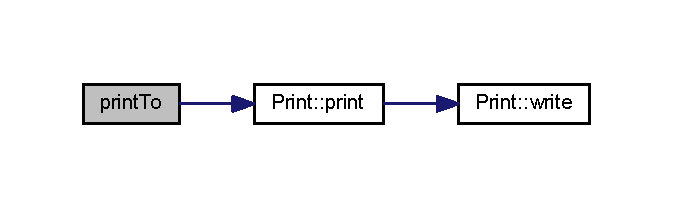
\includegraphics[width=323pt]{class_i_p_address_a4de4b3920775530f38f756b2177a9bca_cgraph}
\end{center}
\end{figure}




\subsection{Friends And Related Function Documentation}
\hypertarget{class_i_p_address_a5db1c99e2c94b26278f3838c85cdb618}{}\index{I\+P\+Address@{I\+P\+Address}!Client@{Client}}
\index{Client@{Client}!I\+P\+Address@{I\+P\+Address}}
\subsubsection[{Client}]{\setlength{\rightskip}{0pt plus 5cm}friend class {\bf Client}\hspace{0.3cm}{\ttfamily [friend]}}\label{class_i_p_address_a5db1c99e2c94b26278f3838c85cdb618}


Definition at line 66 of file I\+P\+Address.\+h.

\hypertarget{class_i_p_address_afef6ad9b691e32ea60d87db719e23e15}{}\index{I\+P\+Address@{I\+P\+Address}!Dhcp\+Class@{Dhcp\+Class}}
\index{Dhcp\+Class@{Dhcp\+Class}!I\+P\+Address@{I\+P\+Address}}
\subsubsection[{Dhcp\+Class}]{\setlength{\rightskip}{0pt plus 5cm}friend class Dhcp\+Class\hspace{0.3cm}{\ttfamily [friend]}}\label{class_i_p_address_afef6ad9b691e32ea60d87db719e23e15}


Definition at line 68 of file I\+P\+Address.\+h.

\hypertarget{class_i_p_address_a14acdf960f52e4a43740d57e81a27c40}{}\index{I\+P\+Address@{I\+P\+Address}!D\+N\+S\+Client@{D\+N\+S\+Client}}
\index{D\+N\+S\+Client@{D\+N\+S\+Client}!I\+P\+Address@{I\+P\+Address}}
\subsubsection[{D\+N\+S\+Client}]{\setlength{\rightskip}{0pt plus 5cm}friend class D\+N\+S\+Client\hspace{0.3cm}{\ttfamily [friend]}}\label{class_i_p_address_a14acdf960f52e4a43740d57e81a27c40}


Definition at line 69 of file I\+P\+Address.\+h.

\hypertarget{class_i_p_address_a9a150ffc237e50529b3d0d50cc83a4d7}{}\index{I\+P\+Address@{I\+P\+Address}!Ethernet\+Class@{Ethernet\+Class}}
\index{Ethernet\+Class@{Ethernet\+Class}!I\+P\+Address@{I\+P\+Address}}
\subsubsection[{Ethernet\+Class}]{\setlength{\rightskip}{0pt plus 5cm}friend class Ethernet\+Class\hspace{0.3cm}{\ttfamily [friend]}}\label{class_i_p_address_a9a150ffc237e50529b3d0d50cc83a4d7}


Definition at line 64 of file I\+P\+Address.\+h.

\hypertarget{class_i_p_address_ac2055578ac48afabe5af487878450f68}{}\index{I\+P\+Address@{I\+P\+Address}!Server@{Server}}
\index{Server@{Server}!I\+P\+Address@{I\+P\+Address}}
\subsubsection[{Server}]{\setlength{\rightskip}{0pt plus 5cm}friend class {\bf Server}\hspace{0.3cm}{\ttfamily [friend]}}\label{class_i_p_address_ac2055578ac48afabe5af487878450f68}


Definition at line 67 of file I\+P\+Address.\+h.

\hypertarget{class_i_p_address_a480cf93423716d22666c9c3f17177736}{}\index{I\+P\+Address@{I\+P\+Address}!U\+D\+P@{U\+D\+P}}
\index{U\+D\+P@{U\+D\+P}!I\+P\+Address@{I\+P\+Address}}
\subsubsection[{U\+D\+P}]{\setlength{\rightskip}{0pt plus 5cm}friend class {\bf U\+D\+P}\hspace{0.3cm}{\ttfamily [friend]}}\label{class_i_p_address_a480cf93423716d22666c9c3f17177736}


Definition at line 65 of file I\+P\+Address.\+h.



\subsection{Field Documentation}
\hypertarget{class_i_p_address_aac9cc4cbc93c66d4b3e0e9e037695d5a}{}\index{I\+P\+Address@{I\+P\+Address}!bytes@{bytes}}
\index{bytes@{bytes}!I\+P\+Address@{I\+P\+Address}}
\subsubsection[{bytes}]{\setlength{\rightskip}{0pt plus 5cm}uint8\+\_\+t bytes\mbox{[}4\mbox{]}}\label{class_i_p_address_aac9cc4cbc93c66d4b3e0e9e037695d5a}


Definition at line 31 of file I\+P\+Address.\+h.

\hypertarget{class_i_p_address_a07145ae3e31b274cc44076fe1681391f}{}\index{I\+P\+Address@{I\+P\+Address}!dword@{dword}}
\index{dword@{dword}!I\+P\+Address@{I\+P\+Address}}
\subsubsection[{dword}]{\setlength{\rightskip}{0pt plus 5cm}uint32\+\_\+t dword}\label{class_i_p_address_a07145ae3e31b274cc44076fe1681391f}


Definition at line 32 of file I\+P\+Address.\+h.



The documentation for this class was generated from the following files\+:\begin{DoxyCompactItemize}
\item 
Arduino\+U\+N\+O/src/arduino/cores/arduino/\hyperlink{_i_p_address_8h}{I\+P\+Address.\+h}\item 
Arduino\+U\+N\+O/src/arduino/cores/arduino/\hyperlink{_i_p_address_8cpp}{I\+P\+Address.\+cpp}\end{DoxyCompactItemize}

\hypertarget{struct_m_s_c_descriptor}{}\section{M\+S\+C\+Descriptor Struct Reference}
\label{struct_m_s_c_descriptor}\index{M\+S\+C\+Descriptor@{M\+S\+C\+Descriptor}}


{\ttfamily \#include $<$U\+S\+B\+Core.\+h$>$}



Collaboration diagram for M\+S\+C\+Descriptor\+:
\nopagebreak
\begin{figure}[H]
\begin{center}
\leavevmode
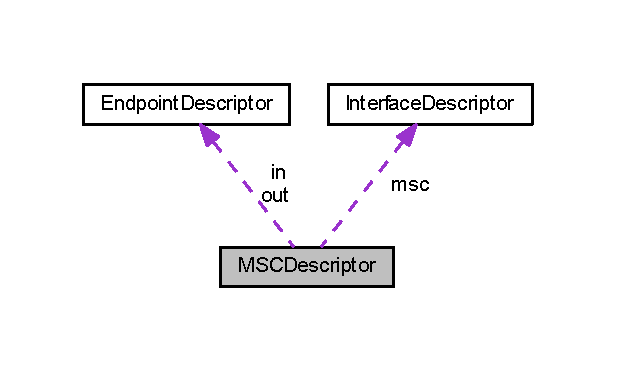
\includegraphics[width=296pt]{struct_m_s_c_descriptor__coll__graph}
\end{center}
\end{figure}
\subsection*{Data Fields}
\begin{DoxyCompactItemize}
\item 
\hyperlink{struct_interface_descriptor}{Interface\+Descriptor} \hyperlink{struct_m_s_c_descriptor_af01c68cfcf5830b0d5ff44c2751c12c0}{msc}
\item 
\hyperlink{struct_endpoint_descriptor}{Endpoint\+Descriptor} \hyperlink{struct_m_s_c_descriptor_a93dcef3b3e3062b904269bcad94771b5}{in}
\item 
\hyperlink{struct_endpoint_descriptor}{Endpoint\+Descriptor} \hyperlink{struct_m_s_c_descriptor_afcf3c947c6e5ace7853bc3e313c0c4aa}{out}
\end{DoxyCompactItemize}


\subsection{Detailed Description}


Definition at line 253 of file U\+S\+B\+Core.\+h.



\subsection{Field Documentation}
\hypertarget{struct_m_s_c_descriptor_a93dcef3b3e3062b904269bcad94771b5}{}\index{M\+S\+C\+Descriptor@{M\+S\+C\+Descriptor}!in@{in}}
\index{in@{in}!M\+S\+C\+Descriptor@{M\+S\+C\+Descriptor}}
\subsubsection[{in}]{\setlength{\rightskip}{0pt plus 5cm}{\bf Endpoint\+Descriptor} in}\label{struct_m_s_c_descriptor_a93dcef3b3e3062b904269bcad94771b5}


Definition at line 256 of file U\+S\+B\+Core.\+h.

\hypertarget{struct_m_s_c_descriptor_af01c68cfcf5830b0d5ff44c2751c12c0}{}\index{M\+S\+C\+Descriptor@{M\+S\+C\+Descriptor}!msc@{msc}}
\index{msc@{msc}!M\+S\+C\+Descriptor@{M\+S\+C\+Descriptor}}
\subsubsection[{msc}]{\setlength{\rightskip}{0pt plus 5cm}{\bf Interface\+Descriptor} msc}\label{struct_m_s_c_descriptor_af01c68cfcf5830b0d5ff44c2751c12c0}


Definition at line 255 of file U\+S\+B\+Core.\+h.

\hypertarget{struct_m_s_c_descriptor_afcf3c947c6e5ace7853bc3e313c0c4aa}{}\index{M\+S\+C\+Descriptor@{M\+S\+C\+Descriptor}!out@{out}}
\index{out@{out}!M\+S\+C\+Descriptor@{M\+S\+C\+Descriptor}}
\subsubsection[{out}]{\setlength{\rightskip}{0pt plus 5cm}{\bf Endpoint\+Descriptor} out}\label{struct_m_s_c_descriptor_afcf3c947c6e5ace7853bc3e313c0c4aa}


Definition at line 257 of file U\+S\+B\+Core.\+h.



The documentation for this struct was generated from the following file\+:\begin{DoxyCompactItemize}
\item 
Arduino\+U\+N\+O/src/arduino/cores/arduino/\hyperlink{_u_s_b_core_8h}{U\+S\+B\+Core.\+h}\end{DoxyCompactItemize}

\hypertarget{struct_stream_1_1_multi_target}{}\section{Stream\+:\+:Multi\+Target Struct Reference}
\label{struct_stream_1_1_multi_target}\index{Stream\+::\+Multi\+Target@{Stream\+::\+Multi\+Target}}


{\ttfamily \#include $<$Stream.\+h$>$}

\subsection*{Data Fields}
\begin{DoxyCompactItemize}
\item 
const char $\ast$ \hyperlink{struct_stream_1_1_multi_target_af25d6dc49269fa2003ac7c7fa6f13915}{str}
\item 
size\+\_\+t \hyperlink{struct_stream_1_1_multi_target_a7360b55975153b822efc5217b7734e6a}{len}
\item 
size\+\_\+t \hyperlink{struct_stream_1_1_multi_target_a3f42f10d93f6edb91d7d3f6edad25921}{index}
\end{DoxyCompactItemize}


\subsection{Detailed Description}


Definition at line 101 of file Stream.\+h.



\subsection{Field Documentation}
\hypertarget{struct_stream_1_1_multi_target_a3f42f10d93f6edb91d7d3f6edad25921}{}\index{Stream\+::\+Multi\+Target@{Stream\+::\+Multi\+Target}!index@{index}}
\index{index@{index}!Stream\+::\+Multi\+Target@{Stream\+::\+Multi\+Target}}
\subsubsection[{index}]{\setlength{\rightskip}{0pt plus 5cm}size\+\_\+t index}\label{struct_stream_1_1_multi_target_a3f42f10d93f6edb91d7d3f6edad25921}


Definition at line 104 of file Stream.\+h.

\hypertarget{struct_stream_1_1_multi_target_a7360b55975153b822efc5217b7734e6a}{}\index{Stream\+::\+Multi\+Target@{Stream\+::\+Multi\+Target}!len@{len}}
\index{len@{len}!Stream\+::\+Multi\+Target@{Stream\+::\+Multi\+Target}}
\subsubsection[{len}]{\setlength{\rightskip}{0pt plus 5cm}size\+\_\+t len}\label{struct_stream_1_1_multi_target_a7360b55975153b822efc5217b7734e6a}


Definition at line 103 of file Stream.\+h.

\hypertarget{struct_stream_1_1_multi_target_af25d6dc49269fa2003ac7c7fa6f13915}{}\index{Stream\+::\+Multi\+Target@{Stream\+::\+Multi\+Target}!str@{str}}
\index{str@{str}!Stream\+::\+Multi\+Target@{Stream\+::\+Multi\+Target}}
\subsubsection[{str}]{\setlength{\rightskip}{0pt plus 5cm}const char$\ast$ str}\label{struct_stream_1_1_multi_target_af25d6dc49269fa2003ac7c7fa6f13915}


Definition at line 102 of file Stream.\+h.



The documentation for this struct was generated from the following file\+:\begin{DoxyCompactItemize}
\item 
Arduino\+U\+N\+O/src/arduino/cores/arduino/\hyperlink{_stream_8h}{Stream.\+h}\end{DoxyCompactItemize}

\hypertarget{structport__types__struct}{}\section{port\+\_\+types\+\_\+struct Struct Reference}
\label{structport__types__struct}\index{port\+\_\+types\+\_\+struct@{port\+\_\+types\+\_\+struct}}


New datatype used in table which connects Logical Input Definitions to Physical Input Def.  




{\ttfamily \#include $<$I\+O.\+h$>$}

\subsection*{Data Fields}
\begin{DoxyCompactItemize}
\item 
uint8\+\_\+t \hyperlink{structport__types__struct_a615d0b42ed9d6a5cdddaf76af96a1215}{port\+Val\+\_\+u8}
\item 
\hyperlink{_i_o_8h_a1a7bdb51679c629be889488f453ac268}{E\+N\+\_\+\+P\+O\+R\+T\+\_\+\+E\+N\+U\+M\+S} \hyperlink{structport__types__struct_a72057821dac134dc8a87b799141e7d91}{port\+Name\+\_\+en}
\item 
\hyperlink{_i_o_8h_aef5326c2f51b2d56b88ee83510957620}{P\+O\+R\+T\+\_\+\+T\+Y\+P\+E\+S\+\_\+\+E\+N} \hyperlink{structport__types__struct_a8e103fbfee17cee6bdb7a2831d4ba138}{port\+Type\+\_\+en}
\end{DoxyCompactItemize}


\subsection{Detailed Description}
New datatype used in table which connects Logical Input Definitions to Physical Input Def. 

New datatype used in table which connects Logical Input Definitions to Physical Input Def 

Definition at line 157 of file I\+O.\+h.



\subsection{Field Documentation}
\hypertarget{structport__types__struct_a72057821dac134dc8a87b799141e7d91}{}\index{port\+\_\+types\+\_\+struct@{port\+\_\+types\+\_\+struct}!port\+Name\+\_\+en@{port\+Name\+\_\+en}}
\index{port\+Name\+\_\+en@{port\+Name\+\_\+en}!port\+\_\+types\+\_\+struct@{port\+\_\+types\+\_\+struct}}
\subsubsection[{port\+Name\+\_\+en}]{\setlength{\rightskip}{0pt plus 5cm}{\bf E\+N\+\_\+\+P\+O\+R\+T\+\_\+\+E\+N\+U\+M\+S} port\+Name\+\_\+en}\label{structport__types__struct_a72057821dac134dc8a87b799141e7d91}
Selection of the port 

Definition at line 160 of file I\+O.\+h.

\hypertarget{structport__types__struct_a8e103fbfee17cee6bdb7a2831d4ba138}{}\index{port\+\_\+types\+\_\+struct@{port\+\_\+types\+\_\+struct}!port\+Type\+\_\+en@{port\+Type\+\_\+en}}
\index{port\+Type\+\_\+en@{port\+Type\+\_\+en}!port\+\_\+types\+\_\+struct@{port\+\_\+types\+\_\+struct}}
\subsubsection[{port\+Type\+\_\+en}]{\setlength{\rightskip}{0pt plus 5cm}{\bf P\+O\+R\+T\+\_\+\+T\+Y\+P\+E\+S\+\_\+\+E\+N} port\+Type\+\_\+en}\label{structport__types__struct_a8e103fbfee17cee6bdb7a2831d4ba138}
Type of the port ( Digital, Analog..) 

Definition at line 161 of file I\+O.\+h.

\hypertarget{structport__types__struct_a615d0b42ed9d6a5cdddaf76af96a1215}{}\index{port\+\_\+types\+\_\+struct@{port\+\_\+types\+\_\+struct}!port\+Val\+\_\+u8@{port\+Val\+\_\+u8}}
\index{port\+Val\+\_\+u8@{port\+Val\+\_\+u8}!port\+\_\+types\+\_\+struct@{port\+\_\+types\+\_\+struct}}
\subsubsection[{port\+Val\+\_\+u8}]{\setlength{\rightskip}{0pt plus 5cm}uint8\+\_\+t port\+Val\+\_\+u8}\label{structport__types__struct_a615d0b42ed9d6a5cdddaf76af96a1215}
Bit position of port 

Definition at line 159 of file I\+O.\+h.



The documentation for this struct was generated from the following file\+:\begin{DoxyCompactItemize}
\item 
Arduino\+U\+N\+O/src/\+Project\+Files/\+I\+O\+\_\+\+H\+A\+L/\hyperlink{_i_o_8h}{I\+O.\+h}\end{DoxyCompactItemize}

\hypertarget{class_print}{}\section{Print Class Reference}
\label{class_print}\index{Print@{Print}}


{\ttfamily \#include $<$Print.\+h$>$}



Inheritance diagram for Print\+:
\nopagebreak
\begin{figure}[H]
\begin{center}
\leavevmode
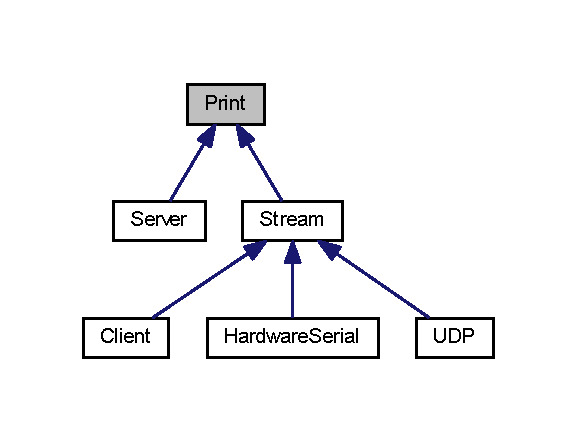
\includegraphics[width=277pt]{class_print__inherit__graph}
\end{center}
\end{figure}
\subsection*{Public Member Functions}
\begin{DoxyCompactItemize}
\item 
\hyperlink{class_print_aacaf064c16179a713ca892501f767628}{Print} ()
\item 
int \hyperlink{class_print_a207358e5283fd1720a123ed58ec79196}{get\+Write\+Error} ()
\item 
void \hyperlink{class_print_af50f0c1e1c726ef3dee08a84456090b9}{clear\+Write\+Error} ()
\item 
virtual size\+\_\+t \hyperlink{class_print_acde4db2f92186810af3493fd2c7535f0}{write} (uint8\+\_\+t)=0
\item 
size\+\_\+t \hyperlink{class_print_add50e5436017b9c2f1e0d11c9476bf1b}{write} (const char $\ast$str)
\item 
virtual size\+\_\+t \hyperlink{class_print_a7c66fc8d559f4956d4ccea196299bca7}{write} (const uint8\+\_\+t $\ast$buffer, size\+\_\+t size)
\item 
size\+\_\+t \hyperlink{class_print_ab81a6ce741d7baea3821248649bdeaca}{write} (const char $\ast$buffer, size\+\_\+t size)
\item 
size\+\_\+t \hyperlink{class_print_a443a13ae44e1a8930db53fc5161554f9}{print} (const \+\_\+\+\_\+\+Flash\+String\+Helper $\ast$)
\item 
size\+\_\+t \hyperlink{class_print_a2e9a01ff871af146cfbf2f321e60853f}{print} (const String \&)
\item 
size\+\_\+t \hyperlink{class_print_aae81a9f0e10656d079c8ee3d871f95dd}{print} (const char\mbox{[}$\,$\mbox{]})
\item 
size\+\_\+t \hyperlink{class_print_abd72fb37c98f21760aa7882cb34bf86b}{print} (char)
\item 
size\+\_\+t \hyperlink{class_print_a24bf7a9a27ae741994b38fbf45927a38}{print} (unsigned char, int=\hyperlink{_print_8h_afe38ec6126e35e40049e27fdf4586ba5}{D\+E\+C})
\item 
size\+\_\+t \hyperlink{class_print_ad485be2c2a9bd124789a58e41533bec3}{print} (int, int=\hyperlink{_print_8h_afe38ec6126e35e40049e27fdf4586ba5}{D\+E\+C})
\item 
size\+\_\+t \hyperlink{class_print_a5162c987fb51e1f223b92af3ed436d9c}{print} (unsigned int, int=\hyperlink{_print_8h_afe38ec6126e35e40049e27fdf4586ba5}{D\+E\+C})
\item 
size\+\_\+t \hyperlink{class_print_a447df1d390c7dc8af70f7e684963b212}{print} (long, int=\hyperlink{_print_8h_afe38ec6126e35e40049e27fdf4586ba5}{D\+E\+C})
\item 
size\+\_\+t \hyperlink{class_print_ae3b005981b3f34d0f352632204a52edf}{print} (unsigned long, int=\hyperlink{_print_8h_afe38ec6126e35e40049e27fdf4586ba5}{D\+E\+C})
\item 
size\+\_\+t \hyperlink{class_print_aa538defb056f77e8664a6ef29d281a8c}{print} (double, int=2)
\item 
size\+\_\+t \hyperlink{class_print_a922b3bb2a3e42c1b0c5b1d62b3a8fb3f}{print} (const \hyperlink{class_printable}{Printable} \&)
\item 
size\+\_\+t \hyperlink{class_print_a36d02f29121121bca22cd51d468dfa9e}{println} (const \+\_\+\+\_\+\+Flash\+String\+Helper $\ast$)
\item 
size\+\_\+t \hyperlink{class_print_a44007d63e31bec0bd3854eab1796c53d}{println} (const String \&s)
\item 
size\+\_\+t \hyperlink{class_print_abf944a191b3d93d87782824496fc9856}{println} (const char\mbox{[}$\,$\mbox{]})
\item 
size\+\_\+t \hyperlink{class_print_a6067829b7b76b5a541039c12ae1a9f7d}{println} (char)
\item 
size\+\_\+t \hyperlink{class_print_a0fb229c37a731c53ded8e9e832b4a0a6}{println} (unsigned char, int=\hyperlink{_print_8h_afe38ec6126e35e40049e27fdf4586ba5}{D\+E\+C})
\item 
size\+\_\+t \hyperlink{class_print_a058fbcd23e761e3d2fbe06bb1a07b737}{println} (int, int=\hyperlink{_print_8h_afe38ec6126e35e40049e27fdf4586ba5}{D\+E\+C})
\item 
size\+\_\+t \hyperlink{class_print_ac63f5e2c9a519af617af8880a4912ea7}{println} (unsigned int, int=\hyperlink{_print_8h_afe38ec6126e35e40049e27fdf4586ba5}{D\+E\+C})
\item 
size\+\_\+t \hyperlink{class_print_a173af0cd520b7105bcb2d63ab79d246f}{println} (long, int=\hyperlink{_print_8h_afe38ec6126e35e40049e27fdf4586ba5}{D\+E\+C})
\item 
size\+\_\+t \hyperlink{class_print_a74c918137834a92d0b82537e90d02ed5}{println} (unsigned long, int=\hyperlink{_print_8h_afe38ec6126e35e40049e27fdf4586ba5}{D\+E\+C})
\item 
size\+\_\+t \hyperlink{class_print_a2864f4a5017f1e2e2b8e46a8d185aab0}{println} (double, int=2)
\item 
size\+\_\+t \hyperlink{class_print_aec2662333be402d9f95f7e2a8bbf7202}{println} (const \hyperlink{class_printable}{Printable} \&)
\item 
size\+\_\+t \hyperlink{class_print_a7a21cd59cb8deef99051130e7852e382}{println} (void)
\end{DoxyCompactItemize}
\subsection*{Protected Member Functions}
\begin{DoxyCompactItemize}
\item 
void \hyperlink{class_print_ae0b8de12769dcf4c9b1fd3e67b3b7552}{set\+Write\+Error} (int err=1)
\end{DoxyCompactItemize}


\subsection{Detailed Description}


Definition at line 34 of file Print.\+h.



\subsection{Constructor \& Destructor Documentation}
\hypertarget{class_print_aacaf064c16179a713ca892501f767628}{}\index{Print@{Print}!Print@{Print}}
\index{Print@{Print}!Print@{Print}}
\subsubsection[{Print()}]{\setlength{\rightskip}{0pt plus 5cm}{\bf Print} (
\begin{DoxyParamCaption}
{}
\end{DoxyParamCaption}
)\hspace{0.3cm}{\ttfamily [inline]}}\label{class_print_aacaf064c16179a713ca892501f767628}


Definition at line 43 of file Print.\+h.



\subsection{Member Function Documentation}
\hypertarget{class_print_af50f0c1e1c726ef3dee08a84456090b9}{}\index{Print@{Print}!clear\+Write\+Error@{clear\+Write\+Error}}
\index{clear\+Write\+Error@{clear\+Write\+Error}!Print@{Print}}
\subsubsection[{clear\+Write\+Error()}]{\setlength{\rightskip}{0pt plus 5cm}void clear\+Write\+Error (
\begin{DoxyParamCaption}
{}
\end{DoxyParamCaption}
)\hspace{0.3cm}{\ttfamily [inline]}}\label{class_print_af50f0c1e1c726ef3dee08a84456090b9}


Definition at line 46 of file Print.\+h.



Here is the call graph for this function\+:
\nopagebreak
\begin{figure}[H]
\begin{center}
\leavevmode
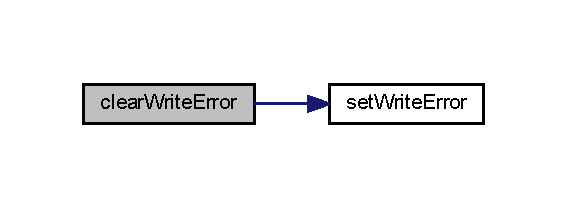
\includegraphics[width=272pt]{class_print_af50f0c1e1c726ef3dee08a84456090b9_cgraph}
\end{center}
\end{figure}


\hypertarget{class_print_a207358e5283fd1720a123ed58ec79196}{}\index{Print@{Print}!get\+Write\+Error@{get\+Write\+Error}}
\index{get\+Write\+Error@{get\+Write\+Error}!Print@{Print}}
\subsubsection[{get\+Write\+Error()}]{\setlength{\rightskip}{0pt plus 5cm}int get\+Write\+Error (
\begin{DoxyParamCaption}
{}
\end{DoxyParamCaption}
)\hspace{0.3cm}{\ttfamily [inline]}}\label{class_print_a207358e5283fd1720a123ed58ec79196}


Definition at line 45 of file Print.\+h.

\hypertarget{class_print_a443a13ae44e1a8930db53fc5161554f9}{}\index{Print@{Print}!print@{print}}
\index{print@{print}!Print@{Print}}
\subsubsection[{print(const \+\_\+\+\_\+\+Flash\+String\+Helper $\ast$)}]{\setlength{\rightskip}{0pt plus 5cm}size\+\_\+t print (
\begin{DoxyParamCaption}
\item[{const \+\_\+\+\_\+\+Flash\+String\+Helper $\ast$}]{ifsh}
\end{DoxyParamCaption}
)}\label{class_print_a443a13ae44e1a8930db53fc5161554f9}


Definition at line 42 of file Print.\+cpp.



Here is the call graph for this function\+:
\nopagebreak
\begin{figure}[H]
\begin{center}
\leavevmode
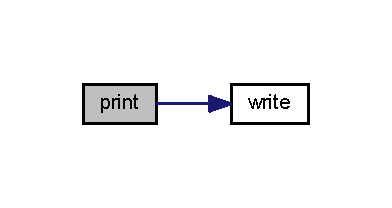
\includegraphics[width=188pt]{class_print_a443a13ae44e1a8930db53fc5161554f9_cgraph}
\end{center}
\end{figure}




Here is the caller graph for this function\+:
\nopagebreak
\begin{figure}[H]
\begin{center}
\leavevmode
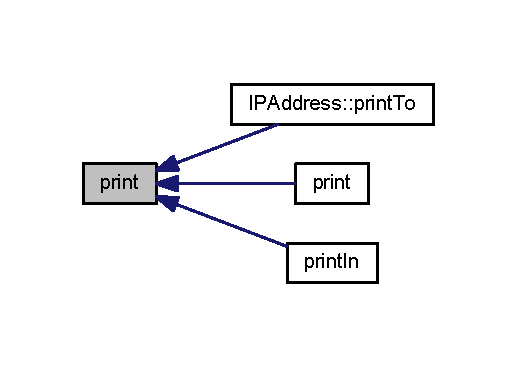
\includegraphics[width=248pt]{class_print_a443a13ae44e1a8930db53fc5161554f9_icgraph}
\end{center}
\end{figure}


\hypertarget{class_print_a2e9a01ff871af146cfbf2f321e60853f}{}\index{Print@{Print}!print@{print}}
\index{print@{print}!Print@{Print}}
\subsubsection[{print(const String \&)}]{\setlength{\rightskip}{0pt plus 5cm}size\+\_\+t print (
\begin{DoxyParamCaption}
\item[{const String \&}]{s}
\end{DoxyParamCaption}
)}\label{class_print_a2e9a01ff871af146cfbf2f321e60853f}


Definition at line 54 of file Print.\+cpp.



Here is the call graph for this function\+:
\nopagebreak
\begin{figure}[H]
\begin{center}
\leavevmode
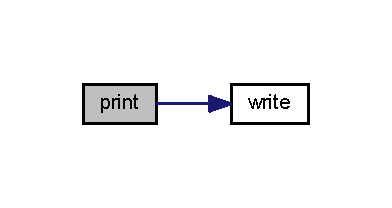
\includegraphics[width=188pt]{class_print_a2e9a01ff871af146cfbf2f321e60853f_cgraph}
\end{center}
\end{figure}


\hypertarget{class_print_aae81a9f0e10656d079c8ee3d871f95dd}{}\index{Print@{Print}!print@{print}}
\index{print@{print}!Print@{Print}}
\subsubsection[{print(const char[])}]{\setlength{\rightskip}{0pt plus 5cm}size\+\_\+t print (
\begin{DoxyParamCaption}
\item[{const char}]{str\mbox{[}$\,$\mbox{]}}
\end{DoxyParamCaption}
)}\label{class_print_aae81a9f0e10656d079c8ee3d871f95dd}


Definition at line 59 of file Print.\+cpp.



Here is the call graph for this function\+:
\nopagebreak
\begin{figure}[H]
\begin{center}
\leavevmode
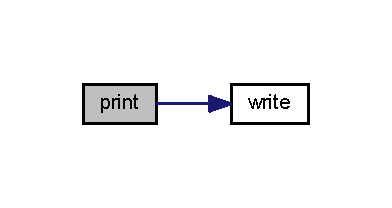
\includegraphics[width=188pt]{class_print_aae81a9f0e10656d079c8ee3d871f95dd_cgraph}
\end{center}
\end{figure}


\hypertarget{class_print_abd72fb37c98f21760aa7882cb34bf86b}{}\index{Print@{Print}!print@{print}}
\index{print@{print}!Print@{Print}}
\subsubsection[{print(char)}]{\setlength{\rightskip}{0pt plus 5cm}size\+\_\+t print (
\begin{DoxyParamCaption}
\item[{char}]{c}
\end{DoxyParamCaption}
)}\label{class_print_abd72fb37c98f21760aa7882cb34bf86b}


Definition at line 64 of file Print.\+cpp.



Here is the call graph for this function\+:
\nopagebreak
\begin{figure}[H]
\begin{center}
\leavevmode
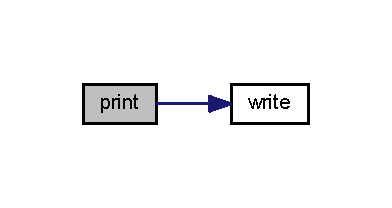
\includegraphics[width=188pt]{class_print_abd72fb37c98f21760aa7882cb34bf86b_cgraph}
\end{center}
\end{figure}


\hypertarget{class_print_a24bf7a9a27ae741994b38fbf45927a38}{}\index{Print@{Print}!print@{print}}
\index{print@{print}!Print@{Print}}
\subsubsection[{print(unsigned char, int=\+D\+E\+C)}]{\setlength{\rightskip}{0pt plus 5cm}size\+\_\+t print (
\begin{DoxyParamCaption}
\item[{unsigned char}]{b, }
\item[{int}]{base = {\ttfamily {\bf D\+E\+C}}}
\end{DoxyParamCaption}
)}\label{class_print_a24bf7a9a27ae741994b38fbf45927a38}


Definition at line 69 of file Print.\+cpp.



Here is the call graph for this function\+:
\nopagebreak
\begin{figure}[H]
\begin{center}
\leavevmode
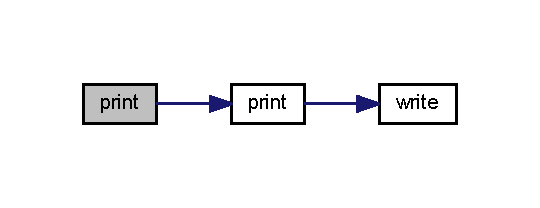
\includegraphics[width=259pt]{class_print_a24bf7a9a27ae741994b38fbf45927a38_cgraph}
\end{center}
\end{figure}


\hypertarget{class_print_ad485be2c2a9bd124789a58e41533bec3}{}\index{Print@{Print}!print@{print}}
\index{print@{print}!Print@{Print}}
\subsubsection[{print(int, int=\+D\+E\+C)}]{\setlength{\rightskip}{0pt plus 5cm}size\+\_\+t print (
\begin{DoxyParamCaption}
\item[{int}]{n, }
\item[{int}]{base = {\ttfamily {\bf D\+E\+C}}}
\end{DoxyParamCaption}
)}\label{class_print_ad485be2c2a9bd124789a58e41533bec3}


Definition at line 74 of file Print.\+cpp.



Here is the call graph for this function\+:
\nopagebreak
\begin{figure}[H]
\begin{center}
\leavevmode
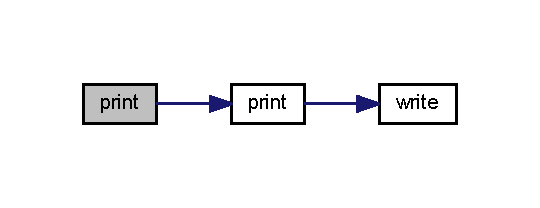
\includegraphics[width=259pt]{class_print_ad485be2c2a9bd124789a58e41533bec3_cgraph}
\end{center}
\end{figure}


\hypertarget{class_print_a5162c987fb51e1f223b92af3ed436d9c}{}\index{Print@{Print}!print@{print}}
\index{print@{print}!Print@{Print}}
\subsubsection[{print(unsigned int, int=\+D\+E\+C)}]{\setlength{\rightskip}{0pt plus 5cm}size\+\_\+t print (
\begin{DoxyParamCaption}
\item[{unsigned int}]{n, }
\item[{int}]{base = {\ttfamily {\bf D\+E\+C}}}
\end{DoxyParamCaption}
)}\label{class_print_a5162c987fb51e1f223b92af3ed436d9c}


Definition at line 79 of file Print.\+cpp.



Here is the call graph for this function\+:
\nopagebreak
\begin{figure}[H]
\begin{center}
\leavevmode
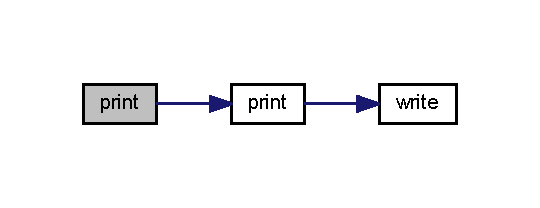
\includegraphics[width=259pt]{class_print_a5162c987fb51e1f223b92af3ed436d9c_cgraph}
\end{center}
\end{figure}


\hypertarget{class_print_a447df1d390c7dc8af70f7e684963b212}{}\index{Print@{Print}!print@{print}}
\index{print@{print}!Print@{Print}}
\subsubsection[{print(long, int=\+D\+E\+C)}]{\setlength{\rightskip}{0pt plus 5cm}size\+\_\+t print (
\begin{DoxyParamCaption}
\item[{long}]{n, }
\item[{int}]{base = {\ttfamily {\bf D\+E\+C}}}
\end{DoxyParamCaption}
)}\label{class_print_a447df1d390c7dc8af70f7e684963b212}


Definition at line 84 of file Print.\+cpp.



Here is the call graph for this function\+:
\nopagebreak
\begin{figure}[H]
\begin{center}
\leavevmode
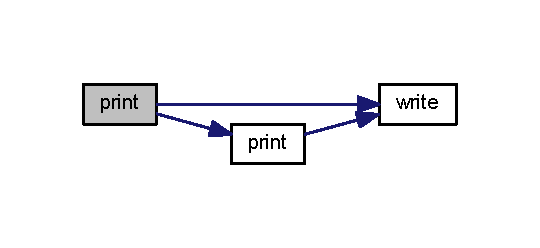
\includegraphics[width=259pt]{class_print_a447df1d390c7dc8af70f7e684963b212_cgraph}
\end{center}
\end{figure}


\hypertarget{class_print_ae3b005981b3f34d0f352632204a52edf}{}\index{Print@{Print}!print@{print}}
\index{print@{print}!Print@{Print}}
\subsubsection[{print(unsigned long, int=\+D\+E\+C)}]{\setlength{\rightskip}{0pt plus 5cm}size\+\_\+t print (
\begin{DoxyParamCaption}
\item[{unsigned long}]{n, }
\item[{int}]{base = {\ttfamily {\bf D\+E\+C}}}
\end{DoxyParamCaption}
)}\label{class_print_ae3b005981b3f34d0f352632204a52edf}


Definition at line 100 of file Print.\+cpp.



Here is the call graph for this function\+:
\nopagebreak
\begin{figure}[H]
\begin{center}
\leavevmode
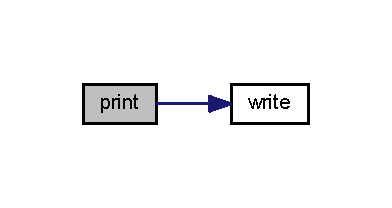
\includegraphics[width=188pt]{class_print_ae3b005981b3f34d0f352632204a52edf_cgraph}
\end{center}
\end{figure}


\hypertarget{class_print_aa538defb056f77e8664a6ef29d281a8c}{}\index{Print@{Print}!print@{print}}
\index{print@{print}!Print@{Print}}
\subsubsection[{print(double, int=2)}]{\setlength{\rightskip}{0pt plus 5cm}size\+\_\+t print (
\begin{DoxyParamCaption}
\item[{double}]{n, }
\item[{int}]{digits = {\ttfamily 2}}
\end{DoxyParamCaption}
)}\label{class_print_aa538defb056f77e8664a6ef29d281a8c}


Definition at line 106 of file Print.\+cpp.

\hypertarget{class_print_a922b3bb2a3e42c1b0c5b1d62b3a8fb3f}{}\index{Print@{Print}!print@{print}}
\index{print@{print}!Print@{Print}}
\subsubsection[{print(const Printable \&)}]{\setlength{\rightskip}{0pt plus 5cm}size\+\_\+t print (
\begin{DoxyParamCaption}
\item[{const {\bf Printable} \&}]{x}
\end{DoxyParamCaption}
)}\label{class_print_a922b3bb2a3e42c1b0c5b1d62b3a8fb3f}


Definition at line 118 of file Print.\+cpp.



Here is the call graph for this function\+:
\nopagebreak
\begin{figure}[H]
\begin{center}
\leavevmode
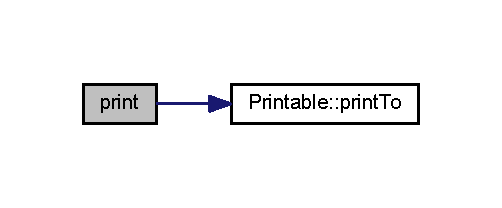
\includegraphics[width=241pt]{class_print_a922b3bb2a3e42c1b0c5b1d62b3a8fb3f_cgraph}
\end{center}
\end{figure}


\hypertarget{class_print_a36d02f29121121bca22cd51d468dfa9e}{}\index{Print@{Print}!println@{println}}
\index{println@{println}!Print@{Print}}
\subsubsection[{println(const \+\_\+\+\_\+\+Flash\+String\+Helper $\ast$)}]{\setlength{\rightskip}{0pt plus 5cm}size\+\_\+t println (
\begin{DoxyParamCaption}
\item[{const \+\_\+\+\_\+\+Flash\+String\+Helper $\ast$}]{ifsh}
\end{DoxyParamCaption}
)}\label{class_print_a36d02f29121121bca22cd51d468dfa9e}


Definition at line 111 of file Print.\+cpp.



Here is the call graph for this function\+:
\nopagebreak
\begin{figure}[H]
\begin{center}
\leavevmode
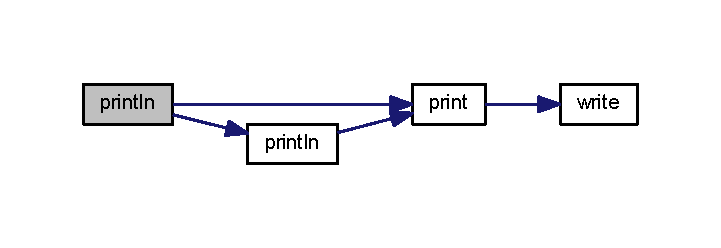
\includegraphics[width=346pt]{class_print_a36d02f29121121bca22cd51d468dfa9e_cgraph}
\end{center}
\end{figure}


\hypertarget{class_print_a44007d63e31bec0bd3854eab1796c53d}{}\index{Print@{Print}!println@{println}}
\index{println@{println}!Print@{Print}}
\subsubsection[{println(const String \&s)}]{\setlength{\rightskip}{0pt plus 5cm}size\+\_\+t println (
\begin{DoxyParamCaption}
\item[{const String \&}]{s}
\end{DoxyParamCaption}
)}\label{class_print_a44007d63e31bec0bd3854eab1796c53d}


Definition at line 130 of file Print.\+cpp.



Here is the call graph for this function\+:
\nopagebreak
\begin{figure}[H]
\begin{center}
\leavevmode
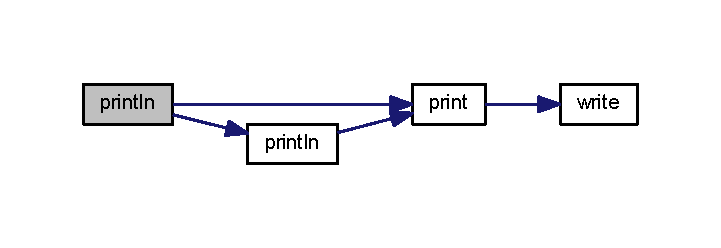
\includegraphics[width=346pt]{class_print_a44007d63e31bec0bd3854eab1796c53d_cgraph}
\end{center}
\end{figure}


\hypertarget{class_print_abf944a191b3d93d87782824496fc9856}{}\index{Print@{Print}!println@{println}}
\index{println@{println}!Print@{Print}}
\subsubsection[{println(const char[])}]{\setlength{\rightskip}{0pt plus 5cm}size\+\_\+t println (
\begin{DoxyParamCaption}
\item[{const char}]{c\mbox{[}$\,$\mbox{]}}
\end{DoxyParamCaption}
)}\label{class_print_abf944a191b3d93d87782824496fc9856}


Definition at line 137 of file Print.\+cpp.



Here is the call graph for this function\+:
\nopagebreak
\begin{figure}[H]
\begin{center}
\leavevmode
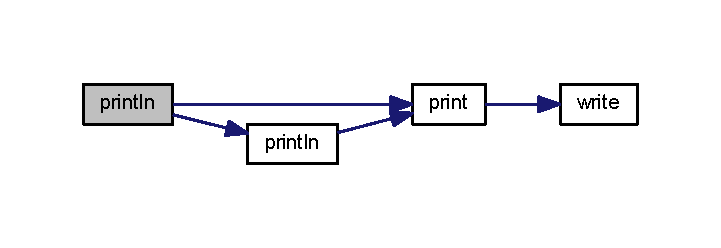
\includegraphics[width=346pt]{class_print_abf944a191b3d93d87782824496fc9856_cgraph}
\end{center}
\end{figure}


\hypertarget{class_print_a6067829b7b76b5a541039c12ae1a9f7d}{}\index{Print@{Print}!println@{println}}
\index{println@{println}!Print@{Print}}
\subsubsection[{println(char)}]{\setlength{\rightskip}{0pt plus 5cm}size\+\_\+t println (
\begin{DoxyParamCaption}
\item[{char}]{c}
\end{DoxyParamCaption}
)}\label{class_print_a6067829b7b76b5a541039c12ae1a9f7d}


Definition at line 144 of file Print.\+cpp.



Here is the call graph for this function\+:
\nopagebreak
\begin{figure}[H]
\begin{center}
\leavevmode
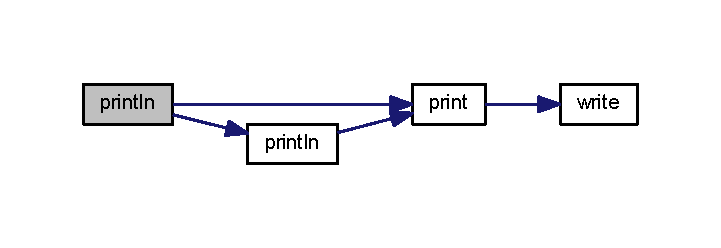
\includegraphics[width=346pt]{class_print_a6067829b7b76b5a541039c12ae1a9f7d_cgraph}
\end{center}
\end{figure}


\hypertarget{class_print_a0fb229c37a731c53ded8e9e832b4a0a6}{}\index{Print@{Print}!println@{println}}
\index{println@{println}!Print@{Print}}
\subsubsection[{println(unsigned char, int=\+D\+E\+C)}]{\setlength{\rightskip}{0pt plus 5cm}size\+\_\+t println (
\begin{DoxyParamCaption}
\item[{unsigned char}]{b, }
\item[{int}]{base = {\ttfamily {\bf D\+E\+C}}}
\end{DoxyParamCaption}
)}\label{class_print_a0fb229c37a731c53ded8e9e832b4a0a6}


Definition at line 151 of file Print.\+cpp.



Here is the call graph for this function\+:
\nopagebreak
\begin{figure}[H]
\begin{center}
\leavevmode
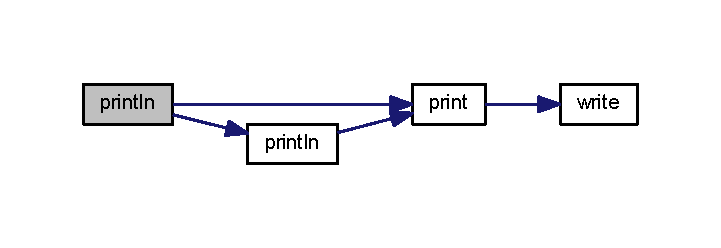
\includegraphics[width=346pt]{class_print_a0fb229c37a731c53ded8e9e832b4a0a6_cgraph}
\end{center}
\end{figure}


\hypertarget{class_print_a058fbcd23e761e3d2fbe06bb1a07b737}{}\index{Print@{Print}!println@{println}}
\index{println@{println}!Print@{Print}}
\subsubsection[{println(int, int=\+D\+E\+C)}]{\setlength{\rightskip}{0pt plus 5cm}size\+\_\+t println (
\begin{DoxyParamCaption}
\item[{int}]{num, }
\item[{int}]{base = {\ttfamily {\bf D\+E\+C}}}
\end{DoxyParamCaption}
)}\label{class_print_a058fbcd23e761e3d2fbe06bb1a07b737}


Definition at line 158 of file Print.\+cpp.



Here is the call graph for this function\+:
\nopagebreak
\begin{figure}[H]
\begin{center}
\leavevmode
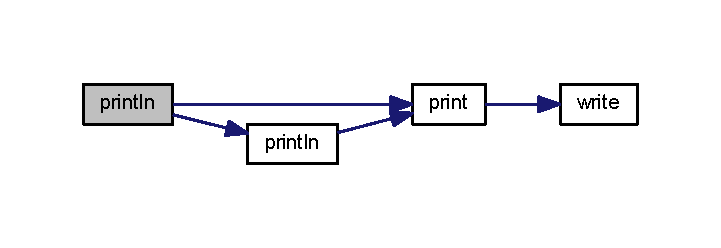
\includegraphics[width=346pt]{class_print_a058fbcd23e761e3d2fbe06bb1a07b737_cgraph}
\end{center}
\end{figure}


\hypertarget{class_print_ac63f5e2c9a519af617af8880a4912ea7}{}\index{Print@{Print}!println@{println}}
\index{println@{println}!Print@{Print}}
\subsubsection[{println(unsigned int, int=\+D\+E\+C)}]{\setlength{\rightskip}{0pt plus 5cm}size\+\_\+t println (
\begin{DoxyParamCaption}
\item[{unsigned int}]{num, }
\item[{int}]{base = {\ttfamily {\bf D\+E\+C}}}
\end{DoxyParamCaption}
)}\label{class_print_ac63f5e2c9a519af617af8880a4912ea7}


Definition at line 165 of file Print.\+cpp.



Here is the call graph for this function\+:
\nopagebreak
\begin{figure}[H]
\begin{center}
\leavevmode
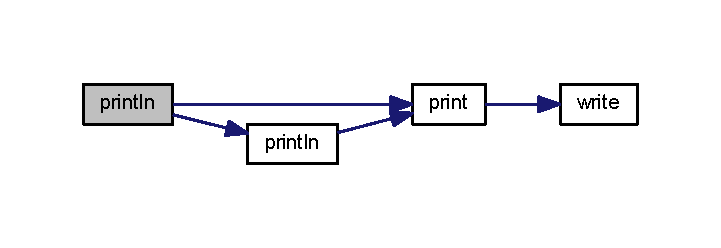
\includegraphics[width=346pt]{class_print_ac63f5e2c9a519af617af8880a4912ea7_cgraph}
\end{center}
\end{figure}


\hypertarget{class_print_a173af0cd520b7105bcb2d63ab79d246f}{}\index{Print@{Print}!println@{println}}
\index{println@{println}!Print@{Print}}
\subsubsection[{println(long, int=\+D\+E\+C)}]{\setlength{\rightskip}{0pt plus 5cm}size\+\_\+t println (
\begin{DoxyParamCaption}
\item[{long}]{num, }
\item[{int}]{base = {\ttfamily {\bf D\+E\+C}}}
\end{DoxyParamCaption}
)}\label{class_print_a173af0cd520b7105bcb2d63ab79d246f}


Definition at line 172 of file Print.\+cpp.



Here is the call graph for this function\+:
\nopagebreak
\begin{figure}[H]
\begin{center}
\leavevmode
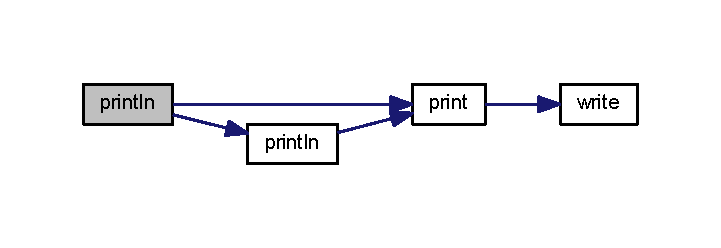
\includegraphics[width=346pt]{class_print_a173af0cd520b7105bcb2d63ab79d246f_cgraph}
\end{center}
\end{figure}


\hypertarget{class_print_a74c918137834a92d0b82537e90d02ed5}{}\index{Print@{Print}!println@{println}}
\index{println@{println}!Print@{Print}}
\subsubsection[{println(unsigned long, int=\+D\+E\+C)}]{\setlength{\rightskip}{0pt plus 5cm}size\+\_\+t println (
\begin{DoxyParamCaption}
\item[{unsigned long}]{num, }
\item[{int}]{base = {\ttfamily {\bf D\+E\+C}}}
\end{DoxyParamCaption}
)}\label{class_print_a74c918137834a92d0b82537e90d02ed5}


Definition at line 179 of file Print.\+cpp.



Here is the call graph for this function\+:
\nopagebreak
\begin{figure}[H]
\begin{center}
\leavevmode
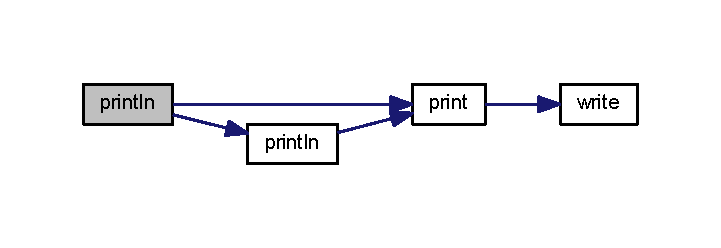
\includegraphics[width=346pt]{class_print_a74c918137834a92d0b82537e90d02ed5_cgraph}
\end{center}
\end{figure}


\hypertarget{class_print_a2864f4a5017f1e2e2b8e46a8d185aab0}{}\index{Print@{Print}!println@{println}}
\index{println@{println}!Print@{Print}}
\subsubsection[{println(double, int=2)}]{\setlength{\rightskip}{0pt plus 5cm}size\+\_\+t println (
\begin{DoxyParamCaption}
\item[{double}]{num, }
\item[{int}]{digits = {\ttfamily 2}}
\end{DoxyParamCaption}
)}\label{class_print_a2864f4a5017f1e2e2b8e46a8d185aab0}


Definition at line 186 of file Print.\+cpp.



Here is the call graph for this function\+:
\nopagebreak
\begin{figure}[H]
\begin{center}
\leavevmode
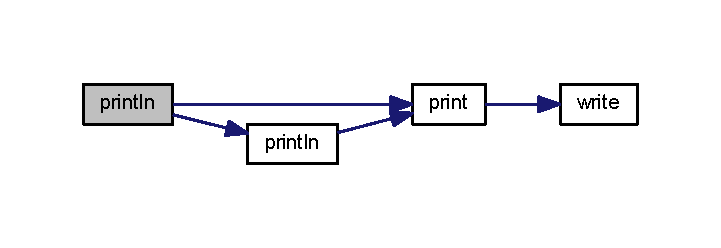
\includegraphics[width=346pt]{class_print_a2864f4a5017f1e2e2b8e46a8d185aab0_cgraph}
\end{center}
\end{figure}


\hypertarget{class_print_aec2662333be402d9f95f7e2a8bbf7202}{}\index{Print@{Print}!println@{println}}
\index{println@{println}!Print@{Print}}
\subsubsection[{println(const Printable \&)}]{\setlength{\rightskip}{0pt plus 5cm}size\+\_\+t println (
\begin{DoxyParamCaption}
\item[{const {\bf Printable} \&}]{x}
\end{DoxyParamCaption}
)}\label{class_print_aec2662333be402d9f95f7e2a8bbf7202}


Definition at line 193 of file Print.\+cpp.



Here is the call graph for this function\+:
\nopagebreak
\begin{figure}[H]
\begin{center}
\leavevmode
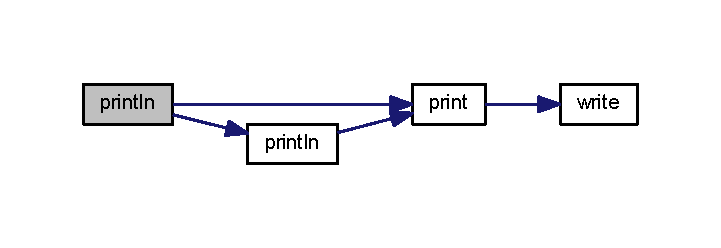
\includegraphics[width=346pt]{class_print_aec2662333be402d9f95f7e2a8bbf7202_cgraph}
\end{center}
\end{figure}


\hypertarget{class_print_a7a21cd59cb8deef99051130e7852e382}{}\index{Print@{Print}!println@{println}}
\index{println@{println}!Print@{Print}}
\subsubsection[{println(void)}]{\setlength{\rightskip}{0pt plus 5cm}size\+\_\+t println (
\begin{DoxyParamCaption}
\item[{void}]{}
\end{DoxyParamCaption}
)}\label{class_print_a7a21cd59cb8deef99051130e7852e382}


Definition at line 123 of file Print.\+cpp.



Here is the call graph for this function\+:
\nopagebreak
\begin{figure}[H]
\begin{center}
\leavevmode
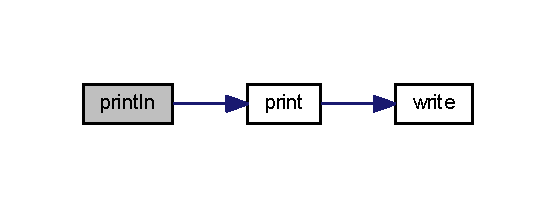
\includegraphics[width=267pt]{class_print_a7a21cd59cb8deef99051130e7852e382_cgraph}
\end{center}
\end{figure}




Here is the caller graph for this function\+:
\nopagebreak
\begin{figure}[H]
\begin{center}
\leavevmode
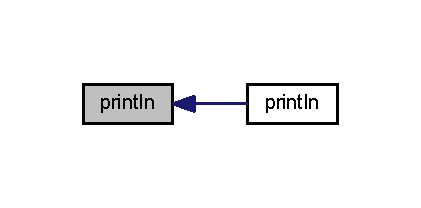
\includegraphics[width=202pt]{class_print_a7a21cd59cb8deef99051130e7852e382_icgraph}
\end{center}
\end{figure}


\hypertarget{class_print_ae0b8de12769dcf4c9b1fd3e67b3b7552}{}\index{Print@{Print}!set\+Write\+Error@{set\+Write\+Error}}
\index{set\+Write\+Error@{set\+Write\+Error}!Print@{Print}}
\subsubsection[{set\+Write\+Error(int err=1)}]{\setlength{\rightskip}{0pt plus 5cm}void set\+Write\+Error (
\begin{DoxyParamCaption}
\item[{int}]{err = {\ttfamily 1}}
\end{DoxyParamCaption}
)\hspace{0.3cm}{\ttfamily [inline]}, {\ttfamily [protected]}}\label{class_print_ae0b8de12769dcf4c9b1fd3e67b3b7552}


Definition at line 41 of file Print.\+h.



Here is the caller graph for this function\+:
\nopagebreak
\begin{figure}[H]
\begin{center}
\leavevmode
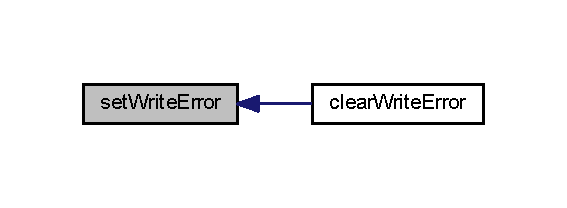
\includegraphics[width=272pt]{class_print_ae0b8de12769dcf4c9b1fd3e67b3b7552_icgraph}
\end{center}
\end{figure}


\hypertarget{class_print_acde4db2f92186810af3493fd2c7535f0}{}\index{Print@{Print}!write@{write}}
\index{write@{write}!Print@{Print}}
\subsubsection[{write(uint8\+\_\+t)=0}]{\setlength{\rightskip}{0pt plus 5cm}virtual size\+\_\+t write (
\begin{DoxyParamCaption}
\item[{uint8\+\_\+t}]{}
\end{DoxyParamCaption}
)\hspace{0.3cm}{\ttfamily [pure virtual]}}\label{class_print_acde4db2f92186810af3493fd2c7535f0}


Implemented in \hyperlink{class_hardware_serial_a0c15a57daf1517586523b8d270d34c7d}{Hardware\+Serial}, \hyperlink{class_u_d_p_acde4db2f92186810af3493fd2c7535f0}{U\+D\+P}, and \hyperlink{class_client_acde4db2f92186810af3493fd2c7535f0}{Client}.



Here is the caller graph for this function\+:
\nopagebreak
\begin{figure}[H]
\begin{center}
\leavevmode
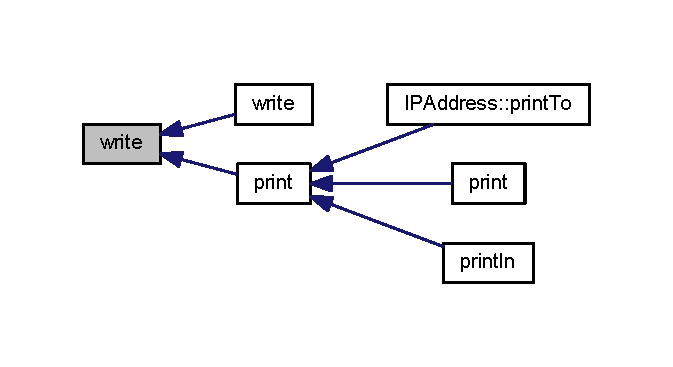
\includegraphics[width=323pt]{class_print_acde4db2f92186810af3493fd2c7535f0_icgraph}
\end{center}
\end{figure}


\hypertarget{class_print_add50e5436017b9c2f1e0d11c9476bf1b}{}\index{Print@{Print}!write@{write}}
\index{write@{write}!Print@{Print}}
\subsubsection[{write(const char $\ast$str)}]{\setlength{\rightskip}{0pt plus 5cm}size\+\_\+t write (
\begin{DoxyParamCaption}
\item[{const char $\ast$}]{str}
\end{DoxyParamCaption}
)\hspace{0.3cm}{\ttfamily [inline]}}\label{class_print_add50e5436017b9c2f1e0d11c9476bf1b}


Definition at line 49 of file Print.\+h.



Here is the call graph for this function\+:
\nopagebreak
\begin{figure}[H]
\begin{center}
\leavevmode
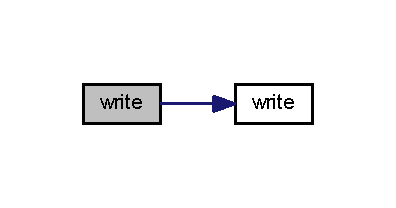
\includegraphics[width=190pt]{class_print_add50e5436017b9c2f1e0d11c9476bf1b_cgraph}
\end{center}
\end{figure}


\hypertarget{class_print_a7c66fc8d559f4956d4ccea196299bca7}{}\index{Print@{Print}!write@{write}}
\index{write@{write}!Print@{Print}}
\subsubsection[{write(const uint8\+\_\+t $\ast$buffer, size\+\_\+t size)}]{\setlength{\rightskip}{0pt plus 5cm}size\+\_\+t write (
\begin{DoxyParamCaption}
\item[{const uint8\+\_\+t $\ast$}]{buffer, }
\item[{size\+\_\+t}]{size}
\end{DoxyParamCaption}
)\hspace{0.3cm}{\ttfamily [virtual]}}\label{class_print_a7c66fc8d559f4956d4ccea196299bca7}


Reimplemented in \hyperlink{class_u_d_p_acd93fd9e345711179a5a2af3d46b8b81}{U\+D\+P}, and \hyperlink{class_client_a7565f7448952b08e42489b3162638f69}{Client}.



Definition at line 33 of file Print.\+cpp.



Here is the call graph for this function\+:
\nopagebreak
\begin{figure}[H]
\begin{center}
\leavevmode
\includegraphics[width=190pt]{class_print_a7c66fc8d559f4956d4ccea196299bca7_cgraph}
\end{center}
\end{figure}


\hypertarget{class_print_ab81a6ce741d7baea3821248649bdeaca}{}\index{Print@{Print}!write@{write}}
\index{write@{write}!Print@{Print}}
\subsubsection[{write(const char $\ast$buffer, size\+\_\+t size)}]{\setlength{\rightskip}{0pt plus 5cm}size\+\_\+t write (
\begin{DoxyParamCaption}
\item[{const char $\ast$}]{buffer, }
\item[{size\+\_\+t}]{size}
\end{DoxyParamCaption}
)\hspace{0.3cm}{\ttfamily [inline]}}\label{class_print_ab81a6ce741d7baea3821248649bdeaca}


Definition at line 54 of file Print.\+h.



Here is the call graph for this function\+:
\nopagebreak
\begin{figure}[H]
\begin{center}
\leavevmode
\includegraphics[width=190pt]{class_print_ab81a6ce741d7baea3821248649bdeaca_cgraph}
\end{center}
\end{figure}




The documentation for this class was generated from the following files\+:\begin{DoxyCompactItemize}
\item 
Arduino\+U\+N\+O/src/arduino/cores/arduino/\hyperlink{_print_8h}{Print.\+h}\item 
Arduino\+U\+N\+O/src/arduino/cores/arduino/\hyperlink{_print_8cpp}{Print.\+cpp}\end{DoxyCompactItemize}

\hypertarget{class_printable}{}\section{Printable Class Reference}
\label{class_printable}\index{Printable@{Printable}}


{\ttfamily \#include $<$Printable.\+h$>$}



Inheritance diagram for Printable\+:
\nopagebreak
\begin{figure}[H]
\begin{center}
\leavevmode
\includegraphics[width=142pt]{class_printable__inherit__graph}
\end{center}
\end{figure}
\subsection*{Public Member Functions}
\begin{DoxyCompactItemize}
\item 
virtual size\+\_\+t \hyperlink{class_printable_a95c9f86bb3e38a8743433c80c9250664}{print\+To} (\hyperlink{class_print}{Print} \&p) const  =0
\end{DoxyCompactItemize}


\subsection{Detailed Description}
The \hyperlink{class_printable}{Printable} class provides a way for new classes to allow themselves to be printed. By deriving from \hyperlink{class_printable}{Printable} and implementing the print\+To method, it will then be possible for users to print out instances of this class by passing them into the usual \hyperlink{class_print_a443a13ae44e1a8930db53fc5161554f9}{Print\+::print} and \hyperlink{class_print_a36d02f29121121bca22cd51d468dfa9e}{Print\+::println} methods. 

Definition at line 33 of file Printable.\+h.



\subsection{Member Function Documentation}
\hypertarget{class_printable_a95c9f86bb3e38a8743433c80c9250664}{}\index{Printable@{Printable}!print\+To@{print\+To}}
\index{print\+To@{print\+To}!Printable@{Printable}}
\subsubsection[{print\+To(\+Print \&p) const  =0}]{\setlength{\rightskip}{0pt plus 5cm}virtual size\+\_\+t print\+To (
\begin{DoxyParamCaption}
\item[{{\bf Print} \&}]{p}
\end{DoxyParamCaption}
) const\hspace{0.3cm}{\ttfamily [pure virtual]}}\label{class_printable_a95c9f86bb3e38a8743433c80c9250664}


Implemented in \hyperlink{class_i_p_address_a4de4b3920775530f38f756b2177a9bca}{I\+P\+Address}.



Here is the caller graph for this function\+:
\nopagebreak
\begin{figure}[H]
\begin{center}
\leavevmode
\includegraphics[width=224pt]{class_printable_a95c9f86bb3e38a8743433c80c9250664_icgraph}
\end{center}
\end{figure}




The documentation for this class was generated from the following file\+:\begin{DoxyCompactItemize}
\item 
Arduino\+U\+N\+O/src/arduino/cores/arduino/\hyperlink{_printable_8h}{Printable.\+h}\end{DoxyCompactItemize}

\hypertarget{class_server}{}\section{Server Class Reference}
\label{class_server}\index{Server@{Server}}


{\ttfamily \#include $<$Server.\+h$>$}



Inheritance diagram for Server\+:\nopagebreak
\begin{figure}[H]
\begin{center}
\leavevmode
\includegraphics[width=124pt]{class_server__inherit__graph}
\end{center}
\end{figure}


Collaboration diagram for Server\+:\nopagebreak
\begin{figure}[H]
\begin{center}
\leavevmode
\includegraphics[width=124pt]{class_server__coll__graph}
\end{center}
\end{figure}
\subsection*{Public Member Functions}
\begin{DoxyCompactItemize}
\item 
virtual void \hyperlink{class_server_aaf893c33f3c041e289a12c153dcc9789}{begin} ()=0
\end{DoxyCompactItemize}
\subsection*{Additional Inherited Members}


\subsection{Detailed Description}


Definition at line 25 of file Server.\+h.



\subsection{Member Function Documentation}
\hypertarget{class_server_aaf893c33f3c041e289a12c153dcc9789}{}\index{Server@{Server}!begin@{begin}}
\index{begin@{begin}!Server@{Server}}
\subsubsection[{begin()=0}]{\setlength{\rightskip}{0pt plus 5cm}virtual void begin (
\begin{DoxyParamCaption}
{}
\end{DoxyParamCaption}
)\hspace{0.3cm}{\ttfamily [pure virtual]}}\label{class_server_aaf893c33f3c041e289a12c153dcc9789}


The documentation for this class was generated from the following file\+:\begin{DoxyCompactItemize}
\item 
Arduino\+U\+N\+O/src/arduino/cores/arduino/\hyperlink{_server_8h}{Server.\+h}\end{DoxyCompactItemize}

\hypertarget{class_stream}{}\section{Stream Class Reference}
\label{class_stream}\index{Stream@{Stream}}


{\ttfamily \#include $<$Stream.\+h$>$}



Inheritance diagram for Stream\+:
\nopagebreak
\begin{figure}[H]
\begin{center}
\leavevmode
\includegraphics[width=277pt]{class_stream__inherit__graph}
\end{center}
\end{figure}


Collaboration diagram for Stream\+:
\nopagebreak
\begin{figure}[H]
\begin{center}
\leavevmode
\includegraphics[width=128pt]{class_stream__coll__graph}
\end{center}
\end{figure}
\subsection*{Data Structures}
\begin{DoxyCompactItemize}
\item 
struct \hyperlink{struct_stream_1_1_multi_target}{Multi\+Target}
\end{DoxyCompactItemize}
\subsection*{Public Member Functions}
\begin{DoxyCompactItemize}
\item 
virtual int \hyperlink{class_stream_aebd60457902debb30b07971a16f24ebd}{available} ()=0
\item 
virtual int \hyperlink{class_stream_a4afd50731ba321d1b9be909cb288a50b}{read} ()=0
\item 
virtual int \hyperlink{class_stream_a9ae768d427519818aa552adf467bf65a}{peek} ()=0
\item 
virtual void \hyperlink{class_stream_a50ab71f4bc571f6e246b20db4b3dd131}{flush} ()=0
\item 
\hyperlink{class_stream_a7411b49ed5fda5181dd182d64984906e}{Stream} ()
\item 
void \hyperlink{class_stream_a76c7d6530b9cb17f6663a64aea84b61e}{set\+Timeout} (unsigned long timeout)
\item 
bool \hyperlink{class_stream_a13fd59f691f095fc014b4c012cbd79f7}{find} (char $\ast$target)
\item 
bool \hyperlink{class_stream_a4b392ebdbb1b1eb5fb0b23cb3798ce04}{find} (uint8\+\_\+t $\ast$target)
\item 
bool \hyperlink{class_stream_a064fe7239eb0cc6ba4a41d064d90a51f}{find} (char $\ast$target, size\+\_\+t length)
\item 
bool \hyperlink{class_stream_acf54fbb26d6831374a6667b5a3201f22}{find} (uint8\+\_\+t $\ast$target, size\+\_\+t length)
\item 
bool \hyperlink{class_stream_ae9bf806705b80571316623814e5cb2ca}{find\+Until} (char $\ast$target, char $\ast$terminator)
\item 
bool \hyperlink{class_stream_a2cb0079bcfbffff6273404c8afaa4660}{find\+Until} (uint8\+\_\+t $\ast$target, char $\ast$terminator)
\item 
bool \hyperlink{class_stream_a99d1b6ad00abb9264b5ebb7506585993}{find\+Until} (char $\ast$target, size\+\_\+t target\+Len, char $\ast$terminate, size\+\_\+t term\+Len)
\item 
bool \hyperlink{class_stream_a5a3dbacf38766d57c845d6530f9aa109}{find\+Until} (uint8\+\_\+t $\ast$target, size\+\_\+t target\+Len, char $\ast$terminate, size\+\_\+t term\+Len)
\item 
long \hyperlink{class_stream_a4d54d18e24a5aff0faa15f40be995edf}{parse\+Int} ()
\item 
float \hyperlink{class_stream_a327a9ae2bfcaf84ddd69477839507ca7}{parse\+Float} ()
\item 
size\+\_\+t \hyperlink{class_stream_ada0b9486ea1fe7b8d4aab8f04f5607ee}{read\+Bytes} (char $\ast$buffer, size\+\_\+t length)
\item 
size\+\_\+t \hyperlink{class_stream_a4ef72b9bae2f35c08ddc4292e5ac1df4}{read\+Bytes} (uint8\+\_\+t $\ast$buffer, size\+\_\+t length)
\item 
size\+\_\+t \hyperlink{class_stream_a9aa68dc2abab64ceafe8d8745b728af2}{read\+Bytes\+Until} (char terminator, char $\ast$buffer, size\+\_\+t length)
\item 
size\+\_\+t \hyperlink{class_stream_a9fcaea3bb67432821ddbde8a13331429}{read\+Bytes\+Until} (char terminator, uint8\+\_\+t $\ast$buffer, size\+\_\+t length)
\item 
String \hyperlink{class_stream_ab1b0d4ef00718d18fe34d35dd1e26c66}{read\+String} ()
\item 
String \hyperlink{class_stream_ac1f2b6e32ae2e321ad98c16482edf96a}{read\+String\+Until} (char terminator)
\end{DoxyCompactItemize}
\subsection*{Protected Member Functions}
\begin{DoxyCompactItemize}
\item 
int \hyperlink{class_stream_a7cc09dd787a79c17281039b4456dc6aa}{timed\+Read} ()
\item 
int \hyperlink{class_stream_a157762e7d29562248c38ecbe6daa2fae}{timed\+Peek} ()
\item 
int \hyperlink{class_stream_a6a68a089460a8e332fad1002d36374a5}{peek\+Next\+Digit} ()
\item 
long \hyperlink{class_stream_aa5269d83a12f784ac9d54e19104d39fe}{parse\+Int} (char skip\+Char)
\item 
float \hyperlink{class_stream_aa66300bfdb6b2eda158d84dbaf5adcb5}{parse\+Float} (char skip\+Char)
\item 
int \hyperlink{class_stream_a34d087eec23d221a8ed4c5279cf9cf4c}{find\+Multi} (struct \hyperlink{struct_stream_1_1_multi_target}{Multi\+Target} $\ast$targets, int t\+Count)
\end{DoxyCompactItemize}
\subsection*{Protected Attributes}
\begin{DoxyCompactItemize}
\item 
unsigned long \hyperlink{class_stream_a24c7e4b09282e8150935ce8da759e176}{\+\_\+timeout}
\item 
unsigned long \hyperlink{class_stream_a30515d765ff208be483b71592aa9da72}{\+\_\+start\+Millis}
\end{DoxyCompactItemize}


\subsection{Detailed Description}


Definition at line 38 of file Stream.\+h.



\subsection{Constructor \& Destructor Documentation}
\hypertarget{class_stream_a7411b49ed5fda5181dd182d64984906e}{}\index{Stream@{Stream}!Stream@{Stream}}
\index{Stream@{Stream}!Stream@{Stream}}
\subsubsection[{Stream()}]{\setlength{\rightskip}{0pt plus 5cm}{\bf Stream} (
\begin{DoxyParamCaption}
{}
\end{DoxyParamCaption}
)\hspace{0.3cm}{\ttfamily [inline]}}\label{class_stream_a7411b49ed5fda5181dd182d64984906e}


Definition at line 53 of file Stream.\+h.



\subsection{Member Function Documentation}
\hypertarget{class_stream_aebd60457902debb30b07971a16f24ebd}{}\index{Stream@{Stream}!available@{available}}
\index{available@{available}!Stream@{Stream}}
\subsubsection[{available()=0}]{\setlength{\rightskip}{0pt plus 5cm}virtual int available (
\begin{DoxyParamCaption}
{}
\end{DoxyParamCaption}
)\hspace{0.3cm}{\ttfamily [pure virtual]}}\label{class_stream_aebd60457902debb30b07971a16f24ebd}


Implemented in \hyperlink{class_hardware_serial_aeec8f4dbef97221a6041d6cdc6e9b716}{Hardware\+Serial}, \hyperlink{class_u_d_p_aebd60457902debb30b07971a16f24ebd}{U\+D\+P}, and \hyperlink{class_client_aebd60457902debb30b07971a16f24ebd}{Client}.

\hypertarget{class_stream_a13fd59f691f095fc014b4c012cbd79f7}{}\index{Stream@{Stream}!find@{find}}
\index{find@{find}!Stream@{Stream}}
\subsubsection[{find(char $\ast$target)}]{\setlength{\rightskip}{0pt plus 5cm}bool find (
\begin{DoxyParamCaption}
\item[{char $\ast$}]{target}
\end{DoxyParamCaption}
)}\label{class_stream_a13fd59f691f095fc014b4c012cbd79f7}


Definition at line 78 of file Stream.\+cpp.



Here is the call graph for this function\+:
\nopagebreak
\begin{figure}[H]
\begin{center}
\leavevmode
\includegraphics[width=199pt]{class_stream_a13fd59f691f095fc014b4c012cbd79f7_cgraph}
\end{center}
\end{figure}


\hypertarget{class_stream_a4b392ebdbb1b1eb5fb0b23cb3798ce04}{}\index{Stream@{Stream}!find@{find}}
\index{find@{find}!Stream@{Stream}}
\subsubsection[{find(uint8\+\_\+t $\ast$target)}]{\setlength{\rightskip}{0pt plus 5cm}bool find (
\begin{DoxyParamCaption}
\item[{uint8\+\_\+t $\ast$}]{target}
\end{DoxyParamCaption}
)\hspace{0.3cm}{\ttfamily [inline]}}\label{class_stream_a4b392ebdbb1b1eb5fb0b23cb3798ce04}


Definition at line 60 of file Stream.\+h.



Here is the call graph for this function\+:
\nopagebreak
\begin{figure}[H]
\begin{center}
\leavevmode
\includegraphics[width=112pt]{class_stream_a4b392ebdbb1b1eb5fb0b23cb3798ce04_cgraph}
\end{center}
\end{figure}




Here is the caller graph for this function\+:
\nopagebreak
\begin{figure}[H]
\begin{center}
\leavevmode
\includegraphics[width=112pt]{class_stream_a4b392ebdbb1b1eb5fb0b23cb3798ce04_icgraph}
\end{center}
\end{figure}


\hypertarget{class_stream_a064fe7239eb0cc6ba4a41d064d90a51f}{}\index{Stream@{Stream}!find@{find}}
\index{find@{find}!Stream@{Stream}}
\subsubsection[{find(char $\ast$target, size\+\_\+t length)}]{\setlength{\rightskip}{0pt plus 5cm}bool find (
\begin{DoxyParamCaption}
\item[{char $\ast$}]{target, }
\item[{size\+\_\+t}]{length}
\end{DoxyParamCaption}
)}\label{class_stream_a064fe7239eb0cc6ba4a41d064d90a51f}


Definition at line 85 of file Stream.\+cpp.



Here is the call graph for this function\+:
\nopagebreak
\begin{figure}[H]
\begin{center}
\leavevmode
\includegraphics[width=199pt]{class_stream_a064fe7239eb0cc6ba4a41d064d90a51f_cgraph}
\end{center}
\end{figure}


\hypertarget{class_stream_acf54fbb26d6831374a6667b5a3201f22}{}\index{Stream@{Stream}!find@{find}}
\index{find@{find}!Stream@{Stream}}
\subsubsection[{find(uint8\+\_\+t $\ast$target, size\+\_\+t length)}]{\setlength{\rightskip}{0pt plus 5cm}bool find (
\begin{DoxyParamCaption}
\item[{uint8\+\_\+t $\ast$}]{target, }
\item[{size\+\_\+t}]{length}
\end{DoxyParamCaption}
)\hspace{0.3cm}{\ttfamily [inline]}}\label{class_stream_acf54fbb26d6831374a6667b5a3201f22}


Definition at line 64 of file Stream.\+h.



Here is the call graph for this function\+:
\nopagebreak
\begin{figure}[H]
\begin{center}
\leavevmode
\includegraphics[width=112pt]{class_stream_acf54fbb26d6831374a6667b5a3201f22_cgraph}
\end{center}
\end{figure}




Here is the caller graph for this function\+:
\nopagebreak
\begin{figure}[H]
\begin{center}
\leavevmode
\includegraphics[width=112pt]{class_stream_acf54fbb26d6831374a6667b5a3201f22_icgraph}
\end{center}
\end{figure}


\hypertarget{class_stream_a34d087eec23d221a8ed4c5279cf9cf4c}{}\index{Stream@{Stream}!find\+Multi@{find\+Multi}}
\index{find\+Multi@{find\+Multi}!Stream@{Stream}}
\subsubsection[{find\+Multi(struct Multi\+Target $\ast$targets, int t\+Count)}]{\setlength{\rightskip}{0pt plus 5cm}int find\+Multi (
\begin{DoxyParamCaption}
\item[{struct {\bf Multi\+Target} $\ast$}]{targets, }
\item[{int}]{t\+Count}
\end{DoxyParamCaption}
)\hspace{0.3cm}{\ttfamily [protected]}}\label{class_stream_a34d087eec23d221a8ed4c5279cf9cf4c}


Definition at line 254 of file Stream.\+cpp.



Here is the call graph for this function\+:
\nopagebreak
\begin{figure}[H]
\begin{center}
\leavevmode
\includegraphics[width=307pt]{class_stream_a34d087eec23d221a8ed4c5279cf9cf4c_cgraph}
\end{center}
\end{figure}




Here is the caller graph for this function\+:
\nopagebreak
\begin{figure}[H]
\begin{center}
\leavevmode
\includegraphics[width=220pt]{class_stream_a34d087eec23d221a8ed4c5279cf9cf4c_icgraph}
\end{center}
\end{figure}


\hypertarget{class_stream_ae9bf806705b80571316623814e5cb2ca}{}\index{Stream@{Stream}!find\+Until@{find\+Until}}
\index{find\+Until@{find\+Until}!Stream@{Stream}}
\subsubsection[{find\+Until(char $\ast$target, char $\ast$terminator)}]{\setlength{\rightskip}{0pt plus 5cm}bool find\+Until (
\begin{DoxyParamCaption}
\item[{char $\ast$}]{target, }
\item[{char $\ast$}]{terminator}
\end{DoxyParamCaption}
)}\label{class_stream_ae9bf806705b80571316623814e5cb2ca}


Definition at line 91 of file Stream.\+cpp.



Here is the caller graph for this function\+:
\nopagebreak
\begin{figure}[H]
\begin{center}
\leavevmode
\includegraphics[width=199pt]{class_stream_ae9bf806705b80571316623814e5cb2ca_icgraph}
\end{center}
\end{figure}


\hypertarget{class_stream_a2cb0079bcfbffff6273404c8afaa4660}{}\index{Stream@{Stream}!find\+Until@{find\+Until}}
\index{find\+Until@{find\+Until}!Stream@{Stream}}
\subsubsection[{find\+Until(uint8\+\_\+t $\ast$target, char $\ast$terminator)}]{\setlength{\rightskip}{0pt plus 5cm}bool find\+Until (
\begin{DoxyParamCaption}
\item[{uint8\+\_\+t $\ast$}]{target, }
\item[{char $\ast$}]{terminator}
\end{DoxyParamCaption}
)\hspace{0.3cm}{\ttfamily [inline]}}\label{class_stream_a2cb0079bcfbffff6273404c8afaa4660}


Definition at line 68 of file Stream.\+h.



Here is the call graph for this function\+:
\nopagebreak
\begin{figure}[H]
\begin{center}
\leavevmode
\includegraphics[width=131pt]{class_stream_a2cb0079bcfbffff6273404c8afaa4660_cgraph}
\end{center}
\end{figure}




Here is the caller graph for this function\+:
\nopagebreak
\begin{figure}[H]
\begin{center}
\leavevmode
\includegraphics[width=131pt]{class_stream_a2cb0079bcfbffff6273404c8afaa4660_icgraph}
\end{center}
\end{figure}


\hypertarget{class_stream_a99d1b6ad00abb9264b5ebb7506585993}{}\index{Stream@{Stream}!find\+Until@{find\+Until}}
\index{find\+Until@{find\+Until}!Stream@{Stream}}
\subsubsection[{find\+Until(char $\ast$target, size\+\_\+t target\+Len, char $\ast$terminate, size\+\_\+t term\+Len)}]{\setlength{\rightskip}{0pt plus 5cm}bool find\+Until (
\begin{DoxyParamCaption}
\item[{char $\ast$}]{target, }
\item[{size\+\_\+t}]{target\+Len, }
\item[{char $\ast$}]{terminate, }
\item[{size\+\_\+t}]{term\+Len}
\end{DoxyParamCaption}
)}\label{class_stream_a99d1b6ad00abb9264b5ebb7506585993}


Definition at line 99 of file Stream.\+cpp.



Here is the call graph for this function\+:
\nopagebreak
\begin{figure}[H]
\begin{center}
\leavevmode
\includegraphics[width=350pt]{class_stream_a99d1b6ad00abb9264b5ebb7506585993_cgraph}
\end{center}
\end{figure}


\hypertarget{class_stream_a5a3dbacf38766d57c845d6530f9aa109}{}\index{Stream@{Stream}!find\+Until@{find\+Until}}
\index{find\+Until@{find\+Until}!Stream@{Stream}}
\subsubsection[{find\+Until(uint8\+\_\+t $\ast$target, size\+\_\+t target\+Len, char $\ast$terminate, size\+\_\+t term\+Len)}]{\setlength{\rightskip}{0pt plus 5cm}bool find\+Until (
\begin{DoxyParamCaption}
\item[{uint8\+\_\+t $\ast$}]{target, }
\item[{size\+\_\+t}]{target\+Len, }
\item[{char $\ast$}]{terminate, }
\item[{size\+\_\+t}]{term\+Len}
\end{DoxyParamCaption}
)\hspace{0.3cm}{\ttfamily [inline]}}\label{class_stream_a5a3dbacf38766d57c845d6530f9aa109}


Definition at line 71 of file Stream.\+h.



Here is the call graph for this function\+:
\nopagebreak
\begin{figure}[H]
\begin{center}
\leavevmode
\includegraphics[width=131pt]{class_stream_a5a3dbacf38766d57c845d6530f9aa109_cgraph}
\end{center}
\end{figure}




Here is the caller graph for this function\+:
\nopagebreak
\begin{figure}[H]
\begin{center}
\leavevmode
\includegraphics[width=131pt]{class_stream_a5a3dbacf38766d57c845d6530f9aa109_icgraph}
\end{center}
\end{figure}


\hypertarget{class_stream_a50ab71f4bc571f6e246b20db4b3dd131}{}\index{Stream@{Stream}!flush@{flush}}
\index{flush@{flush}!Stream@{Stream}}
\subsubsection[{flush()=0}]{\setlength{\rightskip}{0pt plus 5cm}virtual void flush (
\begin{DoxyParamCaption}
{}
\end{DoxyParamCaption}
)\hspace{0.3cm}{\ttfamily [pure virtual]}}\label{class_stream_a50ab71f4bc571f6e246b20db4b3dd131}


Implemented in \hyperlink{class_hardware_serial_a0a4efd3d0f68d057f23eb5dfcd16c17c}{Hardware\+Serial}, \hyperlink{class_u_d_p_a50ab71f4bc571f6e246b20db4b3dd131}{U\+D\+P}, and \hyperlink{class_client_a50ab71f4bc571f6e246b20db4b3dd131}{Client}.

\hypertarget{class_stream_a327a9ae2bfcaf84ddd69477839507ca7}{}\index{Stream@{Stream}!parse\+Float@{parse\+Float}}
\index{parse\+Float@{parse\+Float}!Stream@{Stream}}
\subsubsection[{parse\+Float()}]{\setlength{\rightskip}{0pt plus 5cm}float parse\+Float (
\begin{DoxyParamCaption}
{}
\end{DoxyParamCaption}
)}\label{class_stream_a327a9ae2bfcaf84ddd69477839507ca7}


Definition at line 151 of file Stream.\+cpp.

\hypertarget{class_stream_aa66300bfdb6b2eda158d84dbaf5adcb5}{}\index{Stream@{Stream}!parse\+Float@{parse\+Float}}
\index{parse\+Float@{parse\+Float}!Stream@{Stream}}
\subsubsection[{parse\+Float(char skip\+Char)}]{\setlength{\rightskip}{0pt plus 5cm}float parse\+Float (
\begin{DoxyParamCaption}
\item[{char}]{skip\+Char}
\end{DoxyParamCaption}
)\hspace{0.3cm}{\ttfamily [protected]}}\label{class_stream_aa66300bfdb6b2eda158d84dbaf5adcb5}


Definition at line 158 of file Stream.\+cpp.



Here is the call graph for this function\+:
\nopagebreak
\begin{figure}[H]
\begin{center}
\leavevmode
\includegraphics[width=350pt]{class_stream_aa66300bfdb6b2eda158d84dbaf5adcb5_cgraph}
\end{center}
\end{figure}


\hypertarget{class_stream_a4d54d18e24a5aff0faa15f40be995edf}{}\index{Stream@{Stream}!parse\+Int@{parse\+Int}}
\index{parse\+Int@{parse\+Int}!Stream@{Stream}}
\subsubsection[{parse\+Int()}]{\setlength{\rightskip}{0pt plus 5cm}long parse\+Int (
\begin{DoxyParamCaption}
{}
\end{DoxyParamCaption}
)}\label{class_stream_a4d54d18e24a5aff0faa15f40be995edf}


Definition at line 114 of file Stream.\+cpp.

\hypertarget{class_stream_aa5269d83a12f784ac9d54e19104d39fe}{}\index{Stream@{Stream}!parse\+Int@{parse\+Int}}
\index{parse\+Int@{parse\+Int}!Stream@{Stream}}
\subsubsection[{parse\+Int(char skip\+Char)}]{\setlength{\rightskip}{0pt plus 5cm}long parse\+Int (
\begin{DoxyParamCaption}
\item[{char}]{skip\+Char}
\end{DoxyParamCaption}
)\hspace{0.3cm}{\ttfamily [protected]}}\label{class_stream_aa5269d83a12f784ac9d54e19104d39fe}


Definition at line 121 of file Stream.\+cpp.



Here is the call graph for this function\+:
\nopagebreak
\begin{figure}[H]
\begin{center}
\leavevmode
\includegraphics[width=350pt]{class_stream_aa5269d83a12f784ac9d54e19104d39fe_cgraph}
\end{center}
\end{figure}


\hypertarget{class_stream_a9ae768d427519818aa552adf467bf65a}{}\index{Stream@{Stream}!peek@{peek}}
\index{peek@{peek}!Stream@{Stream}}
\subsubsection[{peek()=0}]{\setlength{\rightskip}{0pt plus 5cm}virtual int peek (
\begin{DoxyParamCaption}
{}
\end{DoxyParamCaption}
)\hspace{0.3cm}{\ttfamily [pure virtual]}}\label{class_stream_a9ae768d427519818aa552adf467bf65a}


Implemented in \hyperlink{class_hardware_serial_a65e3a688fcd31f2f486d3af02c400d8f}{Hardware\+Serial}, \hyperlink{class_u_d_p_a9ae768d427519818aa552adf467bf65a}{U\+D\+P}, and \hyperlink{class_client_a9ae768d427519818aa552adf467bf65a}{Client}.



Here is the caller graph for this function\+:
\nopagebreak
\begin{figure}[H]
\begin{center}
\leavevmode
\includegraphics[width=350pt]{class_stream_a9ae768d427519818aa552adf467bf65a_icgraph}
\end{center}
\end{figure}


\hypertarget{class_stream_a6a68a089460a8e332fad1002d36374a5}{}\index{Stream@{Stream}!peek\+Next\+Digit@{peek\+Next\+Digit}}
\index{peek\+Next\+Digit@{peek\+Next\+Digit}!Stream@{Stream}}
\subsubsection[{peek\+Next\+Digit()}]{\setlength{\rightskip}{0pt plus 5cm}int peek\+Next\+Digit (
\begin{DoxyParamCaption}
{}
\end{DoxyParamCaption}
)\hspace{0.3cm}{\ttfamily [protected]}}\label{class_stream_a6a68a089460a8e332fad1002d36374a5}


Definition at line 57 of file Stream.\+cpp.



Here is the call graph for this function\+:
\nopagebreak
\begin{figure}[H]
\begin{center}
\leavevmode
\includegraphics[width=331pt]{class_stream_a6a68a089460a8e332fad1002d36374a5_cgraph}
\end{center}
\end{figure}




Here is the caller graph for this function\+:
\nopagebreak
\begin{figure}[H]
\begin{center}
\leavevmode
\includegraphics[width=255pt]{class_stream_a6a68a089460a8e332fad1002d36374a5_icgraph}
\end{center}
\end{figure}


\hypertarget{class_stream_a4afd50731ba321d1b9be909cb288a50b}{}\index{Stream@{Stream}!read@{read}}
\index{read@{read}!Stream@{Stream}}
\subsubsection[{read()=0}]{\setlength{\rightskip}{0pt plus 5cm}virtual int read (
\begin{DoxyParamCaption}
{}
\end{DoxyParamCaption}
)\hspace{0.3cm}{\ttfamily [pure virtual]}}\label{class_stream_a4afd50731ba321d1b9be909cb288a50b}


Implemented in \hyperlink{class_hardware_serial_aead319e2866cf90d56c10f2ed39a4396}{Hardware\+Serial}, \hyperlink{class_u_d_p_a4afd50731ba321d1b9be909cb288a50b}{U\+D\+P}, and \hyperlink{class_client_a4afd50731ba321d1b9be909cb288a50b}{Client}.



Here is the caller graph for this function\+:
\nopagebreak
\begin{figure}[H]
\begin{center}
\leavevmode
\includegraphics[width=350pt]{class_stream_a4afd50731ba321d1b9be909cb288a50b_icgraph}
\end{center}
\end{figure}


\hypertarget{class_stream_ada0b9486ea1fe7b8d4aab8f04f5607ee}{}\index{Stream@{Stream}!read\+Bytes@{read\+Bytes}}
\index{read\+Bytes@{read\+Bytes}!Stream@{Stream}}
\subsubsection[{read\+Bytes(char $\ast$buffer, size\+\_\+t length)}]{\setlength{\rightskip}{0pt plus 5cm}size\+\_\+t read\+Bytes (
\begin{DoxyParamCaption}
\item[{char $\ast$}]{buffer, }
\item[{size\+\_\+t}]{length}
\end{DoxyParamCaption}
)}\label{class_stream_ada0b9486ea1fe7b8d4aab8f04f5607ee}


Definition at line 200 of file Stream.\+cpp.



Here is the call graph for this function\+:
\nopagebreak
\begin{figure}[H]
\begin{center}
\leavevmode
\includegraphics[width=315pt]{class_stream_ada0b9486ea1fe7b8d4aab8f04f5607ee_cgraph}
\end{center}
\end{figure}


\hypertarget{class_stream_a4ef72b9bae2f35c08ddc4292e5ac1df4}{}\index{Stream@{Stream}!read\+Bytes@{read\+Bytes}}
\index{read\+Bytes@{read\+Bytes}!Stream@{Stream}}
\subsubsection[{read\+Bytes(uint8\+\_\+t $\ast$buffer, size\+\_\+t length)}]{\setlength{\rightskip}{0pt plus 5cm}size\+\_\+t read\+Bytes (
\begin{DoxyParamCaption}
\item[{uint8\+\_\+t $\ast$}]{buffer, }
\item[{size\+\_\+t}]{length}
\end{DoxyParamCaption}
)\hspace{0.3cm}{\ttfamily [inline]}}\label{class_stream_a4ef72b9bae2f35c08ddc4292e5ac1df4}


Definition at line 81 of file Stream.\+h.



Here is the call graph for this function\+:
\nopagebreak
\begin{figure}[H]
\begin{center}
\leavevmode
\includegraphics[width=141pt]{class_stream_a4ef72b9bae2f35c08ddc4292e5ac1df4_cgraph}
\end{center}
\end{figure}




Here is the caller graph for this function\+:
\nopagebreak
\begin{figure}[H]
\begin{center}
\leavevmode
\includegraphics[width=141pt]{class_stream_a4ef72b9bae2f35c08ddc4292e5ac1df4_icgraph}
\end{center}
\end{figure}


\hypertarget{class_stream_a9aa68dc2abab64ceafe8d8745b728af2}{}\index{Stream@{Stream}!read\+Bytes\+Until@{read\+Bytes\+Until}}
\index{read\+Bytes\+Until@{read\+Bytes\+Until}!Stream@{Stream}}
\subsubsection[{read\+Bytes\+Until(char terminator, char $\ast$buffer, size\+\_\+t length)}]{\setlength{\rightskip}{0pt plus 5cm}size\+\_\+t read\+Bytes\+Until (
\begin{DoxyParamCaption}
\item[{char}]{terminator, }
\item[{char $\ast$}]{buffer, }
\item[{size\+\_\+t}]{length}
\end{DoxyParamCaption}
)}\label{class_stream_a9aa68dc2abab64ceafe8d8745b728af2}


Definition at line 217 of file Stream.\+cpp.



Here is the call graph for this function\+:
\nopagebreak
\begin{figure}[H]
\begin{center}
\leavevmode
\includegraphics[width=334pt]{class_stream_a9aa68dc2abab64ceafe8d8745b728af2_cgraph}
\end{center}
\end{figure}


\hypertarget{class_stream_a9fcaea3bb67432821ddbde8a13331429}{}\index{Stream@{Stream}!read\+Bytes\+Until@{read\+Bytes\+Until}}
\index{read\+Bytes\+Until@{read\+Bytes\+Until}!Stream@{Stream}}
\subsubsection[{read\+Bytes\+Until(char terminator, uint8\+\_\+t $\ast$buffer, size\+\_\+t length)}]{\setlength{\rightskip}{0pt plus 5cm}size\+\_\+t read\+Bytes\+Until (
\begin{DoxyParamCaption}
\item[{char}]{terminator, }
\item[{uint8\+\_\+t $\ast$}]{buffer, }
\item[{size\+\_\+t}]{length}
\end{DoxyParamCaption}
)\hspace{0.3cm}{\ttfamily [inline]}}\label{class_stream_a9fcaea3bb67432821ddbde8a13331429}


Definition at line 86 of file Stream.\+h.



Here is the call graph for this function\+:
\nopagebreak
\begin{figure}[H]
\begin{center}
\leavevmode
\includegraphics[width=160pt]{class_stream_a9fcaea3bb67432821ddbde8a13331429_cgraph}
\end{center}
\end{figure}




Here is the caller graph for this function\+:
\nopagebreak
\begin{figure}[H]
\begin{center}
\leavevmode
\includegraphics[width=160pt]{class_stream_a9fcaea3bb67432821ddbde8a13331429_icgraph}
\end{center}
\end{figure}


\hypertarget{class_stream_ab1b0d4ef00718d18fe34d35dd1e26c66}{}\index{Stream@{Stream}!read\+String@{read\+String}}
\index{read\+String@{read\+String}!Stream@{Stream}}
\subsubsection[{read\+String()}]{\setlength{\rightskip}{0pt plus 5cm}String read\+String (
\begin{DoxyParamCaption}
{}
\end{DoxyParamCaption}
)}\label{class_stream_ab1b0d4ef00718d18fe34d35dd1e26c66}


Definition at line 230 of file Stream.\+cpp.



Here is the call graph for this function\+:
\nopagebreak
\begin{figure}[H]
\begin{center}
\leavevmode
\includegraphics[width=315pt]{class_stream_ab1b0d4ef00718d18fe34d35dd1e26c66_cgraph}
\end{center}
\end{figure}


\hypertarget{class_stream_ac1f2b6e32ae2e321ad98c16482edf96a}{}\index{Stream@{Stream}!read\+String\+Until@{read\+String\+Until}}
\index{read\+String\+Until@{read\+String\+Until}!Stream@{Stream}}
\subsubsection[{read\+String\+Until(char terminator)}]{\setlength{\rightskip}{0pt plus 5cm}String read\+String\+Until (
\begin{DoxyParamCaption}
\item[{char}]{terminator}
\end{DoxyParamCaption}
)}\label{class_stream_ac1f2b6e32ae2e321ad98c16482edf96a}


Definition at line 242 of file Stream.\+cpp.



Here is the call graph for this function\+:
\nopagebreak
\begin{figure}[H]
\begin{center}
\leavevmode
\includegraphics[width=334pt]{class_stream_ac1f2b6e32ae2e321ad98c16482edf96a_cgraph}
\end{center}
\end{figure}


\hypertarget{class_stream_a76c7d6530b9cb17f6663a64aea84b61e}{}\index{Stream@{Stream}!set\+Timeout@{set\+Timeout}}
\index{set\+Timeout@{set\+Timeout}!Stream@{Stream}}
\subsubsection[{set\+Timeout(unsigned long timeout)}]{\setlength{\rightskip}{0pt plus 5cm}void set\+Timeout (
\begin{DoxyParamCaption}
\item[{unsigned long}]{timeout}
\end{DoxyParamCaption}
)}\label{class_stream_a76c7d6530b9cb17f6663a64aea84b61e}


Definition at line 72 of file Stream.\+cpp.

\hypertarget{class_stream_a157762e7d29562248c38ecbe6daa2fae}{}\index{Stream@{Stream}!timed\+Peek@{timed\+Peek}}
\index{timed\+Peek@{timed\+Peek}!Stream@{Stream}}
\subsubsection[{timed\+Peek()}]{\setlength{\rightskip}{0pt plus 5cm}int timed\+Peek (
\begin{DoxyParamCaption}
{}
\end{DoxyParamCaption}
)\hspace{0.3cm}{\ttfamily [protected]}}\label{class_stream_a157762e7d29562248c38ecbe6daa2fae}


Definition at line 44 of file Stream.\+cpp.



Here is the call graph for this function\+:
\nopagebreak
\begin{figure}[H]
\begin{center}
\leavevmode
\includegraphics[width=218pt]{class_stream_a157762e7d29562248c38ecbe6daa2fae_cgraph}
\end{center}
\end{figure}




Here is the caller graph for this function\+:
\nopagebreak
\begin{figure}[H]
\begin{center}
\leavevmode
\includegraphics[width=350pt]{class_stream_a157762e7d29562248c38ecbe6daa2fae_icgraph}
\end{center}
\end{figure}


\hypertarget{class_stream_a7cc09dd787a79c17281039b4456dc6aa}{}\index{Stream@{Stream}!timed\+Read@{timed\+Read}}
\index{timed\+Read@{timed\+Read}!Stream@{Stream}}
\subsubsection[{timed\+Read()}]{\setlength{\rightskip}{0pt plus 5cm}int timed\+Read (
\begin{DoxyParamCaption}
{}
\end{DoxyParamCaption}
)\hspace{0.3cm}{\ttfamily [protected]}}\label{class_stream_a7cc09dd787a79c17281039b4456dc6aa}


Definition at line 32 of file Stream.\+cpp.



Here is the call graph for this function\+:
\nopagebreak
\begin{figure}[H]
\begin{center}
\leavevmode
\includegraphics[width=218pt]{class_stream_a7cc09dd787a79c17281039b4456dc6aa_cgraph}
\end{center}
\end{figure}




Here is the caller graph for this function\+:
\nopagebreak
\begin{figure}[H]
\begin{center}
\leavevmode
\includegraphics[width=346pt]{class_stream_a7cc09dd787a79c17281039b4456dc6aa_icgraph}
\end{center}
\end{figure}




\subsection{Field Documentation}
\hypertarget{class_stream_a30515d765ff208be483b71592aa9da72}{}\index{Stream@{Stream}!\+\_\+start\+Millis@{\+\_\+start\+Millis}}
\index{\+\_\+start\+Millis@{\+\_\+start\+Millis}!Stream@{Stream}}
\subsubsection[{\+\_\+start\+Millis}]{\setlength{\rightskip}{0pt plus 5cm}unsigned long \+\_\+start\+Millis\hspace{0.3cm}{\ttfamily [protected]}}\label{class_stream_a30515d765ff208be483b71592aa9da72}


Definition at line 42 of file Stream.\+h.

\hypertarget{class_stream_a24c7e4b09282e8150935ce8da759e176}{}\index{Stream@{Stream}!\+\_\+timeout@{\+\_\+timeout}}
\index{\+\_\+timeout@{\+\_\+timeout}!Stream@{Stream}}
\subsubsection[{\+\_\+timeout}]{\setlength{\rightskip}{0pt plus 5cm}unsigned long \+\_\+timeout\hspace{0.3cm}{\ttfamily [protected]}}\label{class_stream_a24c7e4b09282e8150935ce8da759e176}


Definition at line 41 of file Stream.\+h.



The documentation for this class was generated from the following files\+:\begin{DoxyCompactItemize}
\item 
Arduino\+U\+N\+O/src/arduino/cores/arduino/\hyperlink{_stream_8h}{Stream.\+h}\item 
Arduino\+U\+N\+O/src/arduino/cores/arduino/\hyperlink{_stream_8cpp}{Stream.\+cpp}\end{DoxyCompactItemize}

\hypertarget{struct_task_type__st_type}{}\section{Task\+Type\+\_\+st\+Type Struct Reference}
\label{struct_task_type__st_type}\index{Task\+Type\+\_\+st\+Type@{Task\+Type\+\_\+st\+Type}}


{\ttfamily \#include $<$scheduler\+Config.\+h$>$}

\subsection*{Data Fields}
\begin{DoxyCompactItemize}
\item 
uint16\+\_\+t \hyperlink{struct_task_type__st_type_aa40544fbcdb815df9f6a9835488e484d}{interval\+\_\+u16}
\item 
void($\ast$ \hyperlink{struct_task_type__st_type_a86cfdbe6606dca2bdfa7ff9b37e9f9be}{ptr\+Func} )(void)
\end{DoxyCompactItemize}


\subsection{Detailed Description}
Struct Task\+Type Task\+Type structure is used to define the parameters required in order to configure a task. 

Definition at line 49 of file scheduler\+Config.\+h.



\subsection{Field Documentation}
\hypertarget{struct_task_type__st_type_aa40544fbcdb815df9f6a9835488e484d}{}\index{Task\+Type\+\_\+st\+Type@{Task\+Type\+\_\+st\+Type}!interval\+\_\+u16@{interval\+\_\+u16}}
\index{interval\+\_\+u16@{interval\+\_\+u16}!Task\+Type\+\_\+st\+Type@{Task\+Type\+\_\+st\+Type}}
\subsubsection[{interval\+\_\+u16}]{\setlength{\rightskip}{0pt plus 5cm}uint16\+\_\+t interval\+\_\+u16}\label{struct_task_type__st_type_aa40544fbcdb815df9f6a9835488e484d}


Definition at line 50 of file scheduler\+Config.\+h.

\hypertarget{struct_task_type__st_type_a86cfdbe6606dca2bdfa7ff9b37e9f9be}{}\index{Task\+Type\+\_\+st\+Type@{Task\+Type\+\_\+st\+Type}!ptr\+Func@{ptr\+Func}}
\index{ptr\+Func@{ptr\+Func}!Task\+Type\+\_\+st\+Type@{Task\+Type\+\_\+st\+Type}}
\subsubsection[{ptr\+Func}]{\setlength{\rightskip}{0pt plus 5cm}void($\ast$ ptr\+Func) (void)}\label{struct_task_type__st_type_a86cfdbe6606dca2bdfa7ff9b37e9f9be}


Definition at line 51 of file scheduler\+Config.\+h.



The documentation for this struct was generated from the following file\+:\begin{DoxyCompactItemize}
\item 
\hyperlink{scheduler_config_8h}{scheduler\+Config.\+h}\end{DoxyCompactItemize}

\hypertarget{class_u_d_p}{}\section{U\+D\+P Class Reference}
\label{class_u_d_p}\index{U\+D\+P@{U\+D\+P}}


{\ttfamily \#include $<$Udp.\+h$>$}



Inheritance diagram for U\+D\+P\+:
\nopagebreak
\begin{figure}[H]
\begin{center}
\leavevmode
\includegraphics[width=128pt]{class_u_d_p__inherit__graph}
\end{center}
\end{figure}


Collaboration diagram for U\+D\+P\+:
\nopagebreak
\begin{figure}[H]
\begin{center}
\leavevmode
\includegraphics[width=128pt]{class_u_d_p__coll__graph}
\end{center}
\end{figure}
\subsection*{Public Member Functions}
\begin{DoxyCompactItemize}
\item 
virtual uint8\+\_\+t \hyperlink{class_u_d_p_aff8ceabeed84b50fd4eb7983c840b884}{begin} (uint16\+\_\+t)=0
\item 
virtual void \hyperlink{class_u_d_p_a0efff8623a2fb79dad94a96dcf16d966}{stop} ()=0
\item 
virtual int \hyperlink{class_u_d_p_aca9cf7ebfd153f44bfad5b912f44f5ca}{begin\+Packet} (\hyperlink{class_i_p_address}{I\+P\+Address} ip, uint16\+\_\+t port)=0
\item 
virtual int \hyperlink{class_u_d_p_a4a10e98e9ab6f30d132d5f42367bc780}{begin\+Packet} (const char $\ast$host, uint16\+\_\+t port)=0
\item 
virtual int \hyperlink{class_u_d_p_a25f2388b1c8e90cf5ada1141c9c13dfb}{end\+Packet} ()=0
\item 
virtual size\+\_\+t \hyperlink{class_u_d_p_acde4db2f92186810af3493fd2c7535f0}{write} (uint8\+\_\+t)=0
\item 
virtual size\+\_\+t \hyperlink{class_u_d_p_acd93fd9e345711179a5a2af3d46b8b81}{write} (const uint8\+\_\+t $\ast$buffer, size\+\_\+t size)=0
\item 
virtual int \hyperlink{class_u_d_p_a581c4bc112e7598a08a79c322e2c038f}{parse\+Packet} ()=0
\item 
virtual int \hyperlink{class_u_d_p_aebd60457902debb30b07971a16f24ebd}{available} ()=0
\item 
virtual int \hyperlink{class_u_d_p_a4afd50731ba321d1b9be909cb288a50b}{read} ()=0
\item 
virtual int \hyperlink{class_u_d_p_aedff3228c247ac7796279327ee01dc1d}{read} (unsigned char $\ast$buffer, size\+\_\+t len)=0
\item 
virtual int \hyperlink{class_u_d_p_aa421394ec911a19c0f8efc0d755ef1b5}{read} (char $\ast$buffer, size\+\_\+t len)=0
\item 
virtual int \hyperlink{class_u_d_p_a9ae768d427519818aa552adf467bf65a}{peek} ()=0
\item 
virtual void \hyperlink{class_u_d_p_a50ab71f4bc571f6e246b20db4b3dd131}{flush} ()=0
\item 
virtual \hyperlink{class_i_p_address}{I\+P\+Address} \hyperlink{class_u_d_p_a9d197907389705fb5e21591f00126782}{remote\+I\+P} ()=0
\item 
virtual uint16\+\_\+t \hyperlink{class_u_d_p_a37084594eca1dabcf5cfd41941aef423}{remote\+Port} ()=0
\end{DoxyCompactItemize}
\subsection*{Protected Member Functions}
\begin{DoxyCompactItemize}
\item 
uint8\+\_\+t $\ast$ \hyperlink{class_u_d_p_a8a60fab7dbb23ddc33ffa5163daa52b5}{raw\+I\+P\+Address} (\hyperlink{class_i_p_address}{I\+P\+Address} \&addr)
\end{DoxyCompactItemize}
\subsection*{Additional Inherited Members}


\subsection{Detailed Description}


Definition at line 41 of file Udp.\+h.



\subsection{Member Function Documentation}
\hypertarget{class_u_d_p_aebd60457902debb30b07971a16f24ebd}{}\index{U\+D\+P@{U\+D\+P}!available@{available}}
\index{available@{available}!U\+D\+P@{U\+D\+P}}
\subsubsection[{available()=0}]{\setlength{\rightskip}{0pt plus 5cm}virtual int available (
\begin{DoxyParamCaption}
{}
\end{DoxyParamCaption}
)\hspace{0.3cm}{\ttfamily [pure virtual]}}\label{class_u_d_p_aebd60457902debb30b07971a16f24ebd}


Implements \hyperlink{class_stream_aebd60457902debb30b07971a16f24ebd}{Stream}.

\hypertarget{class_u_d_p_aff8ceabeed84b50fd4eb7983c840b884}{}\index{U\+D\+P@{U\+D\+P}!begin@{begin}}
\index{begin@{begin}!U\+D\+P@{U\+D\+P}}
\subsubsection[{begin(uint16\+\_\+t)=0}]{\setlength{\rightskip}{0pt plus 5cm}virtual uint8\+\_\+t begin (
\begin{DoxyParamCaption}
\item[{uint16\+\_\+t}]{}
\end{DoxyParamCaption}
)\hspace{0.3cm}{\ttfamily [pure virtual]}}\label{class_u_d_p_aff8ceabeed84b50fd4eb7983c840b884}
\hypertarget{class_u_d_p_aca9cf7ebfd153f44bfad5b912f44f5ca}{}\index{U\+D\+P@{U\+D\+P}!begin\+Packet@{begin\+Packet}}
\index{begin\+Packet@{begin\+Packet}!U\+D\+P@{U\+D\+P}}
\subsubsection[{begin\+Packet(\+I\+P\+Address ip, uint16\+\_\+t port)=0}]{\setlength{\rightskip}{0pt plus 5cm}virtual int begin\+Packet (
\begin{DoxyParamCaption}
\item[{{\bf I\+P\+Address}}]{ip, }
\item[{uint16\+\_\+t}]{port}
\end{DoxyParamCaption}
)\hspace{0.3cm}{\ttfamily [pure virtual]}}\label{class_u_d_p_aca9cf7ebfd153f44bfad5b912f44f5ca}
\hypertarget{class_u_d_p_a4a10e98e9ab6f30d132d5f42367bc780}{}\index{U\+D\+P@{U\+D\+P}!begin\+Packet@{begin\+Packet}}
\index{begin\+Packet@{begin\+Packet}!U\+D\+P@{U\+D\+P}}
\subsubsection[{begin\+Packet(const char $\ast$host, uint16\+\_\+t port)=0}]{\setlength{\rightskip}{0pt plus 5cm}virtual int begin\+Packet (
\begin{DoxyParamCaption}
\item[{const char $\ast$}]{host, }
\item[{uint16\+\_\+t}]{port}
\end{DoxyParamCaption}
)\hspace{0.3cm}{\ttfamily [pure virtual]}}\label{class_u_d_p_a4a10e98e9ab6f30d132d5f42367bc780}
\hypertarget{class_u_d_p_a25f2388b1c8e90cf5ada1141c9c13dfb}{}\index{U\+D\+P@{U\+D\+P}!end\+Packet@{end\+Packet}}
\index{end\+Packet@{end\+Packet}!U\+D\+P@{U\+D\+P}}
\subsubsection[{end\+Packet()=0}]{\setlength{\rightskip}{0pt plus 5cm}virtual int end\+Packet (
\begin{DoxyParamCaption}
{}
\end{DoxyParamCaption}
)\hspace{0.3cm}{\ttfamily [pure virtual]}}\label{class_u_d_p_a25f2388b1c8e90cf5ada1141c9c13dfb}
\hypertarget{class_u_d_p_a50ab71f4bc571f6e246b20db4b3dd131}{}\index{U\+D\+P@{U\+D\+P}!flush@{flush}}
\index{flush@{flush}!U\+D\+P@{U\+D\+P}}
\subsubsection[{flush()=0}]{\setlength{\rightskip}{0pt plus 5cm}virtual void flush (
\begin{DoxyParamCaption}
{}
\end{DoxyParamCaption}
)\hspace{0.3cm}{\ttfamily [pure virtual]}}\label{class_u_d_p_a50ab71f4bc571f6e246b20db4b3dd131}


Implements \hyperlink{class_stream_a50ab71f4bc571f6e246b20db4b3dd131}{Stream}.

\hypertarget{class_u_d_p_a581c4bc112e7598a08a79c322e2c038f}{}\index{U\+D\+P@{U\+D\+P}!parse\+Packet@{parse\+Packet}}
\index{parse\+Packet@{parse\+Packet}!U\+D\+P@{U\+D\+P}}
\subsubsection[{parse\+Packet()=0}]{\setlength{\rightskip}{0pt plus 5cm}virtual int parse\+Packet (
\begin{DoxyParamCaption}
{}
\end{DoxyParamCaption}
)\hspace{0.3cm}{\ttfamily [pure virtual]}}\label{class_u_d_p_a581c4bc112e7598a08a79c322e2c038f}
\hypertarget{class_u_d_p_a9ae768d427519818aa552adf467bf65a}{}\index{U\+D\+P@{U\+D\+P}!peek@{peek}}
\index{peek@{peek}!U\+D\+P@{U\+D\+P}}
\subsubsection[{peek()=0}]{\setlength{\rightskip}{0pt plus 5cm}virtual int peek (
\begin{DoxyParamCaption}
{}
\end{DoxyParamCaption}
)\hspace{0.3cm}{\ttfamily [pure virtual]}}\label{class_u_d_p_a9ae768d427519818aa552adf467bf65a}


Implements \hyperlink{class_stream_a9ae768d427519818aa552adf467bf65a}{Stream}.

\hypertarget{class_u_d_p_a8a60fab7dbb23ddc33ffa5163daa52b5}{}\index{U\+D\+P@{U\+D\+P}!raw\+I\+P\+Address@{raw\+I\+P\+Address}}
\index{raw\+I\+P\+Address@{raw\+I\+P\+Address}!U\+D\+P@{U\+D\+P}}
\subsubsection[{raw\+I\+P\+Address(\+I\+P\+Address \&addr)}]{\setlength{\rightskip}{0pt plus 5cm}uint8\+\_\+t$\ast$ raw\+I\+P\+Address (
\begin{DoxyParamCaption}
\item[{{\bf I\+P\+Address} \&}]{addr}
\end{DoxyParamCaption}
)\hspace{0.3cm}{\ttfamily [inline]}, {\ttfamily [protected]}}\label{class_u_d_p_a8a60fab7dbb23ddc33ffa5163daa52b5}


Definition at line 85 of file Udp.\+h.

\hypertarget{class_u_d_p_a4afd50731ba321d1b9be909cb288a50b}{}\index{U\+D\+P@{U\+D\+P}!read@{read}}
\index{read@{read}!U\+D\+P@{U\+D\+P}}
\subsubsection[{read()=0}]{\setlength{\rightskip}{0pt plus 5cm}virtual int read (
\begin{DoxyParamCaption}
{}
\end{DoxyParamCaption}
)\hspace{0.3cm}{\ttfamily [pure virtual]}}\label{class_u_d_p_a4afd50731ba321d1b9be909cb288a50b}


Implements \hyperlink{class_stream_a4afd50731ba321d1b9be909cb288a50b}{Stream}.

\hypertarget{class_u_d_p_aedff3228c247ac7796279327ee01dc1d}{}\index{U\+D\+P@{U\+D\+P}!read@{read}}
\index{read@{read}!U\+D\+P@{U\+D\+P}}
\subsubsection[{read(unsigned char $\ast$buffer, size\+\_\+t len)=0}]{\setlength{\rightskip}{0pt plus 5cm}virtual int read (
\begin{DoxyParamCaption}
\item[{unsigned char $\ast$}]{buffer, }
\item[{size\+\_\+t}]{len}
\end{DoxyParamCaption}
)\hspace{0.3cm}{\ttfamily [pure virtual]}}\label{class_u_d_p_aedff3228c247ac7796279327ee01dc1d}
\hypertarget{class_u_d_p_aa421394ec911a19c0f8efc0d755ef1b5}{}\index{U\+D\+P@{U\+D\+P}!read@{read}}
\index{read@{read}!U\+D\+P@{U\+D\+P}}
\subsubsection[{read(char $\ast$buffer, size\+\_\+t len)=0}]{\setlength{\rightskip}{0pt plus 5cm}virtual int read (
\begin{DoxyParamCaption}
\item[{char $\ast$}]{buffer, }
\item[{size\+\_\+t}]{len}
\end{DoxyParamCaption}
)\hspace{0.3cm}{\ttfamily [pure virtual]}}\label{class_u_d_p_aa421394ec911a19c0f8efc0d755ef1b5}
\hypertarget{class_u_d_p_a9d197907389705fb5e21591f00126782}{}\index{U\+D\+P@{U\+D\+P}!remote\+I\+P@{remote\+I\+P}}
\index{remote\+I\+P@{remote\+I\+P}!U\+D\+P@{U\+D\+P}}
\subsubsection[{remote\+I\+P()=0}]{\setlength{\rightskip}{0pt plus 5cm}virtual {\bf I\+P\+Address} remote\+I\+P (
\begin{DoxyParamCaption}
{}
\end{DoxyParamCaption}
)\hspace{0.3cm}{\ttfamily [pure virtual]}}\label{class_u_d_p_a9d197907389705fb5e21591f00126782}
\hypertarget{class_u_d_p_a37084594eca1dabcf5cfd41941aef423}{}\index{U\+D\+P@{U\+D\+P}!remote\+Port@{remote\+Port}}
\index{remote\+Port@{remote\+Port}!U\+D\+P@{U\+D\+P}}
\subsubsection[{remote\+Port()=0}]{\setlength{\rightskip}{0pt plus 5cm}virtual uint16\+\_\+t remote\+Port (
\begin{DoxyParamCaption}
{}
\end{DoxyParamCaption}
)\hspace{0.3cm}{\ttfamily [pure virtual]}}\label{class_u_d_p_a37084594eca1dabcf5cfd41941aef423}
\hypertarget{class_u_d_p_a0efff8623a2fb79dad94a96dcf16d966}{}\index{U\+D\+P@{U\+D\+P}!stop@{stop}}
\index{stop@{stop}!U\+D\+P@{U\+D\+P}}
\subsubsection[{stop()=0}]{\setlength{\rightskip}{0pt plus 5cm}virtual void stop (
\begin{DoxyParamCaption}
{}
\end{DoxyParamCaption}
)\hspace{0.3cm}{\ttfamily [pure virtual]}}\label{class_u_d_p_a0efff8623a2fb79dad94a96dcf16d966}
\hypertarget{class_u_d_p_acde4db2f92186810af3493fd2c7535f0}{}\index{U\+D\+P@{U\+D\+P}!write@{write}}
\index{write@{write}!U\+D\+P@{U\+D\+P}}
\subsubsection[{write(uint8\+\_\+t)=0}]{\setlength{\rightskip}{0pt plus 5cm}virtual size\+\_\+t write (
\begin{DoxyParamCaption}
\item[{uint8\+\_\+t}]{}
\end{DoxyParamCaption}
)\hspace{0.3cm}{\ttfamily [pure virtual]}}\label{class_u_d_p_acde4db2f92186810af3493fd2c7535f0}


Implements \hyperlink{class_print_acde4db2f92186810af3493fd2c7535f0}{Print}.

\hypertarget{class_u_d_p_acd93fd9e345711179a5a2af3d46b8b81}{}\index{U\+D\+P@{U\+D\+P}!write@{write}}
\index{write@{write}!U\+D\+P@{U\+D\+P}}
\subsubsection[{write(const uint8\+\_\+t $\ast$buffer, size\+\_\+t size)=0}]{\setlength{\rightskip}{0pt plus 5cm}virtual size\+\_\+t write (
\begin{DoxyParamCaption}
\item[{const uint8\+\_\+t $\ast$}]{buffer, }
\item[{size\+\_\+t}]{size}
\end{DoxyParamCaption}
)\hspace{0.3cm}{\ttfamily [pure virtual]}}\label{class_u_d_p_acd93fd9e345711179a5a2af3d46b8b81}


Reimplemented from \hyperlink{class_print_a7c66fc8d559f4956d4ccea196299bca7}{Print}.



The documentation for this class was generated from the following file\+:\begin{DoxyCompactItemize}
\item 
Arduino\+U\+N\+O/src/arduino/cores/arduino/\hyperlink{_udp_8h}{Udp.\+h}\end{DoxyCompactItemize}

\chapter{File Documentation}
\hypertarget{abi_8cpp}{}\section{Arduino\+U\+N\+O/src/arduino/cores/arduino/abi.cpp File Reference}
\label{abi_8cpp}\index{Arduino\+U\+N\+O/src/arduino/cores/arduino/abi.\+cpp@{Arduino\+U\+N\+O/src/arduino/cores/arduino/abi.\+cpp}}
{\ttfamily \#include $<$stdlib.\+h$>$}\\*
Include dependency graph for abi.\+cpp\+:\nopagebreak
\begin{figure}[H]
\begin{center}
\leavevmode
\includegraphics[width=202pt]{abi_8cpp__incl}
\end{center}
\end{figure}
\subsection*{Functions}
\begin{DoxyCompactItemize}
\item 
void \hyperlink{abi_8cpp_aac7f84eef05f90c26d66fe609017bcee}{\+\_\+\+\_\+cxa\+\_\+pure\+\_\+virtual} (void) \+\_\+\+\_\+attribute\+\_\+\+\_\+((\+\_\+\+\_\+noreturn\+\_\+\+\_\+))
\item 
void \hyperlink{abi_8cpp_ab82c8df80f4e09b6e80cab3b299bba7f}{\+\_\+\+\_\+cxa\+\_\+deleted\+\_\+virtual} (void) \+\_\+\+\_\+attribute\+\_\+\+\_\+((\+\_\+\+\_\+noreturn\+\_\+\+\_\+))
\end{DoxyCompactItemize}


\subsection{Function Documentation}
\hypertarget{abi_8cpp_ab82c8df80f4e09b6e80cab3b299bba7f}{}\index{abi.\+cpp@{abi.\+cpp}!\+\_\+\+\_\+cxa\+\_\+deleted\+\_\+virtual@{\+\_\+\+\_\+cxa\+\_\+deleted\+\_\+virtual}}
\index{\+\_\+\+\_\+cxa\+\_\+deleted\+\_\+virtual@{\+\_\+\+\_\+cxa\+\_\+deleted\+\_\+virtual}!abi.\+cpp@{abi.\+cpp}}
\subsubsection[{\+\_\+\+\_\+cxa\+\_\+deleted\+\_\+virtual(void) \+\_\+\+\_\+attribute\+\_\+\+\_\+((\+\_\+\+\_\+noreturn\+\_\+\+\_\+))}]{\setlength{\rightskip}{0pt plus 5cm}void \+\_\+\+\_\+cxa\+\_\+deleted\+\_\+virtual (
\begin{DoxyParamCaption}
\item[{void}]{}
\end{DoxyParamCaption}
)}\label{abi_8cpp_ab82c8df80f4e09b6e80cab3b299bba7f}


Definition at line 30 of file abi.\+cpp.

\hypertarget{abi_8cpp_aac7f84eef05f90c26d66fe609017bcee}{}\index{abi.\+cpp@{abi.\+cpp}!\+\_\+\+\_\+cxa\+\_\+pure\+\_\+virtual@{\+\_\+\+\_\+cxa\+\_\+pure\+\_\+virtual}}
\index{\+\_\+\+\_\+cxa\+\_\+pure\+\_\+virtual@{\+\_\+\+\_\+cxa\+\_\+pure\+\_\+virtual}!abi.\+cpp@{abi.\+cpp}}
\subsubsection[{\+\_\+\+\_\+cxa\+\_\+pure\+\_\+virtual(void) \+\_\+\+\_\+attribute\+\_\+\+\_\+((\+\_\+\+\_\+noreturn\+\_\+\+\_\+))}]{\setlength{\rightskip}{0pt plus 5cm}void \+\_\+\+\_\+cxa\+\_\+pure\+\_\+virtual (
\begin{DoxyParamCaption}
\item[{void}]{}
\end{DoxyParamCaption}
)}\label{abi_8cpp_aac7f84eef05f90c26d66fe609017bcee}


Definition at line 24 of file abi.\+cpp.


\hypertarget{_arduino_8h}{}\section{Arduino\+U\+N\+O/src/arduino/cores/arduino/\+Arduino.h File Reference}
\label{_arduino_8h}\index{Arduino\+U\+N\+O/src/arduino/cores/arduino/\+Arduino.\+h@{Arduino\+U\+N\+O/src/arduino/cores/arduino/\+Arduino.\+h}}
{\ttfamily \#include $<$stdlib.\+h$>$}\\*
{\ttfamily \#include $<$stdbool.\+h$>$}\\*
{\ttfamily \#include $<$string.\+h$>$}\\*
{\ttfamily \#include $<$math.\+h$>$}\\*
{\ttfamily \#include $<$avr/pgmspace.\+h$>$}\\*
{\ttfamily \#include $<$avr/io.\+h$>$}\\*
{\ttfamily \#include $<$avr/interrupt.\+h$>$}\\*
{\ttfamily \#include \char`\"{}binary.\+h\char`\"{}}\\*
{\ttfamily \#include \char`\"{}pins\+\_\+arduino.\+h\char`\"{}}\\*
Include dependency graph for Arduino.\+h\+:
\nopagebreak
\begin{figure}[H]
\begin{center}
\leavevmode
\includegraphics[width=350pt]{_arduino_8h__incl}
\end{center}
\end{figure}
This graph shows which files directly or indirectly include this file\+:
\nopagebreak
\begin{figure}[H]
\begin{center}
\leavevmode
\includegraphics[width=350pt]{_arduino_8h__dep__incl}
\end{center}
\end{figure}
\subsection*{Macros}
\begin{DoxyCompactItemize}
\item 
\#define \hyperlink{_arduino_8h_a5bb885982ff66a2e0a0a45a8ee9c35e2}{H\+I\+G\+H}~0x1
\item 
\#define \hyperlink{_arduino_8h_ab811d8c6ff3a505312d3276590444289}{L\+O\+W}~0x0
\item 
\#define \hyperlink{_arduino_8h_a1bb283bd7893b9855e2f23013891fc82}{I\+N\+P\+U\+T}~0x0
\item 
\#define \hyperlink{_arduino_8h_a61a3c9a18380aafb6e430e79bf596557}{O\+U\+T\+P\+U\+T}~0x1
\item 
\#define \hyperlink{_arduino_8h_a6295096662a20dd56186396e535fbe92}{I\+N\+P\+U\+T\+\_\+\+P\+U\+L\+L\+U\+P}~0x2
\item 
\#define \hyperlink{_arduino_8h_a598a3330b3c21701223ee0ca14316eca}{P\+I}~3.\+1415926535897932384626433832795
\item 
\#define \hyperlink{_arduino_8h_ae3ec3219e4eee3b0992bfd59c2e2bc42}{H\+A\+L\+F\+\_\+\+P\+I}~1.\+5707963267948966192313216916398
\item 
\#define \hyperlink{_arduino_8h_a3b947f4b635461030ff2d87833e5049e}{T\+W\+O\+\_\+\+P\+I}~6.\+283185307179586476925286766559
\item 
\#define \hyperlink{_arduino_8h_a212460e743fecb084d717bb2180c5a56}{D\+E\+G\+\_\+\+T\+O\+\_\+\+R\+A\+D}~0.\+017453292519943295769236907684886
\item 
\#define \hyperlink{_arduino_8h_a89e47af0449640d4f15191aba5ca24c6}{R\+A\+D\+\_\+\+T\+O\+\_\+\+D\+E\+G}~57.\+295779513082320876798154814105
\item 
\#define \hyperlink{_arduino_8h_a7f4ee7567f891560bb62dfbda5f93088}{E\+U\+L\+E\+R}~2.\+718281828459045235360287471352
\item 
\#define \hyperlink{_arduino_8h_aae3f0b4211ba45d265973d40ccbb5fd1}{S\+E\+R\+I\+A\+L}~0x0
\item 
\#define \hyperlink{_arduino_8h_ab4bf926a45354a2f328f1a7b94ebd3c5}{D\+I\+S\+P\+L\+A\+Y}~0x1
\item 
\#define \hyperlink{_arduino_8h_a5811613d98580676f67f0dde8125433e}{L\+S\+B\+F\+I\+R\+S\+T}~0
\item 
\#define \hyperlink{_arduino_8h_a1c7ef42eff02618bde70868af4944d81}{M\+S\+B\+F\+I\+R\+S\+T}~1
\item 
\#define \hyperlink{_arduino_8h_aa39fdb6674592214dc56eacc0808eec4}{C\+H\+A\+N\+G\+E}~1
\item 
\#define \hyperlink{_arduino_8h_ac00eb6fc2047dc399280f31b0c5f4472}{F\+A\+L\+L\+I\+N\+G}~2
\item 
\#define \hyperlink{_arduino_8h_aeea2b49478f3b13faedba764985c6e96}{R\+I\+S\+I\+N\+G}~3
\item 
\#define \hyperlink{_arduino_8h_a02c5e2eafaed44878fd8e6c54c8dde4d}{I\+N\+T\+E\+R\+N\+A\+L}~3
\item 
\#define \hyperlink{_arduino_8h_a3da44afeba217135a680a7477b5e3ce3}{D\+E\+F\+A\+U\+L\+T}~1
\item 
\#define \hyperlink{_arduino_8h_af3fe37c1cda80aa7202b5a3bb7557dc9}{E\+X\+T\+E\+R\+N\+A\+L}~0
\item 
\#define \hyperlink{_arduino_8h_ac6afabdc09a49a433ee19d8a9486056d}{min}(a,  b)~((a)$<$(b)?(a)\+:(b))
\item 
\#define \hyperlink{_arduino_8h_affe776513b24d84b39af8ab0930fef7f}{max}(a,  b)~((a)$>$(b)?(a)\+:(b))
\item 
\#define \hyperlink{_arduino_8h_a3aa069ac3980707dae1e0530f50d59e4}{abs}(x)~((x)$>$0?(x)\+:-\/(x))
\item 
\#define \hyperlink{_arduino_8h_a7df4a1319e5665c9040aa1838eef987c}{constrain}(amt,  low,  high)~((amt)$<$(low)?(low)\+:((amt)$>$(high)?(high)\+:(amt)))
\item 
\#define \hyperlink{_arduino_8h_a461449032f6289abfef1f3a141fd8b02}{round}(x)      ~((x)$>$=0?(long)((x)+0.\+5)\+:(long)((x)-\/0.\+5))
\item 
\#define \hyperlink{_arduino_8h_a7571dba2995b9cb57259345fe49d2f97}{radians}(deg)~((deg)$\ast$\hyperlink{_arduino_8h_a212460e743fecb084d717bb2180c5a56}{D\+E\+G\+\_\+\+T\+O\+\_\+\+R\+A\+D})
\item 
\#define \hyperlink{_arduino_8h_afe93c2c14da376a1621194c15c1de496}{degrees}(rad)~((rad)$\ast$\hyperlink{_arduino_8h_a89e47af0449640d4f15191aba5ca24c6}{R\+A\+D\+\_\+\+T\+O\+\_\+\+D\+E\+G})
\item 
\#define \hyperlink{_arduino_8h_ae7616788b30810a219d9cdee95904ba4}{sq}(x)~((x)$\ast$(x))
\item 
\#define \hyperlink{_arduino_8h_aeab54da5ac84f3441a91cb982b2276bc}{interrupts}()~sei()
\item 
\#define \hyperlink{_arduino_8h_a8dfd0b70aa3eb3c592d6de11711fce91}{no\+Interrupts}()~cli()
\item 
\#define \hyperlink{_arduino_8h_ae6741cdb6d1d3f17299b9874ddc2c12e}{clock\+Cycles\+Per\+Microsecond}()~( F\+\_\+\+C\+P\+U / 1000000\+L )
\item 
\#define \hyperlink{_arduino_8h_a262d28355fa4b64b12743b5e93f7516b}{clock\+Cycles\+To\+Microseconds}(a)~( (a) / \hyperlink{_arduino_8h_ae6741cdb6d1d3f17299b9874ddc2c12e}{clock\+Cycles\+Per\+Microsecond}() )
\item 
\#define \hyperlink{_arduino_8h_aa4a5bbc71d71ab25856c1366b6ca15bb}{microseconds\+To\+Clock\+Cycles}(a)~( (a) $\ast$ \hyperlink{_arduino_8h_ae6741cdb6d1d3f17299b9874ddc2c12e}{clock\+Cycles\+Per\+Microsecond}() )
\item 
\#define \hyperlink{_arduino_8h_a57600234f6e26049357fbecfbdca9537}{low\+Byte}(w)~((uint8\+\_\+t) ((w) \& 0xff))
\item 
\#define \hyperlink{_arduino_8h_a32fff07c58e569ce66ad409fe85c73bb}{high\+Byte}(w)~((uint8\+\_\+t) ((w) $>$$>$ 8))
\item 
\#define \hyperlink{_arduino_8h_aff20d8c0a05ad3043afa2e4ad9ebe768}{bit\+Read}(value,  \hyperlink{_arduino_8h_af419eea95c24741f969fbe9eb534404e}{bit})~(((value) $>$$>$ (\hyperlink{_arduino_8h_af419eea95c24741f969fbe9eb534404e}{bit})) \& 0x01)
\item 
\#define \hyperlink{_arduino_8h_a6a8195c0e930f86c6af03ba6af8b41dd}{bit\+Set}(value,  \hyperlink{_arduino_8h_af419eea95c24741f969fbe9eb534404e}{bit})~((value) $\vert$= (1\+U\+L $<$$<$ (bit)))
\item 
\#define \hyperlink{_arduino_8h_abbe843c0521806a4ab2e7cffe44769e2}{bit\+Clear}(value,  \hyperlink{_arduino_8h_af419eea95c24741f969fbe9eb534404e}{bit})~((value) \&= $\sim$(1\+U\+L $<$$<$ (bit)))
\item 
\#define \hyperlink{_arduino_8h_a42c17f59f3f9a3112d01246760067a8e}{bit\+Write}(value,  \hyperlink{_arduino_8h_af419eea95c24741f969fbe9eb534404e}{bit},  bitvalue)~(bitvalue ? \hyperlink{_arduino_8h_a6a8195c0e930f86c6af03ba6af8b41dd}{bit\+Set}(value, \hyperlink{_arduino_8h_af419eea95c24741f969fbe9eb534404e}{bit}) \+: \hyperlink{_arduino_8h_abbe843c0521806a4ab2e7cffe44769e2}{bit\+Clear}(value, \hyperlink{_arduino_8h_af419eea95c24741f969fbe9eb534404e}{bit}))
\item 
\#define \hyperlink{_arduino_8h_a46388d9db8422abfea56ae2323f7a77c}{\+\_\+\+N\+O\+P}()~do \{ \+\_\+\+\_\+asm\+\_\+\+\_\+ volatile (\char`\"{}nop\char`\"{}); \} while (0)
\item 
\#define \hyperlink{_arduino_8h_af419eea95c24741f969fbe9eb534404e}{bit}(b)~(1\+U\+L $<$$<$ (b))
\item 
\#define \hyperlink{_arduino_8h_a220e52e727b3b726b3d5a2295d98ca9d}{analog\+In\+Pin\+To\+Bit}(P)~(P)
\item 
\#define \hyperlink{_arduino_8h_a695126157083b643a98b9b800e28ac6f}{digital\+Pin\+To\+Port}(P)~( pgm\+\_\+read\+\_\+byte( \hyperlink{_arduino_8h_a760bd344a6a02658408a872150b8b885}{digital\+\_\+pin\+\_\+to\+\_\+port\+\_\+\+P\+G\+M} + (P) ) )
\item 
\#define \hyperlink{_arduino_8h_a97d049a432ec5a04c40510df440c786a}{digital\+Pin\+To\+Bit\+Mask}(P)~( pgm\+\_\+read\+\_\+byte( \hyperlink{_arduino_8h_ac161b9268b58f75c06875fd9fd432ff7}{digital\+\_\+pin\+\_\+to\+\_\+bit\+\_\+mask\+\_\+\+P\+G\+M} + (P) ) )
\item 
\#define \hyperlink{_arduino_8h_a64a2691203f7d4e1d680b7cd6b7395b1}{digital\+Pin\+To\+Timer}(P)~( pgm\+\_\+read\+\_\+byte( \hyperlink{_arduino_8h_ae253f497127926f0ee4ca1d5568ad6a8}{digital\+\_\+pin\+\_\+to\+\_\+timer\+\_\+\+P\+G\+M} + (P) ) )
\item 
\#define \hyperlink{_arduino_8h_a220e52e727b3b726b3d5a2295d98ca9d}{analog\+In\+Pin\+To\+Bit}(P)~(P)
\item 
\#define \hyperlink{_arduino_8h_a50e1d61573f6ba2a1748a58a1abf25ac}{port\+Output\+Register}(P)~( (volatile uint8\+\_\+t $\ast$)( pgm\+\_\+read\+\_\+word( \hyperlink{_arduino_8h_a3c27bdee78e6cb316807107ee37c1d74}{port\+\_\+to\+\_\+output\+\_\+\+P\+G\+M} + (P))) )
\item 
\#define \hyperlink{_arduino_8h_a94b549025bf6bf8a93d752fef7b6780c}{port\+Input\+Register}(P)~( (volatile uint8\+\_\+t $\ast$)( pgm\+\_\+read\+\_\+word( \hyperlink{_arduino_8h_a1d2bcc0662263488ace7c68bc2073cb7}{port\+\_\+to\+\_\+input\+\_\+\+P\+G\+M} + (P))) )
\item 
\#define \hyperlink{_arduino_8h_a1b512232c48ace5432e307fe6dcac29c}{port\+Mode\+Register}(P)~( (volatile uint8\+\_\+t $\ast$)( pgm\+\_\+read\+\_\+word( \hyperlink{_arduino_8h_aa89b79b8454402ab79188f967c301015}{port\+\_\+to\+\_\+mode\+\_\+\+P\+G\+M} + (P))) )
\item 
\#define \hyperlink{_arduino_8h_a62486102324ad2f7185279ce943e3152}{N\+O\+T\+\_\+\+A\+\_\+\+P\+I\+N}~0
\item 
\#define \hyperlink{_arduino_8h_a831aab476b523619dbd3c9f0a7e49330}{N\+O\+T\+\_\+\+A\+\_\+\+P\+O\+R\+T}~0
\item 
\#define \hyperlink{_arduino_8h_ace73be9d32b9ad15d9120c47304266dc}{N\+O\+T\+\_\+\+A\+N\+\_\+\+I\+N\+T\+E\+R\+R\+U\+P\+T}~-\/1
\item 
\#define \hyperlink{_arduino_8h_a77d75bdd0dd8486dc8a52e742f1dc8a0}{N\+O\+T\+\_\+\+O\+N\+\_\+\+T\+I\+M\+E\+R}~0
\item 
\#define \hyperlink{_arduino_8h_a9a45c92fe306d61cc67ee815449cc754}{T\+I\+M\+E\+R0\+A}~1
\item 
\#define \hyperlink{_arduino_8h_ae27874b42e0356990a774d9da7161e22}{T\+I\+M\+E\+R0\+B}~2
\item 
\#define \hyperlink{_arduino_8h_a90512316aeb46f7d54fb6a53ad7b9d80}{T\+I\+M\+E\+R1\+A}~3
\item 
\#define \hyperlink{_arduino_8h_aaeaaaf8bf5b4cdfd864164a6e93d1fa3}{T\+I\+M\+E\+R1\+B}~4
\item 
\#define \hyperlink{_arduino_8h_a2dcac63f90a0a882771431769d60eb17}{T\+I\+M\+E\+R1\+C}~5
\item 
\#define \hyperlink{_arduino_8h_aca904d0e4ebb6d643c349f7f05613995}{T\+I\+M\+E\+R2}~6
\item 
\#define \hyperlink{_arduino_8h_a029a1db02fe68e1ffed9a7e7b3910568}{T\+I\+M\+E\+R2\+A}~7
\item 
\#define \hyperlink{_arduino_8h_a3c6f8d27eb3e22e69a9894cf22066152}{T\+I\+M\+E\+R2\+B}~8
\item 
\#define \hyperlink{_arduino_8h_afd0691fc61db026855e82a4bf09a619f}{T\+I\+M\+E\+R3\+A}~9
\item 
\#define \hyperlink{_arduino_8h_a9f36722b6c1a7e1256c239111a8d7d70}{T\+I\+M\+E\+R3\+B}~10
\item 
\#define \hyperlink{_arduino_8h_a051b5537c0f69ff7c0e565defeefe2dc}{T\+I\+M\+E\+R3\+C}~11
\item 
\#define \hyperlink{_arduino_8h_ac6088ef18958d9c48f1453c1f14c3555}{T\+I\+M\+E\+R4\+A}~12
\item 
\#define \hyperlink{_arduino_8h_a0ef626a33b68c22b07ba09a4cdf84947}{T\+I\+M\+E\+R4\+B}~13
\item 
\#define \hyperlink{_arduino_8h_a2509222007b170d0ffbaa25bced99a78}{T\+I\+M\+E\+R4\+C}~14
\item 
\#define \hyperlink{_arduino_8h_a4dc7eddfadc15d1a31f753e29cfff11d}{T\+I\+M\+E\+R4\+D}~15
\item 
\#define \hyperlink{_arduino_8h_a0bfbbf8c1f077f871e65628564a91b84}{T\+I\+M\+E\+R5\+A}~16
\item 
\#define \hyperlink{_arduino_8h_a726d99899d8ec9eef95dad18ca7a2275}{T\+I\+M\+E\+R5\+B}~17
\item 
\#define \hyperlink{_arduino_8h_abd862e734e9180a5a624e312549af9a3}{T\+I\+M\+E\+R5\+C}~18
\end{DoxyCompactItemize}
\subsection*{Typedefs}
\begin{DoxyCompactItemize}
\item 
typedef unsigned int \hyperlink{_arduino_8h_abad51e07ab6d26bec9f1f786c8d65bcd}{word}
\item 
typedef bool \hyperlink{_arduino_8h_af29b166bf5fea7f0bbc07f7014a8c6b5}{boolean}
\item 
typedef uint8\+\_\+t \hyperlink{_arduino_8h_ab8ef12fab634c171394422d0ee8baf94}{byte}
\end{DoxyCompactItemize}
\subsection*{Functions}
\begin{DoxyCompactItemize}
\item 
void \hyperlink{_arduino_8h_a7cb51f5c2b5cad3766f19eb69c92793b}{yield} (void)
\item 
void \hyperlink{_arduino_8h_a2858154e2009b0e6e616f313177762bc}{init} (void)
\item 
void \hyperlink{_arduino_8h_a2c97027bd05bc09accd09dcd4ada2642}{init\+Variant} (void)
\item 
int \hyperlink{_arduino_8h_a2f34e9ad40b966beef5bda170015d19b}{atexit} (void($\ast$func)()) \+\_\+\+\_\+attribute\+\_\+\+\_\+((weak))
\item 
void \hyperlink{_arduino_8h_aedf28437b0c388082e19f9f6e4f47cf0}{pin\+Mode} (uint8\+\_\+t, uint8\+\_\+t)
\item 
void \hyperlink{_arduino_8h_a9d505fa07341c65c11e2c236550b748f}{digital\+Write} (uint8\+\_\+t, uint8\+\_\+t)
\item 
int \hyperlink{_arduino_8h_a47ebd125381c211f80468fb47f717a35}{digital\+Read} (uint8\+\_\+t)
\item 
int \hyperlink{_arduino_8h_a13782c0f73097cea014616d749e7c52d}{analog\+Read} (uint8\+\_\+t)
\item 
void \hyperlink{_arduino_8h_a529863849f86a63b517cd96cbcd47705}{analog\+Reference} (uint8\+\_\+t mode)
\item 
void \hyperlink{_arduino_8h_a428477da35f3b1cf51bc2653125d9d9d}{analog\+Write} (uint8\+\_\+t, int)
\item 
unsigned long \hyperlink{_arduino_8h_a1871228c14c912ca1479cf826ddcb07f}{millis} (void)
\item 
unsigned long \hyperlink{_arduino_8h_a705e7f8e2a34e0e2447e933ebf56b4d4}{micros} (void)
\item 
void \hyperlink{_arduino_8h_ab074fe18b447a055b6dbcd5f9a484db5}{delay} (unsigned long)
\item 
void \hyperlink{_arduino_8h_a62e0a53bc261f9de8700cc5a92307e85}{delay\+Microseconds} (unsigned int us)
\item 
unsigned long \hyperlink{_arduino_8h_a1ed2ad1a8590a020e15ba2b485428415}{pulse\+In} (uint8\+\_\+t pin, uint8\+\_\+t state, unsigned long timeout)
\item 
void \hyperlink{_arduino_8h_ac44afc7b9d1ec5feb1179b2e3454690a}{shift\+Out} (uint8\+\_\+t data\+Pin, uint8\+\_\+t clock\+Pin, uint8\+\_\+t bit\+Order, uint8\+\_\+t val)
\item 
uint8\+\_\+t \hyperlink{_arduino_8h_a1efecc975119046403adc60af645015d}{shift\+In} (uint8\+\_\+t data\+Pin, uint8\+\_\+t clock\+Pin, uint8\+\_\+t bit\+Order)
\item 
void \hyperlink{_arduino_8h_a3ed3d1d750935833a6f9b0363a5e6f13}{attach\+Interrupt} (uint8\+\_\+t, void($\ast$)(void), int mode)
\item 
void \hyperlink{_arduino_8h_ad13089b6768dfc38c8cbdf9ddee6db8a}{detach\+Interrupt} (uint8\+\_\+t)
\item 
void \hyperlink{_arduino_8h_a7dfd9b79bc5a37d7df40207afbc5431f}{setup} (void)
\item 
void \hyperlink{_arduino_8h_a0b33edabd7f1c4e4a0bf32c67269be2f}{loop} (void)
\end{DoxyCompactItemize}
\subsection*{Variables}
\begin{DoxyCompactItemize}
\item 
const uint16\+\_\+t P\+R\+O\+G\+M\+E\+M \hyperlink{_arduino_8h_aa89b79b8454402ab79188f967c301015}{port\+\_\+to\+\_\+mode\+\_\+\+P\+G\+M} \mbox{[}$\,$\mbox{]}
\item 
const uint16\+\_\+t P\+R\+O\+G\+M\+E\+M \hyperlink{_arduino_8h_a1d2bcc0662263488ace7c68bc2073cb7}{port\+\_\+to\+\_\+input\+\_\+\+P\+G\+M} \mbox{[}$\,$\mbox{]}
\item 
const uint16\+\_\+t P\+R\+O\+G\+M\+E\+M \hyperlink{_arduino_8h_a3c27bdee78e6cb316807107ee37c1d74}{port\+\_\+to\+\_\+output\+\_\+\+P\+G\+M} \mbox{[}$\,$\mbox{]}
\item 
const uint8\+\_\+t P\+R\+O\+G\+M\+E\+M \hyperlink{_arduino_8h_a760bd344a6a02658408a872150b8b885}{digital\+\_\+pin\+\_\+to\+\_\+port\+\_\+\+P\+G\+M} \mbox{[}$\,$\mbox{]}
\item 
const uint8\+\_\+t P\+R\+O\+G\+M\+E\+M \hyperlink{_arduino_8h_ac161b9268b58f75c06875fd9fd432ff7}{digital\+\_\+pin\+\_\+to\+\_\+bit\+\_\+mask\+\_\+\+P\+G\+M} \mbox{[}$\,$\mbox{]}
\item 
const uint8\+\_\+t P\+R\+O\+G\+M\+E\+M \hyperlink{_arduino_8h_ae253f497127926f0ee4ca1d5568ad6a8}{digital\+\_\+pin\+\_\+to\+\_\+timer\+\_\+\+P\+G\+M} \mbox{[}$\,$\mbox{]}
\end{DoxyCompactItemize}


\subsection{Macro Definition Documentation}
\hypertarget{_arduino_8h_a46388d9db8422abfea56ae2323f7a77c}{}\index{Arduino.\+h@{Arduino.\+h}!\+\_\+\+N\+O\+P@{\+\_\+\+N\+O\+P}}
\index{\+\_\+\+N\+O\+P@{\+\_\+\+N\+O\+P}!Arduino.\+h@{Arduino.\+h}}
\subsubsection[{\+\_\+\+N\+O\+P}]{\setlength{\rightskip}{0pt plus 5cm}\#define \+\_\+\+N\+O\+P(
\begin{DoxyParamCaption}
{}
\end{DoxyParamCaption}
)~do \{ \+\_\+\+\_\+asm\+\_\+\+\_\+ volatile (\char`\"{}nop\char`\"{}); \} while (0)}\label{_arduino_8h_a46388d9db8422abfea56ae2323f7a77c}


Definition at line 111 of file Arduino.\+h.

\hypertarget{_arduino_8h_a3aa069ac3980707dae1e0530f50d59e4}{}\index{Arduino.\+h@{Arduino.\+h}!abs@{abs}}
\index{abs@{abs}!Arduino.\+h@{Arduino.\+h}}
\subsubsection[{abs}]{\setlength{\rightskip}{0pt plus 5cm}\#define abs(
\begin{DoxyParamCaption}
\item[{}]{x}
\end{DoxyParamCaption}
)~((x)$>$0?(x)\+:-\/(x))}\label{_arduino_8h_a3aa069ac3980707dae1e0530f50d59e4}


Definition at line 87 of file Arduino.\+h.

\hypertarget{_arduino_8h_a220e52e727b3b726b3d5a2295d98ca9d}{}\index{Arduino.\+h@{Arduino.\+h}!analog\+In\+Pin\+To\+Bit@{analog\+In\+Pin\+To\+Bit}}
\index{analog\+In\+Pin\+To\+Bit@{analog\+In\+Pin\+To\+Bit}!Arduino.\+h@{Arduino.\+h}}
\subsubsection[{analog\+In\+Pin\+To\+Bit}]{\setlength{\rightskip}{0pt plus 5cm}\#define analog\+In\+Pin\+To\+Bit(
\begin{DoxyParamCaption}
\item[{}]{P}
\end{DoxyParamCaption}
)~(P)}\label{_arduino_8h_a220e52e727b3b726b3d5a2295d98ca9d}


Definition at line 172 of file Arduino.\+h.

\hypertarget{_arduino_8h_a220e52e727b3b726b3d5a2295d98ca9d}{}\index{Arduino.\+h@{Arduino.\+h}!analog\+In\+Pin\+To\+Bit@{analog\+In\+Pin\+To\+Bit}}
\index{analog\+In\+Pin\+To\+Bit@{analog\+In\+Pin\+To\+Bit}!Arduino.\+h@{Arduino.\+h}}
\subsubsection[{analog\+In\+Pin\+To\+Bit}]{\setlength{\rightskip}{0pt plus 5cm}\#define analog\+In\+Pin\+To\+Bit(
\begin{DoxyParamCaption}
\item[{}]{P}
\end{DoxyParamCaption}
)~(P)}\label{_arduino_8h_a220e52e727b3b726b3d5a2295d98ca9d}


Definition at line 172 of file Arduino.\+h.

\hypertarget{_arduino_8h_af419eea95c24741f969fbe9eb534404e}{}\index{Arduino.\+h@{Arduino.\+h}!bit@{bit}}
\index{bit@{bit}!Arduino.\+h@{Arduino.\+h}}
\subsubsection[{bit}]{\setlength{\rightskip}{0pt plus 5cm}\#define bit(
\begin{DoxyParamCaption}
\item[{}]{b}
\end{DoxyParamCaption}
)~(1\+U\+L $<$$<$ (b))}\label{_arduino_8h_af419eea95c24741f969fbe9eb534404e}


Definition at line 116 of file Arduino.\+h.

\hypertarget{_arduino_8h_abbe843c0521806a4ab2e7cffe44769e2}{}\index{Arduino.\+h@{Arduino.\+h}!bit\+Clear@{bit\+Clear}}
\index{bit\+Clear@{bit\+Clear}!Arduino.\+h@{Arduino.\+h}}
\subsubsection[{bit\+Clear}]{\setlength{\rightskip}{0pt plus 5cm}\#define bit\+Clear(
\begin{DoxyParamCaption}
\item[{}]{value, }
\item[{}]{{\bf bit}}
\end{DoxyParamCaption}
)~((value) \&= $\sim$(1\+U\+L $<$$<$ (bit)))}\label{_arduino_8h_abbe843c0521806a4ab2e7cffe44769e2}


Definition at line 106 of file Arduino.\+h.

\hypertarget{_arduino_8h_aff20d8c0a05ad3043afa2e4ad9ebe768}{}\index{Arduino.\+h@{Arduino.\+h}!bit\+Read@{bit\+Read}}
\index{bit\+Read@{bit\+Read}!Arduino.\+h@{Arduino.\+h}}
\subsubsection[{bit\+Read}]{\setlength{\rightskip}{0pt plus 5cm}\#define bit\+Read(
\begin{DoxyParamCaption}
\item[{}]{value, }
\item[{}]{{\bf bit}}
\end{DoxyParamCaption}
)~(((value) $>$$>$ ({\bf bit})) \& 0x01)}\label{_arduino_8h_aff20d8c0a05ad3043afa2e4ad9ebe768}


Definition at line 104 of file Arduino.\+h.

\hypertarget{_arduino_8h_a6a8195c0e930f86c6af03ba6af8b41dd}{}\index{Arduino.\+h@{Arduino.\+h}!bit\+Set@{bit\+Set}}
\index{bit\+Set@{bit\+Set}!Arduino.\+h@{Arduino.\+h}}
\subsubsection[{bit\+Set}]{\setlength{\rightskip}{0pt plus 5cm}\#define bit\+Set(
\begin{DoxyParamCaption}
\item[{}]{value, }
\item[{}]{{\bf bit}}
\end{DoxyParamCaption}
)~((value) $\vert$= (1\+U\+L $<$$<$ (bit)))}\label{_arduino_8h_a6a8195c0e930f86c6af03ba6af8b41dd}


Definition at line 105 of file Arduino.\+h.

\hypertarget{_arduino_8h_a42c17f59f3f9a3112d01246760067a8e}{}\index{Arduino.\+h@{Arduino.\+h}!bit\+Write@{bit\+Write}}
\index{bit\+Write@{bit\+Write}!Arduino.\+h@{Arduino.\+h}}
\subsubsection[{bit\+Write}]{\setlength{\rightskip}{0pt plus 5cm}\#define bit\+Write(
\begin{DoxyParamCaption}
\item[{}]{value, }
\item[{}]{{\bf bit}, }
\item[{}]{bitvalue}
\end{DoxyParamCaption}
)~(bitvalue ? {\bf bit\+Set}(value, {\bf bit}) \+: {\bf bit\+Clear}(value, {\bf bit}))}\label{_arduino_8h_a42c17f59f3f9a3112d01246760067a8e}


Definition at line 107 of file Arduino.\+h.

\hypertarget{_arduino_8h_aa39fdb6674592214dc56eacc0808eec4}{}\index{Arduino.\+h@{Arduino.\+h}!C\+H\+A\+N\+G\+E@{C\+H\+A\+N\+G\+E}}
\index{C\+H\+A\+N\+G\+E@{C\+H\+A\+N\+G\+E}!Arduino.\+h@{Arduino.\+h}}
\subsubsection[{C\+H\+A\+N\+G\+E}]{\setlength{\rightskip}{0pt plus 5cm}\#define C\+H\+A\+N\+G\+E~1}\label{_arduino_8h_aa39fdb6674592214dc56eacc0808eec4}


Definition at line 61 of file Arduino.\+h.

\hypertarget{_arduino_8h_ae6741cdb6d1d3f17299b9874ddc2c12e}{}\index{Arduino.\+h@{Arduino.\+h}!clock\+Cycles\+Per\+Microsecond@{clock\+Cycles\+Per\+Microsecond}}
\index{clock\+Cycles\+Per\+Microsecond@{clock\+Cycles\+Per\+Microsecond}!Arduino.\+h@{Arduino.\+h}}
\subsubsection[{clock\+Cycles\+Per\+Microsecond}]{\setlength{\rightskip}{0pt plus 5cm}\#define clock\+Cycles\+Per\+Microsecond(
\begin{DoxyParamCaption}
{}
\end{DoxyParamCaption}
)~( F\+\_\+\+C\+P\+U / 1000000\+L )}\label{_arduino_8h_ae6741cdb6d1d3f17299b9874ddc2c12e}


Definition at line 97 of file Arduino.\+h.

\hypertarget{_arduino_8h_a262d28355fa4b64b12743b5e93f7516b}{}\index{Arduino.\+h@{Arduino.\+h}!clock\+Cycles\+To\+Microseconds@{clock\+Cycles\+To\+Microseconds}}
\index{clock\+Cycles\+To\+Microseconds@{clock\+Cycles\+To\+Microseconds}!Arduino.\+h@{Arduino.\+h}}
\subsubsection[{clock\+Cycles\+To\+Microseconds}]{\setlength{\rightskip}{0pt plus 5cm}\#define clock\+Cycles\+To\+Microseconds(
\begin{DoxyParamCaption}
\item[{}]{a}
\end{DoxyParamCaption}
)~( (a) / {\bf clock\+Cycles\+Per\+Microsecond}() )}\label{_arduino_8h_a262d28355fa4b64b12743b5e93f7516b}


Definition at line 98 of file Arduino.\+h.

\hypertarget{_arduino_8h_a7df4a1319e5665c9040aa1838eef987c}{}\index{Arduino.\+h@{Arduino.\+h}!constrain@{constrain}}
\index{constrain@{constrain}!Arduino.\+h@{Arduino.\+h}}
\subsubsection[{constrain}]{\setlength{\rightskip}{0pt plus 5cm}\#define constrain(
\begin{DoxyParamCaption}
\item[{}]{amt, }
\item[{}]{low, }
\item[{}]{high}
\end{DoxyParamCaption}
)~((amt)$<$(low)?(low)\+:((amt)$>$(high)?(high)\+:(amt)))}\label{_arduino_8h_a7df4a1319e5665c9040aa1838eef987c}


Definition at line 88 of file Arduino.\+h.

\hypertarget{_arduino_8h_a3da44afeba217135a680a7477b5e3ce3}{}\index{Arduino.\+h@{Arduino.\+h}!D\+E\+F\+A\+U\+L\+T@{D\+E\+F\+A\+U\+L\+T}}
\index{D\+E\+F\+A\+U\+L\+T@{D\+E\+F\+A\+U\+L\+T}!Arduino.\+h@{Arduino.\+h}}
\subsubsection[{D\+E\+F\+A\+U\+L\+T}]{\setlength{\rightskip}{0pt plus 5cm}\#define D\+E\+F\+A\+U\+L\+T~1}\label{_arduino_8h_a3da44afeba217135a680a7477b5e3ce3}


Definition at line 76 of file Arduino.\+h.

\hypertarget{_arduino_8h_a212460e743fecb084d717bb2180c5a56}{}\index{Arduino.\+h@{Arduino.\+h}!D\+E\+G\+\_\+\+T\+O\+\_\+\+R\+A\+D@{D\+E\+G\+\_\+\+T\+O\+\_\+\+R\+A\+D}}
\index{D\+E\+G\+\_\+\+T\+O\+\_\+\+R\+A\+D@{D\+E\+G\+\_\+\+T\+O\+\_\+\+R\+A\+D}!Arduino.\+h@{Arduino.\+h}}
\subsubsection[{D\+E\+G\+\_\+\+T\+O\+\_\+\+R\+A\+D}]{\setlength{\rightskip}{0pt plus 5cm}\#define D\+E\+G\+\_\+\+T\+O\+\_\+\+R\+A\+D~0.\+017453292519943295769236907684886}\label{_arduino_8h_a212460e743fecb084d717bb2180c5a56}


Definition at line 51 of file Arduino.\+h.

\hypertarget{_arduino_8h_afe93c2c14da376a1621194c15c1de496}{}\index{Arduino.\+h@{Arduino.\+h}!degrees@{degrees}}
\index{degrees@{degrees}!Arduino.\+h@{Arduino.\+h}}
\subsubsection[{degrees}]{\setlength{\rightskip}{0pt plus 5cm}\#define degrees(
\begin{DoxyParamCaption}
\item[{}]{rad}
\end{DoxyParamCaption}
)~((rad)$\ast${\bf R\+A\+D\+\_\+\+T\+O\+\_\+\+D\+E\+G})}\label{_arduino_8h_afe93c2c14da376a1621194c15c1de496}


Definition at line 91 of file Arduino.\+h.

\hypertarget{_arduino_8h_a97d049a432ec5a04c40510df440c786a}{}\index{Arduino.\+h@{Arduino.\+h}!digital\+Pin\+To\+Bit\+Mask@{digital\+Pin\+To\+Bit\+Mask}}
\index{digital\+Pin\+To\+Bit\+Mask@{digital\+Pin\+To\+Bit\+Mask}!Arduino.\+h@{Arduino.\+h}}
\subsubsection[{digital\+Pin\+To\+Bit\+Mask}]{\setlength{\rightskip}{0pt plus 5cm}\#define digital\+Pin\+To\+Bit\+Mask(
\begin{DoxyParamCaption}
\item[{}]{P}
\end{DoxyParamCaption}
)~( pgm\+\_\+read\+\_\+byte( {\bf digital\+\_\+pin\+\_\+to\+\_\+bit\+\_\+mask\+\_\+\+P\+G\+M} + (P) ) )}\label{_arduino_8h_a97d049a432ec5a04c40510df440c786a}


Definition at line 170 of file Arduino.\+h.

\hypertarget{_arduino_8h_a695126157083b643a98b9b800e28ac6f}{}\index{Arduino.\+h@{Arduino.\+h}!digital\+Pin\+To\+Port@{digital\+Pin\+To\+Port}}
\index{digital\+Pin\+To\+Port@{digital\+Pin\+To\+Port}!Arduino.\+h@{Arduino.\+h}}
\subsubsection[{digital\+Pin\+To\+Port}]{\setlength{\rightskip}{0pt plus 5cm}\#define digital\+Pin\+To\+Port(
\begin{DoxyParamCaption}
\item[{}]{P}
\end{DoxyParamCaption}
)~( pgm\+\_\+read\+\_\+byte( {\bf digital\+\_\+pin\+\_\+to\+\_\+port\+\_\+\+P\+G\+M} + (P) ) )}\label{_arduino_8h_a695126157083b643a98b9b800e28ac6f}


Definition at line 169 of file Arduino.\+h.

\hypertarget{_arduino_8h_a64a2691203f7d4e1d680b7cd6b7395b1}{}\index{Arduino.\+h@{Arduino.\+h}!digital\+Pin\+To\+Timer@{digital\+Pin\+To\+Timer}}
\index{digital\+Pin\+To\+Timer@{digital\+Pin\+To\+Timer}!Arduino.\+h@{Arduino.\+h}}
\subsubsection[{digital\+Pin\+To\+Timer}]{\setlength{\rightskip}{0pt plus 5cm}\#define digital\+Pin\+To\+Timer(
\begin{DoxyParamCaption}
\item[{}]{P}
\end{DoxyParamCaption}
)~( pgm\+\_\+read\+\_\+byte( {\bf digital\+\_\+pin\+\_\+to\+\_\+timer\+\_\+\+P\+G\+M} + (P) ) )}\label{_arduino_8h_a64a2691203f7d4e1d680b7cd6b7395b1}


Definition at line 171 of file Arduino.\+h.

\hypertarget{_arduino_8h_ab4bf926a45354a2f328f1a7b94ebd3c5}{}\index{Arduino.\+h@{Arduino.\+h}!D\+I\+S\+P\+L\+A\+Y@{D\+I\+S\+P\+L\+A\+Y}}
\index{D\+I\+S\+P\+L\+A\+Y@{D\+I\+S\+P\+L\+A\+Y}!Arduino.\+h@{Arduino.\+h}}
\subsubsection[{D\+I\+S\+P\+L\+A\+Y}]{\setlength{\rightskip}{0pt plus 5cm}\#define D\+I\+S\+P\+L\+A\+Y~0x1}\label{_arduino_8h_ab4bf926a45354a2f328f1a7b94ebd3c5}


Definition at line 56 of file Arduino.\+h.

\hypertarget{_arduino_8h_a7f4ee7567f891560bb62dfbda5f93088}{}\index{Arduino.\+h@{Arduino.\+h}!E\+U\+L\+E\+R@{E\+U\+L\+E\+R}}
\index{E\+U\+L\+E\+R@{E\+U\+L\+E\+R}!Arduino.\+h@{Arduino.\+h}}
\subsubsection[{E\+U\+L\+E\+R}]{\setlength{\rightskip}{0pt plus 5cm}\#define E\+U\+L\+E\+R~2.\+718281828459045235360287471352}\label{_arduino_8h_a7f4ee7567f891560bb62dfbda5f93088}


Definition at line 53 of file Arduino.\+h.

\hypertarget{_arduino_8h_af3fe37c1cda80aa7202b5a3bb7557dc9}{}\index{Arduino.\+h@{Arduino.\+h}!E\+X\+T\+E\+R\+N\+A\+L@{E\+X\+T\+E\+R\+N\+A\+L}}
\index{E\+X\+T\+E\+R\+N\+A\+L@{E\+X\+T\+E\+R\+N\+A\+L}!Arduino.\+h@{Arduino.\+h}}
\subsubsection[{E\+X\+T\+E\+R\+N\+A\+L}]{\setlength{\rightskip}{0pt plus 5cm}\#define E\+X\+T\+E\+R\+N\+A\+L~0}\label{_arduino_8h_af3fe37c1cda80aa7202b5a3bb7557dc9}


Definition at line 77 of file Arduino.\+h.

\hypertarget{_arduino_8h_ac00eb6fc2047dc399280f31b0c5f4472}{}\index{Arduino.\+h@{Arduino.\+h}!F\+A\+L\+L\+I\+N\+G@{F\+A\+L\+L\+I\+N\+G}}
\index{F\+A\+L\+L\+I\+N\+G@{F\+A\+L\+L\+I\+N\+G}!Arduino.\+h@{Arduino.\+h}}
\subsubsection[{F\+A\+L\+L\+I\+N\+G}]{\setlength{\rightskip}{0pt plus 5cm}\#define F\+A\+L\+L\+I\+N\+G~2}\label{_arduino_8h_ac00eb6fc2047dc399280f31b0c5f4472}


Definition at line 62 of file Arduino.\+h.

\hypertarget{_arduino_8h_ae3ec3219e4eee3b0992bfd59c2e2bc42}{}\index{Arduino.\+h@{Arduino.\+h}!H\+A\+L\+F\+\_\+\+P\+I@{H\+A\+L\+F\+\_\+\+P\+I}}
\index{H\+A\+L\+F\+\_\+\+P\+I@{H\+A\+L\+F\+\_\+\+P\+I}!Arduino.\+h@{Arduino.\+h}}
\subsubsection[{H\+A\+L\+F\+\_\+\+P\+I}]{\setlength{\rightskip}{0pt plus 5cm}\#define H\+A\+L\+F\+\_\+\+P\+I~1.\+5707963267948966192313216916398}\label{_arduino_8h_ae3ec3219e4eee3b0992bfd59c2e2bc42}


Definition at line 49 of file Arduino.\+h.

\hypertarget{_arduino_8h_a5bb885982ff66a2e0a0a45a8ee9c35e2}{}\index{Arduino.\+h@{Arduino.\+h}!H\+I\+G\+H@{H\+I\+G\+H}}
\index{H\+I\+G\+H@{H\+I\+G\+H}!Arduino.\+h@{Arduino.\+h}}
\subsubsection[{H\+I\+G\+H}]{\setlength{\rightskip}{0pt plus 5cm}\#define H\+I\+G\+H~0x1}\label{_arduino_8h_a5bb885982ff66a2e0a0a45a8ee9c35e2}


Definition at line 41 of file Arduino.\+h.

\hypertarget{_arduino_8h_a32fff07c58e569ce66ad409fe85c73bb}{}\index{Arduino.\+h@{Arduino.\+h}!high\+Byte@{high\+Byte}}
\index{high\+Byte@{high\+Byte}!Arduino.\+h@{Arduino.\+h}}
\subsubsection[{high\+Byte}]{\setlength{\rightskip}{0pt plus 5cm}\#define high\+Byte(
\begin{DoxyParamCaption}
\item[{}]{w}
\end{DoxyParamCaption}
)~((uint8\+\_\+t) ((w) $>$$>$ 8))}\label{_arduino_8h_a32fff07c58e569ce66ad409fe85c73bb}


Definition at line 102 of file Arduino.\+h.

\hypertarget{_arduino_8h_a1bb283bd7893b9855e2f23013891fc82}{}\index{Arduino.\+h@{Arduino.\+h}!I\+N\+P\+U\+T@{I\+N\+P\+U\+T}}
\index{I\+N\+P\+U\+T@{I\+N\+P\+U\+T}!Arduino.\+h@{Arduino.\+h}}
\subsubsection[{I\+N\+P\+U\+T}]{\setlength{\rightskip}{0pt plus 5cm}\#define I\+N\+P\+U\+T~0x0}\label{_arduino_8h_a1bb283bd7893b9855e2f23013891fc82}


Definition at line 44 of file Arduino.\+h.

\hypertarget{_arduino_8h_a6295096662a20dd56186396e535fbe92}{}\index{Arduino.\+h@{Arduino.\+h}!I\+N\+P\+U\+T\+\_\+\+P\+U\+L\+L\+U\+P@{I\+N\+P\+U\+T\+\_\+\+P\+U\+L\+L\+U\+P}}
\index{I\+N\+P\+U\+T\+\_\+\+P\+U\+L\+L\+U\+P@{I\+N\+P\+U\+T\+\_\+\+P\+U\+L\+L\+U\+P}!Arduino.\+h@{Arduino.\+h}}
\subsubsection[{I\+N\+P\+U\+T\+\_\+\+P\+U\+L\+L\+U\+P}]{\setlength{\rightskip}{0pt plus 5cm}\#define I\+N\+P\+U\+T\+\_\+\+P\+U\+L\+L\+U\+P~0x2}\label{_arduino_8h_a6295096662a20dd56186396e535fbe92}


Definition at line 46 of file Arduino.\+h.

\hypertarget{_arduino_8h_a02c5e2eafaed44878fd8e6c54c8dde4d}{}\index{Arduino.\+h@{Arduino.\+h}!I\+N\+T\+E\+R\+N\+A\+L@{I\+N\+T\+E\+R\+N\+A\+L}}
\index{I\+N\+T\+E\+R\+N\+A\+L@{I\+N\+T\+E\+R\+N\+A\+L}!Arduino.\+h@{Arduino.\+h}}
\subsubsection[{I\+N\+T\+E\+R\+N\+A\+L}]{\setlength{\rightskip}{0pt plus 5cm}\#define I\+N\+T\+E\+R\+N\+A\+L~3}\label{_arduino_8h_a02c5e2eafaed44878fd8e6c54c8dde4d}


Definition at line 74 of file Arduino.\+h.

\hypertarget{_arduino_8h_aeab54da5ac84f3441a91cb982b2276bc}{}\index{Arduino.\+h@{Arduino.\+h}!interrupts@{interrupts}}
\index{interrupts@{interrupts}!Arduino.\+h@{Arduino.\+h}}
\subsubsection[{interrupts}]{\setlength{\rightskip}{0pt plus 5cm}\#define interrupts(
\begin{DoxyParamCaption}
{}
\end{DoxyParamCaption}
)~sei()}\label{_arduino_8h_aeab54da5ac84f3441a91cb982b2276bc}


Definition at line 94 of file Arduino.\+h.

\hypertarget{_arduino_8h_ab811d8c6ff3a505312d3276590444289}{}\index{Arduino.\+h@{Arduino.\+h}!L\+O\+W@{L\+O\+W}}
\index{L\+O\+W@{L\+O\+W}!Arduino.\+h@{Arduino.\+h}}
\subsubsection[{L\+O\+W}]{\setlength{\rightskip}{0pt plus 5cm}\#define L\+O\+W~0x0}\label{_arduino_8h_ab811d8c6ff3a505312d3276590444289}


Definition at line 42 of file Arduino.\+h.

\hypertarget{_arduino_8h_a57600234f6e26049357fbecfbdca9537}{}\index{Arduino.\+h@{Arduino.\+h}!low\+Byte@{low\+Byte}}
\index{low\+Byte@{low\+Byte}!Arduino.\+h@{Arduino.\+h}}
\subsubsection[{low\+Byte}]{\setlength{\rightskip}{0pt plus 5cm}\#define low\+Byte(
\begin{DoxyParamCaption}
\item[{}]{w}
\end{DoxyParamCaption}
)~((uint8\+\_\+t) ((w) \& 0xff))}\label{_arduino_8h_a57600234f6e26049357fbecfbdca9537}


Definition at line 101 of file Arduino.\+h.

\hypertarget{_arduino_8h_a5811613d98580676f67f0dde8125433e}{}\index{Arduino.\+h@{Arduino.\+h}!L\+S\+B\+F\+I\+R\+S\+T@{L\+S\+B\+F\+I\+R\+S\+T}}
\index{L\+S\+B\+F\+I\+R\+S\+T@{L\+S\+B\+F\+I\+R\+S\+T}!Arduino.\+h@{Arduino.\+h}}
\subsubsection[{L\+S\+B\+F\+I\+R\+S\+T}]{\setlength{\rightskip}{0pt plus 5cm}\#define L\+S\+B\+F\+I\+R\+S\+T~0}\label{_arduino_8h_a5811613d98580676f67f0dde8125433e}


Definition at line 58 of file Arduino.\+h.

\hypertarget{_arduino_8h_affe776513b24d84b39af8ab0930fef7f}{}\index{Arduino.\+h@{Arduino.\+h}!max@{max}}
\index{max@{max}!Arduino.\+h@{Arduino.\+h}}
\subsubsection[{max}]{\setlength{\rightskip}{0pt plus 5cm}\#define max(
\begin{DoxyParamCaption}
\item[{}]{a, }
\item[{}]{b}
\end{DoxyParamCaption}
)~((a)$>$(b)?(a)\+:(b))}\label{_arduino_8h_affe776513b24d84b39af8ab0930fef7f}


Definition at line 86 of file Arduino.\+h.

\hypertarget{_arduino_8h_aa4a5bbc71d71ab25856c1366b6ca15bb}{}\index{Arduino.\+h@{Arduino.\+h}!microseconds\+To\+Clock\+Cycles@{microseconds\+To\+Clock\+Cycles}}
\index{microseconds\+To\+Clock\+Cycles@{microseconds\+To\+Clock\+Cycles}!Arduino.\+h@{Arduino.\+h}}
\subsubsection[{microseconds\+To\+Clock\+Cycles}]{\setlength{\rightskip}{0pt plus 5cm}\#define microseconds\+To\+Clock\+Cycles(
\begin{DoxyParamCaption}
\item[{}]{a}
\end{DoxyParamCaption}
)~( (a) $\ast$ {\bf clock\+Cycles\+Per\+Microsecond}() )}\label{_arduino_8h_aa4a5bbc71d71ab25856c1366b6ca15bb}


Definition at line 99 of file Arduino.\+h.

\hypertarget{_arduino_8h_ac6afabdc09a49a433ee19d8a9486056d}{}\index{Arduino.\+h@{Arduino.\+h}!min@{min}}
\index{min@{min}!Arduino.\+h@{Arduino.\+h}}
\subsubsection[{min}]{\setlength{\rightskip}{0pt plus 5cm}\#define min(
\begin{DoxyParamCaption}
\item[{}]{a, }
\item[{}]{b}
\end{DoxyParamCaption}
)~((a)$<$(b)?(a)\+:(b))}\label{_arduino_8h_ac6afabdc09a49a433ee19d8a9486056d}


Definition at line 85 of file Arduino.\+h.

\hypertarget{_arduino_8h_a1c7ef42eff02618bde70868af4944d81}{}\index{Arduino.\+h@{Arduino.\+h}!M\+S\+B\+F\+I\+R\+S\+T@{M\+S\+B\+F\+I\+R\+S\+T}}
\index{M\+S\+B\+F\+I\+R\+S\+T@{M\+S\+B\+F\+I\+R\+S\+T}!Arduino.\+h@{Arduino.\+h}}
\subsubsection[{M\+S\+B\+F\+I\+R\+S\+T}]{\setlength{\rightskip}{0pt plus 5cm}\#define M\+S\+B\+F\+I\+R\+S\+T~1}\label{_arduino_8h_a1c7ef42eff02618bde70868af4944d81}


Definition at line 59 of file Arduino.\+h.

\hypertarget{_arduino_8h_a8dfd0b70aa3eb3c592d6de11711fce91}{}\index{Arduino.\+h@{Arduino.\+h}!no\+Interrupts@{no\+Interrupts}}
\index{no\+Interrupts@{no\+Interrupts}!Arduino.\+h@{Arduino.\+h}}
\subsubsection[{no\+Interrupts}]{\setlength{\rightskip}{0pt plus 5cm}\#define no\+Interrupts(
\begin{DoxyParamCaption}
{}
\end{DoxyParamCaption}
)~cli()}\label{_arduino_8h_a8dfd0b70aa3eb3c592d6de11711fce91}


Definition at line 95 of file Arduino.\+h.

\hypertarget{_arduino_8h_a62486102324ad2f7185279ce943e3152}{}\index{Arduino.\+h@{Arduino.\+h}!N\+O\+T\+\_\+\+A\+\_\+\+P\+I\+N@{N\+O\+T\+\_\+\+A\+\_\+\+P\+I\+N}}
\index{N\+O\+T\+\_\+\+A\+\_\+\+P\+I\+N@{N\+O\+T\+\_\+\+A\+\_\+\+P\+I\+N}!Arduino.\+h@{Arduino.\+h}}
\subsubsection[{N\+O\+T\+\_\+\+A\+\_\+\+P\+I\+N}]{\setlength{\rightskip}{0pt plus 5cm}\#define N\+O\+T\+\_\+\+A\+\_\+\+P\+I\+N~0}\label{_arduino_8h_a62486102324ad2f7185279ce943e3152}


Definition at line 177 of file Arduino.\+h.

\hypertarget{_arduino_8h_a831aab476b523619dbd3c9f0a7e49330}{}\index{Arduino.\+h@{Arduino.\+h}!N\+O\+T\+\_\+\+A\+\_\+\+P\+O\+R\+T@{N\+O\+T\+\_\+\+A\+\_\+\+P\+O\+R\+T}}
\index{N\+O\+T\+\_\+\+A\+\_\+\+P\+O\+R\+T@{N\+O\+T\+\_\+\+A\+\_\+\+P\+O\+R\+T}!Arduino.\+h@{Arduino.\+h}}
\subsubsection[{N\+O\+T\+\_\+\+A\+\_\+\+P\+O\+R\+T}]{\setlength{\rightskip}{0pt plus 5cm}\#define N\+O\+T\+\_\+\+A\+\_\+\+P\+O\+R\+T~0}\label{_arduino_8h_a831aab476b523619dbd3c9f0a7e49330}


Definition at line 178 of file Arduino.\+h.

\hypertarget{_arduino_8h_ace73be9d32b9ad15d9120c47304266dc}{}\index{Arduino.\+h@{Arduino.\+h}!N\+O\+T\+\_\+\+A\+N\+\_\+\+I\+N\+T\+E\+R\+R\+U\+P\+T@{N\+O\+T\+\_\+\+A\+N\+\_\+\+I\+N\+T\+E\+R\+R\+U\+P\+T}}
\index{N\+O\+T\+\_\+\+A\+N\+\_\+\+I\+N\+T\+E\+R\+R\+U\+P\+T@{N\+O\+T\+\_\+\+A\+N\+\_\+\+I\+N\+T\+E\+R\+R\+U\+P\+T}!Arduino.\+h@{Arduino.\+h}}
\subsubsection[{N\+O\+T\+\_\+\+A\+N\+\_\+\+I\+N\+T\+E\+R\+R\+U\+P\+T}]{\setlength{\rightskip}{0pt plus 5cm}\#define N\+O\+T\+\_\+\+A\+N\+\_\+\+I\+N\+T\+E\+R\+R\+U\+P\+T~-\/1}\label{_arduino_8h_ace73be9d32b9ad15d9120c47304266dc}


Definition at line 180 of file Arduino.\+h.

\hypertarget{_arduino_8h_a77d75bdd0dd8486dc8a52e742f1dc8a0}{}\index{Arduino.\+h@{Arduino.\+h}!N\+O\+T\+\_\+\+O\+N\+\_\+\+T\+I\+M\+E\+R@{N\+O\+T\+\_\+\+O\+N\+\_\+\+T\+I\+M\+E\+R}}
\index{N\+O\+T\+\_\+\+O\+N\+\_\+\+T\+I\+M\+E\+R@{N\+O\+T\+\_\+\+O\+N\+\_\+\+T\+I\+M\+E\+R}!Arduino.\+h@{Arduino.\+h}}
\subsubsection[{N\+O\+T\+\_\+\+O\+N\+\_\+\+T\+I\+M\+E\+R}]{\setlength{\rightskip}{0pt plus 5cm}\#define N\+O\+T\+\_\+\+O\+N\+\_\+\+T\+I\+M\+E\+R~0}\label{_arduino_8h_a77d75bdd0dd8486dc8a52e742f1dc8a0}


Definition at line 196 of file Arduino.\+h.

\hypertarget{_arduino_8h_a61a3c9a18380aafb6e430e79bf596557}{}\index{Arduino.\+h@{Arduino.\+h}!O\+U\+T\+P\+U\+T@{O\+U\+T\+P\+U\+T}}
\index{O\+U\+T\+P\+U\+T@{O\+U\+T\+P\+U\+T}!Arduino.\+h@{Arduino.\+h}}
\subsubsection[{O\+U\+T\+P\+U\+T}]{\setlength{\rightskip}{0pt plus 5cm}\#define O\+U\+T\+P\+U\+T~0x1}\label{_arduino_8h_a61a3c9a18380aafb6e430e79bf596557}


Definition at line 45 of file Arduino.\+h.

\hypertarget{_arduino_8h_a598a3330b3c21701223ee0ca14316eca}{}\index{Arduino.\+h@{Arduino.\+h}!P\+I@{P\+I}}
\index{P\+I@{P\+I}!Arduino.\+h@{Arduino.\+h}}
\subsubsection[{P\+I}]{\setlength{\rightskip}{0pt plus 5cm}\#define P\+I~3.\+1415926535897932384626433832795}\label{_arduino_8h_a598a3330b3c21701223ee0ca14316eca}


Definition at line 48 of file Arduino.\+h.

\hypertarget{_arduino_8h_a94b549025bf6bf8a93d752fef7b6780c}{}\index{Arduino.\+h@{Arduino.\+h}!port\+Input\+Register@{port\+Input\+Register}}
\index{port\+Input\+Register@{port\+Input\+Register}!Arduino.\+h@{Arduino.\+h}}
\subsubsection[{port\+Input\+Register}]{\setlength{\rightskip}{0pt plus 5cm}\#define port\+Input\+Register(
\begin{DoxyParamCaption}
\item[{}]{P}
\end{DoxyParamCaption}
)~( (volatile uint8\+\_\+t $\ast$)( pgm\+\_\+read\+\_\+word( {\bf port\+\_\+to\+\_\+input\+\_\+\+P\+G\+M} + (P))) )}\label{_arduino_8h_a94b549025bf6bf8a93d752fef7b6780c}


Definition at line 174 of file Arduino.\+h.

\hypertarget{_arduino_8h_a1b512232c48ace5432e307fe6dcac29c}{}\index{Arduino.\+h@{Arduino.\+h}!port\+Mode\+Register@{port\+Mode\+Register}}
\index{port\+Mode\+Register@{port\+Mode\+Register}!Arduino.\+h@{Arduino.\+h}}
\subsubsection[{port\+Mode\+Register}]{\setlength{\rightskip}{0pt plus 5cm}\#define port\+Mode\+Register(
\begin{DoxyParamCaption}
\item[{}]{P}
\end{DoxyParamCaption}
)~( (volatile uint8\+\_\+t $\ast$)( pgm\+\_\+read\+\_\+word( {\bf port\+\_\+to\+\_\+mode\+\_\+\+P\+G\+M} + (P))) )}\label{_arduino_8h_a1b512232c48ace5432e307fe6dcac29c}


Definition at line 175 of file Arduino.\+h.

\hypertarget{_arduino_8h_a50e1d61573f6ba2a1748a58a1abf25ac}{}\index{Arduino.\+h@{Arduino.\+h}!port\+Output\+Register@{port\+Output\+Register}}
\index{port\+Output\+Register@{port\+Output\+Register}!Arduino.\+h@{Arduino.\+h}}
\subsubsection[{port\+Output\+Register}]{\setlength{\rightskip}{0pt plus 5cm}\#define port\+Output\+Register(
\begin{DoxyParamCaption}
\item[{}]{P}
\end{DoxyParamCaption}
)~( (volatile uint8\+\_\+t $\ast$)( pgm\+\_\+read\+\_\+word( {\bf port\+\_\+to\+\_\+output\+\_\+\+P\+G\+M} + (P))) )}\label{_arduino_8h_a50e1d61573f6ba2a1748a58a1abf25ac}


Definition at line 173 of file Arduino.\+h.

\hypertarget{_arduino_8h_a89e47af0449640d4f15191aba5ca24c6}{}\index{Arduino.\+h@{Arduino.\+h}!R\+A\+D\+\_\+\+T\+O\+\_\+\+D\+E\+G@{R\+A\+D\+\_\+\+T\+O\+\_\+\+D\+E\+G}}
\index{R\+A\+D\+\_\+\+T\+O\+\_\+\+D\+E\+G@{R\+A\+D\+\_\+\+T\+O\+\_\+\+D\+E\+G}!Arduino.\+h@{Arduino.\+h}}
\subsubsection[{R\+A\+D\+\_\+\+T\+O\+\_\+\+D\+E\+G}]{\setlength{\rightskip}{0pt plus 5cm}\#define R\+A\+D\+\_\+\+T\+O\+\_\+\+D\+E\+G~57.\+295779513082320876798154814105}\label{_arduino_8h_a89e47af0449640d4f15191aba5ca24c6}


Definition at line 52 of file Arduino.\+h.

\hypertarget{_arduino_8h_a7571dba2995b9cb57259345fe49d2f97}{}\index{Arduino.\+h@{Arduino.\+h}!radians@{radians}}
\index{radians@{radians}!Arduino.\+h@{Arduino.\+h}}
\subsubsection[{radians}]{\setlength{\rightskip}{0pt plus 5cm}\#define radians(
\begin{DoxyParamCaption}
\item[{}]{deg}
\end{DoxyParamCaption}
)~((deg)$\ast${\bf D\+E\+G\+\_\+\+T\+O\+\_\+\+R\+A\+D})}\label{_arduino_8h_a7571dba2995b9cb57259345fe49d2f97}


Definition at line 90 of file Arduino.\+h.

\hypertarget{_arduino_8h_aeea2b49478f3b13faedba764985c6e96}{}\index{Arduino.\+h@{Arduino.\+h}!R\+I\+S\+I\+N\+G@{R\+I\+S\+I\+N\+G}}
\index{R\+I\+S\+I\+N\+G@{R\+I\+S\+I\+N\+G}!Arduino.\+h@{Arduino.\+h}}
\subsubsection[{R\+I\+S\+I\+N\+G}]{\setlength{\rightskip}{0pt plus 5cm}\#define R\+I\+S\+I\+N\+G~3}\label{_arduino_8h_aeea2b49478f3b13faedba764985c6e96}


Definition at line 63 of file Arduino.\+h.

\hypertarget{_arduino_8h_a461449032f6289abfef1f3a141fd8b02}{}\index{Arduino.\+h@{Arduino.\+h}!round@{round}}
\index{round@{round}!Arduino.\+h@{Arduino.\+h}}
\subsubsection[{round}]{\setlength{\rightskip}{0pt plus 5cm}\#define round(
\begin{DoxyParamCaption}
\item[{}]{x}
\end{DoxyParamCaption}
)~((x)$>$=0?(long)((x)+0.\+5)\+:(long)((x)-\/0.\+5))}\label{_arduino_8h_a461449032f6289abfef1f3a141fd8b02}


Definition at line 89 of file Arduino.\+h.

\hypertarget{_arduino_8h_aae3f0b4211ba45d265973d40ccbb5fd1}{}\index{Arduino.\+h@{Arduino.\+h}!S\+E\+R\+I\+A\+L@{S\+E\+R\+I\+A\+L}}
\index{S\+E\+R\+I\+A\+L@{S\+E\+R\+I\+A\+L}!Arduino.\+h@{Arduino.\+h}}
\subsubsection[{S\+E\+R\+I\+A\+L}]{\setlength{\rightskip}{0pt plus 5cm}\#define S\+E\+R\+I\+A\+L~0x0}\label{_arduino_8h_aae3f0b4211ba45d265973d40ccbb5fd1}


Definition at line 55 of file Arduino.\+h.

\hypertarget{_arduino_8h_ae7616788b30810a219d9cdee95904ba4}{}\index{Arduino.\+h@{Arduino.\+h}!sq@{sq}}
\index{sq@{sq}!Arduino.\+h@{Arduino.\+h}}
\subsubsection[{sq}]{\setlength{\rightskip}{0pt plus 5cm}\#define sq(
\begin{DoxyParamCaption}
\item[{}]{x}
\end{DoxyParamCaption}
)~((x)$\ast$(x))}\label{_arduino_8h_ae7616788b30810a219d9cdee95904ba4}


Definition at line 92 of file Arduino.\+h.

\hypertarget{_arduino_8h_a9a45c92fe306d61cc67ee815449cc754}{}\index{Arduino.\+h@{Arduino.\+h}!T\+I\+M\+E\+R0\+A@{T\+I\+M\+E\+R0\+A}}
\index{T\+I\+M\+E\+R0\+A@{T\+I\+M\+E\+R0\+A}!Arduino.\+h@{Arduino.\+h}}
\subsubsection[{T\+I\+M\+E\+R0\+A}]{\setlength{\rightskip}{0pt plus 5cm}\#define T\+I\+M\+E\+R0\+A~1}\label{_arduino_8h_a9a45c92fe306d61cc67ee815449cc754}


Definition at line 197 of file Arduino.\+h.

\hypertarget{_arduino_8h_ae27874b42e0356990a774d9da7161e22}{}\index{Arduino.\+h@{Arduino.\+h}!T\+I\+M\+E\+R0\+B@{T\+I\+M\+E\+R0\+B}}
\index{T\+I\+M\+E\+R0\+B@{T\+I\+M\+E\+R0\+B}!Arduino.\+h@{Arduino.\+h}}
\subsubsection[{T\+I\+M\+E\+R0\+B}]{\setlength{\rightskip}{0pt plus 5cm}\#define T\+I\+M\+E\+R0\+B~2}\label{_arduino_8h_ae27874b42e0356990a774d9da7161e22}


Definition at line 198 of file Arduino.\+h.

\hypertarget{_arduino_8h_a90512316aeb46f7d54fb6a53ad7b9d80}{}\index{Arduino.\+h@{Arduino.\+h}!T\+I\+M\+E\+R1\+A@{T\+I\+M\+E\+R1\+A}}
\index{T\+I\+M\+E\+R1\+A@{T\+I\+M\+E\+R1\+A}!Arduino.\+h@{Arduino.\+h}}
\subsubsection[{T\+I\+M\+E\+R1\+A}]{\setlength{\rightskip}{0pt plus 5cm}\#define T\+I\+M\+E\+R1\+A~3}\label{_arduino_8h_a90512316aeb46f7d54fb6a53ad7b9d80}


Definition at line 199 of file Arduino.\+h.

\hypertarget{_arduino_8h_aaeaaaf8bf5b4cdfd864164a6e93d1fa3}{}\index{Arduino.\+h@{Arduino.\+h}!T\+I\+M\+E\+R1\+B@{T\+I\+M\+E\+R1\+B}}
\index{T\+I\+M\+E\+R1\+B@{T\+I\+M\+E\+R1\+B}!Arduino.\+h@{Arduino.\+h}}
\subsubsection[{T\+I\+M\+E\+R1\+B}]{\setlength{\rightskip}{0pt plus 5cm}\#define T\+I\+M\+E\+R1\+B~4}\label{_arduino_8h_aaeaaaf8bf5b4cdfd864164a6e93d1fa3}


Definition at line 200 of file Arduino.\+h.

\hypertarget{_arduino_8h_a2dcac63f90a0a882771431769d60eb17}{}\index{Arduino.\+h@{Arduino.\+h}!T\+I\+M\+E\+R1\+C@{T\+I\+M\+E\+R1\+C}}
\index{T\+I\+M\+E\+R1\+C@{T\+I\+M\+E\+R1\+C}!Arduino.\+h@{Arduino.\+h}}
\subsubsection[{T\+I\+M\+E\+R1\+C}]{\setlength{\rightskip}{0pt plus 5cm}\#define T\+I\+M\+E\+R1\+C~5}\label{_arduino_8h_a2dcac63f90a0a882771431769d60eb17}


Definition at line 201 of file Arduino.\+h.

\hypertarget{_arduino_8h_aca904d0e4ebb6d643c349f7f05613995}{}\index{Arduino.\+h@{Arduino.\+h}!T\+I\+M\+E\+R2@{T\+I\+M\+E\+R2}}
\index{T\+I\+M\+E\+R2@{T\+I\+M\+E\+R2}!Arduino.\+h@{Arduino.\+h}}
\subsubsection[{T\+I\+M\+E\+R2}]{\setlength{\rightskip}{0pt plus 5cm}\#define T\+I\+M\+E\+R2~6}\label{_arduino_8h_aca904d0e4ebb6d643c349f7f05613995}


Definition at line 202 of file Arduino.\+h.

\hypertarget{_arduino_8h_a029a1db02fe68e1ffed9a7e7b3910568}{}\index{Arduino.\+h@{Arduino.\+h}!T\+I\+M\+E\+R2\+A@{T\+I\+M\+E\+R2\+A}}
\index{T\+I\+M\+E\+R2\+A@{T\+I\+M\+E\+R2\+A}!Arduino.\+h@{Arduino.\+h}}
\subsubsection[{T\+I\+M\+E\+R2\+A}]{\setlength{\rightskip}{0pt plus 5cm}\#define T\+I\+M\+E\+R2\+A~7}\label{_arduino_8h_a029a1db02fe68e1ffed9a7e7b3910568}


Definition at line 203 of file Arduino.\+h.

\hypertarget{_arduino_8h_a3c6f8d27eb3e22e69a9894cf22066152}{}\index{Arduino.\+h@{Arduino.\+h}!T\+I\+M\+E\+R2\+B@{T\+I\+M\+E\+R2\+B}}
\index{T\+I\+M\+E\+R2\+B@{T\+I\+M\+E\+R2\+B}!Arduino.\+h@{Arduino.\+h}}
\subsubsection[{T\+I\+M\+E\+R2\+B}]{\setlength{\rightskip}{0pt plus 5cm}\#define T\+I\+M\+E\+R2\+B~8}\label{_arduino_8h_a3c6f8d27eb3e22e69a9894cf22066152}


Definition at line 204 of file Arduino.\+h.

\hypertarget{_arduino_8h_afd0691fc61db026855e82a4bf09a619f}{}\index{Arduino.\+h@{Arduino.\+h}!T\+I\+M\+E\+R3\+A@{T\+I\+M\+E\+R3\+A}}
\index{T\+I\+M\+E\+R3\+A@{T\+I\+M\+E\+R3\+A}!Arduino.\+h@{Arduino.\+h}}
\subsubsection[{T\+I\+M\+E\+R3\+A}]{\setlength{\rightskip}{0pt plus 5cm}\#define T\+I\+M\+E\+R3\+A~9}\label{_arduino_8h_afd0691fc61db026855e82a4bf09a619f}


Definition at line 206 of file Arduino.\+h.

\hypertarget{_arduino_8h_a9f36722b6c1a7e1256c239111a8d7d70}{}\index{Arduino.\+h@{Arduino.\+h}!T\+I\+M\+E\+R3\+B@{T\+I\+M\+E\+R3\+B}}
\index{T\+I\+M\+E\+R3\+B@{T\+I\+M\+E\+R3\+B}!Arduino.\+h@{Arduino.\+h}}
\subsubsection[{T\+I\+M\+E\+R3\+B}]{\setlength{\rightskip}{0pt plus 5cm}\#define T\+I\+M\+E\+R3\+B~10}\label{_arduino_8h_a9f36722b6c1a7e1256c239111a8d7d70}


Definition at line 207 of file Arduino.\+h.

\hypertarget{_arduino_8h_a051b5537c0f69ff7c0e565defeefe2dc}{}\index{Arduino.\+h@{Arduino.\+h}!T\+I\+M\+E\+R3\+C@{T\+I\+M\+E\+R3\+C}}
\index{T\+I\+M\+E\+R3\+C@{T\+I\+M\+E\+R3\+C}!Arduino.\+h@{Arduino.\+h}}
\subsubsection[{T\+I\+M\+E\+R3\+C}]{\setlength{\rightskip}{0pt plus 5cm}\#define T\+I\+M\+E\+R3\+C~11}\label{_arduino_8h_a051b5537c0f69ff7c0e565defeefe2dc}


Definition at line 208 of file Arduino.\+h.

\hypertarget{_arduino_8h_ac6088ef18958d9c48f1453c1f14c3555}{}\index{Arduino.\+h@{Arduino.\+h}!T\+I\+M\+E\+R4\+A@{T\+I\+M\+E\+R4\+A}}
\index{T\+I\+M\+E\+R4\+A@{T\+I\+M\+E\+R4\+A}!Arduino.\+h@{Arduino.\+h}}
\subsubsection[{T\+I\+M\+E\+R4\+A}]{\setlength{\rightskip}{0pt plus 5cm}\#define T\+I\+M\+E\+R4\+A~12}\label{_arduino_8h_ac6088ef18958d9c48f1453c1f14c3555}


Definition at line 209 of file Arduino.\+h.

\hypertarget{_arduino_8h_a0ef626a33b68c22b07ba09a4cdf84947}{}\index{Arduino.\+h@{Arduino.\+h}!T\+I\+M\+E\+R4\+B@{T\+I\+M\+E\+R4\+B}}
\index{T\+I\+M\+E\+R4\+B@{T\+I\+M\+E\+R4\+B}!Arduino.\+h@{Arduino.\+h}}
\subsubsection[{T\+I\+M\+E\+R4\+B}]{\setlength{\rightskip}{0pt plus 5cm}\#define T\+I\+M\+E\+R4\+B~13}\label{_arduino_8h_a0ef626a33b68c22b07ba09a4cdf84947}


Definition at line 210 of file Arduino.\+h.

\hypertarget{_arduino_8h_a2509222007b170d0ffbaa25bced99a78}{}\index{Arduino.\+h@{Arduino.\+h}!T\+I\+M\+E\+R4\+C@{T\+I\+M\+E\+R4\+C}}
\index{T\+I\+M\+E\+R4\+C@{T\+I\+M\+E\+R4\+C}!Arduino.\+h@{Arduino.\+h}}
\subsubsection[{T\+I\+M\+E\+R4\+C}]{\setlength{\rightskip}{0pt plus 5cm}\#define T\+I\+M\+E\+R4\+C~14}\label{_arduino_8h_a2509222007b170d0ffbaa25bced99a78}


Definition at line 211 of file Arduino.\+h.

\hypertarget{_arduino_8h_a4dc7eddfadc15d1a31f753e29cfff11d}{}\index{Arduino.\+h@{Arduino.\+h}!T\+I\+M\+E\+R4\+D@{T\+I\+M\+E\+R4\+D}}
\index{T\+I\+M\+E\+R4\+D@{T\+I\+M\+E\+R4\+D}!Arduino.\+h@{Arduino.\+h}}
\subsubsection[{T\+I\+M\+E\+R4\+D}]{\setlength{\rightskip}{0pt plus 5cm}\#define T\+I\+M\+E\+R4\+D~15}\label{_arduino_8h_a4dc7eddfadc15d1a31f753e29cfff11d}


Definition at line 212 of file Arduino.\+h.

\hypertarget{_arduino_8h_a0bfbbf8c1f077f871e65628564a91b84}{}\index{Arduino.\+h@{Arduino.\+h}!T\+I\+M\+E\+R5\+A@{T\+I\+M\+E\+R5\+A}}
\index{T\+I\+M\+E\+R5\+A@{T\+I\+M\+E\+R5\+A}!Arduino.\+h@{Arduino.\+h}}
\subsubsection[{T\+I\+M\+E\+R5\+A}]{\setlength{\rightskip}{0pt plus 5cm}\#define T\+I\+M\+E\+R5\+A~16}\label{_arduino_8h_a0bfbbf8c1f077f871e65628564a91b84}


Definition at line 213 of file Arduino.\+h.

\hypertarget{_arduino_8h_a726d99899d8ec9eef95dad18ca7a2275}{}\index{Arduino.\+h@{Arduino.\+h}!T\+I\+M\+E\+R5\+B@{T\+I\+M\+E\+R5\+B}}
\index{T\+I\+M\+E\+R5\+B@{T\+I\+M\+E\+R5\+B}!Arduino.\+h@{Arduino.\+h}}
\subsubsection[{T\+I\+M\+E\+R5\+B}]{\setlength{\rightskip}{0pt plus 5cm}\#define T\+I\+M\+E\+R5\+B~17}\label{_arduino_8h_a726d99899d8ec9eef95dad18ca7a2275}


Definition at line 214 of file Arduino.\+h.

\hypertarget{_arduino_8h_abd862e734e9180a5a624e312549af9a3}{}\index{Arduino.\+h@{Arduino.\+h}!T\+I\+M\+E\+R5\+C@{T\+I\+M\+E\+R5\+C}}
\index{T\+I\+M\+E\+R5\+C@{T\+I\+M\+E\+R5\+C}!Arduino.\+h@{Arduino.\+h}}
\subsubsection[{T\+I\+M\+E\+R5\+C}]{\setlength{\rightskip}{0pt plus 5cm}\#define T\+I\+M\+E\+R5\+C~18}\label{_arduino_8h_abd862e734e9180a5a624e312549af9a3}


Definition at line 215 of file Arduino.\+h.

\hypertarget{_arduino_8h_a3b947f4b635461030ff2d87833e5049e}{}\index{Arduino.\+h@{Arduino.\+h}!T\+W\+O\+\_\+\+P\+I@{T\+W\+O\+\_\+\+P\+I}}
\index{T\+W\+O\+\_\+\+P\+I@{T\+W\+O\+\_\+\+P\+I}!Arduino.\+h@{Arduino.\+h}}
\subsubsection[{T\+W\+O\+\_\+\+P\+I}]{\setlength{\rightskip}{0pt plus 5cm}\#define T\+W\+O\+\_\+\+P\+I~6.\+283185307179586476925286766559}\label{_arduino_8h_a3b947f4b635461030ff2d87833e5049e}


Definition at line 50 of file Arduino.\+h.



\subsection{Typedef Documentation}
\hypertarget{_arduino_8h_af29b166bf5fea7f0bbc07f7014a8c6b5}{}\index{Arduino.\+h@{Arduino.\+h}!boolean@{boolean}}
\index{boolean@{boolean}!Arduino.\+h@{Arduino.\+h}}
\subsubsection[{boolean}]{\setlength{\rightskip}{0pt plus 5cm}typedef bool {\bf boolean}}\label{_arduino_8h_af29b166bf5fea7f0bbc07f7014a8c6b5}


Definition at line 118 of file Arduino.\+h.

\hypertarget{_arduino_8h_ab8ef12fab634c171394422d0ee8baf94}{}\index{Arduino.\+h@{Arduino.\+h}!byte@{byte}}
\index{byte@{byte}!Arduino.\+h@{Arduino.\+h}}
\subsubsection[{byte}]{\setlength{\rightskip}{0pt plus 5cm}typedef uint8\+\_\+t {\bf byte}}\label{_arduino_8h_ab8ef12fab634c171394422d0ee8baf94}


Definition at line 119 of file Arduino.\+h.

\hypertarget{_arduino_8h_abad51e07ab6d26bec9f1f786c8d65bcd}{}\index{Arduino.\+h@{Arduino.\+h}!word@{word}}
\index{word@{word}!Arduino.\+h@{Arduino.\+h}}
\subsubsection[{word}]{\setlength{\rightskip}{0pt plus 5cm}typedef unsigned int {\bf word}}\label{_arduino_8h_abad51e07ab6d26bec9f1f786c8d65bcd}


Definition at line 114 of file Arduino.\+h.



\subsection{Function Documentation}
\hypertarget{_arduino_8h_a13782c0f73097cea014616d749e7c52d}{}\index{Arduino.\+h@{Arduino.\+h}!analog\+Read@{analog\+Read}}
\index{analog\+Read@{analog\+Read}!Arduino.\+h@{Arduino.\+h}}
\subsubsection[{analog\+Read(uint8\+\_\+t)}]{\setlength{\rightskip}{0pt plus 5cm}int analog\+Read (
\begin{DoxyParamCaption}
\item[{uint8\+\_\+t}]{}
\end{DoxyParamCaption}
)}\label{_arduino_8h_a13782c0f73097cea014616d749e7c52d}


Definition at line 40 of file wiring\+\_\+analog.\+c.

\hypertarget{_arduino_8h_a529863849f86a63b517cd96cbcd47705}{}\index{Arduino.\+h@{Arduino.\+h}!analog\+Reference@{analog\+Reference}}
\index{analog\+Reference@{analog\+Reference}!Arduino.\+h@{Arduino.\+h}}
\subsubsection[{analog\+Reference(uint8\+\_\+t mode)}]{\setlength{\rightskip}{0pt plus 5cm}void analog\+Reference (
\begin{DoxyParamCaption}
\item[{uint8\+\_\+t}]{mode}
\end{DoxyParamCaption}
)}\label{_arduino_8h_a529863849f86a63b517cd96cbcd47705}


Definition at line 32 of file wiring\+\_\+analog.\+c.

\hypertarget{_arduino_8h_a428477da35f3b1cf51bc2653125d9d9d}{}\index{Arduino.\+h@{Arduino.\+h}!analog\+Write@{analog\+Write}}
\index{analog\+Write@{analog\+Write}!Arduino.\+h@{Arduino.\+h}}
\subsubsection[{analog\+Write(uint8\+\_\+t, int)}]{\setlength{\rightskip}{0pt plus 5cm}void analog\+Write (
\begin{DoxyParamCaption}
\item[{uint8\+\_\+t}]{, }
\item[{int}]{}
\end{DoxyParamCaption}
)}\label{_arduino_8h_a428477da35f3b1cf51bc2653125d9d9d}


Definition at line 102 of file wiring\+\_\+analog.\+c.



Here is the call graph for this function\+:
\nopagebreak
\begin{figure}[H]
\begin{center}
\leavevmode
\includegraphics[width=249pt]{_arduino_8h_a428477da35f3b1cf51bc2653125d9d9d_cgraph}
\end{center}
\end{figure}


\hypertarget{_arduino_8h_a2f34e9ad40b966beef5bda170015d19b}{}\index{Arduino.\+h@{Arduino.\+h}!atexit@{atexit}}
\index{atexit@{atexit}!Arduino.\+h@{Arduino.\+h}}
\subsubsection[{atexit(void($\ast$func)()) \+\_\+\+\_\+attribute\+\_\+\+\_\+((weak))}]{\setlength{\rightskip}{0pt plus 5cm}int atexit (
\begin{DoxyParamCaption}
\item[{void($\ast$)()}]{func}
\end{DoxyParamCaption}
)}\label{_arduino_8h_a2f34e9ad40b966beef5bda170015d19b}


Definition at line 23 of file main.\+cpp.

\hypertarget{_arduino_8h_a3ed3d1d750935833a6f9b0363a5e6f13}{}\index{Arduino.\+h@{Arduino.\+h}!attach\+Interrupt@{attach\+Interrupt}}
\index{attach\+Interrupt@{attach\+Interrupt}!Arduino.\+h@{Arduino.\+h}}
\subsubsection[{attach\+Interrupt(uint8\+\_\+t, void($\ast$)(void), int mode)}]{\setlength{\rightskip}{0pt plus 5cm}void attach\+Interrupt (
\begin{DoxyParamCaption}
\item[{uint8\+\_\+t}]{, }
\item[{void($\ast$)(void)}]{, }
\item[{int}]{mode}
\end{DoxyParamCaption}
)}\label{_arduino_8h_a3ed3d1d750935833a6f9b0363a5e6f13}


Definition at line 38 of file W\+Interrupts.\+c.

\hypertarget{_arduino_8h_ab074fe18b447a055b6dbcd5f9a484db5}{}\index{Arduino.\+h@{Arduino.\+h}!delay@{delay}}
\index{delay@{delay}!Arduino.\+h@{Arduino.\+h}}
\subsubsection[{delay(unsigned long)}]{\setlength{\rightskip}{0pt plus 5cm}void delay (
\begin{DoxyParamCaption}
\item[{unsigned}]{long}
\end{DoxyParamCaption}
)}\label{_arduino_8h_ab074fe18b447a055b6dbcd5f9a484db5}


Definition at line 109 of file wiring.\+c.



Here is the call graph for this function\+:
\nopagebreak
\begin{figure}[H]
\begin{center}
\leavevmode
\includegraphics[width=202pt]{_arduino_8h_ab074fe18b447a055b6dbcd5f9a484db5_cgraph}
\end{center}
\end{figure}


\hypertarget{_arduino_8h_a62e0a53bc261f9de8700cc5a92307e85}{}\index{Arduino.\+h@{Arduino.\+h}!delay\+Microseconds@{delay\+Microseconds}}
\index{delay\+Microseconds@{delay\+Microseconds}!Arduino.\+h@{Arduino.\+h}}
\subsubsection[{delay\+Microseconds(unsigned int us)}]{\setlength{\rightskip}{0pt plus 5cm}void delay\+Microseconds (
\begin{DoxyParamCaption}
\item[{unsigned int}]{us}
\end{DoxyParamCaption}
)}\label{_arduino_8h_a62e0a53bc261f9de8700cc5a92307e85}


Definition at line 123 of file wiring.\+c.

\hypertarget{_arduino_8h_ad13089b6768dfc38c8cbdf9ddee6db8a}{}\index{Arduino.\+h@{Arduino.\+h}!detach\+Interrupt@{detach\+Interrupt}}
\index{detach\+Interrupt@{detach\+Interrupt}!Arduino.\+h@{Arduino.\+h}}
\subsubsection[{detach\+Interrupt(uint8\+\_\+t)}]{\setlength{\rightskip}{0pt plus 5cm}void detach\+Interrupt (
\begin{DoxyParamCaption}
\item[{uint8\+\_\+t}]{}
\end{DoxyParamCaption}
)}\label{_arduino_8h_ad13089b6768dfc38c8cbdf9ddee6db8a}


Definition at line 155 of file W\+Interrupts.\+c.

\hypertarget{_arduino_8h_a47ebd125381c211f80468fb47f717a35}{}\index{Arduino.\+h@{Arduino.\+h}!digital\+Read@{digital\+Read}}
\index{digital\+Read@{digital\+Read}!Arduino.\+h@{Arduino.\+h}}
\subsubsection[{digital\+Read(uint8\+\_\+t)}]{\setlength{\rightskip}{0pt plus 5cm}int digital\+Read (
\begin{DoxyParamCaption}
\item[{uint8\+\_\+t}]{}
\end{DoxyParamCaption}
)}\label{_arduino_8h_a47ebd125381c211f80468fb47f717a35}


Definition at line 167 of file wiring\+\_\+digital.\+c.



Here is the caller graph for this function\+:
\nopagebreak
\begin{figure}[H]
\begin{center}
\leavevmode
\includegraphics[width=223pt]{_arduino_8h_a47ebd125381c211f80468fb47f717a35_icgraph}
\end{center}
\end{figure}


\hypertarget{_arduino_8h_a9d505fa07341c65c11e2c236550b748f}{}\index{Arduino.\+h@{Arduino.\+h}!digital\+Write@{digital\+Write}}
\index{digital\+Write@{digital\+Write}!Arduino.\+h@{Arduino.\+h}}
\subsubsection[{digital\+Write(uint8\+\_\+t, uint8\+\_\+t)}]{\setlength{\rightskip}{0pt plus 5cm}void digital\+Write (
\begin{DoxyParamCaption}
\item[{uint8\+\_\+t}]{, }
\item[{uint8\+\_\+t}]{}
\end{DoxyParamCaption}
)}\label{_arduino_8h_a9d505fa07341c65c11e2c236550b748f}


Definition at line 140 of file wiring\+\_\+digital.\+c.



Here is the caller graph for this function\+:
\nopagebreak
\begin{figure}[H]
\begin{center}
\leavevmode
\includegraphics[width=317pt]{_arduino_8h_a9d505fa07341c65c11e2c236550b748f_icgraph}
\end{center}
\end{figure}


\hypertarget{_arduino_8h_a2858154e2009b0e6e616f313177762bc}{}\index{Arduino.\+h@{Arduino.\+h}!init@{init}}
\index{init@{init}!Arduino.\+h@{Arduino.\+h}}
\subsubsection[{init(void)}]{\setlength{\rightskip}{0pt plus 5cm}void init (
\begin{DoxyParamCaption}
\item[{void}]{}
\end{DoxyParamCaption}
)\hspace{0.3cm}{\ttfamily [inline]}}\label{_arduino_8h_a2858154e2009b0e6e616f313177762bc}


Definition at line 131 of file W\+String.\+cpp.



Here is the caller graph for this function\+:
\nopagebreak
\begin{figure}[H]
\begin{center}
\leavevmode
\includegraphics[width=183pt]{_arduino_8h_a2858154e2009b0e6e616f313177762bc_icgraph}
\end{center}
\end{figure}


\hypertarget{_arduino_8h_a2c97027bd05bc09accd09dcd4ada2642}{}\index{Arduino.\+h@{Arduino.\+h}!init\+Variant@{init\+Variant}}
\index{init\+Variant@{init\+Variant}!Arduino.\+h@{Arduino.\+h}}
\subsubsection[{init\+Variant(void)}]{\setlength{\rightskip}{0pt plus 5cm}void init\+Variant (
\begin{DoxyParamCaption}
\item[{void}]{}
\end{DoxyParamCaption}
)}\label{_arduino_8h_a2c97027bd05bc09accd09dcd4ada2642}


Definition at line 28 of file main.\+cpp.



Here is the caller graph for this function\+:
\nopagebreak
\begin{figure}[H]
\begin{center}
\leavevmode
\includegraphics[width=214pt]{_arduino_8h_a2c97027bd05bc09accd09dcd4ada2642_icgraph}
\end{center}
\end{figure}


\hypertarget{_arduino_8h_a0b33edabd7f1c4e4a0bf32c67269be2f}{}\index{Arduino.\+h@{Arduino.\+h}!loop@{loop}}
\index{loop@{loop}!Arduino.\+h@{Arduino.\+h}}
\subsubsection[{loop(void)}]{\setlength{\rightskip}{0pt plus 5cm}void loop (
\begin{DoxyParamCaption}
\item[{void}]{}
\end{DoxyParamCaption}
)}\label{_arduino_8h_a0b33edabd7f1c4e4a0bf32c67269be2f}


Definition at line 107 of file Project\+Main.\+cpp.



Here is the caller graph for this function\+:
\nopagebreak
\begin{figure}[H]
\begin{center}
\leavevmode
\includegraphics[width=189pt]{_arduino_8h_a0b33edabd7f1c4e4a0bf32c67269be2f_icgraph}
\end{center}
\end{figure}


\hypertarget{_arduino_8h_a705e7f8e2a34e0e2447e933ebf56b4d4}{}\index{Arduino.\+h@{Arduino.\+h}!micros@{micros}}
\index{micros@{micros}!Arduino.\+h@{Arduino.\+h}}
\subsubsection[{micros(void)}]{\setlength{\rightskip}{0pt plus 5cm}unsigned long micros (
\begin{DoxyParamCaption}
\item[{void}]{}
\end{DoxyParamCaption}
)}\label{_arduino_8h_a705e7f8e2a34e0e2447e933ebf56b4d4}


Definition at line 81 of file wiring.\+c.



Here is the caller graph for this function\+:
\nopagebreak
\begin{figure}[H]
\begin{center}
\leavevmode
\includegraphics[width=202pt]{_arduino_8h_a705e7f8e2a34e0e2447e933ebf56b4d4_icgraph}
\end{center}
\end{figure}


\hypertarget{_arduino_8h_a1871228c14c912ca1479cf826ddcb07f}{}\index{Arduino.\+h@{Arduino.\+h}!millis@{millis}}
\index{millis@{millis}!Arduino.\+h@{Arduino.\+h}}
\subsubsection[{millis(void)}]{\setlength{\rightskip}{0pt plus 5cm}unsigned long millis (
\begin{DoxyParamCaption}
\item[{void}]{}
\end{DoxyParamCaption}
)}\label{_arduino_8h_a1871228c14c912ca1479cf826ddcb07f}


Definition at line 67 of file wiring.\+c.



Here is the caller graph for this function\+:
\nopagebreak
\begin{figure}[H]
\begin{center}
\leavevmode
\includegraphics[width=350pt]{_arduino_8h_a1871228c14c912ca1479cf826ddcb07f_icgraph}
\end{center}
\end{figure}


\hypertarget{_arduino_8h_aedf28437b0c388082e19f9f6e4f47cf0}{}\index{Arduino.\+h@{Arduino.\+h}!pin\+Mode@{pin\+Mode}}
\index{pin\+Mode@{pin\+Mode}!Arduino.\+h@{Arduino.\+h}}
\subsubsection[{pin\+Mode(uint8\+\_\+t, uint8\+\_\+t)}]{\setlength{\rightskip}{0pt plus 5cm}void pin\+Mode (
\begin{DoxyParamCaption}
\item[{uint8\+\_\+t}]{, }
\item[{uint8\+\_\+t}]{}
\end{DoxyParamCaption}
)}\label{_arduino_8h_aedf28437b0c388082e19f9f6e4f47cf0}


Definition at line 31 of file wiring\+\_\+digital.\+c.



Here is the caller graph for this function\+:
\nopagebreak
\begin{figure}[H]
\begin{center}
\leavevmode
\includegraphics[width=237pt]{_arduino_8h_aedf28437b0c388082e19f9f6e4f47cf0_icgraph}
\end{center}
\end{figure}


\hypertarget{_arduino_8h_a1ed2ad1a8590a020e15ba2b485428415}{}\index{Arduino.\+h@{Arduino.\+h}!pulse\+In@{pulse\+In}}
\index{pulse\+In@{pulse\+In}!Arduino.\+h@{Arduino.\+h}}
\subsubsection[{pulse\+In(uint8\+\_\+t pin, uint8\+\_\+t state, unsigned long timeout)}]{\setlength{\rightskip}{0pt plus 5cm}unsigned long pulse\+In (
\begin{DoxyParamCaption}
\item[{uint8\+\_\+t}]{pin, }
\item[{uint8\+\_\+t}]{state, }
\item[{unsigned long}]{timeout}
\end{DoxyParamCaption}
)}\label{_arduino_8h_a1ed2ad1a8590a020e15ba2b485428415}


Definition at line 32 of file wiring\+\_\+pulse.\+c.

\hypertarget{_arduino_8h_a7dfd9b79bc5a37d7df40207afbc5431f}{}\index{Arduino.\+h@{Arduino.\+h}!setup@{setup}}
\index{setup@{setup}!Arduino.\+h@{Arduino.\+h}}
\subsubsection[{setup(void)}]{\setlength{\rightskip}{0pt plus 5cm}void setup (
\begin{DoxyParamCaption}
\item[{void}]{}
\end{DoxyParamCaption}
)}\label{_arduino_8h_a7dfd9b79bc5a37d7df40207afbc5431f}


Definition at line 93 of file Project\+Main.\+cpp.



Here is the call graph for this function\+:
\nopagebreak
\begin{figure}[H]
\begin{center}
\leavevmode
\includegraphics[width=248pt]{_arduino_8h_a7dfd9b79bc5a37d7df40207afbc5431f_cgraph}
\end{center}
\end{figure}




Here is the caller graph for this function\+:
\nopagebreak
\begin{figure}[H]
\begin{center}
\leavevmode
\includegraphics[width=195pt]{_arduino_8h_a7dfd9b79bc5a37d7df40207afbc5431f_icgraph}
\end{center}
\end{figure}


\hypertarget{_arduino_8h_a1efecc975119046403adc60af645015d}{}\index{Arduino.\+h@{Arduino.\+h}!shift\+In@{shift\+In}}
\index{shift\+In@{shift\+In}!Arduino.\+h@{Arduino.\+h}}
\subsubsection[{shift\+In(uint8\+\_\+t data\+Pin, uint8\+\_\+t clock\+Pin, uint8\+\_\+t bit\+Order)}]{\setlength{\rightskip}{0pt plus 5cm}uint8\+\_\+t shift\+In (
\begin{DoxyParamCaption}
\item[{uint8\+\_\+t}]{data\+Pin, }
\item[{uint8\+\_\+t}]{clock\+Pin, }
\item[{uint8\+\_\+t}]{bit\+Order}
\end{DoxyParamCaption}
)}\label{_arduino_8h_a1efecc975119046403adc60af645015d}


Definition at line 27 of file wiring\+\_\+shift.\+c.



Here is the call graph for this function\+:
\nopagebreak
\begin{figure}[H]
\begin{center}
\leavevmode
\includegraphics[width=223pt]{_arduino_8h_a1efecc975119046403adc60af645015d_cgraph}
\end{center}
\end{figure}


\hypertarget{_arduino_8h_ac44afc7b9d1ec5feb1179b2e3454690a}{}\index{Arduino.\+h@{Arduino.\+h}!shift\+Out@{shift\+Out}}
\index{shift\+Out@{shift\+Out}!Arduino.\+h@{Arduino.\+h}}
\subsubsection[{shift\+Out(uint8\+\_\+t data\+Pin, uint8\+\_\+t clock\+Pin, uint8\+\_\+t bit\+Order, uint8\+\_\+t val)}]{\setlength{\rightskip}{0pt plus 5cm}void shift\+Out (
\begin{DoxyParamCaption}
\item[{uint8\+\_\+t}]{data\+Pin, }
\item[{uint8\+\_\+t}]{clock\+Pin, }
\item[{uint8\+\_\+t}]{bit\+Order, }
\item[{uint8\+\_\+t}]{val}
\end{DoxyParamCaption}
)}\label{_arduino_8h_ac44afc7b9d1ec5feb1179b2e3454690a}


Definition at line 42 of file wiring\+\_\+shift.\+c.



Here is the call graph for this function\+:
\nopagebreak
\begin{figure}[H]
\begin{center}
\leavevmode
\includegraphics[width=231pt]{_arduino_8h_ac44afc7b9d1ec5feb1179b2e3454690a_cgraph}
\end{center}
\end{figure}


\hypertarget{_arduino_8h_a7cb51f5c2b5cad3766f19eb69c92793b}{}\index{Arduino.\+h@{Arduino.\+h}!yield@{yield}}
\index{yield@{yield}!Arduino.\+h@{Arduino.\+h}}
\subsubsection[{yield(void)}]{\setlength{\rightskip}{0pt plus 5cm}void yield (
\begin{DoxyParamCaption}
\item[{void}]{}
\end{DoxyParamCaption}
)}\label{_arduino_8h_a7cb51f5c2b5cad3766f19eb69c92793b}


Here is the caller graph for this function\+:
\nopagebreak
\begin{figure}[H]
\begin{center}
\leavevmode
\includegraphics[width=193pt]{_arduino_8h_a7cb51f5c2b5cad3766f19eb69c92793b_icgraph}
\end{center}
\end{figure}




\subsection{Variable Documentation}
\hypertarget{_arduino_8h_ac161b9268b58f75c06875fd9fd432ff7}{}\index{Arduino.\+h@{Arduino.\+h}!digital\+\_\+pin\+\_\+to\+\_\+bit\+\_\+mask\+\_\+\+P\+G\+M@{digital\+\_\+pin\+\_\+to\+\_\+bit\+\_\+mask\+\_\+\+P\+G\+M}}
\index{digital\+\_\+pin\+\_\+to\+\_\+bit\+\_\+mask\+\_\+\+P\+G\+M@{digital\+\_\+pin\+\_\+to\+\_\+bit\+\_\+mask\+\_\+\+P\+G\+M}!Arduino.\+h@{Arduino.\+h}}
\subsubsection[{digital\+\_\+pin\+\_\+to\+\_\+bit\+\_\+mask\+\_\+\+P\+G\+M}]{\setlength{\rightskip}{0pt plus 5cm}const uint8\+\_\+t P\+R\+O\+G\+M\+E\+M digital\+\_\+pin\+\_\+to\+\_\+bit\+\_\+mask\+\_\+\+P\+G\+M\mbox{[}$\,$\mbox{]}}\label{_arduino_8h_ac161b9268b58f75c06875fd9fd432ff7}
\hypertarget{_arduino_8h_a760bd344a6a02658408a872150b8b885}{}\index{Arduino.\+h@{Arduino.\+h}!digital\+\_\+pin\+\_\+to\+\_\+port\+\_\+\+P\+G\+M@{digital\+\_\+pin\+\_\+to\+\_\+port\+\_\+\+P\+G\+M}}
\index{digital\+\_\+pin\+\_\+to\+\_\+port\+\_\+\+P\+G\+M@{digital\+\_\+pin\+\_\+to\+\_\+port\+\_\+\+P\+G\+M}!Arduino.\+h@{Arduino.\+h}}
\subsubsection[{digital\+\_\+pin\+\_\+to\+\_\+port\+\_\+\+P\+G\+M}]{\setlength{\rightskip}{0pt plus 5cm}const uint8\+\_\+t P\+R\+O\+G\+M\+E\+M digital\+\_\+pin\+\_\+to\+\_\+port\+\_\+\+P\+G\+M\mbox{[}$\,$\mbox{]}}\label{_arduino_8h_a760bd344a6a02658408a872150b8b885}
\hypertarget{_arduino_8h_ae253f497127926f0ee4ca1d5568ad6a8}{}\index{Arduino.\+h@{Arduino.\+h}!digital\+\_\+pin\+\_\+to\+\_\+timer\+\_\+\+P\+G\+M@{digital\+\_\+pin\+\_\+to\+\_\+timer\+\_\+\+P\+G\+M}}
\index{digital\+\_\+pin\+\_\+to\+\_\+timer\+\_\+\+P\+G\+M@{digital\+\_\+pin\+\_\+to\+\_\+timer\+\_\+\+P\+G\+M}!Arduino.\+h@{Arduino.\+h}}
\subsubsection[{digital\+\_\+pin\+\_\+to\+\_\+timer\+\_\+\+P\+G\+M}]{\setlength{\rightskip}{0pt plus 5cm}const uint8\+\_\+t P\+R\+O\+G\+M\+E\+M digital\+\_\+pin\+\_\+to\+\_\+timer\+\_\+\+P\+G\+M\mbox{[}$\,$\mbox{]}}\label{_arduino_8h_ae253f497127926f0ee4ca1d5568ad6a8}
\hypertarget{_arduino_8h_a1d2bcc0662263488ace7c68bc2073cb7}{}\index{Arduino.\+h@{Arduino.\+h}!port\+\_\+to\+\_\+input\+\_\+\+P\+G\+M@{port\+\_\+to\+\_\+input\+\_\+\+P\+G\+M}}
\index{port\+\_\+to\+\_\+input\+\_\+\+P\+G\+M@{port\+\_\+to\+\_\+input\+\_\+\+P\+G\+M}!Arduino.\+h@{Arduino.\+h}}
\subsubsection[{port\+\_\+to\+\_\+input\+\_\+\+P\+G\+M}]{\setlength{\rightskip}{0pt plus 5cm}const uint16\+\_\+t P\+R\+O\+G\+M\+E\+M port\+\_\+to\+\_\+input\+\_\+\+P\+G\+M\mbox{[}$\,$\mbox{]}}\label{_arduino_8h_a1d2bcc0662263488ace7c68bc2073cb7}
\hypertarget{_arduino_8h_aa89b79b8454402ab79188f967c301015}{}\index{Arduino.\+h@{Arduino.\+h}!port\+\_\+to\+\_\+mode\+\_\+\+P\+G\+M@{port\+\_\+to\+\_\+mode\+\_\+\+P\+G\+M}}
\index{port\+\_\+to\+\_\+mode\+\_\+\+P\+G\+M@{port\+\_\+to\+\_\+mode\+\_\+\+P\+G\+M}!Arduino.\+h@{Arduino.\+h}}
\subsubsection[{port\+\_\+to\+\_\+mode\+\_\+\+P\+G\+M}]{\setlength{\rightskip}{0pt plus 5cm}const uint16\+\_\+t P\+R\+O\+G\+M\+E\+M port\+\_\+to\+\_\+mode\+\_\+\+P\+G\+M\mbox{[}$\,$\mbox{]}}\label{_arduino_8h_aa89b79b8454402ab79188f967c301015}
\hypertarget{_arduino_8h_a3c27bdee78e6cb316807107ee37c1d74}{}\index{Arduino.\+h@{Arduino.\+h}!port\+\_\+to\+\_\+output\+\_\+\+P\+G\+M@{port\+\_\+to\+\_\+output\+\_\+\+P\+G\+M}}
\index{port\+\_\+to\+\_\+output\+\_\+\+P\+G\+M@{port\+\_\+to\+\_\+output\+\_\+\+P\+G\+M}!Arduino.\+h@{Arduino.\+h}}
\subsubsection[{port\+\_\+to\+\_\+output\+\_\+\+P\+G\+M}]{\setlength{\rightskip}{0pt plus 5cm}const uint16\+\_\+t P\+R\+O\+G\+M\+E\+M port\+\_\+to\+\_\+output\+\_\+\+P\+G\+M\mbox{[}$\,$\mbox{]}}\label{_arduino_8h_a3c27bdee78e6cb316807107ee37c1d74}

\hypertarget{malloc_8c}{}\section{Arduino\+U\+N\+O/src/arduino/cores/arduino/avr-\/libc/malloc.c File Reference}
\label{malloc_8c}\index{Arduino\+U\+N\+O/src/arduino/cores/arduino/avr-\/libc/malloc.\+c@{Arduino\+U\+N\+O/src/arduino/cores/arduino/avr-\/libc/malloc.\+c}}
{\ttfamily \#include $<$stdlib.\+h$>$}\\*
{\ttfamily \#include \char`\"{}sectionname.\+h\char`\"{}}\\*
{\ttfamily \#include \char`\"{}stdlib\+\_\+private.\+h\char`\"{}}\\*
{\ttfamily \#include $<$avr/io.\+h$>$}\\*
Include dependency graph for malloc.\+c\+:\nopagebreak
\begin{figure}[H]
\begin{center}
\leavevmode
\includegraphics[width=324pt]{malloc_8c__incl}
\end{center}
\end{figure}
\subsection*{Functions}
\begin{DoxyCompactItemize}
\item 
\hyperlink{sectionname_8h_a70f7ddd644d390df25b53bf3a8d8de21}{A\+T\+T\+R\+I\+B\+U\+T\+E\+\_\+\+C\+L\+I\+B\+\_\+\+S\+E\+C\+T\+I\+O\+N} void $\ast$ \hyperlink{malloc_8c_ae163c920510c66b026064e47d1f7d062}{malloc} (size\+\_\+t len)
\item 
\hyperlink{sectionname_8h_a70f7ddd644d390df25b53bf3a8d8de21}{A\+T\+T\+R\+I\+B\+U\+T\+E\+\_\+\+C\+L\+I\+B\+\_\+\+S\+E\+C\+T\+I\+O\+N} void \hyperlink{malloc_8c_a1a8dcb41d44f5554bd369d1e2dea6c5e}{free} (void $\ast$p)
\end{DoxyCompactItemize}
\subsection*{Variables}
\begin{DoxyCompactItemize}
\item 
size\+\_\+t \hyperlink{malloc_8c_affadd67736fd340e893fb22c207de597}{\+\_\+\+\_\+malloc\+\_\+margin} = 128
\item 
char $\ast$ \hyperlink{malloc_8c_a9310042b3956282440c091d20cb98c5f}{\+\_\+\+\_\+malloc\+\_\+heap\+\_\+start} = \&\hyperlink{stdlib__private_8h_a6f0660655a57403adb006d3a00999fa8}{\+\_\+\+\_\+heap\+\_\+start}
\item 
char $\ast$ \hyperlink{malloc_8c_a4d7b1bf0f75d529cc75229a266132115}{\+\_\+\+\_\+malloc\+\_\+heap\+\_\+end} = \&\hyperlink{stdlib__private_8h_ad10b5e7b4d35c862906719f03eaba242}{\+\_\+\+\_\+heap\+\_\+end}
\item 
char $\ast$ \hyperlink{malloc_8c_ad193a2cc121e0d4614a1c21eb463fb56}{\+\_\+\+\_\+brkval}
\item 
struct \hyperlink{struct____freelist}{\+\_\+\+\_\+freelist} $\ast$ \hyperlink{malloc_8c_a9cfd748d9cb8a517422fa4e4f0b3320f}{\+\_\+\+\_\+flp}
\end{DoxyCompactItemize}


\subsection{Function Documentation}
\hypertarget{malloc_8c_a1a8dcb41d44f5554bd369d1e2dea6c5e}{}\index{malloc.\+c@{malloc.\+c}!free@{free}}
\index{free@{free}!malloc.\+c@{malloc.\+c}}
\subsubsection[{free(void $\ast$p)}]{\setlength{\rightskip}{0pt plus 5cm}{\bf A\+T\+T\+R\+I\+B\+U\+T\+E\+\_\+\+C\+L\+I\+B\+\_\+\+S\+E\+C\+T\+I\+O\+N} void free (
\begin{DoxyParamCaption}
\item[{void $\ast$}]{p}
\end{DoxyParamCaption}
)}\label{malloc_8c_a1a8dcb41d44f5554bd369d1e2dea6c5e}


Definition at line 186 of file malloc.\+c.



Here is the caller graph for this function\+:\nopagebreak
\begin{figure}[H]
\begin{center}
\leavevmode
\includegraphics[width=235pt]{malloc_8c_a1a8dcb41d44f5554bd369d1e2dea6c5e_icgraph}
\end{center}
\end{figure}


\hypertarget{malloc_8c_ae163c920510c66b026064e47d1f7d062}{}\index{malloc.\+c@{malloc.\+c}!malloc@{malloc}}
\index{malloc@{malloc}!malloc.\+c@{malloc.\+c}}
\subsubsection[{malloc(size\+\_\+t len)}]{\setlength{\rightskip}{0pt plus 5cm}{\bf A\+T\+T\+R\+I\+B\+U\+T\+E\+\_\+\+C\+L\+I\+B\+\_\+\+S\+E\+C\+T\+I\+O\+N} void$\ast$ malloc (
\begin{DoxyParamCaption}
\item[{size\+\_\+t}]{len}
\end{DoxyParamCaption}
)}\label{malloc_8c_ae163c920510c66b026064e47d1f7d062}


Definition at line 64 of file malloc.\+c.



Here is the caller graph for this function\+:\nopagebreak
\begin{figure}[H]
\begin{center}
\leavevmode
\includegraphics[width=239pt]{malloc_8c_ae163c920510c66b026064e47d1f7d062_icgraph}
\end{center}
\end{figure}




\subsection{Variable Documentation}
\hypertarget{malloc_8c_ad193a2cc121e0d4614a1c21eb463fb56}{}\index{malloc.\+c@{malloc.\+c}!\+\_\+\+\_\+brkval@{\+\_\+\+\_\+brkval}}
\index{\+\_\+\+\_\+brkval@{\+\_\+\+\_\+brkval}!malloc.\+c@{malloc.\+c}}
\subsubsection[{\+\_\+\+\_\+brkval}]{\setlength{\rightskip}{0pt plus 5cm}char$\ast$ \+\_\+\+\_\+brkval}\label{malloc_8c_ad193a2cc121e0d4614a1c21eb463fb56}


Definition at line 59 of file malloc.\+c.

\hypertarget{malloc_8c_a9cfd748d9cb8a517422fa4e4f0b3320f}{}\index{malloc.\+c@{malloc.\+c}!\+\_\+\+\_\+flp@{\+\_\+\+\_\+flp}}
\index{\+\_\+\+\_\+flp@{\+\_\+\+\_\+flp}!malloc.\+c@{malloc.\+c}}
\subsubsection[{\+\_\+\+\_\+flp}]{\setlength{\rightskip}{0pt plus 5cm}struct {\bf \+\_\+\+\_\+freelist}$\ast$ \+\_\+\+\_\+flp}\label{malloc_8c_a9cfd748d9cb8a517422fa4e4f0b3320f}


Definition at line 60 of file malloc.\+c.

\hypertarget{malloc_8c_a4d7b1bf0f75d529cc75229a266132115}{}\index{malloc.\+c@{malloc.\+c}!\+\_\+\+\_\+malloc\+\_\+heap\+\_\+end@{\+\_\+\+\_\+malloc\+\_\+heap\+\_\+end}}
\index{\+\_\+\+\_\+malloc\+\_\+heap\+\_\+end@{\+\_\+\+\_\+malloc\+\_\+heap\+\_\+end}!malloc.\+c@{malloc.\+c}}
\subsubsection[{\+\_\+\+\_\+malloc\+\_\+heap\+\_\+end}]{\setlength{\rightskip}{0pt plus 5cm}char$\ast$ \+\_\+\+\_\+malloc\+\_\+heap\+\_\+end = \&{\bf \+\_\+\+\_\+heap\+\_\+end}}\label{malloc_8c_a4d7b1bf0f75d529cc75229a266132115}


Definition at line 57 of file malloc.\+c.

\hypertarget{malloc_8c_a9310042b3956282440c091d20cb98c5f}{}\index{malloc.\+c@{malloc.\+c}!\+\_\+\+\_\+malloc\+\_\+heap\+\_\+start@{\+\_\+\+\_\+malloc\+\_\+heap\+\_\+start}}
\index{\+\_\+\+\_\+malloc\+\_\+heap\+\_\+start@{\+\_\+\+\_\+malloc\+\_\+heap\+\_\+start}!malloc.\+c@{malloc.\+c}}
\subsubsection[{\+\_\+\+\_\+malloc\+\_\+heap\+\_\+start}]{\setlength{\rightskip}{0pt plus 5cm}char$\ast$ \+\_\+\+\_\+malloc\+\_\+heap\+\_\+start = \&{\bf \+\_\+\+\_\+heap\+\_\+start}}\label{malloc_8c_a9310042b3956282440c091d20cb98c5f}


Definition at line 56 of file malloc.\+c.

\hypertarget{malloc_8c_affadd67736fd340e893fb22c207de597}{}\index{malloc.\+c@{malloc.\+c}!\+\_\+\+\_\+malloc\+\_\+margin@{\+\_\+\+\_\+malloc\+\_\+margin}}
\index{\+\_\+\+\_\+malloc\+\_\+margin@{\+\_\+\+\_\+malloc\+\_\+margin}!malloc.\+c@{malloc.\+c}}
\subsubsection[{\+\_\+\+\_\+malloc\+\_\+margin}]{\setlength{\rightskip}{0pt plus 5cm}size\+\_\+t \+\_\+\+\_\+malloc\+\_\+margin = 128}\label{malloc_8c_affadd67736fd340e893fb22c207de597}


Definition at line 55 of file malloc.\+c.


\hypertarget{realloc_8c}{}\section{Arduino\+U\+N\+O/src/arduino/cores/arduino/avr-\/libc/realloc.c File Reference}
\label{realloc_8c}\index{Arduino\+U\+N\+O/src/arduino/cores/arduino/avr-\/libc/realloc.\+c@{Arduino\+U\+N\+O/src/arduino/cores/arduino/avr-\/libc/realloc.\+c}}
{\ttfamily \#include $<$stdlib.\+h$>$}\\*
{\ttfamily \#include $<$string.\+h$>$}\\*
{\ttfamily \#include \char`\"{}sectionname.\+h\char`\"{}}\\*
{\ttfamily \#include \char`\"{}stdlib\+\_\+private.\+h\char`\"{}}\\*
{\ttfamily \#include $<$avr/io.\+h$>$}\\*
Include dependency graph for realloc.\+c\+:\nopagebreak
\begin{figure}[H]
\begin{center}
\leavevmode
\includegraphics[width=350pt]{realloc_8c__incl}
\end{center}
\end{figure}
\subsection*{Functions}
\begin{DoxyCompactItemize}
\item 
\hyperlink{sectionname_8h_a70f7ddd644d390df25b53bf3a8d8de21}{A\+T\+T\+R\+I\+B\+U\+T\+E\+\_\+\+C\+L\+I\+B\+\_\+\+S\+E\+C\+T\+I\+O\+N} void $\ast$ \hyperlink{realloc_8c_a789649bc2f33829901a19def6cd70710}{realloc} (void $\ast$ptr, size\+\_\+t len)
\end{DoxyCompactItemize}


\subsection{Function Documentation}
\hypertarget{realloc_8c_a789649bc2f33829901a19def6cd70710}{}\index{realloc.\+c@{realloc.\+c}!realloc@{realloc}}
\index{realloc@{realloc}!realloc.\+c@{realloc.\+c}}
\subsubsection[{realloc(void $\ast$ptr, size\+\_\+t len)}]{\setlength{\rightskip}{0pt plus 5cm}{\bf A\+T\+T\+R\+I\+B\+U\+T\+E\+\_\+\+C\+L\+I\+B\+\_\+\+S\+E\+C\+T\+I\+O\+N} void$\ast$ realloc (
\begin{DoxyParamCaption}
\item[{void $\ast$}]{ptr, }
\item[{size\+\_\+t}]{len}
\end{DoxyParamCaption}
)}\label{realloc_8c_a789649bc2f33829901a19def6cd70710}


Definition at line 42 of file realloc.\+c.



Here is the call graph for this function\+:\nopagebreak
\begin{figure}[H]
\begin{center}
\leavevmode
\includegraphics[width=206pt]{realloc_8c_a789649bc2f33829901a19def6cd70710_cgraph}
\end{center}
\end{figure}



\hypertarget{sectionname_8h}{}\section{Arduino\+U\+N\+O/src/arduino/cores/arduino/avr-\/libc/sectionname.h File Reference}
\label{sectionname_8h}\index{Arduino\+U\+N\+O/src/arduino/cores/arduino/avr-\/libc/sectionname.\+h@{Arduino\+U\+N\+O/src/arduino/cores/arduino/avr-\/libc/sectionname.\+h}}
This graph shows which files directly or indirectly include this file\+:\nopagebreak
\begin{figure}[H]
\begin{center}
\leavevmode
\includegraphics[width=342pt]{sectionname_8h__dep__incl}
\end{center}
\end{figure}
\subsection*{Macros}
\begin{DoxyCompactItemize}
\item 
\#define \hyperlink{sectionname_8h_a2d3a7333dace5250715d199f6bc8bd5e}{C\+L\+I\+B\+\_\+\+S\+E\+C\+T\+I\+O\+N}~.text.\+avr-\/libc
\item 
\#define \hyperlink{sectionname_8h_a17515befe9940a07c41e5017739e4741}{M\+L\+I\+B\+\_\+\+S\+E\+C\+T\+I\+O\+N}~.text.\+avr-\/libc.\+fplib
\item 
\#define \hyperlink{sectionname_8h_a08cfc67bbbfc75737f087c6fbf0376a6}{S\+T\+R}(x)  ~\hyperlink{sectionname_8h_a34fbaf7ed82e04e522ca124b6aea8db1}{\+\_\+\+S\+T\+R}(x)
\item 
\#define \hyperlink{sectionname_8h_a34fbaf7ed82e04e522ca124b6aea8db1}{\+\_\+\+S\+T\+R}(x)~\#x
\item 
\#define \hyperlink{sectionname_8h_a70f7ddd644d390df25b53bf3a8d8de21}{A\+T\+T\+R\+I\+B\+U\+T\+E\+\_\+\+C\+L\+I\+B\+\_\+\+S\+E\+C\+T\+I\+O\+N}~\+\_\+\+\_\+attribute\+\_\+\+\_\+ ((section (\hyperlink{sectionname_8h_a08cfc67bbbfc75737f087c6fbf0376a6}{S\+T\+R}(\hyperlink{sectionname_8h_a2d3a7333dace5250715d199f6bc8bd5e}{C\+L\+I\+B\+\_\+\+S\+E\+C\+T\+I\+O\+N}))))
\item 
\#define \hyperlink{sectionname_8h_aa189408d0772db1ca0f084e8222b188a}{A\+T\+T\+R\+I\+B\+U\+T\+E\+\_\+\+M\+L\+I\+B\+\_\+\+S\+E\+C\+T\+I\+O\+N}~\+\_\+\+\_\+attribute\+\_\+\+\_\+ ((section (\hyperlink{sectionname_8h_a08cfc67bbbfc75737f087c6fbf0376a6}{S\+T\+R}(\hyperlink{sectionname_8h_a17515befe9940a07c41e5017739e4741}{M\+L\+I\+B\+\_\+\+S\+E\+C\+T\+I\+O\+N}))))
\item 
\#define \hyperlink{sectionname_8h_a7ef98566e8bdf3a427d83263688d4558}{A\+S\+S\+E\+M\+B\+L\+Y\+\_\+\+C\+L\+I\+B\+\_\+\+S\+E\+C\+T\+I\+O\+N}~.section \hyperlink{sectionname_8h_a2d3a7333dace5250715d199f6bc8bd5e}{C\+L\+I\+B\+\_\+\+S\+E\+C\+T\+I\+O\+N}, \char`\"{}ax\char`\"{}, @progbits
\item 
\#define \hyperlink{sectionname_8h_ae19e501f66b58e16fa9f8be3b55adf5f}{A\+S\+S\+E\+M\+B\+L\+Y\+\_\+\+M\+L\+I\+B\+\_\+\+S\+E\+C\+T\+I\+O\+N}~.section \hyperlink{sectionname_8h_a17515befe9940a07c41e5017739e4741}{M\+L\+I\+B\+\_\+\+S\+E\+C\+T\+I\+O\+N}, \char`\"{}ax\char`\"{}, @progbits
\end{DoxyCompactItemize}


\subsection{Macro Definition Documentation}
\hypertarget{sectionname_8h_a34fbaf7ed82e04e522ca124b6aea8db1}{}\index{sectionname.\+h@{sectionname.\+h}!\+\_\+\+S\+T\+R@{\+\_\+\+S\+T\+R}}
\index{\+\_\+\+S\+T\+R@{\+\_\+\+S\+T\+R}!sectionname.\+h@{sectionname.\+h}}
\subsubsection[{\+\_\+\+S\+T\+R}]{\setlength{\rightskip}{0pt plus 5cm}\#define \+\_\+\+S\+T\+R(
\begin{DoxyParamCaption}
\item[{}]{x}
\end{DoxyParamCaption}
)~\#x}\label{sectionname_8h_a34fbaf7ed82e04e522ca124b6aea8db1}


Definition at line 41 of file sectionname.\+h.

\hypertarget{sectionname_8h_a7ef98566e8bdf3a427d83263688d4558}{}\index{sectionname.\+h@{sectionname.\+h}!A\+S\+S\+E\+M\+B\+L\+Y\+\_\+\+C\+L\+I\+B\+\_\+\+S\+E\+C\+T\+I\+O\+N@{A\+S\+S\+E\+M\+B\+L\+Y\+\_\+\+C\+L\+I\+B\+\_\+\+S\+E\+C\+T\+I\+O\+N}}
\index{A\+S\+S\+E\+M\+B\+L\+Y\+\_\+\+C\+L\+I\+B\+\_\+\+S\+E\+C\+T\+I\+O\+N@{A\+S\+S\+E\+M\+B\+L\+Y\+\_\+\+C\+L\+I\+B\+\_\+\+S\+E\+C\+T\+I\+O\+N}!sectionname.\+h@{sectionname.\+h}}
\subsubsection[{A\+S\+S\+E\+M\+B\+L\+Y\+\_\+\+C\+L\+I\+B\+\_\+\+S\+E\+C\+T\+I\+O\+N}]{\setlength{\rightskip}{0pt plus 5cm}\#define A\+S\+S\+E\+M\+B\+L\+Y\+\_\+\+C\+L\+I\+B\+\_\+\+S\+E\+C\+T\+I\+O\+N~.section {\bf C\+L\+I\+B\+\_\+\+S\+E\+C\+T\+I\+O\+N}, \char`\"{}ax\char`\"{}, @progbits}\label{sectionname_8h_a7ef98566e8bdf3a427d83263688d4558}


Definition at line 46 of file sectionname.\+h.

\hypertarget{sectionname_8h_ae19e501f66b58e16fa9f8be3b55adf5f}{}\index{sectionname.\+h@{sectionname.\+h}!A\+S\+S\+E\+M\+B\+L\+Y\+\_\+\+M\+L\+I\+B\+\_\+\+S\+E\+C\+T\+I\+O\+N@{A\+S\+S\+E\+M\+B\+L\+Y\+\_\+\+M\+L\+I\+B\+\_\+\+S\+E\+C\+T\+I\+O\+N}}
\index{A\+S\+S\+E\+M\+B\+L\+Y\+\_\+\+M\+L\+I\+B\+\_\+\+S\+E\+C\+T\+I\+O\+N@{A\+S\+S\+E\+M\+B\+L\+Y\+\_\+\+M\+L\+I\+B\+\_\+\+S\+E\+C\+T\+I\+O\+N}!sectionname.\+h@{sectionname.\+h}}
\subsubsection[{A\+S\+S\+E\+M\+B\+L\+Y\+\_\+\+M\+L\+I\+B\+\_\+\+S\+E\+C\+T\+I\+O\+N}]{\setlength{\rightskip}{0pt plus 5cm}\#define A\+S\+S\+E\+M\+B\+L\+Y\+\_\+\+M\+L\+I\+B\+\_\+\+S\+E\+C\+T\+I\+O\+N~.section {\bf M\+L\+I\+B\+\_\+\+S\+E\+C\+T\+I\+O\+N}, \char`\"{}ax\char`\"{}, @progbits}\label{sectionname_8h_ae19e501f66b58e16fa9f8be3b55adf5f}


Definition at line 47 of file sectionname.\+h.

\hypertarget{sectionname_8h_a70f7ddd644d390df25b53bf3a8d8de21}{}\index{sectionname.\+h@{sectionname.\+h}!A\+T\+T\+R\+I\+B\+U\+T\+E\+\_\+\+C\+L\+I\+B\+\_\+\+S\+E\+C\+T\+I\+O\+N@{A\+T\+T\+R\+I\+B\+U\+T\+E\+\_\+\+C\+L\+I\+B\+\_\+\+S\+E\+C\+T\+I\+O\+N}}
\index{A\+T\+T\+R\+I\+B\+U\+T\+E\+\_\+\+C\+L\+I\+B\+\_\+\+S\+E\+C\+T\+I\+O\+N@{A\+T\+T\+R\+I\+B\+U\+T\+E\+\_\+\+C\+L\+I\+B\+\_\+\+S\+E\+C\+T\+I\+O\+N}!sectionname.\+h@{sectionname.\+h}}
\subsubsection[{A\+T\+T\+R\+I\+B\+U\+T\+E\+\_\+\+C\+L\+I\+B\+\_\+\+S\+E\+C\+T\+I\+O\+N}]{\setlength{\rightskip}{0pt plus 5cm}\#define A\+T\+T\+R\+I\+B\+U\+T\+E\+\_\+\+C\+L\+I\+B\+\_\+\+S\+E\+C\+T\+I\+O\+N~\+\_\+\+\_\+attribute\+\_\+\+\_\+ ((section ({\bf S\+T\+R}({\bf C\+L\+I\+B\+\_\+\+S\+E\+C\+T\+I\+O\+N}))))}\label{sectionname_8h_a70f7ddd644d390df25b53bf3a8d8de21}


Definition at line 43 of file sectionname.\+h.

\hypertarget{sectionname_8h_aa189408d0772db1ca0f084e8222b188a}{}\index{sectionname.\+h@{sectionname.\+h}!A\+T\+T\+R\+I\+B\+U\+T\+E\+\_\+\+M\+L\+I\+B\+\_\+\+S\+E\+C\+T\+I\+O\+N@{A\+T\+T\+R\+I\+B\+U\+T\+E\+\_\+\+M\+L\+I\+B\+\_\+\+S\+E\+C\+T\+I\+O\+N}}
\index{A\+T\+T\+R\+I\+B\+U\+T\+E\+\_\+\+M\+L\+I\+B\+\_\+\+S\+E\+C\+T\+I\+O\+N@{A\+T\+T\+R\+I\+B\+U\+T\+E\+\_\+\+M\+L\+I\+B\+\_\+\+S\+E\+C\+T\+I\+O\+N}!sectionname.\+h@{sectionname.\+h}}
\subsubsection[{A\+T\+T\+R\+I\+B\+U\+T\+E\+\_\+\+M\+L\+I\+B\+\_\+\+S\+E\+C\+T\+I\+O\+N}]{\setlength{\rightskip}{0pt plus 5cm}\#define A\+T\+T\+R\+I\+B\+U\+T\+E\+\_\+\+M\+L\+I\+B\+\_\+\+S\+E\+C\+T\+I\+O\+N~\+\_\+\+\_\+attribute\+\_\+\+\_\+ ((section ({\bf S\+T\+R}({\bf M\+L\+I\+B\+\_\+\+S\+E\+C\+T\+I\+O\+N}))))}\label{sectionname_8h_aa189408d0772db1ca0f084e8222b188a}


Definition at line 44 of file sectionname.\+h.

\hypertarget{sectionname_8h_a2d3a7333dace5250715d199f6bc8bd5e}{}\index{sectionname.\+h@{sectionname.\+h}!C\+L\+I\+B\+\_\+\+S\+E\+C\+T\+I\+O\+N@{C\+L\+I\+B\+\_\+\+S\+E\+C\+T\+I\+O\+N}}
\index{C\+L\+I\+B\+\_\+\+S\+E\+C\+T\+I\+O\+N@{C\+L\+I\+B\+\_\+\+S\+E\+C\+T\+I\+O\+N}!sectionname.\+h@{sectionname.\+h}}
\subsubsection[{C\+L\+I\+B\+\_\+\+S\+E\+C\+T\+I\+O\+N}]{\setlength{\rightskip}{0pt plus 5cm}\#define C\+L\+I\+B\+\_\+\+S\+E\+C\+T\+I\+O\+N~.text.\+avr-\/libc}\label{sectionname_8h_a2d3a7333dace5250715d199f6bc8bd5e}


Definition at line 37 of file sectionname.\+h.

\hypertarget{sectionname_8h_a17515befe9940a07c41e5017739e4741}{}\index{sectionname.\+h@{sectionname.\+h}!M\+L\+I\+B\+\_\+\+S\+E\+C\+T\+I\+O\+N@{M\+L\+I\+B\+\_\+\+S\+E\+C\+T\+I\+O\+N}}
\index{M\+L\+I\+B\+\_\+\+S\+E\+C\+T\+I\+O\+N@{M\+L\+I\+B\+\_\+\+S\+E\+C\+T\+I\+O\+N}!sectionname.\+h@{sectionname.\+h}}
\subsubsection[{M\+L\+I\+B\+\_\+\+S\+E\+C\+T\+I\+O\+N}]{\setlength{\rightskip}{0pt plus 5cm}\#define M\+L\+I\+B\+\_\+\+S\+E\+C\+T\+I\+O\+N~.text.\+avr-\/libc.\+fplib}\label{sectionname_8h_a17515befe9940a07c41e5017739e4741}


Definition at line 38 of file sectionname.\+h.

\hypertarget{sectionname_8h_a08cfc67bbbfc75737f087c6fbf0376a6}{}\index{sectionname.\+h@{sectionname.\+h}!S\+T\+R@{S\+T\+R}}
\index{S\+T\+R@{S\+T\+R}!sectionname.\+h@{sectionname.\+h}}
\subsubsection[{S\+T\+R}]{\setlength{\rightskip}{0pt plus 5cm}\#define S\+T\+R(
\begin{DoxyParamCaption}
\item[{}]{x}
\end{DoxyParamCaption}
)~{\bf \+\_\+\+S\+T\+R}(x)}\label{sectionname_8h_a08cfc67bbbfc75737f087c6fbf0376a6}


Definition at line 40 of file sectionname.\+h.


\hypertarget{stdlib__private_8h}{}\section{Arduino\+U\+N\+O/src/arduino/cores/arduino/avr-\/libc/stdlib\+\_\+private.h File Reference}
\label{stdlib__private_8h}\index{Arduino\+U\+N\+O/src/arduino/cores/arduino/avr-\/libc/stdlib\+\_\+private.\+h@{Arduino\+U\+N\+O/src/arduino/cores/arduino/avr-\/libc/stdlib\+\_\+private.\+h}}
{\ttfamily \#include $<$inttypes.\+h$>$}\\*
{\ttfamily \#include $<$stdlib.\+h$>$}\\*
{\ttfamily \#include $<$avr/io.\+h$>$}\\*
Include dependency graph for stdlib\+\_\+private.\+h\+:
\nopagebreak
\begin{figure}[H]
\begin{center}
\leavevmode
\includegraphics[width=271pt]{stdlib__private_8h__incl}
\end{center}
\end{figure}
This graph shows which files directly or indirectly include this file\+:
\nopagebreak
\begin{figure}[H]
\begin{center}
\leavevmode
\includegraphics[width=342pt]{stdlib__private_8h__dep__incl}
\end{center}
\end{figure}
\subsection*{Data Structures}
\begin{DoxyCompactItemize}
\item 
struct \hyperlink{struct____freelist}{\+\_\+\+\_\+freelist}
\end{DoxyCompactItemize}
\subsection*{Macros}
\begin{DoxyCompactItemize}
\item 
\#define \hyperlink{stdlib__private_8h_ae0885837a1c9259c79859e6bf0c1f0ca}{S\+T\+A\+C\+K\+\_\+\+P\+O\+I\+N\+T\+E\+R}()~((char $\ast$)A\+V\+R\+\_\+\+S\+T\+A\+C\+K\+\_\+\+P\+O\+I\+N\+T\+E\+R\+\_\+\+R\+E\+G)
\end{DoxyCompactItemize}
\subsection*{Variables}
\begin{DoxyCompactItemize}
\item 
char $\ast$ \hyperlink{stdlib__private_8h_ad193a2cc121e0d4614a1c21eb463fb56}{\+\_\+\+\_\+brkval}
\item 
struct \hyperlink{struct____freelist}{\+\_\+\+\_\+freelist} $\ast$ \hyperlink{stdlib__private_8h_a9cfd748d9cb8a517422fa4e4f0b3320f}{\+\_\+\+\_\+flp}
\item 
size\+\_\+t \hyperlink{stdlib__private_8h_affadd67736fd340e893fb22c207de597}{\+\_\+\+\_\+malloc\+\_\+margin}
\item 
char $\ast$ \hyperlink{stdlib__private_8h_a9310042b3956282440c091d20cb98c5f}{\+\_\+\+\_\+malloc\+\_\+heap\+\_\+start}
\item 
char $\ast$ \hyperlink{stdlib__private_8h_a4d7b1bf0f75d529cc75229a266132115}{\+\_\+\+\_\+malloc\+\_\+heap\+\_\+end}
\item 
char \hyperlink{stdlib__private_8h_a6f0660655a57403adb006d3a00999fa8}{\+\_\+\+\_\+heap\+\_\+start}
\item 
char \hyperlink{stdlib__private_8h_ad10b5e7b4d35c862906719f03eaba242}{\+\_\+\+\_\+heap\+\_\+end}
\end{DoxyCompactItemize}


\subsection{Macro Definition Documentation}
\hypertarget{stdlib__private_8h_ae0885837a1c9259c79859e6bf0c1f0ca}{}\index{stdlib\+\_\+private.\+h@{stdlib\+\_\+private.\+h}!S\+T\+A\+C\+K\+\_\+\+P\+O\+I\+N\+T\+E\+R@{S\+T\+A\+C\+K\+\_\+\+P\+O\+I\+N\+T\+E\+R}}
\index{S\+T\+A\+C\+K\+\_\+\+P\+O\+I\+N\+T\+E\+R@{S\+T\+A\+C\+K\+\_\+\+P\+O\+I\+N\+T\+E\+R}!stdlib\+\_\+private.\+h@{stdlib\+\_\+private.\+h}}
\subsubsection[{S\+T\+A\+C\+K\+\_\+\+P\+O\+I\+N\+T\+E\+R}]{\setlength{\rightskip}{0pt plus 5cm}\#define S\+T\+A\+C\+K\+\_\+\+P\+O\+I\+N\+T\+E\+R(
\begin{DoxyParamCaption}
{}
\end{DoxyParamCaption}
)~((char $\ast$)A\+V\+R\+\_\+\+S\+T\+A\+C\+K\+\_\+\+P\+O\+I\+N\+T\+E\+R\+\_\+\+R\+E\+G)}\label{stdlib__private_8h_ae0885837a1c9259c79859e6bf0c1f0ca}


Definition at line 57 of file stdlib\+\_\+private.\+h.



\subsection{Variable Documentation}
\hypertarget{stdlib__private_8h_ad193a2cc121e0d4614a1c21eb463fb56}{}\index{stdlib\+\_\+private.\+h@{stdlib\+\_\+private.\+h}!\+\_\+\+\_\+brkval@{\+\_\+\+\_\+brkval}}
\index{\+\_\+\+\_\+brkval@{\+\_\+\+\_\+brkval}!stdlib\+\_\+private.\+h@{stdlib\+\_\+private.\+h}}
\subsubsection[{\+\_\+\+\_\+brkval}]{\setlength{\rightskip}{0pt plus 5cm}char$\ast$ \+\_\+\+\_\+brkval}\label{stdlib__private_8h_ad193a2cc121e0d4614a1c21eb463fb56}


Definition at line 59 of file malloc.\+c.

\hypertarget{stdlib__private_8h_a9cfd748d9cb8a517422fa4e4f0b3320f}{}\index{stdlib\+\_\+private.\+h@{stdlib\+\_\+private.\+h}!\+\_\+\+\_\+flp@{\+\_\+\+\_\+flp}}
\index{\+\_\+\+\_\+flp@{\+\_\+\+\_\+flp}!stdlib\+\_\+private.\+h@{stdlib\+\_\+private.\+h}}
\subsubsection[{\+\_\+\+\_\+flp}]{\setlength{\rightskip}{0pt plus 5cm}struct {\bf \+\_\+\+\_\+freelist}$\ast$ \+\_\+\+\_\+flp}\label{stdlib__private_8h_a9cfd748d9cb8a517422fa4e4f0b3320f}


Definition at line 60 of file malloc.\+c.

\hypertarget{stdlib__private_8h_ad10b5e7b4d35c862906719f03eaba242}{}\index{stdlib\+\_\+private.\+h@{stdlib\+\_\+private.\+h}!\+\_\+\+\_\+heap\+\_\+end@{\+\_\+\+\_\+heap\+\_\+end}}
\index{\+\_\+\+\_\+heap\+\_\+end@{\+\_\+\+\_\+heap\+\_\+end}!stdlib\+\_\+private.\+h@{stdlib\+\_\+private.\+h}}
\subsubsection[{\+\_\+\+\_\+heap\+\_\+end}]{\setlength{\rightskip}{0pt plus 5cm}char \+\_\+\+\_\+heap\+\_\+end}\label{stdlib__private_8h_ad10b5e7b4d35c862906719f03eaba242}
\hypertarget{stdlib__private_8h_a6f0660655a57403adb006d3a00999fa8}{}\index{stdlib\+\_\+private.\+h@{stdlib\+\_\+private.\+h}!\+\_\+\+\_\+heap\+\_\+start@{\+\_\+\+\_\+heap\+\_\+start}}
\index{\+\_\+\+\_\+heap\+\_\+start@{\+\_\+\+\_\+heap\+\_\+start}!stdlib\+\_\+private.\+h@{stdlib\+\_\+private.\+h}}
\subsubsection[{\+\_\+\+\_\+heap\+\_\+start}]{\setlength{\rightskip}{0pt plus 5cm}char \+\_\+\+\_\+heap\+\_\+start}\label{stdlib__private_8h_a6f0660655a57403adb006d3a00999fa8}
\hypertarget{stdlib__private_8h_a4d7b1bf0f75d529cc75229a266132115}{}\index{stdlib\+\_\+private.\+h@{stdlib\+\_\+private.\+h}!\+\_\+\+\_\+malloc\+\_\+heap\+\_\+end@{\+\_\+\+\_\+malloc\+\_\+heap\+\_\+end}}
\index{\+\_\+\+\_\+malloc\+\_\+heap\+\_\+end@{\+\_\+\+\_\+malloc\+\_\+heap\+\_\+end}!stdlib\+\_\+private.\+h@{stdlib\+\_\+private.\+h}}
\subsubsection[{\+\_\+\+\_\+malloc\+\_\+heap\+\_\+end}]{\setlength{\rightskip}{0pt plus 5cm}char$\ast$ \+\_\+\+\_\+malloc\+\_\+heap\+\_\+end}\label{stdlib__private_8h_a4d7b1bf0f75d529cc75229a266132115}


Definition at line 57 of file malloc.\+c.

\hypertarget{stdlib__private_8h_a9310042b3956282440c091d20cb98c5f}{}\index{stdlib\+\_\+private.\+h@{stdlib\+\_\+private.\+h}!\+\_\+\+\_\+malloc\+\_\+heap\+\_\+start@{\+\_\+\+\_\+malloc\+\_\+heap\+\_\+start}}
\index{\+\_\+\+\_\+malloc\+\_\+heap\+\_\+start@{\+\_\+\+\_\+malloc\+\_\+heap\+\_\+start}!stdlib\+\_\+private.\+h@{stdlib\+\_\+private.\+h}}
\subsubsection[{\+\_\+\+\_\+malloc\+\_\+heap\+\_\+start}]{\setlength{\rightskip}{0pt plus 5cm}char$\ast$ \+\_\+\+\_\+malloc\+\_\+heap\+\_\+start}\label{stdlib__private_8h_a9310042b3956282440c091d20cb98c5f}


Definition at line 56 of file malloc.\+c.

\hypertarget{stdlib__private_8h_affadd67736fd340e893fb22c207de597}{}\index{stdlib\+\_\+private.\+h@{stdlib\+\_\+private.\+h}!\+\_\+\+\_\+malloc\+\_\+margin@{\+\_\+\+\_\+malloc\+\_\+margin}}
\index{\+\_\+\+\_\+malloc\+\_\+margin@{\+\_\+\+\_\+malloc\+\_\+margin}!stdlib\+\_\+private.\+h@{stdlib\+\_\+private.\+h}}
\subsubsection[{\+\_\+\+\_\+malloc\+\_\+margin}]{\setlength{\rightskip}{0pt plus 5cm}size\+\_\+t \+\_\+\+\_\+malloc\+\_\+margin}\label{stdlib__private_8h_affadd67736fd340e893fb22c207de597}


Definition at line 55 of file malloc.\+c.


\hypertarget{binary_8h}{}\section{Arduino\+U\+N\+O/src/arduino/cores/arduino/binary.h File Reference}
\label{binary_8h}\index{Arduino\+U\+N\+O/src/arduino/cores/arduino/binary.\+h@{Arduino\+U\+N\+O/src/arduino/cores/arduino/binary.\+h}}
This graph shows which files directly or indirectly include this file\+:
\nopagebreak
\begin{figure}[H]
\begin{center}
\leavevmode
\includegraphics[width=350pt]{binary_8h__dep__incl}
\end{center}
\end{figure}
\subsection*{Macros}
\begin{DoxyCompactItemize}
\item 
\#define \hyperlink{binary_8h_a8a03ef52aa4926d1d75cb647ac768622}{B0}~0
\item 
\#define \hyperlink{binary_8h_a82be54ac04b76c471d998505a822f7e6}{B00}~0
\item 
\#define \hyperlink{binary_8h_a3cdbf0c582410af418d2cbbab42957d4}{B000}~0
\item 
\#define \hyperlink{binary_8h_a81a4632fadc666b653cfe3661dd16e56}{B0000}~0
\item 
\#define \hyperlink{binary_8h_abf8d44909ff36eec70ad9f5412b96a84}{B00000}~0
\item 
\#define \hyperlink{binary_8h_a383c8c19fa17bb24d8438ebbbdfa1a13}{B000000}~0
\item 
\#define \hyperlink{binary_8h_af564fc476b7f3e805fb8d3b59bc64c7b}{B0000000}~0
\item 
\#define \hyperlink{binary_8h_a7b5f6620e640c0c1de9d38cb62e32a9c}{B00000000}~0
\item 
\#define \hyperlink{binary_8h_a7b21d6a6a4573b4997b1f04b01cd4efb}{B1}~1
\item 
\#define \hyperlink{binary_8h_a825a58060a5120b2e36600d672d233fd}{B01}~1
\item 
\#define \hyperlink{binary_8h_aefa7834bd9530aa0845f055a3eda9ba5}{B001}~1
\item 
\#define \hyperlink{binary_8h_a7fae89aada36681a2c454d2d4185f65c}{B0001}~1
\item 
\#define \hyperlink{binary_8h_ac7d601e64729698ec575f4437765e37e}{B00001}~1
\item 
\#define \hyperlink{binary_8h_a999baeaacc12bdb9410da299be163c98}{B000001}~1
\item 
\#define \hyperlink{binary_8h_abfb5d58e388d5420715ac51fc410ff7e}{B0000001}~1
\item 
\#define \hyperlink{binary_8h_aa4c735b77d5a218face38a22a5b2fa89}{B00000001}~1
\item 
\#define \hyperlink{binary_8h_af3d25a1c979aad7db618fa30d7dfa0f4}{B10}~2
\item 
\#define \hyperlink{binary_8h_a9b338144c6614bbc93217996165b95cc}{B010}~2
\item 
\#define \hyperlink{binary_8h_a00796ba353764c65755324f4ed844eca}{B0010}~2
\item 
\#define \hyperlink{binary_8h_afe350d02017168274cc5336b062be624}{B00010}~2
\item 
\#define \hyperlink{binary_8h_ac95ec89a29e419c93fdc22f6a20a8f75}{B000010}~2
\item 
\#define \hyperlink{binary_8h_a13c033191333d3d23af7a497d16570de}{B0000010}~2
\item 
\#define \hyperlink{binary_8h_aa5afef4a4e0b9f3bbe27af2c7622b37c}{B00000010}~2
\item 
\#define \hyperlink{binary_8h_ac66ad09c1f6644f8338cb98304d019cf}{B11}~3
\item 
\#define \hyperlink{binary_8h_a072381f4a4c9b04f3b62c807a55afb3f}{B011}~3
\item 
\#define \hyperlink{binary_8h_a6b83627648dac157f292a447a6baf1cd}{B0011}~3
\item 
\#define \hyperlink{binary_8h_ab041de46495d2df3dd86b2bc9329a7a0}{B00011}~3
\item 
\#define \hyperlink{binary_8h_a66cebf680338ea3a34372d3e3bf64ded}{B000011}~3
\item 
\#define \hyperlink{binary_8h_ae728433676638407ceb8fa097fbb59f9}{B0000011}~3
\item 
\#define \hyperlink{binary_8h_a3bd831f70d511943eab360c981cb0350}{B00000011}~3
\item 
\#define \hyperlink{binary_8h_ab3ebf9544e3894ba74cd91e294fb3128}{B100}~4
\item 
\#define \hyperlink{binary_8h_a6548adf1135a197b46c198990228b039}{B0100}~4
\item 
\#define \hyperlink{binary_8h_a14fcba18551daae0a78c9f2b3b834cbc}{B00100}~4
\item 
\#define \hyperlink{binary_8h_a0e43c8eac27111fa89a45fe89db36f50}{B000100}~4
\item 
\#define \hyperlink{binary_8h_aa2c3a05454fda9b61555ed8eea5c536a}{B0000100}~4
\item 
\#define \hyperlink{binary_8h_af15e47bb2d1fcc222080c8c9d83039a8}{B00000100}~4
\item 
\#define \hyperlink{binary_8h_a927634c22c9ebfbc19efb85eee476e7d}{B101}~5
\item 
\#define \hyperlink{binary_8h_abe51fc66c1fc049802690746cb1de046}{B0101}~5
\item 
\#define \hyperlink{binary_8h_adcb4fb04b705f938f4f6632176e535dd}{B00101}~5
\item 
\#define \hyperlink{binary_8h_a7d1414480777b2e137f4f42f3c06be0b}{B000101}~5
\item 
\#define \hyperlink{binary_8h_a43fd880d44742a505764234fe164fe22}{B0000101}~5
\item 
\#define \hyperlink{binary_8h_aa89c235f50702a37a42101dbd85345e1}{B00000101}~5
\item 
\#define \hyperlink{binary_8h_ac80dbb0a432ec6bcb0eaaf9ff9d6d8e2}{B110}~6
\item 
\#define \hyperlink{binary_8h_afb0ed8f08df49fb2c724603dcda271df}{B0110}~6
\item 
\#define \hyperlink{binary_8h_a4a2caad7377f6cfee1817e014920cc6f}{B00110}~6
\item 
\#define \hyperlink{binary_8h_ae12662e09731fe82825c605b1a45ff3d}{B000110}~6
\item 
\#define \hyperlink{binary_8h_a93623d767c58a9cb26c70c0a137a879f}{B0000110}~6
\item 
\#define \hyperlink{binary_8h_a5208643e612d35644c192fb0face9667}{B00000110}~6
\item 
\#define \hyperlink{binary_8h_a9227124a343f7541bded1446e128ce3f}{B111}~7
\item 
\#define \hyperlink{binary_8h_a3a8a64d06324aa02de5c3f81ec71642f}{B0111}~7
\item 
\#define \hyperlink{binary_8h_a8009c43498a5c88d799024cfb71d9ba2}{B00111}~7
\item 
\#define \hyperlink{binary_8h_ab7cdadb5b3d44828806a7fab6ae80bef}{B000111}~7
\item 
\#define \hyperlink{binary_8h_a878e7969f0a25574b0189a0631d2daa4}{B0000111}~7
\item 
\#define \hyperlink{binary_8h_a51485e72511628fc9b813d95dd012bce}{B00000111}~7
\item 
\#define \hyperlink{binary_8h_ae7eef89b71bee79f50c6589bd76cdfd9}{B1000}~8
\item 
\#define \hyperlink{binary_8h_a4a2a17e87ede974b4f33ef82ecae94aa}{B01000}~8
\item 
\#define \hyperlink{binary_8h_ab3fb218b11059d218a6a8538949207e9}{B001000}~8
\item 
\#define \hyperlink{binary_8h_ac051ff6b6d495be4ed65e8507ae7e15d}{B0001000}~8
\item 
\#define \hyperlink{binary_8h_aa1264704e8018164c114b5f325f5d759}{B00001000}~8
\item 
\#define \hyperlink{binary_8h_af673ab5bc2bd8e71d2a8a0655a9ad8f4}{B1001}~9
\item 
\#define \hyperlink{binary_8h_a211793e43abf04a62ffd3ff238e4c372}{B01001}~9
\item 
\#define \hyperlink{binary_8h_a68444388aa659aca26cffe25dad3764e}{B001001}~9
\item 
\#define \hyperlink{binary_8h_aabdec27afd1fedd7661df74a9f6c7e5f}{B0001001}~9
\item 
\#define \hyperlink{binary_8h_a6b5fdd454f1280ef403797390b9cac57}{B00001001}~9
\item 
\#define \hyperlink{binary_8h_a19491659ecba866522f6a1d4729e70e9}{B1010}~10
\item 
\#define \hyperlink{binary_8h_a913d38ad13ee089ccedc1bfebdd5cb67}{B01010}~10
\item 
\#define \hyperlink{binary_8h_ac6ac0e5930c5d5038de7ae0073c30abc}{B001010}~10
\item 
\#define \hyperlink{binary_8h_a30ec014d74648dd390980ecf09b0cede}{B0001010}~10
\item 
\#define \hyperlink{binary_8h_a47c15ca240dec63fd6ae56e64f9227af}{B00001010}~10
\item 
\#define \hyperlink{binary_8h_a4005e31de040068fb95d77fdcdded488}{B1011}~11
\item 
\#define \hyperlink{binary_8h_ab068f4022f41316f458a8d622e34f6c4}{B01011}~11
\item 
\#define \hyperlink{binary_8h_ab11059ce0ee9a02e75eacbfb09bdc947}{B001011}~11
\item 
\#define \hyperlink{binary_8h_abf463c81883d5624e9af29c15b22c52a}{B0001011}~11
\item 
\#define \hyperlink{binary_8h_ac0d6abcc2847da94744def869ed1b515}{B00001011}~11
\item 
\#define \hyperlink{binary_8h_a25ed8398de1ce3cbbd7fb96d3e3d79ce}{B1100}~12
\item 
\#define \hyperlink{binary_8h_a5505452f485b458723e962e6060b7c25}{B01100}~12
\item 
\#define \hyperlink{binary_8h_ae44fe0642cb9b2a55836205ed426c36b}{B001100}~12
\item 
\#define \hyperlink{binary_8h_a19d00d33203bd145de34cf8499be3356}{B0001100}~12
\item 
\#define \hyperlink{binary_8h_af9d0ee6189fcf09844c2200bc1b26977}{B00001100}~12
\item 
\#define \hyperlink{binary_8h_a24f1b3984dfa344242d6649023c15be3}{B1101}~13
\item 
\#define \hyperlink{binary_8h_a80c65bbcc387b4310afe0a2104f8a205}{B01101}~13
\item 
\#define \hyperlink{binary_8h_afdfff4cc247a7cc43f70c8a64ddd0e65}{B001101}~13
\item 
\#define \hyperlink{binary_8h_ad08a9b946c73f794f3db24fbdde95643}{B0001101}~13
\item 
\#define \hyperlink{binary_8h_a0663623a4618001c6a1400799d8b810a}{B00001101}~13
\item 
\#define \hyperlink{binary_8h_a60c31ee407bf4c73a118deb5f57ddd21}{B1110}~14
\item 
\#define \hyperlink{binary_8h_ab68070c91518e58aeff721f5a7002da5}{B01110}~14
\item 
\#define \hyperlink{binary_8h_a6a706bc3d846e96fd29c837add14c9d7}{B001110}~14
\item 
\#define \hyperlink{binary_8h_a413fedb5c6ec2e48ab7d4d087e07b828}{B0001110}~14
\item 
\#define \hyperlink{binary_8h_a55a5598d54362447243a513c39f15812}{B00001110}~14
\item 
\#define \hyperlink{binary_8h_a7f5d3732f76e96a3802aebedac3d1045}{B1111}~15
\item 
\#define \hyperlink{binary_8h_a010ff2e4163f90b2edac17aeba2f11ae}{B01111}~15
\item 
\#define \hyperlink{binary_8h_aff366938a4c96ea3f9be9af094a30b81}{B001111}~15
\item 
\#define \hyperlink{binary_8h_af229b1980e7f246755ecc985e199a9ba}{B0001111}~15
\item 
\#define \hyperlink{binary_8h_ad1f90411c3db644922c991b31065469b}{B00001111}~15
\item 
\#define \hyperlink{binary_8h_a86d9269538a4618c6b43148e1e821721}{B10000}~16
\item 
\#define \hyperlink{binary_8h_acc17e79c74cca2815b8ef6a2d8970137}{B010000}~16
\item 
\#define \hyperlink{binary_8h_abb1f553bb10e6291d61754077f077d52}{B0010000}~16
\item 
\#define \hyperlink{binary_8h_a17ef38cb132a5308ea0b335b89d45527}{B00010000}~16
\item 
\#define \hyperlink{binary_8h_acd48e453da410ed1a62e00652df3b4df}{B10001}~17
\item 
\#define \hyperlink{binary_8h_a9c26c0848a5f229b6929d32ac3ca97d1}{B010001}~17
\item 
\#define \hyperlink{binary_8h_a889e9f010de34f06685be4b641675345}{B0010001}~17
\item 
\#define \hyperlink{binary_8h_a1f83b70f573f91000f00e43ee817abc4}{B00010001}~17
\item 
\#define \hyperlink{binary_8h_ab7a02e314e7a117f6a76115b1aa72d8b}{B10010}~18
\item 
\#define \hyperlink{binary_8h_af7d37069202c64d57286cda82de9044d}{B010010}~18
\item 
\#define \hyperlink{binary_8h_a1411d44b4664b850153a427bc6f6dd79}{B0010010}~18
\item 
\#define \hyperlink{binary_8h_a6d4cb4cb086ac265bf93fc1fd673249e}{B00010010}~18
\item 
\#define \hyperlink{binary_8h_a0fda57997f0e28a1a782e2e6fd91df7e}{B10011}~19
\item 
\#define \hyperlink{binary_8h_ae59d42a844c27ac8f2bba14fd78b1e79}{B010011}~19
\item 
\#define \hyperlink{binary_8h_ada08fffc24d646c91b1893f2965cefd4}{B0010011}~19
\item 
\#define \hyperlink{binary_8h_ac00d69b78306714ff3d46c841efd403d}{B00010011}~19
\item 
\#define \hyperlink{binary_8h_acc96f69cbd690ac8ed5b2bb00487b8d2}{B10100}~20
\item 
\#define \hyperlink{binary_8h_a5902173dce622aaf55985ce2e90ec8c3}{B010100}~20
\item 
\#define \hyperlink{binary_8h_a8291ffd7e19dbaf57ae7f830ce09f32a}{B0010100}~20
\item 
\#define \hyperlink{binary_8h_a91a745fd29de0a156533e5ea863fd2f1}{B00010100}~20
\item 
\#define \hyperlink{binary_8h_a3ea5c93c755d39a58facc2c8190e6903}{B10101}~21
\item 
\#define \hyperlink{binary_8h_a247473ef9ba0b8dcbff39cf0cff20e3c}{B010101}~21
\item 
\#define \hyperlink{binary_8h_aab523815b7fe03f0fedc670c1184b4b5}{B0010101}~21
\item 
\#define \hyperlink{binary_8h_a5264466a8e89aa995bd612e4831afb90}{B00010101}~21
\item 
\#define \hyperlink{binary_8h_a53f9f3640127012565711b42217fe0db}{B10110}~22
\item 
\#define \hyperlink{binary_8h_a20fe05b67fa4d25ffd888b3a6c1a0619}{B010110}~22
\item 
\#define \hyperlink{binary_8h_a5113035f56aa3272d6684a9285c43842}{B0010110}~22
\item 
\#define \hyperlink{binary_8h_af82bc0e291fadeb76a305bc6a165bad5}{B00010110}~22
\item 
\#define \hyperlink{binary_8h_a6b83d8f4e53cd32cec9331d178bb2713}{B10111}~23
\item 
\#define \hyperlink{binary_8h_a6fc1ccf7d55a9adc403a641bc704673c}{B010111}~23
\item 
\#define \hyperlink{binary_8h_a9ca4a0fd94fc98345a0c68b9174aea98}{B0010111}~23
\item 
\#define \hyperlink{binary_8h_a909bdb7a3255d3b36a1368cca9415a67}{B00010111}~23
\item 
\#define \hyperlink{binary_8h_aaf36dbe516352abc0c9047c85cc1ebf2}{B11000}~24
\item 
\#define \hyperlink{binary_8h_a378393d9c436a8c150f2104d0c42d73f}{B011000}~24
\item 
\#define \hyperlink{binary_8h_a7f8dcb78d6cdb949a75e04b5347b1a06}{B0011000}~24
\item 
\#define \hyperlink{binary_8h_a66eb5d289bd4165b5f5603c29e613a2f}{B00011000}~24
\item 
\#define \hyperlink{binary_8h_a79d6d5fcf6fb06b0fa702a15c671c78a}{B11001}~25
\item 
\#define \hyperlink{binary_8h_a959f9a6a775c18d8136d1cc61de4b0f9}{B011001}~25
\item 
\#define \hyperlink{binary_8h_a20257c0eb418e22424ef92e33759e4d8}{B0011001}~25
\item 
\#define \hyperlink{binary_8h_a161d44ce1e4474affce679bfbc8d4c0b}{B00011001}~25
\item 
\#define \hyperlink{binary_8h_a159d68530e0c04550016f98c229743c9}{B11010}~26
\item 
\#define \hyperlink{binary_8h_afb9d062b08ed3ec79b8cc583589f4082}{B011010}~26
\item 
\#define \hyperlink{binary_8h_ac38d0d7311e7be9704929257f463c4b4}{B0011010}~26
\item 
\#define \hyperlink{binary_8h_a7f5474befd15e0e55f23266d6cb23291}{B00011010}~26
\item 
\#define \hyperlink{binary_8h_aaaca40928dcf39f752ae32b7d3c29ddf}{B11011}~27
\item 
\#define \hyperlink{binary_8h_aa6837e19c7ca7318898a793e2c75f2cc}{B011011}~27
\item 
\#define \hyperlink{binary_8h_ac98c3ddfbcf2d8e9a65479e1a58c0f99}{B0011011}~27
\item 
\#define \hyperlink{binary_8h_a43af64f61e6b6a658025a27c76d536b1}{B00011011}~27
\item 
\#define \hyperlink{binary_8h_aee868795f963a2e761541ac3d584f00f}{B11100}~28
\item 
\#define \hyperlink{binary_8h_aacc217289d359f535380b53eff9f935e}{B011100}~28
\item 
\#define \hyperlink{binary_8h_a8241bfe0ddf94ce832270a6582d7131b}{B0011100}~28
\item 
\#define \hyperlink{binary_8h_a6c40d29d40d1acd1900fbd6812c69753}{B00011100}~28
\item 
\#define \hyperlink{binary_8h_a2db9e4790bbdc616c4d15c6ec398d0a9}{B11101}~29
\item 
\#define \hyperlink{binary_8h_ae53b3075afd120aad6da0d778296d091}{B011101}~29
\item 
\#define \hyperlink{binary_8h_a7ed0b714847d03c57c59615eb39a29be}{B0011101}~29
\item 
\#define \hyperlink{binary_8h_a6e0918904604cea7c2956a91acc0d286}{B00011101}~29
\item 
\#define \hyperlink{binary_8h_a7e321a70a356d028e3364949ef8e0053}{B11110}~30
\item 
\#define \hyperlink{binary_8h_a443f9d36fce35dcc1f5d92dabdee95d0}{B011110}~30
\item 
\#define \hyperlink{binary_8h_af81f0d91c8b58e83bf907857d4add3da}{B0011110}~30
\item 
\#define \hyperlink{binary_8h_aa70d6cb6d7c0efd021fe1c3bd823adaf}{B00011110}~30
\item 
\#define \hyperlink{binary_8h_a9ae0d24524854f9bc009a86d13d39152}{B11111}~31
\item 
\#define \hyperlink{binary_8h_aa1ba480846c68ea2bb542aada5fe8124}{B011111}~31
\item 
\#define \hyperlink{binary_8h_a4bdc1af818f304c95a6bf5946417e3bf}{B0011111}~31
\item 
\#define \hyperlink{binary_8h_a3b281291d976fc23a68c93046326b5ba}{B00011111}~31
\item 
\#define \hyperlink{binary_8h_a82fce4c6435c1524dd934d40c26330bf}{B100000}~32
\item 
\#define \hyperlink{binary_8h_a4cfe0045f295a7f24f4c849f6d24e887}{B0100000}~32
\item 
\#define \hyperlink{binary_8h_a72ca7a44263bead2d678b26b51761220}{B00100000}~32
\item 
\#define \hyperlink{binary_8h_af1fec37efd2252cd3978f61fdb21dd5e}{B100001}~33
\item 
\#define \hyperlink{binary_8h_a05165f80cbebc092e3713a6fd446adf8}{B0100001}~33
\item 
\#define \hyperlink{binary_8h_a2290e40402fa6817a6d104e63d06f797}{B00100001}~33
\item 
\#define \hyperlink{binary_8h_ade892b2148964ed8658560533e7e3724}{B100010}~34
\item 
\#define \hyperlink{binary_8h_a14438f6298dec696de43ec1365cd56a0}{B0100010}~34
\item 
\#define \hyperlink{binary_8h_a4487196394c02474acbf890806511c8e}{B00100010}~34
\item 
\#define \hyperlink{binary_8h_a9f0f07b06846ffcbba934a31e12f1761}{B100011}~35
\item 
\#define \hyperlink{binary_8h_a02483cc9a0db53811ff9c2bda7715afe}{B0100011}~35
\item 
\#define \hyperlink{binary_8h_aefc72708a498fbdd68a0e5b6588d1031}{B00100011}~35
\item 
\#define \hyperlink{binary_8h_a5eeb4c088e77fcffce04eb30d49ea080}{B100100}~36
\item 
\#define \hyperlink{binary_8h_ad6b5c8170d70e49787671b68ed846e3d}{B0100100}~36
\item 
\#define \hyperlink{binary_8h_a4f002d2fa7f88410f7a118c9884c6ddf}{B00100100}~36
\item 
\#define \hyperlink{binary_8h_a01c2888aeeddcd0560d3f558f5d64109}{B100101}~37
\item 
\#define \hyperlink{binary_8h_ad57ccbe73cbdd700eda46a6b10058b78}{B0100101}~37
\item 
\#define \hyperlink{binary_8h_a4699ef8e31ee08b0281ed74ee67272fc}{B00100101}~37
\item 
\#define \hyperlink{binary_8h_ae15df4d2fb6f40194273022abefc88e1}{B100110}~38
\item 
\#define \hyperlink{binary_8h_a61b6243b464677c87df4d436374a2628}{B0100110}~38
\item 
\#define \hyperlink{binary_8h_a08315b5ba7bde0220f5fee4f154b9cc6}{B00100110}~38
\item 
\#define \hyperlink{binary_8h_a504cf10336e508f87d0c7c40a26e70e7}{B100111}~39
\item 
\#define \hyperlink{binary_8h_a2e29137a52873b54bfec17e4e54b12d5}{B0100111}~39
\item 
\#define \hyperlink{binary_8h_a97f8125cc373a7109bdbf33d6d725ab0}{B00100111}~39
\item 
\#define \hyperlink{binary_8h_ac26e844ad91385797b1bd7ebe464a1cd}{B101000}~40
\item 
\#define \hyperlink{binary_8h_a12d6c1222a8969fe9875d1d27233acbe}{B0101000}~40
\item 
\#define \hyperlink{binary_8h_ab744971f0abe5ce4774dae7294a63ce7}{B00101000}~40
\item 
\#define \hyperlink{binary_8h_af5750c5d4a8ba151e0287f2829ecadf8}{B101001}~41
\item 
\#define \hyperlink{binary_8h_a853bfab240a605d452eadf69040eec7b}{B0101001}~41
\item 
\#define \hyperlink{binary_8h_afe4bced42c27962c4ebe7112885e2bf1}{B00101001}~41
\item 
\#define \hyperlink{binary_8h_a522c0666d5858b17f6a1c06f567cf87c}{B101010}~42
\item 
\#define \hyperlink{binary_8h_ad3b123390a42aae54e132bbb3c7e3b15}{B0101010}~42
\item 
\#define \hyperlink{binary_8h_ace7bda1a8c6790988cfd7d61f0ee475f}{B00101010}~42
\item 
\#define \hyperlink{binary_8h_a8bc2eab015bee847522883ea9e36e78c}{B101011}~43
\item 
\#define \hyperlink{binary_8h_ad3d4aed5c17a1d39daf31767dec96cf7}{B0101011}~43
\item 
\#define \hyperlink{binary_8h_a986d3aa6be025db319e4625454347041}{B00101011}~43
\item 
\#define \hyperlink{binary_8h_abab0dd62b025d19e392cc048cddda966}{B101100}~44
\item 
\#define \hyperlink{binary_8h_a408b09a61c5b35e3e3c8c098e6b5e149}{B0101100}~44
\item 
\#define \hyperlink{binary_8h_a4382994728bd6fdc27fadb35cfe1ebe6}{B00101100}~44
\item 
\#define \hyperlink{binary_8h_aa1da87da4e8923e8d1f89bdda8958321}{B101101}~45
\item 
\#define \hyperlink{binary_8h_abe9761a79b486c468bd47aa06492a44b}{B0101101}~45
\item 
\#define \hyperlink{binary_8h_a3821cc567f33f8c459d4e64bd7eb4322}{B00101101}~45
\item 
\#define \hyperlink{binary_8h_a87689acf04b23a01961b6943dae05d4d}{B101110}~46
\item 
\#define \hyperlink{binary_8h_a4c9ccb413184fc5dc0f874736ffa640e}{B0101110}~46
\item 
\#define \hyperlink{binary_8h_a2b0df97ea393e08899fd8a34fb529863}{B00101110}~46
\item 
\#define \hyperlink{binary_8h_a7a8818a3675ea84e85a855b39bb9c044}{B101111}~47
\item 
\#define \hyperlink{binary_8h_a31254df2bab18e00252832a35199548f}{B0101111}~47
\item 
\#define \hyperlink{binary_8h_af79aa97645b0a8dcf553db26dbfad2b9}{B00101111}~47
\item 
\#define \hyperlink{binary_8h_aa825b8c6e9ccb046e77a50ff3533aacc}{B110000}~48
\item 
\#define \hyperlink{binary_8h_ad9c972af77aa2a0dca0c1ff7ff7e7fb1}{B0110000}~48
\item 
\#define \hyperlink{binary_8h_aa8f61689f47049dc74b2a9fe0a00927e}{B00110000}~48
\item 
\#define \hyperlink{binary_8h_aeae3fb9c5dee706f58b980e271d1b419}{B110001}~49
\item 
\#define \hyperlink{binary_8h_a4b703c536b7c414a42dced93c9649d26}{B0110001}~49
\item 
\#define \hyperlink{binary_8h_aa27fdf85aa6a36cd27c1ffbbcdf9ca48}{B00110001}~49
\item 
\#define \hyperlink{binary_8h_a2b8e64ca73f4eceec4e8303c6c8f7a6f}{B110010}~50
\item 
\#define \hyperlink{binary_8h_abc26bbaa57df4096f5b64db03952624e}{B0110010}~50
\item 
\#define \hyperlink{binary_8h_af0b4c7e78cbcb227df353cbb01b52e79}{B00110010}~50
\item 
\#define \hyperlink{binary_8h_abe4e9b082aa12cba85a567bfc1b6965a}{B110011}~51
\item 
\#define \hyperlink{binary_8h_ae8ecc1dde1af5338cded44abdc88eed6}{B0110011}~51
\item 
\#define \hyperlink{binary_8h_a14afa7eb1dc9b2f15070f1df5565557a}{B00110011}~51
\item 
\#define \hyperlink{binary_8h_ae10af683ead4543bb7a375de1cc2670f}{B110100}~52
\item 
\#define \hyperlink{binary_8h_a1091c38008a9db8961b17503cec42da4}{B0110100}~52
\item 
\#define \hyperlink{binary_8h_aadff8042f71c2b0629d5bfdfb2960bdb}{B00110100}~52
\item 
\#define \hyperlink{binary_8h_a5853e0dc2011a278e3432edded2c264a}{B110101}~53
\item 
\#define \hyperlink{binary_8h_af9d2122da3f79cfe87200407d53da871}{B0110101}~53
\item 
\#define \hyperlink{binary_8h_aeb2c1ad755a7b990a79a387959dd2bda}{B00110101}~53
\item 
\#define \hyperlink{binary_8h_a1a64cc469f665e1722be146f51880df8}{B110110}~54
\item 
\#define \hyperlink{binary_8h_a7643d32d0e004684e9659d8c50e1e0b8}{B0110110}~54
\item 
\#define \hyperlink{binary_8h_aa068c7dcdb977a0c58a40b95bb03bc44}{B00110110}~54
\item 
\#define \hyperlink{binary_8h_afe56650e121f7e4c63a64752e2fcdef8}{B110111}~55
\item 
\#define \hyperlink{binary_8h_a769e8c3cb7f4e2f4b7ed3f322e8a47de}{B0110111}~55
\item 
\#define \hyperlink{binary_8h_ab15cdd5d316d33caf813cc9f0c9d0c23}{B00110111}~55
\item 
\#define \hyperlink{binary_8h_a4c47b98ffac6f3ce528f9ee7fe52cd57}{B111000}~56
\item 
\#define \hyperlink{binary_8h_abac77b9075a3b6bac62d5398667ed997}{B0111000}~56
\item 
\#define \hyperlink{binary_8h_ab16d8ae2c02d1a1231c4875e9a4c7259}{B00111000}~56
\item 
\#define \hyperlink{binary_8h_a5793e35dbf21c75b9bd08df1e9fd3a66}{B111001}~57
\item 
\#define \hyperlink{binary_8h_a19d2bda774a2d7189da32ee268cd46fd}{B0111001}~57
\item 
\#define \hyperlink{binary_8h_a28282411e0de1b9e46f60d67c7d5a04c}{B00111001}~57
\item 
\#define \hyperlink{binary_8h_a05c4f01e4a03c4282d105f8b15f36ab0}{B111010}~58
\item 
\#define \hyperlink{binary_8h_ac3ef3325c69dbbc646e5e2eaf6d5757d}{B0111010}~58
\item 
\#define \hyperlink{binary_8h_ac8afdb1d9d4ef0e926712d0043f6a3a6}{B00111010}~58
\item 
\#define \hyperlink{binary_8h_acbd0079c7e72d5f1afa6e9008374422f}{B111011}~59
\item 
\#define \hyperlink{binary_8h_aad0ea3a8904fa93bd8ec226dea3589b4}{B0111011}~59
\item 
\#define \hyperlink{binary_8h_adad7410c18acdcdfba2c192319413c38}{B00111011}~59
\item 
\#define \hyperlink{binary_8h_a50170b543cafa653344da5874c094931}{B111100}~60
\item 
\#define \hyperlink{binary_8h_a8bd6e41b4ec6455004170bbf6ce45cef}{B0111100}~60
\item 
\#define \hyperlink{binary_8h_a3b9021e2c99d44d9cf616d407f59fdaf}{B00111100}~60
\item 
\#define \hyperlink{binary_8h_a28684fadb036d7276a7b5506dc31bc24}{B111101}~61
\item 
\#define \hyperlink{binary_8h_a46a59ceb11ebd463e6997ac09afcd719}{B0111101}~61
\item 
\#define \hyperlink{binary_8h_ade8bbf6cdcad1cc78ce59052cf2c4e71}{B00111101}~61
\item 
\#define \hyperlink{binary_8h_aa2c831c2850b0f1dad7190a85b6f45dc}{B111110}~62
\item 
\#define \hyperlink{binary_8h_a8dc45c4a7f441c7314bf65356d593a0b}{B0111110}~62
\item 
\#define \hyperlink{binary_8h_a81fad3acc487110108a64ced36143452}{B00111110}~62
\item 
\#define \hyperlink{binary_8h_ad9df31c7e150383f65ea8026edd86192}{B111111}~63
\item 
\#define \hyperlink{binary_8h_a45ae896136bfcb18b3bcd1783b8a7def}{B0111111}~63
\item 
\#define \hyperlink{binary_8h_a3651a7e83a5b56d6cd498f242c4c0b14}{B00111111}~63
\item 
\#define \hyperlink{binary_8h_a32dc4578657dac59f79f0bc7ffc9416f}{B1000000}~64
\item 
\#define \hyperlink{binary_8h_aff1d9697caf9c8ce05b5ebece439c5d7}{B01000000}~64
\item 
\#define \hyperlink{binary_8h_a4bee5b226bd2cf189549107d1a51c3ae}{B1000001}~65
\item 
\#define \hyperlink{binary_8h_a5aeaf86b3f7e2f317a5d8c409a266ab9}{B01000001}~65
\item 
\#define \hyperlink{binary_8h_a5316daaf85b8a8d14f0329a9aff31a14}{B1000010}~66
\item 
\#define \hyperlink{binary_8h_a0ee6f8ff56c67ed16c336d453e6f10f1}{B01000010}~66
\item 
\#define \hyperlink{binary_8h_a68c0a47bc5bb828cc62efdc71a4ddef7}{B1000011}~67
\item 
\#define \hyperlink{binary_8h_abbe1da3905f877e0ad020c3bbf5c8cc2}{B01000011}~67
\item 
\#define \hyperlink{binary_8h_a1e1126c3fd505248f5015cd6fcbd35ee}{B1000100}~68
\item 
\#define \hyperlink{binary_8h_ae4d0f3ce68001f14614cb188a7e04fd7}{B01000100}~68
\item 
\#define \hyperlink{binary_8h_a6ead02996d70f70beecef16b5ea9e645}{B1000101}~69
\item 
\#define \hyperlink{binary_8h_a95efab2433c0206e78fde8adba916d4b}{B01000101}~69
\item 
\#define \hyperlink{binary_8h_abdc0fa792ccfd3f9d3a6f8021e89e159}{B1000110}~70
\item 
\#define \hyperlink{binary_8h_a73bc7b8a414cded2b5a6d2abe960a594}{B01000110}~70
\item 
\#define \hyperlink{binary_8h_a967ec856100b5d1efb8c8aaf1e9b59e9}{B1000111}~71
\item 
\#define \hyperlink{binary_8h_acda8f4d7943cb7ae8e3f982f8a83e642}{B01000111}~71
\item 
\#define \hyperlink{binary_8h_a6bc05f19988f5d56a748f950a04ba9c2}{B1001000}~72
\item 
\#define \hyperlink{binary_8h_aec82769ca805f83e21721922609d35e9}{B01001000}~72
\item 
\#define \hyperlink{binary_8h_a7302ac8b03dbfdb5111ae8819ac861f7}{B1001001}~73
\item 
\#define \hyperlink{binary_8h_ab3ea0e4c185fe0c2038f81690221365c}{B01001001}~73
\item 
\#define \hyperlink{binary_8h_aeb09f12b4d936c162111153549ed16ba}{B1001010}~74
\item 
\#define \hyperlink{binary_8h_a689a11ba47af8ad1b38af25bcb169857}{B01001010}~74
\item 
\#define \hyperlink{binary_8h_a4eed29ebd628499f5776b194005ee887}{B1001011}~75
\item 
\#define \hyperlink{binary_8h_adc1177e72936572d16ced3ddb3a27bff}{B01001011}~75
\item 
\#define \hyperlink{binary_8h_a9b53048d99dcb20d66aa76ab2879e735}{B1001100}~76
\item 
\#define \hyperlink{binary_8h_a2d83ed435588c3d084969243ae5bdf21}{B01001100}~76
\item 
\#define \hyperlink{binary_8h_a91f6e4bbe7f1a5018c314d305746432b}{B1001101}~77
\item 
\#define \hyperlink{binary_8h_a9824356fd178c3436d25eac7f6afbfc1}{B01001101}~77
\item 
\#define \hyperlink{binary_8h_a8a7854bf870b4e446b9f1cb899d7f0ca}{B1001110}~78
\item 
\#define \hyperlink{binary_8h_ac25b115ddf0f23d95a1f1ed396b90ae6}{B01001110}~78
\item 
\#define \hyperlink{binary_8h_af74c0e02148c8ccb9eb4408da03a9d3f}{B1001111}~79
\item 
\#define \hyperlink{binary_8h_a8386ee4c9ec672f63012c8fa2fc3daa0}{B01001111}~79
\item 
\#define \hyperlink{binary_8h_a7a0b238011b3e76372108951f2528d76}{B1010000}~80
\item 
\#define \hyperlink{binary_8h_a177cd85ff8ba3e0778ede9358abe6b53}{B01010000}~80
\item 
\#define \hyperlink{binary_8h_a45065c63d7105fae8ac2b6155b96bbf3}{B1010001}~81
\item 
\#define \hyperlink{binary_8h_abddfdf7c814790105c39fa4e84b5738b}{B01010001}~81
\item 
\#define \hyperlink{binary_8h_a5977335d2f886438c896d46ba2ea044c}{B1010010}~82
\item 
\#define \hyperlink{binary_8h_aaea96774ce7a010481004bca81225581}{B01010010}~82
\item 
\#define \hyperlink{binary_8h_a6713ef450d83aa88d3b52408fb84f128}{B1010011}~83
\item 
\#define \hyperlink{binary_8h_af541a05ab836eb51a7efcbb991241466}{B01010011}~83
\item 
\#define \hyperlink{binary_8h_a9cc80e729ef7fd522cabb0f50fb89266}{B1010100}~84
\item 
\#define \hyperlink{binary_8h_aec35b076ac0fdb2903655b3db351f0d8}{B01010100}~84
\item 
\#define \hyperlink{binary_8h_a720cb3bf54a1131ddffb0c56da1dc539}{B1010101}~85
\item 
\#define \hyperlink{binary_8h_a9e819b1131cbf08bdba3e6e8176fe09d}{B01010101}~85
\item 
\#define \hyperlink{binary_8h_adb980547f22319ab0b4dd80c16028a59}{B1010110}~86
\item 
\#define \hyperlink{binary_8h_a7fd97a9a9abeddb9460ec17c4ee5b52d}{B01010110}~86
\item 
\#define \hyperlink{binary_8h_a2811ea53a7b4f1f148daf1ad2dacd1fe}{B1010111}~87
\item 
\#define \hyperlink{binary_8h_a7ca7838892102d9364bbd5542d78623d}{B01010111}~87
\item 
\#define \hyperlink{binary_8h_ab05b73feec87e8d8b4e49a0d775ee21f}{B1011000}~88
\item 
\#define \hyperlink{binary_8h_a049065836fcf43bce4d2af805b9fa0c6}{B01011000}~88
\item 
\#define \hyperlink{binary_8h_ae495c7ebe197919c8da97dd878cbb2f8}{B1011001}~89
\item 
\#define \hyperlink{binary_8h_ade62c8549658857928c144b7477b042c}{B01011001}~89
\item 
\#define \hyperlink{binary_8h_ac6518465eec58d5c064c11643aad10b3}{B1011010}~90
\item 
\#define \hyperlink{binary_8h_af46483ffc910538eabce57224676a7ee}{B01011010}~90
\item 
\#define \hyperlink{binary_8h_a4c6fad3ad9e66098c6daa5e3de658748}{B1011011}~91
\item 
\#define \hyperlink{binary_8h_a450086e8db1bcddd0fafb7acf2e20aeb}{B01011011}~91
\item 
\#define \hyperlink{binary_8h_ac5902d0134fee670ec9ed17e373f6774}{B1011100}~92
\item 
\#define \hyperlink{binary_8h_adf81bfab2554f8f574c9fd9443c939ed}{B01011100}~92
\item 
\#define \hyperlink{binary_8h_a51e1dcbda0f624fb9c6c06cccbbeadcb}{B1011101}~93
\item 
\#define \hyperlink{binary_8h_a9d63a53f2b96c3025dfaed8a4a501acc}{B01011101}~93
\item 
\#define \hyperlink{binary_8h_ab06da3749b10f8b29e2b10f1f879f464}{B1011110}~94
\item 
\#define \hyperlink{binary_8h_af42a435b5b27c07b39fb7e8debceceac}{B01011110}~94
\item 
\#define \hyperlink{binary_8h_add2577f53329bae8c493782b7e7d1332}{B1011111}~95
\item 
\#define \hyperlink{binary_8h_abec43d971dbdd363ca6c1a68f0091d34}{B01011111}~95
\item 
\#define \hyperlink{binary_8h_a9d605bb005958f0da9683e8f03aaa905}{B1100000}~96
\item 
\#define \hyperlink{binary_8h_a8c97bc89da8b8db734aecde52cdb5057}{B01100000}~96
\item 
\#define \hyperlink{binary_8h_a06f428cf5214ecdf6e2a4cba1fe5e01f}{B1100001}~97
\item 
\#define \hyperlink{binary_8h_a451a4ca00d3448ad8c285a5da886648d}{B01100001}~97
\item 
\#define \hyperlink{binary_8h_a4e51e852f82e26a7b514b2aa56eea3f3}{B1100010}~98
\item 
\#define \hyperlink{binary_8h_ab88ee267cc81f66e92ab956a162f96d4}{B01100010}~98
\item 
\#define \hyperlink{binary_8h_ab90cee594ed358a3df28ecd498c14db9}{B1100011}~99
\item 
\#define \hyperlink{binary_8h_aa40f9fb4ab93a249476627fdd3843495}{B01100011}~99
\item 
\#define \hyperlink{binary_8h_a88829fcaa6e4068be4305ef39d2fa800}{B1100100}~100
\item 
\#define \hyperlink{binary_8h_ada1c40fc867604b354e53af7d804248f}{B01100100}~100
\item 
\#define \hyperlink{binary_8h_a09232c9c73066d7672957a707db55e6d}{B1100101}~101
\item 
\#define \hyperlink{binary_8h_a5034404930bd11a26dfdf82d59da7adb}{B01100101}~101
\item 
\#define \hyperlink{binary_8h_a87ed4c4a88d5d452d33cb900a1774997}{B1100110}~102
\item 
\#define \hyperlink{binary_8h_a4e4169de9f0f538728995e875469170d}{B01100110}~102
\item 
\#define \hyperlink{binary_8h_a09148e3478168a4eda5a4a162ff5a1f8}{B1100111}~103
\item 
\#define \hyperlink{binary_8h_a0628e9d4ee5f3f9d3f9940a0082ac26b}{B01100111}~103
\item 
\#define \hyperlink{binary_8h_acaab61f3c7c884d03ecf5546e7f87e6f}{B1101000}~104
\item 
\#define \hyperlink{binary_8h_a3e75ccbd585446e9a57433a9a6cd975d}{B01101000}~104
\item 
\#define \hyperlink{binary_8h_aeca41a8ce3c0683ae40454f97e241358}{B1101001}~105
\item 
\#define \hyperlink{binary_8h_a28f37395098cb0d701f8ddc9e49fc48f}{B01101001}~105
\item 
\#define \hyperlink{binary_8h_ad2af14b9a1b8968055a83e12f33b069c}{B1101010}~106
\item 
\#define \hyperlink{binary_8h_a27ac983a7b7e89f51a5899a822627473}{B01101010}~106
\item 
\#define \hyperlink{binary_8h_a56761d741400e143d38891046ba2a180}{B1101011}~107
\item 
\#define \hyperlink{binary_8h_aa8c18050d1f81a90cd93aab0ae38e52a}{B01101011}~107
\item 
\#define \hyperlink{binary_8h_a52d75133bf5b048de71417bcca8e6ecd}{B1101100}~108
\item 
\#define \hyperlink{binary_8h_a6b8b90a61452992497407bd6b7e767f1}{B01101100}~108
\item 
\#define \hyperlink{binary_8h_a4374403a2dd42fae79953aed5880fc87}{B1101101}~109
\item 
\#define \hyperlink{binary_8h_aa636b4d07a6897f3b806a07ea0161640}{B01101101}~109
\item 
\#define \hyperlink{binary_8h_ab9e1a773eabdf67b2a81d8823f7bb73f}{B1101110}~110
\item 
\#define \hyperlink{binary_8h_a17e2118cf11d669a8eaf1d5b72297001}{B01101110}~110
\item 
\#define \hyperlink{binary_8h_af67e1b25dc82e020a89d8f6cbbf5fbed}{B1101111}~111
\item 
\#define \hyperlink{binary_8h_a598ee1a780fcd9a25af4daaa99034fed}{B01101111}~111
\item 
\#define \hyperlink{binary_8h_a074734ca7f610d82898e243d2a054af0}{B1110000}~112
\item 
\#define \hyperlink{binary_8h_a0e3b13b7efe02caeacccf65579257460}{B01110000}~112
\item 
\#define \hyperlink{binary_8h_ae20deebfaaa6ef8acaca20b0021f4853}{B1110001}~113
\item 
\#define \hyperlink{binary_8h_a84146f3a343620958fa44ce3b7dc19b1}{B01110001}~113
\item 
\#define \hyperlink{binary_8h_a15dab68a06c1858df405c3f069a902e5}{B1110010}~114
\item 
\#define \hyperlink{binary_8h_a0d9780760a42be18a6dec979abf37e72}{B01110010}~114
\item 
\#define \hyperlink{binary_8h_a085a0cb855c5e53e1c43a1aaaabdc01c}{B1110011}~115
\item 
\#define \hyperlink{binary_8h_a417637782a09284d42a4da70e68627fb}{B01110011}~115
\item 
\#define \hyperlink{binary_8h_a2309c6d85afddd79dc5ffdfafe10d6de}{B1110100}~116
\item 
\#define \hyperlink{binary_8h_ae86c622546fb4c2be2049ec4cf764539}{B01110100}~116
\item 
\#define \hyperlink{binary_8h_af301e8f0ca4cd4b539a3f02a3f291870}{B1110101}~117
\item 
\#define \hyperlink{binary_8h_af6e7a970433d2fc2f01c09e0b4d60256}{B01110101}~117
\item 
\#define \hyperlink{binary_8h_a769cfb4134f64f4c40a40047762e95ef}{B1110110}~118
\item 
\#define \hyperlink{binary_8h_a433ea718faeb2f609b2bd63c12e533f4}{B01110110}~118
\item 
\#define \hyperlink{binary_8h_a5b83e056c1c86de2c25e667d8a9d04fc}{B1110111}~119
\item 
\#define \hyperlink{binary_8h_a4f1e4638e95f443131f3b035726b74a9}{B01110111}~119
\item 
\#define \hyperlink{binary_8h_a0b4ad9a6e5315aed34d08aee24c9aedb}{B1111000}~120
\item 
\#define \hyperlink{binary_8h_a16a5422045ab969f650381ed4205d7f0}{B01111000}~120
\item 
\#define \hyperlink{binary_8h_a6c06f73a4bce18338d7c0d48e1b1f6a7}{B1111001}~121
\item 
\#define \hyperlink{binary_8h_a3dd9ded241e3b3bff051413e3def5f0e}{B01111001}~121
\item 
\#define \hyperlink{binary_8h_a4621db38e9a7b8997ad6f2943d0b81c2}{B1111010}~122
\item 
\#define \hyperlink{binary_8h_ab425bb84acb5ad73f42f9788ad796085}{B01111010}~122
\item 
\#define \hyperlink{binary_8h_ab3561dcca0415f3ee5bd401b501b2137}{B1111011}~123
\item 
\#define \hyperlink{binary_8h_a4861809dd37077cde21ff4d062d8d57e}{B01111011}~123
\item 
\#define \hyperlink{binary_8h_a862610c9c483318e9d84f844a258fa5c}{B1111100}~124
\item 
\#define \hyperlink{binary_8h_a5eabb14f26872d168efe286c43eaa663}{B01111100}~124
\item 
\#define \hyperlink{binary_8h_aa2dd296f94e96e71bf3771702df795d2}{B1111101}~125
\item 
\#define \hyperlink{binary_8h_ad653cb61cc829ea35b8baaf54146a42b}{B01111101}~125
\item 
\#define \hyperlink{binary_8h_a070bc28272d6dcccb185d0cf8d252035}{B1111110}~126
\item 
\#define \hyperlink{binary_8h_a2259617f8efbedfa0c15595af8ed172b}{B01111110}~126
\item 
\#define \hyperlink{binary_8h_a2abcfc1acaa83459ae1e3e84c308afae}{B1111111}~127
\item 
\#define \hyperlink{binary_8h_aaf21111c3b2e26eb00e1569807b4ea2f}{B01111111}~127
\item 
\#define \hyperlink{binary_8h_ada8e559de29e03eeba515901af4fc3d6}{B10000000}~128
\item 
\#define \hyperlink{binary_8h_a49c56209f0390600b916d05fc11a3c86}{B10000001}~129
\item 
\#define \hyperlink{binary_8h_adf30d3fce102a088d9bc13dbcbfac3d9}{B10000010}~130
\item 
\#define \hyperlink{binary_8h_a235f572341bb4e4189f2dbb3f39902f6}{B10000011}~131
\item 
\#define \hyperlink{binary_8h_a7545e98e900620db252d3702ceb19208}{B10000100}~132
\item 
\#define \hyperlink{binary_8h_a2d3b79b49d70c46a6ef64ca2d855b054}{B10000101}~133
\item 
\#define \hyperlink{binary_8h_a4ce8d205930e53666b14ce21f832db1c}{B10000110}~134
\item 
\#define \hyperlink{binary_8h_a5f0efd06320f2ee468e039fa08d51ff0}{B10000111}~135
\item 
\#define \hyperlink{binary_8h_a9306d3c8b903e73b684a3afc93816b5a}{B10001000}~136
\item 
\#define \hyperlink{binary_8h_a899563939daf55ec90b99574ebff5bbc}{B10001001}~137
\item 
\#define \hyperlink{binary_8h_a856a4c7989bc54ae37cd98d70a79b5e2}{B10001010}~138
\item 
\#define \hyperlink{binary_8h_ad9c95db4e8104b849b23c1c73c5688e7}{B10001011}~139
\item 
\#define \hyperlink{binary_8h_a78793158b1701f4eff165dfc659dbf9b}{B10001100}~140
\item 
\#define \hyperlink{binary_8h_ac6990364fed0940f92925be058c767bd}{B10001101}~141
\item 
\#define \hyperlink{binary_8h_ae1584d2ad3058819c7a039c0ea876938}{B10001110}~142
\item 
\#define \hyperlink{binary_8h_af8fb242983d6d087987a8069a17ca34c}{B10001111}~143
\item 
\#define \hyperlink{binary_8h_a94b6896a12d740d6438c31304b16ecae}{B10010000}~144
\item 
\#define \hyperlink{binary_8h_a5cd6714f92137ca0dfe93e03e3e4285a}{B10010001}~145
\item 
\#define \hyperlink{binary_8h_a5c17d9111498f7e70b6fff737ef9a7e9}{B10010010}~146
\item 
\#define \hyperlink{binary_8h_a5d5afe41917edb3db6a2f70b6e009323}{B10010011}~147
\item 
\#define \hyperlink{binary_8h_ac0bdb91b25723856c7ce47be18fff8ca}{B10010100}~148
\item 
\#define \hyperlink{binary_8h_a6208188bf1d8cf0f51005e5301181739}{B10010101}~149
\item 
\#define \hyperlink{binary_8h_afeb7cbd7560d67b4f24bd46939fa78b3}{B10010110}~150
\item 
\#define \hyperlink{binary_8h_afbf5bfa884cabd6e98d61cdf83618e0b}{B10010111}~151
\item 
\#define \hyperlink{binary_8h_ab120a969f7899fd81a2d665aca8511e1}{B10011000}~152
\item 
\#define \hyperlink{binary_8h_a8c619f86db647e0c458e491cf0e6684e}{B10011001}~153
\item 
\#define \hyperlink{binary_8h_ae3edcad0dfadd3b5904e85953e2aa8b2}{B10011010}~154
\item 
\#define \hyperlink{binary_8h_a538ca7a51720c885302dd36370cc723b}{B10011011}~155
\item 
\#define \hyperlink{binary_8h_a65596599ae9f49422945da634fdb3948}{B10011100}~156
\item 
\#define \hyperlink{binary_8h_a719c9a1dc7ac620edcb2896fa3c1fae7}{B10011101}~157
\item 
\#define \hyperlink{binary_8h_a61ef7f1c28aca6b552f6e0a3bb37e518}{B10011110}~158
\item 
\#define \hyperlink{binary_8h_a9601c69961cb9b02dfc723b3c4edee28}{B10011111}~159
\item 
\#define \hyperlink{binary_8h_aa369fb8c74090c4f9df8749600171d68}{B10100000}~160
\item 
\#define \hyperlink{binary_8h_a4afc654efcb7d34dde1caeaf6128362a}{B10100001}~161
\item 
\#define \hyperlink{binary_8h_a17e2c240665d4cad6cf8ae13384ed318}{B10100010}~162
\item 
\#define \hyperlink{binary_8h_a44e84a8aaf931fdd343f39814e33cbfa}{B10100011}~163
\item 
\#define \hyperlink{binary_8h_adedf78dce6b390ba69acb5cf43413a9f}{B10100100}~164
\item 
\#define \hyperlink{binary_8h_a83b843d71fc969396d24a51b50d75e36}{B10100101}~165
\item 
\#define \hyperlink{binary_8h_acd0bd22d85953e255fe95f4bb742205f}{B10100110}~166
\item 
\#define \hyperlink{binary_8h_a724c24825f47e83c5e28b0c5b32cf6de}{B10100111}~167
\item 
\#define \hyperlink{binary_8h_a225b3fd6d7a1d027a5280f630758200a}{B10101000}~168
\item 
\#define \hyperlink{binary_8h_a7d659df16df2fc07c9391cc37f024c0d}{B10101001}~169
\item 
\#define \hyperlink{binary_8h_ae8f43eab21be359873ab5d6510f5ee38}{B10101010}~170
\item 
\#define \hyperlink{binary_8h_a0de08a20cf2a6d2f5868d112d2f753c2}{B10101011}~171
\item 
\#define \hyperlink{binary_8h_a4918e945b8441a33771193c1b8d4f659}{B10101100}~172
\item 
\#define \hyperlink{binary_8h_a092dab655a977e3c66455b0726c3892c}{B10101101}~173
\item 
\#define \hyperlink{binary_8h_a4be9ffba85f561271cfe771cfad568e5}{B10101110}~174
\item 
\#define \hyperlink{binary_8h_a9d59ca8da5786207d09625ff59fcdf86}{B10101111}~175
\item 
\#define \hyperlink{binary_8h_af5074a3ed22f20f4536e57ac12ba2db7}{B10110000}~176
\item 
\#define \hyperlink{binary_8h_af47dab77bd3bbbcbf9e18b78bf44a541}{B10110001}~177
\item 
\#define \hyperlink{binary_8h_a2d21c2e4a006e567769509d6109fe69f}{B10110010}~178
\item 
\#define \hyperlink{binary_8h_ab7da12dcd2c28191ffa809bc1599255f}{B10110011}~179
\item 
\#define \hyperlink{binary_8h_a5782abc191cf89e2569c83180b618b93}{B10110100}~180
\item 
\#define \hyperlink{binary_8h_a43e69dfd16bbb0053b2308db87559e76}{B10110101}~181
\item 
\#define \hyperlink{binary_8h_ab40787dc33bf4a649e03f2e552ec0233}{B10110110}~182
\item 
\#define \hyperlink{binary_8h_ac8b816018aa59070420be6444a6e0668}{B10110111}~183
\item 
\#define \hyperlink{binary_8h_aa10a73edb5fc3e0db0f7bbaea9a21682}{B10111000}~184
\item 
\#define \hyperlink{binary_8h_ab0ab5248963fc0cb8adf6dedc1abb6b1}{B10111001}~185
\item 
\#define \hyperlink{binary_8h_a533f8b6e5ceee62ce2b5020ccb10fd23}{B10111010}~186
\item 
\#define \hyperlink{binary_8h_ac89690b0c5e51b94436303e5aa23e1d4}{B10111011}~187
\item 
\#define \hyperlink{binary_8h_ac8fba760c84ee2b29948c03889590be1}{B10111100}~188
\item 
\#define \hyperlink{binary_8h_ade9819e7ff822292b4e3d412baf8310d}{B10111101}~189
\item 
\#define \hyperlink{binary_8h_ae4b0112af20fe2e5ff3e2354290a3f06}{B10111110}~190
\item 
\#define \hyperlink{binary_8h_aeaae0a74cfb692a58d4e4b5108b1b694}{B10111111}~191
\item 
\#define \hyperlink{binary_8h_a819abda1bed22cbb84ef30574a4b4b30}{B11000000}~192
\item 
\#define \hyperlink{binary_8h_a1a5a48f22f2537815e6f044d049533a4}{B11000001}~193
\item 
\#define \hyperlink{binary_8h_a8f13246c9a2d18bcc970cdd0debefd9a}{B11000010}~194
\item 
\#define \hyperlink{binary_8h_a1f55a05b8e9e46db7b105db7b5bd7e8f}{B11000011}~195
\item 
\#define \hyperlink{binary_8h_a884009dfad3bee9a2dec6e52bf67e2e9}{B11000100}~196
\item 
\#define \hyperlink{binary_8h_a7381be332434f3cd4d5ac38054a85570}{B11000101}~197
\item 
\#define \hyperlink{binary_8h_a4e15cfbe11f7f0b17c2472f414357282}{B11000110}~198
\item 
\#define \hyperlink{binary_8h_af9ea5a1766698ed1cb241ccb154fead3}{B11000111}~199
\item 
\#define \hyperlink{binary_8h_ae36d1ec40b6c01fb480f43f34c290164}{B11001000}~200
\item 
\#define \hyperlink{binary_8h_a6fdbc834562d17196522aeb617669ffe}{B11001001}~201
\item 
\#define \hyperlink{binary_8h_a42db5532ad0574da18b728ac5a4d0f06}{B11001010}~202
\item 
\#define \hyperlink{binary_8h_af6220447936d91e49efbbbfd27ec1350}{B11001011}~203
\item 
\#define \hyperlink{binary_8h_adc4b91c01c9931447ce1e8d1b59d5591}{B11001100}~204
\item 
\#define \hyperlink{binary_8h_ae79d2b91f4df97bebd03465c2ab2be0f}{B11001101}~205
\item 
\#define \hyperlink{binary_8h_a3c2c0b91d5caa08b702f0f4b78e2eb88}{B11001110}~206
\item 
\#define \hyperlink{binary_8h_a775c75b028a97bc217d09dc421a63b57}{B11001111}~207
\item 
\#define \hyperlink{binary_8h_aa1ebde70f527e64634050c253f432c9c}{B11010000}~208
\item 
\#define \hyperlink{binary_8h_a55354ea28a5b1f161b456e0c4b536cdd}{B11010001}~209
\item 
\#define \hyperlink{binary_8h_a45aa1aeb13b087efd2e14aa08a521603}{B11010010}~210
\item 
\#define \hyperlink{binary_8h_a5eebde8c2c0bdeaab1dd6472e627a7ac}{B11010011}~211
\item 
\#define \hyperlink{binary_8h_a6b6238ad2a743ca7fff309e8d4daa712}{B11010100}~212
\item 
\#define \hyperlink{binary_8h_a9ba6bc5e2997644a77438fef90a06ec1}{B11010101}~213
\item 
\#define \hyperlink{binary_8h_a86048a506b28edc6faae323218b11170}{B11010110}~214
\item 
\#define \hyperlink{binary_8h_a127b18cfd3b3680b9daaba694187889a}{B11010111}~215
\item 
\#define \hyperlink{binary_8h_a0b5a32c14dc155b46617efdbe01488fe}{B11011000}~216
\item 
\#define \hyperlink{binary_8h_a2ddbaf48b8489ea2a284c298b742ef3a}{B11011001}~217
\item 
\#define \hyperlink{binary_8h_a40249d2f31d64c7750ba761f8c07eb7b}{B11011010}~218
\item 
\#define \hyperlink{binary_8h_a2905b389622182a9f3e59f7077e63c00}{B11011011}~219
\item 
\#define \hyperlink{binary_8h_aca726bd7a203a35e0943c11d5048d3fb}{B11011100}~220
\item 
\#define \hyperlink{binary_8h_aebf4e56e4a8ed41165f42038a19a7e55}{B11011101}~221
\item 
\#define \hyperlink{binary_8h_a76f6cd31770ff144302d1f02d782c8f6}{B11011110}~222
\item 
\#define \hyperlink{binary_8h_a0e3dad4bb443a52301c416fe4fa7bab6}{B11011111}~223
\item 
\#define \hyperlink{binary_8h_a548c604ac40ea7ec957fa46328ef51c8}{B11100000}~224
\item 
\#define \hyperlink{binary_8h_af9a2beb6b58dc0121f19909ebc4b29f4}{B11100001}~225
\item 
\#define \hyperlink{binary_8h_ad7fb616229c4876519ba0f6676ac3b2b}{B11100010}~226
\item 
\#define \hyperlink{binary_8h_a2548f6ee2c7cde4871886374f07a3259}{B11100011}~227
\item 
\#define \hyperlink{binary_8h_a10b0b44c7302fa8792962d9a5914bd6b}{B11100100}~228
\item 
\#define \hyperlink{binary_8h_a9128a0fd04bd6e4d9db3a85dd8fbccae}{B11100101}~229
\item 
\#define \hyperlink{binary_8h_a0f177a10fe1aa02c9be5b85d6343fbf7}{B11100110}~230
\item 
\#define \hyperlink{binary_8h_aa269489073f7f158ac26538b73db3df7}{B11100111}~231
\item 
\#define \hyperlink{binary_8h_a7b0ff72a3fca9515667ce3e2984119f7}{B11101000}~232
\item 
\#define \hyperlink{binary_8h_ae23ec3e12f7d2d862bb7c24441f988b3}{B11101001}~233
\item 
\#define \hyperlink{binary_8h_adc18115dcbbfb3b4a81962d5987c8372}{B11101010}~234
\item 
\#define \hyperlink{binary_8h_af46e90664508ec0a856ff677b9ff504a}{B11101011}~235
\item 
\#define \hyperlink{binary_8h_a6defac384af1215d0a6d1be6be4692ad}{B11101100}~236
\item 
\#define \hyperlink{binary_8h_a245c3aff54d6e99e4f34e4bd3f77b370}{B11101101}~237
\item 
\#define \hyperlink{binary_8h_a7f4d2560f03bca8bdabbbf24e3c57c2a}{B11101110}~238
\item 
\#define \hyperlink{binary_8h_ace19e8cd665412eff01c5908f57eb2b3}{B11101111}~239
\item 
\#define \hyperlink{binary_8h_ade987b1a8b3e404a24f7880a3783453d}{B11110000}~240
\item 
\#define \hyperlink{binary_8h_a9e0bb6c920e671afac1bb45e9479091e}{B11110001}~241
\item 
\#define \hyperlink{binary_8h_a55809e55a5eb6ca66045c4f12af41bf7}{B11110010}~242
\item 
\#define \hyperlink{binary_8h_a0c934b50ae134cc650494fdcd7bfde9e}{B11110011}~243
\item 
\#define \hyperlink{binary_8h_ad115a826a8732ab3e7947dbc72210e8c}{B11110100}~244
\item 
\#define \hyperlink{binary_8h_a29b944b20d93b0636f9922cb8fd4c9f8}{B11110101}~245
\item 
\#define \hyperlink{binary_8h_a1300a2ac32bedf11c6fff32a7c7ee2ec}{B11110110}~246
\item 
\#define \hyperlink{binary_8h_a5061575a28f0dcead8d9e1f0d6d72601}{B11110111}~247
\item 
\#define \hyperlink{binary_8h_a78a5adf5ff3c625546caf6212d66dedd}{B11111000}~248
\item 
\#define \hyperlink{binary_8h_a2b6ab28c1a98142630366ee74355c331}{B11111001}~249
\item 
\#define \hyperlink{binary_8h_a2e3c06e8f85a3f4ce0cdc48675452163}{B11111010}~250
\item 
\#define \hyperlink{binary_8h_ab45b2b7491c37c0c02ab08dc28e0d61e}{B11111011}~251
\item 
\#define \hyperlink{binary_8h_a723a457b681d6603ab7b5e35fd3a4f61}{B11111100}~252
\item 
\#define \hyperlink{binary_8h_a8165618f5811e70ef813ee13901df107}{B11111101}~253
\item 
\#define \hyperlink{binary_8h_a25d9c9ee830946b086bc84d34c799674}{B11111110}~254
\item 
\#define \hyperlink{binary_8h_a55a7732ec884c5a15c0fcb810f0c409d}{B11111111}~255
\end{DoxyCompactItemize}


\subsection{Macro Definition Documentation}
\hypertarget{binary_8h_a8a03ef52aa4926d1d75cb647ac768622}{}\index{binary.\+h@{binary.\+h}!B0@{B0}}
\index{B0@{B0}!binary.\+h@{binary.\+h}}
\subsubsection[{B0}]{\setlength{\rightskip}{0pt plus 5cm}\#define B0~0}\label{binary_8h_a8a03ef52aa4926d1d75cb647ac768622}


Definition at line 23 of file binary.\+h.

\hypertarget{binary_8h_a82be54ac04b76c471d998505a822f7e6}{}\index{binary.\+h@{binary.\+h}!B00@{B00}}
\index{B00@{B00}!binary.\+h@{binary.\+h}}
\subsubsection[{B00}]{\setlength{\rightskip}{0pt plus 5cm}\#define B00~0}\label{binary_8h_a82be54ac04b76c471d998505a822f7e6}


Definition at line 24 of file binary.\+h.

\hypertarget{binary_8h_a3cdbf0c582410af418d2cbbab42957d4}{}\index{binary.\+h@{binary.\+h}!B000@{B000}}
\index{B000@{B000}!binary.\+h@{binary.\+h}}
\subsubsection[{B000}]{\setlength{\rightskip}{0pt plus 5cm}\#define B000~0}\label{binary_8h_a3cdbf0c582410af418d2cbbab42957d4}


Definition at line 25 of file binary.\+h.

\hypertarget{binary_8h_a81a4632fadc666b653cfe3661dd16e56}{}\index{binary.\+h@{binary.\+h}!B0000@{B0000}}
\index{B0000@{B0000}!binary.\+h@{binary.\+h}}
\subsubsection[{B0000}]{\setlength{\rightskip}{0pt plus 5cm}\#define B0000~0}\label{binary_8h_a81a4632fadc666b653cfe3661dd16e56}


Definition at line 26 of file binary.\+h.

\hypertarget{binary_8h_abf8d44909ff36eec70ad9f5412b96a84}{}\index{binary.\+h@{binary.\+h}!B00000@{B00000}}
\index{B00000@{B00000}!binary.\+h@{binary.\+h}}
\subsubsection[{B00000}]{\setlength{\rightskip}{0pt plus 5cm}\#define B00000~0}\label{binary_8h_abf8d44909ff36eec70ad9f5412b96a84}


Definition at line 27 of file binary.\+h.

\hypertarget{binary_8h_a383c8c19fa17bb24d8438ebbbdfa1a13}{}\index{binary.\+h@{binary.\+h}!B000000@{B000000}}
\index{B000000@{B000000}!binary.\+h@{binary.\+h}}
\subsubsection[{B000000}]{\setlength{\rightskip}{0pt plus 5cm}\#define B000000~0}\label{binary_8h_a383c8c19fa17bb24d8438ebbbdfa1a13}


Definition at line 28 of file binary.\+h.

\hypertarget{binary_8h_af564fc476b7f3e805fb8d3b59bc64c7b}{}\index{binary.\+h@{binary.\+h}!B0000000@{B0000000}}
\index{B0000000@{B0000000}!binary.\+h@{binary.\+h}}
\subsubsection[{B0000000}]{\setlength{\rightskip}{0pt plus 5cm}\#define B0000000~0}\label{binary_8h_af564fc476b7f3e805fb8d3b59bc64c7b}


Definition at line 29 of file binary.\+h.

\hypertarget{binary_8h_a7b5f6620e640c0c1de9d38cb62e32a9c}{}\index{binary.\+h@{binary.\+h}!B00000000@{B00000000}}
\index{B00000000@{B00000000}!binary.\+h@{binary.\+h}}
\subsubsection[{B00000000}]{\setlength{\rightskip}{0pt plus 5cm}\#define B00000000~0}\label{binary_8h_a7b5f6620e640c0c1de9d38cb62e32a9c}


Definition at line 30 of file binary.\+h.

\hypertarget{binary_8h_aa4c735b77d5a218face38a22a5b2fa89}{}\index{binary.\+h@{binary.\+h}!B00000001@{B00000001}}
\index{B00000001@{B00000001}!binary.\+h@{binary.\+h}}
\subsubsection[{B00000001}]{\setlength{\rightskip}{0pt plus 5cm}\#define B00000001~1}\label{binary_8h_aa4c735b77d5a218face38a22a5b2fa89}


Definition at line 38 of file binary.\+h.

\hypertarget{binary_8h_abfb5d58e388d5420715ac51fc410ff7e}{}\index{binary.\+h@{binary.\+h}!B0000001@{B0000001}}
\index{B0000001@{B0000001}!binary.\+h@{binary.\+h}}
\subsubsection[{B0000001}]{\setlength{\rightskip}{0pt plus 5cm}\#define B0000001~1}\label{binary_8h_abfb5d58e388d5420715ac51fc410ff7e}


Definition at line 37 of file binary.\+h.

\hypertarget{binary_8h_aa5afef4a4e0b9f3bbe27af2c7622b37c}{}\index{binary.\+h@{binary.\+h}!B00000010@{B00000010}}
\index{B00000010@{B00000010}!binary.\+h@{binary.\+h}}
\subsubsection[{B00000010}]{\setlength{\rightskip}{0pt plus 5cm}\#define B00000010~2}\label{binary_8h_aa5afef4a4e0b9f3bbe27af2c7622b37c}


Definition at line 45 of file binary.\+h.

\hypertarget{binary_8h_a3bd831f70d511943eab360c981cb0350}{}\index{binary.\+h@{binary.\+h}!B00000011@{B00000011}}
\index{B00000011@{B00000011}!binary.\+h@{binary.\+h}}
\subsubsection[{B00000011}]{\setlength{\rightskip}{0pt plus 5cm}\#define B00000011~3}\label{binary_8h_a3bd831f70d511943eab360c981cb0350}


Definition at line 52 of file binary.\+h.

\hypertarget{binary_8h_a999baeaacc12bdb9410da299be163c98}{}\index{binary.\+h@{binary.\+h}!B000001@{B000001}}
\index{B000001@{B000001}!binary.\+h@{binary.\+h}}
\subsubsection[{B000001}]{\setlength{\rightskip}{0pt plus 5cm}\#define B000001~1}\label{binary_8h_a999baeaacc12bdb9410da299be163c98}


Definition at line 36 of file binary.\+h.

\hypertarget{binary_8h_a13c033191333d3d23af7a497d16570de}{}\index{binary.\+h@{binary.\+h}!B0000010@{B0000010}}
\index{B0000010@{B0000010}!binary.\+h@{binary.\+h}}
\subsubsection[{B0000010}]{\setlength{\rightskip}{0pt plus 5cm}\#define B0000010~2}\label{binary_8h_a13c033191333d3d23af7a497d16570de}


Definition at line 44 of file binary.\+h.

\hypertarget{binary_8h_af15e47bb2d1fcc222080c8c9d83039a8}{}\index{binary.\+h@{binary.\+h}!B00000100@{B00000100}}
\index{B00000100@{B00000100}!binary.\+h@{binary.\+h}}
\subsubsection[{B00000100}]{\setlength{\rightskip}{0pt plus 5cm}\#define B00000100~4}\label{binary_8h_af15e47bb2d1fcc222080c8c9d83039a8}


Definition at line 58 of file binary.\+h.

\hypertarget{binary_8h_aa89c235f50702a37a42101dbd85345e1}{}\index{binary.\+h@{binary.\+h}!B00000101@{B00000101}}
\index{B00000101@{B00000101}!binary.\+h@{binary.\+h}}
\subsubsection[{B00000101}]{\setlength{\rightskip}{0pt plus 5cm}\#define B00000101~5}\label{binary_8h_aa89c235f50702a37a42101dbd85345e1}


Definition at line 64 of file binary.\+h.

\hypertarget{binary_8h_ae728433676638407ceb8fa097fbb59f9}{}\index{binary.\+h@{binary.\+h}!B0000011@{B0000011}}
\index{B0000011@{B0000011}!binary.\+h@{binary.\+h}}
\subsubsection[{B0000011}]{\setlength{\rightskip}{0pt plus 5cm}\#define B0000011~3}\label{binary_8h_ae728433676638407ceb8fa097fbb59f9}


Definition at line 51 of file binary.\+h.

\hypertarget{binary_8h_a5208643e612d35644c192fb0face9667}{}\index{binary.\+h@{binary.\+h}!B00000110@{B00000110}}
\index{B00000110@{B00000110}!binary.\+h@{binary.\+h}}
\subsubsection[{B00000110}]{\setlength{\rightskip}{0pt plus 5cm}\#define B00000110~6}\label{binary_8h_a5208643e612d35644c192fb0face9667}


Definition at line 70 of file binary.\+h.

\hypertarget{binary_8h_a51485e72511628fc9b813d95dd012bce}{}\index{binary.\+h@{binary.\+h}!B00000111@{B00000111}}
\index{B00000111@{B00000111}!binary.\+h@{binary.\+h}}
\subsubsection[{B00000111}]{\setlength{\rightskip}{0pt plus 5cm}\#define B00000111~7}\label{binary_8h_a51485e72511628fc9b813d95dd012bce}


Definition at line 76 of file binary.\+h.

\hypertarget{binary_8h_ac7d601e64729698ec575f4437765e37e}{}\index{binary.\+h@{binary.\+h}!B00001@{B00001}}
\index{B00001@{B00001}!binary.\+h@{binary.\+h}}
\subsubsection[{B00001}]{\setlength{\rightskip}{0pt plus 5cm}\#define B00001~1}\label{binary_8h_ac7d601e64729698ec575f4437765e37e}


Definition at line 35 of file binary.\+h.

\hypertarget{binary_8h_ac95ec89a29e419c93fdc22f6a20a8f75}{}\index{binary.\+h@{binary.\+h}!B000010@{B000010}}
\index{B000010@{B000010}!binary.\+h@{binary.\+h}}
\subsubsection[{B000010}]{\setlength{\rightskip}{0pt plus 5cm}\#define B000010~2}\label{binary_8h_ac95ec89a29e419c93fdc22f6a20a8f75}


Definition at line 43 of file binary.\+h.

\hypertarget{binary_8h_aa2c3a05454fda9b61555ed8eea5c536a}{}\index{binary.\+h@{binary.\+h}!B0000100@{B0000100}}
\index{B0000100@{B0000100}!binary.\+h@{binary.\+h}}
\subsubsection[{B0000100}]{\setlength{\rightskip}{0pt plus 5cm}\#define B0000100~4}\label{binary_8h_aa2c3a05454fda9b61555ed8eea5c536a}


Definition at line 57 of file binary.\+h.

\hypertarget{binary_8h_aa1264704e8018164c114b5f325f5d759}{}\index{binary.\+h@{binary.\+h}!B00001000@{B00001000}}
\index{B00001000@{B00001000}!binary.\+h@{binary.\+h}}
\subsubsection[{B00001000}]{\setlength{\rightskip}{0pt plus 5cm}\#define B00001000~8}\label{binary_8h_aa1264704e8018164c114b5f325f5d759}


Definition at line 81 of file binary.\+h.

\hypertarget{binary_8h_a6b5fdd454f1280ef403797390b9cac57}{}\index{binary.\+h@{binary.\+h}!B00001001@{B00001001}}
\index{B00001001@{B00001001}!binary.\+h@{binary.\+h}}
\subsubsection[{B00001001}]{\setlength{\rightskip}{0pt plus 5cm}\#define B00001001~9}\label{binary_8h_a6b5fdd454f1280ef403797390b9cac57}


Definition at line 86 of file binary.\+h.

\hypertarget{binary_8h_a43fd880d44742a505764234fe164fe22}{}\index{binary.\+h@{binary.\+h}!B0000101@{B0000101}}
\index{B0000101@{B0000101}!binary.\+h@{binary.\+h}}
\subsubsection[{B0000101}]{\setlength{\rightskip}{0pt plus 5cm}\#define B0000101~5}\label{binary_8h_a43fd880d44742a505764234fe164fe22}


Definition at line 63 of file binary.\+h.

\hypertarget{binary_8h_a47c15ca240dec63fd6ae56e64f9227af}{}\index{binary.\+h@{binary.\+h}!B00001010@{B00001010}}
\index{B00001010@{B00001010}!binary.\+h@{binary.\+h}}
\subsubsection[{B00001010}]{\setlength{\rightskip}{0pt plus 5cm}\#define B00001010~10}\label{binary_8h_a47c15ca240dec63fd6ae56e64f9227af}


Definition at line 91 of file binary.\+h.

\hypertarget{binary_8h_ac0d6abcc2847da94744def869ed1b515}{}\index{binary.\+h@{binary.\+h}!B00001011@{B00001011}}
\index{B00001011@{B00001011}!binary.\+h@{binary.\+h}}
\subsubsection[{B00001011}]{\setlength{\rightskip}{0pt plus 5cm}\#define B00001011~11}\label{binary_8h_ac0d6abcc2847da94744def869ed1b515}


Definition at line 96 of file binary.\+h.

\hypertarget{binary_8h_a66cebf680338ea3a34372d3e3bf64ded}{}\index{binary.\+h@{binary.\+h}!B000011@{B000011}}
\index{B000011@{B000011}!binary.\+h@{binary.\+h}}
\subsubsection[{B000011}]{\setlength{\rightskip}{0pt plus 5cm}\#define B000011~3}\label{binary_8h_a66cebf680338ea3a34372d3e3bf64ded}


Definition at line 50 of file binary.\+h.

\hypertarget{binary_8h_a93623d767c58a9cb26c70c0a137a879f}{}\index{binary.\+h@{binary.\+h}!B0000110@{B0000110}}
\index{B0000110@{B0000110}!binary.\+h@{binary.\+h}}
\subsubsection[{B0000110}]{\setlength{\rightskip}{0pt plus 5cm}\#define B0000110~6}\label{binary_8h_a93623d767c58a9cb26c70c0a137a879f}


Definition at line 69 of file binary.\+h.

\hypertarget{binary_8h_af9d0ee6189fcf09844c2200bc1b26977}{}\index{binary.\+h@{binary.\+h}!B00001100@{B00001100}}
\index{B00001100@{B00001100}!binary.\+h@{binary.\+h}}
\subsubsection[{B00001100}]{\setlength{\rightskip}{0pt plus 5cm}\#define B00001100~12}\label{binary_8h_af9d0ee6189fcf09844c2200bc1b26977}


Definition at line 101 of file binary.\+h.

\hypertarget{binary_8h_a0663623a4618001c6a1400799d8b810a}{}\index{binary.\+h@{binary.\+h}!B00001101@{B00001101}}
\index{B00001101@{B00001101}!binary.\+h@{binary.\+h}}
\subsubsection[{B00001101}]{\setlength{\rightskip}{0pt plus 5cm}\#define B00001101~13}\label{binary_8h_a0663623a4618001c6a1400799d8b810a}


Definition at line 106 of file binary.\+h.

\hypertarget{binary_8h_a878e7969f0a25574b0189a0631d2daa4}{}\index{binary.\+h@{binary.\+h}!B0000111@{B0000111}}
\index{B0000111@{B0000111}!binary.\+h@{binary.\+h}}
\subsubsection[{B0000111}]{\setlength{\rightskip}{0pt plus 5cm}\#define B0000111~7}\label{binary_8h_a878e7969f0a25574b0189a0631d2daa4}


Definition at line 75 of file binary.\+h.

\hypertarget{binary_8h_a55a5598d54362447243a513c39f15812}{}\index{binary.\+h@{binary.\+h}!B00001110@{B00001110}}
\index{B00001110@{B00001110}!binary.\+h@{binary.\+h}}
\subsubsection[{B00001110}]{\setlength{\rightskip}{0pt plus 5cm}\#define B00001110~14}\label{binary_8h_a55a5598d54362447243a513c39f15812}


Definition at line 111 of file binary.\+h.

\hypertarget{binary_8h_ad1f90411c3db644922c991b31065469b}{}\index{binary.\+h@{binary.\+h}!B00001111@{B00001111}}
\index{B00001111@{B00001111}!binary.\+h@{binary.\+h}}
\subsubsection[{B00001111}]{\setlength{\rightskip}{0pt plus 5cm}\#define B00001111~15}\label{binary_8h_ad1f90411c3db644922c991b31065469b}


Definition at line 116 of file binary.\+h.

\hypertarget{binary_8h_a7fae89aada36681a2c454d2d4185f65c}{}\index{binary.\+h@{binary.\+h}!B0001@{B0001}}
\index{B0001@{B0001}!binary.\+h@{binary.\+h}}
\subsubsection[{B0001}]{\setlength{\rightskip}{0pt plus 5cm}\#define B0001~1}\label{binary_8h_a7fae89aada36681a2c454d2d4185f65c}


Definition at line 34 of file binary.\+h.

\hypertarget{binary_8h_afe350d02017168274cc5336b062be624}{}\index{binary.\+h@{binary.\+h}!B00010@{B00010}}
\index{B00010@{B00010}!binary.\+h@{binary.\+h}}
\subsubsection[{B00010}]{\setlength{\rightskip}{0pt plus 5cm}\#define B00010~2}\label{binary_8h_afe350d02017168274cc5336b062be624}


Definition at line 42 of file binary.\+h.

\hypertarget{binary_8h_a0e43c8eac27111fa89a45fe89db36f50}{}\index{binary.\+h@{binary.\+h}!B000100@{B000100}}
\index{B000100@{B000100}!binary.\+h@{binary.\+h}}
\subsubsection[{B000100}]{\setlength{\rightskip}{0pt plus 5cm}\#define B000100~4}\label{binary_8h_a0e43c8eac27111fa89a45fe89db36f50}


Definition at line 56 of file binary.\+h.

\hypertarget{binary_8h_ac051ff6b6d495be4ed65e8507ae7e15d}{}\index{binary.\+h@{binary.\+h}!B0001000@{B0001000}}
\index{B0001000@{B0001000}!binary.\+h@{binary.\+h}}
\subsubsection[{B0001000}]{\setlength{\rightskip}{0pt plus 5cm}\#define B0001000~8}\label{binary_8h_ac051ff6b6d495be4ed65e8507ae7e15d}


Definition at line 80 of file binary.\+h.

\hypertarget{binary_8h_a17ef38cb132a5308ea0b335b89d45527}{}\index{binary.\+h@{binary.\+h}!B00010000@{B00010000}}
\index{B00010000@{B00010000}!binary.\+h@{binary.\+h}}
\subsubsection[{B00010000}]{\setlength{\rightskip}{0pt plus 5cm}\#define B00010000~16}\label{binary_8h_a17ef38cb132a5308ea0b335b89d45527}


Definition at line 120 of file binary.\+h.

\hypertarget{binary_8h_a1f83b70f573f91000f00e43ee817abc4}{}\index{binary.\+h@{binary.\+h}!B00010001@{B00010001}}
\index{B00010001@{B00010001}!binary.\+h@{binary.\+h}}
\subsubsection[{B00010001}]{\setlength{\rightskip}{0pt plus 5cm}\#define B00010001~17}\label{binary_8h_a1f83b70f573f91000f00e43ee817abc4}


Definition at line 124 of file binary.\+h.

\hypertarget{binary_8h_aabdec27afd1fedd7661df74a9f6c7e5f}{}\index{binary.\+h@{binary.\+h}!B0001001@{B0001001}}
\index{B0001001@{B0001001}!binary.\+h@{binary.\+h}}
\subsubsection[{B0001001}]{\setlength{\rightskip}{0pt plus 5cm}\#define B0001001~9}\label{binary_8h_aabdec27afd1fedd7661df74a9f6c7e5f}


Definition at line 85 of file binary.\+h.

\hypertarget{binary_8h_a6d4cb4cb086ac265bf93fc1fd673249e}{}\index{binary.\+h@{binary.\+h}!B00010010@{B00010010}}
\index{B00010010@{B00010010}!binary.\+h@{binary.\+h}}
\subsubsection[{B00010010}]{\setlength{\rightskip}{0pt plus 5cm}\#define B00010010~18}\label{binary_8h_a6d4cb4cb086ac265bf93fc1fd673249e}


Definition at line 128 of file binary.\+h.

\hypertarget{binary_8h_ac00d69b78306714ff3d46c841efd403d}{}\index{binary.\+h@{binary.\+h}!B00010011@{B00010011}}
\index{B00010011@{B00010011}!binary.\+h@{binary.\+h}}
\subsubsection[{B00010011}]{\setlength{\rightskip}{0pt plus 5cm}\#define B00010011~19}\label{binary_8h_ac00d69b78306714ff3d46c841efd403d}


Definition at line 132 of file binary.\+h.

\hypertarget{binary_8h_a7d1414480777b2e137f4f42f3c06be0b}{}\index{binary.\+h@{binary.\+h}!B000101@{B000101}}
\index{B000101@{B000101}!binary.\+h@{binary.\+h}}
\subsubsection[{B000101}]{\setlength{\rightskip}{0pt plus 5cm}\#define B000101~5}\label{binary_8h_a7d1414480777b2e137f4f42f3c06be0b}


Definition at line 62 of file binary.\+h.

\hypertarget{binary_8h_a30ec014d74648dd390980ecf09b0cede}{}\index{binary.\+h@{binary.\+h}!B0001010@{B0001010}}
\index{B0001010@{B0001010}!binary.\+h@{binary.\+h}}
\subsubsection[{B0001010}]{\setlength{\rightskip}{0pt plus 5cm}\#define B0001010~10}\label{binary_8h_a30ec014d74648dd390980ecf09b0cede}


Definition at line 90 of file binary.\+h.

\hypertarget{binary_8h_a91a745fd29de0a156533e5ea863fd2f1}{}\index{binary.\+h@{binary.\+h}!B00010100@{B00010100}}
\index{B00010100@{B00010100}!binary.\+h@{binary.\+h}}
\subsubsection[{B00010100}]{\setlength{\rightskip}{0pt plus 5cm}\#define B00010100~20}\label{binary_8h_a91a745fd29de0a156533e5ea863fd2f1}


Definition at line 136 of file binary.\+h.

\hypertarget{binary_8h_a5264466a8e89aa995bd612e4831afb90}{}\index{binary.\+h@{binary.\+h}!B00010101@{B00010101}}
\index{B00010101@{B00010101}!binary.\+h@{binary.\+h}}
\subsubsection[{B00010101}]{\setlength{\rightskip}{0pt plus 5cm}\#define B00010101~21}\label{binary_8h_a5264466a8e89aa995bd612e4831afb90}


Definition at line 140 of file binary.\+h.

\hypertarget{binary_8h_abf463c81883d5624e9af29c15b22c52a}{}\index{binary.\+h@{binary.\+h}!B0001011@{B0001011}}
\index{B0001011@{B0001011}!binary.\+h@{binary.\+h}}
\subsubsection[{B0001011}]{\setlength{\rightskip}{0pt plus 5cm}\#define B0001011~11}\label{binary_8h_abf463c81883d5624e9af29c15b22c52a}


Definition at line 95 of file binary.\+h.

\hypertarget{binary_8h_af82bc0e291fadeb76a305bc6a165bad5}{}\index{binary.\+h@{binary.\+h}!B00010110@{B00010110}}
\index{B00010110@{B00010110}!binary.\+h@{binary.\+h}}
\subsubsection[{B00010110}]{\setlength{\rightskip}{0pt plus 5cm}\#define B00010110~22}\label{binary_8h_af82bc0e291fadeb76a305bc6a165bad5}


Definition at line 144 of file binary.\+h.

\hypertarget{binary_8h_a909bdb7a3255d3b36a1368cca9415a67}{}\index{binary.\+h@{binary.\+h}!B00010111@{B00010111}}
\index{B00010111@{B00010111}!binary.\+h@{binary.\+h}}
\subsubsection[{B00010111}]{\setlength{\rightskip}{0pt plus 5cm}\#define B00010111~23}\label{binary_8h_a909bdb7a3255d3b36a1368cca9415a67}


Definition at line 148 of file binary.\+h.

\hypertarget{binary_8h_ab041de46495d2df3dd86b2bc9329a7a0}{}\index{binary.\+h@{binary.\+h}!B00011@{B00011}}
\index{B00011@{B00011}!binary.\+h@{binary.\+h}}
\subsubsection[{B00011}]{\setlength{\rightskip}{0pt plus 5cm}\#define B00011~3}\label{binary_8h_ab041de46495d2df3dd86b2bc9329a7a0}


Definition at line 49 of file binary.\+h.

\hypertarget{binary_8h_ae12662e09731fe82825c605b1a45ff3d}{}\index{binary.\+h@{binary.\+h}!B000110@{B000110}}
\index{B000110@{B000110}!binary.\+h@{binary.\+h}}
\subsubsection[{B000110}]{\setlength{\rightskip}{0pt plus 5cm}\#define B000110~6}\label{binary_8h_ae12662e09731fe82825c605b1a45ff3d}


Definition at line 68 of file binary.\+h.

\hypertarget{binary_8h_a19d00d33203bd145de34cf8499be3356}{}\index{binary.\+h@{binary.\+h}!B0001100@{B0001100}}
\index{B0001100@{B0001100}!binary.\+h@{binary.\+h}}
\subsubsection[{B0001100}]{\setlength{\rightskip}{0pt plus 5cm}\#define B0001100~12}\label{binary_8h_a19d00d33203bd145de34cf8499be3356}


Definition at line 100 of file binary.\+h.

\hypertarget{binary_8h_a66eb5d289bd4165b5f5603c29e613a2f}{}\index{binary.\+h@{binary.\+h}!B00011000@{B00011000}}
\index{B00011000@{B00011000}!binary.\+h@{binary.\+h}}
\subsubsection[{B00011000}]{\setlength{\rightskip}{0pt plus 5cm}\#define B00011000~24}\label{binary_8h_a66eb5d289bd4165b5f5603c29e613a2f}


Definition at line 152 of file binary.\+h.

\hypertarget{binary_8h_a161d44ce1e4474affce679bfbc8d4c0b}{}\index{binary.\+h@{binary.\+h}!B00011001@{B00011001}}
\index{B00011001@{B00011001}!binary.\+h@{binary.\+h}}
\subsubsection[{B00011001}]{\setlength{\rightskip}{0pt plus 5cm}\#define B00011001~25}\label{binary_8h_a161d44ce1e4474affce679bfbc8d4c0b}


Definition at line 156 of file binary.\+h.

\hypertarget{binary_8h_ad08a9b946c73f794f3db24fbdde95643}{}\index{binary.\+h@{binary.\+h}!B0001101@{B0001101}}
\index{B0001101@{B0001101}!binary.\+h@{binary.\+h}}
\subsubsection[{B0001101}]{\setlength{\rightskip}{0pt plus 5cm}\#define B0001101~13}\label{binary_8h_ad08a9b946c73f794f3db24fbdde95643}


Definition at line 105 of file binary.\+h.

\hypertarget{binary_8h_a7f5474befd15e0e55f23266d6cb23291}{}\index{binary.\+h@{binary.\+h}!B00011010@{B00011010}}
\index{B00011010@{B00011010}!binary.\+h@{binary.\+h}}
\subsubsection[{B00011010}]{\setlength{\rightskip}{0pt plus 5cm}\#define B00011010~26}\label{binary_8h_a7f5474befd15e0e55f23266d6cb23291}


Definition at line 160 of file binary.\+h.

\hypertarget{binary_8h_a43af64f61e6b6a658025a27c76d536b1}{}\index{binary.\+h@{binary.\+h}!B00011011@{B00011011}}
\index{B00011011@{B00011011}!binary.\+h@{binary.\+h}}
\subsubsection[{B00011011}]{\setlength{\rightskip}{0pt plus 5cm}\#define B00011011~27}\label{binary_8h_a43af64f61e6b6a658025a27c76d536b1}


Definition at line 164 of file binary.\+h.

\hypertarget{binary_8h_ab7cdadb5b3d44828806a7fab6ae80bef}{}\index{binary.\+h@{binary.\+h}!B000111@{B000111}}
\index{B000111@{B000111}!binary.\+h@{binary.\+h}}
\subsubsection[{B000111}]{\setlength{\rightskip}{0pt plus 5cm}\#define B000111~7}\label{binary_8h_ab7cdadb5b3d44828806a7fab6ae80bef}


Definition at line 74 of file binary.\+h.

\hypertarget{binary_8h_a413fedb5c6ec2e48ab7d4d087e07b828}{}\index{binary.\+h@{binary.\+h}!B0001110@{B0001110}}
\index{B0001110@{B0001110}!binary.\+h@{binary.\+h}}
\subsubsection[{B0001110}]{\setlength{\rightskip}{0pt plus 5cm}\#define B0001110~14}\label{binary_8h_a413fedb5c6ec2e48ab7d4d087e07b828}


Definition at line 110 of file binary.\+h.

\hypertarget{binary_8h_a6c40d29d40d1acd1900fbd6812c69753}{}\index{binary.\+h@{binary.\+h}!B00011100@{B00011100}}
\index{B00011100@{B00011100}!binary.\+h@{binary.\+h}}
\subsubsection[{B00011100}]{\setlength{\rightskip}{0pt plus 5cm}\#define B00011100~28}\label{binary_8h_a6c40d29d40d1acd1900fbd6812c69753}


Definition at line 168 of file binary.\+h.

\hypertarget{binary_8h_a6e0918904604cea7c2956a91acc0d286}{}\index{binary.\+h@{binary.\+h}!B00011101@{B00011101}}
\index{B00011101@{B00011101}!binary.\+h@{binary.\+h}}
\subsubsection[{B00011101}]{\setlength{\rightskip}{0pt plus 5cm}\#define B00011101~29}\label{binary_8h_a6e0918904604cea7c2956a91acc0d286}


Definition at line 172 of file binary.\+h.

\hypertarget{binary_8h_af229b1980e7f246755ecc985e199a9ba}{}\index{binary.\+h@{binary.\+h}!B0001111@{B0001111}}
\index{B0001111@{B0001111}!binary.\+h@{binary.\+h}}
\subsubsection[{B0001111}]{\setlength{\rightskip}{0pt plus 5cm}\#define B0001111~15}\label{binary_8h_af229b1980e7f246755ecc985e199a9ba}


Definition at line 115 of file binary.\+h.

\hypertarget{binary_8h_aa70d6cb6d7c0efd021fe1c3bd823adaf}{}\index{binary.\+h@{binary.\+h}!B00011110@{B00011110}}
\index{B00011110@{B00011110}!binary.\+h@{binary.\+h}}
\subsubsection[{B00011110}]{\setlength{\rightskip}{0pt plus 5cm}\#define B00011110~30}\label{binary_8h_aa70d6cb6d7c0efd021fe1c3bd823adaf}


Definition at line 176 of file binary.\+h.

\hypertarget{binary_8h_a3b281291d976fc23a68c93046326b5ba}{}\index{binary.\+h@{binary.\+h}!B00011111@{B00011111}}
\index{B00011111@{B00011111}!binary.\+h@{binary.\+h}}
\subsubsection[{B00011111}]{\setlength{\rightskip}{0pt plus 5cm}\#define B00011111~31}\label{binary_8h_a3b281291d976fc23a68c93046326b5ba}


Definition at line 180 of file binary.\+h.

\hypertarget{binary_8h_aefa7834bd9530aa0845f055a3eda9ba5}{}\index{binary.\+h@{binary.\+h}!B001@{B001}}
\index{B001@{B001}!binary.\+h@{binary.\+h}}
\subsubsection[{B001}]{\setlength{\rightskip}{0pt plus 5cm}\#define B001~1}\label{binary_8h_aefa7834bd9530aa0845f055a3eda9ba5}


Definition at line 33 of file binary.\+h.

\hypertarget{binary_8h_a00796ba353764c65755324f4ed844eca}{}\index{binary.\+h@{binary.\+h}!B0010@{B0010}}
\index{B0010@{B0010}!binary.\+h@{binary.\+h}}
\subsubsection[{B0010}]{\setlength{\rightskip}{0pt plus 5cm}\#define B0010~2}\label{binary_8h_a00796ba353764c65755324f4ed844eca}


Definition at line 41 of file binary.\+h.

\hypertarget{binary_8h_a14fcba18551daae0a78c9f2b3b834cbc}{}\index{binary.\+h@{binary.\+h}!B00100@{B00100}}
\index{B00100@{B00100}!binary.\+h@{binary.\+h}}
\subsubsection[{B00100}]{\setlength{\rightskip}{0pt plus 5cm}\#define B00100~4}\label{binary_8h_a14fcba18551daae0a78c9f2b3b834cbc}


Definition at line 55 of file binary.\+h.

\hypertarget{binary_8h_ab3fb218b11059d218a6a8538949207e9}{}\index{binary.\+h@{binary.\+h}!B001000@{B001000}}
\index{B001000@{B001000}!binary.\+h@{binary.\+h}}
\subsubsection[{B001000}]{\setlength{\rightskip}{0pt plus 5cm}\#define B001000~8}\label{binary_8h_ab3fb218b11059d218a6a8538949207e9}


Definition at line 79 of file binary.\+h.

\hypertarget{binary_8h_abb1f553bb10e6291d61754077f077d52}{}\index{binary.\+h@{binary.\+h}!B0010000@{B0010000}}
\index{B0010000@{B0010000}!binary.\+h@{binary.\+h}}
\subsubsection[{B0010000}]{\setlength{\rightskip}{0pt plus 5cm}\#define B0010000~16}\label{binary_8h_abb1f553bb10e6291d61754077f077d52}


Definition at line 119 of file binary.\+h.

\hypertarget{binary_8h_a72ca7a44263bead2d678b26b51761220}{}\index{binary.\+h@{binary.\+h}!B00100000@{B00100000}}
\index{B00100000@{B00100000}!binary.\+h@{binary.\+h}}
\subsubsection[{B00100000}]{\setlength{\rightskip}{0pt plus 5cm}\#define B00100000~32}\label{binary_8h_a72ca7a44263bead2d678b26b51761220}


Definition at line 183 of file binary.\+h.

\hypertarget{binary_8h_a2290e40402fa6817a6d104e63d06f797}{}\index{binary.\+h@{binary.\+h}!B00100001@{B00100001}}
\index{B00100001@{B00100001}!binary.\+h@{binary.\+h}}
\subsubsection[{B00100001}]{\setlength{\rightskip}{0pt plus 5cm}\#define B00100001~33}\label{binary_8h_a2290e40402fa6817a6d104e63d06f797}


Definition at line 186 of file binary.\+h.

\hypertarget{binary_8h_a889e9f010de34f06685be4b641675345}{}\index{binary.\+h@{binary.\+h}!B0010001@{B0010001}}
\index{B0010001@{B0010001}!binary.\+h@{binary.\+h}}
\subsubsection[{B0010001}]{\setlength{\rightskip}{0pt plus 5cm}\#define B0010001~17}\label{binary_8h_a889e9f010de34f06685be4b641675345}


Definition at line 123 of file binary.\+h.

\hypertarget{binary_8h_a4487196394c02474acbf890806511c8e}{}\index{binary.\+h@{binary.\+h}!B00100010@{B00100010}}
\index{B00100010@{B00100010}!binary.\+h@{binary.\+h}}
\subsubsection[{B00100010}]{\setlength{\rightskip}{0pt plus 5cm}\#define B00100010~34}\label{binary_8h_a4487196394c02474acbf890806511c8e}


Definition at line 189 of file binary.\+h.

\hypertarget{binary_8h_aefc72708a498fbdd68a0e5b6588d1031}{}\index{binary.\+h@{binary.\+h}!B00100011@{B00100011}}
\index{B00100011@{B00100011}!binary.\+h@{binary.\+h}}
\subsubsection[{B00100011}]{\setlength{\rightskip}{0pt plus 5cm}\#define B00100011~35}\label{binary_8h_aefc72708a498fbdd68a0e5b6588d1031}


Definition at line 192 of file binary.\+h.

\hypertarget{binary_8h_a68444388aa659aca26cffe25dad3764e}{}\index{binary.\+h@{binary.\+h}!B001001@{B001001}}
\index{B001001@{B001001}!binary.\+h@{binary.\+h}}
\subsubsection[{B001001}]{\setlength{\rightskip}{0pt plus 5cm}\#define B001001~9}\label{binary_8h_a68444388aa659aca26cffe25dad3764e}


Definition at line 84 of file binary.\+h.

\hypertarget{binary_8h_a1411d44b4664b850153a427bc6f6dd79}{}\index{binary.\+h@{binary.\+h}!B0010010@{B0010010}}
\index{B0010010@{B0010010}!binary.\+h@{binary.\+h}}
\subsubsection[{B0010010}]{\setlength{\rightskip}{0pt plus 5cm}\#define B0010010~18}\label{binary_8h_a1411d44b4664b850153a427bc6f6dd79}


Definition at line 127 of file binary.\+h.

\hypertarget{binary_8h_a4f002d2fa7f88410f7a118c9884c6ddf}{}\index{binary.\+h@{binary.\+h}!B00100100@{B00100100}}
\index{B00100100@{B00100100}!binary.\+h@{binary.\+h}}
\subsubsection[{B00100100}]{\setlength{\rightskip}{0pt plus 5cm}\#define B00100100~36}\label{binary_8h_a4f002d2fa7f88410f7a118c9884c6ddf}


Definition at line 195 of file binary.\+h.

\hypertarget{binary_8h_a4699ef8e31ee08b0281ed74ee67272fc}{}\index{binary.\+h@{binary.\+h}!B00100101@{B00100101}}
\index{B00100101@{B00100101}!binary.\+h@{binary.\+h}}
\subsubsection[{B00100101}]{\setlength{\rightskip}{0pt plus 5cm}\#define B00100101~37}\label{binary_8h_a4699ef8e31ee08b0281ed74ee67272fc}


Definition at line 198 of file binary.\+h.

\hypertarget{binary_8h_ada08fffc24d646c91b1893f2965cefd4}{}\index{binary.\+h@{binary.\+h}!B0010011@{B0010011}}
\index{B0010011@{B0010011}!binary.\+h@{binary.\+h}}
\subsubsection[{B0010011}]{\setlength{\rightskip}{0pt plus 5cm}\#define B0010011~19}\label{binary_8h_ada08fffc24d646c91b1893f2965cefd4}


Definition at line 131 of file binary.\+h.

\hypertarget{binary_8h_a08315b5ba7bde0220f5fee4f154b9cc6}{}\index{binary.\+h@{binary.\+h}!B00100110@{B00100110}}
\index{B00100110@{B00100110}!binary.\+h@{binary.\+h}}
\subsubsection[{B00100110}]{\setlength{\rightskip}{0pt plus 5cm}\#define B00100110~38}\label{binary_8h_a08315b5ba7bde0220f5fee4f154b9cc6}


Definition at line 201 of file binary.\+h.

\hypertarget{binary_8h_a97f8125cc373a7109bdbf33d6d725ab0}{}\index{binary.\+h@{binary.\+h}!B00100111@{B00100111}}
\index{B00100111@{B00100111}!binary.\+h@{binary.\+h}}
\subsubsection[{B00100111}]{\setlength{\rightskip}{0pt plus 5cm}\#define B00100111~39}\label{binary_8h_a97f8125cc373a7109bdbf33d6d725ab0}


Definition at line 204 of file binary.\+h.

\hypertarget{binary_8h_adcb4fb04b705f938f4f6632176e535dd}{}\index{binary.\+h@{binary.\+h}!B00101@{B00101}}
\index{B00101@{B00101}!binary.\+h@{binary.\+h}}
\subsubsection[{B00101}]{\setlength{\rightskip}{0pt plus 5cm}\#define B00101~5}\label{binary_8h_adcb4fb04b705f938f4f6632176e535dd}


Definition at line 61 of file binary.\+h.

\hypertarget{binary_8h_ac6ac0e5930c5d5038de7ae0073c30abc}{}\index{binary.\+h@{binary.\+h}!B001010@{B001010}}
\index{B001010@{B001010}!binary.\+h@{binary.\+h}}
\subsubsection[{B001010}]{\setlength{\rightskip}{0pt plus 5cm}\#define B001010~10}\label{binary_8h_ac6ac0e5930c5d5038de7ae0073c30abc}


Definition at line 89 of file binary.\+h.

\hypertarget{binary_8h_a8291ffd7e19dbaf57ae7f830ce09f32a}{}\index{binary.\+h@{binary.\+h}!B0010100@{B0010100}}
\index{B0010100@{B0010100}!binary.\+h@{binary.\+h}}
\subsubsection[{B0010100}]{\setlength{\rightskip}{0pt plus 5cm}\#define B0010100~20}\label{binary_8h_a8291ffd7e19dbaf57ae7f830ce09f32a}


Definition at line 135 of file binary.\+h.

\hypertarget{binary_8h_ab744971f0abe5ce4774dae7294a63ce7}{}\index{binary.\+h@{binary.\+h}!B00101000@{B00101000}}
\index{B00101000@{B00101000}!binary.\+h@{binary.\+h}}
\subsubsection[{B00101000}]{\setlength{\rightskip}{0pt plus 5cm}\#define B00101000~40}\label{binary_8h_ab744971f0abe5ce4774dae7294a63ce7}


Definition at line 207 of file binary.\+h.

\hypertarget{binary_8h_afe4bced42c27962c4ebe7112885e2bf1}{}\index{binary.\+h@{binary.\+h}!B00101001@{B00101001}}
\index{B00101001@{B00101001}!binary.\+h@{binary.\+h}}
\subsubsection[{B00101001}]{\setlength{\rightskip}{0pt plus 5cm}\#define B00101001~41}\label{binary_8h_afe4bced42c27962c4ebe7112885e2bf1}


Definition at line 210 of file binary.\+h.

\hypertarget{binary_8h_aab523815b7fe03f0fedc670c1184b4b5}{}\index{binary.\+h@{binary.\+h}!B0010101@{B0010101}}
\index{B0010101@{B0010101}!binary.\+h@{binary.\+h}}
\subsubsection[{B0010101}]{\setlength{\rightskip}{0pt plus 5cm}\#define B0010101~21}\label{binary_8h_aab523815b7fe03f0fedc670c1184b4b5}


Definition at line 139 of file binary.\+h.

\hypertarget{binary_8h_ace7bda1a8c6790988cfd7d61f0ee475f}{}\index{binary.\+h@{binary.\+h}!B00101010@{B00101010}}
\index{B00101010@{B00101010}!binary.\+h@{binary.\+h}}
\subsubsection[{B00101010}]{\setlength{\rightskip}{0pt plus 5cm}\#define B00101010~42}\label{binary_8h_ace7bda1a8c6790988cfd7d61f0ee475f}


Definition at line 213 of file binary.\+h.

\hypertarget{binary_8h_a986d3aa6be025db319e4625454347041}{}\index{binary.\+h@{binary.\+h}!B00101011@{B00101011}}
\index{B00101011@{B00101011}!binary.\+h@{binary.\+h}}
\subsubsection[{B00101011}]{\setlength{\rightskip}{0pt plus 5cm}\#define B00101011~43}\label{binary_8h_a986d3aa6be025db319e4625454347041}


Definition at line 216 of file binary.\+h.

\hypertarget{binary_8h_ab11059ce0ee9a02e75eacbfb09bdc947}{}\index{binary.\+h@{binary.\+h}!B001011@{B001011}}
\index{B001011@{B001011}!binary.\+h@{binary.\+h}}
\subsubsection[{B001011}]{\setlength{\rightskip}{0pt plus 5cm}\#define B001011~11}\label{binary_8h_ab11059ce0ee9a02e75eacbfb09bdc947}


Definition at line 94 of file binary.\+h.

\hypertarget{binary_8h_a5113035f56aa3272d6684a9285c43842}{}\index{binary.\+h@{binary.\+h}!B0010110@{B0010110}}
\index{B0010110@{B0010110}!binary.\+h@{binary.\+h}}
\subsubsection[{B0010110}]{\setlength{\rightskip}{0pt plus 5cm}\#define B0010110~22}\label{binary_8h_a5113035f56aa3272d6684a9285c43842}


Definition at line 143 of file binary.\+h.

\hypertarget{binary_8h_a4382994728bd6fdc27fadb35cfe1ebe6}{}\index{binary.\+h@{binary.\+h}!B00101100@{B00101100}}
\index{B00101100@{B00101100}!binary.\+h@{binary.\+h}}
\subsubsection[{B00101100}]{\setlength{\rightskip}{0pt plus 5cm}\#define B00101100~44}\label{binary_8h_a4382994728bd6fdc27fadb35cfe1ebe6}


Definition at line 219 of file binary.\+h.

\hypertarget{binary_8h_a3821cc567f33f8c459d4e64bd7eb4322}{}\index{binary.\+h@{binary.\+h}!B00101101@{B00101101}}
\index{B00101101@{B00101101}!binary.\+h@{binary.\+h}}
\subsubsection[{B00101101}]{\setlength{\rightskip}{0pt plus 5cm}\#define B00101101~45}\label{binary_8h_a3821cc567f33f8c459d4e64bd7eb4322}


Definition at line 222 of file binary.\+h.

\hypertarget{binary_8h_a9ca4a0fd94fc98345a0c68b9174aea98}{}\index{binary.\+h@{binary.\+h}!B0010111@{B0010111}}
\index{B0010111@{B0010111}!binary.\+h@{binary.\+h}}
\subsubsection[{B0010111}]{\setlength{\rightskip}{0pt plus 5cm}\#define B0010111~23}\label{binary_8h_a9ca4a0fd94fc98345a0c68b9174aea98}


Definition at line 147 of file binary.\+h.

\hypertarget{binary_8h_a2b0df97ea393e08899fd8a34fb529863}{}\index{binary.\+h@{binary.\+h}!B00101110@{B00101110}}
\index{B00101110@{B00101110}!binary.\+h@{binary.\+h}}
\subsubsection[{B00101110}]{\setlength{\rightskip}{0pt plus 5cm}\#define B00101110~46}\label{binary_8h_a2b0df97ea393e08899fd8a34fb529863}


Definition at line 225 of file binary.\+h.

\hypertarget{binary_8h_af79aa97645b0a8dcf553db26dbfad2b9}{}\index{binary.\+h@{binary.\+h}!B00101111@{B00101111}}
\index{B00101111@{B00101111}!binary.\+h@{binary.\+h}}
\subsubsection[{B00101111}]{\setlength{\rightskip}{0pt plus 5cm}\#define B00101111~47}\label{binary_8h_af79aa97645b0a8dcf553db26dbfad2b9}


Definition at line 228 of file binary.\+h.

\hypertarget{binary_8h_a6b83627648dac157f292a447a6baf1cd}{}\index{binary.\+h@{binary.\+h}!B0011@{B0011}}
\index{B0011@{B0011}!binary.\+h@{binary.\+h}}
\subsubsection[{B0011}]{\setlength{\rightskip}{0pt plus 5cm}\#define B0011~3}\label{binary_8h_a6b83627648dac157f292a447a6baf1cd}


Definition at line 48 of file binary.\+h.

\hypertarget{binary_8h_a4a2caad7377f6cfee1817e014920cc6f}{}\index{binary.\+h@{binary.\+h}!B00110@{B00110}}
\index{B00110@{B00110}!binary.\+h@{binary.\+h}}
\subsubsection[{B00110}]{\setlength{\rightskip}{0pt plus 5cm}\#define B00110~6}\label{binary_8h_a4a2caad7377f6cfee1817e014920cc6f}


Definition at line 67 of file binary.\+h.

\hypertarget{binary_8h_ae44fe0642cb9b2a55836205ed426c36b}{}\index{binary.\+h@{binary.\+h}!B001100@{B001100}}
\index{B001100@{B001100}!binary.\+h@{binary.\+h}}
\subsubsection[{B001100}]{\setlength{\rightskip}{0pt plus 5cm}\#define B001100~12}\label{binary_8h_ae44fe0642cb9b2a55836205ed426c36b}


Definition at line 99 of file binary.\+h.

\hypertarget{binary_8h_a7f8dcb78d6cdb949a75e04b5347b1a06}{}\index{binary.\+h@{binary.\+h}!B0011000@{B0011000}}
\index{B0011000@{B0011000}!binary.\+h@{binary.\+h}}
\subsubsection[{B0011000}]{\setlength{\rightskip}{0pt plus 5cm}\#define B0011000~24}\label{binary_8h_a7f8dcb78d6cdb949a75e04b5347b1a06}


Definition at line 151 of file binary.\+h.

\hypertarget{binary_8h_aa8f61689f47049dc74b2a9fe0a00927e}{}\index{binary.\+h@{binary.\+h}!B00110000@{B00110000}}
\index{B00110000@{B00110000}!binary.\+h@{binary.\+h}}
\subsubsection[{B00110000}]{\setlength{\rightskip}{0pt plus 5cm}\#define B00110000~48}\label{binary_8h_aa8f61689f47049dc74b2a9fe0a00927e}


Definition at line 231 of file binary.\+h.

\hypertarget{binary_8h_aa27fdf85aa6a36cd27c1ffbbcdf9ca48}{}\index{binary.\+h@{binary.\+h}!B00110001@{B00110001}}
\index{B00110001@{B00110001}!binary.\+h@{binary.\+h}}
\subsubsection[{B00110001}]{\setlength{\rightskip}{0pt plus 5cm}\#define B00110001~49}\label{binary_8h_aa27fdf85aa6a36cd27c1ffbbcdf9ca48}


Definition at line 234 of file binary.\+h.

\hypertarget{binary_8h_a20257c0eb418e22424ef92e33759e4d8}{}\index{binary.\+h@{binary.\+h}!B0011001@{B0011001}}
\index{B0011001@{B0011001}!binary.\+h@{binary.\+h}}
\subsubsection[{B0011001}]{\setlength{\rightskip}{0pt plus 5cm}\#define B0011001~25}\label{binary_8h_a20257c0eb418e22424ef92e33759e4d8}


Definition at line 155 of file binary.\+h.

\hypertarget{binary_8h_af0b4c7e78cbcb227df353cbb01b52e79}{}\index{binary.\+h@{binary.\+h}!B00110010@{B00110010}}
\index{B00110010@{B00110010}!binary.\+h@{binary.\+h}}
\subsubsection[{B00110010}]{\setlength{\rightskip}{0pt plus 5cm}\#define B00110010~50}\label{binary_8h_af0b4c7e78cbcb227df353cbb01b52e79}


Definition at line 237 of file binary.\+h.

\hypertarget{binary_8h_a14afa7eb1dc9b2f15070f1df5565557a}{}\index{binary.\+h@{binary.\+h}!B00110011@{B00110011}}
\index{B00110011@{B00110011}!binary.\+h@{binary.\+h}}
\subsubsection[{B00110011}]{\setlength{\rightskip}{0pt plus 5cm}\#define B00110011~51}\label{binary_8h_a14afa7eb1dc9b2f15070f1df5565557a}


Definition at line 240 of file binary.\+h.

\hypertarget{binary_8h_afdfff4cc247a7cc43f70c8a64ddd0e65}{}\index{binary.\+h@{binary.\+h}!B001101@{B001101}}
\index{B001101@{B001101}!binary.\+h@{binary.\+h}}
\subsubsection[{B001101}]{\setlength{\rightskip}{0pt plus 5cm}\#define B001101~13}\label{binary_8h_afdfff4cc247a7cc43f70c8a64ddd0e65}


Definition at line 104 of file binary.\+h.

\hypertarget{binary_8h_ac38d0d7311e7be9704929257f463c4b4}{}\index{binary.\+h@{binary.\+h}!B0011010@{B0011010}}
\index{B0011010@{B0011010}!binary.\+h@{binary.\+h}}
\subsubsection[{B0011010}]{\setlength{\rightskip}{0pt plus 5cm}\#define B0011010~26}\label{binary_8h_ac38d0d7311e7be9704929257f463c4b4}


Definition at line 159 of file binary.\+h.

\hypertarget{binary_8h_aadff8042f71c2b0629d5bfdfb2960bdb}{}\index{binary.\+h@{binary.\+h}!B00110100@{B00110100}}
\index{B00110100@{B00110100}!binary.\+h@{binary.\+h}}
\subsubsection[{B00110100}]{\setlength{\rightskip}{0pt plus 5cm}\#define B00110100~52}\label{binary_8h_aadff8042f71c2b0629d5bfdfb2960bdb}


Definition at line 243 of file binary.\+h.

\hypertarget{binary_8h_aeb2c1ad755a7b990a79a387959dd2bda}{}\index{binary.\+h@{binary.\+h}!B00110101@{B00110101}}
\index{B00110101@{B00110101}!binary.\+h@{binary.\+h}}
\subsubsection[{B00110101}]{\setlength{\rightskip}{0pt plus 5cm}\#define B00110101~53}\label{binary_8h_aeb2c1ad755a7b990a79a387959dd2bda}


Definition at line 246 of file binary.\+h.

\hypertarget{binary_8h_ac98c3ddfbcf2d8e9a65479e1a58c0f99}{}\index{binary.\+h@{binary.\+h}!B0011011@{B0011011}}
\index{B0011011@{B0011011}!binary.\+h@{binary.\+h}}
\subsubsection[{B0011011}]{\setlength{\rightskip}{0pt plus 5cm}\#define B0011011~27}\label{binary_8h_ac98c3ddfbcf2d8e9a65479e1a58c0f99}


Definition at line 163 of file binary.\+h.

\hypertarget{binary_8h_aa068c7dcdb977a0c58a40b95bb03bc44}{}\index{binary.\+h@{binary.\+h}!B00110110@{B00110110}}
\index{B00110110@{B00110110}!binary.\+h@{binary.\+h}}
\subsubsection[{B00110110}]{\setlength{\rightskip}{0pt plus 5cm}\#define B00110110~54}\label{binary_8h_aa068c7dcdb977a0c58a40b95bb03bc44}


Definition at line 249 of file binary.\+h.

\hypertarget{binary_8h_ab15cdd5d316d33caf813cc9f0c9d0c23}{}\index{binary.\+h@{binary.\+h}!B00110111@{B00110111}}
\index{B00110111@{B00110111}!binary.\+h@{binary.\+h}}
\subsubsection[{B00110111}]{\setlength{\rightskip}{0pt plus 5cm}\#define B00110111~55}\label{binary_8h_ab15cdd5d316d33caf813cc9f0c9d0c23}


Definition at line 252 of file binary.\+h.

\hypertarget{binary_8h_a8009c43498a5c88d799024cfb71d9ba2}{}\index{binary.\+h@{binary.\+h}!B00111@{B00111}}
\index{B00111@{B00111}!binary.\+h@{binary.\+h}}
\subsubsection[{B00111}]{\setlength{\rightskip}{0pt plus 5cm}\#define B00111~7}\label{binary_8h_a8009c43498a5c88d799024cfb71d9ba2}


Definition at line 73 of file binary.\+h.

\hypertarget{binary_8h_a6a706bc3d846e96fd29c837add14c9d7}{}\index{binary.\+h@{binary.\+h}!B001110@{B001110}}
\index{B001110@{B001110}!binary.\+h@{binary.\+h}}
\subsubsection[{B001110}]{\setlength{\rightskip}{0pt plus 5cm}\#define B001110~14}\label{binary_8h_a6a706bc3d846e96fd29c837add14c9d7}


Definition at line 109 of file binary.\+h.

\hypertarget{binary_8h_a8241bfe0ddf94ce832270a6582d7131b}{}\index{binary.\+h@{binary.\+h}!B0011100@{B0011100}}
\index{B0011100@{B0011100}!binary.\+h@{binary.\+h}}
\subsubsection[{B0011100}]{\setlength{\rightskip}{0pt plus 5cm}\#define B0011100~28}\label{binary_8h_a8241bfe0ddf94ce832270a6582d7131b}


Definition at line 167 of file binary.\+h.

\hypertarget{binary_8h_ab16d8ae2c02d1a1231c4875e9a4c7259}{}\index{binary.\+h@{binary.\+h}!B00111000@{B00111000}}
\index{B00111000@{B00111000}!binary.\+h@{binary.\+h}}
\subsubsection[{B00111000}]{\setlength{\rightskip}{0pt plus 5cm}\#define B00111000~56}\label{binary_8h_ab16d8ae2c02d1a1231c4875e9a4c7259}


Definition at line 255 of file binary.\+h.

\hypertarget{binary_8h_a28282411e0de1b9e46f60d67c7d5a04c}{}\index{binary.\+h@{binary.\+h}!B00111001@{B00111001}}
\index{B00111001@{B00111001}!binary.\+h@{binary.\+h}}
\subsubsection[{B00111001}]{\setlength{\rightskip}{0pt plus 5cm}\#define B00111001~57}\label{binary_8h_a28282411e0de1b9e46f60d67c7d5a04c}


Definition at line 258 of file binary.\+h.

\hypertarget{binary_8h_a7ed0b714847d03c57c59615eb39a29be}{}\index{binary.\+h@{binary.\+h}!B0011101@{B0011101}}
\index{B0011101@{B0011101}!binary.\+h@{binary.\+h}}
\subsubsection[{B0011101}]{\setlength{\rightskip}{0pt plus 5cm}\#define B0011101~29}\label{binary_8h_a7ed0b714847d03c57c59615eb39a29be}


Definition at line 171 of file binary.\+h.

\hypertarget{binary_8h_ac8afdb1d9d4ef0e926712d0043f6a3a6}{}\index{binary.\+h@{binary.\+h}!B00111010@{B00111010}}
\index{B00111010@{B00111010}!binary.\+h@{binary.\+h}}
\subsubsection[{B00111010}]{\setlength{\rightskip}{0pt plus 5cm}\#define B00111010~58}\label{binary_8h_ac8afdb1d9d4ef0e926712d0043f6a3a6}


Definition at line 261 of file binary.\+h.

\hypertarget{binary_8h_adad7410c18acdcdfba2c192319413c38}{}\index{binary.\+h@{binary.\+h}!B00111011@{B00111011}}
\index{B00111011@{B00111011}!binary.\+h@{binary.\+h}}
\subsubsection[{B00111011}]{\setlength{\rightskip}{0pt plus 5cm}\#define B00111011~59}\label{binary_8h_adad7410c18acdcdfba2c192319413c38}


Definition at line 264 of file binary.\+h.

\hypertarget{binary_8h_aff366938a4c96ea3f9be9af094a30b81}{}\index{binary.\+h@{binary.\+h}!B001111@{B001111}}
\index{B001111@{B001111}!binary.\+h@{binary.\+h}}
\subsubsection[{B001111}]{\setlength{\rightskip}{0pt plus 5cm}\#define B001111~15}\label{binary_8h_aff366938a4c96ea3f9be9af094a30b81}


Definition at line 114 of file binary.\+h.

\hypertarget{binary_8h_af81f0d91c8b58e83bf907857d4add3da}{}\index{binary.\+h@{binary.\+h}!B0011110@{B0011110}}
\index{B0011110@{B0011110}!binary.\+h@{binary.\+h}}
\subsubsection[{B0011110}]{\setlength{\rightskip}{0pt plus 5cm}\#define B0011110~30}\label{binary_8h_af81f0d91c8b58e83bf907857d4add3da}


Definition at line 175 of file binary.\+h.

\hypertarget{binary_8h_a3b9021e2c99d44d9cf616d407f59fdaf}{}\index{binary.\+h@{binary.\+h}!B00111100@{B00111100}}
\index{B00111100@{B00111100}!binary.\+h@{binary.\+h}}
\subsubsection[{B00111100}]{\setlength{\rightskip}{0pt plus 5cm}\#define B00111100~60}\label{binary_8h_a3b9021e2c99d44d9cf616d407f59fdaf}


Definition at line 267 of file binary.\+h.

\hypertarget{binary_8h_ade8bbf6cdcad1cc78ce59052cf2c4e71}{}\index{binary.\+h@{binary.\+h}!B00111101@{B00111101}}
\index{B00111101@{B00111101}!binary.\+h@{binary.\+h}}
\subsubsection[{B00111101}]{\setlength{\rightskip}{0pt plus 5cm}\#define B00111101~61}\label{binary_8h_ade8bbf6cdcad1cc78ce59052cf2c4e71}


Definition at line 270 of file binary.\+h.

\hypertarget{binary_8h_a4bdc1af818f304c95a6bf5946417e3bf}{}\index{binary.\+h@{binary.\+h}!B0011111@{B0011111}}
\index{B0011111@{B0011111}!binary.\+h@{binary.\+h}}
\subsubsection[{B0011111}]{\setlength{\rightskip}{0pt plus 5cm}\#define B0011111~31}\label{binary_8h_a4bdc1af818f304c95a6bf5946417e3bf}


Definition at line 179 of file binary.\+h.

\hypertarget{binary_8h_a81fad3acc487110108a64ced36143452}{}\index{binary.\+h@{binary.\+h}!B00111110@{B00111110}}
\index{B00111110@{B00111110}!binary.\+h@{binary.\+h}}
\subsubsection[{B00111110}]{\setlength{\rightskip}{0pt plus 5cm}\#define B00111110~62}\label{binary_8h_a81fad3acc487110108a64ced36143452}


Definition at line 273 of file binary.\+h.

\hypertarget{binary_8h_a3651a7e83a5b56d6cd498f242c4c0b14}{}\index{binary.\+h@{binary.\+h}!B00111111@{B00111111}}
\index{B00111111@{B00111111}!binary.\+h@{binary.\+h}}
\subsubsection[{B00111111}]{\setlength{\rightskip}{0pt plus 5cm}\#define B00111111~63}\label{binary_8h_a3651a7e83a5b56d6cd498f242c4c0b14}


Definition at line 276 of file binary.\+h.

\hypertarget{binary_8h_a825a58060a5120b2e36600d672d233fd}{}\index{binary.\+h@{binary.\+h}!B01@{B01}}
\index{B01@{B01}!binary.\+h@{binary.\+h}}
\subsubsection[{B01}]{\setlength{\rightskip}{0pt plus 5cm}\#define B01~1}\label{binary_8h_a825a58060a5120b2e36600d672d233fd}


Definition at line 32 of file binary.\+h.

\hypertarget{binary_8h_a9b338144c6614bbc93217996165b95cc}{}\index{binary.\+h@{binary.\+h}!B010@{B010}}
\index{B010@{B010}!binary.\+h@{binary.\+h}}
\subsubsection[{B010}]{\setlength{\rightskip}{0pt plus 5cm}\#define B010~2}\label{binary_8h_a9b338144c6614bbc93217996165b95cc}


Definition at line 40 of file binary.\+h.

\hypertarget{binary_8h_a6548adf1135a197b46c198990228b039}{}\index{binary.\+h@{binary.\+h}!B0100@{B0100}}
\index{B0100@{B0100}!binary.\+h@{binary.\+h}}
\subsubsection[{B0100}]{\setlength{\rightskip}{0pt plus 5cm}\#define B0100~4}\label{binary_8h_a6548adf1135a197b46c198990228b039}


Definition at line 54 of file binary.\+h.

\hypertarget{binary_8h_a4a2a17e87ede974b4f33ef82ecae94aa}{}\index{binary.\+h@{binary.\+h}!B01000@{B01000}}
\index{B01000@{B01000}!binary.\+h@{binary.\+h}}
\subsubsection[{B01000}]{\setlength{\rightskip}{0pt plus 5cm}\#define B01000~8}\label{binary_8h_a4a2a17e87ede974b4f33ef82ecae94aa}


Definition at line 78 of file binary.\+h.

\hypertarget{binary_8h_acc17e79c74cca2815b8ef6a2d8970137}{}\index{binary.\+h@{binary.\+h}!B010000@{B010000}}
\index{B010000@{B010000}!binary.\+h@{binary.\+h}}
\subsubsection[{B010000}]{\setlength{\rightskip}{0pt plus 5cm}\#define B010000~16}\label{binary_8h_acc17e79c74cca2815b8ef6a2d8970137}


Definition at line 118 of file binary.\+h.

\hypertarget{binary_8h_a4cfe0045f295a7f24f4c849f6d24e887}{}\index{binary.\+h@{binary.\+h}!B0100000@{B0100000}}
\index{B0100000@{B0100000}!binary.\+h@{binary.\+h}}
\subsubsection[{B0100000}]{\setlength{\rightskip}{0pt plus 5cm}\#define B0100000~32}\label{binary_8h_a4cfe0045f295a7f24f4c849f6d24e887}


Definition at line 182 of file binary.\+h.

\hypertarget{binary_8h_aff1d9697caf9c8ce05b5ebece439c5d7}{}\index{binary.\+h@{binary.\+h}!B01000000@{B01000000}}
\index{B01000000@{B01000000}!binary.\+h@{binary.\+h}}
\subsubsection[{B01000000}]{\setlength{\rightskip}{0pt plus 5cm}\#define B01000000~64}\label{binary_8h_aff1d9697caf9c8ce05b5ebece439c5d7}


Definition at line 278 of file binary.\+h.

\hypertarget{binary_8h_a5aeaf86b3f7e2f317a5d8c409a266ab9}{}\index{binary.\+h@{binary.\+h}!B01000001@{B01000001}}
\index{B01000001@{B01000001}!binary.\+h@{binary.\+h}}
\subsubsection[{B01000001}]{\setlength{\rightskip}{0pt plus 5cm}\#define B01000001~65}\label{binary_8h_a5aeaf86b3f7e2f317a5d8c409a266ab9}


Definition at line 280 of file binary.\+h.

\hypertarget{binary_8h_a05165f80cbebc092e3713a6fd446adf8}{}\index{binary.\+h@{binary.\+h}!B0100001@{B0100001}}
\index{B0100001@{B0100001}!binary.\+h@{binary.\+h}}
\subsubsection[{B0100001}]{\setlength{\rightskip}{0pt plus 5cm}\#define B0100001~33}\label{binary_8h_a05165f80cbebc092e3713a6fd446adf8}


Definition at line 185 of file binary.\+h.

\hypertarget{binary_8h_a0ee6f8ff56c67ed16c336d453e6f10f1}{}\index{binary.\+h@{binary.\+h}!B01000010@{B01000010}}
\index{B01000010@{B01000010}!binary.\+h@{binary.\+h}}
\subsubsection[{B01000010}]{\setlength{\rightskip}{0pt plus 5cm}\#define B01000010~66}\label{binary_8h_a0ee6f8ff56c67ed16c336d453e6f10f1}


Definition at line 282 of file binary.\+h.

\hypertarget{binary_8h_abbe1da3905f877e0ad020c3bbf5c8cc2}{}\index{binary.\+h@{binary.\+h}!B01000011@{B01000011}}
\index{B01000011@{B01000011}!binary.\+h@{binary.\+h}}
\subsubsection[{B01000011}]{\setlength{\rightskip}{0pt plus 5cm}\#define B01000011~67}\label{binary_8h_abbe1da3905f877e0ad020c3bbf5c8cc2}


Definition at line 284 of file binary.\+h.

\hypertarget{binary_8h_a9c26c0848a5f229b6929d32ac3ca97d1}{}\index{binary.\+h@{binary.\+h}!B010001@{B010001}}
\index{B010001@{B010001}!binary.\+h@{binary.\+h}}
\subsubsection[{B010001}]{\setlength{\rightskip}{0pt plus 5cm}\#define B010001~17}\label{binary_8h_a9c26c0848a5f229b6929d32ac3ca97d1}


Definition at line 122 of file binary.\+h.

\hypertarget{binary_8h_a14438f6298dec696de43ec1365cd56a0}{}\index{binary.\+h@{binary.\+h}!B0100010@{B0100010}}
\index{B0100010@{B0100010}!binary.\+h@{binary.\+h}}
\subsubsection[{B0100010}]{\setlength{\rightskip}{0pt plus 5cm}\#define B0100010~34}\label{binary_8h_a14438f6298dec696de43ec1365cd56a0}


Definition at line 188 of file binary.\+h.

\hypertarget{binary_8h_ae4d0f3ce68001f14614cb188a7e04fd7}{}\index{binary.\+h@{binary.\+h}!B01000100@{B01000100}}
\index{B01000100@{B01000100}!binary.\+h@{binary.\+h}}
\subsubsection[{B01000100}]{\setlength{\rightskip}{0pt plus 5cm}\#define B01000100~68}\label{binary_8h_ae4d0f3ce68001f14614cb188a7e04fd7}


Definition at line 286 of file binary.\+h.

\hypertarget{binary_8h_a95efab2433c0206e78fde8adba916d4b}{}\index{binary.\+h@{binary.\+h}!B01000101@{B01000101}}
\index{B01000101@{B01000101}!binary.\+h@{binary.\+h}}
\subsubsection[{B01000101}]{\setlength{\rightskip}{0pt plus 5cm}\#define B01000101~69}\label{binary_8h_a95efab2433c0206e78fde8adba916d4b}


Definition at line 288 of file binary.\+h.

\hypertarget{binary_8h_a02483cc9a0db53811ff9c2bda7715afe}{}\index{binary.\+h@{binary.\+h}!B0100011@{B0100011}}
\index{B0100011@{B0100011}!binary.\+h@{binary.\+h}}
\subsubsection[{B0100011}]{\setlength{\rightskip}{0pt plus 5cm}\#define B0100011~35}\label{binary_8h_a02483cc9a0db53811ff9c2bda7715afe}


Definition at line 191 of file binary.\+h.

\hypertarget{binary_8h_a73bc7b8a414cded2b5a6d2abe960a594}{}\index{binary.\+h@{binary.\+h}!B01000110@{B01000110}}
\index{B01000110@{B01000110}!binary.\+h@{binary.\+h}}
\subsubsection[{B01000110}]{\setlength{\rightskip}{0pt plus 5cm}\#define B01000110~70}\label{binary_8h_a73bc7b8a414cded2b5a6d2abe960a594}


Definition at line 290 of file binary.\+h.

\hypertarget{binary_8h_acda8f4d7943cb7ae8e3f982f8a83e642}{}\index{binary.\+h@{binary.\+h}!B01000111@{B01000111}}
\index{B01000111@{B01000111}!binary.\+h@{binary.\+h}}
\subsubsection[{B01000111}]{\setlength{\rightskip}{0pt plus 5cm}\#define B01000111~71}\label{binary_8h_acda8f4d7943cb7ae8e3f982f8a83e642}


Definition at line 292 of file binary.\+h.

\hypertarget{binary_8h_a211793e43abf04a62ffd3ff238e4c372}{}\index{binary.\+h@{binary.\+h}!B01001@{B01001}}
\index{B01001@{B01001}!binary.\+h@{binary.\+h}}
\subsubsection[{B01001}]{\setlength{\rightskip}{0pt plus 5cm}\#define B01001~9}\label{binary_8h_a211793e43abf04a62ffd3ff238e4c372}


Definition at line 83 of file binary.\+h.

\hypertarget{binary_8h_af7d37069202c64d57286cda82de9044d}{}\index{binary.\+h@{binary.\+h}!B010010@{B010010}}
\index{B010010@{B010010}!binary.\+h@{binary.\+h}}
\subsubsection[{B010010}]{\setlength{\rightskip}{0pt plus 5cm}\#define B010010~18}\label{binary_8h_af7d37069202c64d57286cda82de9044d}


Definition at line 126 of file binary.\+h.

\hypertarget{binary_8h_ad6b5c8170d70e49787671b68ed846e3d}{}\index{binary.\+h@{binary.\+h}!B0100100@{B0100100}}
\index{B0100100@{B0100100}!binary.\+h@{binary.\+h}}
\subsubsection[{B0100100}]{\setlength{\rightskip}{0pt plus 5cm}\#define B0100100~36}\label{binary_8h_ad6b5c8170d70e49787671b68ed846e3d}


Definition at line 194 of file binary.\+h.

\hypertarget{binary_8h_aec82769ca805f83e21721922609d35e9}{}\index{binary.\+h@{binary.\+h}!B01001000@{B01001000}}
\index{B01001000@{B01001000}!binary.\+h@{binary.\+h}}
\subsubsection[{B01001000}]{\setlength{\rightskip}{0pt plus 5cm}\#define B01001000~72}\label{binary_8h_aec82769ca805f83e21721922609d35e9}


Definition at line 294 of file binary.\+h.

\hypertarget{binary_8h_ab3ea0e4c185fe0c2038f81690221365c}{}\index{binary.\+h@{binary.\+h}!B01001001@{B01001001}}
\index{B01001001@{B01001001}!binary.\+h@{binary.\+h}}
\subsubsection[{B01001001}]{\setlength{\rightskip}{0pt plus 5cm}\#define B01001001~73}\label{binary_8h_ab3ea0e4c185fe0c2038f81690221365c}


Definition at line 296 of file binary.\+h.

\hypertarget{binary_8h_ad57ccbe73cbdd700eda46a6b10058b78}{}\index{binary.\+h@{binary.\+h}!B0100101@{B0100101}}
\index{B0100101@{B0100101}!binary.\+h@{binary.\+h}}
\subsubsection[{B0100101}]{\setlength{\rightskip}{0pt plus 5cm}\#define B0100101~37}\label{binary_8h_ad57ccbe73cbdd700eda46a6b10058b78}


Definition at line 197 of file binary.\+h.

\hypertarget{binary_8h_a689a11ba47af8ad1b38af25bcb169857}{}\index{binary.\+h@{binary.\+h}!B01001010@{B01001010}}
\index{B01001010@{B01001010}!binary.\+h@{binary.\+h}}
\subsubsection[{B01001010}]{\setlength{\rightskip}{0pt plus 5cm}\#define B01001010~74}\label{binary_8h_a689a11ba47af8ad1b38af25bcb169857}


Definition at line 298 of file binary.\+h.

\hypertarget{binary_8h_adc1177e72936572d16ced3ddb3a27bff}{}\index{binary.\+h@{binary.\+h}!B01001011@{B01001011}}
\index{B01001011@{B01001011}!binary.\+h@{binary.\+h}}
\subsubsection[{B01001011}]{\setlength{\rightskip}{0pt plus 5cm}\#define B01001011~75}\label{binary_8h_adc1177e72936572d16ced3ddb3a27bff}


Definition at line 300 of file binary.\+h.

\hypertarget{binary_8h_ae59d42a844c27ac8f2bba14fd78b1e79}{}\index{binary.\+h@{binary.\+h}!B010011@{B010011}}
\index{B010011@{B010011}!binary.\+h@{binary.\+h}}
\subsubsection[{B010011}]{\setlength{\rightskip}{0pt plus 5cm}\#define B010011~19}\label{binary_8h_ae59d42a844c27ac8f2bba14fd78b1e79}


Definition at line 130 of file binary.\+h.

\hypertarget{binary_8h_a61b6243b464677c87df4d436374a2628}{}\index{binary.\+h@{binary.\+h}!B0100110@{B0100110}}
\index{B0100110@{B0100110}!binary.\+h@{binary.\+h}}
\subsubsection[{B0100110}]{\setlength{\rightskip}{0pt plus 5cm}\#define B0100110~38}\label{binary_8h_a61b6243b464677c87df4d436374a2628}


Definition at line 200 of file binary.\+h.

\hypertarget{binary_8h_a2d83ed435588c3d084969243ae5bdf21}{}\index{binary.\+h@{binary.\+h}!B01001100@{B01001100}}
\index{B01001100@{B01001100}!binary.\+h@{binary.\+h}}
\subsubsection[{B01001100}]{\setlength{\rightskip}{0pt plus 5cm}\#define B01001100~76}\label{binary_8h_a2d83ed435588c3d084969243ae5bdf21}


Definition at line 302 of file binary.\+h.

\hypertarget{binary_8h_a9824356fd178c3436d25eac7f6afbfc1}{}\index{binary.\+h@{binary.\+h}!B01001101@{B01001101}}
\index{B01001101@{B01001101}!binary.\+h@{binary.\+h}}
\subsubsection[{B01001101}]{\setlength{\rightskip}{0pt plus 5cm}\#define B01001101~77}\label{binary_8h_a9824356fd178c3436d25eac7f6afbfc1}


Definition at line 304 of file binary.\+h.

\hypertarget{binary_8h_a2e29137a52873b54bfec17e4e54b12d5}{}\index{binary.\+h@{binary.\+h}!B0100111@{B0100111}}
\index{B0100111@{B0100111}!binary.\+h@{binary.\+h}}
\subsubsection[{B0100111}]{\setlength{\rightskip}{0pt plus 5cm}\#define B0100111~39}\label{binary_8h_a2e29137a52873b54bfec17e4e54b12d5}


Definition at line 203 of file binary.\+h.

\hypertarget{binary_8h_ac25b115ddf0f23d95a1f1ed396b90ae6}{}\index{binary.\+h@{binary.\+h}!B01001110@{B01001110}}
\index{B01001110@{B01001110}!binary.\+h@{binary.\+h}}
\subsubsection[{B01001110}]{\setlength{\rightskip}{0pt plus 5cm}\#define B01001110~78}\label{binary_8h_ac25b115ddf0f23d95a1f1ed396b90ae6}


Definition at line 306 of file binary.\+h.

\hypertarget{binary_8h_a8386ee4c9ec672f63012c8fa2fc3daa0}{}\index{binary.\+h@{binary.\+h}!B01001111@{B01001111}}
\index{B01001111@{B01001111}!binary.\+h@{binary.\+h}}
\subsubsection[{B01001111}]{\setlength{\rightskip}{0pt plus 5cm}\#define B01001111~79}\label{binary_8h_a8386ee4c9ec672f63012c8fa2fc3daa0}


Definition at line 308 of file binary.\+h.

\hypertarget{binary_8h_abe51fc66c1fc049802690746cb1de046}{}\index{binary.\+h@{binary.\+h}!B0101@{B0101}}
\index{B0101@{B0101}!binary.\+h@{binary.\+h}}
\subsubsection[{B0101}]{\setlength{\rightskip}{0pt plus 5cm}\#define B0101~5}\label{binary_8h_abe51fc66c1fc049802690746cb1de046}


Definition at line 60 of file binary.\+h.

\hypertarget{binary_8h_a913d38ad13ee089ccedc1bfebdd5cb67}{}\index{binary.\+h@{binary.\+h}!B01010@{B01010}}
\index{B01010@{B01010}!binary.\+h@{binary.\+h}}
\subsubsection[{B01010}]{\setlength{\rightskip}{0pt plus 5cm}\#define B01010~10}\label{binary_8h_a913d38ad13ee089ccedc1bfebdd5cb67}


Definition at line 88 of file binary.\+h.

\hypertarget{binary_8h_a5902173dce622aaf55985ce2e90ec8c3}{}\index{binary.\+h@{binary.\+h}!B010100@{B010100}}
\index{B010100@{B010100}!binary.\+h@{binary.\+h}}
\subsubsection[{B010100}]{\setlength{\rightskip}{0pt plus 5cm}\#define B010100~20}\label{binary_8h_a5902173dce622aaf55985ce2e90ec8c3}


Definition at line 134 of file binary.\+h.

\hypertarget{binary_8h_a12d6c1222a8969fe9875d1d27233acbe}{}\index{binary.\+h@{binary.\+h}!B0101000@{B0101000}}
\index{B0101000@{B0101000}!binary.\+h@{binary.\+h}}
\subsubsection[{B0101000}]{\setlength{\rightskip}{0pt plus 5cm}\#define B0101000~40}\label{binary_8h_a12d6c1222a8969fe9875d1d27233acbe}


Definition at line 206 of file binary.\+h.

\hypertarget{binary_8h_a177cd85ff8ba3e0778ede9358abe6b53}{}\index{binary.\+h@{binary.\+h}!B01010000@{B01010000}}
\index{B01010000@{B01010000}!binary.\+h@{binary.\+h}}
\subsubsection[{B01010000}]{\setlength{\rightskip}{0pt plus 5cm}\#define B01010000~80}\label{binary_8h_a177cd85ff8ba3e0778ede9358abe6b53}


Definition at line 310 of file binary.\+h.

\hypertarget{binary_8h_abddfdf7c814790105c39fa4e84b5738b}{}\index{binary.\+h@{binary.\+h}!B01010001@{B01010001}}
\index{B01010001@{B01010001}!binary.\+h@{binary.\+h}}
\subsubsection[{B01010001}]{\setlength{\rightskip}{0pt plus 5cm}\#define B01010001~81}\label{binary_8h_abddfdf7c814790105c39fa4e84b5738b}


Definition at line 312 of file binary.\+h.

\hypertarget{binary_8h_a853bfab240a605d452eadf69040eec7b}{}\index{binary.\+h@{binary.\+h}!B0101001@{B0101001}}
\index{B0101001@{B0101001}!binary.\+h@{binary.\+h}}
\subsubsection[{B0101001}]{\setlength{\rightskip}{0pt plus 5cm}\#define B0101001~41}\label{binary_8h_a853bfab240a605d452eadf69040eec7b}


Definition at line 209 of file binary.\+h.

\hypertarget{binary_8h_aaea96774ce7a010481004bca81225581}{}\index{binary.\+h@{binary.\+h}!B01010010@{B01010010}}
\index{B01010010@{B01010010}!binary.\+h@{binary.\+h}}
\subsubsection[{B01010010}]{\setlength{\rightskip}{0pt plus 5cm}\#define B01010010~82}\label{binary_8h_aaea96774ce7a010481004bca81225581}


Definition at line 314 of file binary.\+h.

\hypertarget{binary_8h_af541a05ab836eb51a7efcbb991241466}{}\index{binary.\+h@{binary.\+h}!B01010011@{B01010011}}
\index{B01010011@{B01010011}!binary.\+h@{binary.\+h}}
\subsubsection[{B01010011}]{\setlength{\rightskip}{0pt plus 5cm}\#define B01010011~83}\label{binary_8h_af541a05ab836eb51a7efcbb991241466}


Definition at line 316 of file binary.\+h.

\hypertarget{binary_8h_a247473ef9ba0b8dcbff39cf0cff20e3c}{}\index{binary.\+h@{binary.\+h}!B010101@{B010101}}
\index{B010101@{B010101}!binary.\+h@{binary.\+h}}
\subsubsection[{B010101}]{\setlength{\rightskip}{0pt plus 5cm}\#define B010101~21}\label{binary_8h_a247473ef9ba0b8dcbff39cf0cff20e3c}


Definition at line 138 of file binary.\+h.

\hypertarget{binary_8h_ad3b123390a42aae54e132bbb3c7e3b15}{}\index{binary.\+h@{binary.\+h}!B0101010@{B0101010}}
\index{B0101010@{B0101010}!binary.\+h@{binary.\+h}}
\subsubsection[{B0101010}]{\setlength{\rightskip}{0pt plus 5cm}\#define B0101010~42}\label{binary_8h_ad3b123390a42aae54e132bbb3c7e3b15}


Definition at line 212 of file binary.\+h.

\hypertarget{binary_8h_aec35b076ac0fdb2903655b3db351f0d8}{}\index{binary.\+h@{binary.\+h}!B01010100@{B01010100}}
\index{B01010100@{B01010100}!binary.\+h@{binary.\+h}}
\subsubsection[{B01010100}]{\setlength{\rightskip}{0pt plus 5cm}\#define B01010100~84}\label{binary_8h_aec35b076ac0fdb2903655b3db351f0d8}


Definition at line 318 of file binary.\+h.

\hypertarget{binary_8h_a9e819b1131cbf08bdba3e6e8176fe09d}{}\index{binary.\+h@{binary.\+h}!B01010101@{B01010101}}
\index{B01010101@{B01010101}!binary.\+h@{binary.\+h}}
\subsubsection[{B01010101}]{\setlength{\rightskip}{0pt plus 5cm}\#define B01010101~85}\label{binary_8h_a9e819b1131cbf08bdba3e6e8176fe09d}


Definition at line 320 of file binary.\+h.

\hypertarget{binary_8h_ad3d4aed5c17a1d39daf31767dec96cf7}{}\index{binary.\+h@{binary.\+h}!B0101011@{B0101011}}
\index{B0101011@{B0101011}!binary.\+h@{binary.\+h}}
\subsubsection[{B0101011}]{\setlength{\rightskip}{0pt plus 5cm}\#define B0101011~43}\label{binary_8h_ad3d4aed5c17a1d39daf31767dec96cf7}


Definition at line 215 of file binary.\+h.

\hypertarget{binary_8h_a7fd97a9a9abeddb9460ec17c4ee5b52d}{}\index{binary.\+h@{binary.\+h}!B01010110@{B01010110}}
\index{B01010110@{B01010110}!binary.\+h@{binary.\+h}}
\subsubsection[{B01010110}]{\setlength{\rightskip}{0pt plus 5cm}\#define B01010110~86}\label{binary_8h_a7fd97a9a9abeddb9460ec17c4ee5b52d}


Definition at line 322 of file binary.\+h.

\hypertarget{binary_8h_a7ca7838892102d9364bbd5542d78623d}{}\index{binary.\+h@{binary.\+h}!B01010111@{B01010111}}
\index{B01010111@{B01010111}!binary.\+h@{binary.\+h}}
\subsubsection[{B01010111}]{\setlength{\rightskip}{0pt plus 5cm}\#define B01010111~87}\label{binary_8h_a7ca7838892102d9364bbd5542d78623d}


Definition at line 324 of file binary.\+h.

\hypertarget{binary_8h_ab068f4022f41316f458a8d622e34f6c4}{}\index{binary.\+h@{binary.\+h}!B01011@{B01011}}
\index{B01011@{B01011}!binary.\+h@{binary.\+h}}
\subsubsection[{B01011}]{\setlength{\rightskip}{0pt plus 5cm}\#define B01011~11}\label{binary_8h_ab068f4022f41316f458a8d622e34f6c4}


Definition at line 93 of file binary.\+h.

\hypertarget{binary_8h_a20fe05b67fa4d25ffd888b3a6c1a0619}{}\index{binary.\+h@{binary.\+h}!B010110@{B010110}}
\index{B010110@{B010110}!binary.\+h@{binary.\+h}}
\subsubsection[{B010110}]{\setlength{\rightskip}{0pt plus 5cm}\#define B010110~22}\label{binary_8h_a20fe05b67fa4d25ffd888b3a6c1a0619}


Definition at line 142 of file binary.\+h.

\hypertarget{binary_8h_a408b09a61c5b35e3e3c8c098e6b5e149}{}\index{binary.\+h@{binary.\+h}!B0101100@{B0101100}}
\index{B0101100@{B0101100}!binary.\+h@{binary.\+h}}
\subsubsection[{B0101100}]{\setlength{\rightskip}{0pt plus 5cm}\#define B0101100~44}\label{binary_8h_a408b09a61c5b35e3e3c8c098e6b5e149}


Definition at line 218 of file binary.\+h.

\hypertarget{binary_8h_a049065836fcf43bce4d2af805b9fa0c6}{}\index{binary.\+h@{binary.\+h}!B01011000@{B01011000}}
\index{B01011000@{B01011000}!binary.\+h@{binary.\+h}}
\subsubsection[{B01011000}]{\setlength{\rightskip}{0pt plus 5cm}\#define B01011000~88}\label{binary_8h_a049065836fcf43bce4d2af805b9fa0c6}


Definition at line 326 of file binary.\+h.

\hypertarget{binary_8h_ade62c8549658857928c144b7477b042c}{}\index{binary.\+h@{binary.\+h}!B01011001@{B01011001}}
\index{B01011001@{B01011001}!binary.\+h@{binary.\+h}}
\subsubsection[{B01011001}]{\setlength{\rightskip}{0pt plus 5cm}\#define B01011001~89}\label{binary_8h_ade62c8549658857928c144b7477b042c}


Definition at line 328 of file binary.\+h.

\hypertarget{binary_8h_abe9761a79b486c468bd47aa06492a44b}{}\index{binary.\+h@{binary.\+h}!B0101101@{B0101101}}
\index{B0101101@{B0101101}!binary.\+h@{binary.\+h}}
\subsubsection[{B0101101}]{\setlength{\rightskip}{0pt plus 5cm}\#define B0101101~45}\label{binary_8h_abe9761a79b486c468bd47aa06492a44b}


Definition at line 221 of file binary.\+h.

\hypertarget{binary_8h_af46483ffc910538eabce57224676a7ee}{}\index{binary.\+h@{binary.\+h}!B01011010@{B01011010}}
\index{B01011010@{B01011010}!binary.\+h@{binary.\+h}}
\subsubsection[{B01011010}]{\setlength{\rightskip}{0pt plus 5cm}\#define B01011010~90}\label{binary_8h_af46483ffc910538eabce57224676a7ee}


Definition at line 330 of file binary.\+h.

\hypertarget{binary_8h_a450086e8db1bcddd0fafb7acf2e20aeb}{}\index{binary.\+h@{binary.\+h}!B01011011@{B01011011}}
\index{B01011011@{B01011011}!binary.\+h@{binary.\+h}}
\subsubsection[{B01011011}]{\setlength{\rightskip}{0pt plus 5cm}\#define B01011011~91}\label{binary_8h_a450086e8db1bcddd0fafb7acf2e20aeb}


Definition at line 332 of file binary.\+h.

\hypertarget{binary_8h_a6fc1ccf7d55a9adc403a641bc704673c}{}\index{binary.\+h@{binary.\+h}!B010111@{B010111}}
\index{B010111@{B010111}!binary.\+h@{binary.\+h}}
\subsubsection[{B010111}]{\setlength{\rightskip}{0pt plus 5cm}\#define B010111~23}\label{binary_8h_a6fc1ccf7d55a9adc403a641bc704673c}


Definition at line 146 of file binary.\+h.

\hypertarget{binary_8h_a4c9ccb413184fc5dc0f874736ffa640e}{}\index{binary.\+h@{binary.\+h}!B0101110@{B0101110}}
\index{B0101110@{B0101110}!binary.\+h@{binary.\+h}}
\subsubsection[{B0101110}]{\setlength{\rightskip}{0pt plus 5cm}\#define B0101110~46}\label{binary_8h_a4c9ccb413184fc5dc0f874736ffa640e}


Definition at line 224 of file binary.\+h.

\hypertarget{binary_8h_adf81bfab2554f8f574c9fd9443c939ed}{}\index{binary.\+h@{binary.\+h}!B01011100@{B01011100}}
\index{B01011100@{B01011100}!binary.\+h@{binary.\+h}}
\subsubsection[{B01011100}]{\setlength{\rightskip}{0pt plus 5cm}\#define B01011100~92}\label{binary_8h_adf81bfab2554f8f574c9fd9443c939ed}


Definition at line 334 of file binary.\+h.

\hypertarget{binary_8h_a9d63a53f2b96c3025dfaed8a4a501acc}{}\index{binary.\+h@{binary.\+h}!B01011101@{B01011101}}
\index{B01011101@{B01011101}!binary.\+h@{binary.\+h}}
\subsubsection[{B01011101}]{\setlength{\rightskip}{0pt plus 5cm}\#define B01011101~93}\label{binary_8h_a9d63a53f2b96c3025dfaed8a4a501acc}


Definition at line 336 of file binary.\+h.

\hypertarget{binary_8h_a31254df2bab18e00252832a35199548f}{}\index{binary.\+h@{binary.\+h}!B0101111@{B0101111}}
\index{B0101111@{B0101111}!binary.\+h@{binary.\+h}}
\subsubsection[{B0101111}]{\setlength{\rightskip}{0pt plus 5cm}\#define B0101111~47}\label{binary_8h_a31254df2bab18e00252832a35199548f}


Definition at line 227 of file binary.\+h.

\hypertarget{binary_8h_af42a435b5b27c07b39fb7e8debceceac}{}\index{binary.\+h@{binary.\+h}!B01011110@{B01011110}}
\index{B01011110@{B01011110}!binary.\+h@{binary.\+h}}
\subsubsection[{B01011110}]{\setlength{\rightskip}{0pt plus 5cm}\#define B01011110~94}\label{binary_8h_af42a435b5b27c07b39fb7e8debceceac}


Definition at line 338 of file binary.\+h.

\hypertarget{binary_8h_abec43d971dbdd363ca6c1a68f0091d34}{}\index{binary.\+h@{binary.\+h}!B01011111@{B01011111}}
\index{B01011111@{B01011111}!binary.\+h@{binary.\+h}}
\subsubsection[{B01011111}]{\setlength{\rightskip}{0pt plus 5cm}\#define B01011111~95}\label{binary_8h_abec43d971dbdd363ca6c1a68f0091d34}


Definition at line 340 of file binary.\+h.

\hypertarget{binary_8h_a072381f4a4c9b04f3b62c807a55afb3f}{}\index{binary.\+h@{binary.\+h}!B011@{B011}}
\index{B011@{B011}!binary.\+h@{binary.\+h}}
\subsubsection[{B011}]{\setlength{\rightskip}{0pt plus 5cm}\#define B011~3}\label{binary_8h_a072381f4a4c9b04f3b62c807a55afb3f}


Definition at line 47 of file binary.\+h.

\hypertarget{binary_8h_afb0ed8f08df49fb2c724603dcda271df}{}\index{binary.\+h@{binary.\+h}!B0110@{B0110}}
\index{B0110@{B0110}!binary.\+h@{binary.\+h}}
\subsubsection[{B0110}]{\setlength{\rightskip}{0pt plus 5cm}\#define B0110~6}\label{binary_8h_afb0ed8f08df49fb2c724603dcda271df}


Definition at line 66 of file binary.\+h.

\hypertarget{binary_8h_a5505452f485b458723e962e6060b7c25}{}\index{binary.\+h@{binary.\+h}!B01100@{B01100}}
\index{B01100@{B01100}!binary.\+h@{binary.\+h}}
\subsubsection[{B01100}]{\setlength{\rightskip}{0pt plus 5cm}\#define B01100~12}\label{binary_8h_a5505452f485b458723e962e6060b7c25}


Definition at line 98 of file binary.\+h.

\hypertarget{binary_8h_a378393d9c436a8c150f2104d0c42d73f}{}\index{binary.\+h@{binary.\+h}!B011000@{B011000}}
\index{B011000@{B011000}!binary.\+h@{binary.\+h}}
\subsubsection[{B011000}]{\setlength{\rightskip}{0pt plus 5cm}\#define B011000~24}\label{binary_8h_a378393d9c436a8c150f2104d0c42d73f}


Definition at line 150 of file binary.\+h.

\hypertarget{binary_8h_ad9c972af77aa2a0dca0c1ff7ff7e7fb1}{}\index{binary.\+h@{binary.\+h}!B0110000@{B0110000}}
\index{B0110000@{B0110000}!binary.\+h@{binary.\+h}}
\subsubsection[{B0110000}]{\setlength{\rightskip}{0pt plus 5cm}\#define B0110000~48}\label{binary_8h_ad9c972af77aa2a0dca0c1ff7ff7e7fb1}


Definition at line 230 of file binary.\+h.

\hypertarget{binary_8h_a8c97bc89da8b8db734aecde52cdb5057}{}\index{binary.\+h@{binary.\+h}!B01100000@{B01100000}}
\index{B01100000@{B01100000}!binary.\+h@{binary.\+h}}
\subsubsection[{B01100000}]{\setlength{\rightskip}{0pt plus 5cm}\#define B01100000~96}\label{binary_8h_a8c97bc89da8b8db734aecde52cdb5057}


Definition at line 342 of file binary.\+h.

\hypertarget{binary_8h_a451a4ca00d3448ad8c285a5da886648d}{}\index{binary.\+h@{binary.\+h}!B01100001@{B01100001}}
\index{B01100001@{B01100001}!binary.\+h@{binary.\+h}}
\subsubsection[{B01100001}]{\setlength{\rightskip}{0pt plus 5cm}\#define B01100001~97}\label{binary_8h_a451a4ca00d3448ad8c285a5da886648d}


Definition at line 344 of file binary.\+h.

\hypertarget{binary_8h_a4b703c536b7c414a42dced93c9649d26}{}\index{binary.\+h@{binary.\+h}!B0110001@{B0110001}}
\index{B0110001@{B0110001}!binary.\+h@{binary.\+h}}
\subsubsection[{B0110001}]{\setlength{\rightskip}{0pt plus 5cm}\#define B0110001~49}\label{binary_8h_a4b703c536b7c414a42dced93c9649d26}


Definition at line 233 of file binary.\+h.

\hypertarget{binary_8h_ab88ee267cc81f66e92ab956a162f96d4}{}\index{binary.\+h@{binary.\+h}!B01100010@{B01100010}}
\index{B01100010@{B01100010}!binary.\+h@{binary.\+h}}
\subsubsection[{B01100010}]{\setlength{\rightskip}{0pt plus 5cm}\#define B01100010~98}\label{binary_8h_ab88ee267cc81f66e92ab956a162f96d4}


Definition at line 346 of file binary.\+h.

\hypertarget{binary_8h_aa40f9fb4ab93a249476627fdd3843495}{}\index{binary.\+h@{binary.\+h}!B01100011@{B01100011}}
\index{B01100011@{B01100011}!binary.\+h@{binary.\+h}}
\subsubsection[{B01100011}]{\setlength{\rightskip}{0pt plus 5cm}\#define B01100011~99}\label{binary_8h_aa40f9fb4ab93a249476627fdd3843495}


Definition at line 348 of file binary.\+h.

\hypertarget{binary_8h_a959f9a6a775c18d8136d1cc61de4b0f9}{}\index{binary.\+h@{binary.\+h}!B011001@{B011001}}
\index{B011001@{B011001}!binary.\+h@{binary.\+h}}
\subsubsection[{B011001}]{\setlength{\rightskip}{0pt plus 5cm}\#define B011001~25}\label{binary_8h_a959f9a6a775c18d8136d1cc61de4b0f9}


Definition at line 154 of file binary.\+h.

\hypertarget{binary_8h_abc26bbaa57df4096f5b64db03952624e}{}\index{binary.\+h@{binary.\+h}!B0110010@{B0110010}}
\index{B0110010@{B0110010}!binary.\+h@{binary.\+h}}
\subsubsection[{B0110010}]{\setlength{\rightskip}{0pt plus 5cm}\#define B0110010~50}\label{binary_8h_abc26bbaa57df4096f5b64db03952624e}


Definition at line 236 of file binary.\+h.

\hypertarget{binary_8h_ada1c40fc867604b354e53af7d804248f}{}\index{binary.\+h@{binary.\+h}!B01100100@{B01100100}}
\index{B01100100@{B01100100}!binary.\+h@{binary.\+h}}
\subsubsection[{B01100100}]{\setlength{\rightskip}{0pt plus 5cm}\#define B01100100~100}\label{binary_8h_ada1c40fc867604b354e53af7d804248f}


Definition at line 350 of file binary.\+h.

\hypertarget{binary_8h_a5034404930bd11a26dfdf82d59da7adb}{}\index{binary.\+h@{binary.\+h}!B01100101@{B01100101}}
\index{B01100101@{B01100101}!binary.\+h@{binary.\+h}}
\subsubsection[{B01100101}]{\setlength{\rightskip}{0pt plus 5cm}\#define B01100101~101}\label{binary_8h_a5034404930bd11a26dfdf82d59da7adb}


Definition at line 352 of file binary.\+h.

\hypertarget{binary_8h_ae8ecc1dde1af5338cded44abdc88eed6}{}\index{binary.\+h@{binary.\+h}!B0110011@{B0110011}}
\index{B0110011@{B0110011}!binary.\+h@{binary.\+h}}
\subsubsection[{B0110011}]{\setlength{\rightskip}{0pt plus 5cm}\#define B0110011~51}\label{binary_8h_ae8ecc1dde1af5338cded44abdc88eed6}


Definition at line 239 of file binary.\+h.

\hypertarget{binary_8h_a4e4169de9f0f538728995e875469170d}{}\index{binary.\+h@{binary.\+h}!B01100110@{B01100110}}
\index{B01100110@{B01100110}!binary.\+h@{binary.\+h}}
\subsubsection[{B01100110}]{\setlength{\rightskip}{0pt plus 5cm}\#define B01100110~102}\label{binary_8h_a4e4169de9f0f538728995e875469170d}


Definition at line 354 of file binary.\+h.

\hypertarget{binary_8h_a0628e9d4ee5f3f9d3f9940a0082ac26b}{}\index{binary.\+h@{binary.\+h}!B01100111@{B01100111}}
\index{B01100111@{B01100111}!binary.\+h@{binary.\+h}}
\subsubsection[{B01100111}]{\setlength{\rightskip}{0pt plus 5cm}\#define B01100111~103}\label{binary_8h_a0628e9d4ee5f3f9d3f9940a0082ac26b}


Definition at line 356 of file binary.\+h.

\hypertarget{binary_8h_a80c65bbcc387b4310afe0a2104f8a205}{}\index{binary.\+h@{binary.\+h}!B01101@{B01101}}
\index{B01101@{B01101}!binary.\+h@{binary.\+h}}
\subsubsection[{B01101}]{\setlength{\rightskip}{0pt plus 5cm}\#define B01101~13}\label{binary_8h_a80c65bbcc387b4310afe0a2104f8a205}


Definition at line 103 of file binary.\+h.

\hypertarget{binary_8h_afb9d062b08ed3ec79b8cc583589f4082}{}\index{binary.\+h@{binary.\+h}!B011010@{B011010}}
\index{B011010@{B011010}!binary.\+h@{binary.\+h}}
\subsubsection[{B011010}]{\setlength{\rightskip}{0pt plus 5cm}\#define B011010~26}\label{binary_8h_afb9d062b08ed3ec79b8cc583589f4082}


Definition at line 158 of file binary.\+h.

\hypertarget{binary_8h_a1091c38008a9db8961b17503cec42da4}{}\index{binary.\+h@{binary.\+h}!B0110100@{B0110100}}
\index{B0110100@{B0110100}!binary.\+h@{binary.\+h}}
\subsubsection[{B0110100}]{\setlength{\rightskip}{0pt plus 5cm}\#define B0110100~52}\label{binary_8h_a1091c38008a9db8961b17503cec42da4}


Definition at line 242 of file binary.\+h.

\hypertarget{binary_8h_a3e75ccbd585446e9a57433a9a6cd975d}{}\index{binary.\+h@{binary.\+h}!B01101000@{B01101000}}
\index{B01101000@{B01101000}!binary.\+h@{binary.\+h}}
\subsubsection[{B01101000}]{\setlength{\rightskip}{0pt plus 5cm}\#define B01101000~104}\label{binary_8h_a3e75ccbd585446e9a57433a9a6cd975d}


Definition at line 358 of file binary.\+h.

\hypertarget{binary_8h_a28f37395098cb0d701f8ddc9e49fc48f}{}\index{binary.\+h@{binary.\+h}!B01101001@{B01101001}}
\index{B01101001@{B01101001}!binary.\+h@{binary.\+h}}
\subsubsection[{B01101001}]{\setlength{\rightskip}{0pt plus 5cm}\#define B01101001~105}\label{binary_8h_a28f37395098cb0d701f8ddc9e49fc48f}


Definition at line 360 of file binary.\+h.

\hypertarget{binary_8h_af9d2122da3f79cfe87200407d53da871}{}\index{binary.\+h@{binary.\+h}!B0110101@{B0110101}}
\index{B0110101@{B0110101}!binary.\+h@{binary.\+h}}
\subsubsection[{B0110101}]{\setlength{\rightskip}{0pt plus 5cm}\#define B0110101~53}\label{binary_8h_af9d2122da3f79cfe87200407d53da871}


Definition at line 245 of file binary.\+h.

\hypertarget{binary_8h_a27ac983a7b7e89f51a5899a822627473}{}\index{binary.\+h@{binary.\+h}!B01101010@{B01101010}}
\index{B01101010@{B01101010}!binary.\+h@{binary.\+h}}
\subsubsection[{B01101010}]{\setlength{\rightskip}{0pt plus 5cm}\#define B01101010~106}\label{binary_8h_a27ac983a7b7e89f51a5899a822627473}


Definition at line 362 of file binary.\+h.

\hypertarget{binary_8h_aa8c18050d1f81a90cd93aab0ae38e52a}{}\index{binary.\+h@{binary.\+h}!B01101011@{B01101011}}
\index{B01101011@{B01101011}!binary.\+h@{binary.\+h}}
\subsubsection[{B01101011}]{\setlength{\rightskip}{0pt plus 5cm}\#define B01101011~107}\label{binary_8h_aa8c18050d1f81a90cd93aab0ae38e52a}


Definition at line 364 of file binary.\+h.

\hypertarget{binary_8h_aa6837e19c7ca7318898a793e2c75f2cc}{}\index{binary.\+h@{binary.\+h}!B011011@{B011011}}
\index{B011011@{B011011}!binary.\+h@{binary.\+h}}
\subsubsection[{B011011}]{\setlength{\rightskip}{0pt plus 5cm}\#define B011011~27}\label{binary_8h_aa6837e19c7ca7318898a793e2c75f2cc}


Definition at line 162 of file binary.\+h.

\hypertarget{binary_8h_a7643d32d0e004684e9659d8c50e1e0b8}{}\index{binary.\+h@{binary.\+h}!B0110110@{B0110110}}
\index{B0110110@{B0110110}!binary.\+h@{binary.\+h}}
\subsubsection[{B0110110}]{\setlength{\rightskip}{0pt plus 5cm}\#define B0110110~54}\label{binary_8h_a7643d32d0e004684e9659d8c50e1e0b8}


Definition at line 248 of file binary.\+h.

\hypertarget{binary_8h_a6b8b90a61452992497407bd6b7e767f1}{}\index{binary.\+h@{binary.\+h}!B01101100@{B01101100}}
\index{B01101100@{B01101100}!binary.\+h@{binary.\+h}}
\subsubsection[{B01101100}]{\setlength{\rightskip}{0pt plus 5cm}\#define B01101100~108}\label{binary_8h_a6b8b90a61452992497407bd6b7e767f1}


Definition at line 366 of file binary.\+h.

\hypertarget{binary_8h_aa636b4d07a6897f3b806a07ea0161640}{}\index{binary.\+h@{binary.\+h}!B01101101@{B01101101}}
\index{B01101101@{B01101101}!binary.\+h@{binary.\+h}}
\subsubsection[{B01101101}]{\setlength{\rightskip}{0pt plus 5cm}\#define B01101101~109}\label{binary_8h_aa636b4d07a6897f3b806a07ea0161640}


Definition at line 368 of file binary.\+h.

\hypertarget{binary_8h_a769e8c3cb7f4e2f4b7ed3f322e8a47de}{}\index{binary.\+h@{binary.\+h}!B0110111@{B0110111}}
\index{B0110111@{B0110111}!binary.\+h@{binary.\+h}}
\subsubsection[{B0110111}]{\setlength{\rightskip}{0pt plus 5cm}\#define B0110111~55}\label{binary_8h_a769e8c3cb7f4e2f4b7ed3f322e8a47de}


Definition at line 251 of file binary.\+h.

\hypertarget{binary_8h_a17e2118cf11d669a8eaf1d5b72297001}{}\index{binary.\+h@{binary.\+h}!B01101110@{B01101110}}
\index{B01101110@{B01101110}!binary.\+h@{binary.\+h}}
\subsubsection[{B01101110}]{\setlength{\rightskip}{0pt plus 5cm}\#define B01101110~110}\label{binary_8h_a17e2118cf11d669a8eaf1d5b72297001}


Definition at line 370 of file binary.\+h.

\hypertarget{binary_8h_a598ee1a780fcd9a25af4daaa99034fed}{}\index{binary.\+h@{binary.\+h}!B01101111@{B01101111}}
\index{B01101111@{B01101111}!binary.\+h@{binary.\+h}}
\subsubsection[{B01101111}]{\setlength{\rightskip}{0pt plus 5cm}\#define B01101111~111}\label{binary_8h_a598ee1a780fcd9a25af4daaa99034fed}


Definition at line 372 of file binary.\+h.

\hypertarget{binary_8h_a3a8a64d06324aa02de5c3f81ec71642f}{}\index{binary.\+h@{binary.\+h}!B0111@{B0111}}
\index{B0111@{B0111}!binary.\+h@{binary.\+h}}
\subsubsection[{B0111}]{\setlength{\rightskip}{0pt plus 5cm}\#define B0111~7}\label{binary_8h_a3a8a64d06324aa02de5c3f81ec71642f}


Definition at line 72 of file binary.\+h.

\hypertarget{binary_8h_ab68070c91518e58aeff721f5a7002da5}{}\index{binary.\+h@{binary.\+h}!B01110@{B01110}}
\index{B01110@{B01110}!binary.\+h@{binary.\+h}}
\subsubsection[{B01110}]{\setlength{\rightskip}{0pt plus 5cm}\#define B01110~14}\label{binary_8h_ab68070c91518e58aeff721f5a7002da5}


Definition at line 108 of file binary.\+h.

\hypertarget{binary_8h_aacc217289d359f535380b53eff9f935e}{}\index{binary.\+h@{binary.\+h}!B011100@{B011100}}
\index{B011100@{B011100}!binary.\+h@{binary.\+h}}
\subsubsection[{B011100}]{\setlength{\rightskip}{0pt plus 5cm}\#define B011100~28}\label{binary_8h_aacc217289d359f535380b53eff9f935e}


Definition at line 166 of file binary.\+h.

\hypertarget{binary_8h_abac77b9075a3b6bac62d5398667ed997}{}\index{binary.\+h@{binary.\+h}!B0111000@{B0111000}}
\index{B0111000@{B0111000}!binary.\+h@{binary.\+h}}
\subsubsection[{B0111000}]{\setlength{\rightskip}{0pt plus 5cm}\#define B0111000~56}\label{binary_8h_abac77b9075a3b6bac62d5398667ed997}


Definition at line 254 of file binary.\+h.

\hypertarget{binary_8h_a0e3b13b7efe02caeacccf65579257460}{}\index{binary.\+h@{binary.\+h}!B01110000@{B01110000}}
\index{B01110000@{B01110000}!binary.\+h@{binary.\+h}}
\subsubsection[{B01110000}]{\setlength{\rightskip}{0pt plus 5cm}\#define B01110000~112}\label{binary_8h_a0e3b13b7efe02caeacccf65579257460}


Definition at line 374 of file binary.\+h.

\hypertarget{binary_8h_a84146f3a343620958fa44ce3b7dc19b1}{}\index{binary.\+h@{binary.\+h}!B01110001@{B01110001}}
\index{B01110001@{B01110001}!binary.\+h@{binary.\+h}}
\subsubsection[{B01110001}]{\setlength{\rightskip}{0pt plus 5cm}\#define B01110001~113}\label{binary_8h_a84146f3a343620958fa44ce3b7dc19b1}


Definition at line 376 of file binary.\+h.

\hypertarget{binary_8h_a19d2bda774a2d7189da32ee268cd46fd}{}\index{binary.\+h@{binary.\+h}!B0111001@{B0111001}}
\index{B0111001@{B0111001}!binary.\+h@{binary.\+h}}
\subsubsection[{B0111001}]{\setlength{\rightskip}{0pt plus 5cm}\#define B0111001~57}\label{binary_8h_a19d2bda774a2d7189da32ee268cd46fd}


Definition at line 257 of file binary.\+h.

\hypertarget{binary_8h_a0d9780760a42be18a6dec979abf37e72}{}\index{binary.\+h@{binary.\+h}!B01110010@{B01110010}}
\index{B01110010@{B01110010}!binary.\+h@{binary.\+h}}
\subsubsection[{B01110010}]{\setlength{\rightskip}{0pt plus 5cm}\#define B01110010~114}\label{binary_8h_a0d9780760a42be18a6dec979abf37e72}


Definition at line 378 of file binary.\+h.

\hypertarget{binary_8h_a417637782a09284d42a4da70e68627fb}{}\index{binary.\+h@{binary.\+h}!B01110011@{B01110011}}
\index{B01110011@{B01110011}!binary.\+h@{binary.\+h}}
\subsubsection[{B01110011}]{\setlength{\rightskip}{0pt plus 5cm}\#define B01110011~115}\label{binary_8h_a417637782a09284d42a4da70e68627fb}


Definition at line 380 of file binary.\+h.

\hypertarget{binary_8h_ae53b3075afd120aad6da0d778296d091}{}\index{binary.\+h@{binary.\+h}!B011101@{B011101}}
\index{B011101@{B011101}!binary.\+h@{binary.\+h}}
\subsubsection[{B011101}]{\setlength{\rightskip}{0pt plus 5cm}\#define B011101~29}\label{binary_8h_ae53b3075afd120aad6da0d778296d091}


Definition at line 170 of file binary.\+h.

\hypertarget{binary_8h_ac3ef3325c69dbbc646e5e2eaf6d5757d}{}\index{binary.\+h@{binary.\+h}!B0111010@{B0111010}}
\index{B0111010@{B0111010}!binary.\+h@{binary.\+h}}
\subsubsection[{B0111010}]{\setlength{\rightskip}{0pt plus 5cm}\#define B0111010~58}\label{binary_8h_ac3ef3325c69dbbc646e5e2eaf6d5757d}


Definition at line 260 of file binary.\+h.

\hypertarget{binary_8h_ae86c622546fb4c2be2049ec4cf764539}{}\index{binary.\+h@{binary.\+h}!B01110100@{B01110100}}
\index{B01110100@{B01110100}!binary.\+h@{binary.\+h}}
\subsubsection[{B01110100}]{\setlength{\rightskip}{0pt plus 5cm}\#define B01110100~116}\label{binary_8h_ae86c622546fb4c2be2049ec4cf764539}


Definition at line 382 of file binary.\+h.

\hypertarget{binary_8h_af6e7a970433d2fc2f01c09e0b4d60256}{}\index{binary.\+h@{binary.\+h}!B01110101@{B01110101}}
\index{B01110101@{B01110101}!binary.\+h@{binary.\+h}}
\subsubsection[{B01110101}]{\setlength{\rightskip}{0pt plus 5cm}\#define B01110101~117}\label{binary_8h_af6e7a970433d2fc2f01c09e0b4d60256}


Definition at line 384 of file binary.\+h.

\hypertarget{binary_8h_aad0ea3a8904fa93bd8ec226dea3589b4}{}\index{binary.\+h@{binary.\+h}!B0111011@{B0111011}}
\index{B0111011@{B0111011}!binary.\+h@{binary.\+h}}
\subsubsection[{B0111011}]{\setlength{\rightskip}{0pt plus 5cm}\#define B0111011~59}\label{binary_8h_aad0ea3a8904fa93bd8ec226dea3589b4}


Definition at line 263 of file binary.\+h.

\hypertarget{binary_8h_a433ea718faeb2f609b2bd63c12e533f4}{}\index{binary.\+h@{binary.\+h}!B01110110@{B01110110}}
\index{B01110110@{B01110110}!binary.\+h@{binary.\+h}}
\subsubsection[{B01110110}]{\setlength{\rightskip}{0pt plus 5cm}\#define B01110110~118}\label{binary_8h_a433ea718faeb2f609b2bd63c12e533f4}


Definition at line 386 of file binary.\+h.

\hypertarget{binary_8h_a4f1e4638e95f443131f3b035726b74a9}{}\index{binary.\+h@{binary.\+h}!B01110111@{B01110111}}
\index{B01110111@{B01110111}!binary.\+h@{binary.\+h}}
\subsubsection[{B01110111}]{\setlength{\rightskip}{0pt plus 5cm}\#define B01110111~119}\label{binary_8h_a4f1e4638e95f443131f3b035726b74a9}


Definition at line 388 of file binary.\+h.

\hypertarget{binary_8h_a010ff2e4163f90b2edac17aeba2f11ae}{}\index{binary.\+h@{binary.\+h}!B01111@{B01111}}
\index{B01111@{B01111}!binary.\+h@{binary.\+h}}
\subsubsection[{B01111}]{\setlength{\rightskip}{0pt plus 5cm}\#define B01111~15}\label{binary_8h_a010ff2e4163f90b2edac17aeba2f11ae}


Definition at line 113 of file binary.\+h.

\hypertarget{binary_8h_a443f9d36fce35dcc1f5d92dabdee95d0}{}\index{binary.\+h@{binary.\+h}!B011110@{B011110}}
\index{B011110@{B011110}!binary.\+h@{binary.\+h}}
\subsubsection[{B011110}]{\setlength{\rightskip}{0pt plus 5cm}\#define B011110~30}\label{binary_8h_a443f9d36fce35dcc1f5d92dabdee95d0}


Definition at line 174 of file binary.\+h.

\hypertarget{binary_8h_a8bd6e41b4ec6455004170bbf6ce45cef}{}\index{binary.\+h@{binary.\+h}!B0111100@{B0111100}}
\index{B0111100@{B0111100}!binary.\+h@{binary.\+h}}
\subsubsection[{B0111100}]{\setlength{\rightskip}{0pt plus 5cm}\#define B0111100~60}\label{binary_8h_a8bd6e41b4ec6455004170bbf6ce45cef}


Definition at line 266 of file binary.\+h.

\hypertarget{binary_8h_a16a5422045ab969f650381ed4205d7f0}{}\index{binary.\+h@{binary.\+h}!B01111000@{B01111000}}
\index{B01111000@{B01111000}!binary.\+h@{binary.\+h}}
\subsubsection[{B01111000}]{\setlength{\rightskip}{0pt plus 5cm}\#define B01111000~120}\label{binary_8h_a16a5422045ab969f650381ed4205d7f0}


Definition at line 390 of file binary.\+h.

\hypertarget{binary_8h_a3dd9ded241e3b3bff051413e3def5f0e}{}\index{binary.\+h@{binary.\+h}!B01111001@{B01111001}}
\index{B01111001@{B01111001}!binary.\+h@{binary.\+h}}
\subsubsection[{B01111001}]{\setlength{\rightskip}{0pt plus 5cm}\#define B01111001~121}\label{binary_8h_a3dd9ded241e3b3bff051413e3def5f0e}


Definition at line 392 of file binary.\+h.

\hypertarget{binary_8h_a46a59ceb11ebd463e6997ac09afcd719}{}\index{binary.\+h@{binary.\+h}!B0111101@{B0111101}}
\index{B0111101@{B0111101}!binary.\+h@{binary.\+h}}
\subsubsection[{B0111101}]{\setlength{\rightskip}{0pt plus 5cm}\#define B0111101~61}\label{binary_8h_a46a59ceb11ebd463e6997ac09afcd719}


Definition at line 269 of file binary.\+h.

\hypertarget{binary_8h_ab425bb84acb5ad73f42f9788ad796085}{}\index{binary.\+h@{binary.\+h}!B01111010@{B01111010}}
\index{B01111010@{B01111010}!binary.\+h@{binary.\+h}}
\subsubsection[{B01111010}]{\setlength{\rightskip}{0pt plus 5cm}\#define B01111010~122}\label{binary_8h_ab425bb84acb5ad73f42f9788ad796085}


Definition at line 394 of file binary.\+h.

\hypertarget{binary_8h_a4861809dd37077cde21ff4d062d8d57e}{}\index{binary.\+h@{binary.\+h}!B01111011@{B01111011}}
\index{B01111011@{B01111011}!binary.\+h@{binary.\+h}}
\subsubsection[{B01111011}]{\setlength{\rightskip}{0pt plus 5cm}\#define B01111011~123}\label{binary_8h_a4861809dd37077cde21ff4d062d8d57e}


Definition at line 396 of file binary.\+h.

\hypertarget{binary_8h_aa1ba480846c68ea2bb542aada5fe8124}{}\index{binary.\+h@{binary.\+h}!B011111@{B011111}}
\index{B011111@{B011111}!binary.\+h@{binary.\+h}}
\subsubsection[{B011111}]{\setlength{\rightskip}{0pt plus 5cm}\#define B011111~31}\label{binary_8h_aa1ba480846c68ea2bb542aada5fe8124}


Definition at line 178 of file binary.\+h.

\hypertarget{binary_8h_a8dc45c4a7f441c7314bf65356d593a0b}{}\index{binary.\+h@{binary.\+h}!B0111110@{B0111110}}
\index{B0111110@{B0111110}!binary.\+h@{binary.\+h}}
\subsubsection[{B0111110}]{\setlength{\rightskip}{0pt plus 5cm}\#define B0111110~62}\label{binary_8h_a8dc45c4a7f441c7314bf65356d593a0b}


Definition at line 272 of file binary.\+h.

\hypertarget{binary_8h_a5eabb14f26872d168efe286c43eaa663}{}\index{binary.\+h@{binary.\+h}!B01111100@{B01111100}}
\index{B01111100@{B01111100}!binary.\+h@{binary.\+h}}
\subsubsection[{B01111100}]{\setlength{\rightskip}{0pt plus 5cm}\#define B01111100~124}\label{binary_8h_a5eabb14f26872d168efe286c43eaa663}


Definition at line 398 of file binary.\+h.

\hypertarget{binary_8h_ad653cb61cc829ea35b8baaf54146a42b}{}\index{binary.\+h@{binary.\+h}!B01111101@{B01111101}}
\index{B01111101@{B01111101}!binary.\+h@{binary.\+h}}
\subsubsection[{B01111101}]{\setlength{\rightskip}{0pt plus 5cm}\#define B01111101~125}\label{binary_8h_ad653cb61cc829ea35b8baaf54146a42b}


Definition at line 400 of file binary.\+h.

\hypertarget{binary_8h_a45ae896136bfcb18b3bcd1783b8a7def}{}\index{binary.\+h@{binary.\+h}!B0111111@{B0111111}}
\index{B0111111@{B0111111}!binary.\+h@{binary.\+h}}
\subsubsection[{B0111111}]{\setlength{\rightskip}{0pt plus 5cm}\#define B0111111~63}\label{binary_8h_a45ae896136bfcb18b3bcd1783b8a7def}


Definition at line 275 of file binary.\+h.

\hypertarget{binary_8h_a2259617f8efbedfa0c15595af8ed172b}{}\index{binary.\+h@{binary.\+h}!B01111110@{B01111110}}
\index{B01111110@{B01111110}!binary.\+h@{binary.\+h}}
\subsubsection[{B01111110}]{\setlength{\rightskip}{0pt plus 5cm}\#define B01111110~126}\label{binary_8h_a2259617f8efbedfa0c15595af8ed172b}


Definition at line 402 of file binary.\+h.

\hypertarget{binary_8h_aaf21111c3b2e26eb00e1569807b4ea2f}{}\index{binary.\+h@{binary.\+h}!B01111111@{B01111111}}
\index{B01111111@{B01111111}!binary.\+h@{binary.\+h}}
\subsubsection[{B01111111}]{\setlength{\rightskip}{0pt plus 5cm}\#define B01111111~127}\label{binary_8h_aaf21111c3b2e26eb00e1569807b4ea2f}


Definition at line 404 of file binary.\+h.

\hypertarget{binary_8h_a7b21d6a6a4573b4997b1f04b01cd4efb}{}\index{binary.\+h@{binary.\+h}!B1@{B1}}
\index{B1@{B1}!binary.\+h@{binary.\+h}}
\subsubsection[{B1}]{\setlength{\rightskip}{0pt plus 5cm}\#define B1~1}\label{binary_8h_a7b21d6a6a4573b4997b1f04b01cd4efb}


Definition at line 31 of file binary.\+h.

\hypertarget{binary_8h_af3d25a1c979aad7db618fa30d7dfa0f4}{}\index{binary.\+h@{binary.\+h}!B10@{B10}}
\index{B10@{B10}!binary.\+h@{binary.\+h}}
\subsubsection[{B10}]{\setlength{\rightskip}{0pt plus 5cm}\#define B10~2}\label{binary_8h_af3d25a1c979aad7db618fa30d7dfa0f4}


Definition at line 39 of file binary.\+h.

\hypertarget{binary_8h_ab3ebf9544e3894ba74cd91e294fb3128}{}\index{binary.\+h@{binary.\+h}!B100@{B100}}
\index{B100@{B100}!binary.\+h@{binary.\+h}}
\subsubsection[{B100}]{\setlength{\rightskip}{0pt plus 5cm}\#define B100~4}\label{binary_8h_ab3ebf9544e3894ba74cd91e294fb3128}


Definition at line 53 of file binary.\+h.

\hypertarget{binary_8h_ae7eef89b71bee79f50c6589bd76cdfd9}{}\index{binary.\+h@{binary.\+h}!B1000@{B1000}}
\index{B1000@{B1000}!binary.\+h@{binary.\+h}}
\subsubsection[{B1000}]{\setlength{\rightskip}{0pt plus 5cm}\#define B1000~8}\label{binary_8h_ae7eef89b71bee79f50c6589bd76cdfd9}


Definition at line 77 of file binary.\+h.

\hypertarget{binary_8h_a86d9269538a4618c6b43148e1e821721}{}\index{binary.\+h@{binary.\+h}!B10000@{B10000}}
\index{B10000@{B10000}!binary.\+h@{binary.\+h}}
\subsubsection[{B10000}]{\setlength{\rightskip}{0pt plus 5cm}\#define B10000~16}\label{binary_8h_a86d9269538a4618c6b43148e1e821721}


Definition at line 117 of file binary.\+h.

\hypertarget{binary_8h_a82fce4c6435c1524dd934d40c26330bf}{}\index{binary.\+h@{binary.\+h}!B100000@{B100000}}
\index{B100000@{B100000}!binary.\+h@{binary.\+h}}
\subsubsection[{B100000}]{\setlength{\rightskip}{0pt plus 5cm}\#define B100000~32}\label{binary_8h_a82fce4c6435c1524dd934d40c26330bf}


Definition at line 181 of file binary.\+h.

\hypertarget{binary_8h_a32dc4578657dac59f79f0bc7ffc9416f}{}\index{binary.\+h@{binary.\+h}!B1000000@{B1000000}}
\index{B1000000@{B1000000}!binary.\+h@{binary.\+h}}
\subsubsection[{B1000000}]{\setlength{\rightskip}{0pt plus 5cm}\#define B1000000~64}\label{binary_8h_a32dc4578657dac59f79f0bc7ffc9416f}


Definition at line 277 of file binary.\+h.

\hypertarget{binary_8h_ada8e559de29e03eeba515901af4fc3d6}{}\index{binary.\+h@{binary.\+h}!B10000000@{B10000000}}
\index{B10000000@{B10000000}!binary.\+h@{binary.\+h}}
\subsubsection[{B10000000}]{\setlength{\rightskip}{0pt plus 5cm}\#define B10000000~128}\label{binary_8h_ada8e559de29e03eeba515901af4fc3d6}


Definition at line 405 of file binary.\+h.

\hypertarget{binary_8h_a49c56209f0390600b916d05fc11a3c86}{}\index{binary.\+h@{binary.\+h}!B10000001@{B10000001}}
\index{B10000001@{B10000001}!binary.\+h@{binary.\+h}}
\subsubsection[{B10000001}]{\setlength{\rightskip}{0pt plus 5cm}\#define B10000001~129}\label{binary_8h_a49c56209f0390600b916d05fc11a3c86}


Definition at line 406 of file binary.\+h.

\hypertarget{binary_8h_a4bee5b226bd2cf189549107d1a51c3ae}{}\index{binary.\+h@{binary.\+h}!B1000001@{B1000001}}
\index{B1000001@{B1000001}!binary.\+h@{binary.\+h}}
\subsubsection[{B1000001}]{\setlength{\rightskip}{0pt plus 5cm}\#define B1000001~65}\label{binary_8h_a4bee5b226bd2cf189549107d1a51c3ae}


Definition at line 279 of file binary.\+h.

\hypertarget{binary_8h_adf30d3fce102a088d9bc13dbcbfac3d9}{}\index{binary.\+h@{binary.\+h}!B10000010@{B10000010}}
\index{B10000010@{B10000010}!binary.\+h@{binary.\+h}}
\subsubsection[{B10000010}]{\setlength{\rightskip}{0pt plus 5cm}\#define B10000010~130}\label{binary_8h_adf30d3fce102a088d9bc13dbcbfac3d9}


Definition at line 407 of file binary.\+h.

\hypertarget{binary_8h_a235f572341bb4e4189f2dbb3f39902f6}{}\index{binary.\+h@{binary.\+h}!B10000011@{B10000011}}
\index{B10000011@{B10000011}!binary.\+h@{binary.\+h}}
\subsubsection[{B10000011}]{\setlength{\rightskip}{0pt plus 5cm}\#define B10000011~131}\label{binary_8h_a235f572341bb4e4189f2dbb3f39902f6}


Definition at line 408 of file binary.\+h.

\hypertarget{binary_8h_af1fec37efd2252cd3978f61fdb21dd5e}{}\index{binary.\+h@{binary.\+h}!B100001@{B100001}}
\index{B100001@{B100001}!binary.\+h@{binary.\+h}}
\subsubsection[{B100001}]{\setlength{\rightskip}{0pt plus 5cm}\#define B100001~33}\label{binary_8h_af1fec37efd2252cd3978f61fdb21dd5e}


Definition at line 184 of file binary.\+h.

\hypertarget{binary_8h_a5316daaf85b8a8d14f0329a9aff31a14}{}\index{binary.\+h@{binary.\+h}!B1000010@{B1000010}}
\index{B1000010@{B1000010}!binary.\+h@{binary.\+h}}
\subsubsection[{B1000010}]{\setlength{\rightskip}{0pt plus 5cm}\#define B1000010~66}\label{binary_8h_a5316daaf85b8a8d14f0329a9aff31a14}


Definition at line 281 of file binary.\+h.

\hypertarget{binary_8h_a7545e98e900620db252d3702ceb19208}{}\index{binary.\+h@{binary.\+h}!B10000100@{B10000100}}
\index{B10000100@{B10000100}!binary.\+h@{binary.\+h}}
\subsubsection[{B10000100}]{\setlength{\rightskip}{0pt plus 5cm}\#define B10000100~132}\label{binary_8h_a7545e98e900620db252d3702ceb19208}


Definition at line 409 of file binary.\+h.

\hypertarget{binary_8h_a2d3b79b49d70c46a6ef64ca2d855b054}{}\index{binary.\+h@{binary.\+h}!B10000101@{B10000101}}
\index{B10000101@{B10000101}!binary.\+h@{binary.\+h}}
\subsubsection[{B10000101}]{\setlength{\rightskip}{0pt plus 5cm}\#define B10000101~133}\label{binary_8h_a2d3b79b49d70c46a6ef64ca2d855b054}


Definition at line 410 of file binary.\+h.

\hypertarget{binary_8h_a68c0a47bc5bb828cc62efdc71a4ddef7}{}\index{binary.\+h@{binary.\+h}!B1000011@{B1000011}}
\index{B1000011@{B1000011}!binary.\+h@{binary.\+h}}
\subsubsection[{B1000011}]{\setlength{\rightskip}{0pt plus 5cm}\#define B1000011~67}\label{binary_8h_a68c0a47bc5bb828cc62efdc71a4ddef7}


Definition at line 283 of file binary.\+h.

\hypertarget{binary_8h_a4ce8d205930e53666b14ce21f832db1c}{}\index{binary.\+h@{binary.\+h}!B10000110@{B10000110}}
\index{B10000110@{B10000110}!binary.\+h@{binary.\+h}}
\subsubsection[{B10000110}]{\setlength{\rightskip}{0pt plus 5cm}\#define B10000110~134}\label{binary_8h_a4ce8d205930e53666b14ce21f832db1c}


Definition at line 411 of file binary.\+h.

\hypertarget{binary_8h_a5f0efd06320f2ee468e039fa08d51ff0}{}\index{binary.\+h@{binary.\+h}!B10000111@{B10000111}}
\index{B10000111@{B10000111}!binary.\+h@{binary.\+h}}
\subsubsection[{B10000111}]{\setlength{\rightskip}{0pt plus 5cm}\#define B10000111~135}\label{binary_8h_a5f0efd06320f2ee468e039fa08d51ff0}


Definition at line 412 of file binary.\+h.

\hypertarget{binary_8h_acd48e453da410ed1a62e00652df3b4df}{}\index{binary.\+h@{binary.\+h}!B10001@{B10001}}
\index{B10001@{B10001}!binary.\+h@{binary.\+h}}
\subsubsection[{B10001}]{\setlength{\rightskip}{0pt plus 5cm}\#define B10001~17}\label{binary_8h_acd48e453da410ed1a62e00652df3b4df}


Definition at line 121 of file binary.\+h.

\hypertarget{binary_8h_ade892b2148964ed8658560533e7e3724}{}\index{binary.\+h@{binary.\+h}!B100010@{B100010}}
\index{B100010@{B100010}!binary.\+h@{binary.\+h}}
\subsubsection[{B100010}]{\setlength{\rightskip}{0pt plus 5cm}\#define B100010~34}\label{binary_8h_ade892b2148964ed8658560533e7e3724}


Definition at line 187 of file binary.\+h.

\hypertarget{binary_8h_a1e1126c3fd505248f5015cd6fcbd35ee}{}\index{binary.\+h@{binary.\+h}!B1000100@{B1000100}}
\index{B1000100@{B1000100}!binary.\+h@{binary.\+h}}
\subsubsection[{B1000100}]{\setlength{\rightskip}{0pt plus 5cm}\#define B1000100~68}\label{binary_8h_a1e1126c3fd505248f5015cd6fcbd35ee}


Definition at line 285 of file binary.\+h.

\hypertarget{binary_8h_a9306d3c8b903e73b684a3afc93816b5a}{}\index{binary.\+h@{binary.\+h}!B10001000@{B10001000}}
\index{B10001000@{B10001000}!binary.\+h@{binary.\+h}}
\subsubsection[{B10001000}]{\setlength{\rightskip}{0pt plus 5cm}\#define B10001000~136}\label{binary_8h_a9306d3c8b903e73b684a3afc93816b5a}


Definition at line 413 of file binary.\+h.

\hypertarget{binary_8h_a899563939daf55ec90b99574ebff5bbc}{}\index{binary.\+h@{binary.\+h}!B10001001@{B10001001}}
\index{B10001001@{B10001001}!binary.\+h@{binary.\+h}}
\subsubsection[{B10001001}]{\setlength{\rightskip}{0pt plus 5cm}\#define B10001001~137}\label{binary_8h_a899563939daf55ec90b99574ebff5bbc}


Definition at line 414 of file binary.\+h.

\hypertarget{binary_8h_a6ead02996d70f70beecef16b5ea9e645}{}\index{binary.\+h@{binary.\+h}!B1000101@{B1000101}}
\index{B1000101@{B1000101}!binary.\+h@{binary.\+h}}
\subsubsection[{B1000101}]{\setlength{\rightskip}{0pt plus 5cm}\#define B1000101~69}\label{binary_8h_a6ead02996d70f70beecef16b5ea9e645}


Definition at line 287 of file binary.\+h.

\hypertarget{binary_8h_a856a4c7989bc54ae37cd98d70a79b5e2}{}\index{binary.\+h@{binary.\+h}!B10001010@{B10001010}}
\index{B10001010@{B10001010}!binary.\+h@{binary.\+h}}
\subsubsection[{B10001010}]{\setlength{\rightskip}{0pt plus 5cm}\#define B10001010~138}\label{binary_8h_a856a4c7989bc54ae37cd98d70a79b5e2}


Definition at line 415 of file binary.\+h.

\hypertarget{binary_8h_ad9c95db4e8104b849b23c1c73c5688e7}{}\index{binary.\+h@{binary.\+h}!B10001011@{B10001011}}
\index{B10001011@{B10001011}!binary.\+h@{binary.\+h}}
\subsubsection[{B10001011}]{\setlength{\rightskip}{0pt plus 5cm}\#define B10001011~139}\label{binary_8h_ad9c95db4e8104b849b23c1c73c5688e7}


Definition at line 416 of file binary.\+h.

\hypertarget{binary_8h_a9f0f07b06846ffcbba934a31e12f1761}{}\index{binary.\+h@{binary.\+h}!B100011@{B100011}}
\index{B100011@{B100011}!binary.\+h@{binary.\+h}}
\subsubsection[{B100011}]{\setlength{\rightskip}{0pt plus 5cm}\#define B100011~35}\label{binary_8h_a9f0f07b06846ffcbba934a31e12f1761}


Definition at line 190 of file binary.\+h.

\hypertarget{binary_8h_abdc0fa792ccfd3f9d3a6f8021e89e159}{}\index{binary.\+h@{binary.\+h}!B1000110@{B1000110}}
\index{B1000110@{B1000110}!binary.\+h@{binary.\+h}}
\subsubsection[{B1000110}]{\setlength{\rightskip}{0pt plus 5cm}\#define B1000110~70}\label{binary_8h_abdc0fa792ccfd3f9d3a6f8021e89e159}


Definition at line 289 of file binary.\+h.

\hypertarget{binary_8h_a78793158b1701f4eff165dfc659dbf9b}{}\index{binary.\+h@{binary.\+h}!B10001100@{B10001100}}
\index{B10001100@{B10001100}!binary.\+h@{binary.\+h}}
\subsubsection[{B10001100}]{\setlength{\rightskip}{0pt plus 5cm}\#define B10001100~140}\label{binary_8h_a78793158b1701f4eff165dfc659dbf9b}


Definition at line 417 of file binary.\+h.

\hypertarget{binary_8h_ac6990364fed0940f92925be058c767bd}{}\index{binary.\+h@{binary.\+h}!B10001101@{B10001101}}
\index{B10001101@{B10001101}!binary.\+h@{binary.\+h}}
\subsubsection[{B10001101}]{\setlength{\rightskip}{0pt plus 5cm}\#define B10001101~141}\label{binary_8h_ac6990364fed0940f92925be058c767bd}


Definition at line 418 of file binary.\+h.

\hypertarget{binary_8h_a967ec856100b5d1efb8c8aaf1e9b59e9}{}\index{binary.\+h@{binary.\+h}!B1000111@{B1000111}}
\index{B1000111@{B1000111}!binary.\+h@{binary.\+h}}
\subsubsection[{B1000111}]{\setlength{\rightskip}{0pt plus 5cm}\#define B1000111~71}\label{binary_8h_a967ec856100b5d1efb8c8aaf1e9b59e9}


Definition at line 291 of file binary.\+h.

\hypertarget{binary_8h_ae1584d2ad3058819c7a039c0ea876938}{}\index{binary.\+h@{binary.\+h}!B10001110@{B10001110}}
\index{B10001110@{B10001110}!binary.\+h@{binary.\+h}}
\subsubsection[{B10001110}]{\setlength{\rightskip}{0pt plus 5cm}\#define B10001110~142}\label{binary_8h_ae1584d2ad3058819c7a039c0ea876938}


Definition at line 419 of file binary.\+h.

\hypertarget{binary_8h_af8fb242983d6d087987a8069a17ca34c}{}\index{binary.\+h@{binary.\+h}!B10001111@{B10001111}}
\index{B10001111@{B10001111}!binary.\+h@{binary.\+h}}
\subsubsection[{B10001111}]{\setlength{\rightskip}{0pt plus 5cm}\#define B10001111~143}\label{binary_8h_af8fb242983d6d087987a8069a17ca34c}


Definition at line 420 of file binary.\+h.

\hypertarget{binary_8h_af673ab5bc2bd8e71d2a8a0655a9ad8f4}{}\index{binary.\+h@{binary.\+h}!B1001@{B1001}}
\index{B1001@{B1001}!binary.\+h@{binary.\+h}}
\subsubsection[{B1001}]{\setlength{\rightskip}{0pt plus 5cm}\#define B1001~9}\label{binary_8h_af673ab5bc2bd8e71d2a8a0655a9ad8f4}


Definition at line 82 of file binary.\+h.

\hypertarget{binary_8h_ab7a02e314e7a117f6a76115b1aa72d8b}{}\index{binary.\+h@{binary.\+h}!B10010@{B10010}}
\index{B10010@{B10010}!binary.\+h@{binary.\+h}}
\subsubsection[{B10010}]{\setlength{\rightskip}{0pt plus 5cm}\#define B10010~18}\label{binary_8h_ab7a02e314e7a117f6a76115b1aa72d8b}


Definition at line 125 of file binary.\+h.

\hypertarget{binary_8h_a5eeb4c088e77fcffce04eb30d49ea080}{}\index{binary.\+h@{binary.\+h}!B100100@{B100100}}
\index{B100100@{B100100}!binary.\+h@{binary.\+h}}
\subsubsection[{B100100}]{\setlength{\rightskip}{0pt plus 5cm}\#define B100100~36}\label{binary_8h_a5eeb4c088e77fcffce04eb30d49ea080}


Definition at line 193 of file binary.\+h.

\hypertarget{binary_8h_a6bc05f19988f5d56a748f950a04ba9c2}{}\index{binary.\+h@{binary.\+h}!B1001000@{B1001000}}
\index{B1001000@{B1001000}!binary.\+h@{binary.\+h}}
\subsubsection[{B1001000}]{\setlength{\rightskip}{0pt plus 5cm}\#define B1001000~72}\label{binary_8h_a6bc05f19988f5d56a748f950a04ba9c2}


Definition at line 293 of file binary.\+h.

\hypertarget{binary_8h_a94b6896a12d740d6438c31304b16ecae}{}\index{binary.\+h@{binary.\+h}!B10010000@{B10010000}}
\index{B10010000@{B10010000}!binary.\+h@{binary.\+h}}
\subsubsection[{B10010000}]{\setlength{\rightskip}{0pt plus 5cm}\#define B10010000~144}\label{binary_8h_a94b6896a12d740d6438c31304b16ecae}


Definition at line 421 of file binary.\+h.

\hypertarget{binary_8h_a5cd6714f92137ca0dfe93e03e3e4285a}{}\index{binary.\+h@{binary.\+h}!B10010001@{B10010001}}
\index{B10010001@{B10010001}!binary.\+h@{binary.\+h}}
\subsubsection[{B10010001}]{\setlength{\rightskip}{0pt plus 5cm}\#define B10010001~145}\label{binary_8h_a5cd6714f92137ca0dfe93e03e3e4285a}


Definition at line 422 of file binary.\+h.

\hypertarget{binary_8h_a7302ac8b03dbfdb5111ae8819ac861f7}{}\index{binary.\+h@{binary.\+h}!B1001001@{B1001001}}
\index{B1001001@{B1001001}!binary.\+h@{binary.\+h}}
\subsubsection[{B1001001}]{\setlength{\rightskip}{0pt plus 5cm}\#define B1001001~73}\label{binary_8h_a7302ac8b03dbfdb5111ae8819ac861f7}


Definition at line 295 of file binary.\+h.

\hypertarget{binary_8h_a5c17d9111498f7e70b6fff737ef9a7e9}{}\index{binary.\+h@{binary.\+h}!B10010010@{B10010010}}
\index{B10010010@{B10010010}!binary.\+h@{binary.\+h}}
\subsubsection[{B10010010}]{\setlength{\rightskip}{0pt plus 5cm}\#define B10010010~146}\label{binary_8h_a5c17d9111498f7e70b6fff737ef9a7e9}


Definition at line 423 of file binary.\+h.

\hypertarget{binary_8h_a5d5afe41917edb3db6a2f70b6e009323}{}\index{binary.\+h@{binary.\+h}!B10010011@{B10010011}}
\index{B10010011@{B10010011}!binary.\+h@{binary.\+h}}
\subsubsection[{B10010011}]{\setlength{\rightskip}{0pt plus 5cm}\#define B10010011~147}\label{binary_8h_a5d5afe41917edb3db6a2f70b6e009323}


Definition at line 424 of file binary.\+h.

\hypertarget{binary_8h_a01c2888aeeddcd0560d3f558f5d64109}{}\index{binary.\+h@{binary.\+h}!B100101@{B100101}}
\index{B100101@{B100101}!binary.\+h@{binary.\+h}}
\subsubsection[{B100101}]{\setlength{\rightskip}{0pt plus 5cm}\#define B100101~37}\label{binary_8h_a01c2888aeeddcd0560d3f558f5d64109}


Definition at line 196 of file binary.\+h.

\hypertarget{binary_8h_aeb09f12b4d936c162111153549ed16ba}{}\index{binary.\+h@{binary.\+h}!B1001010@{B1001010}}
\index{B1001010@{B1001010}!binary.\+h@{binary.\+h}}
\subsubsection[{B1001010}]{\setlength{\rightskip}{0pt plus 5cm}\#define B1001010~74}\label{binary_8h_aeb09f12b4d936c162111153549ed16ba}


Definition at line 297 of file binary.\+h.

\hypertarget{binary_8h_ac0bdb91b25723856c7ce47be18fff8ca}{}\index{binary.\+h@{binary.\+h}!B10010100@{B10010100}}
\index{B10010100@{B10010100}!binary.\+h@{binary.\+h}}
\subsubsection[{B10010100}]{\setlength{\rightskip}{0pt plus 5cm}\#define B10010100~148}\label{binary_8h_ac0bdb91b25723856c7ce47be18fff8ca}


Definition at line 425 of file binary.\+h.

\hypertarget{binary_8h_a6208188bf1d8cf0f51005e5301181739}{}\index{binary.\+h@{binary.\+h}!B10010101@{B10010101}}
\index{B10010101@{B10010101}!binary.\+h@{binary.\+h}}
\subsubsection[{B10010101}]{\setlength{\rightskip}{0pt plus 5cm}\#define B10010101~149}\label{binary_8h_a6208188bf1d8cf0f51005e5301181739}


Definition at line 426 of file binary.\+h.

\hypertarget{binary_8h_a4eed29ebd628499f5776b194005ee887}{}\index{binary.\+h@{binary.\+h}!B1001011@{B1001011}}
\index{B1001011@{B1001011}!binary.\+h@{binary.\+h}}
\subsubsection[{B1001011}]{\setlength{\rightskip}{0pt plus 5cm}\#define B1001011~75}\label{binary_8h_a4eed29ebd628499f5776b194005ee887}


Definition at line 299 of file binary.\+h.

\hypertarget{binary_8h_afeb7cbd7560d67b4f24bd46939fa78b3}{}\index{binary.\+h@{binary.\+h}!B10010110@{B10010110}}
\index{B10010110@{B10010110}!binary.\+h@{binary.\+h}}
\subsubsection[{B10010110}]{\setlength{\rightskip}{0pt plus 5cm}\#define B10010110~150}\label{binary_8h_afeb7cbd7560d67b4f24bd46939fa78b3}


Definition at line 427 of file binary.\+h.

\hypertarget{binary_8h_afbf5bfa884cabd6e98d61cdf83618e0b}{}\index{binary.\+h@{binary.\+h}!B10010111@{B10010111}}
\index{B10010111@{B10010111}!binary.\+h@{binary.\+h}}
\subsubsection[{B10010111}]{\setlength{\rightskip}{0pt plus 5cm}\#define B10010111~151}\label{binary_8h_afbf5bfa884cabd6e98d61cdf83618e0b}


Definition at line 428 of file binary.\+h.

\hypertarget{binary_8h_a0fda57997f0e28a1a782e2e6fd91df7e}{}\index{binary.\+h@{binary.\+h}!B10011@{B10011}}
\index{B10011@{B10011}!binary.\+h@{binary.\+h}}
\subsubsection[{B10011}]{\setlength{\rightskip}{0pt plus 5cm}\#define B10011~19}\label{binary_8h_a0fda57997f0e28a1a782e2e6fd91df7e}


Definition at line 129 of file binary.\+h.

\hypertarget{binary_8h_ae15df4d2fb6f40194273022abefc88e1}{}\index{binary.\+h@{binary.\+h}!B100110@{B100110}}
\index{B100110@{B100110}!binary.\+h@{binary.\+h}}
\subsubsection[{B100110}]{\setlength{\rightskip}{0pt plus 5cm}\#define B100110~38}\label{binary_8h_ae15df4d2fb6f40194273022abefc88e1}


Definition at line 199 of file binary.\+h.

\hypertarget{binary_8h_a9b53048d99dcb20d66aa76ab2879e735}{}\index{binary.\+h@{binary.\+h}!B1001100@{B1001100}}
\index{B1001100@{B1001100}!binary.\+h@{binary.\+h}}
\subsubsection[{B1001100}]{\setlength{\rightskip}{0pt plus 5cm}\#define B1001100~76}\label{binary_8h_a9b53048d99dcb20d66aa76ab2879e735}


Definition at line 301 of file binary.\+h.

\hypertarget{binary_8h_ab120a969f7899fd81a2d665aca8511e1}{}\index{binary.\+h@{binary.\+h}!B10011000@{B10011000}}
\index{B10011000@{B10011000}!binary.\+h@{binary.\+h}}
\subsubsection[{B10011000}]{\setlength{\rightskip}{0pt plus 5cm}\#define B10011000~152}\label{binary_8h_ab120a969f7899fd81a2d665aca8511e1}


Definition at line 429 of file binary.\+h.

\hypertarget{binary_8h_a8c619f86db647e0c458e491cf0e6684e}{}\index{binary.\+h@{binary.\+h}!B10011001@{B10011001}}
\index{B10011001@{B10011001}!binary.\+h@{binary.\+h}}
\subsubsection[{B10011001}]{\setlength{\rightskip}{0pt plus 5cm}\#define B10011001~153}\label{binary_8h_a8c619f86db647e0c458e491cf0e6684e}


Definition at line 430 of file binary.\+h.

\hypertarget{binary_8h_a91f6e4bbe7f1a5018c314d305746432b}{}\index{binary.\+h@{binary.\+h}!B1001101@{B1001101}}
\index{B1001101@{B1001101}!binary.\+h@{binary.\+h}}
\subsubsection[{B1001101}]{\setlength{\rightskip}{0pt plus 5cm}\#define B1001101~77}\label{binary_8h_a91f6e4bbe7f1a5018c314d305746432b}


Definition at line 303 of file binary.\+h.

\hypertarget{binary_8h_ae3edcad0dfadd3b5904e85953e2aa8b2}{}\index{binary.\+h@{binary.\+h}!B10011010@{B10011010}}
\index{B10011010@{B10011010}!binary.\+h@{binary.\+h}}
\subsubsection[{B10011010}]{\setlength{\rightskip}{0pt plus 5cm}\#define B10011010~154}\label{binary_8h_ae3edcad0dfadd3b5904e85953e2aa8b2}


Definition at line 431 of file binary.\+h.

\hypertarget{binary_8h_a538ca7a51720c885302dd36370cc723b}{}\index{binary.\+h@{binary.\+h}!B10011011@{B10011011}}
\index{B10011011@{B10011011}!binary.\+h@{binary.\+h}}
\subsubsection[{B10011011}]{\setlength{\rightskip}{0pt plus 5cm}\#define B10011011~155}\label{binary_8h_a538ca7a51720c885302dd36370cc723b}


Definition at line 432 of file binary.\+h.

\hypertarget{binary_8h_a504cf10336e508f87d0c7c40a26e70e7}{}\index{binary.\+h@{binary.\+h}!B100111@{B100111}}
\index{B100111@{B100111}!binary.\+h@{binary.\+h}}
\subsubsection[{B100111}]{\setlength{\rightskip}{0pt plus 5cm}\#define B100111~39}\label{binary_8h_a504cf10336e508f87d0c7c40a26e70e7}


Definition at line 202 of file binary.\+h.

\hypertarget{binary_8h_a8a7854bf870b4e446b9f1cb899d7f0ca}{}\index{binary.\+h@{binary.\+h}!B1001110@{B1001110}}
\index{B1001110@{B1001110}!binary.\+h@{binary.\+h}}
\subsubsection[{B1001110}]{\setlength{\rightskip}{0pt plus 5cm}\#define B1001110~78}\label{binary_8h_a8a7854bf870b4e446b9f1cb899d7f0ca}


Definition at line 305 of file binary.\+h.

\hypertarget{binary_8h_a65596599ae9f49422945da634fdb3948}{}\index{binary.\+h@{binary.\+h}!B10011100@{B10011100}}
\index{B10011100@{B10011100}!binary.\+h@{binary.\+h}}
\subsubsection[{B10011100}]{\setlength{\rightskip}{0pt plus 5cm}\#define B10011100~156}\label{binary_8h_a65596599ae9f49422945da634fdb3948}


Definition at line 433 of file binary.\+h.

\hypertarget{binary_8h_a719c9a1dc7ac620edcb2896fa3c1fae7}{}\index{binary.\+h@{binary.\+h}!B10011101@{B10011101}}
\index{B10011101@{B10011101}!binary.\+h@{binary.\+h}}
\subsubsection[{B10011101}]{\setlength{\rightskip}{0pt plus 5cm}\#define B10011101~157}\label{binary_8h_a719c9a1dc7ac620edcb2896fa3c1fae7}


Definition at line 434 of file binary.\+h.

\hypertarget{binary_8h_af74c0e02148c8ccb9eb4408da03a9d3f}{}\index{binary.\+h@{binary.\+h}!B1001111@{B1001111}}
\index{B1001111@{B1001111}!binary.\+h@{binary.\+h}}
\subsubsection[{B1001111}]{\setlength{\rightskip}{0pt plus 5cm}\#define B1001111~79}\label{binary_8h_af74c0e02148c8ccb9eb4408da03a9d3f}


Definition at line 307 of file binary.\+h.

\hypertarget{binary_8h_a61ef7f1c28aca6b552f6e0a3bb37e518}{}\index{binary.\+h@{binary.\+h}!B10011110@{B10011110}}
\index{B10011110@{B10011110}!binary.\+h@{binary.\+h}}
\subsubsection[{B10011110}]{\setlength{\rightskip}{0pt plus 5cm}\#define B10011110~158}\label{binary_8h_a61ef7f1c28aca6b552f6e0a3bb37e518}


Definition at line 435 of file binary.\+h.

\hypertarget{binary_8h_a9601c69961cb9b02dfc723b3c4edee28}{}\index{binary.\+h@{binary.\+h}!B10011111@{B10011111}}
\index{B10011111@{B10011111}!binary.\+h@{binary.\+h}}
\subsubsection[{B10011111}]{\setlength{\rightskip}{0pt plus 5cm}\#define B10011111~159}\label{binary_8h_a9601c69961cb9b02dfc723b3c4edee28}


Definition at line 436 of file binary.\+h.

\hypertarget{binary_8h_a927634c22c9ebfbc19efb85eee476e7d}{}\index{binary.\+h@{binary.\+h}!B101@{B101}}
\index{B101@{B101}!binary.\+h@{binary.\+h}}
\subsubsection[{B101}]{\setlength{\rightskip}{0pt plus 5cm}\#define B101~5}\label{binary_8h_a927634c22c9ebfbc19efb85eee476e7d}


Definition at line 59 of file binary.\+h.

\hypertarget{binary_8h_a19491659ecba866522f6a1d4729e70e9}{}\index{binary.\+h@{binary.\+h}!B1010@{B1010}}
\index{B1010@{B1010}!binary.\+h@{binary.\+h}}
\subsubsection[{B1010}]{\setlength{\rightskip}{0pt plus 5cm}\#define B1010~10}\label{binary_8h_a19491659ecba866522f6a1d4729e70e9}


Definition at line 87 of file binary.\+h.

\hypertarget{binary_8h_acc96f69cbd690ac8ed5b2bb00487b8d2}{}\index{binary.\+h@{binary.\+h}!B10100@{B10100}}
\index{B10100@{B10100}!binary.\+h@{binary.\+h}}
\subsubsection[{B10100}]{\setlength{\rightskip}{0pt plus 5cm}\#define B10100~20}\label{binary_8h_acc96f69cbd690ac8ed5b2bb00487b8d2}


Definition at line 133 of file binary.\+h.

\hypertarget{binary_8h_ac26e844ad91385797b1bd7ebe464a1cd}{}\index{binary.\+h@{binary.\+h}!B101000@{B101000}}
\index{B101000@{B101000}!binary.\+h@{binary.\+h}}
\subsubsection[{B101000}]{\setlength{\rightskip}{0pt plus 5cm}\#define B101000~40}\label{binary_8h_ac26e844ad91385797b1bd7ebe464a1cd}


Definition at line 205 of file binary.\+h.

\hypertarget{binary_8h_a7a0b238011b3e76372108951f2528d76}{}\index{binary.\+h@{binary.\+h}!B1010000@{B1010000}}
\index{B1010000@{B1010000}!binary.\+h@{binary.\+h}}
\subsubsection[{B1010000}]{\setlength{\rightskip}{0pt plus 5cm}\#define B1010000~80}\label{binary_8h_a7a0b238011b3e76372108951f2528d76}


Definition at line 309 of file binary.\+h.

\hypertarget{binary_8h_aa369fb8c74090c4f9df8749600171d68}{}\index{binary.\+h@{binary.\+h}!B10100000@{B10100000}}
\index{B10100000@{B10100000}!binary.\+h@{binary.\+h}}
\subsubsection[{B10100000}]{\setlength{\rightskip}{0pt plus 5cm}\#define B10100000~160}\label{binary_8h_aa369fb8c74090c4f9df8749600171d68}


Definition at line 437 of file binary.\+h.

\hypertarget{binary_8h_a4afc654efcb7d34dde1caeaf6128362a}{}\index{binary.\+h@{binary.\+h}!B10100001@{B10100001}}
\index{B10100001@{B10100001}!binary.\+h@{binary.\+h}}
\subsubsection[{B10100001}]{\setlength{\rightskip}{0pt plus 5cm}\#define B10100001~161}\label{binary_8h_a4afc654efcb7d34dde1caeaf6128362a}


Definition at line 438 of file binary.\+h.

\hypertarget{binary_8h_a45065c63d7105fae8ac2b6155b96bbf3}{}\index{binary.\+h@{binary.\+h}!B1010001@{B1010001}}
\index{B1010001@{B1010001}!binary.\+h@{binary.\+h}}
\subsubsection[{B1010001}]{\setlength{\rightskip}{0pt plus 5cm}\#define B1010001~81}\label{binary_8h_a45065c63d7105fae8ac2b6155b96bbf3}


Definition at line 311 of file binary.\+h.

\hypertarget{binary_8h_a17e2c240665d4cad6cf8ae13384ed318}{}\index{binary.\+h@{binary.\+h}!B10100010@{B10100010}}
\index{B10100010@{B10100010}!binary.\+h@{binary.\+h}}
\subsubsection[{B10100010}]{\setlength{\rightskip}{0pt plus 5cm}\#define B10100010~162}\label{binary_8h_a17e2c240665d4cad6cf8ae13384ed318}


Definition at line 439 of file binary.\+h.

\hypertarget{binary_8h_a44e84a8aaf931fdd343f39814e33cbfa}{}\index{binary.\+h@{binary.\+h}!B10100011@{B10100011}}
\index{B10100011@{B10100011}!binary.\+h@{binary.\+h}}
\subsubsection[{B10100011}]{\setlength{\rightskip}{0pt plus 5cm}\#define B10100011~163}\label{binary_8h_a44e84a8aaf931fdd343f39814e33cbfa}


Definition at line 440 of file binary.\+h.

\hypertarget{binary_8h_af5750c5d4a8ba151e0287f2829ecadf8}{}\index{binary.\+h@{binary.\+h}!B101001@{B101001}}
\index{B101001@{B101001}!binary.\+h@{binary.\+h}}
\subsubsection[{B101001}]{\setlength{\rightskip}{0pt plus 5cm}\#define B101001~41}\label{binary_8h_af5750c5d4a8ba151e0287f2829ecadf8}


Definition at line 208 of file binary.\+h.

\hypertarget{binary_8h_a5977335d2f886438c896d46ba2ea044c}{}\index{binary.\+h@{binary.\+h}!B1010010@{B1010010}}
\index{B1010010@{B1010010}!binary.\+h@{binary.\+h}}
\subsubsection[{B1010010}]{\setlength{\rightskip}{0pt plus 5cm}\#define B1010010~82}\label{binary_8h_a5977335d2f886438c896d46ba2ea044c}


Definition at line 313 of file binary.\+h.

\hypertarget{binary_8h_adedf78dce6b390ba69acb5cf43413a9f}{}\index{binary.\+h@{binary.\+h}!B10100100@{B10100100}}
\index{B10100100@{B10100100}!binary.\+h@{binary.\+h}}
\subsubsection[{B10100100}]{\setlength{\rightskip}{0pt plus 5cm}\#define B10100100~164}\label{binary_8h_adedf78dce6b390ba69acb5cf43413a9f}


Definition at line 441 of file binary.\+h.

\hypertarget{binary_8h_a83b843d71fc969396d24a51b50d75e36}{}\index{binary.\+h@{binary.\+h}!B10100101@{B10100101}}
\index{B10100101@{B10100101}!binary.\+h@{binary.\+h}}
\subsubsection[{B10100101}]{\setlength{\rightskip}{0pt plus 5cm}\#define B10100101~165}\label{binary_8h_a83b843d71fc969396d24a51b50d75e36}


Definition at line 442 of file binary.\+h.

\hypertarget{binary_8h_a6713ef450d83aa88d3b52408fb84f128}{}\index{binary.\+h@{binary.\+h}!B1010011@{B1010011}}
\index{B1010011@{B1010011}!binary.\+h@{binary.\+h}}
\subsubsection[{B1010011}]{\setlength{\rightskip}{0pt plus 5cm}\#define B1010011~83}\label{binary_8h_a6713ef450d83aa88d3b52408fb84f128}


Definition at line 315 of file binary.\+h.

\hypertarget{binary_8h_acd0bd22d85953e255fe95f4bb742205f}{}\index{binary.\+h@{binary.\+h}!B10100110@{B10100110}}
\index{B10100110@{B10100110}!binary.\+h@{binary.\+h}}
\subsubsection[{B10100110}]{\setlength{\rightskip}{0pt plus 5cm}\#define B10100110~166}\label{binary_8h_acd0bd22d85953e255fe95f4bb742205f}


Definition at line 443 of file binary.\+h.

\hypertarget{binary_8h_a724c24825f47e83c5e28b0c5b32cf6de}{}\index{binary.\+h@{binary.\+h}!B10100111@{B10100111}}
\index{B10100111@{B10100111}!binary.\+h@{binary.\+h}}
\subsubsection[{B10100111}]{\setlength{\rightskip}{0pt plus 5cm}\#define B10100111~167}\label{binary_8h_a724c24825f47e83c5e28b0c5b32cf6de}


Definition at line 444 of file binary.\+h.

\hypertarget{binary_8h_a3ea5c93c755d39a58facc2c8190e6903}{}\index{binary.\+h@{binary.\+h}!B10101@{B10101}}
\index{B10101@{B10101}!binary.\+h@{binary.\+h}}
\subsubsection[{B10101}]{\setlength{\rightskip}{0pt plus 5cm}\#define B10101~21}\label{binary_8h_a3ea5c93c755d39a58facc2c8190e6903}


Definition at line 137 of file binary.\+h.

\hypertarget{binary_8h_a522c0666d5858b17f6a1c06f567cf87c}{}\index{binary.\+h@{binary.\+h}!B101010@{B101010}}
\index{B101010@{B101010}!binary.\+h@{binary.\+h}}
\subsubsection[{B101010}]{\setlength{\rightskip}{0pt plus 5cm}\#define B101010~42}\label{binary_8h_a522c0666d5858b17f6a1c06f567cf87c}


Definition at line 211 of file binary.\+h.

\hypertarget{binary_8h_a9cc80e729ef7fd522cabb0f50fb89266}{}\index{binary.\+h@{binary.\+h}!B1010100@{B1010100}}
\index{B1010100@{B1010100}!binary.\+h@{binary.\+h}}
\subsubsection[{B1010100}]{\setlength{\rightskip}{0pt plus 5cm}\#define B1010100~84}\label{binary_8h_a9cc80e729ef7fd522cabb0f50fb89266}


Definition at line 317 of file binary.\+h.

\hypertarget{binary_8h_a225b3fd6d7a1d027a5280f630758200a}{}\index{binary.\+h@{binary.\+h}!B10101000@{B10101000}}
\index{B10101000@{B10101000}!binary.\+h@{binary.\+h}}
\subsubsection[{B10101000}]{\setlength{\rightskip}{0pt plus 5cm}\#define B10101000~168}\label{binary_8h_a225b3fd6d7a1d027a5280f630758200a}


Definition at line 445 of file binary.\+h.

\hypertarget{binary_8h_a7d659df16df2fc07c9391cc37f024c0d}{}\index{binary.\+h@{binary.\+h}!B10101001@{B10101001}}
\index{B10101001@{B10101001}!binary.\+h@{binary.\+h}}
\subsubsection[{B10101001}]{\setlength{\rightskip}{0pt plus 5cm}\#define B10101001~169}\label{binary_8h_a7d659df16df2fc07c9391cc37f024c0d}


Definition at line 446 of file binary.\+h.

\hypertarget{binary_8h_a720cb3bf54a1131ddffb0c56da1dc539}{}\index{binary.\+h@{binary.\+h}!B1010101@{B1010101}}
\index{B1010101@{B1010101}!binary.\+h@{binary.\+h}}
\subsubsection[{B1010101}]{\setlength{\rightskip}{0pt plus 5cm}\#define B1010101~85}\label{binary_8h_a720cb3bf54a1131ddffb0c56da1dc539}


Definition at line 319 of file binary.\+h.

\hypertarget{binary_8h_ae8f43eab21be359873ab5d6510f5ee38}{}\index{binary.\+h@{binary.\+h}!B10101010@{B10101010}}
\index{B10101010@{B10101010}!binary.\+h@{binary.\+h}}
\subsubsection[{B10101010}]{\setlength{\rightskip}{0pt plus 5cm}\#define B10101010~170}\label{binary_8h_ae8f43eab21be359873ab5d6510f5ee38}


Definition at line 447 of file binary.\+h.

\hypertarget{binary_8h_a0de08a20cf2a6d2f5868d112d2f753c2}{}\index{binary.\+h@{binary.\+h}!B10101011@{B10101011}}
\index{B10101011@{B10101011}!binary.\+h@{binary.\+h}}
\subsubsection[{B10101011}]{\setlength{\rightskip}{0pt plus 5cm}\#define B10101011~171}\label{binary_8h_a0de08a20cf2a6d2f5868d112d2f753c2}


Definition at line 448 of file binary.\+h.

\hypertarget{binary_8h_a8bc2eab015bee847522883ea9e36e78c}{}\index{binary.\+h@{binary.\+h}!B101011@{B101011}}
\index{B101011@{B101011}!binary.\+h@{binary.\+h}}
\subsubsection[{B101011}]{\setlength{\rightskip}{0pt plus 5cm}\#define B101011~43}\label{binary_8h_a8bc2eab015bee847522883ea9e36e78c}


Definition at line 214 of file binary.\+h.

\hypertarget{binary_8h_adb980547f22319ab0b4dd80c16028a59}{}\index{binary.\+h@{binary.\+h}!B1010110@{B1010110}}
\index{B1010110@{B1010110}!binary.\+h@{binary.\+h}}
\subsubsection[{B1010110}]{\setlength{\rightskip}{0pt plus 5cm}\#define B1010110~86}\label{binary_8h_adb980547f22319ab0b4dd80c16028a59}


Definition at line 321 of file binary.\+h.

\hypertarget{binary_8h_a4918e945b8441a33771193c1b8d4f659}{}\index{binary.\+h@{binary.\+h}!B10101100@{B10101100}}
\index{B10101100@{B10101100}!binary.\+h@{binary.\+h}}
\subsubsection[{B10101100}]{\setlength{\rightskip}{0pt plus 5cm}\#define B10101100~172}\label{binary_8h_a4918e945b8441a33771193c1b8d4f659}


Definition at line 449 of file binary.\+h.

\hypertarget{binary_8h_a092dab655a977e3c66455b0726c3892c}{}\index{binary.\+h@{binary.\+h}!B10101101@{B10101101}}
\index{B10101101@{B10101101}!binary.\+h@{binary.\+h}}
\subsubsection[{B10101101}]{\setlength{\rightskip}{0pt plus 5cm}\#define B10101101~173}\label{binary_8h_a092dab655a977e3c66455b0726c3892c}


Definition at line 450 of file binary.\+h.

\hypertarget{binary_8h_a2811ea53a7b4f1f148daf1ad2dacd1fe}{}\index{binary.\+h@{binary.\+h}!B1010111@{B1010111}}
\index{B1010111@{B1010111}!binary.\+h@{binary.\+h}}
\subsubsection[{B1010111}]{\setlength{\rightskip}{0pt plus 5cm}\#define B1010111~87}\label{binary_8h_a2811ea53a7b4f1f148daf1ad2dacd1fe}


Definition at line 323 of file binary.\+h.

\hypertarget{binary_8h_a4be9ffba85f561271cfe771cfad568e5}{}\index{binary.\+h@{binary.\+h}!B10101110@{B10101110}}
\index{B10101110@{B10101110}!binary.\+h@{binary.\+h}}
\subsubsection[{B10101110}]{\setlength{\rightskip}{0pt plus 5cm}\#define B10101110~174}\label{binary_8h_a4be9ffba85f561271cfe771cfad568e5}


Definition at line 451 of file binary.\+h.

\hypertarget{binary_8h_a9d59ca8da5786207d09625ff59fcdf86}{}\index{binary.\+h@{binary.\+h}!B10101111@{B10101111}}
\index{B10101111@{B10101111}!binary.\+h@{binary.\+h}}
\subsubsection[{B10101111}]{\setlength{\rightskip}{0pt plus 5cm}\#define B10101111~175}\label{binary_8h_a9d59ca8da5786207d09625ff59fcdf86}


Definition at line 452 of file binary.\+h.

\hypertarget{binary_8h_a4005e31de040068fb95d77fdcdded488}{}\index{binary.\+h@{binary.\+h}!B1011@{B1011}}
\index{B1011@{B1011}!binary.\+h@{binary.\+h}}
\subsubsection[{B1011}]{\setlength{\rightskip}{0pt plus 5cm}\#define B1011~11}\label{binary_8h_a4005e31de040068fb95d77fdcdded488}


Definition at line 92 of file binary.\+h.

\hypertarget{binary_8h_a53f9f3640127012565711b42217fe0db}{}\index{binary.\+h@{binary.\+h}!B10110@{B10110}}
\index{B10110@{B10110}!binary.\+h@{binary.\+h}}
\subsubsection[{B10110}]{\setlength{\rightskip}{0pt plus 5cm}\#define B10110~22}\label{binary_8h_a53f9f3640127012565711b42217fe0db}


Definition at line 141 of file binary.\+h.

\hypertarget{binary_8h_abab0dd62b025d19e392cc048cddda966}{}\index{binary.\+h@{binary.\+h}!B101100@{B101100}}
\index{B101100@{B101100}!binary.\+h@{binary.\+h}}
\subsubsection[{B101100}]{\setlength{\rightskip}{0pt plus 5cm}\#define B101100~44}\label{binary_8h_abab0dd62b025d19e392cc048cddda966}


Definition at line 217 of file binary.\+h.

\hypertarget{binary_8h_ab05b73feec87e8d8b4e49a0d775ee21f}{}\index{binary.\+h@{binary.\+h}!B1011000@{B1011000}}
\index{B1011000@{B1011000}!binary.\+h@{binary.\+h}}
\subsubsection[{B1011000}]{\setlength{\rightskip}{0pt plus 5cm}\#define B1011000~88}\label{binary_8h_ab05b73feec87e8d8b4e49a0d775ee21f}


Definition at line 325 of file binary.\+h.

\hypertarget{binary_8h_af5074a3ed22f20f4536e57ac12ba2db7}{}\index{binary.\+h@{binary.\+h}!B10110000@{B10110000}}
\index{B10110000@{B10110000}!binary.\+h@{binary.\+h}}
\subsubsection[{B10110000}]{\setlength{\rightskip}{0pt plus 5cm}\#define B10110000~176}\label{binary_8h_af5074a3ed22f20f4536e57ac12ba2db7}


Definition at line 453 of file binary.\+h.

\hypertarget{binary_8h_af47dab77bd3bbbcbf9e18b78bf44a541}{}\index{binary.\+h@{binary.\+h}!B10110001@{B10110001}}
\index{B10110001@{B10110001}!binary.\+h@{binary.\+h}}
\subsubsection[{B10110001}]{\setlength{\rightskip}{0pt plus 5cm}\#define B10110001~177}\label{binary_8h_af47dab77bd3bbbcbf9e18b78bf44a541}


Definition at line 454 of file binary.\+h.

\hypertarget{binary_8h_ae495c7ebe197919c8da97dd878cbb2f8}{}\index{binary.\+h@{binary.\+h}!B1011001@{B1011001}}
\index{B1011001@{B1011001}!binary.\+h@{binary.\+h}}
\subsubsection[{B1011001}]{\setlength{\rightskip}{0pt plus 5cm}\#define B1011001~89}\label{binary_8h_ae495c7ebe197919c8da97dd878cbb2f8}


Definition at line 327 of file binary.\+h.

\hypertarget{binary_8h_a2d21c2e4a006e567769509d6109fe69f}{}\index{binary.\+h@{binary.\+h}!B10110010@{B10110010}}
\index{B10110010@{B10110010}!binary.\+h@{binary.\+h}}
\subsubsection[{B10110010}]{\setlength{\rightskip}{0pt plus 5cm}\#define B10110010~178}\label{binary_8h_a2d21c2e4a006e567769509d6109fe69f}


Definition at line 455 of file binary.\+h.

\hypertarget{binary_8h_ab7da12dcd2c28191ffa809bc1599255f}{}\index{binary.\+h@{binary.\+h}!B10110011@{B10110011}}
\index{B10110011@{B10110011}!binary.\+h@{binary.\+h}}
\subsubsection[{B10110011}]{\setlength{\rightskip}{0pt plus 5cm}\#define B10110011~179}\label{binary_8h_ab7da12dcd2c28191ffa809bc1599255f}


Definition at line 456 of file binary.\+h.

\hypertarget{binary_8h_aa1da87da4e8923e8d1f89bdda8958321}{}\index{binary.\+h@{binary.\+h}!B101101@{B101101}}
\index{B101101@{B101101}!binary.\+h@{binary.\+h}}
\subsubsection[{B101101}]{\setlength{\rightskip}{0pt plus 5cm}\#define B101101~45}\label{binary_8h_aa1da87da4e8923e8d1f89bdda8958321}


Definition at line 220 of file binary.\+h.

\hypertarget{binary_8h_ac6518465eec58d5c064c11643aad10b3}{}\index{binary.\+h@{binary.\+h}!B1011010@{B1011010}}
\index{B1011010@{B1011010}!binary.\+h@{binary.\+h}}
\subsubsection[{B1011010}]{\setlength{\rightskip}{0pt plus 5cm}\#define B1011010~90}\label{binary_8h_ac6518465eec58d5c064c11643aad10b3}


Definition at line 329 of file binary.\+h.

\hypertarget{binary_8h_a5782abc191cf89e2569c83180b618b93}{}\index{binary.\+h@{binary.\+h}!B10110100@{B10110100}}
\index{B10110100@{B10110100}!binary.\+h@{binary.\+h}}
\subsubsection[{B10110100}]{\setlength{\rightskip}{0pt plus 5cm}\#define B10110100~180}\label{binary_8h_a5782abc191cf89e2569c83180b618b93}


Definition at line 457 of file binary.\+h.

\hypertarget{binary_8h_a43e69dfd16bbb0053b2308db87559e76}{}\index{binary.\+h@{binary.\+h}!B10110101@{B10110101}}
\index{B10110101@{B10110101}!binary.\+h@{binary.\+h}}
\subsubsection[{B10110101}]{\setlength{\rightskip}{0pt plus 5cm}\#define B10110101~181}\label{binary_8h_a43e69dfd16bbb0053b2308db87559e76}


Definition at line 458 of file binary.\+h.

\hypertarget{binary_8h_a4c6fad3ad9e66098c6daa5e3de658748}{}\index{binary.\+h@{binary.\+h}!B1011011@{B1011011}}
\index{B1011011@{B1011011}!binary.\+h@{binary.\+h}}
\subsubsection[{B1011011}]{\setlength{\rightskip}{0pt plus 5cm}\#define B1011011~91}\label{binary_8h_a4c6fad3ad9e66098c6daa5e3de658748}


Definition at line 331 of file binary.\+h.

\hypertarget{binary_8h_ab40787dc33bf4a649e03f2e552ec0233}{}\index{binary.\+h@{binary.\+h}!B10110110@{B10110110}}
\index{B10110110@{B10110110}!binary.\+h@{binary.\+h}}
\subsubsection[{B10110110}]{\setlength{\rightskip}{0pt plus 5cm}\#define B10110110~182}\label{binary_8h_ab40787dc33bf4a649e03f2e552ec0233}


Definition at line 459 of file binary.\+h.

\hypertarget{binary_8h_ac8b816018aa59070420be6444a6e0668}{}\index{binary.\+h@{binary.\+h}!B10110111@{B10110111}}
\index{B10110111@{B10110111}!binary.\+h@{binary.\+h}}
\subsubsection[{B10110111}]{\setlength{\rightskip}{0pt plus 5cm}\#define B10110111~183}\label{binary_8h_ac8b816018aa59070420be6444a6e0668}


Definition at line 460 of file binary.\+h.

\hypertarget{binary_8h_a6b83d8f4e53cd32cec9331d178bb2713}{}\index{binary.\+h@{binary.\+h}!B10111@{B10111}}
\index{B10111@{B10111}!binary.\+h@{binary.\+h}}
\subsubsection[{B10111}]{\setlength{\rightskip}{0pt plus 5cm}\#define B10111~23}\label{binary_8h_a6b83d8f4e53cd32cec9331d178bb2713}


Definition at line 145 of file binary.\+h.

\hypertarget{binary_8h_a87689acf04b23a01961b6943dae05d4d}{}\index{binary.\+h@{binary.\+h}!B101110@{B101110}}
\index{B101110@{B101110}!binary.\+h@{binary.\+h}}
\subsubsection[{B101110}]{\setlength{\rightskip}{0pt plus 5cm}\#define B101110~46}\label{binary_8h_a87689acf04b23a01961b6943dae05d4d}


Definition at line 223 of file binary.\+h.

\hypertarget{binary_8h_ac5902d0134fee670ec9ed17e373f6774}{}\index{binary.\+h@{binary.\+h}!B1011100@{B1011100}}
\index{B1011100@{B1011100}!binary.\+h@{binary.\+h}}
\subsubsection[{B1011100}]{\setlength{\rightskip}{0pt plus 5cm}\#define B1011100~92}\label{binary_8h_ac5902d0134fee670ec9ed17e373f6774}


Definition at line 333 of file binary.\+h.

\hypertarget{binary_8h_aa10a73edb5fc3e0db0f7bbaea9a21682}{}\index{binary.\+h@{binary.\+h}!B10111000@{B10111000}}
\index{B10111000@{B10111000}!binary.\+h@{binary.\+h}}
\subsubsection[{B10111000}]{\setlength{\rightskip}{0pt plus 5cm}\#define B10111000~184}\label{binary_8h_aa10a73edb5fc3e0db0f7bbaea9a21682}


Definition at line 461 of file binary.\+h.

\hypertarget{binary_8h_ab0ab5248963fc0cb8adf6dedc1abb6b1}{}\index{binary.\+h@{binary.\+h}!B10111001@{B10111001}}
\index{B10111001@{B10111001}!binary.\+h@{binary.\+h}}
\subsubsection[{B10111001}]{\setlength{\rightskip}{0pt plus 5cm}\#define B10111001~185}\label{binary_8h_ab0ab5248963fc0cb8adf6dedc1abb6b1}


Definition at line 462 of file binary.\+h.

\hypertarget{binary_8h_a51e1dcbda0f624fb9c6c06cccbbeadcb}{}\index{binary.\+h@{binary.\+h}!B1011101@{B1011101}}
\index{B1011101@{B1011101}!binary.\+h@{binary.\+h}}
\subsubsection[{B1011101}]{\setlength{\rightskip}{0pt plus 5cm}\#define B1011101~93}\label{binary_8h_a51e1dcbda0f624fb9c6c06cccbbeadcb}


Definition at line 335 of file binary.\+h.

\hypertarget{binary_8h_a533f8b6e5ceee62ce2b5020ccb10fd23}{}\index{binary.\+h@{binary.\+h}!B10111010@{B10111010}}
\index{B10111010@{B10111010}!binary.\+h@{binary.\+h}}
\subsubsection[{B10111010}]{\setlength{\rightskip}{0pt plus 5cm}\#define B10111010~186}\label{binary_8h_a533f8b6e5ceee62ce2b5020ccb10fd23}


Definition at line 463 of file binary.\+h.

\hypertarget{binary_8h_ac89690b0c5e51b94436303e5aa23e1d4}{}\index{binary.\+h@{binary.\+h}!B10111011@{B10111011}}
\index{B10111011@{B10111011}!binary.\+h@{binary.\+h}}
\subsubsection[{B10111011}]{\setlength{\rightskip}{0pt plus 5cm}\#define B10111011~187}\label{binary_8h_ac89690b0c5e51b94436303e5aa23e1d4}


Definition at line 464 of file binary.\+h.

\hypertarget{binary_8h_a7a8818a3675ea84e85a855b39bb9c044}{}\index{binary.\+h@{binary.\+h}!B101111@{B101111}}
\index{B101111@{B101111}!binary.\+h@{binary.\+h}}
\subsubsection[{B101111}]{\setlength{\rightskip}{0pt plus 5cm}\#define B101111~47}\label{binary_8h_a7a8818a3675ea84e85a855b39bb9c044}


Definition at line 226 of file binary.\+h.

\hypertarget{binary_8h_ab06da3749b10f8b29e2b10f1f879f464}{}\index{binary.\+h@{binary.\+h}!B1011110@{B1011110}}
\index{B1011110@{B1011110}!binary.\+h@{binary.\+h}}
\subsubsection[{B1011110}]{\setlength{\rightskip}{0pt plus 5cm}\#define B1011110~94}\label{binary_8h_ab06da3749b10f8b29e2b10f1f879f464}


Definition at line 337 of file binary.\+h.

\hypertarget{binary_8h_ac8fba760c84ee2b29948c03889590be1}{}\index{binary.\+h@{binary.\+h}!B10111100@{B10111100}}
\index{B10111100@{B10111100}!binary.\+h@{binary.\+h}}
\subsubsection[{B10111100}]{\setlength{\rightskip}{0pt plus 5cm}\#define B10111100~188}\label{binary_8h_ac8fba760c84ee2b29948c03889590be1}


Definition at line 465 of file binary.\+h.

\hypertarget{binary_8h_ade9819e7ff822292b4e3d412baf8310d}{}\index{binary.\+h@{binary.\+h}!B10111101@{B10111101}}
\index{B10111101@{B10111101}!binary.\+h@{binary.\+h}}
\subsubsection[{B10111101}]{\setlength{\rightskip}{0pt plus 5cm}\#define B10111101~189}\label{binary_8h_ade9819e7ff822292b4e3d412baf8310d}


Definition at line 466 of file binary.\+h.

\hypertarget{binary_8h_add2577f53329bae8c493782b7e7d1332}{}\index{binary.\+h@{binary.\+h}!B1011111@{B1011111}}
\index{B1011111@{B1011111}!binary.\+h@{binary.\+h}}
\subsubsection[{B1011111}]{\setlength{\rightskip}{0pt plus 5cm}\#define B1011111~95}\label{binary_8h_add2577f53329bae8c493782b7e7d1332}


Definition at line 339 of file binary.\+h.

\hypertarget{binary_8h_ae4b0112af20fe2e5ff3e2354290a3f06}{}\index{binary.\+h@{binary.\+h}!B10111110@{B10111110}}
\index{B10111110@{B10111110}!binary.\+h@{binary.\+h}}
\subsubsection[{B10111110}]{\setlength{\rightskip}{0pt plus 5cm}\#define B10111110~190}\label{binary_8h_ae4b0112af20fe2e5ff3e2354290a3f06}


Definition at line 467 of file binary.\+h.

\hypertarget{binary_8h_aeaae0a74cfb692a58d4e4b5108b1b694}{}\index{binary.\+h@{binary.\+h}!B10111111@{B10111111}}
\index{B10111111@{B10111111}!binary.\+h@{binary.\+h}}
\subsubsection[{B10111111}]{\setlength{\rightskip}{0pt plus 5cm}\#define B10111111~191}\label{binary_8h_aeaae0a74cfb692a58d4e4b5108b1b694}


Definition at line 468 of file binary.\+h.

\hypertarget{binary_8h_ac66ad09c1f6644f8338cb98304d019cf}{}\index{binary.\+h@{binary.\+h}!B11@{B11}}
\index{B11@{B11}!binary.\+h@{binary.\+h}}
\subsubsection[{B11}]{\setlength{\rightskip}{0pt plus 5cm}\#define B11~3}\label{binary_8h_ac66ad09c1f6644f8338cb98304d019cf}


Definition at line 46 of file binary.\+h.

\hypertarget{binary_8h_ac80dbb0a432ec6bcb0eaaf9ff9d6d8e2}{}\index{binary.\+h@{binary.\+h}!B110@{B110}}
\index{B110@{B110}!binary.\+h@{binary.\+h}}
\subsubsection[{B110}]{\setlength{\rightskip}{0pt plus 5cm}\#define B110~6}\label{binary_8h_ac80dbb0a432ec6bcb0eaaf9ff9d6d8e2}


Definition at line 65 of file binary.\+h.

\hypertarget{binary_8h_a25ed8398de1ce3cbbd7fb96d3e3d79ce}{}\index{binary.\+h@{binary.\+h}!B1100@{B1100}}
\index{B1100@{B1100}!binary.\+h@{binary.\+h}}
\subsubsection[{B1100}]{\setlength{\rightskip}{0pt plus 5cm}\#define B1100~12}\label{binary_8h_a25ed8398de1ce3cbbd7fb96d3e3d79ce}


Definition at line 97 of file binary.\+h.

\hypertarget{binary_8h_aaf36dbe516352abc0c9047c85cc1ebf2}{}\index{binary.\+h@{binary.\+h}!B11000@{B11000}}
\index{B11000@{B11000}!binary.\+h@{binary.\+h}}
\subsubsection[{B11000}]{\setlength{\rightskip}{0pt plus 5cm}\#define B11000~24}\label{binary_8h_aaf36dbe516352abc0c9047c85cc1ebf2}


Definition at line 149 of file binary.\+h.

\hypertarget{binary_8h_aa825b8c6e9ccb046e77a50ff3533aacc}{}\index{binary.\+h@{binary.\+h}!B110000@{B110000}}
\index{B110000@{B110000}!binary.\+h@{binary.\+h}}
\subsubsection[{B110000}]{\setlength{\rightskip}{0pt plus 5cm}\#define B110000~48}\label{binary_8h_aa825b8c6e9ccb046e77a50ff3533aacc}


Definition at line 229 of file binary.\+h.

\hypertarget{binary_8h_a9d605bb005958f0da9683e8f03aaa905}{}\index{binary.\+h@{binary.\+h}!B1100000@{B1100000}}
\index{B1100000@{B1100000}!binary.\+h@{binary.\+h}}
\subsubsection[{B1100000}]{\setlength{\rightskip}{0pt plus 5cm}\#define B1100000~96}\label{binary_8h_a9d605bb005958f0da9683e8f03aaa905}


Definition at line 341 of file binary.\+h.

\hypertarget{binary_8h_a819abda1bed22cbb84ef30574a4b4b30}{}\index{binary.\+h@{binary.\+h}!B11000000@{B11000000}}
\index{B11000000@{B11000000}!binary.\+h@{binary.\+h}}
\subsubsection[{B11000000}]{\setlength{\rightskip}{0pt plus 5cm}\#define B11000000~192}\label{binary_8h_a819abda1bed22cbb84ef30574a4b4b30}


Definition at line 469 of file binary.\+h.

\hypertarget{binary_8h_a1a5a48f22f2537815e6f044d049533a4}{}\index{binary.\+h@{binary.\+h}!B11000001@{B11000001}}
\index{B11000001@{B11000001}!binary.\+h@{binary.\+h}}
\subsubsection[{B11000001}]{\setlength{\rightskip}{0pt plus 5cm}\#define B11000001~193}\label{binary_8h_a1a5a48f22f2537815e6f044d049533a4}


Definition at line 470 of file binary.\+h.

\hypertarget{binary_8h_a06f428cf5214ecdf6e2a4cba1fe5e01f}{}\index{binary.\+h@{binary.\+h}!B1100001@{B1100001}}
\index{B1100001@{B1100001}!binary.\+h@{binary.\+h}}
\subsubsection[{B1100001}]{\setlength{\rightskip}{0pt plus 5cm}\#define B1100001~97}\label{binary_8h_a06f428cf5214ecdf6e2a4cba1fe5e01f}


Definition at line 343 of file binary.\+h.

\hypertarget{binary_8h_a8f13246c9a2d18bcc970cdd0debefd9a}{}\index{binary.\+h@{binary.\+h}!B11000010@{B11000010}}
\index{B11000010@{B11000010}!binary.\+h@{binary.\+h}}
\subsubsection[{B11000010}]{\setlength{\rightskip}{0pt plus 5cm}\#define B11000010~194}\label{binary_8h_a8f13246c9a2d18bcc970cdd0debefd9a}


Definition at line 471 of file binary.\+h.

\hypertarget{binary_8h_a1f55a05b8e9e46db7b105db7b5bd7e8f}{}\index{binary.\+h@{binary.\+h}!B11000011@{B11000011}}
\index{B11000011@{B11000011}!binary.\+h@{binary.\+h}}
\subsubsection[{B11000011}]{\setlength{\rightskip}{0pt plus 5cm}\#define B11000011~195}\label{binary_8h_a1f55a05b8e9e46db7b105db7b5bd7e8f}


Definition at line 472 of file binary.\+h.

\hypertarget{binary_8h_aeae3fb9c5dee706f58b980e271d1b419}{}\index{binary.\+h@{binary.\+h}!B110001@{B110001}}
\index{B110001@{B110001}!binary.\+h@{binary.\+h}}
\subsubsection[{B110001}]{\setlength{\rightskip}{0pt plus 5cm}\#define B110001~49}\label{binary_8h_aeae3fb9c5dee706f58b980e271d1b419}


Definition at line 232 of file binary.\+h.

\hypertarget{binary_8h_a4e51e852f82e26a7b514b2aa56eea3f3}{}\index{binary.\+h@{binary.\+h}!B1100010@{B1100010}}
\index{B1100010@{B1100010}!binary.\+h@{binary.\+h}}
\subsubsection[{B1100010}]{\setlength{\rightskip}{0pt plus 5cm}\#define B1100010~98}\label{binary_8h_a4e51e852f82e26a7b514b2aa56eea3f3}


Definition at line 345 of file binary.\+h.

\hypertarget{binary_8h_a884009dfad3bee9a2dec6e52bf67e2e9}{}\index{binary.\+h@{binary.\+h}!B11000100@{B11000100}}
\index{B11000100@{B11000100}!binary.\+h@{binary.\+h}}
\subsubsection[{B11000100}]{\setlength{\rightskip}{0pt plus 5cm}\#define B11000100~196}\label{binary_8h_a884009dfad3bee9a2dec6e52bf67e2e9}


Definition at line 473 of file binary.\+h.

\hypertarget{binary_8h_a7381be332434f3cd4d5ac38054a85570}{}\index{binary.\+h@{binary.\+h}!B11000101@{B11000101}}
\index{B11000101@{B11000101}!binary.\+h@{binary.\+h}}
\subsubsection[{B11000101}]{\setlength{\rightskip}{0pt plus 5cm}\#define B11000101~197}\label{binary_8h_a7381be332434f3cd4d5ac38054a85570}


Definition at line 474 of file binary.\+h.

\hypertarget{binary_8h_ab90cee594ed358a3df28ecd498c14db9}{}\index{binary.\+h@{binary.\+h}!B1100011@{B1100011}}
\index{B1100011@{B1100011}!binary.\+h@{binary.\+h}}
\subsubsection[{B1100011}]{\setlength{\rightskip}{0pt plus 5cm}\#define B1100011~99}\label{binary_8h_ab90cee594ed358a3df28ecd498c14db9}


Definition at line 347 of file binary.\+h.

\hypertarget{binary_8h_a4e15cfbe11f7f0b17c2472f414357282}{}\index{binary.\+h@{binary.\+h}!B11000110@{B11000110}}
\index{B11000110@{B11000110}!binary.\+h@{binary.\+h}}
\subsubsection[{B11000110}]{\setlength{\rightskip}{0pt plus 5cm}\#define B11000110~198}\label{binary_8h_a4e15cfbe11f7f0b17c2472f414357282}


Definition at line 475 of file binary.\+h.

\hypertarget{binary_8h_af9ea5a1766698ed1cb241ccb154fead3}{}\index{binary.\+h@{binary.\+h}!B11000111@{B11000111}}
\index{B11000111@{B11000111}!binary.\+h@{binary.\+h}}
\subsubsection[{B11000111}]{\setlength{\rightskip}{0pt plus 5cm}\#define B11000111~199}\label{binary_8h_af9ea5a1766698ed1cb241ccb154fead3}


Definition at line 476 of file binary.\+h.

\hypertarget{binary_8h_a79d6d5fcf6fb06b0fa702a15c671c78a}{}\index{binary.\+h@{binary.\+h}!B11001@{B11001}}
\index{B11001@{B11001}!binary.\+h@{binary.\+h}}
\subsubsection[{B11001}]{\setlength{\rightskip}{0pt plus 5cm}\#define B11001~25}\label{binary_8h_a79d6d5fcf6fb06b0fa702a15c671c78a}


Definition at line 153 of file binary.\+h.

\hypertarget{binary_8h_a2b8e64ca73f4eceec4e8303c6c8f7a6f}{}\index{binary.\+h@{binary.\+h}!B110010@{B110010}}
\index{B110010@{B110010}!binary.\+h@{binary.\+h}}
\subsubsection[{B110010}]{\setlength{\rightskip}{0pt plus 5cm}\#define B110010~50}\label{binary_8h_a2b8e64ca73f4eceec4e8303c6c8f7a6f}


Definition at line 235 of file binary.\+h.

\hypertarget{binary_8h_a88829fcaa6e4068be4305ef39d2fa800}{}\index{binary.\+h@{binary.\+h}!B1100100@{B1100100}}
\index{B1100100@{B1100100}!binary.\+h@{binary.\+h}}
\subsubsection[{B1100100}]{\setlength{\rightskip}{0pt plus 5cm}\#define B1100100~100}\label{binary_8h_a88829fcaa6e4068be4305ef39d2fa800}


Definition at line 349 of file binary.\+h.

\hypertarget{binary_8h_ae36d1ec40b6c01fb480f43f34c290164}{}\index{binary.\+h@{binary.\+h}!B11001000@{B11001000}}
\index{B11001000@{B11001000}!binary.\+h@{binary.\+h}}
\subsubsection[{B11001000}]{\setlength{\rightskip}{0pt plus 5cm}\#define B11001000~200}\label{binary_8h_ae36d1ec40b6c01fb480f43f34c290164}


Definition at line 477 of file binary.\+h.

\hypertarget{binary_8h_a6fdbc834562d17196522aeb617669ffe}{}\index{binary.\+h@{binary.\+h}!B11001001@{B11001001}}
\index{B11001001@{B11001001}!binary.\+h@{binary.\+h}}
\subsubsection[{B11001001}]{\setlength{\rightskip}{0pt plus 5cm}\#define B11001001~201}\label{binary_8h_a6fdbc834562d17196522aeb617669ffe}


Definition at line 478 of file binary.\+h.

\hypertarget{binary_8h_a09232c9c73066d7672957a707db55e6d}{}\index{binary.\+h@{binary.\+h}!B1100101@{B1100101}}
\index{B1100101@{B1100101}!binary.\+h@{binary.\+h}}
\subsubsection[{B1100101}]{\setlength{\rightskip}{0pt plus 5cm}\#define B1100101~101}\label{binary_8h_a09232c9c73066d7672957a707db55e6d}


Definition at line 351 of file binary.\+h.

\hypertarget{binary_8h_a42db5532ad0574da18b728ac5a4d0f06}{}\index{binary.\+h@{binary.\+h}!B11001010@{B11001010}}
\index{B11001010@{B11001010}!binary.\+h@{binary.\+h}}
\subsubsection[{B11001010}]{\setlength{\rightskip}{0pt plus 5cm}\#define B11001010~202}\label{binary_8h_a42db5532ad0574da18b728ac5a4d0f06}


Definition at line 479 of file binary.\+h.

\hypertarget{binary_8h_af6220447936d91e49efbbbfd27ec1350}{}\index{binary.\+h@{binary.\+h}!B11001011@{B11001011}}
\index{B11001011@{B11001011}!binary.\+h@{binary.\+h}}
\subsubsection[{B11001011}]{\setlength{\rightskip}{0pt plus 5cm}\#define B11001011~203}\label{binary_8h_af6220447936d91e49efbbbfd27ec1350}


Definition at line 480 of file binary.\+h.

\hypertarget{binary_8h_abe4e9b082aa12cba85a567bfc1b6965a}{}\index{binary.\+h@{binary.\+h}!B110011@{B110011}}
\index{B110011@{B110011}!binary.\+h@{binary.\+h}}
\subsubsection[{B110011}]{\setlength{\rightskip}{0pt plus 5cm}\#define B110011~51}\label{binary_8h_abe4e9b082aa12cba85a567bfc1b6965a}


Definition at line 238 of file binary.\+h.

\hypertarget{binary_8h_a87ed4c4a88d5d452d33cb900a1774997}{}\index{binary.\+h@{binary.\+h}!B1100110@{B1100110}}
\index{B1100110@{B1100110}!binary.\+h@{binary.\+h}}
\subsubsection[{B1100110}]{\setlength{\rightskip}{0pt plus 5cm}\#define B1100110~102}\label{binary_8h_a87ed4c4a88d5d452d33cb900a1774997}


Definition at line 353 of file binary.\+h.

\hypertarget{binary_8h_adc4b91c01c9931447ce1e8d1b59d5591}{}\index{binary.\+h@{binary.\+h}!B11001100@{B11001100}}
\index{B11001100@{B11001100}!binary.\+h@{binary.\+h}}
\subsubsection[{B11001100}]{\setlength{\rightskip}{0pt plus 5cm}\#define B11001100~204}\label{binary_8h_adc4b91c01c9931447ce1e8d1b59d5591}


Definition at line 481 of file binary.\+h.

\hypertarget{binary_8h_ae79d2b91f4df97bebd03465c2ab2be0f}{}\index{binary.\+h@{binary.\+h}!B11001101@{B11001101}}
\index{B11001101@{B11001101}!binary.\+h@{binary.\+h}}
\subsubsection[{B11001101}]{\setlength{\rightskip}{0pt plus 5cm}\#define B11001101~205}\label{binary_8h_ae79d2b91f4df97bebd03465c2ab2be0f}


Definition at line 482 of file binary.\+h.

\hypertarget{binary_8h_a09148e3478168a4eda5a4a162ff5a1f8}{}\index{binary.\+h@{binary.\+h}!B1100111@{B1100111}}
\index{B1100111@{B1100111}!binary.\+h@{binary.\+h}}
\subsubsection[{B1100111}]{\setlength{\rightskip}{0pt plus 5cm}\#define B1100111~103}\label{binary_8h_a09148e3478168a4eda5a4a162ff5a1f8}


Definition at line 355 of file binary.\+h.

\hypertarget{binary_8h_a3c2c0b91d5caa08b702f0f4b78e2eb88}{}\index{binary.\+h@{binary.\+h}!B11001110@{B11001110}}
\index{B11001110@{B11001110}!binary.\+h@{binary.\+h}}
\subsubsection[{B11001110}]{\setlength{\rightskip}{0pt plus 5cm}\#define B11001110~206}\label{binary_8h_a3c2c0b91d5caa08b702f0f4b78e2eb88}


Definition at line 483 of file binary.\+h.

\hypertarget{binary_8h_a775c75b028a97bc217d09dc421a63b57}{}\index{binary.\+h@{binary.\+h}!B11001111@{B11001111}}
\index{B11001111@{B11001111}!binary.\+h@{binary.\+h}}
\subsubsection[{B11001111}]{\setlength{\rightskip}{0pt plus 5cm}\#define B11001111~207}\label{binary_8h_a775c75b028a97bc217d09dc421a63b57}


Definition at line 484 of file binary.\+h.

\hypertarget{binary_8h_a24f1b3984dfa344242d6649023c15be3}{}\index{binary.\+h@{binary.\+h}!B1101@{B1101}}
\index{B1101@{B1101}!binary.\+h@{binary.\+h}}
\subsubsection[{B1101}]{\setlength{\rightskip}{0pt plus 5cm}\#define B1101~13}\label{binary_8h_a24f1b3984dfa344242d6649023c15be3}


Definition at line 102 of file binary.\+h.

\hypertarget{binary_8h_a159d68530e0c04550016f98c229743c9}{}\index{binary.\+h@{binary.\+h}!B11010@{B11010}}
\index{B11010@{B11010}!binary.\+h@{binary.\+h}}
\subsubsection[{B11010}]{\setlength{\rightskip}{0pt plus 5cm}\#define B11010~26}\label{binary_8h_a159d68530e0c04550016f98c229743c9}


Definition at line 157 of file binary.\+h.

\hypertarget{binary_8h_ae10af683ead4543bb7a375de1cc2670f}{}\index{binary.\+h@{binary.\+h}!B110100@{B110100}}
\index{B110100@{B110100}!binary.\+h@{binary.\+h}}
\subsubsection[{B110100}]{\setlength{\rightskip}{0pt plus 5cm}\#define B110100~52}\label{binary_8h_ae10af683ead4543bb7a375de1cc2670f}


Definition at line 241 of file binary.\+h.

\hypertarget{binary_8h_acaab61f3c7c884d03ecf5546e7f87e6f}{}\index{binary.\+h@{binary.\+h}!B1101000@{B1101000}}
\index{B1101000@{B1101000}!binary.\+h@{binary.\+h}}
\subsubsection[{B1101000}]{\setlength{\rightskip}{0pt plus 5cm}\#define B1101000~104}\label{binary_8h_acaab61f3c7c884d03ecf5546e7f87e6f}


Definition at line 357 of file binary.\+h.

\hypertarget{binary_8h_aa1ebde70f527e64634050c253f432c9c}{}\index{binary.\+h@{binary.\+h}!B11010000@{B11010000}}
\index{B11010000@{B11010000}!binary.\+h@{binary.\+h}}
\subsubsection[{B11010000}]{\setlength{\rightskip}{0pt plus 5cm}\#define B11010000~208}\label{binary_8h_aa1ebde70f527e64634050c253f432c9c}


Definition at line 485 of file binary.\+h.

\hypertarget{binary_8h_a55354ea28a5b1f161b456e0c4b536cdd}{}\index{binary.\+h@{binary.\+h}!B11010001@{B11010001}}
\index{B11010001@{B11010001}!binary.\+h@{binary.\+h}}
\subsubsection[{B11010001}]{\setlength{\rightskip}{0pt plus 5cm}\#define B11010001~209}\label{binary_8h_a55354ea28a5b1f161b456e0c4b536cdd}


Definition at line 486 of file binary.\+h.

\hypertarget{binary_8h_aeca41a8ce3c0683ae40454f97e241358}{}\index{binary.\+h@{binary.\+h}!B1101001@{B1101001}}
\index{B1101001@{B1101001}!binary.\+h@{binary.\+h}}
\subsubsection[{B1101001}]{\setlength{\rightskip}{0pt plus 5cm}\#define B1101001~105}\label{binary_8h_aeca41a8ce3c0683ae40454f97e241358}


Definition at line 359 of file binary.\+h.

\hypertarget{binary_8h_a45aa1aeb13b087efd2e14aa08a521603}{}\index{binary.\+h@{binary.\+h}!B11010010@{B11010010}}
\index{B11010010@{B11010010}!binary.\+h@{binary.\+h}}
\subsubsection[{B11010010}]{\setlength{\rightskip}{0pt plus 5cm}\#define B11010010~210}\label{binary_8h_a45aa1aeb13b087efd2e14aa08a521603}


Definition at line 487 of file binary.\+h.

\hypertarget{binary_8h_a5eebde8c2c0bdeaab1dd6472e627a7ac}{}\index{binary.\+h@{binary.\+h}!B11010011@{B11010011}}
\index{B11010011@{B11010011}!binary.\+h@{binary.\+h}}
\subsubsection[{B11010011}]{\setlength{\rightskip}{0pt plus 5cm}\#define B11010011~211}\label{binary_8h_a5eebde8c2c0bdeaab1dd6472e627a7ac}


Definition at line 488 of file binary.\+h.

\hypertarget{binary_8h_a5853e0dc2011a278e3432edded2c264a}{}\index{binary.\+h@{binary.\+h}!B110101@{B110101}}
\index{B110101@{B110101}!binary.\+h@{binary.\+h}}
\subsubsection[{B110101}]{\setlength{\rightskip}{0pt plus 5cm}\#define B110101~53}\label{binary_8h_a5853e0dc2011a278e3432edded2c264a}


Definition at line 244 of file binary.\+h.

\hypertarget{binary_8h_ad2af14b9a1b8968055a83e12f33b069c}{}\index{binary.\+h@{binary.\+h}!B1101010@{B1101010}}
\index{B1101010@{B1101010}!binary.\+h@{binary.\+h}}
\subsubsection[{B1101010}]{\setlength{\rightskip}{0pt plus 5cm}\#define B1101010~106}\label{binary_8h_ad2af14b9a1b8968055a83e12f33b069c}


Definition at line 361 of file binary.\+h.

\hypertarget{binary_8h_a6b6238ad2a743ca7fff309e8d4daa712}{}\index{binary.\+h@{binary.\+h}!B11010100@{B11010100}}
\index{B11010100@{B11010100}!binary.\+h@{binary.\+h}}
\subsubsection[{B11010100}]{\setlength{\rightskip}{0pt plus 5cm}\#define B11010100~212}\label{binary_8h_a6b6238ad2a743ca7fff309e8d4daa712}


Definition at line 489 of file binary.\+h.

\hypertarget{binary_8h_a9ba6bc5e2997644a77438fef90a06ec1}{}\index{binary.\+h@{binary.\+h}!B11010101@{B11010101}}
\index{B11010101@{B11010101}!binary.\+h@{binary.\+h}}
\subsubsection[{B11010101}]{\setlength{\rightskip}{0pt plus 5cm}\#define B11010101~213}\label{binary_8h_a9ba6bc5e2997644a77438fef90a06ec1}


Definition at line 490 of file binary.\+h.

\hypertarget{binary_8h_a56761d741400e143d38891046ba2a180}{}\index{binary.\+h@{binary.\+h}!B1101011@{B1101011}}
\index{B1101011@{B1101011}!binary.\+h@{binary.\+h}}
\subsubsection[{B1101011}]{\setlength{\rightskip}{0pt plus 5cm}\#define B1101011~107}\label{binary_8h_a56761d741400e143d38891046ba2a180}


Definition at line 363 of file binary.\+h.

\hypertarget{binary_8h_a86048a506b28edc6faae323218b11170}{}\index{binary.\+h@{binary.\+h}!B11010110@{B11010110}}
\index{B11010110@{B11010110}!binary.\+h@{binary.\+h}}
\subsubsection[{B11010110}]{\setlength{\rightskip}{0pt plus 5cm}\#define B11010110~214}\label{binary_8h_a86048a506b28edc6faae323218b11170}


Definition at line 491 of file binary.\+h.

\hypertarget{binary_8h_a127b18cfd3b3680b9daaba694187889a}{}\index{binary.\+h@{binary.\+h}!B11010111@{B11010111}}
\index{B11010111@{B11010111}!binary.\+h@{binary.\+h}}
\subsubsection[{B11010111}]{\setlength{\rightskip}{0pt plus 5cm}\#define B11010111~215}\label{binary_8h_a127b18cfd3b3680b9daaba694187889a}


Definition at line 492 of file binary.\+h.

\hypertarget{binary_8h_aaaca40928dcf39f752ae32b7d3c29ddf}{}\index{binary.\+h@{binary.\+h}!B11011@{B11011}}
\index{B11011@{B11011}!binary.\+h@{binary.\+h}}
\subsubsection[{B11011}]{\setlength{\rightskip}{0pt plus 5cm}\#define B11011~27}\label{binary_8h_aaaca40928dcf39f752ae32b7d3c29ddf}


Definition at line 161 of file binary.\+h.

\hypertarget{binary_8h_a1a64cc469f665e1722be146f51880df8}{}\index{binary.\+h@{binary.\+h}!B110110@{B110110}}
\index{B110110@{B110110}!binary.\+h@{binary.\+h}}
\subsubsection[{B110110}]{\setlength{\rightskip}{0pt plus 5cm}\#define B110110~54}\label{binary_8h_a1a64cc469f665e1722be146f51880df8}


Definition at line 247 of file binary.\+h.

\hypertarget{binary_8h_a52d75133bf5b048de71417bcca8e6ecd}{}\index{binary.\+h@{binary.\+h}!B1101100@{B1101100}}
\index{B1101100@{B1101100}!binary.\+h@{binary.\+h}}
\subsubsection[{B1101100}]{\setlength{\rightskip}{0pt plus 5cm}\#define B1101100~108}\label{binary_8h_a52d75133bf5b048de71417bcca8e6ecd}


Definition at line 365 of file binary.\+h.

\hypertarget{binary_8h_a0b5a32c14dc155b46617efdbe01488fe}{}\index{binary.\+h@{binary.\+h}!B11011000@{B11011000}}
\index{B11011000@{B11011000}!binary.\+h@{binary.\+h}}
\subsubsection[{B11011000}]{\setlength{\rightskip}{0pt plus 5cm}\#define B11011000~216}\label{binary_8h_a0b5a32c14dc155b46617efdbe01488fe}


Definition at line 493 of file binary.\+h.

\hypertarget{binary_8h_a2ddbaf48b8489ea2a284c298b742ef3a}{}\index{binary.\+h@{binary.\+h}!B11011001@{B11011001}}
\index{B11011001@{B11011001}!binary.\+h@{binary.\+h}}
\subsubsection[{B11011001}]{\setlength{\rightskip}{0pt plus 5cm}\#define B11011001~217}\label{binary_8h_a2ddbaf48b8489ea2a284c298b742ef3a}


Definition at line 494 of file binary.\+h.

\hypertarget{binary_8h_a4374403a2dd42fae79953aed5880fc87}{}\index{binary.\+h@{binary.\+h}!B1101101@{B1101101}}
\index{B1101101@{B1101101}!binary.\+h@{binary.\+h}}
\subsubsection[{B1101101}]{\setlength{\rightskip}{0pt plus 5cm}\#define B1101101~109}\label{binary_8h_a4374403a2dd42fae79953aed5880fc87}


Definition at line 367 of file binary.\+h.

\hypertarget{binary_8h_a40249d2f31d64c7750ba761f8c07eb7b}{}\index{binary.\+h@{binary.\+h}!B11011010@{B11011010}}
\index{B11011010@{B11011010}!binary.\+h@{binary.\+h}}
\subsubsection[{B11011010}]{\setlength{\rightskip}{0pt plus 5cm}\#define B11011010~218}\label{binary_8h_a40249d2f31d64c7750ba761f8c07eb7b}


Definition at line 495 of file binary.\+h.

\hypertarget{binary_8h_a2905b389622182a9f3e59f7077e63c00}{}\index{binary.\+h@{binary.\+h}!B11011011@{B11011011}}
\index{B11011011@{B11011011}!binary.\+h@{binary.\+h}}
\subsubsection[{B11011011}]{\setlength{\rightskip}{0pt plus 5cm}\#define B11011011~219}\label{binary_8h_a2905b389622182a9f3e59f7077e63c00}


Definition at line 496 of file binary.\+h.

\hypertarget{binary_8h_afe56650e121f7e4c63a64752e2fcdef8}{}\index{binary.\+h@{binary.\+h}!B110111@{B110111}}
\index{B110111@{B110111}!binary.\+h@{binary.\+h}}
\subsubsection[{B110111}]{\setlength{\rightskip}{0pt plus 5cm}\#define B110111~55}\label{binary_8h_afe56650e121f7e4c63a64752e2fcdef8}


Definition at line 250 of file binary.\+h.

\hypertarget{binary_8h_ab9e1a773eabdf67b2a81d8823f7bb73f}{}\index{binary.\+h@{binary.\+h}!B1101110@{B1101110}}
\index{B1101110@{B1101110}!binary.\+h@{binary.\+h}}
\subsubsection[{B1101110}]{\setlength{\rightskip}{0pt plus 5cm}\#define B1101110~110}\label{binary_8h_ab9e1a773eabdf67b2a81d8823f7bb73f}


Definition at line 369 of file binary.\+h.

\hypertarget{binary_8h_aca726bd7a203a35e0943c11d5048d3fb}{}\index{binary.\+h@{binary.\+h}!B11011100@{B11011100}}
\index{B11011100@{B11011100}!binary.\+h@{binary.\+h}}
\subsubsection[{B11011100}]{\setlength{\rightskip}{0pt plus 5cm}\#define B11011100~220}\label{binary_8h_aca726bd7a203a35e0943c11d5048d3fb}


Definition at line 497 of file binary.\+h.

\hypertarget{binary_8h_aebf4e56e4a8ed41165f42038a19a7e55}{}\index{binary.\+h@{binary.\+h}!B11011101@{B11011101}}
\index{B11011101@{B11011101}!binary.\+h@{binary.\+h}}
\subsubsection[{B11011101}]{\setlength{\rightskip}{0pt plus 5cm}\#define B11011101~221}\label{binary_8h_aebf4e56e4a8ed41165f42038a19a7e55}


Definition at line 498 of file binary.\+h.

\hypertarget{binary_8h_af67e1b25dc82e020a89d8f6cbbf5fbed}{}\index{binary.\+h@{binary.\+h}!B1101111@{B1101111}}
\index{B1101111@{B1101111}!binary.\+h@{binary.\+h}}
\subsubsection[{B1101111}]{\setlength{\rightskip}{0pt plus 5cm}\#define B1101111~111}\label{binary_8h_af67e1b25dc82e020a89d8f6cbbf5fbed}


Definition at line 371 of file binary.\+h.

\hypertarget{binary_8h_a76f6cd31770ff144302d1f02d782c8f6}{}\index{binary.\+h@{binary.\+h}!B11011110@{B11011110}}
\index{B11011110@{B11011110}!binary.\+h@{binary.\+h}}
\subsubsection[{B11011110}]{\setlength{\rightskip}{0pt plus 5cm}\#define B11011110~222}\label{binary_8h_a76f6cd31770ff144302d1f02d782c8f6}


Definition at line 499 of file binary.\+h.

\hypertarget{binary_8h_a0e3dad4bb443a52301c416fe4fa7bab6}{}\index{binary.\+h@{binary.\+h}!B11011111@{B11011111}}
\index{B11011111@{B11011111}!binary.\+h@{binary.\+h}}
\subsubsection[{B11011111}]{\setlength{\rightskip}{0pt plus 5cm}\#define B11011111~223}\label{binary_8h_a0e3dad4bb443a52301c416fe4fa7bab6}


Definition at line 500 of file binary.\+h.

\hypertarget{binary_8h_a9227124a343f7541bded1446e128ce3f}{}\index{binary.\+h@{binary.\+h}!B111@{B111}}
\index{B111@{B111}!binary.\+h@{binary.\+h}}
\subsubsection[{B111}]{\setlength{\rightskip}{0pt plus 5cm}\#define B111~7}\label{binary_8h_a9227124a343f7541bded1446e128ce3f}


Definition at line 71 of file binary.\+h.

\hypertarget{binary_8h_a60c31ee407bf4c73a118deb5f57ddd21}{}\index{binary.\+h@{binary.\+h}!B1110@{B1110}}
\index{B1110@{B1110}!binary.\+h@{binary.\+h}}
\subsubsection[{B1110}]{\setlength{\rightskip}{0pt plus 5cm}\#define B1110~14}\label{binary_8h_a60c31ee407bf4c73a118deb5f57ddd21}


Definition at line 107 of file binary.\+h.

\hypertarget{binary_8h_aee868795f963a2e761541ac3d584f00f}{}\index{binary.\+h@{binary.\+h}!B11100@{B11100}}
\index{B11100@{B11100}!binary.\+h@{binary.\+h}}
\subsubsection[{B11100}]{\setlength{\rightskip}{0pt plus 5cm}\#define B11100~28}\label{binary_8h_aee868795f963a2e761541ac3d584f00f}


Definition at line 165 of file binary.\+h.

\hypertarget{binary_8h_a4c47b98ffac6f3ce528f9ee7fe52cd57}{}\index{binary.\+h@{binary.\+h}!B111000@{B111000}}
\index{B111000@{B111000}!binary.\+h@{binary.\+h}}
\subsubsection[{B111000}]{\setlength{\rightskip}{0pt plus 5cm}\#define B111000~56}\label{binary_8h_a4c47b98ffac6f3ce528f9ee7fe52cd57}


Definition at line 253 of file binary.\+h.

\hypertarget{binary_8h_a074734ca7f610d82898e243d2a054af0}{}\index{binary.\+h@{binary.\+h}!B1110000@{B1110000}}
\index{B1110000@{B1110000}!binary.\+h@{binary.\+h}}
\subsubsection[{B1110000}]{\setlength{\rightskip}{0pt plus 5cm}\#define B1110000~112}\label{binary_8h_a074734ca7f610d82898e243d2a054af0}


Definition at line 373 of file binary.\+h.

\hypertarget{binary_8h_a548c604ac40ea7ec957fa46328ef51c8}{}\index{binary.\+h@{binary.\+h}!B11100000@{B11100000}}
\index{B11100000@{B11100000}!binary.\+h@{binary.\+h}}
\subsubsection[{B11100000}]{\setlength{\rightskip}{0pt plus 5cm}\#define B11100000~224}\label{binary_8h_a548c604ac40ea7ec957fa46328ef51c8}


Definition at line 501 of file binary.\+h.

\hypertarget{binary_8h_af9a2beb6b58dc0121f19909ebc4b29f4}{}\index{binary.\+h@{binary.\+h}!B11100001@{B11100001}}
\index{B11100001@{B11100001}!binary.\+h@{binary.\+h}}
\subsubsection[{B11100001}]{\setlength{\rightskip}{0pt plus 5cm}\#define B11100001~225}\label{binary_8h_af9a2beb6b58dc0121f19909ebc4b29f4}


Definition at line 502 of file binary.\+h.

\hypertarget{binary_8h_ae20deebfaaa6ef8acaca20b0021f4853}{}\index{binary.\+h@{binary.\+h}!B1110001@{B1110001}}
\index{B1110001@{B1110001}!binary.\+h@{binary.\+h}}
\subsubsection[{B1110001}]{\setlength{\rightskip}{0pt plus 5cm}\#define B1110001~113}\label{binary_8h_ae20deebfaaa6ef8acaca20b0021f4853}


Definition at line 375 of file binary.\+h.

\hypertarget{binary_8h_ad7fb616229c4876519ba0f6676ac3b2b}{}\index{binary.\+h@{binary.\+h}!B11100010@{B11100010}}
\index{B11100010@{B11100010}!binary.\+h@{binary.\+h}}
\subsubsection[{B11100010}]{\setlength{\rightskip}{0pt plus 5cm}\#define B11100010~226}\label{binary_8h_ad7fb616229c4876519ba0f6676ac3b2b}


Definition at line 503 of file binary.\+h.

\hypertarget{binary_8h_a2548f6ee2c7cde4871886374f07a3259}{}\index{binary.\+h@{binary.\+h}!B11100011@{B11100011}}
\index{B11100011@{B11100011}!binary.\+h@{binary.\+h}}
\subsubsection[{B11100011}]{\setlength{\rightskip}{0pt plus 5cm}\#define B11100011~227}\label{binary_8h_a2548f6ee2c7cde4871886374f07a3259}


Definition at line 504 of file binary.\+h.

\hypertarget{binary_8h_a5793e35dbf21c75b9bd08df1e9fd3a66}{}\index{binary.\+h@{binary.\+h}!B111001@{B111001}}
\index{B111001@{B111001}!binary.\+h@{binary.\+h}}
\subsubsection[{B111001}]{\setlength{\rightskip}{0pt plus 5cm}\#define B111001~57}\label{binary_8h_a5793e35dbf21c75b9bd08df1e9fd3a66}


Definition at line 256 of file binary.\+h.

\hypertarget{binary_8h_a15dab68a06c1858df405c3f069a902e5}{}\index{binary.\+h@{binary.\+h}!B1110010@{B1110010}}
\index{B1110010@{B1110010}!binary.\+h@{binary.\+h}}
\subsubsection[{B1110010}]{\setlength{\rightskip}{0pt plus 5cm}\#define B1110010~114}\label{binary_8h_a15dab68a06c1858df405c3f069a902e5}


Definition at line 377 of file binary.\+h.

\hypertarget{binary_8h_a10b0b44c7302fa8792962d9a5914bd6b}{}\index{binary.\+h@{binary.\+h}!B11100100@{B11100100}}
\index{B11100100@{B11100100}!binary.\+h@{binary.\+h}}
\subsubsection[{B11100100}]{\setlength{\rightskip}{0pt plus 5cm}\#define B11100100~228}\label{binary_8h_a10b0b44c7302fa8792962d9a5914bd6b}


Definition at line 505 of file binary.\+h.

\hypertarget{binary_8h_a9128a0fd04bd6e4d9db3a85dd8fbccae}{}\index{binary.\+h@{binary.\+h}!B11100101@{B11100101}}
\index{B11100101@{B11100101}!binary.\+h@{binary.\+h}}
\subsubsection[{B11100101}]{\setlength{\rightskip}{0pt plus 5cm}\#define B11100101~229}\label{binary_8h_a9128a0fd04bd6e4d9db3a85dd8fbccae}


Definition at line 506 of file binary.\+h.

\hypertarget{binary_8h_a085a0cb855c5e53e1c43a1aaaabdc01c}{}\index{binary.\+h@{binary.\+h}!B1110011@{B1110011}}
\index{B1110011@{B1110011}!binary.\+h@{binary.\+h}}
\subsubsection[{B1110011}]{\setlength{\rightskip}{0pt plus 5cm}\#define B1110011~115}\label{binary_8h_a085a0cb855c5e53e1c43a1aaaabdc01c}


Definition at line 379 of file binary.\+h.

\hypertarget{binary_8h_a0f177a10fe1aa02c9be5b85d6343fbf7}{}\index{binary.\+h@{binary.\+h}!B11100110@{B11100110}}
\index{B11100110@{B11100110}!binary.\+h@{binary.\+h}}
\subsubsection[{B11100110}]{\setlength{\rightskip}{0pt plus 5cm}\#define B11100110~230}\label{binary_8h_a0f177a10fe1aa02c9be5b85d6343fbf7}


Definition at line 507 of file binary.\+h.

\hypertarget{binary_8h_aa269489073f7f158ac26538b73db3df7}{}\index{binary.\+h@{binary.\+h}!B11100111@{B11100111}}
\index{B11100111@{B11100111}!binary.\+h@{binary.\+h}}
\subsubsection[{B11100111}]{\setlength{\rightskip}{0pt plus 5cm}\#define B11100111~231}\label{binary_8h_aa269489073f7f158ac26538b73db3df7}


Definition at line 508 of file binary.\+h.

\hypertarget{binary_8h_a2db9e4790bbdc616c4d15c6ec398d0a9}{}\index{binary.\+h@{binary.\+h}!B11101@{B11101}}
\index{B11101@{B11101}!binary.\+h@{binary.\+h}}
\subsubsection[{B11101}]{\setlength{\rightskip}{0pt plus 5cm}\#define B11101~29}\label{binary_8h_a2db9e4790bbdc616c4d15c6ec398d0a9}


Definition at line 169 of file binary.\+h.

\hypertarget{binary_8h_a05c4f01e4a03c4282d105f8b15f36ab0}{}\index{binary.\+h@{binary.\+h}!B111010@{B111010}}
\index{B111010@{B111010}!binary.\+h@{binary.\+h}}
\subsubsection[{B111010}]{\setlength{\rightskip}{0pt plus 5cm}\#define B111010~58}\label{binary_8h_a05c4f01e4a03c4282d105f8b15f36ab0}


Definition at line 259 of file binary.\+h.

\hypertarget{binary_8h_a2309c6d85afddd79dc5ffdfafe10d6de}{}\index{binary.\+h@{binary.\+h}!B1110100@{B1110100}}
\index{B1110100@{B1110100}!binary.\+h@{binary.\+h}}
\subsubsection[{B1110100}]{\setlength{\rightskip}{0pt plus 5cm}\#define B1110100~116}\label{binary_8h_a2309c6d85afddd79dc5ffdfafe10d6de}


Definition at line 381 of file binary.\+h.

\hypertarget{binary_8h_a7b0ff72a3fca9515667ce3e2984119f7}{}\index{binary.\+h@{binary.\+h}!B11101000@{B11101000}}
\index{B11101000@{B11101000}!binary.\+h@{binary.\+h}}
\subsubsection[{B11101000}]{\setlength{\rightskip}{0pt plus 5cm}\#define B11101000~232}\label{binary_8h_a7b0ff72a3fca9515667ce3e2984119f7}


Definition at line 509 of file binary.\+h.

\hypertarget{binary_8h_ae23ec3e12f7d2d862bb7c24441f988b3}{}\index{binary.\+h@{binary.\+h}!B11101001@{B11101001}}
\index{B11101001@{B11101001}!binary.\+h@{binary.\+h}}
\subsubsection[{B11101001}]{\setlength{\rightskip}{0pt plus 5cm}\#define B11101001~233}\label{binary_8h_ae23ec3e12f7d2d862bb7c24441f988b3}


Definition at line 510 of file binary.\+h.

\hypertarget{binary_8h_af301e8f0ca4cd4b539a3f02a3f291870}{}\index{binary.\+h@{binary.\+h}!B1110101@{B1110101}}
\index{B1110101@{B1110101}!binary.\+h@{binary.\+h}}
\subsubsection[{B1110101}]{\setlength{\rightskip}{0pt plus 5cm}\#define B1110101~117}\label{binary_8h_af301e8f0ca4cd4b539a3f02a3f291870}


Definition at line 383 of file binary.\+h.

\hypertarget{binary_8h_adc18115dcbbfb3b4a81962d5987c8372}{}\index{binary.\+h@{binary.\+h}!B11101010@{B11101010}}
\index{B11101010@{B11101010}!binary.\+h@{binary.\+h}}
\subsubsection[{B11101010}]{\setlength{\rightskip}{0pt plus 5cm}\#define B11101010~234}\label{binary_8h_adc18115dcbbfb3b4a81962d5987c8372}


Definition at line 511 of file binary.\+h.

\hypertarget{binary_8h_af46e90664508ec0a856ff677b9ff504a}{}\index{binary.\+h@{binary.\+h}!B11101011@{B11101011}}
\index{B11101011@{B11101011}!binary.\+h@{binary.\+h}}
\subsubsection[{B11101011}]{\setlength{\rightskip}{0pt plus 5cm}\#define B11101011~235}\label{binary_8h_af46e90664508ec0a856ff677b9ff504a}


Definition at line 512 of file binary.\+h.

\hypertarget{binary_8h_acbd0079c7e72d5f1afa6e9008374422f}{}\index{binary.\+h@{binary.\+h}!B111011@{B111011}}
\index{B111011@{B111011}!binary.\+h@{binary.\+h}}
\subsubsection[{B111011}]{\setlength{\rightskip}{0pt plus 5cm}\#define B111011~59}\label{binary_8h_acbd0079c7e72d5f1afa6e9008374422f}


Definition at line 262 of file binary.\+h.

\hypertarget{binary_8h_a769cfb4134f64f4c40a40047762e95ef}{}\index{binary.\+h@{binary.\+h}!B1110110@{B1110110}}
\index{B1110110@{B1110110}!binary.\+h@{binary.\+h}}
\subsubsection[{B1110110}]{\setlength{\rightskip}{0pt plus 5cm}\#define B1110110~118}\label{binary_8h_a769cfb4134f64f4c40a40047762e95ef}


Definition at line 385 of file binary.\+h.

\hypertarget{binary_8h_a6defac384af1215d0a6d1be6be4692ad}{}\index{binary.\+h@{binary.\+h}!B11101100@{B11101100}}
\index{B11101100@{B11101100}!binary.\+h@{binary.\+h}}
\subsubsection[{B11101100}]{\setlength{\rightskip}{0pt plus 5cm}\#define B11101100~236}\label{binary_8h_a6defac384af1215d0a6d1be6be4692ad}


Definition at line 513 of file binary.\+h.

\hypertarget{binary_8h_a245c3aff54d6e99e4f34e4bd3f77b370}{}\index{binary.\+h@{binary.\+h}!B11101101@{B11101101}}
\index{B11101101@{B11101101}!binary.\+h@{binary.\+h}}
\subsubsection[{B11101101}]{\setlength{\rightskip}{0pt plus 5cm}\#define B11101101~237}\label{binary_8h_a245c3aff54d6e99e4f34e4bd3f77b370}


Definition at line 514 of file binary.\+h.

\hypertarget{binary_8h_a5b83e056c1c86de2c25e667d8a9d04fc}{}\index{binary.\+h@{binary.\+h}!B1110111@{B1110111}}
\index{B1110111@{B1110111}!binary.\+h@{binary.\+h}}
\subsubsection[{B1110111}]{\setlength{\rightskip}{0pt plus 5cm}\#define B1110111~119}\label{binary_8h_a5b83e056c1c86de2c25e667d8a9d04fc}


Definition at line 387 of file binary.\+h.

\hypertarget{binary_8h_a7f4d2560f03bca8bdabbbf24e3c57c2a}{}\index{binary.\+h@{binary.\+h}!B11101110@{B11101110}}
\index{B11101110@{B11101110}!binary.\+h@{binary.\+h}}
\subsubsection[{B11101110}]{\setlength{\rightskip}{0pt plus 5cm}\#define B11101110~238}\label{binary_8h_a7f4d2560f03bca8bdabbbf24e3c57c2a}


Definition at line 515 of file binary.\+h.

\hypertarget{binary_8h_ace19e8cd665412eff01c5908f57eb2b3}{}\index{binary.\+h@{binary.\+h}!B11101111@{B11101111}}
\index{B11101111@{B11101111}!binary.\+h@{binary.\+h}}
\subsubsection[{B11101111}]{\setlength{\rightskip}{0pt plus 5cm}\#define B11101111~239}\label{binary_8h_ace19e8cd665412eff01c5908f57eb2b3}


Definition at line 516 of file binary.\+h.

\hypertarget{binary_8h_a7f5d3732f76e96a3802aebedac3d1045}{}\index{binary.\+h@{binary.\+h}!B1111@{B1111}}
\index{B1111@{B1111}!binary.\+h@{binary.\+h}}
\subsubsection[{B1111}]{\setlength{\rightskip}{0pt plus 5cm}\#define B1111~15}\label{binary_8h_a7f5d3732f76e96a3802aebedac3d1045}


Definition at line 112 of file binary.\+h.

\hypertarget{binary_8h_a7e321a70a356d028e3364949ef8e0053}{}\index{binary.\+h@{binary.\+h}!B11110@{B11110}}
\index{B11110@{B11110}!binary.\+h@{binary.\+h}}
\subsubsection[{B11110}]{\setlength{\rightskip}{0pt plus 5cm}\#define B11110~30}\label{binary_8h_a7e321a70a356d028e3364949ef8e0053}


Definition at line 173 of file binary.\+h.

\hypertarget{binary_8h_a50170b543cafa653344da5874c094931}{}\index{binary.\+h@{binary.\+h}!B111100@{B111100}}
\index{B111100@{B111100}!binary.\+h@{binary.\+h}}
\subsubsection[{B111100}]{\setlength{\rightskip}{0pt plus 5cm}\#define B111100~60}\label{binary_8h_a50170b543cafa653344da5874c094931}


Definition at line 265 of file binary.\+h.

\hypertarget{binary_8h_a0b4ad9a6e5315aed34d08aee24c9aedb}{}\index{binary.\+h@{binary.\+h}!B1111000@{B1111000}}
\index{B1111000@{B1111000}!binary.\+h@{binary.\+h}}
\subsubsection[{B1111000}]{\setlength{\rightskip}{0pt plus 5cm}\#define B1111000~120}\label{binary_8h_a0b4ad9a6e5315aed34d08aee24c9aedb}


Definition at line 389 of file binary.\+h.

\hypertarget{binary_8h_ade987b1a8b3e404a24f7880a3783453d}{}\index{binary.\+h@{binary.\+h}!B11110000@{B11110000}}
\index{B11110000@{B11110000}!binary.\+h@{binary.\+h}}
\subsubsection[{B11110000}]{\setlength{\rightskip}{0pt plus 5cm}\#define B11110000~240}\label{binary_8h_ade987b1a8b3e404a24f7880a3783453d}


Definition at line 517 of file binary.\+h.

\hypertarget{binary_8h_a9e0bb6c920e671afac1bb45e9479091e}{}\index{binary.\+h@{binary.\+h}!B11110001@{B11110001}}
\index{B11110001@{B11110001}!binary.\+h@{binary.\+h}}
\subsubsection[{B11110001}]{\setlength{\rightskip}{0pt plus 5cm}\#define B11110001~241}\label{binary_8h_a9e0bb6c920e671afac1bb45e9479091e}


Definition at line 518 of file binary.\+h.

\hypertarget{binary_8h_a6c06f73a4bce18338d7c0d48e1b1f6a7}{}\index{binary.\+h@{binary.\+h}!B1111001@{B1111001}}
\index{B1111001@{B1111001}!binary.\+h@{binary.\+h}}
\subsubsection[{B1111001}]{\setlength{\rightskip}{0pt plus 5cm}\#define B1111001~121}\label{binary_8h_a6c06f73a4bce18338d7c0d48e1b1f6a7}


Definition at line 391 of file binary.\+h.

\hypertarget{binary_8h_a55809e55a5eb6ca66045c4f12af41bf7}{}\index{binary.\+h@{binary.\+h}!B11110010@{B11110010}}
\index{B11110010@{B11110010}!binary.\+h@{binary.\+h}}
\subsubsection[{B11110010}]{\setlength{\rightskip}{0pt plus 5cm}\#define B11110010~242}\label{binary_8h_a55809e55a5eb6ca66045c4f12af41bf7}


Definition at line 519 of file binary.\+h.

\hypertarget{binary_8h_a0c934b50ae134cc650494fdcd7bfde9e}{}\index{binary.\+h@{binary.\+h}!B11110011@{B11110011}}
\index{B11110011@{B11110011}!binary.\+h@{binary.\+h}}
\subsubsection[{B11110011}]{\setlength{\rightskip}{0pt plus 5cm}\#define B11110011~243}\label{binary_8h_a0c934b50ae134cc650494fdcd7bfde9e}


Definition at line 520 of file binary.\+h.

\hypertarget{binary_8h_a28684fadb036d7276a7b5506dc31bc24}{}\index{binary.\+h@{binary.\+h}!B111101@{B111101}}
\index{B111101@{B111101}!binary.\+h@{binary.\+h}}
\subsubsection[{B111101}]{\setlength{\rightskip}{0pt plus 5cm}\#define B111101~61}\label{binary_8h_a28684fadb036d7276a7b5506dc31bc24}


Definition at line 268 of file binary.\+h.

\hypertarget{binary_8h_a4621db38e9a7b8997ad6f2943d0b81c2}{}\index{binary.\+h@{binary.\+h}!B1111010@{B1111010}}
\index{B1111010@{B1111010}!binary.\+h@{binary.\+h}}
\subsubsection[{B1111010}]{\setlength{\rightskip}{0pt plus 5cm}\#define B1111010~122}\label{binary_8h_a4621db38e9a7b8997ad6f2943d0b81c2}


Definition at line 393 of file binary.\+h.

\hypertarget{binary_8h_ad115a826a8732ab3e7947dbc72210e8c}{}\index{binary.\+h@{binary.\+h}!B11110100@{B11110100}}
\index{B11110100@{B11110100}!binary.\+h@{binary.\+h}}
\subsubsection[{B11110100}]{\setlength{\rightskip}{0pt plus 5cm}\#define B11110100~244}\label{binary_8h_ad115a826a8732ab3e7947dbc72210e8c}


Definition at line 521 of file binary.\+h.

\hypertarget{binary_8h_a29b944b20d93b0636f9922cb8fd4c9f8}{}\index{binary.\+h@{binary.\+h}!B11110101@{B11110101}}
\index{B11110101@{B11110101}!binary.\+h@{binary.\+h}}
\subsubsection[{B11110101}]{\setlength{\rightskip}{0pt plus 5cm}\#define B11110101~245}\label{binary_8h_a29b944b20d93b0636f9922cb8fd4c9f8}


Definition at line 522 of file binary.\+h.

\hypertarget{binary_8h_ab3561dcca0415f3ee5bd401b501b2137}{}\index{binary.\+h@{binary.\+h}!B1111011@{B1111011}}
\index{B1111011@{B1111011}!binary.\+h@{binary.\+h}}
\subsubsection[{B1111011}]{\setlength{\rightskip}{0pt plus 5cm}\#define B1111011~123}\label{binary_8h_ab3561dcca0415f3ee5bd401b501b2137}


Definition at line 395 of file binary.\+h.

\hypertarget{binary_8h_a1300a2ac32bedf11c6fff32a7c7ee2ec}{}\index{binary.\+h@{binary.\+h}!B11110110@{B11110110}}
\index{B11110110@{B11110110}!binary.\+h@{binary.\+h}}
\subsubsection[{B11110110}]{\setlength{\rightskip}{0pt plus 5cm}\#define B11110110~246}\label{binary_8h_a1300a2ac32bedf11c6fff32a7c7ee2ec}


Definition at line 523 of file binary.\+h.

\hypertarget{binary_8h_a5061575a28f0dcead8d9e1f0d6d72601}{}\index{binary.\+h@{binary.\+h}!B11110111@{B11110111}}
\index{B11110111@{B11110111}!binary.\+h@{binary.\+h}}
\subsubsection[{B11110111}]{\setlength{\rightskip}{0pt plus 5cm}\#define B11110111~247}\label{binary_8h_a5061575a28f0dcead8d9e1f0d6d72601}


Definition at line 524 of file binary.\+h.

\hypertarget{binary_8h_a9ae0d24524854f9bc009a86d13d39152}{}\index{binary.\+h@{binary.\+h}!B11111@{B11111}}
\index{B11111@{B11111}!binary.\+h@{binary.\+h}}
\subsubsection[{B11111}]{\setlength{\rightskip}{0pt plus 5cm}\#define B11111~31}\label{binary_8h_a9ae0d24524854f9bc009a86d13d39152}


Definition at line 177 of file binary.\+h.

\hypertarget{binary_8h_aa2c831c2850b0f1dad7190a85b6f45dc}{}\index{binary.\+h@{binary.\+h}!B111110@{B111110}}
\index{B111110@{B111110}!binary.\+h@{binary.\+h}}
\subsubsection[{B111110}]{\setlength{\rightskip}{0pt plus 5cm}\#define B111110~62}\label{binary_8h_aa2c831c2850b0f1dad7190a85b6f45dc}


Definition at line 271 of file binary.\+h.

\hypertarget{binary_8h_a862610c9c483318e9d84f844a258fa5c}{}\index{binary.\+h@{binary.\+h}!B1111100@{B1111100}}
\index{B1111100@{B1111100}!binary.\+h@{binary.\+h}}
\subsubsection[{B1111100}]{\setlength{\rightskip}{0pt plus 5cm}\#define B1111100~124}\label{binary_8h_a862610c9c483318e9d84f844a258fa5c}


Definition at line 397 of file binary.\+h.

\hypertarget{binary_8h_a78a5adf5ff3c625546caf6212d66dedd}{}\index{binary.\+h@{binary.\+h}!B11111000@{B11111000}}
\index{B11111000@{B11111000}!binary.\+h@{binary.\+h}}
\subsubsection[{B11111000}]{\setlength{\rightskip}{0pt plus 5cm}\#define B11111000~248}\label{binary_8h_a78a5adf5ff3c625546caf6212d66dedd}


Definition at line 525 of file binary.\+h.

\hypertarget{binary_8h_a2b6ab28c1a98142630366ee74355c331}{}\index{binary.\+h@{binary.\+h}!B11111001@{B11111001}}
\index{B11111001@{B11111001}!binary.\+h@{binary.\+h}}
\subsubsection[{B11111001}]{\setlength{\rightskip}{0pt plus 5cm}\#define B11111001~249}\label{binary_8h_a2b6ab28c1a98142630366ee74355c331}


Definition at line 526 of file binary.\+h.

\hypertarget{binary_8h_aa2dd296f94e96e71bf3771702df795d2}{}\index{binary.\+h@{binary.\+h}!B1111101@{B1111101}}
\index{B1111101@{B1111101}!binary.\+h@{binary.\+h}}
\subsubsection[{B1111101}]{\setlength{\rightskip}{0pt plus 5cm}\#define B1111101~125}\label{binary_8h_aa2dd296f94e96e71bf3771702df795d2}


Definition at line 399 of file binary.\+h.

\hypertarget{binary_8h_a2e3c06e8f85a3f4ce0cdc48675452163}{}\index{binary.\+h@{binary.\+h}!B11111010@{B11111010}}
\index{B11111010@{B11111010}!binary.\+h@{binary.\+h}}
\subsubsection[{B11111010}]{\setlength{\rightskip}{0pt plus 5cm}\#define B11111010~250}\label{binary_8h_a2e3c06e8f85a3f4ce0cdc48675452163}


Definition at line 527 of file binary.\+h.

\hypertarget{binary_8h_ab45b2b7491c37c0c02ab08dc28e0d61e}{}\index{binary.\+h@{binary.\+h}!B11111011@{B11111011}}
\index{B11111011@{B11111011}!binary.\+h@{binary.\+h}}
\subsubsection[{B11111011}]{\setlength{\rightskip}{0pt plus 5cm}\#define B11111011~251}\label{binary_8h_ab45b2b7491c37c0c02ab08dc28e0d61e}


Definition at line 528 of file binary.\+h.

\hypertarget{binary_8h_ad9df31c7e150383f65ea8026edd86192}{}\index{binary.\+h@{binary.\+h}!B111111@{B111111}}
\index{B111111@{B111111}!binary.\+h@{binary.\+h}}
\subsubsection[{B111111}]{\setlength{\rightskip}{0pt plus 5cm}\#define B111111~63}\label{binary_8h_ad9df31c7e150383f65ea8026edd86192}


Definition at line 274 of file binary.\+h.

\hypertarget{binary_8h_a070bc28272d6dcccb185d0cf8d252035}{}\index{binary.\+h@{binary.\+h}!B1111110@{B1111110}}
\index{B1111110@{B1111110}!binary.\+h@{binary.\+h}}
\subsubsection[{B1111110}]{\setlength{\rightskip}{0pt plus 5cm}\#define B1111110~126}\label{binary_8h_a070bc28272d6dcccb185d0cf8d252035}


Definition at line 401 of file binary.\+h.

\hypertarget{binary_8h_a723a457b681d6603ab7b5e35fd3a4f61}{}\index{binary.\+h@{binary.\+h}!B11111100@{B11111100}}
\index{B11111100@{B11111100}!binary.\+h@{binary.\+h}}
\subsubsection[{B11111100}]{\setlength{\rightskip}{0pt plus 5cm}\#define B11111100~252}\label{binary_8h_a723a457b681d6603ab7b5e35fd3a4f61}


Definition at line 529 of file binary.\+h.

\hypertarget{binary_8h_a8165618f5811e70ef813ee13901df107}{}\index{binary.\+h@{binary.\+h}!B11111101@{B11111101}}
\index{B11111101@{B11111101}!binary.\+h@{binary.\+h}}
\subsubsection[{B11111101}]{\setlength{\rightskip}{0pt plus 5cm}\#define B11111101~253}\label{binary_8h_a8165618f5811e70ef813ee13901df107}


Definition at line 530 of file binary.\+h.

\hypertarget{binary_8h_a2abcfc1acaa83459ae1e3e84c308afae}{}\index{binary.\+h@{binary.\+h}!B1111111@{B1111111}}
\index{B1111111@{B1111111}!binary.\+h@{binary.\+h}}
\subsubsection[{B1111111}]{\setlength{\rightskip}{0pt plus 5cm}\#define B1111111~127}\label{binary_8h_a2abcfc1acaa83459ae1e3e84c308afae}


Definition at line 403 of file binary.\+h.

\hypertarget{binary_8h_a25d9c9ee830946b086bc84d34c799674}{}\index{binary.\+h@{binary.\+h}!B11111110@{B11111110}}
\index{B11111110@{B11111110}!binary.\+h@{binary.\+h}}
\subsubsection[{B11111110}]{\setlength{\rightskip}{0pt plus 5cm}\#define B11111110~254}\label{binary_8h_a25d9c9ee830946b086bc84d34c799674}


Definition at line 531 of file binary.\+h.

\hypertarget{binary_8h_a55a7732ec884c5a15c0fcb810f0c409d}{}\index{binary.\+h@{binary.\+h}!B11111111@{B11111111}}
\index{B11111111@{B11111111}!binary.\+h@{binary.\+h}}
\subsubsection[{B11111111}]{\setlength{\rightskip}{0pt plus 5cm}\#define B11111111~255}\label{binary_8h_a55a7732ec884c5a15c0fcb810f0c409d}


Definition at line 532 of file binary.\+h.


\hypertarget{_c_d_c_8cpp}{}\section{Arduino\+U\+N\+O/src/arduino/cores/arduino/\+C\+D\+C.cpp File Reference}
\label{_c_d_c_8cpp}\index{Arduino\+U\+N\+O/src/arduino/cores/arduino/\+C\+D\+C.\+cpp@{Arduino\+U\+N\+O/src/arduino/cores/arduino/\+C\+D\+C.\+cpp}}
{\ttfamily \#include \char`\"{}U\+S\+B\+A\+P\+I.\+h\char`\"{}}\\*
{\ttfamily \#include $<$avr/wdt.\+h$>$}\\*
Include dependency graph for C\+D\+C.\+cpp\+:
\nopagebreak
\begin{figure}[H]
\begin{center}
\leavevmode
\includegraphics[width=350pt]{_c_d_c_8cpp__incl}
\end{center}
\end{figure}

\hypertarget{_client_8h}{}\section{Arduino\+U\+N\+O/src/arduino/cores/arduino/\+Client.h File Reference}
\label{_client_8h}\index{Arduino\+U\+N\+O/src/arduino/cores/arduino/\+Client.\+h@{Arduino\+U\+N\+O/src/arduino/cores/arduino/\+Client.\+h}}
{\ttfamily \#include \char`\"{}Print.\+h\char`\"{}}\\*
{\ttfamily \#include \char`\"{}Stream.\+h\char`\"{}}\\*
{\ttfamily \#include \char`\"{}I\+P\+Address.\+h\char`\"{}}\\*
Include dependency graph for Client.\+h\+:\nopagebreak
\begin{figure}[H]
\begin{center}
\leavevmode
\includegraphics[width=350pt]{_client_8h__incl}
\end{center}
\end{figure}
\subsection*{Data Structures}
\begin{DoxyCompactItemize}
\item 
class \hyperlink{class_client}{Client}
\end{DoxyCompactItemize}

\hypertarget{_hardware_serial_8cpp}{}\section{Arduino\+U\+N\+O/src/arduino/cores/arduino/\+Hardware\+Serial.cpp File Reference}
\label{_hardware_serial_8cpp}\index{Arduino\+U\+N\+O/src/arduino/cores/arduino/\+Hardware\+Serial.\+cpp@{Arduino\+U\+N\+O/src/arduino/cores/arduino/\+Hardware\+Serial.\+cpp}}
{\ttfamily \#include $<$stdlib.\+h$>$}\\*
{\ttfamily \#include $<$stdio.\+h$>$}\\*
{\ttfamily \#include $<$string.\+h$>$}\\*
{\ttfamily \#include $<$inttypes.\+h$>$}\\*
{\ttfamily \#include \char`\"{}Arduino.\+h\char`\"{}}\\*
{\ttfamily \#include \char`\"{}Hardware\+Serial.\+h\char`\"{}}\\*
{\ttfamily \#include \char`\"{}Hardware\+Serial\+\_\+private.\+h\char`\"{}}\\*
Include dependency graph for Hardware\+Serial.\+cpp\+:
\nopagebreak
\begin{figure}[H]
\begin{center}
\leavevmode
\includegraphics[width=350pt]{_hardware_serial_8cpp__incl}
\end{center}
\end{figure}

\hypertarget{_hardware_serial_8h}{}\section{Arduino\+U\+N\+O/src/arduino/cores/arduino/\+Hardware\+Serial.h File Reference}
\label{_hardware_serial_8h}\index{Arduino\+U\+N\+O/src/arduino/cores/arduino/\+Hardware\+Serial.\+h@{Arduino\+U\+N\+O/src/arduino/cores/arduino/\+Hardware\+Serial.\+h}}
{\ttfamily \#include $<$inttypes.\+h$>$}\\*
{\ttfamily \#include \char`\"{}Stream.\+h\char`\"{}}\\*
Include dependency graph for Hardware\+Serial.\+h\+:
\nopagebreak
\begin{figure}[H]
\begin{center}
\leavevmode
\includegraphics[width=350pt]{_hardware_serial_8h__incl}
\end{center}
\end{figure}
This graph shows which files directly or indirectly include this file\+:
\nopagebreak
\begin{figure}[H]
\begin{center}
\leavevmode
\includegraphics[width=350pt]{_hardware_serial_8h__dep__incl}
\end{center}
\end{figure}
\subsection*{Data Structures}
\begin{DoxyCompactItemize}
\item 
class \hyperlink{class_hardware_serial}{Hardware\+Serial}
\end{DoxyCompactItemize}
\subsection*{Macros}
\begin{DoxyCompactItemize}
\item 
\#define \hyperlink{_hardware_serial_8h_af0d9a9a9aac810bf58f698086f76e516}{S\+E\+R\+I\+A\+L\+\_\+\+T\+X\+\_\+\+B\+U\+F\+F\+E\+R\+\_\+\+S\+I\+Z\+E}~16
\item 
\#define \hyperlink{_hardware_serial_8h_aba0ceec384cf3acb51e0d6f45f31379c}{S\+E\+R\+I\+A\+L\+\_\+\+R\+X\+\_\+\+B\+U\+F\+F\+E\+R\+\_\+\+S\+I\+Z\+E}~16
\item 
\#define \hyperlink{_hardware_serial_8h_ad4f2710a1b673218d47b087048df36e4}{S\+E\+R\+I\+A\+L\+\_\+5\+N1}~0x00
\item 
\#define \hyperlink{_hardware_serial_8h_acc2c4fc8ebd00b4025ea682feafa918d}{S\+E\+R\+I\+A\+L\+\_\+6\+N1}~0x02
\item 
\#define \hyperlink{_hardware_serial_8h_aca9cc0079a4238c2a56408cc901c685f}{S\+E\+R\+I\+A\+L\+\_\+7\+N1}~0x04
\item 
\#define \hyperlink{_hardware_serial_8h_a0db78b4521d43c0d702b9577bd3acda2}{S\+E\+R\+I\+A\+L\+\_\+8\+N1}~0x06
\item 
\#define \hyperlink{_hardware_serial_8h_a1c84ae9720db3da34d1b41feda5d0ff8}{S\+E\+R\+I\+A\+L\+\_\+5\+N2}~0x08
\item 
\#define \hyperlink{_hardware_serial_8h_a5fc288ec7a223cab69e3e8fef9f57297}{S\+E\+R\+I\+A\+L\+\_\+6\+N2}~0x0\+A
\item 
\#define \hyperlink{_hardware_serial_8h_ae34cdbf61a5de6754ad91446c49a6f3a}{S\+E\+R\+I\+A\+L\+\_\+7\+N2}~0x0\+C
\item 
\#define \hyperlink{_hardware_serial_8h_ac289a2558f5e442e87ca18a43f293a27}{S\+E\+R\+I\+A\+L\+\_\+8\+N2}~0x0\+E
\item 
\#define \hyperlink{_hardware_serial_8h_abda4b80c55bc393154084064740920d9}{S\+E\+R\+I\+A\+L\+\_\+5\+E1}~0x20
\item 
\#define \hyperlink{_hardware_serial_8h_a3c850a2f00866c70650544b13c7520e6}{S\+E\+R\+I\+A\+L\+\_\+6\+E1}~0x22
\item 
\#define \hyperlink{_hardware_serial_8h_aa3f6fb24c1c391871963d91167810e36}{S\+E\+R\+I\+A\+L\+\_\+7\+E1}~0x24
\item 
\#define \hyperlink{_hardware_serial_8h_a5c423c7cb3c21df297cdbe4150c552b1}{S\+E\+R\+I\+A\+L\+\_\+8\+E1}~0x26
\item 
\#define \hyperlink{_hardware_serial_8h_a64290f61ee0ef350809da9a8f38f82fc}{S\+E\+R\+I\+A\+L\+\_\+5\+E2}~0x28
\item 
\#define \hyperlink{_hardware_serial_8h_a8d4709fe81b033884d7eb2f2f6198207}{S\+E\+R\+I\+A\+L\+\_\+6\+E2}~0x2\+A
\item 
\#define \hyperlink{_hardware_serial_8h_a6977c02dc5065be6c5a195ba7e5bd04e}{S\+E\+R\+I\+A\+L\+\_\+7\+E2}~0x2\+C
\item 
\#define \hyperlink{_hardware_serial_8h_a9aa5dcd1702a2cd381263ce385496a93}{S\+E\+R\+I\+A\+L\+\_\+8\+E2}~0x2\+E
\item 
\#define \hyperlink{_hardware_serial_8h_a86943415d1a48302f139c6f9d0b93b15}{S\+E\+R\+I\+A\+L\+\_\+5\+O1}~0x30
\item 
\#define \hyperlink{_hardware_serial_8h_a28c78ae44d98a1b8c811499eaa80036d}{S\+E\+R\+I\+A\+L\+\_\+6\+O1}~0x32
\item 
\#define \hyperlink{_hardware_serial_8h_a6d839c41ea33bcc71a425378ff2a3e65}{S\+E\+R\+I\+A\+L\+\_\+7\+O1}~0x34
\item 
\#define \hyperlink{_hardware_serial_8h_a90bd1d61f7dca9dc83601926fbf00761}{S\+E\+R\+I\+A\+L\+\_\+8\+O1}~0x36
\item 
\#define \hyperlink{_hardware_serial_8h_a4963a0a78042baed49c6db9f796466c2}{S\+E\+R\+I\+A\+L\+\_\+5\+O2}~0x38
\item 
\#define \hyperlink{_hardware_serial_8h_a29945a7028fed5ddacfbcd0af3d6afd0}{S\+E\+R\+I\+A\+L\+\_\+6\+O2}~0x3\+A
\item 
\#define \hyperlink{_hardware_serial_8h_ae39b2970f001b3b6326a52f29ae444c3}{S\+E\+R\+I\+A\+L\+\_\+7\+O2}~0x3\+C
\item 
\#define \hyperlink{_hardware_serial_8h_ac2c02757b23d33fc2efa5c889a8f26db}{S\+E\+R\+I\+A\+L\+\_\+8\+O2}~0x3\+E
\end{DoxyCompactItemize}
\subsection*{Typedefs}
\begin{DoxyCompactItemize}
\item 
typedef uint8\+\_\+t \hyperlink{_hardware_serial_8h_a20cdd352151af0ecef9f3f68c8b20256}{tx\+\_\+buffer\+\_\+index\+\_\+t}
\item 
typedef uint8\+\_\+t \hyperlink{_hardware_serial_8h_a335e37d0726278844b068d565a4e66b7}{rx\+\_\+buffer\+\_\+index\+\_\+t}
\end{DoxyCompactItemize}
\subsection*{Functions}
\begin{DoxyCompactItemize}
\item 
void \hyperlink{_hardware_serial_8h_ae662ebd375c753e6b4b8c756fb2a9442}{serial\+Event\+Run} (void) \+\_\+\+\_\+attribute\+\_\+\+\_\+((weak))
\end{DoxyCompactItemize}


\subsection{Macro Definition Documentation}
\hypertarget{_hardware_serial_8h_abda4b80c55bc393154084064740920d9}{}\index{Hardware\+Serial.\+h@{Hardware\+Serial.\+h}!S\+E\+R\+I\+A\+L\+\_\+5\+E1@{S\+E\+R\+I\+A\+L\+\_\+5\+E1}}
\index{S\+E\+R\+I\+A\+L\+\_\+5\+E1@{S\+E\+R\+I\+A\+L\+\_\+5\+E1}!Hardware\+Serial.\+h@{Hardware\+Serial.\+h}}
\subsubsection[{S\+E\+R\+I\+A\+L\+\_\+5\+E1}]{\setlength{\rightskip}{0pt plus 5cm}\#define S\+E\+R\+I\+A\+L\+\_\+5\+E1~0x20}\label{_hardware_serial_8h_abda4b80c55bc393154084064740920d9}


Definition at line 66 of file Hardware\+Serial.\+h.

\hypertarget{_hardware_serial_8h_a64290f61ee0ef350809da9a8f38f82fc}{}\index{Hardware\+Serial.\+h@{Hardware\+Serial.\+h}!S\+E\+R\+I\+A\+L\+\_\+5\+E2@{S\+E\+R\+I\+A\+L\+\_\+5\+E2}}
\index{S\+E\+R\+I\+A\+L\+\_\+5\+E2@{S\+E\+R\+I\+A\+L\+\_\+5\+E2}!Hardware\+Serial.\+h@{Hardware\+Serial.\+h}}
\subsubsection[{S\+E\+R\+I\+A\+L\+\_\+5\+E2}]{\setlength{\rightskip}{0pt plus 5cm}\#define S\+E\+R\+I\+A\+L\+\_\+5\+E2~0x28}\label{_hardware_serial_8h_a64290f61ee0ef350809da9a8f38f82fc}


Definition at line 70 of file Hardware\+Serial.\+h.

\hypertarget{_hardware_serial_8h_ad4f2710a1b673218d47b087048df36e4}{}\index{Hardware\+Serial.\+h@{Hardware\+Serial.\+h}!S\+E\+R\+I\+A\+L\+\_\+5\+N1@{S\+E\+R\+I\+A\+L\+\_\+5\+N1}}
\index{S\+E\+R\+I\+A\+L\+\_\+5\+N1@{S\+E\+R\+I\+A\+L\+\_\+5\+N1}!Hardware\+Serial.\+h@{Hardware\+Serial.\+h}}
\subsubsection[{S\+E\+R\+I\+A\+L\+\_\+5\+N1}]{\setlength{\rightskip}{0pt plus 5cm}\#define S\+E\+R\+I\+A\+L\+\_\+5\+N1~0x00}\label{_hardware_serial_8h_ad4f2710a1b673218d47b087048df36e4}


Definition at line 58 of file Hardware\+Serial.\+h.

\hypertarget{_hardware_serial_8h_a1c84ae9720db3da34d1b41feda5d0ff8}{}\index{Hardware\+Serial.\+h@{Hardware\+Serial.\+h}!S\+E\+R\+I\+A\+L\+\_\+5\+N2@{S\+E\+R\+I\+A\+L\+\_\+5\+N2}}
\index{S\+E\+R\+I\+A\+L\+\_\+5\+N2@{S\+E\+R\+I\+A\+L\+\_\+5\+N2}!Hardware\+Serial.\+h@{Hardware\+Serial.\+h}}
\subsubsection[{S\+E\+R\+I\+A\+L\+\_\+5\+N2}]{\setlength{\rightskip}{0pt plus 5cm}\#define S\+E\+R\+I\+A\+L\+\_\+5\+N2~0x08}\label{_hardware_serial_8h_a1c84ae9720db3da34d1b41feda5d0ff8}


Definition at line 62 of file Hardware\+Serial.\+h.

\hypertarget{_hardware_serial_8h_a86943415d1a48302f139c6f9d0b93b15}{}\index{Hardware\+Serial.\+h@{Hardware\+Serial.\+h}!S\+E\+R\+I\+A\+L\+\_\+5\+O1@{S\+E\+R\+I\+A\+L\+\_\+5\+O1}}
\index{S\+E\+R\+I\+A\+L\+\_\+5\+O1@{S\+E\+R\+I\+A\+L\+\_\+5\+O1}!Hardware\+Serial.\+h@{Hardware\+Serial.\+h}}
\subsubsection[{S\+E\+R\+I\+A\+L\+\_\+5\+O1}]{\setlength{\rightskip}{0pt plus 5cm}\#define S\+E\+R\+I\+A\+L\+\_\+5\+O1~0x30}\label{_hardware_serial_8h_a86943415d1a48302f139c6f9d0b93b15}


Definition at line 74 of file Hardware\+Serial.\+h.

\hypertarget{_hardware_serial_8h_a4963a0a78042baed49c6db9f796466c2}{}\index{Hardware\+Serial.\+h@{Hardware\+Serial.\+h}!S\+E\+R\+I\+A\+L\+\_\+5\+O2@{S\+E\+R\+I\+A\+L\+\_\+5\+O2}}
\index{S\+E\+R\+I\+A\+L\+\_\+5\+O2@{S\+E\+R\+I\+A\+L\+\_\+5\+O2}!Hardware\+Serial.\+h@{Hardware\+Serial.\+h}}
\subsubsection[{S\+E\+R\+I\+A\+L\+\_\+5\+O2}]{\setlength{\rightskip}{0pt plus 5cm}\#define S\+E\+R\+I\+A\+L\+\_\+5\+O2~0x38}\label{_hardware_serial_8h_a4963a0a78042baed49c6db9f796466c2}


Definition at line 78 of file Hardware\+Serial.\+h.

\hypertarget{_hardware_serial_8h_a3c850a2f00866c70650544b13c7520e6}{}\index{Hardware\+Serial.\+h@{Hardware\+Serial.\+h}!S\+E\+R\+I\+A\+L\+\_\+6\+E1@{S\+E\+R\+I\+A\+L\+\_\+6\+E1}}
\index{S\+E\+R\+I\+A\+L\+\_\+6\+E1@{S\+E\+R\+I\+A\+L\+\_\+6\+E1}!Hardware\+Serial.\+h@{Hardware\+Serial.\+h}}
\subsubsection[{S\+E\+R\+I\+A\+L\+\_\+6\+E1}]{\setlength{\rightskip}{0pt plus 5cm}\#define S\+E\+R\+I\+A\+L\+\_\+6\+E1~0x22}\label{_hardware_serial_8h_a3c850a2f00866c70650544b13c7520e6}


Definition at line 67 of file Hardware\+Serial.\+h.

\hypertarget{_hardware_serial_8h_a8d4709fe81b033884d7eb2f2f6198207}{}\index{Hardware\+Serial.\+h@{Hardware\+Serial.\+h}!S\+E\+R\+I\+A\+L\+\_\+6\+E2@{S\+E\+R\+I\+A\+L\+\_\+6\+E2}}
\index{S\+E\+R\+I\+A\+L\+\_\+6\+E2@{S\+E\+R\+I\+A\+L\+\_\+6\+E2}!Hardware\+Serial.\+h@{Hardware\+Serial.\+h}}
\subsubsection[{S\+E\+R\+I\+A\+L\+\_\+6\+E2}]{\setlength{\rightskip}{0pt plus 5cm}\#define S\+E\+R\+I\+A\+L\+\_\+6\+E2~0x2\+A}\label{_hardware_serial_8h_a8d4709fe81b033884d7eb2f2f6198207}


Definition at line 71 of file Hardware\+Serial.\+h.

\hypertarget{_hardware_serial_8h_acc2c4fc8ebd00b4025ea682feafa918d}{}\index{Hardware\+Serial.\+h@{Hardware\+Serial.\+h}!S\+E\+R\+I\+A\+L\+\_\+6\+N1@{S\+E\+R\+I\+A\+L\+\_\+6\+N1}}
\index{S\+E\+R\+I\+A\+L\+\_\+6\+N1@{S\+E\+R\+I\+A\+L\+\_\+6\+N1}!Hardware\+Serial.\+h@{Hardware\+Serial.\+h}}
\subsubsection[{S\+E\+R\+I\+A\+L\+\_\+6\+N1}]{\setlength{\rightskip}{0pt plus 5cm}\#define S\+E\+R\+I\+A\+L\+\_\+6\+N1~0x02}\label{_hardware_serial_8h_acc2c4fc8ebd00b4025ea682feafa918d}


Definition at line 59 of file Hardware\+Serial.\+h.

\hypertarget{_hardware_serial_8h_a5fc288ec7a223cab69e3e8fef9f57297}{}\index{Hardware\+Serial.\+h@{Hardware\+Serial.\+h}!S\+E\+R\+I\+A\+L\+\_\+6\+N2@{S\+E\+R\+I\+A\+L\+\_\+6\+N2}}
\index{S\+E\+R\+I\+A\+L\+\_\+6\+N2@{S\+E\+R\+I\+A\+L\+\_\+6\+N2}!Hardware\+Serial.\+h@{Hardware\+Serial.\+h}}
\subsubsection[{S\+E\+R\+I\+A\+L\+\_\+6\+N2}]{\setlength{\rightskip}{0pt plus 5cm}\#define S\+E\+R\+I\+A\+L\+\_\+6\+N2~0x0\+A}\label{_hardware_serial_8h_a5fc288ec7a223cab69e3e8fef9f57297}


Definition at line 63 of file Hardware\+Serial.\+h.

\hypertarget{_hardware_serial_8h_a28c78ae44d98a1b8c811499eaa80036d}{}\index{Hardware\+Serial.\+h@{Hardware\+Serial.\+h}!S\+E\+R\+I\+A\+L\+\_\+6\+O1@{S\+E\+R\+I\+A\+L\+\_\+6\+O1}}
\index{S\+E\+R\+I\+A\+L\+\_\+6\+O1@{S\+E\+R\+I\+A\+L\+\_\+6\+O1}!Hardware\+Serial.\+h@{Hardware\+Serial.\+h}}
\subsubsection[{S\+E\+R\+I\+A\+L\+\_\+6\+O1}]{\setlength{\rightskip}{0pt plus 5cm}\#define S\+E\+R\+I\+A\+L\+\_\+6\+O1~0x32}\label{_hardware_serial_8h_a28c78ae44d98a1b8c811499eaa80036d}


Definition at line 75 of file Hardware\+Serial.\+h.

\hypertarget{_hardware_serial_8h_a29945a7028fed5ddacfbcd0af3d6afd0}{}\index{Hardware\+Serial.\+h@{Hardware\+Serial.\+h}!S\+E\+R\+I\+A\+L\+\_\+6\+O2@{S\+E\+R\+I\+A\+L\+\_\+6\+O2}}
\index{S\+E\+R\+I\+A\+L\+\_\+6\+O2@{S\+E\+R\+I\+A\+L\+\_\+6\+O2}!Hardware\+Serial.\+h@{Hardware\+Serial.\+h}}
\subsubsection[{S\+E\+R\+I\+A\+L\+\_\+6\+O2}]{\setlength{\rightskip}{0pt plus 5cm}\#define S\+E\+R\+I\+A\+L\+\_\+6\+O2~0x3\+A}\label{_hardware_serial_8h_a29945a7028fed5ddacfbcd0af3d6afd0}


Definition at line 79 of file Hardware\+Serial.\+h.

\hypertarget{_hardware_serial_8h_aa3f6fb24c1c391871963d91167810e36}{}\index{Hardware\+Serial.\+h@{Hardware\+Serial.\+h}!S\+E\+R\+I\+A\+L\+\_\+7\+E1@{S\+E\+R\+I\+A\+L\+\_\+7\+E1}}
\index{S\+E\+R\+I\+A\+L\+\_\+7\+E1@{S\+E\+R\+I\+A\+L\+\_\+7\+E1}!Hardware\+Serial.\+h@{Hardware\+Serial.\+h}}
\subsubsection[{S\+E\+R\+I\+A\+L\+\_\+7\+E1}]{\setlength{\rightskip}{0pt plus 5cm}\#define S\+E\+R\+I\+A\+L\+\_\+7\+E1~0x24}\label{_hardware_serial_8h_aa3f6fb24c1c391871963d91167810e36}


Definition at line 68 of file Hardware\+Serial.\+h.

\hypertarget{_hardware_serial_8h_a6977c02dc5065be6c5a195ba7e5bd04e}{}\index{Hardware\+Serial.\+h@{Hardware\+Serial.\+h}!S\+E\+R\+I\+A\+L\+\_\+7\+E2@{S\+E\+R\+I\+A\+L\+\_\+7\+E2}}
\index{S\+E\+R\+I\+A\+L\+\_\+7\+E2@{S\+E\+R\+I\+A\+L\+\_\+7\+E2}!Hardware\+Serial.\+h@{Hardware\+Serial.\+h}}
\subsubsection[{S\+E\+R\+I\+A\+L\+\_\+7\+E2}]{\setlength{\rightskip}{0pt plus 5cm}\#define S\+E\+R\+I\+A\+L\+\_\+7\+E2~0x2\+C}\label{_hardware_serial_8h_a6977c02dc5065be6c5a195ba7e5bd04e}


Definition at line 72 of file Hardware\+Serial.\+h.

\hypertarget{_hardware_serial_8h_aca9cc0079a4238c2a56408cc901c685f}{}\index{Hardware\+Serial.\+h@{Hardware\+Serial.\+h}!S\+E\+R\+I\+A\+L\+\_\+7\+N1@{S\+E\+R\+I\+A\+L\+\_\+7\+N1}}
\index{S\+E\+R\+I\+A\+L\+\_\+7\+N1@{S\+E\+R\+I\+A\+L\+\_\+7\+N1}!Hardware\+Serial.\+h@{Hardware\+Serial.\+h}}
\subsubsection[{S\+E\+R\+I\+A\+L\+\_\+7\+N1}]{\setlength{\rightskip}{0pt plus 5cm}\#define S\+E\+R\+I\+A\+L\+\_\+7\+N1~0x04}\label{_hardware_serial_8h_aca9cc0079a4238c2a56408cc901c685f}


Definition at line 60 of file Hardware\+Serial.\+h.

\hypertarget{_hardware_serial_8h_ae34cdbf61a5de6754ad91446c49a6f3a}{}\index{Hardware\+Serial.\+h@{Hardware\+Serial.\+h}!S\+E\+R\+I\+A\+L\+\_\+7\+N2@{S\+E\+R\+I\+A\+L\+\_\+7\+N2}}
\index{S\+E\+R\+I\+A\+L\+\_\+7\+N2@{S\+E\+R\+I\+A\+L\+\_\+7\+N2}!Hardware\+Serial.\+h@{Hardware\+Serial.\+h}}
\subsubsection[{S\+E\+R\+I\+A\+L\+\_\+7\+N2}]{\setlength{\rightskip}{0pt plus 5cm}\#define S\+E\+R\+I\+A\+L\+\_\+7\+N2~0x0\+C}\label{_hardware_serial_8h_ae34cdbf61a5de6754ad91446c49a6f3a}


Definition at line 64 of file Hardware\+Serial.\+h.

\hypertarget{_hardware_serial_8h_a6d839c41ea33bcc71a425378ff2a3e65}{}\index{Hardware\+Serial.\+h@{Hardware\+Serial.\+h}!S\+E\+R\+I\+A\+L\+\_\+7\+O1@{S\+E\+R\+I\+A\+L\+\_\+7\+O1}}
\index{S\+E\+R\+I\+A\+L\+\_\+7\+O1@{S\+E\+R\+I\+A\+L\+\_\+7\+O1}!Hardware\+Serial.\+h@{Hardware\+Serial.\+h}}
\subsubsection[{S\+E\+R\+I\+A\+L\+\_\+7\+O1}]{\setlength{\rightskip}{0pt plus 5cm}\#define S\+E\+R\+I\+A\+L\+\_\+7\+O1~0x34}\label{_hardware_serial_8h_a6d839c41ea33bcc71a425378ff2a3e65}


Definition at line 76 of file Hardware\+Serial.\+h.

\hypertarget{_hardware_serial_8h_ae39b2970f001b3b6326a52f29ae444c3}{}\index{Hardware\+Serial.\+h@{Hardware\+Serial.\+h}!S\+E\+R\+I\+A\+L\+\_\+7\+O2@{S\+E\+R\+I\+A\+L\+\_\+7\+O2}}
\index{S\+E\+R\+I\+A\+L\+\_\+7\+O2@{S\+E\+R\+I\+A\+L\+\_\+7\+O2}!Hardware\+Serial.\+h@{Hardware\+Serial.\+h}}
\subsubsection[{S\+E\+R\+I\+A\+L\+\_\+7\+O2}]{\setlength{\rightskip}{0pt plus 5cm}\#define S\+E\+R\+I\+A\+L\+\_\+7\+O2~0x3\+C}\label{_hardware_serial_8h_ae39b2970f001b3b6326a52f29ae444c3}


Definition at line 80 of file Hardware\+Serial.\+h.

\hypertarget{_hardware_serial_8h_a5c423c7cb3c21df297cdbe4150c552b1}{}\index{Hardware\+Serial.\+h@{Hardware\+Serial.\+h}!S\+E\+R\+I\+A\+L\+\_\+8\+E1@{S\+E\+R\+I\+A\+L\+\_\+8\+E1}}
\index{S\+E\+R\+I\+A\+L\+\_\+8\+E1@{S\+E\+R\+I\+A\+L\+\_\+8\+E1}!Hardware\+Serial.\+h@{Hardware\+Serial.\+h}}
\subsubsection[{S\+E\+R\+I\+A\+L\+\_\+8\+E1}]{\setlength{\rightskip}{0pt plus 5cm}\#define S\+E\+R\+I\+A\+L\+\_\+8\+E1~0x26}\label{_hardware_serial_8h_a5c423c7cb3c21df297cdbe4150c552b1}


Definition at line 69 of file Hardware\+Serial.\+h.

\hypertarget{_hardware_serial_8h_a9aa5dcd1702a2cd381263ce385496a93}{}\index{Hardware\+Serial.\+h@{Hardware\+Serial.\+h}!S\+E\+R\+I\+A\+L\+\_\+8\+E2@{S\+E\+R\+I\+A\+L\+\_\+8\+E2}}
\index{S\+E\+R\+I\+A\+L\+\_\+8\+E2@{S\+E\+R\+I\+A\+L\+\_\+8\+E2}!Hardware\+Serial.\+h@{Hardware\+Serial.\+h}}
\subsubsection[{S\+E\+R\+I\+A\+L\+\_\+8\+E2}]{\setlength{\rightskip}{0pt plus 5cm}\#define S\+E\+R\+I\+A\+L\+\_\+8\+E2~0x2\+E}\label{_hardware_serial_8h_a9aa5dcd1702a2cd381263ce385496a93}


Definition at line 73 of file Hardware\+Serial.\+h.

\hypertarget{_hardware_serial_8h_a0db78b4521d43c0d702b9577bd3acda2}{}\index{Hardware\+Serial.\+h@{Hardware\+Serial.\+h}!S\+E\+R\+I\+A\+L\+\_\+8\+N1@{S\+E\+R\+I\+A\+L\+\_\+8\+N1}}
\index{S\+E\+R\+I\+A\+L\+\_\+8\+N1@{S\+E\+R\+I\+A\+L\+\_\+8\+N1}!Hardware\+Serial.\+h@{Hardware\+Serial.\+h}}
\subsubsection[{S\+E\+R\+I\+A\+L\+\_\+8\+N1}]{\setlength{\rightskip}{0pt plus 5cm}\#define S\+E\+R\+I\+A\+L\+\_\+8\+N1~0x06}\label{_hardware_serial_8h_a0db78b4521d43c0d702b9577bd3acda2}


Definition at line 61 of file Hardware\+Serial.\+h.

\hypertarget{_hardware_serial_8h_ac289a2558f5e442e87ca18a43f293a27}{}\index{Hardware\+Serial.\+h@{Hardware\+Serial.\+h}!S\+E\+R\+I\+A\+L\+\_\+8\+N2@{S\+E\+R\+I\+A\+L\+\_\+8\+N2}}
\index{S\+E\+R\+I\+A\+L\+\_\+8\+N2@{S\+E\+R\+I\+A\+L\+\_\+8\+N2}!Hardware\+Serial.\+h@{Hardware\+Serial.\+h}}
\subsubsection[{S\+E\+R\+I\+A\+L\+\_\+8\+N2}]{\setlength{\rightskip}{0pt plus 5cm}\#define S\+E\+R\+I\+A\+L\+\_\+8\+N2~0x0\+E}\label{_hardware_serial_8h_ac289a2558f5e442e87ca18a43f293a27}


Definition at line 65 of file Hardware\+Serial.\+h.

\hypertarget{_hardware_serial_8h_a90bd1d61f7dca9dc83601926fbf00761}{}\index{Hardware\+Serial.\+h@{Hardware\+Serial.\+h}!S\+E\+R\+I\+A\+L\+\_\+8\+O1@{S\+E\+R\+I\+A\+L\+\_\+8\+O1}}
\index{S\+E\+R\+I\+A\+L\+\_\+8\+O1@{S\+E\+R\+I\+A\+L\+\_\+8\+O1}!Hardware\+Serial.\+h@{Hardware\+Serial.\+h}}
\subsubsection[{S\+E\+R\+I\+A\+L\+\_\+8\+O1}]{\setlength{\rightskip}{0pt plus 5cm}\#define S\+E\+R\+I\+A\+L\+\_\+8\+O1~0x36}\label{_hardware_serial_8h_a90bd1d61f7dca9dc83601926fbf00761}


Definition at line 77 of file Hardware\+Serial.\+h.

\hypertarget{_hardware_serial_8h_ac2c02757b23d33fc2efa5c889a8f26db}{}\index{Hardware\+Serial.\+h@{Hardware\+Serial.\+h}!S\+E\+R\+I\+A\+L\+\_\+8\+O2@{S\+E\+R\+I\+A\+L\+\_\+8\+O2}}
\index{S\+E\+R\+I\+A\+L\+\_\+8\+O2@{S\+E\+R\+I\+A\+L\+\_\+8\+O2}!Hardware\+Serial.\+h@{Hardware\+Serial.\+h}}
\subsubsection[{S\+E\+R\+I\+A\+L\+\_\+8\+O2}]{\setlength{\rightskip}{0pt plus 5cm}\#define S\+E\+R\+I\+A\+L\+\_\+8\+O2~0x3\+E}\label{_hardware_serial_8h_ac2c02757b23d33fc2efa5c889a8f26db}


Definition at line 81 of file Hardware\+Serial.\+h.

\hypertarget{_hardware_serial_8h_aba0ceec384cf3acb51e0d6f45f31379c}{}\index{Hardware\+Serial.\+h@{Hardware\+Serial.\+h}!S\+E\+R\+I\+A\+L\+\_\+\+R\+X\+\_\+\+B\+U\+F\+F\+E\+R\+\_\+\+S\+I\+Z\+E@{S\+E\+R\+I\+A\+L\+\_\+\+R\+X\+\_\+\+B\+U\+F\+F\+E\+R\+\_\+\+S\+I\+Z\+E}}
\index{S\+E\+R\+I\+A\+L\+\_\+\+R\+X\+\_\+\+B\+U\+F\+F\+E\+R\+\_\+\+S\+I\+Z\+E@{S\+E\+R\+I\+A\+L\+\_\+\+R\+X\+\_\+\+B\+U\+F\+F\+E\+R\+\_\+\+S\+I\+Z\+E}!Hardware\+Serial.\+h@{Hardware\+Serial.\+h}}
\subsubsection[{S\+E\+R\+I\+A\+L\+\_\+\+R\+X\+\_\+\+B\+U\+F\+F\+E\+R\+\_\+\+S\+I\+Z\+E}]{\setlength{\rightskip}{0pt plus 5cm}\#define S\+E\+R\+I\+A\+L\+\_\+\+R\+X\+\_\+\+B\+U\+F\+F\+E\+R\+\_\+\+S\+I\+Z\+E~16}\label{_hardware_serial_8h_aba0ceec384cf3acb51e0d6f45f31379c}


Definition at line 40 of file Hardware\+Serial.\+h.

\hypertarget{_hardware_serial_8h_af0d9a9a9aac810bf58f698086f76e516}{}\index{Hardware\+Serial.\+h@{Hardware\+Serial.\+h}!S\+E\+R\+I\+A\+L\+\_\+\+T\+X\+\_\+\+B\+U\+F\+F\+E\+R\+\_\+\+S\+I\+Z\+E@{S\+E\+R\+I\+A\+L\+\_\+\+T\+X\+\_\+\+B\+U\+F\+F\+E\+R\+\_\+\+S\+I\+Z\+E}}
\index{S\+E\+R\+I\+A\+L\+\_\+\+T\+X\+\_\+\+B\+U\+F\+F\+E\+R\+\_\+\+S\+I\+Z\+E@{S\+E\+R\+I\+A\+L\+\_\+\+T\+X\+\_\+\+B\+U\+F\+F\+E\+R\+\_\+\+S\+I\+Z\+E}!Hardware\+Serial.\+h@{Hardware\+Serial.\+h}}
\subsubsection[{S\+E\+R\+I\+A\+L\+\_\+\+T\+X\+\_\+\+B\+U\+F\+F\+E\+R\+\_\+\+S\+I\+Z\+E}]{\setlength{\rightskip}{0pt plus 5cm}\#define S\+E\+R\+I\+A\+L\+\_\+\+T\+X\+\_\+\+B\+U\+F\+F\+E\+R\+\_\+\+S\+I\+Z\+E~16}\label{_hardware_serial_8h_af0d9a9a9aac810bf58f698086f76e516}


Definition at line 39 of file Hardware\+Serial.\+h.



\subsection{Typedef Documentation}
\hypertarget{_hardware_serial_8h_a335e37d0726278844b068d565a4e66b7}{}\index{Hardware\+Serial.\+h@{Hardware\+Serial.\+h}!rx\+\_\+buffer\+\_\+index\+\_\+t@{rx\+\_\+buffer\+\_\+index\+\_\+t}}
\index{rx\+\_\+buffer\+\_\+index\+\_\+t@{rx\+\_\+buffer\+\_\+index\+\_\+t}!Hardware\+Serial.\+h@{Hardware\+Serial.\+h}}
\subsubsection[{rx\+\_\+buffer\+\_\+index\+\_\+t}]{\setlength{\rightskip}{0pt plus 5cm}typedef uint8\+\_\+t {\bf rx\+\_\+buffer\+\_\+index\+\_\+t}}\label{_hardware_serial_8h_a335e37d0726278844b068d565a4e66b7}


Definition at line 54 of file Hardware\+Serial.\+h.

\hypertarget{_hardware_serial_8h_a20cdd352151af0ecef9f3f68c8b20256}{}\index{Hardware\+Serial.\+h@{Hardware\+Serial.\+h}!tx\+\_\+buffer\+\_\+index\+\_\+t@{tx\+\_\+buffer\+\_\+index\+\_\+t}}
\index{tx\+\_\+buffer\+\_\+index\+\_\+t@{tx\+\_\+buffer\+\_\+index\+\_\+t}!Hardware\+Serial.\+h@{Hardware\+Serial.\+h}}
\subsubsection[{tx\+\_\+buffer\+\_\+index\+\_\+t}]{\setlength{\rightskip}{0pt plus 5cm}typedef uint8\+\_\+t {\bf tx\+\_\+buffer\+\_\+index\+\_\+t}}\label{_hardware_serial_8h_a20cdd352151af0ecef9f3f68c8b20256}


Definition at line 49 of file Hardware\+Serial.\+h.



\subsection{Function Documentation}
\hypertarget{_hardware_serial_8h_ae662ebd375c753e6b4b8c756fb2a9442}{}\index{Hardware\+Serial.\+h@{Hardware\+Serial.\+h}!serial\+Event\+Run@{serial\+Event\+Run}}
\index{serial\+Event\+Run@{serial\+Event\+Run}!Hardware\+Serial.\+h@{Hardware\+Serial.\+h}}
\subsubsection[{serial\+Event\+Run(void) \+\_\+\+\_\+attribute\+\_\+\+\_\+((weak))}]{\setlength{\rightskip}{0pt plus 5cm}void serial\+Event\+Run (
\begin{DoxyParamCaption}
\item[{void}]{}
\end{DoxyParamCaption}
)}\label{_hardware_serial_8h_ae662ebd375c753e6b4b8c756fb2a9442}


Here is the caller graph for this function\+:
\nopagebreak
\begin{figure}[H]
\begin{center}
\leavevmode
\includegraphics[width=235pt]{_hardware_serial_8h_ae662ebd375c753e6b4b8c756fb2a9442_icgraph}
\end{center}
\end{figure}



\hypertarget{_hardware_serial0_8cpp}{}\section{Arduino\+U\+N\+O/src/arduino/cores/arduino/\+Hardware\+Serial0.cpp File Reference}
\label{_hardware_serial0_8cpp}\index{Arduino\+U\+N\+O/src/arduino/cores/arduino/\+Hardware\+Serial0.\+cpp@{Arduino\+U\+N\+O/src/arduino/cores/arduino/\+Hardware\+Serial0.\+cpp}}
{\ttfamily \#include \char`\"{}Arduino.\+h\char`\"{}}\\*
{\ttfamily \#include \char`\"{}Hardware\+Serial.\+h\char`\"{}}\\*
{\ttfamily \#include \char`\"{}Hardware\+Serial\+\_\+private.\+h\char`\"{}}\\*
Include dependency graph for Hardware\+Serial0.\+cpp\+:\nopagebreak
\begin{figure}[H]
\begin{center}
\leavevmode
\includegraphics[width=350pt]{_hardware_serial0_8cpp__incl}
\end{center}
\end{figure}

\hypertarget{_hardware_serial1_8cpp}{}\section{Arduino\+U\+N\+O/src/arduino/cores/arduino/\+Hardware\+Serial1.cpp File Reference}
\label{_hardware_serial1_8cpp}\index{Arduino\+U\+N\+O/src/arduino/cores/arduino/\+Hardware\+Serial1.\+cpp@{Arduino\+U\+N\+O/src/arduino/cores/arduino/\+Hardware\+Serial1.\+cpp}}
{\ttfamily \#include \char`\"{}Arduino.\+h\char`\"{}}\\*
{\ttfamily \#include \char`\"{}Hardware\+Serial.\+h\char`\"{}}\\*
{\ttfamily \#include \char`\"{}Hardware\+Serial\+\_\+private.\+h\char`\"{}}\\*
Include dependency graph for Hardware\+Serial1.\+cpp\+:
\nopagebreak
\begin{figure}[H]
\begin{center}
\leavevmode
\includegraphics[width=350pt]{_hardware_serial1_8cpp__incl}
\end{center}
\end{figure}

\hypertarget{_hardware_serial2_8cpp}{}\section{Arduino\+U\+N\+O/src/arduino/cores/arduino/\+Hardware\+Serial2.cpp File Reference}
\label{_hardware_serial2_8cpp}\index{Arduino\+U\+N\+O/src/arduino/cores/arduino/\+Hardware\+Serial2.\+cpp@{Arduino\+U\+N\+O/src/arduino/cores/arduino/\+Hardware\+Serial2.\+cpp}}
{\ttfamily \#include \char`\"{}Arduino.\+h\char`\"{}}\\*
{\ttfamily \#include \char`\"{}Hardware\+Serial.\+h\char`\"{}}\\*
{\ttfamily \#include \char`\"{}Hardware\+Serial\+\_\+private.\+h\char`\"{}}\\*
Include dependency graph for Hardware\+Serial2.\+cpp\+:
\nopagebreak
\begin{figure}[H]
\begin{center}
\leavevmode
\includegraphics[width=350pt]{_hardware_serial2_8cpp__incl}
\end{center}
\end{figure}

\hypertarget{_hardware_serial3_8cpp}{}\section{Arduino\+U\+N\+O/src/arduino/cores/arduino/\+Hardware\+Serial3.cpp File Reference}
\label{_hardware_serial3_8cpp}\index{Arduino\+U\+N\+O/src/arduino/cores/arduino/\+Hardware\+Serial3.\+cpp@{Arduino\+U\+N\+O/src/arduino/cores/arduino/\+Hardware\+Serial3.\+cpp}}
{\ttfamily \#include \char`\"{}Arduino.\+h\char`\"{}}\\*
{\ttfamily \#include \char`\"{}Hardware\+Serial.\+h\char`\"{}}\\*
{\ttfamily \#include \char`\"{}Hardware\+Serial\+\_\+private.\+h\char`\"{}}\\*
Include dependency graph for Hardware\+Serial3.\+cpp\+:\nopagebreak
\begin{figure}[H]
\begin{center}
\leavevmode
\includegraphics[width=350pt]{_hardware_serial3_8cpp__incl}
\end{center}
\end{figure}

\hypertarget{_hardware_serial__private_8h}{}\section{Arduino\+U\+N\+O/src/arduino/cores/arduino/\+Hardware\+Serial\+\_\+private.h File Reference}
\label{_hardware_serial__private_8h}\index{Arduino\+U\+N\+O/src/arduino/cores/arduino/\+Hardware\+Serial\+\_\+private.\+h@{Arduino\+U\+N\+O/src/arduino/cores/arduino/\+Hardware\+Serial\+\_\+private.\+h}}
{\ttfamily \#include \char`\"{}wiring\+\_\+private.\+h\char`\"{}}\\*
Include dependency graph for Hardware\+Serial\+\_\+private.\+h\+:
\nopagebreak
\begin{figure}[H]
\begin{center}
\leavevmode
\includegraphics[width=350pt]{_hardware_serial__private_8h__incl}
\end{center}
\end{figure}
This graph shows which files directly or indirectly include this file\+:
\nopagebreak
\begin{figure}[H]
\begin{center}
\leavevmode
\includegraphics[width=350pt]{_hardware_serial__private_8h__dep__incl}
\end{center}
\end{figure}

\hypertarget{_h_i_d_8cpp}{}\section{Arduino\+U\+N\+O/src/arduino/cores/arduino/\+H\+I\+D.cpp File Reference}
\label{_h_i_d_8cpp}\index{Arduino\+U\+N\+O/src/arduino/cores/arduino/\+H\+I\+D.\+cpp@{Arduino\+U\+N\+O/src/arduino/cores/arduino/\+H\+I\+D.\+cpp}}
{\ttfamily \#include \char`\"{}U\+S\+B\+A\+P\+I.\+h\char`\"{}}\\*
Include dependency graph for H\+I\+D.\+cpp\+:\nopagebreak
\begin{figure}[H]
\begin{center}
\leavevmode
\includegraphics[width=350pt]{_h_i_d_8cpp__incl}
\end{center}
\end{figure}

\hypertarget{hooks_8c}{}\section{Arduino\+U\+N\+O/src/arduino/cores/arduino/hooks.c File Reference}
\label{hooks_8c}\index{Arduino\+U\+N\+O/src/arduino/cores/arduino/hooks.\+c@{Arduino\+U\+N\+O/src/arduino/cores/arduino/hooks.\+c}}

\hypertarget{_i_p_address_8cpp}{}\section{Arduino\+U\+N\+O/src/arduino/cores/arduino/\+I\+P\+Address.cpp File Reference}
\label{_i_p_address_8cpp}\index{Arduino\+U\+N\+O/src/arduino/cores/arduino/\+I\+P\+Address.\+cpp@{Arduino\+U\+N\+O/src/arduino/cores/arduino/\+I\+P\+Address.\+cpp}}
{\ttfamily \#include $<$Arduino.\+h$>$}\\*
{\ttfamily \#include $<$I\+P\+Address.\+h$>$}\\*
Include dependency graph for I\+P\+Address.\+cpp\+:\nopagebreak
\begin{figure}[H]
\begin{center}
\leavevmode
\includegraphics[width=350pt]{_i_p_address_8cpp__incl}
\end{center}
\end{figure}

\hypertarget{_i_p_address_8h}{}\section{Arduino\+U\+N\+O/src/arduino/cores/arduino/\+I\+P\+Address.h File Reference}
\label{_i_p_address_8h}\index{Arduino\+U\+N\+O/src/arduino/cores/arduino/\+I\+P\+Address.\+h@{Arduino\+U\+N\+O/src/arduino/cores/arduino/\+I\+P\+Address.\+h}}
{\ttfamily \#include $<$stdint.\+h$>$}\\*
{\ttfamily \#include $<$Printable.\+h$>$}\\*
Include dependency graph for I\+P\+Address.\+h\+:
\nopagebreak
\begin{figure}[H]
\begin{center}
\leavevmode
\includegraphics[width=216pt]{_i_p_address_8h__incl}
\end{center}
\end{figure}
This graph shows which files directly or indirectly include this file\+:
\nopagebreak
\begin{figure}[H]
\begin{center}
\leavevmode
\includegraphics[width=350pt]{_i_p_address_8h__dep__incl}
\end{center}
\end{figure}
\subsection*{Data Structures}
\begin{DoxyCompactItemize}
\item 
class \hyperlink{class_i_p_address}{I\+P\+Address}
\end{DoxyCompactItemize}
\subsection*{Functions}
\begin{DoxyCompactItemize}
\item 
const \hyperlink{class_i_p_address}{I\+P\+Address} \hyperlink{_i_p_address_8h_a75e039659cccdd22df1366e4f3892809}{I\+N\+A\+D\+D\+R\+\_\+\+N\+O\+N\+E} (0, 0, 0, 0)
\end{DoxyCompactItemize}


\subsection{Function Documentation}
\hypertarget{_i_p_address_8h_a75e039659cccdd22df1366e4f3892809}{}\index{I\+P\+Address.\+h@{I\+P\+Address.\+h}!I\+N\+A\+D\+D\+R\+\_\+\+N\+O\+N\+E@{I\+N\+A\+D\+D\+R\+\_\+\+N\+O\+N\+E}}
\index{I\+N\+A\+D\+D\+R\+\_\+\+N\+O\+N\+E@{I\+N\+A\+D\+D\+R\+\_\+\+N\+O\+N\+E}!I\+P\+Address.\+h@{I\+P\+Address.\+h}}
\subsubsection[{I\+N\+A\+D\+D\+R\+\_\+\+N\+O\+N\+E(0, 0, 0, 0)}]{\setlength{\rightskip}{0pt plus 5cm}const {\bf I\+P\+Address} I\+N\+A\+D\+D\+R\+\_\+\+N\+O\+N\+E (
\begin{DoxyParamCaption}
\item[{0}]{, }
\item[{0}]{, }
\item[{0}]{, }
\item[{0}]{}
\end{DoxyParamCaption}
)}\label{_i_p_address_8h_a75e039659cccdd22df1366e4f3892809}

\hypertarget{main_8cpp}{}\section{Arduino\+U\+N\+O/src/arduino/cores/arduino/main.cpp File Reference}
\label{main_8cpp}\index{Arduino\+U\+N\+O/src/arduino/cores/arduino/main.\+cpp@{Arduino\+U\+N\+O/src/arduino/cores/arduino/main.\+cpp}}
{\ttfamily \#include $<$Arduino.\+h$>$}\\*
Include dependency graph for main.\+cpp\+:\nopagebreak
\begin{figure}[H]
\begin{center}
\leavevmode
\includegraphics[width=350pt]{main_8cpp__incl}
\end{center}
\end{figure}
\subsection*{Functions}
\begin{DoxyCompactItemize}
\item 
int \hyperlink{main_8cpp_a7962f8536e3c743c8380411e184c7e2f}{atexit} (void($\ast$func)())
\item 
void \hyperlink{main_8cpp_a8fdabcf3c9eded8372919c5bbb8ad1d4}{init\+Variant} () \+\_\+\+\_\+attribute\+\_\+\+\_\+((weak))
\item 
int \hyperlink{main_8cpp_a840291bc02cba5474a4cb46a9b9566fe}{main} (void)
\end{DoxyCompactItemize}


\subsection{Function Documentation}
\hypertarget{main_8cpp_a7962f8536e3c743c8380411e184c7e2f}{}\index{main.\+cpp@{main.\+cpp}!atexit@{atexit}}
\index{atexit@{atexit}!main.\+cpp@{main.\+cpp}}
\subsubsection[{atexit(void($\ast$func)())}]{\setlength{\rightskip}{0pt plus 5cm}int atexit (
\begin{DoxyParamCaption}
\item[{void($\ast$)()}]{func}
\end{DoxyParamCaption}
)}\label{main_8cpp_a7962f8536e3c743c8380411e184c7e2f}


Definition at line 23 of file main.\+cpp.

\hypertarget{main_8cpp_a8fdabcf3c9eded8372919c5bbb8ad1d4}{}\index{main.\+cpp@{main.\+cpp}!init\+Variant@{init\+Variant}}
\index{init\+Variant@{init\+Variant}!main.\+cpp@{main.\+cpp}}
\subsubsection[{init\+Variant() \+\_\+\+\_\+attribute\+\_\+\+\_\+((weak))}]{\setlength{\rightskip}{0pt plus 5cm}void init\+Variant (
\begin{DoxyParamCaption}
\item[{void}]{}
\end{DoxyParamCaption}
)}\label{main_8cpp_a8fdabcf3c9eded8372919c5bbb8ad1d4}


Definition at line 28 of file main.\+cpp.



Here is the caller graph for this function\+:\nopagebreak
\begin{figure}[H]
\begin{center}
\leavevmode
\includegraphics[width=214pt]{main_8cpp_a8fdabcf3c9eded8372919c5bbb8ad1d4_icgraph}
\end{center}
\end{figure}


\hypertarget{main_8cpp_a840291bc02cba5474a4cb46a9b9566fe}{}\index{main.\+cpp@{main.\+cpp}!main@{main}}
\index{main@{main}!main.\+cpp@{main.\+cpp}}
\subsubsection[{main(void)}]{\setlength{\rightskip}{0pt plus 5cm}int main (
\begin{DoxyParamCaption}
\item[{void}]{}
\end{DoxyParamCaption}
)}\label{main_8cpp_a840291bc02cba5474a4cb46a9b9566fe}


Definition at line 30 of file main.\+cpp.



Here is the call graph for this function\+:\nopagebreak
\begin{figure}[H]
\begin{center}
\leavevmode
\includegraphics[width=350pt]{main_8cpp_a840291bc02cba5474a4cb46a9b9566fe_cgraph}
\end{center}
\end{figure}



\hypertarget{new_8cpp}{}\section{Arduino\+U\+N\+O/src/arduino/cores/arduino/new.cpp File Reference}
\label{new_8cpp}\index{Arduino\+U\+N\+O/src/arduino/cores/arduino/new.\+cpp@{Arduino\+U\+N\+O/src/arduino/cores/arduino/new.\+cpp}}
{\ttfamily \#include $<$stdlib.\+h$>$}\\*
Include dependency graph for new.\+cpp\+:\nopagebreak
\begin{figure}[H]
\begin{center}
\leavevmode
\includegraphics[width=202pt]{new_8cpp__incl}
\end{center}
\end{figure}
\subsection*{Functions}
\begin{DoxyCompactItemize}
\item 
void $\ast$ \hyperlink{new_8cpp_a205ed048fdf5259c2e8e0cb60ee8f719}{operator new} (size\+\_\+t size)
\item 
void $\ast$ \hyperlink{new_8cpp_a63ce4f64887b9307317aee5baae6b18f}{operator new\mbox{[}$\,$\mbox{]}} (size\+\_\+t size)
\item 
void \hyperlink{new_8cpp_a3d97a7e2a0208075b4b37328c96ed390}{operator delete} (void $\ast$ptr)
\item 
void \hyperlink{new_8cpp_a1d8b2d6f17242ae0d182b0f7a98ba54f}{operator delete\mbox{[}$\,$\mbox{]}} (void $\ast$ptr)
\end{DoxyCompactItemize}


\subsection{Function Documentation}
\hypertarget{new_8cpp_a3d97a7e2a0208075b4b37328c96ed390}{}\index{new.\+cpp@{new.\+cpp}!operator delete@{operator delete}}
\index{operator delete@{operator delete}!new.\+cpp@{new.\+cpp}}
\subsubsection[{operator delete(void $\ast$ptr)}]{\setlength{\rightskip}{0pt plus 5cm}void operator delete (
\begin{DoxyParamCaption}
\item[{void $\ast$}]{ptr}
\end{DoxyParamCaption}
)}\label{new_8cpp_a3d97a7e2a0208075b4b37328c96ed390}


Definition at line 29 of file new.\+cpp.



Here is the call graph for this function\+:\nopagebreak
\begin{figure}[H]
\begin{center}
\leavevmode
\includegraphics[width=229pt]{new_8cpp_a3d97a7e2a0208075b4b37328c96ed390_cgraph}
\end{center}
\end{figure}


\hypertarget{new_8cpp_a1d8b2d6f17242ae0d182b0f7a98ba54f}{}\index{new.\+cpp@{new.\+cpp}!operator delete\mbox{[}$\,$\mbox{]}@{operator delete[]}}
\index{operator delete\mbox{[}$\,$\mbox{]}@{operator delete[]}!new.\+cpp@{new.\+cpp}}
\subsubsection[{operator delete[](void $\ast$ptr)}]{\setlength{\rightskip}{0pt plus 5cm}void operator delete\mbox{[}$\,$\mbox{]} (
\begin{DoxyParamCaption}
\item[{void $\ast$}]{ptr}
\end{DoxyParamCaption}
)}\label{new_8cpp_a1d8b2d6f17242ae0d182b0f7a98ba54f}


Definition at line 33 of file new.\+cpp.



Here is the call graph for this function\+:\nopagebreak
\begin{figure}[H]
\begin{center}
\leavevmode
\includegraphics[width=235pt]{new_8cpp_a1d8b2d6f17242ae0d182b0f7a98ba54f_cgraph}
\end{center}
\end{figure}


\hypertarget{new_8cpp_a205ed048fdf5259c2e8e0cb60ee8f719}{}\index{new.\+cpp@{new.\+cpp}!operator new@{operator new}}
\index{operator new@{operator new}!new.\+cpp@{new.\+cpp}}
\subsubsection[{operator new(size\+\_\+t size)}]{\setlength{\rightskip}{0pt plus 5cm}void$\ast$ operator new (
\begin{DoxyParamCaption}
\item[{size\+\_\+t}]{size}
\end{DoxyParamCaption}
)}\label{new_8cpp_a205ed048fdf5259c2e8e0cb60ee8f719}


Definition at line 21 of file new.\+cpp.



Here is the call graph for this function\+:\nopagebreak
\begin{figure}[H]
\begin{center}
\leavevmode
\includegraphics[width=233pt]{new_8cpp_a205ed048fdf5259c2e8e0cb60ee8f719_cgraph}
\end{center}
\end{figure}


\hypertarget{new_8cpp_a63ce4f64887b9307317aee5baae6b18f}{}\index{new.\+cpp@{new.\+cpp}!operator new\mbox{[}$\,$\mbox{]}@{operator new[]}}
\index{operator new\mbox{[}$\,$\mbox{]}@{operator new[]}!new.\+cpp@{new.\+cpp}}
\subsubsection[{operator new[](size\+\_\+t size)}]{\setlength{\rightskip}{0pt plus 5cm}void$\ast$ operator new\mbox{[}$\,$\mbox{]} (
\begin{DoxyParamCaption}
\item[{size\+\_\+t}]{size}
\end{DoxyParamCaption}
)}\label{new_8cpp_a63ce4f64887b9307317aee5baae6b18f}


Definition at line 25 of file new.\+cpp.



Here is the call graph for this function\+:\nopagebreak
\begin{figure}[H]
\begin{center}
\leavevmode
\includegraphics[width=239pt]{new_8cpp_a63ce4f64887b9307317aee5baae6b18f_cgraph}
\end{center}
\end{figure}



\hypertarget{new_8h}{}\section{Arduino\+U\+N\+O/src/arduino/cores/arduino/new.h File Reference}
\label{new_8h}\index{Arduino\+U\+N\+O/src/arduino/cores/arduino/new.\+h@{Arduino\+U\+N\+O/src/arduino/cores/arduino/new.\+h}}
{\ttfamily \#include $<$stdlib.\+h$>$}\\*
Include dependency graph for new.\+h\+:\nopagebreak
\begin{figure}[H]
\begin{center}
\leavevmode
\includegraphics[width=202pt]{new_8h__incl}
\end{center}
\end{figure}
\subsection*{Functions}
\begin{DoxyCompactItemize}
\item 
void $\ast$ \hyperlink{new_8h_a205ed048fdf5259c2e8e0cb60ee8f719}{operator new} (size\+\_\+t size)
\item 
void $\ast$ \hyperlink{new_8h_a63ce4f64887b9307317aee5baae6b18f}{operator new\mbox{[}$\,$\mbox{]}} (size\+\_\+t size)
\item 
void \hyperlink{new_8h_a3d97a7e2a0208075b4b37328c96ed390}{operator delete} (void $\ast$ptr)
\item 
void \hyperlink{new_8h_a1d8b2d6f17242ae0d182b0f7a98ba54f}{operator delete\mbox{[}$\,$\mbox{]}} (void $\ast$ptr)
\end{DoxyCompactItemize}


\subsection{Function Documentation}
\hypertarget{new_8h_a3d97a7e2a0208075b4b37328c96ed390}{}\index{new.\+h@{new.\+h}!operator delete@{operator delete}}
\index{operator delete@{operator delete}!new.\+h@{new.\+h}}
\subsubsection[{operator delete(void $\ast$ptr)}]{\setlength{\rightskip}{0pt plus 5cm}void operator delete (
\begin{DoxyParamCaption}
\item[{void $\ast$}]{ptr}
\end{DoxyParamCaption}
)}\label{new_8h_a3d97a7e2a0208075b4b37328c96ed390}


Definition at line 29 of file new.\+cpp.



Here is the call graph for this function\+:\nopagebreak
\begin{figure}[H]
\begin{center}
\leavevmode
\includegraphics[width=229pt]{new_8h_a3d97a7e2a0208075b4b37328c96ed390_cgraph}
\end{center}
\end{figure}


\hypertarget{new_8h_a1d8b2d6f17242ae0d182b0f7a98ba54f}{}\index{new.\+h@{new.\+h}!operator delete\mbox{[}$\,$\mbox{]}@{operator delete[]}}
\index{operator delete\mbox{[}$\,$\mbox{]}@{operator delete[]}!new.\+h@{new.\+h}}
\subsubsection[{operator delete[](void $\ast$ptr)}]{\setlength{\rightskip}{0pt plus 5cm}void operator delete\mbox{[}$\,$\mbox{]} (
\begin{DoxyParamCaption}
\item[{void $\ast$}]{ptr}
\end{DoxyParamCaption}
)}\label{new_8h_a1d8b2d6f17242ae0d182b0f7a98ba54f}


Definition at line 33 of file new.\+cpp.



Here is the call graph for this function\+:\nopagebreak
\begin{figure}[H]
\begin{center}
\leavevmode
\includegraphics[width=235pt]{new_8h_a1d8b2d6f17242ae0d182b0f7a98ba54f_cgraph}
\end{center}
\end{figure}


\hypertarget{new_8h_a205ed048fdf5259c2e8e0cb60ee8f719}{}\index{new.\+h@{new.\+h}!operator new@{operator new}}
\index{operator new@{operator new}!new.\+h@{new.\+h}}
\subsubsection[{operator new(size\+\_\+t size)}]{\setlength{\rightskip}{0pt plus 5cm}void$\ast$ operator new (
\begin{DoxyParamCaption}
\item[{size\+\_\+t}]{size}
\end{DoxyParamCaption}
)}\label{new_8h_a205ed048fdf5259c2e8e0cb60ee8f719}


Definition at line 21 of file new.\+cpp.



Here is the call graph for this function\+:\nopagebreak
\begin{figure}[H]
\begin{center}
\leavevmode
\includegraphics[width=233pt]{new_8h_a205ed048fdf5259c2e8e0cb60ee8f719_cgraph}
\end{center}
\end{figure}


\hypertarget{new_8h_a63ce4f64887b9307317aee5baae6b18f}{}\index{new.\+h@{new.\+h}!operator new\mbox{[}$\,$\mbox{]}@{operator new[]}}
\index{operator new\mbox{[}$\,$\mbox{]}@{operator new[]}!new.\+h@{new.\+h}}
\subsubsection[{operator new[](size\+\_\+t size)}]{\setlength{\rightskip}{0pt plus 5cm}void$\ast$ operator new\mbox{[}$\,$\mbox{]} (
\begin{DoxyParamCaption}
\item[{size\+\_\+t}]{size}
\end{DoxyParamCaption}
)}\label{new_8h_a63ce4f64887b9307317aee5baae6b18f}


Definition at line 25 of file new.\+cpp.



Here is the call graph for this function\+:\nopagebreak
\begin{figure}[H]
\begin{center}
\leavevmode
\includegraphics[width=239pt]{new_8h_a63ce4f64887b9307317aee5baae6b18f_cgraph}
\end{center}
\end{figure}



\hypertarget{_print_8cpp}{}\section{Arduino\+U\+N\+O/src/arduino/cores/arduino/\+Print.cpp File Reference}
\label{_print_8cpp}\index{Arduino\+U\+N\+O/src/arduino/cores/arduino/\+Print.\+cpp@{Arduino\+U\+N\+O/src/arduino/cores/arduino/\+Print.\+cpp}}
{\ttfamily \#include $<$stdlib.\+h$>$}\\*
{\ttfamily \#include $<$stdio.\+h$>$}\\*
{\ttfamily \#include $<$string.\+h$>$}\\*
{\ttfamily \#include $<$math.\+h$>$}\\*
{\ttfamily \#include \char`\"{}Arduino.\+h\char`\"{}}\\*
{\ttfamily \#include \char`\"{}Print.\+h\char`\"{}}\\*
Include dependency graph for Print.\+cpp\+:\nopagebreak
\begin{figure}[H]
\begin{center}
\leavevmode
\includegraphics[width=350pt]{_print_8cpp__incl}
\end{center}
\end{figure}

\hypertarget{_print_8h}{}\section{Arduino\+U\+N\+O/src/arduino/cores/arduino/\+Print.h File Reference}
\label{_print_8h}\index{Arduino\+U\+N\+O/src/arduino/cores/arduino/\+Print.\+h@{Arduino\+U\+N\+O/src/arduino/cores/arduino/\+Print.\+h}}
{\ttfamily \#include $<$inttypes.\+h$>$}\\*
{\ttfamily \#include $<$stdio.\+h$>$}\\*
{\ttfamily \#include \char`\"{}W\+String.\+h\char`\"{}}\\*
{\ttfamily \#include \char`\"{}Printable.\+h\char`\"{}}\\*
Include dependency graph for Print.\+h\+:
\nopagebreak
\begin{figure}[H]
\begin{center}
\leavevmode
\includegraphics[width=350pt]{_print_8h__incl}
\end{center}
\end{figure}
This graph shows which files directly or indirectly include this file\+:
\nopagebreak
\begin{figure}[H]
\begin{center}
\leavevmode
\includegraphics[width=350pt]{_print_8h__dep__incl}
\end{center}
\end{figure}
\subsection*{Data Structures}
\begin{DoxyCompactItemize}
\item 
class \hyperlink{class_print}{Print}
\end{DoxyCompactItemize}
\subsection*{Macros}
\begin{DoxyCompactItemize}
\item 
\#define \hyperlink{_print_8h_afe38ec6126e35e40049e27fdf4586ba5}{D\+E\+C}~10
\item 
\#define \hyperlink{_print_8h_a9075d93e0ab26ccd6e059fa06aa4e3de}{H\+E\+X}~16
\item 
\#define \hyperlink{_print_8h_a904777e8f3d21de0a6679d2c9f0f1eec}{O\+C\+T}~8
\item 
\#define \hyperlink{_print_8h_a75267cdfa3fa9e52c7c1f1094f9387b7}{B\+I\+N}~2
\end{DoxyCompactItemize}


\subsection{Macro Definition Documentation}
\hypertarget{_print_8h_a75267cdfa3fa9e52c7c1f1094f9387b7}{}\index{Print.\+h@{Print.\+h}!B\+I\+N@{B\+I\+N}}
\index{B\+I\+N@{B\+I\+N}!Print.\+h@{Print.\+h}}
\subsubsection[{B\+I\+N}]{\setlength{\rightskip}{0pt plus 5cm}\#define B\+I\+N~2}\label{_print_8h_a75267cdfa3fa9e52c7c1f1094f9387b7}


Definition at line 32 of file Print.\+h.

\hypertarget{_print_8h_afe38ec6126e35e40049e27fdf4586ba5}{}\index{Print.\+h@{Print.\+h}!D\+E\+C@{D\+E\+C}}
\index{D\+E\+C@{D\+E\+C}!Print.\+h@{Print.\+h}}
\subsubsection[{D\+E\+C}]{\setlength{\rightskip}{0pt plus 5cm}\#define D\+E\+C~10}\label{_print_8h_afe38ec6126e35e40049e27fdf4586ba5}


Definition at line 29 of file Print.\+h.

\hypertarget{_print_8h_a9075d93e0ab26ccd6e059fa06aa4e3de}{}\index{Print.\+h@{Print.\+h}!H\+E\+X@{H\+E\+X}}
\index{H\+E\+X@{H\+E\+X}!Print.\+h@{Print.\+h}}
\subsubsection[{H\+E\+X}]{\setlength{\rightskip}{0pt plus 5cm}\#define H\+E\+X~16}\label{_print_8h_a9075d93e0ab26ccd6e059fa06aa4e3de}


Definition at line 30 of file Print.\+h.

\hypertarget{_print_8h_a904777e8f3d21de0a6679d2c9f0f1eec}{}\index{Print.\+h@{Print.\+h}!O\+C\+T@{O\+C\+T}}
\index{O\+C\+T@{O\+C\+T}!Print.\+h@{Print.\+h}}
\subsubsection[{O\+C\+T}]{\setlength{\rightskip}{0pt plus 5cm}\#define O\+C\+T~8}\label{_print_8h_a904777e8f3d21de0a6679d2c9f0f1eec}


Definition at line 31 of file Print.\+h.


\hypertarget{_printable_8h}{}\section{Arduino\+U\+N\+O/src/arduino/cores/arduino/\+Printable.h File Reference}
\label{_printable_8h}\index{Arduino\+U\+N\+O/src/arduino/cores/arduino/\+Printable.\+h@{Arduino\+U\+N\+O/src/arduino/cores/arduino/\+Printable.\+h}}
{\ttfamily \#include $<$stdlib.\+h$>$}\\*
Include dependency graph for Printable.\+h\+:
\nopagebreak
\begin{figure}[H]
\begin{center}
\leavevmode
\includegraphics[width=208pt]{_printable_8h__incl}
\end{center}
\end{figure}
This graph shows which files directly or indirectly include this file\+:
\nopagebreak
\begin{figure}[H]
\begin{center}
\leavevmode
\includegraphics[width=350pt]{_printable_8h__dep__incl}
\end{center}
\end{figure}
\subsection*{Data Structures}
\begin{DoxyCompactItemize}
\item 
class \hyperlink{class_printable}{Printable}
\end{DoxyCompactItemize}

\hypertarget{_server_8h}{}\section{Arduino\+U\+N\+O/src/arduino/cores/arduino/\+Server.h File Reference}
\label{_server_8h}\index{Arduino\+U\+N\+O/src/arduino/cores/arduino/\+Server.\+h@{Arduino\+U\+N\+O/src/arduino/cores/arduino/\+Server.\+h}}
{\ttfamily \#include \char`\"{}Print.\+h\char`\"{}}\\*
Include dependency graph for Server.\+h\+:\nopagebreak
\begin{figure}[H]
\begin{center}
\leavevmode
\includegraphics[width=350pt]{_server_8h__incl}
\end{center}
\end{figure}
\subsection*{Data Structures}
\begin{DoxyCompactItemize}
\item 
class \hyperlink{class_server}{Server}
\end{DoxyCompactItemize}

\hypertarget{_stream_8cpp}{}\section{Arduino\+U\+N\+O/src/arduino/cores/arduino/\+Stream.cpp File Reference}
\label{_stream_8cpp}\index{Arduino\+U\+N\+O/src/arduino/cores/arduino/\+Stream.\+cpp@{Arduino\+U\+N\+O/src/arduino/cores/arduino/\+Stream.\+cpp}}
{\ttfamily \#include \char`\"{}Arduino.\+h\char`\"{}}\\*
{\ttfamily \#include \char`\"{}Stream.\+h\char`\"{}}\\*
Include dependency graph for Stream.\+cpp\+:
\nopagebreak
\begin{figure}[H]
\begin{center}
\leavevmode
\includegraphics[width=350pt]{_stream_8cpp__incl}
\end{center}
\end{figure}
\subsection*{Macros}
\begin{DoxyCompactItemize}
\item 
\#define \hyperlink{_stream_8cpp_a8a757e6d0f802fd08737518b8539031f}{P\+A\+R\+S\+E\+\_\+\+T\+I\+M\+E\+O\+U\+T}~1000
\item 
\#define \hyperlink{_stream_8cpp_add3e6920211a9d6795b69625ed74f08b}{N\+O\+\_\+\+S\+K\+I\+P\+\_\+\+C\+H\+A\+R}~1
\end{DoxyCompactItemize}


\subsection{Macro Definition Documentation}
\hypertarget{_stream_8cpp_add3e6920211a9d6795b69625ed74f08b}{}\index{Stream.\+cpp@{Stream.\+cpp}!N\+O\+\_\+\+S\+K\+I\+P\+\_\+\+C\+H\+A\+R@{N\+O\+\_\+\+S\+K\+I\+P\+\_\+\+C\+H\+A\+R}}
\index{N\+O\+\_\+\+S\+K\+I\+P\+\_\+\+C\+H\+A\+R@{N\+O\+\_\+\+S\+K\+I\+P\+\_\+\+C\+H\+A\+R}!Stream.\+cpp@{Stream.\+cpp}}
\subsubsection[{N\+O\+\_\+\+S\+K\+I\+P\+\_\+\+C\+H\+A\+R}]{\setlength{\rightskip}{0pt plus 5cm}\#define N\+O\+\_\+\+S\+K\+I\+P\+\_\+\+C\+H\+A\+R~1}\label{_stream_8cpp_add3e6920211a9d6795b69625ed74f08b}


Definition at line 29 of file Stream.\+cpp.

\hypertarget{_stream_8cpp_a8a757e6d0f802fd08737518b8539031f}{}\index{Stream.\+cpp@{Stream.\+cpp}!P\+A\+R\+S\+E\+\_\+\+T\+I\+M\+E\+O\+U\+T@{P\+A\+R\+S\+E\+\_\+\+T\+I\+M\+E\+O\+U\+T}}
\index{P\+A\+R\+S\+E\+\_\+\+T\+I\+M\+E\+O\+U\+T@{P\+A\+R\+S\+E\+\_\+\+T\+I\+M\+E\+O\+U\+T}!Stream.\+cpp@{Stream.\+cpp}}
\subsubsection[{P\+A\+R\+S\+E\+\_\+\+T\+I\+M\+E\+O\+U\+T}]{\setlength{\rightskip}{0pt plus 5cm}\#define P\+A\+R\+S\+E\+\_\+\+T\+I\+M\+E\+O\+U\+T~1000}\label{_stream_8cpp_a8a757e6d0f802fd08737518b8539031f}


Definition at line 28 of file Stream.\+cpp.


\hypertarget{_stream_8h}{}\section{Arduino\+U\+N\+O/src/arduino/cores/arduino/\+Stream.h File Reference}
\label{_stream_8h}\index{Arduino\+U\+N\+O/src/arduino/cores/arduino/\+Stream.\+h@{Arduino\+U\+N\+O/src/arduino/cores/arduino/\+Stream.\+h}}
{\ttfamily \#include $<$inttypes.\+h$>$}\\*
{\ttfamily \#include \char`\"{}Print.\+h\char`\"{}}\\*
Include dependency graph for Stream.\+h\+:
\nopagebreak
\begin{figure}[H]
\begin{center}
\leavevmode
\includegraphics[width=350pt]{_stream_8h__incl}
\end{center}
\end{figure}
This graph shows which files directly or indirectly include this file\+:
\nopagebreak
\begin{figure}[H]
\begin{center}
\leavevmode
\includegraphics[width=350pt]{_stream_8h__dep__incl}
\end{center}
\end{figure}
\subsection*{Data Structures}
\begin{DoxyCompactItemize}
\item 
class \hyperlink{class_stream}{Stream}
\item 
struct \hyperlink{struct_stream_1_1_multi_target}{Stream\+::\+Multi\+Target}
\end{DoxyCompactItemize}

\hypertarget{_tone_8cpp}{}\section{Arduino\+U\+N\+O/src/arduino/cores/arduino/\+Tone.cpp File Reference}
\label{_tone_8cpp}\index{Arduino\+U\+N\+O/src/arduino/cores/arduino/\+Tone.\+cpp@{Arduino\+U\+N\+O/src/arduino/cores/arduino/\+Tone.\+cpp}}
{\ttfamily \#include $<$avr/interrupt.\+h$>$}\\*
{\ttfamily \#include $<$avr/pgmspace.\+h$>$}\\*
{\ttfamily \#include \char`\"{}Arduino.\+h\char`\"{}}\\*
{\ttfamily \#include \char`\"{}pins\+\_\+arduino.\+h\char`\"{}}\\*
Include dependency graph for Tone.\+cpp\+:\nopagebreak
\begin{figure}[H]
\begin{center}
\leavevmode
\includegraphics[width=350pt]{_tone_8cpp__incl}
\end{center}
\end{figure}
\subsection*{Macros}
\begin{DoxyCompactItemize}
\item 
\#define \hyperlink{_tone_8cpp_ac1557def0ecf88cd9bb498726398ec50}{A\+V\+A\+I\+L\+A\+B\+L\+E\+\_\+\+T\+O\+N\+E\+\_\+\+P\+I\+N\+S}~1
\item 
\#define \hyperlink{_tone_8cpp_a1967715419c17f2777f7b3778cf21173}{U\+S\+E\+\_\+\+T\+I\+M\+E\+R2}
\end{DoxyCompactItemize}
\subsection*{Functions}
\begin{DoxyCompactItemize}
\item 
void \hyperlink{_tone_8cpp_a62bcbbe6c995dd7de4b43b525d529cdb}{tone} (uint8\+\_\+t \+\_\+pin, unsigned int frequency, unsigned long duration)
\item 
void \hyperlink{_tone_8cpp_a3768cb4f8fbed3025c554248a60ce202}{disable\+Timer} (uint8\+\_\+t \+\_\+timer)
\item 
void \hyperlink{_tone_8cpp_aeb6515d3e5c6a2079e5bccb03fc6c4f7}{no\+Tone} (uint8\+\_\+t \+\_\+pin)
\item 
\hyperlink{_tone_8cpp_a5686c229bdef50123688ab6cb1404230}{I\+S\+R} (T\+I\+M\+E\+R2\+\_\+\+C\+O\+M\+P\+A\+\_\+vect)
\end{DoxyCompactItemize}
\subsection*{Variables}
\begin{DoxyCompactItemize}
\item 
volatile long \hyperlink{_tone_8cpp_ad4760817d931e3de7c38da228df9a331}{timer0\+\_\+toggle\+\_\+count}
\item 
volatile uint8\+\_\+t $\ast$ \hyperlink{_tone_8cpp_a205ba6b597ec59632d6af3b091068fdb}{timer0\+\_\+pin\+\_\+port}
\item 
volatile uint8\+\_\+t \hyperlink{_tone_8cpp_a906748e28f661986a7c162ca7163f13d}{timer0\+\_\+pin\+\_\+mask}
\item 
volatile long \hyperlink{_tone_8cpp_abfb10b583902f7d75ac083182ec88b40}{timer1\+\_\+toggle\+\_\+count}
\item 
volatile uint8\+\_\+t $\ast$ \hyperlink{_tone_8cpp_a239b66a07cfc177dbc9bde599425a062}{timer1\+\_\+pin\+\_\+port}
\item 
volatile uint8\+\_\+t \hyperlink{_tone_8cpp_a75d650df9407f99701fb1a96bb80d78b}{timer1\+\_\+pin\+\_\+mask}
\item 
volatile long \hyperlink{_tone_8cpp_a4d4aba279e8106632322ed02c8d0f5f1}{timer2\+\_\+toggle\+\_\+count}
\item 
volatile uint8\+\_\+t $\ast$ \hyperlink{_tone_8cpp_adb53f0106b3a4295cb5162440b37f6a8}{timer2\+\_\+pin\+\_\+port}
\item 
volatile uint8\+\_\+t \hyperlink{_tone_8cpp_adc830a5e7410e14d1a283a8f1a31eb98}{timer2\+\_\+pin\+\_\+mask}
\item 
const uint8\+\_\+t P\+R\+O\+G\+M\+E\+M \hyperlink{_tone_8cpp_a184e7105c73b5285498782cdc96ba2bd}{tone\+\_\+pin\+\_\+to\+\_\+timer\+\_\+\+P\+G\+M} \mbox{[}$\,$\mbox{]} = \{ 2 \}
\end{DoxyCompactItemize}


\subsection{Macro Definition Documentation}
\hypertarget{_tone_8cpp_ac1557def0ecf88cd9bb498726398ec50}{}\index{Tone.\+cpp@{Tone.\+cpp}!A\+V\+A\+I\+L\+A\+B\+L\+E\+\_\+\+T\+O\+N\+E\+\_\+\+P\+I\+N\+S@{A\+V\+A\+I\+L\+A\+B\+L\+E\+\_\+\+T\+O\+N\+E\+\_\+\+P\+I\+N\+S}}
\index{A\+V\+A\+I\+L\+A\+B\+L\+E\+\_\+\+T\+O\+N\+E\+\_\+\+P\+I\+N\+S@{A\+V\+A\+I\+L\+A\+B\+L\+E\+\_\+\+T\+O\+N\+E\+\_\+\+P\+I\+N\+S}!Tone.\+cpp@{Tone.\+cpp}}
\subsubsection[{A\+V\+A\+I\+L\+A\+B\+L\+E\+\_\+\+T\+O\+N\+E\+\_\+\+P\+I\+N\+S}]{\setlength{\rightskip}{0pt plus 5cm}\#define A\+V\+A\+I\+L\+A\+B\+L\+E\+\_\+\+T\+O\+N\+E\+\_\+\+P\+I\+N\+S~1}\label{_tone_8cpp_ac1557def0ecf88cd9bb498726398ec50}


Definition at line 117 of file Tone.\+cpp.

\hypertarget{_tone_8cpp_a1967715419c17f2777f7b3778cf21173}{}\index{Tone.\+cpp@{Tone.\+cpp}!U\+S\+E\+\_\+\+T\+I\+M\+E\+R2@{U\+S\+E\+\_\+\+T\+I\+M\+E\+R2}}
\index{U\+S\+E\+\_\+\+T\+I\+M\+E\+R2@{U\+S\+E\+\_\+\+T\+I\+M\+E\+R2}!Tone.\+cpp@{Tone.\+cpp}}
\subsubsection[{U\+S\+E\+\_\+\+T\+I\+M\+E\+R2}]{\setlength{\rightskip}{0pt plus 5cm}\#define U\+S\+E\+\_\+\+T\+I\+M\+E\+R2}\label{_tone_8cpp_a1967715419c17f2777f7b3778cf21173}


Definition at line 118 of file Tone.\+cpp.



\subsection{Function Documentation}
\hypertarget{_tone_8cpp_a3768cb4f8fbed3025c554248a60ce202}{}\index{Tone.\+cpp@{Tone.\+cpp}!disable\+Timer@{disable\+Timer}}
\index{disable\+Timer@{disable\+Timer}!Tone.\+cpp@{Tone.\+cpp}}
\subsubsection[{disable\+Timer(uint8\+\_\+t \+\_\+timer)}]{\setlength{\rightskip}{0pt plus 5cm}void disable\+Timer (
\begin{DoxyParamCaption}
\item[{uint8\+\_\+t}]{\+\_\+timer}
\end{DoxyParamCaption}
)}\label{_tone_8cpp_a3768cb4f8fbed3025c554248a60ce202}


Definition at line 426 of file Tone.\+cpp.



Here is the caller graph for this function\+:\nopagebreak
\begin{figure}[H]
\begin{center}
\leavevmode
\includegraphics[width=303pt]{_tone_8cpp_a3768cb4f8fbed3025c554248a60ce202_icgraph}
\end{center}
\end{figure}


\hypertarget{_tone_8cpp_a5686c229bdef50123688ab6cb1404230}{}\index{Tone.\+cpp@{Tone.\+cpp}!I\+S\+R@{I\+S\+R}}
\index{I\+S\+R@{I\+S\+R}!Tone.\+cpp@{Tone.\+cpp}}
\subsubsection[{I\+S\+R(\+T\+I\+M\+E\+R2\+\_\+\+C\+O\+M\+P\+A\+\_\+vect)}]{\setlength{\rightskip}{0pt plus 5cm}I\+S\+R (
\begin{DoxyParamCaption}
\item[{T\+I\+M\+E\+R2\+\_\+\+C\+O\+M\+P\+A\+\_\+vect}]{}
\end{DoxyParamCaption}
)}\label{_tone_8cpp_a5686c229bdef50123688ab6cb1404230}


Definition at line 537 of file Tone.\+cpp.



Here is the call graph for this function\+:\nopagebreak
\begin{figure}[H]
\begin{center}
\leavevmode
\includegraphics[width=303pt]{_tone_8cpp_a5686c229bdef50123688ab6cb1404230_cgraph}
\end{center}
\end{figure}


\hypertarget{_tone_8cpp_aeb6515d3e5c6a2079e5bccb03fc6c4f7}{}\index{Tone.\+cpp@{Tone.\+cpp}!no\+Tone@{no\+Tone}}
\index{no\+Tone@{no\+Tone}!Tone.\+cpp@{Tone.\+cpp}}
\subsubsection[{no\+Tone(uint8\+\_\+t \+\_\+pin)}]{\setlength{\rightskip}{0pt plus 5cm}void no\+Tone (
\begin{DoxyParamCaption}
\item[{uint8\+\_\+t}]{\+\_\+pin}
\end{DoxyParamCaption}
)}\label{_tone_8cpp_aeb6515d3e5c6a2079e5bccb03fc6c4f7}


Definition at line 480 of file Tone.\+cpp.



Here is the call graph for this function\+:\nopagebreak
\begin{figure}[H]
\begin{center}
\leavevmode
\includegraphics[width=235pt]{_tone_8cpp_aeb6515d3e5c6a2079e5bccb03fc6c4f7_cgraph}
\end{center}
\end{figure}




Here is the caller graph for this function\+:\nopagebreak
\begin{figure}[H]
\begin{center}
\leavevmode
\includegraphics[width=196pt]{_tone_8cpp_aeb6515d3e5c6a2079e5bccb03fc6c4f7_icgraph}
\end{center}
\end{figure}


\hypertarget{_tone_8cpp_a62bcbbe6c995dd7de4b43b525d529cdb}{}\index{Tone.\+cpp@{Tone.\+cpp}!tone@{tone}}
\index{tone@{tone}!Tone.\+cpp@{Tone.\+cpp}}
\subsubsection[{tone(uint8\+\_\+t \+\_\+pin, unsigned int frequency, unsigned long duration)}]{\setlength{\rightskip}{0pt plus 5cm}void tone (
\begin{DoxyParamCaption}
\item[{uint8\+\_\+t}]{\+\_\+pin, }
\item[{unsigned int}]{frequency, }
\item[{unsigned long}]{duration}
\end{DoxyParamCaption}
)}\label{_tone_8cpp_a62bcbbe6c995dd7de4b43b525d529cdb}


Definition at line 243 of file Tone.\+cpp.



Here is the call graph for this function\+:\nopagebreak
\begin{figure}[H]
\begin{center}
\leavevmode
\includegraphics[width=204pt]{_tone_8cpp_a62bcbbe6c995dd7de4b43b525d529cdb_cgraph}
\end{center}
\end{figure}




\subsection{Variable Documentation}
\hypertarget{_tone_8cpp_a906748e28f661986a7c162ca7163f13d}{}\index{Tone.\+cpp@{Tone.\+cpp}!timer0\+\_\+pin\+\_\+mask@{timer0\+\_\+pin\+\_\+mask}}
\index{timer0\+\_\+pin\+\_\+mask@{timer0\+\_\+pin\+\_\+mask}!Tone.\+cpp@{Tone.\+cpp}}
\subsubsection[{timer0\+\_\+pin\+\_\+mask}]{\setlength{\rightskip}{0pt plus 5cm}volatile uint8\+\_\+t timer0\+\_\+pin\+\_\+mask}\label{_tone_8cpp_a906748e28f661986a7c162ca7163f13d}


Definition at line 62 of file Tone.\+cpp.

\hypertarget{_tone_8cpp_a205ba6b597ec59632d6af3b091068fdb}{}\index{Tone.\+cpp@{Tone.\+cpp}!timer0\+\_\+pin\+\_\+port@{timer0\+\_\+pin\+\_\+port}}
\index{timer0\+\_\+pin\+\_\+port@{timer0\+\_\+pin\+\_\+port}!Tone.\+cpp@{Tone.\+cpp}}
\subsubsection[{timer0\+\_\+pin\+\_\+port}]{\setlength{\rightskip}{0pt plus 5cm}volatile uint8\+\_\+t$\ast$ timer0\+\_\+pin\+\_\+port}\label{_tone_8cpp_a205ba6b597ec59632d6af3b091068fdb}


Definition at line 61 of file Tone.\+cpp.

\hypertarget{_tone_8cpp_ad4760817d931e3de7c38da228df9a331}{}\index{Tone.\+cpp@{Tone.\+cpp}!timer0\+\_\+toggle\+\_\+count@{timer0\+\_\+toggle\+\_\+count}}
\index{timer0\+\_\+toggle\+\_\+count@{timer0\+\_\+toggle\+\_\+count}!Tone.\+cpp@{Tone.\+cpp}}
\subsubsection[{timer0\+\_\+toggle\+\_\+count}]{\setlength{\rightskip}{0pt plus 5cm}volatile long timer0\+\_\+toggle\+\_\+count}\label{_tone_8cpp_ad4760817d931e3de7c38da228df9a331}


Definition at line 60 of file Tone.\+cpp.

\hypertarget{_tone_8cpp_a75d650df9407f99701fb1a96bb80d78b}{}\index{Tone.\+cpp@{Tone.\+cpp}!timer1\+\_\+pin\+\_\+mask@{timer1\+\_\+pin\+\_\+mask}}
\index{timer1\+\_\+pin\+\_\+mask@{timer1\+\_\+pin\+\_\+mask}!Tone.\+cpp@{Tone.\+cpp}}
\subsubsection[{timer1\+\_\+pin\+\_\+mask}]{\setlength{\rightskip}{0pt plus 5cm}volatile uint8\+\_\+t timer1\+\_\+pin\+\_\+mask}\label{_tone_8cpp_a75d650df9407f99701fb1a96bb80d78b}


Definition at line 67 of file Tone.\+cpp.

\hypertarget{_tone_8cpp_a239b66a07cfc177dbc9bde599425a062}{}\index{Tone.\+cpp@{Tone.\+cpp}!timer1\+\_\+pin\+\_\+port@{timer1\+\_\+pin\+\_\+port}}
\index{timer1\+\_\+pin\+\_\+port@{timer1\+\_\+pin\+\_\+port}!Tone.\+cpp@{Tone.\+cpp}}
\subsubsection[{timer1\+\_\+pin\+\_\+port}]{\setlength{\rightskip}{0pt plus 5cm}volatile uint8\+\_\+t$\ast$ timer1\+\_\+pin\+\_\+port}\label{_tone_8cpp_a239b66a07cfc177dbc9bde599425a062}


Definition at line 66 of file Tone.\+cpp.

\hypertarget{_tone_8cpp_abfb10b583902f7d75ac083182ec88b40}{}\index{Tone.\+cpp@{Tone.\+cpp}!timer1\+\_\+toggle\+\_\+count@{timer1\+\_\+toggle\+\_\+count}}
\index{timer1\+\_\+toggle\+\_\+count@{timer1\+\_\+toggle\+\_\+count}!Tone.\+cpp@{Tone.\+cpp}}
\subsubsection[{timer1\+\_\+toggle\+\_\+count}]{\setlength{\rightskip}{0pt plus 5cm}volatile long timer1\+\_\+toggle\+\_\+count}\label{_tone_8cpp_abfb10b583902f7d75ac083182ec88b40}


Definition at line 65 of file Tone.\+cpp.

\hypertarget{_tone_8cpp_adc830a5e7410e14d1a283a8f1a31eb98}{}\index{Tone.\+cpp@{Tone.\+cpp}!timer2\+\_\+pin\+\_\+mask@{timer2\+\_\+pin\+\_\+mask}}
\index{timer2\+\_\+pin\+\_\+mask@{timer2\+\_\+pin\+\_\+mask}!Tone.\+cpp@{Tone.\+cpp}}
\subsubsection[{timer2\+\_\+pin\+\_\+mask}]{\setlength{\rightskip}{0pt plus 5cm}volatile uint8\+\_\+t timer2\+\_\+pin\+\_\+mask}\label{_tone_8cpp_adc830a5e7410e14d1a283a8f1a31eb98}


Definition at line 70 of file Tone.\+cpp.

\hypertarget{_tone_8cpp_adb53f0106b3a4295cb5162440b37f6a8}{}\index{Tone.\+cpp@{Tone.\+cpp}!timer2\+\_\+pin\+\_\+port@{timer2\+\_\+pin\+\_\+port}}
\index{timer2\+\_\+pin\+\_\+port@{timer2\+\_\+pin\+\_\+port}!Tone.\+cpp@{Tone.\+cpp}}
\subsubsection[{timer2\+\_\+pin\+\_\+port}]{\setlength{\rightskip}{0pt plus 5cm}volatile uint8\+\_\+t$\ast$ timer2\+\_\+pin\+\_\+port}\label{_tone_8cpp_adb53f0106b3a4295cb5162440b37f6a8}


Definition at line 69 of file Tone.\+cpp.

\hypertarget{_tone_8cpp_a4d4aba279e8106632322ed02c8d0f5f1}{}\index{Tone.\+cpp@{Tone.\+cpp}!timer2\+\_\+toggle\+\_\+count@{timer2\+\_\+toggle\+\_\+count}}
\index{timer2\+\_\+toggle\+\_\+count@{timer2\+\_\+toggle\+\_\+count}!Tone.\+cpp@{Tone.\+cpp}}
\subsubsection[{timer2\+\_\+toggle\+\_\+count}]{\setlength{\rightskip}{0pt plus 5cm}volatile long timer2\+\_\+toggle\+\_\+count}\label{_tone_8cpp_a4d4aba279e8106632322ed02c8d0f5f1}


Definition at line 68 of file Tone.\+cpp.

\hypertarget{_tone_8cpp_a184e7105c73b5285498782cdc96ba2bd}{}\index{Tone.\+cpp@{Tone.\+cpp}!tone\+\_\+pin\+\_\+to\+\_\+timer\+\_\+\+P\+G\+M@{tone\+\_\+pin\+\_\+to\+\_\+timer\+\_\+\+P\+G\+M}}
\index{tone\+\_\+pin\+\_\+to\+\_\+timer\+\_\+\+P\+G\+M@{tone\+\_\+pin\+\_\+to\+\_\+timer\+\_\+\+P\+G\+M}!Tone.\+cpp@{Tone.\+cpp}}
\subsubsection[{tone\+\_\+pin\+\_\+to\+\_\+timer\+\_\+\+P\+G\+M}]{\setlength{\rightskip}{0pt plus 5cm}const uint8\+\_\+t P\+R\+O\+G\+M\+E\+M tone\+\_\+pin\+\_\+to\+\_\+timer\+\_\+\+P\+G\+M\mbox{[}$\,$\mbox{]} = \{ 2 \}}\label{_tone_8cpp_a184e7105c73b5285498782cdc96ba2bd}


Definition at line 121 of file Tone.\+cpp.


\hypertarget{_udp_8h}{}\section{Arduino\+U\+N\+O/src/arduino/cores/arduino/\+Udp.h File Reference}
\label{_udp_8h}\index{Arduino\+U\+N\+O/src/arduino/cores/arduino/\+Udp.\+h@{Arduino\+U\+N\+O/src/arduino/cores/arduino/\+Udp.\+h}}
{\ttfamily \#include $<$Stream.\+h$>$}\\*
{\ttfamily \#include $<$I\+P\+Address.\+h$>$}\\*
Include dependency graph for Udp.\+h\+:\nopagebreak
\begin{figure}[H]
\begin{center}
\leavevmode
\includegraphics[width=350pt]{_udp_8h__incl}
\end{center}
\end{figure}
\subsection*{Data Structures}
\begin{DoxyCompactItemize}
\item 
class \hyperlink{class_u_d_p}{U\+D\+P}
\end{DoxyCompactItemize}

\hypertarget{_u_s_b_a_p_i_8h}{}\section{Arduino\+U\+N\+O/src/arduino/cores/arduino/\+U\+S\+B\+A\+P\+I.h File Reference}
\label{_u_s_b_a_p_i_8h}\index{Arduino\+U\+N\+O/src/arduino/cores/arduino/\+U\+S\+B\+A\+P\+I.\+h@{Arduino\+U\+N\+O/src/arduino/cores/arduino/\+U\+S\+B\+A\+P\+I.\+h}}
{\ttfamily \#include $<$inttypes.\+h$>$}\\*
{\ttfamily \#include $<$avr/pgmspace.\+h$>$}\\*
{\ttfamily \#include $<$avr/eeprom.\+h$>$}\\*
{\ttfamily \#include $<$avr/interrupt.\+h$>$}\\*
{\ttfamily \#include $<$util/delay.\+h$>$}\\*
{\ttfamily \#include \char`\"{}Arduino.\+h\char`\"{}}\\*
Include dependency graph for U\+S\+B\+A\+P\+I.\+h\+:\nopagebreak
\begin{figure}[H]
\begin{center}
\leavevmode
\includegraphics[width=350pt]{_u_s_b_a_p_i_8h__incl}
\end{center}
\end{figure}
This graph shows which files directly or indirectly include this file\+:\nopagebreak
\begin{figure}[H]
\begin{center}
\leavevmode
\includegraphics[width=350pt]{_u_s_b_a_p_i_8h__dep__incl}
\end{center}
\end{figure}
\subsection*{Typedefs}
\begin{DoxyCompactItemize}
\item 
typedef unsigned char \hyperlink{_u_s_b_a_p_i_8h_aed742c436da53c1080638ce6ef7d13de}{u8}
\item 
typedef unsigned short \hyperlink{_u_s_b_a_p_i_8h_a9e6c91d77e24643b888dbd1a1a590054}{u16}
\item 
typedef unsigned long \hyperlink{_u_s_b_a_p_i_8h_a2caf5cd7bcdbe1eefa727f44ffb10bac}{u32}
\end{DoxyCompactItemize}


\subsection{Typedef Documentation}
\hypertarget{_u_s_b_a_p_i_8h_a9e6c91d77e24643b888dbd1a1a590054}{}\index{U\+S\+B\+A\+P\+I.\+h@{U\+S\+B\+A\+P\+I.\+h}!u16@{u16}}
\index{u16@{u16}!U\+S\+B\+A\+P\+I.\+h@{U\+S\+B\+A\+P\+I.\+h}}
\subsubsection[{u16}]{\setlength{\rightskip}{0pt plus 5cm}typedef unsigned short {\bf u16}}\label{_u_s_b_a_p_i_8h_a9e6c91d77e24643b888dbd1a1a590054}


Definition at line 30 of file U\+S\+B\+A\+P\+I.\+h.

\hypertarget{_u_s_b_a_p_i_8h_a2caf5cd7bcdbe1eefa727f44ffb10bac}{}\index{U\+S\+B\+A\+P\+I.\+h@{U\+S\+B\+A\+P\+I.\+h}!u32@{u32}}
\index{u32@{u32}!U\+S\+B\+A\+P\+I.\+h@{U\+S\+B\+A\+P\+I.\+h}}
\subsubsection[{u32}]{\setlength{\rightskip}{0pt plus 5cm}typedef unsigned long {\bf u32}}\label{_u_s_b_a_p_i_8h_a2caf5cd7bcdbe1eefa727f44ffb10bac}


Definition at line 31 of file U\+S\+B\+A\+P\+I.\+h.

\hypertarget{_u_s_b_a_p_i_8h_aed742c436da53c1080638ce6ef7d13de}{}\index{U\+S\+B\+A\+P\+I.\+h@{U\+S\+B\+A\+P\+I.\+h}!u8@{u8}}
\index{u8@{u8}!U\+S\+B\+A\+P\+I.\+h@{U\+S\+B\+A\+P\+I.\+h}}
\subsubsection[{u8}]{\setlength{\rightskip}{0pt plus 5cm}typedef unsigned char {\bf u8}}\label{_u_s_b_a_p_i_8h_aed742c436da53c1080638ce6ef7d13de}


Definition at line 29 of file U\+S\+B\+A\+P\+I.\+h.


\hypertarget{_u_s_b_core_8cpp}{}\section{Arduino\+U\+N\+O/src/arduino/cores/arduino/\+U\+S\+B\+Core.cpp File Reference}
\label{_u_s_b_core_8cpp}\index{Arduino\+U\+N\+O/src/arduino/cores/arduino/\+U\+S\+B\+Core.\+cpp@{Arduino\+U\+N\+O/src/arduino/cores/arduino/\+U\+S\+B\+Core.\+cpp}}
{\ttfamily \#include \char`\"{}U\+S\+B\+A\+P\+I.\+h\char`\"{}}\\*
Include dependency graph for U\+S\+B\+Core.\+cpp\+:\nopagebreak
\begin{figure}[H]
\begin{center}
\leavevmode
\includegraphics[width=350pt]{_u_s_b_core_8cpp__incl}
\end{center}
\end{figure}

\hypertarget{_u_s_b_core_8h}{}\section{Arduino\+U\+N\+O/src/arduino/cores/arduino/\+U\+S\+B\+Core.h File Reference}
\label{_u_s_b_core_8h}\index{Arduino\+U\+N\+O/src/arduino/cores/arduino/\+U\+S\+B\+Core.\+h@{Arduino\+U\+N\+O/src/arduino/cores/arduino/\+U\+S\+B\+Core.\+h}}
\subsection*{Data Structures}
\begin{DoxyCompactItemize}
\item 
struct \hyperlink{struct_device_descriptor}{Device\+Descriptor}
\item 
struct \hyperlink{struct_config_descriptor}{Config\+Descriptor}
\item 
struct \hyperlink{struct_interface_descriptor}{Interface\+Descriptor}
\item 
struct \hyperlink{struct_endpoint_descriptor}{Endpoint\+Descriptor}
\item 
struct \hyperlink{struct_i_a_d_descriptor}{I\+A\+D\+Descriptor}
\item 
struct \hyperlink{struct_c_d_c_c_s_interface_descriptor}{C\+D\+C\+C\+S\+Interface\+Descriptor}
\item 
struct \hyperlink{struct_c_d_c_c_s_interface_descriptor4}{C\+D\+C\+C\+S\+Interface\+Descriptor4}
\item 
struct \hyperlink{struct_c_m_functional_descriptor}{C\+M\+Functional\+Descriptor}
\item 
struct \hyperlink{struct_a_c_m_functional_descriptor}{A\+C\+M\+Functional\+Descriptor}
\item 
struct \hyperlink{struct_c_d_c_descriptor}{C\+D\+C\+Descriptor}
\item 
struct \hyperlink{struct_m_s_c_descriptor}{M\+S\+C\+Descriptor}
\item 
struct \hyperlink{struct_h_i_d_desc_descriptor}{H\+I\+D\+Desc\+Descriptor}
\item 
struct \hyperlink{struct_h_i_d_descriptor}{H\+I\+D\+Descriptor}
\end{DoxyCompactItemize}
\subsection*{Macros}
\begin{DoxyCompactItemize}
\item 
\#define \hyperlink{_u_s_b_core_8h_aeba76c92af8f1a94982ec4cb767452f0}{G\+E\+T\+\_\+\+S\+T\+A\+T\+U\+S}~0
\item 
\#define \hyperlink{_u_s_b_core_8h_a1908d37748e7d545ee5f190715624150}{C\+L\+E\+A\+R\+\_\+\+F\+E\+A\+T\+U\+R\+E}~1
\item 
\#define \hyperlink{_u_s_b_core_8h_af8b97e67097fbf7d56c3dcac52fe679e}{S\+E\+T\+\_\+\+F\+E\+A\+T\+U\+R\+E}~3
\item 
\#define \hyperlink{_u_s_b_core_8h_ad3c9f5426c07d7d4da8cf1752a111576}{S\+E\+T\+\_\+\+A\+D\+D\+R\+E\+S\+S}~5
\item 
\#define \hyperlink{_u_s_b_core_8h_a115a1d866ed9498300d59c90549ead0d}{G\+E\+T\+\_\+\+D\+E\+S\+C\+R\+I\+P\+T\+O\+R}~6
\item 
\#define \hyperlink{_u_s_b_core_8h_a264a9bda1309d7cc0311d57274194ca3}{S\+E\+T\+\_\+\+D\+E\+S\+C\+R\+I\+P\+T\+O\+R}~7
\item 
\#define \hyperlink{_u_s_b_core_8h_ac6bffdcb940a0338051c4baa72498beb}{G\+E\+T\+\_\+\+C\+O\+N\+F\+I\+G\+U\+R\+A\+T\+I\+O\+N}~8
\item 
\#define \hyperlink{_u_s_b_core_8h_a5cdfe3de183eb4e190b2ccaa299045bf}{S\+E\+T\+\_\+\+C\+O\+N\+F\+I\+G\+U\+R\+A\+T\+I\+O\+N}~9
\item 
\#define \hyperlink{_u_s_b_core_8h_a1846f3a13493771ceced447397221de1}{G\+E\+T\+\_\+\+I\+N\+T\+E\+R\+F\+A\+C\+E}~10
\item 
\#define \hyperlink{_u_s_b_core_8h_a90c9c23759bdbb3ba106f88cb5ffc261}{S\+E\+T\+\_\+\+I\+N\+T\+E\+R\+F\+A\+C\+E}~11
\item 
\#define \hyperlink{_u_s_b_core_8h_a726c73bc862ffdb626ae23f7c9d3fb1e}{R\+E\+Q\+U\+E\+S\+T\+\_\+\+H\+O\+S\+T\+T\+O\+D\+E\+V\+I\+C\+E}~0x00
\item 
\#define \hyperlink{_u_s_b_core_8h_a4c6ea3bc81f190df4b672b610a5be157}{R\+E\+Q\+U\+E\+S\+T\+\_\+\+D\+E\+V\+I\+C\+E\+T\+O\+H\+O\+S\+T}~0x80
\item 
\#define \hyperlink{_u_s_b_core_8h_a843ac11b6071e30f9c60e2f194c4d3d9}{R\+E\+Q\+U\+E\+S\+T\+\_\+\+D\+I\+R\+E\+C\+T\+I\+O\+N}~0x80
\item 
\#define \hyperlink{_u_s_b_core_8h_a1dd6ef57678e7af95d835049d5b355b9}{R\+E\+Q\+U\+E\+S\+T\+\_\+\+S\+T\+A\+N\+D\+A\+R\+D}~0x00
\item 
\#define \hyperlink{_u_s_b_core_8h_afd24e03239e2df9e6d9c6cbcd53c1337}{R\+E\+Q\+U\+E\+S\+T\+\_\+\+C\+L\+A\+S\+S}~0x20
\item 
\#define \hyperlink{_u_s_b_core_8h_a40131e4daec200a7d931c2b26e43d27f}{R\+E\+Q\+U\+E\+S\+T\+\_\+\+V\+E\+N\+D\+O\+R}~0x40
\item 
\#define \hyperlink{_u_s_b_core_8h_a77263d461d2c46ff6fbd2a5b7080e2a8}{R\+E\+Q\+U\+E\+S\+T\+\_\+\+T\+Y\+P\+E}~0x60
\item 
\#define \hyperlink{_u_s_b_core_8h_aa9d346dd935cf10fd2918cfb68254be7}{R\+E\+Q\+U\+E\+S\+T\+\_\+\+D\+E\+V\+I\+C\+E}~0x00
\item 
\#define \hyperlink{_u_s_b_core_8h_acc603a2523c52f6d06d4cb25dabe26ed}{R\+E\+Q\+U\+E\+S\+T\+\_\+\+I\+N\+T\+E\+R\+F\+A\+C\+E}~0x01
\item 
\#define \hyperlink{_u_s_b_core_8h_a45062eac8a589bbbd732dd1810bee872}{R\+E\+Q\+U\+E\+S\+T\+\_\+\+E\+N\+D\+P\+O\+I\+N\+T}~0x02
\item 
\#define \hyperlink{_u_s_b_core_8h_ac83167ac664e91891ac561d29ed53e99}{R\+E\+Q\+U\+E\+S\+T\+\_\+\+O\+T\+H\+E\+R}~0x03
\item 
\#define \hyperlink{_u_s_b_core_8h_aad5c36b4f5d06a0bc898bddb5f46e790}{R\+E\+Q\+U\+E\+S\+T\+\_\+\+R\+E\+C\+I\+P\+I\+E\+N\+T}~0x03
\item 
\#define \hyperlink{_u_s_b_core_8h_abbe36a6ce3458c738f0c783527e26cdc}{R\+E\+Q\+U\+E\+S\+T\+\_\+\+D\+E\+V\+I\+C\+E\+T\+O\+H\+O\+S\+T\+\_\+\+C\+L\+A\+S\+S\+\_\+\+I\+N\+T\+E\+R\+F\+A\+C\+E}~(\hyperlink{_u_s_b_core_8h_a4c6ea3bc81f190df4b672b610a5be157}{R\+E\+Q\+U\+E\+S\+T\+\_\+\+D\+E\+V\+I\+C\+E\+T\+O\+H\+O\+S\+T} + \hyperlink{_u_s_b_core_8h_afd24e03239e2df9e6d9c6cbcd53c1337}{R\+E\+Q\+U\+E\+S\+T\+\_\+\+C\+L\+A\+S\+S} + \hyperlink{_u_s_b_core_8h_acc603a2523c52f6d06d4cb25dabe26ed}{R\+E\+Q\+U\+E\+S\+T\+\_\+\+I\+N\+T\+E\+R\+F\+A\+C\+E})
\item 
\#define \hyperlink{_u_s_b_core_8h_ab0e7948070353c754edb94260c759518}{R\+E\+Q\+U\+E\+S\+T\+\_\+\+H\+O\+S\+T\+T\+O\+D\+E\+V\+I\+C\+E\+\_\+\+C\+L\+A\+S\+S\+\_\+\+I\+N\+T\+E\+R\+F\+A\+C\+E}~(\hyperlink{_u_s_b_core_8h_a726c73bc862ffdb626ae23f7c9d3fb1e}{R\+E\+Q\+U\+E\+S\+T\+\_\+\+H\+O\+S\+T\+T\+O\+D\+E\+V\+I\+C\+E} + \hyperlink{_u_s_b_core_8h_afd24e03239e2df9e6d9c6cbcd53c1337}{R\+E\+Q\+U\+E\+S\+T\+\_\+\+C\+L\+A\+S\+S} + \hyperlink{_u_s_b_core_8h_acc603a2523c52f6d06d4cb25dabe26ed}{R\+E\+Q\+U\+E\+S\+T\+\_\+\+I\+N\+T\+E\+R\+F\+A\+C\+E})
\item 
\#define \hyperlink{_u_s_b_core_8h_ad07ce089c8757b8d2ff37ddd83dc9351}{C\+D\+C\+\_\+\+S\+E\+T\+\_\+\+L\+I\+N\+E\+\_\+\+C\+O\+D\+I\+N\+G}~0x20
\item 
\#define \hyperlink{_u_s_b_core_8h_a1068ab45668e413d964a01bc36fa2d43}{C\+D\+C\+\_\+\+G\+E\+T\+\_\+\+L\+I\+N\+E\+\_\+\+C\+O\+D\+I\+N\+G}~0x21
\item 
\#define \hyperlink{_u_s_b_core_8h_a11c392243dec4d03970f1eaa1f8053ae}{C\+D\+C\+\_\+\+S\+E\+T\+\_\+\+C\+O\+N\+T\+R\+O\+L\+\_\+\+L\+I\+N\+E\+\_\+\+S\+T\+A\+T\+E}~0x22
\item 
\#define \hyperlink{_u_s_b_core_8h_ad0cadf2666eeb4dd045fb6af12a775aa}{M\+S\+C\+\_\+\+R\+E\+S\+E\+T}~0x\+F\+F
\item 
\#define \hyperlink{_u_s_b_core_8h_aa6e8822acdf9b830202d1def16c3ca0e}{M\+S\+C\+\_\+\+G\+E\+T\+\_\+\+M\+A\+X\+\_\+\+L\+U\+N}~0x\+F\+E
\item 
\#define \hyperlink{_u_s_b_core_8h_a46d9b77b545803527cf3571d5f830ed5}{H\+I\+D\+\_\+\+G\+E\+T\+\_\+\+R\+E\+P\+O\+R\+T}~0x01
\item 
\#define \hyperlink{_u_s_b_core_8h_a361feac1f93a727a36ffb604669b29b8}{H\+I\+D\+\_\+\+G\+E\+T\+\_\+\+I\+D\+L\+E}~0x02
\item 
\#define \hyperlink{_u_s_b_core_8h_aabe2b6ef61a5cc0f1725fee68daf7d0b}{H\+I\+D\+\_\+\+G\+E\+T\+\_\+\+P\+R\+O\+T\+O\+C\+O\+L}~0x03
\item 
\#define \hyperlink{_u_s_b_core_8h_a3d9b0eb5af6fb08c0f700a9917ab0e1e}{H\+I\+D\+\_\+\+S\+E\+T\+\_\+\+R\+E\+P\+O\+R\+T}~0x09
\item 
\#define \hyperlink{_u_s_b_core_8h_ad5a224d57d0fc7519f859370d17bb535}{H\+I\+D\+\_\+\+S\+E\+T\+\_\+\+I\+D\+L\+E}~0x0\+A
\item 
\#define \hyperlink{_u_s_b_core_8h_ab16070e183a50fcc604067e450968e92}{H\+I\+D\+\_\+\+S\+E\+T\+\_\+\+P\+R\+O\+T\+O\+C\+O\+L}~0x0\+B
\item 
\#define \hyperlink{_u_s_b_core_8h_acd04660262562260957b6df8d5e482b3}{U\+S\+B\+\_\+\+D\+E\+V\+I\+C\+E\+\_\+\+D\+E\+S\+C\+\_\+\+S\+I\+Z\+E}~18
\item 
\#define \hyperlink{_u_s_b_core_8h_a6ce7e811f8523649e7eaa158dd06b8c6}{U\+S\+B\+\_\+\+C\+O\+N\+F\+I\+G\+U\+A\+R\+T\+I\+O\+N\+\_\+\+D\+E\+S\+C\+\_\+\+S\+I\+Z\+E}~9
\item 
\#define \hyperlink{_u_s_b_core_8h_ac7fd274cdd131f4c0addec7a139bc9b7}{U\+S\+B\+\_\+\+I\+N\+T\+E\+R\+F\+A\+C\+E\+\_\+\+D\+E\+S\+C\+\_\+\+S\+I\+Z\+E}~9
\item 
\#define \hyperlink{_u_s_b_core_8h_a317f2697db907bff3f818a644d231c08}{U\+S\+B\+\_\+\+E\+N\+D\+P\+O\+I\+N\+T\+\_\+\+D\+E\+S\+C\+\_\+\+S\+I\+Z\+E}~7
\item 
\#define \hyperlink{_u_s_b_core_8h_a722f2d6ee2892228b6708e8b9904c645}{U\+S\+B\+\_\+\+D\+E\+V\+I\+C\+E\+\_\+\+D\+E\+S\+C\+R\+I\+P\+T\+O\+R\+\_\+\+T\+Y\+P\+E}~1
\item 
\#define \hyperlink{_u_s_b_core_8h_a45e81401e4b530280fdd539da1b06c26}{U\+S\+B\+\_\+\+C\+O\+N\+F\+I\+G\+U\+R\+A\+T\+I\+O\+N\+\_\+\+D\+E\+S\+C\+R\+I\+P\+T\+O\+R\+\_\+\+T\+Y\+P\+E}~2
\item 
\#define \hyperlink{_u_s_b_core_8h_ab01c9c74f2eb266b20aecd48bab4b35c}{U\+S\+B\+\_\+\+S\+T\+R\+I\+N\+G\+\_\+\+D\+E\+S\+C\+R\+I\+P\+T\+O\+R\+\_\+\+T\+Y\+P\+E}~3
\item 
\#define \hyperlink{_u_s_b_core_8h_ad1699884fa580bba35246a566264c978}{U\+S\+B\+\_\+\+I\+N\+T\+E\+R\+F\+A\+C\+E\+\_\+\+D\+E\+S\+C\+R\+I\+P\+T\+O\+R\+\_\+\+T\+Y\+P\+E}~4
\item 
\#define \hyperlink{_u_s_b_core_8h_a4e8d6d81a224f8b511edc92b6cb4e085}{U\+S\+B\+\_\+\+E\+N\+D\+P\+O\+I\+N\+T\+\_\+\+D\+E\+S\+C\+R\+I\+P\+T\+O\+R\+\_\+\+T\+Y\+P\+E}~5
\item 
\#define \hyperlink{_u_s_b_core_8h_ab6fd7e18adf5c748a6b56391c1c2b819}{U\+S\+B\+\_\+\+D\+E\+V\+I\+C\+E\+\_\+\+C\+L\+A\+S\+S\+\_\+\+C\+O\+M\+M\+U\+N\+I\+C\+A\+T\+I\+O\+N\+S}~0x02
\item 
\#define \hyperlink{_u_s_b_core_8h_a3d9e0560a81b4dfd30bbf829960dbfab}{U\+S\+B\+\_\+\+D\+E\+V\+I\+C\+E\+\_\+\+C\+L\+A\+S\+S\+\_\+\+H\+U\+M\+A\+N\+\_\+\+I\+N\+T\+E\+R\+F\+A\+C\+E}~0x03
\item 
\#define \hyperlink{_u_s_b_core_8h_a053d2a9c3c9856ee01589ebb64d2e09b}{U\+S\+B\+\_\+\+D\+E\+V\+I\+C\+E\+\_\+\+C\+L\+A\+S\+S\+\_\+\+S\+T\+O\+R\+A\+G\+E}~0x08
\item 
\#define \hyperlink{_u_s_b_core_8h_a89b94b8bc3c5fa2ef7151b5d282f22bb}{U\+S\+B\+\_\+\+D\+E\+V\+I\+C\+E\+\_\+\+C\+L\+A\+S\+S\+\_\+\+V\+E\+N\+D\+O\+R\+\_\+\+S\+P\+E\+C\+I\+F\+I\+C}~0x\+F\+F
\item 
\#define \hyperlink{_u_s_b_core_8h_afdd4f846b5497985c182a1a090d99729}{U\+S\+B\+\_\+\+C\+O\+N\+F\+I\+G\+\_\+\+P\+O\+W\+E\+R\+E\+D\+\_\+\+M\+A\+S\+K}~0x40
\item 
\#define \hyperlink{_u_s_b_core_8h_a63c0a08ce70650c3c677ab523a45a0bb}{U\+S\+B\+\_\+\+C\+O\+N\+F\+I\+G\+\_\+\+B\+U\+S\+\_\+\+P\+O\+W\+E\+R\+E\+D}~0x80
\item 
\#define \hyperlink{_u_s_b_core_8h_a8c322771b797c09e3066a388b46e9ef9}{U\+S\+B\+\_\+\+C\+O\+N\+F\+I\+G\+\_\+\+S\+E\+L\+F\+\_\+\+P\+O\+W\+E\+R\+E\+D}~0x\+C0
\item 
\#define \hyperlink{_u_s_b_core_8h_a7b28a766a8a916fae421d52fbedd2cba}{U\+S\+B\+\_\+\+C\+O\+N\+F\+I\+G\+\_\+\+R\+E\+M\+O\+T\+E\+\_\+\+W\+A\+K\+E\+U\+P}~0x20
\item 
\#define \hyperlink{_u_s_b_core_8h_a92087162f5b3634a1e7843be05702c37}{U\+S\+B\+\_\+\+C\+O\+N\+F\+I\+G\+\_\+\+P\+O\+W\+E\+R\+\_\+\+M\+A}(m\+A)                            ~((m\+A)/2)
\item 
\#define \hyperlink{_u_s_b_core_8h_ab7544c5b8cf975839422c1ce29d4c5cb}{U\+S\+B\+\_\+\+E\+N\+D\+P\+O\+I\+N\+T\+\_\+\+D\+I\+R\+E\+C\+T\+I\+O\+N\+\_\+\+M\+A\+S\+K}~0x80
\item 
\#define \hyperlink{_u_s_b_core_8h_a91482cd8f4ffa0d76ae673c08139b045}{U\+S\+B\+\_\+\+E\+N\+D\+P\+O\+I\+N\+T\+\_\+\+O\+U\+T}(addr)                              ~((addr) $\vert$ 0x00)
\item 
\#define \hyperlink{_u_s_b_core_8h_aea6d13f333ab253fbffe04dabb4cb76f}{U\+S\+B\+\_\+\+E\+N\+D\+P\+O\+I\+N\+T\+\_\+\+I\+N}(addr)                                ~((addr) $\vert$ 0x80)
\item 
\#define \hyperlink{_u_s_b_core_8h_acd114fdf068aaa69407358ee5ccfd170}{U\+S\+B\+\_\+\+E\+N\+D\+P\+O\+I\+N\+T\+\_\+\+T\+Y\+P\+E\+\_\+\+M\+A\+S\+K}~0x03
\item 
\#define \hyperlink{_u_s_b_core_8h_a6a51ed22b06e5ca0f76a35b6bac8d73a}{U\+S\+B\+\_\+\+E\+N\+D\+P\+O\+I\+N\+T\+\_\+\+T\+Y\+P\+E\+\_\+\+C\+O\+N\+T\+R\+O\+L}~0x00
\item 
\#define \hyperlink{_u_s_b_core_8h_ab05aae4a5d079b8dfb6a9cb1325ea6e5}{U\+S\+B\+\_\+\+E\+N\+D\+P\+O\+I\+N\+T\+\_\+\+T\+Y\+P\+E\+\_\+\+I\+S\+O\+C\+H\+R\+O\+N\+O\+U\+S}~0x01
\item 
\#define \hyperlink{_u_s_b_core_8h_af4bac84d4576dc8f74f39dc75749e3dc}{U\+S\+B\+\_\+\+E\+N\+D\+P\+O\+I\+N\+T\+\_\+\+T\+Y\+P\+E\+\_\+\+B\+U\+L\+K}~0x02
\item 
\#define \hyperlink{_u_s_b_core_8h_a2cb5aa69a03df20aab217b808ad692a6}{U\+S\+B\+\_\+\+E\+N\+D\+P\+O\+I\+N\+T\+\_\+\+T\+Y\+P\+E\+\_\+\+I\+N\+T\+E\+R\+R\+U\+P\+T}~0x03
\item 
\#define \hyperlink{_u_s_b_core_8h_acedd45701f1b447c6de0fda69ba59e76}{T\+O\+B\+Y\+T\+E\+S}(x)~((x) \& 0x\+F\+F),(((x) $>$$>$ 8) \& 0x\+F\+F)
\item 
\#define \hyperlink{_u_s_b_core_8h_a8e40069024a8bbca6a4c9475f16a390b}{C\+D\+C\+\_\+\+V1\+\_\+10}~0x0110
\item 
\#define \hyperlink{_u_s_b_core_8h_a15ba271255934c53442a1b5c3f84bcdd}{C\+D\+C\+\_\+\+C\+O\+M\+M\+U\+N\+I\+C\+A\+T\+I\+O\+N\+\_\+\+I\+N\+T\+E\+R\+F\+A\+C\+E\+\_\+\+C\+L\+A\+S\+S}~0x02
\item 
\#define \hyperlink{_u_s_b_core_8h_a9917cd2343a8736133247b9c3fe77d07}{C\+D\+C\+\_\+\+C\+A\+L\+L\+\_\+\+M\+A\+N\+A\+G\+E\+M\+E\+N\+T}~0x01
\item 
\#define \hyperlink{_u_s_b_core_8h_a45c103c50f65018dc180c9b2bebf7efd}{C\+D\+C\+\_\+\+A\+B\+S\+T\+R\+A\+C\+T\+\_\+\+C\+O\+N\+T\+R\+O\+L\+\_\+\+M\+O\+D\+E\+L}~0x02
\item 
\#define \hyperlink{_u_s_b_core_8h_aed9b4832a62cea26549cb48d1d60b3cd}{C\+D\+C\+\_\+\+H\+E\+A\+D\+E\+R}~0x00
\item 
\#define \hyperlink{_u_s_b_core_8h_af25239a0a435bd921892cadadb9e253e}{C\+D\+C\+\_\+\+A\+B\+S\+T\+R\+A\+C\+T\+\_\+\+C\+O\+N\+T\+R\+O\+L\+\_\+\+M\+A\+N\+A\+G\+E\+M\+E\+N\+T}~0x02
\item 
\#define \hyperlink{_u_s_b_core_8h_af6f38e6604e2bc2f4dc6e138cc39162a}{C\+D\+C\+\_\+\+U\+N\+I\+O\+N}~0x06
\item 
\#define \hyperlink{_u_s_b_core_8h_afe0ca40b5aacc5c750f952af952583d2}{C\+D\+C\+\_\+\+C\+S\+\_\+\+I\+N\+T\+E\+R\+F\+A\+C\+E}~0x24
\item 
\#define \hyperlink{_u_s_b_core_8h_ae07e10978a48ff63df33c3aeedf84c3a}{C\+D\+C\+\_\+\+C\+S\+\_\+\+E\+N\+D\+P\+O\+I\+N\+T}~0x25
\item 
\#define \hyperlink{_u_s_b_core_8h_af81d6e2f13ca36ac1099de2cabd56b84}{C\+D\+C\+\_\+\+D\+A\+T\+A\+\_\+\+I\+N\+T\+E\+R\+F\+A\+C\+E\+\_\+\+C\+L\+A\+S\+S}~0x0\+A
\item 
\#define \hyperlink{_u_s_b_core_8h_a8612042c34acce715e8d818675611224}{M\+S\+C\+\_\+\+S\+U\+B\+C\+L\+A\+S\+S\+\_\+\+S\+C\+S\+I}~0x06
\item 
\#define \hyperlink{_u_s_b_core_8h_aec9cded93e5e4ce1bee3f5599e5cf12c}{M\+S\+C\+\_\+\+P\+R\+O\+T\+O\+C\+O\+L\+\_\+\+B\+U\+L\+K\+\_\+\+O\+N\+L\+Y}~0x50
\item 
\#define \hyperlink{_u_s_b_core_8h_a07873aac8f5caf1ddad4748721a48951}{H\+I\+D\+\_\+\+H\+I\+D\+\_\+\+D\+E\+S\+C\+R\+I\+P\+T\+O\+R\+\_\+\+T\+Y\+P\+E}~0x21
\item 
\#define \hyperlink{_u_s_b_core_8h_a8c0707cabc1c319ea980c84332958f1a}{H\+I\+D\+\_\+\+R\+E\+P\+O\+R\+T\+\_\+\+D\+E\+S\+C\+R\+I\+P\+T\+O\+R\+\_\+\+T\+Y\+P\+E}~0x22
\item 
\#define \hyperlink{_u_s_b_core_8h_aa54747908c648f185f40eef198ce9382}{H\+I\+D\+\_\+\+P\+H\+Y\+S\+I\+C\+A\+L\+\_\+\+D\+E\+S\+C\+R\+I\+P\+T\+O\+R\+\_\+\+T\+Y\+P\+E}~0x23
\item 
\#define \hyperlink{_u_s_b_core_8h_abcfb18ee0e0424f00f7d218908588a26}{D\+\_\+\+D\+E\+V\+I\+C\+E}(\+\_\+class,  \+\_\+sub\+Class,  \+\_\+proto,  \+\_\+packet\+Size0,  \+\_\+vid,  \+\_\+pid,  \+\_\+version,  \+\_\+im,  \+\_\+ip,  \+\_\+is,  \+\_\+configs)~\{ 18, 1, 0x200, \+\_\+class,\+\_\+sub\+Class,\+\_\+proto,\+\_\+packet\+Size0,\+\_\+vid,\+\_\+pid,\+\_\+version,\+\_\+im,\+\_\+ip,\+\_\+is,\+\_\+configs \}
\item 
\#define \hyperlink{_u_s_b_core_8h_a8b4e445c5a7ccd0a9a577d1b1e5bb3ab}{D\+\_\+\+C\+O\+N\+F\+I\+G}(\+\_\+total\+Length,  \+\_\+interfaces)~\{ 9, 2, \+\_\+total\+Length,\+\_\+interfaces, 1, 0, \hyperlink{_u_s_b_core_8h_a63c0a08ce70650c3c677ab523a45a0bb}{U\+S\+B\+\_\+\+C\+O\+N\+F\+I\+G\+\_\+\+B\+U\+S\+\_\+\+P\+O\+W\+E\+R\+E\+D}, \hyperlink{_u_s_b_core_8h_a92087162f5b3634a1e7843be05702c37}{U\+S\+B\+\_\+\+C\+O\+N\+F\+I\+G\+\_\+\+P\+O\+W\+E\+R\+\_\+\+M\+A}(500) \}
\item 
\#define \hyperlink{_u_s_b_core_8h_a00ea9102e9b3a0343e1f05d3a5af883f}{D\+\_\+\+I\+N\+T\+E\+R\+F\+A\+C\+E}(\+\_\+n,  \+\_\+num\+Endpoints,  \+\_\+class,  \+\_\+sub\+Class,  \+\_\+protocol)~\{ 9, 4, \+\_\+n, 0, \+\_\+num\+Endpoints, \+\_\+class,\+\_\+sub\+Class, \+\_\+protocol, 0 \}
\item 
\#define \hyperlink{_u_s_b_core_8h_a402a2f4e31a74ce157c6a74ba5e90f54}{D\+\_\+\+E\+N\+D\+P\+O\+I\+N\+T}(\+\_\+addr,  \+\_\+attr,  \+\_\+packet\+Size,  \+\_\+interval)~\{ 7, 5, \+\_\+addr,\+\_\+attr,\+\_\+packet\+Size, \+\_\+interval \}
\item 
\#define \hyperlink{_u_s_b_core_8h_af9b99e1780a5465f84d24b123ea4c26a}{D\+\_\+\+I\+A\+D}(\+\_\+first\+Interface,  \+\_\+count,  \+\_\+class,  \+\_\+sub\+Class,  \+\_\+protocol)~\{ 8, 11, \+\_\+first\+Interface, \+\_\+count, \+\_\+class, \+\_\+sub\+Class, \+\_\+protocol, 0 \}
\item 
\#define \hyperlink{_u_s_b_core_8h_ab6194b042590021388cb3b3bb87896f6}{D\+\_\+\+H\+I\+D\+R\+E\+P\+O\+R\+T}(\+\_\+descriptor\+Length)~\{ 9, 0x21, 0x1, 0x1, 0, 1, 0x22, \+\_\+descriptor\+Length, 0 \}
\item 
\#define \hyperlink{_u_s_b_core_8h_a47acd0440d3f16d1c34ef25484638658}{D\+\_\+\+C\+D\+C\+C\+S}(\+\_\+subtype,  \+\_\+d0,  \+\_\+d1)~\{ 5, 0x24, \+\_\+subtype, \+\_\+d0, \+\_\+d1 \}
\item 
\#define \hyperlink{_u_s_b_core_8h_af389cc2d8ee1f15ba6a2411e625032bc}{D\+\_\+\+C\+D\+C\+C\+S4}(\+\_\+subtype,  \+\_\+d0)~\{ 4, 0x24, \+\_\+subtype, \+\_\+d0 \}
\end{DoxyCompactItemize}


\subsection{Macro Definition Documentation}
\hypertarget{_u_s_b_core_8h_af25239a0a435bd921892cadadb9e253e}{}\index{U\+S\+B\+Core.\+h@{U\+S\+B\+Core.\+h}!C\+D\+C\+\_\+\+A\+B\+S\+T\+R\+A\+C\+T\+\_\+\+C\+O\+N\+T\+R\+O\+L\+\_\+\+M\+A\+N\+A\+G\+E\+M\+E\+N\+T@{C\+D\+C\+\_\+\+A\+B\+S\+T\+R\+A\+C\+T\+\_\+\+C\+O\+N\+T\+R\+O\+L\+\_\+\+M\+A\+N\+A\+G\+E\+M\+E\+N\+T}}
\index{C\+D\+C\+\_\+\+A\+B\+S\+T\+R\+A\+C\+T\+\_\+\+C\+O\+N\+T\+R\+O\+L\+\_\+\+M\+A\+N\+A\+G\+E\+M\+E\+N\+T@{C\+D\+C\+\_\+\+A\+B\+S\+T\+R\+A\+C\+T\+\_\+\+C\+O\+N\+T\+R\+O\+L\+\_\+\+M\+A\+N\+A\+G\+E\+M\+E\+N\+T}!U\+S\+B\+Core.\+h@{U\+S\+B\+Core.\+h}}
\subsubsection[{C\+D\+C\+\_\+\+A\+B\+S\+T\+R\+A\+C\+T\+\_\+\+C\+O\+N\+T\+R\+O\+L\+\_\+\+M\+A\+N\+A\+G\+E\+M\+E\+N\+T}]{\setlength{\rightskip}{0pt plus 5cm}\#define C\+D\+C\+\_\+\+A\+B\+S\+T\+R\+A\+C\+T\+\_\+\+C\+O\+N\+T\+R\+O\+L\+\_\+\+M\+A\+N\+A\+G\+E\+M\+E\+N\+T~0x02}\label{_u_s_b_core_8h_af25239a0a435bd921892cadadb9e253e}


Definition at line 114 of file U\+S\+B\+Core.\+h.

\hypertarget{_u_s_b_core_8h_a45c103c50f65018dc180c9b2bebf7efd}{}\index{U\+S\+B\+Core.\+h@{U\+S\+B\+Core.\+h}!C\+D\+C\+\_\+\+A\+B\+S\+T\+R\+A\+C\+T\+\_\+\+C\+O\+N\+T\+R\+O\+L\+\_\+\+M\+O\+D\+E\+L@{C\+D\+C\+\_\+\+A\+B\+S\+T\+R\+A\+C\+T\+\_\+\+C\+O\+N\+T\+R\+O\+L\+\_\+\+M\+O\+D\+E\+L}}
\index{C\+D\+C\+\_\+\+A\+B\+S\+T\+R\+A\+C\+T\+\_\+\+C\+O\+N\+T\+R\+O\+L\+\_\+\+M\+O\+D\+E\+L@{C\+D\+C\+\_\+\+A\+B\+S\+T\+R\+A\+C\+T\+\_\+\+C\+O\+N\+T\+R\+O\+L\+\_\+\+M\+O\+D\+E\+L}!U\+S\+B\+Core.\+h@{U\+S\+B\+Core.\+h}}
\subsubsection[{C\+D\+C\+\_\+\+A\+B\+S\+T\+R\+A\+C\+T\+\_\+\+C\+O\+N\+T\+R\+O\+L\+\_\+\+M\+O\+D\+E\+L}]{\setlength{\rightskip}{0pt plus 5cm}\#define C\+D\+C\+\_\+\+A\+B\+S\+T\+R\+A\+C\+T\+\_\+\+C\+O\+N\+T\+R\+O\+L\+\_\+\+M\+O\+D\+E\+L~0x02}\label{_u_s_b_core_8h_a45c103c50f65018dc180c9b2bebf7efd}


Definition at line 112 of file U\+S\+B\+Core.\+h.

\hypertarget{_u_s_b_core_8h_a9917cd2343a8736133247b9c3fe77d07}{}\index{U\+S\+B\+Core.\+h@{U\+S\+B\+Core.\+h}!C\+D\+C\+\_\+\+C\+A\+L\+L\+\_\+\+M\+A\+N\+A\+G\+E\+M\+E\+N\+T@{C\+D\+C\+\_\+\+C\+A\+L\+L\+\_\+\+M\+A\+N\+A\+G\+E\+M\+E\+N\+T}}
\index{C\+D\+C\+\_\+\+C\+A\+L\+L\+\_\+\+M\+A\+N\+A\+G\+E\+M\+E\+N\+T@{C\+D\+C\+\_\+\+C\+A\+L\+L\+\_\+\+M\+A\+N\+A\+G\+E\+M\+E\+N\+T}!U\+S\+B\+Core.\+h@{U\+S\+B\+Core.\+h}}
\subsubsection[{C\+D\+C\+\_\+\+C\+A\+L\+L\+\_\+\+M\+A\+N\+A\+G\+E\+M\+E\+N\+T}]{\setlength{\rightskip}{0pt plus 5cm}\#define C\+D\+C\+\_\+\+C\+A\+L\+L\+\_\+\+M\+A\+N\+A\+G\+E\+M\+E\+N\+T~0x01}\label{_u_s_b_core_8h_a9917cd2343a8736133247b9c3fe77d07}


Definition at line 111 of file U\+S\+B\+Core.\+h.

\hypertarget{_u_s_b_core_8h_a15ba271255934c53442a1b5c3f84bcdd}{}\index{U\+S\+B\+Core.\+h@{U\+S\+B\+Core.\+h}!C\+D\+C\+\_\+\+C\+O\+M\+M\+U\+N\+I\+C\+A\+T\+I\+O\+N\+\_\+\+I\+N\+T\+E\+R\+F\+A\+C\+E\+\_\+\+C\+L\+A\+S\+S@{C\+D\+C\+\_\+\+C\+O\+M\+M\+U\+N\+I\+C\+A\+T\+I\+O\+N\+\_\+\+I\+N\+T\+E\+R\+F\+A\+C\+E\+\_\+\+C\+L\+A\+S\+S}}
\index{C\+D\+C\+\_\+\+C\+O\+M\+M\+U\+N\+I\+C\+A\+T\+I\+O\+N\+\_\+\+I\+N\+T\+E\+R\+F\+A\+C\+E\+\_\+\+C\+L\+A\+S\+S@{C\+D\+C\+\_\+\+C\+O\+M\+M\+U\+N\+I\+C\+A\+T\+I\+O\+N\+\_\+\+I\+N\+T\+E\+R\+F\+A\+C\+E\+\_\+\+C\+L\+A\+S\+S}!U\+S\+B\+Core.\+h@{U\+S\+B\+Core.\+h}}
\subsubsection[{C\+D\+C\+\_\+\+C\+O\+M\+M\+U\+N\+I\+C\+A\+T\+I\+O\+N\+\_\+\+I\+N\+T\+E\+R\+F\+A\+C\+E\+\_\+\+C\+L\+A\+S\+S}]{\setlength{\rightskip}{0pt plus 5cm}\#define C\+D\+C\+\_\+\+C\+O\+M\+M\+U\+N\+I\+C\+A\+T\+I\+O\+N\+\_\+\+I\+N\+T\+E\+R\+F\+A\+C\+E\+\_\+\+C\+L\+A\+S\+S~0x02}\label{_u_s_b_core_8h_a15ba271255934c53442a1b5c3f84bcdd}


Definition at line 109 of file U\+S\+B\+Core.\+h.

\hypertarget{_u_s_b_core_8h_ae07e10978a48ff63df33c3aeedf84c3a}{}\index{U\+S\+B\+Core.\+h@{U\+S\+B\+Core.\+h}!C\+D\+C\+\_\+\+C\+S\+\_\+\+E\+N\+D\+P\+O\+I\+N\+T@{C\+D\+C\+\_\+\+C\+S\+\_\+\+E\+N\+D\+P\+O\+I\+N\+T}}
\index{C\+D\+C\+\_\+\+C\+S\+\_\+\+E\+N\+D\+P\+O\+I\+N\+T@{C\+D\+C\+\_\+\+C\+S\+\_\+\+E\+N\+D\+P\+O\+I\+N\+T}!U\+S\+B\+Core.\+h@{U\+S\+B\+Core.\+h}}
\subsubsection[{C\+D\+C\+\_\+\+C\+S\+\_\+\+E\+N\+D\+P\+O\+I\+N\+T}]{\setlength{\rightskip}{0pt plus 5cm}\#define C\+D\+C\+\_\+\+C\+S\+\_\+\+E\+N\+D\+P\+O\+I\+N\+T~0x25}\label{_u_s_b_core_8h_ae07e10978a48ff63df33c3aeedf84c3a}


Definition at line 117 of file U\+S\+B\+Core.\+h.

\hypertarget{_u_s_b_core_8h_afe0ca40b5aacc5c750f952af952583d2}{}\index{U\+S\+B\+Core.\+h@{U\+S\+B\+Core.\+h}!C\+D\+C\+\_\+\+C\+S\+\_\+\+I\+N\+T\+E\+R\+F\+A\+C\+E@{C\+D\+C\+\_\+\+C\+S\+\_\+\+I\+N\+T\+E\+R\+F\+A\+C\+E}}
\index{C\+D\+C\+\_\+\+C\+S\+\_\+\+I\+N\+T\+E\+R\+F\+A\+C\+E@{C\+D\+C\+\_\+\+C\+S\+\_\+\+I\+N\+T\+E\+R\+F\+A\+C\+E}!U\+S\+B\+Core.\+h@{U\+S\+B\+Core.\+h}}
\subsubsection[{C\+D\+C\+\_\+\+C\+S\+\_\+\+I\+N\+T\+E\+R\+F\+A\+C\+E}]{\setlength{\rightskip}{0pt plus 5cm}\#define C\+D\+C\+\_\+\+C\+S\+\_\+\+I\+N\+T\+E\+R\+F\+A\+C\+E~0x24}\label{_u_s_b_core_8h_afe0ca40b5aacc5c750f952af952583d2}


Definition at line 116 of file U\+S\+B\+Core.\+h.

\hypertarget{_u_s_b_core_8h_af81d6e2f13ca36ac1099de2cabd56b84}{}\index{U\+S\+B\+Core.\+h@{U\+S\+B\+Core.\+h}!C\+D\+C\+\_\+\+D\+A\+T\+A\+\_\+\+I\+N\+T\+E\+R\+F\+A\+C\+E\+\_\+\+C\+L\+A\+S\+S@{C\+D\+C\+\_\+\+D\+A\+T\+A\+\_\+\+I\+N\+T\+E\+R\+F\+A\+C\+E\+\_\+\+C\+L\+A\+S\+S}}
\index{C\+D\+C\+\_\+\+D\+A\+T\+A\+\_\+\+I\+N\+T\+E\+R\+F\+A\+C\+E\+\_\+\+C\+L\+A\+S\+S@{C\+D\+C\+\_\+\+D\+A\+T\+A\+\_\+\+I\+N\+T\+E\+R\+F\+A\+C\+E\+\_\+\+C\+L\+A\+S\+S}!U\+S\+B\+Core.\+h@{U\+S\+B\+Core.\+h}}
\subsubsection[{C\+D\+C\+\_\+\+D\+A\+T\+A\+\_\+\+I\+N\+T\+E\+R\+F\+A\+C\+E\+\_\+\+C\+L\+A\+S\+S}]{\setlength{\rightskip}{0pt plus 5cm}\#define C\+D\+C\+\_\+\+D\+A\+T\+A\+\_\+\+I\+N\+T\+E\+R\+F\+A\+C\+E\+\_\+\+C\+L\+A\+S\+S~0x0\+A}\label{_u_s_b_core_8h_af81d6e2f13ca36ac1099de2cabd56b84}


Definition at line 118 of file U\+S\+B\+Core.\+h.

\hypertarget{_u_s_b_core_8h_a1068ab45668e413d964a01bc36fa2d43}{}\index{U\+S\+B\+Core.\+h@{U\+S\+B\+Core.\+h}!C\+D\+C\+\_\+\+G\+E\+T\+\_\+\+L\+I\+N\+E\+\_\+\+C\+O\+D\+I\+N\+G@{C\+D\+C\+\_\+\+G\+E\+T\+\_\+\+L\+I\+N\+E\+\_\+\+C\+O\+D\+I\+N\+G}}
\index{C\+D\+C\+\_\+\+G\+E\+T\+\_\+\+L\+I\+N\+E\+\_\+\+C\+O\+D\+I\+N\+G@{C\+D\+C\+\_\+\+G\+E\+T\+\_\+\+L\+I\+N\+E\+\_\+\+C\+O\+D\+I\+N\+G}!U\+S\+B\+Core.\+h@{U\+S\+B\+Core.\+h}}
\subsubsection[{C\+D\+C\+\_\+\+G\+E\+T\+\_\+\+L\+I\+N\+E\+\_\+\+C\+O\+D\+I\+N\+G}]{\setlength{\rightskip}{0pt plus 5cm}\#define C\+D\+C\+\_\+\+G\+E\+T\+\_\+\+L\+I\+N\+E\+\_\+\+C\+O\+D\+I\+N\+G~0x21}\label{_u_s_b_core_8h_a1068ab45668e413d964a01bc36fa2d43}


Definition at line 56 of file U\+S\+B\+Core.\+h.

\hypertarget{_u_s_b_core_8h_aed9b4832a62cea26549cb48d1d60b3cd}{}\index{U\+S\+B\+Core.\+h@{U\+S\+B\+Core.\+h}!C\+D\+C\+\_\+\+H\+E\+A\+D\+E\+R@{C\+D\+C\+\_\+\+H\+E\+A\+D\+E\+R}}
\index{C\+D\+C\+\_\+\+H\+E\+A\+D\+E\+R@{C\+D\+C\+\_\+\+H\+E\+A\+D\+E\+R}!U\+S\+B\+Core.\+h@{U\+S\+B\+Core.\+h}}
\subsubsection[{C\+D\+C\+\_\+\+H\+E\+A\+D\+E\+R}]{\setlength{\rightskip}{0pt plus 5cm}\#define C\+D\+C\+\_\+\+H\+E\+A\+D\+E\+R~0x00}\label{_u_s_b_core_8h_aed9b4832a62cea26549cb48d1d60b3cd}


Definition at line 113 of file U\+S\+B\+Core.\+h.

\hypertarget{_u_s_b_core_8h_a11c392243dec4d03970f1eaa1f8053ae}{}\index{U\+S\+B\+Core.\+h@{U\+S\+B\+Core.\+h}!C\+D\+C\+\_\+\+S\+E\+T\+\_\+\+C\+O\+N\+T\+R\+O\+L\+\_\+\+L\+I\+N\+E\+\_\+\+S\+T\+A\+T\+E@{C\+D\+C\+\_\+\+S\+E\+T\+\_\+\+C\+O\+N\+T\+R\+O\+L\+\_\+\+L\+I\+N\+E\+\_\+\+S\+T\+A\+T\+E}}
\index{C\+D\+C\+\_\+\+S\+E\+T\+\_\+\+C\+O\+N\+T\+R\+O\+L\+\_\+\+L\+I\+N\+E\+\_\+\+S\+T\+A\+T\+E@{C\+D\+C\+\_\+\+S\+E\+T\+\_\+\+C\+O\+N\+T\+R\+O\+L\+\_\+\+L\+I\+N\+E\+\_\+\+S\+T\+A\+T\+E}!U\+S\+B\+Core.\+h@{U\+S\+B\+Core.\+h}}
\subsubsection[{C\+D\+C\+\_\+\+S\+E\+T\+\_\+\+C\+O\+N\+T\+R\+O\+L\+\_\+\+L\+I\+N\+E\+\_\+\+S\+T\+A\+T\+E}]{\setlength{\rightskip}{0pt plus 5cm}\#define C\+D\+C\+\_\+\+S\+E\+T\+\_\+\+C\+O\+N\+T\+R\+O\+L\+\_\+\+L\+I\+N\+E\+\_\+\+S\+T\+A\+T\+E~0x22}\label{_u_s_b_core_8h_a11c392243dec4d03970f1eaa1f8053ae}


Definition at line 57 of file U\+S\+B\+Core.\+h.

\hypertarget{_u_s_b_core_8h_ad07ce089c8757b8d2ff37ddd83dc9351}{}\index{U\+S\+B\+Core.\+h@{U\+S\+B\+Core.\+h}!C\+D\+C\+\_\+\+S\+E\+T\+\_\+\+L\+I\+N\+E\+\_\+\+C\+O\+D\+I\+N\+G@{C\+D\+C\+\_\+\+S\+E\+T\+\_\+\+L\+I\+N\+E\+\_\+\+C\+O\+D\+I\+N\+G}}
\index{C\+D\+C\+\_\+\+S\+E\+T\+\_\+\+L\+I\+N\+E\+\_\+\+C\+O\+D\+I\+N\+G@{C\+D\+C\+\_\+\+S\+E\+T\+\_\+\+L\+I\+N\+E\+\_\+\+C\+O\+D\+I\+N\+G}!U\+S\+B\+Core.\+h@{U\+S\+B\+Core.\+h}}
\subsubsection[{C\+D\+C\+\_\+\+S\+E\+T\+\_\+\+L\+I\+N\+E\+\_\+\+C\+O\+D\+I\+N\+G}]{\setlength{\rightskip}{0pt plus 5cm}\#define C\+D\+C\+\_\+\+S\+E\+T\+\_\+\+L\+I\+N\+E\+\_\+\+C\+O\+D\+I\+N\+G~0x20}\label{_u_s_b_core_8h_ad07ce089c8757b8d2ff37ddd83dc9351}


Definition at line 55 of file U\+S\+B\+Core.\+h.

\hypertarget{_u_s_b_core_8h_af6f38e6604e2bc2f4dc6e138cc39162a}{}\index{U\+S\+B\+Core.\+h@{U\+S\+B\+Core.\+h}!C\+D\+C\+\_\+\+U\+N\+I\+O\+N@{C\+D\+C\+\_\+\+U\+N\+I\+O\+N}}
\index{C\+D\+C\+\_\+\+U\+N\+I\+O\+N@{C\+D\+C\+\_\+\+U\+N\+I\+O\+N}!U\+S\+B\+Core.\+h@{U\+S\+B\+Core.\+h}}
\subsubsection[{C\+D\+C\+\_\+\+U\+N\+I\+O\+N}]{\setlength{\rightskip}{0pt plus 5cm}\#define C\+D\+C\+\_\+\+U\+N\+I\+O\+N~0x06}\label{_u_s_b_core_8h_af6f38e6604e2bc2f4dc6e138cc39162a}


Definition at line 115 of file U\+S\+B\+Core.\+h.

\hypertarget{_u_s_b_core_8h_a8e40069024a8bbca6a4c9475f16a390b}{}\index{U\+S\+B\+Core.\+h@{U\+S\+B\+Core.\+h}!C\+D\+C\+\_\+\+V1\+\_\+10@{C\+D\+C\+\_\+\+V1\+\_\+10}}
\index{C\+D\+C\+\_\+\+V1\+\_\+10@{C\+D\+C\+\_\+\+V1\+\_\+10}!U\+S\+B\+Core.\+h@{U\+S\+B\+Core.\+h}}
\subsubsection[{C\+D\+C\+\_\+\+V1\+\_\+10}]{\setlength{\rightskip}{0pt plus 5cm}\#define C\+D\+C\+\_\+\+V1\+\_\+10~0x0110}\label{_u_s_b_core_8h_a8e40069024a8bbca6a4c9475f16a390b}


Definition at line 108 of file U\+S\+B\+Core.\+h.

\hypertarget{_u_s_b_core_8h_a1908d37748e7d545ee5f190715624150}{}\index{U\+S\+B\+Core.\+h@{U\+S\+B\+Core.\+h}!C\+L\+E\+A\+R\+\_\+\+F\+E\+A\+T\+U\+R\+E@{C\+L\+E\+A\+R\+\_\+\+F\+E\+A\+T\+U\+R\+E}}
\index{C\+L\+E\+A\+R\+\_\+\+F\+E\+A\+T\+U\+R\+E@{C\+L\+E\+A\+R\+\_\+\+F\+E\+A\+T\+U\+R\+E}!U\+S\+B\+Core.\+h@{U\+S\+B\+Core.\+h}}
\subsubsection[{C\+L\+E\+A\+R\+\_\+\+F\+E\+A\+T\+U\+R\+E}]{\setlength{\rightskip}{0pt plus 5cm}\#define C\+L\+E\+A\+R\+\_\+\+F\+E\+A\+T\+U\+R\+E~1}\label{_u_s_b_core_8h_a1908d37748e7d545ee5f190715624150}


Definition at line 23 of file U\+S\+B\+Core.\+h.

\hypertarget{_u_s_b_core_8h_a47acd0440d3f16d1c34ef25484638658}{}\index{U\+S\+B\+Core.\+h@{U\+S\+B\+Core.\+h}!D\+\_\+\+C\+D\+C\+C\+S@{D\+\_\+\+C\+D\+C\+C\+S}}
\index{D\+\_\+\+C\+D\+C\+C\+S@{D\+\_\+\+C\+D\+C\+C\+S}!U\+S\+B\+Core.\+h@{U\+S\+B\+Core.\+h}}
\subsubsection[{D\+\_\+\+C\+D\+C\+C\+S}]{\setlength{\rightskip}{0pt plus 5cm}\#define D\+\_\+\+C\+D\+C\+C\+S(
\begin{DoxyParamCaption}
\item[{}]{\+\_\+subtype, }
\item[{}]{\+\_\+d0, }
\item[{}]{\+\_\+d1}
\end{DoxyParamCaption}
)~\{ 5, 0x24, \+\_\+subtype, \+\_\+d0, \+\_\+d1 \}}\label{_u_s_b_core_8h_a47acd0440d3f16d1c34ef25484638658}


Definition at line 299 of file U\+S\+B\+Core.\+h.

\hypertarget{_u_s_b_core_8h_af389cc2d8ee1f15ba6a2411e625032bc}{}\index{U\+S\+B\+Core.\+h@{U\+S\+B\+Core.\+h}!D\+\_\+\+C\+D\+C\+C\+S4@{D\+\_\+\+C\+D\+C\+C\+S4}}
\index{D\+\_\+\+C\+D\+C\+C\+S4@{D\+\_\+\+C\+D\+C\+C\+S4}!U\+S\+B\+Core.\+h@{U\+S\+B\+Core.\+h}}
\subsubsection[{D\+\_\+\+C\+D\+C\+C\+S4}]{\setlength{\rightskip}{0pt plus 5cm}\#define D\+\_\+\+C\+D\+C\+C\+S4(
\begin{DoxyParamCaption}
\item[{}]{\+\_\+subtype, }
\item[{}]{\+\_\+d0}
\end{DoxyParamCaption}
)~\{ 4, 0x24, \+\_\+subtype, \+\_\+d0 \}}\label{_u_s_b_core_8h_af389cc2d8ee1f15ba6a2411e625032bc}


Definition at line 300 of file U\+S\+B\+Core.\+h.

\hypertarget{_u_s_b_core_8h_a8b4e445c5a7ccd0a9a577d1b1e5bb3ab}{}\index{U\+S\+B\+Core.\+h@{U\+S\+B\+Core.\+h}!D\+\_\+\+C\+O\+N\+F\+I\+G@{D\+\_\+\+C\+O\+N\+F\+I\+G}}
\index{D\+\_\+\+C\+O\+N\+F\+I\+G@{D\+\_\+\+C\+O\+N\+F\+I\+G}!U\+S\+B\+Core.\+h@{U\+S\+B\+Core.\+h}}
\subsubsection[{D\+\_\+\+C\+O\+N\+F\+I\+G}]{\setlength{\rightskip}{0pt plus 5cm}\#define D\+\_\+\+C\+O\+N\+F\+I\+G(
\begin{DoxyParamCaption}
\item[{}]{\+\_\+total\+Length, }
\item[{}]{\+\_\+interfaces}
\end{DoxyParamCaption}
)~\{ 9, 2, \+\_\+total\+Length,\+\_\+interfaces, 1, 0, {\bf U\+S\+B\+\_\+\+C\+O\+N\+F\+I\+G\+\_\+\+B\+U\+S\+\_\+\+P\+O\+W\+E\+R\+E\+D}, {\bf U\+S\+B\+\_\+\+C\+O\+N\+F\+I\+G\+\_\+\+P\+O\+W\+E\+R\+\_\+\+M\+A}(500) \}}\label{_u_s_b_core_8h_a8b4e445c5a7ccd0a9a577d1b1e5bb3ab}


Definition at line 284 of file U\+S\+B\+Core.\+h.

\hypertarget{_u_s_b_core_8h_abcfb18ee0e0424f00f7d218908588a26}{}\index{U\+S\+B\+Core.\+h@{U\+S\+B\+Core.\+h}!D\+\_\+\+D\+E\+V\+I\+C\+E@{D\+\_\+\+D\+E\+V\+I\+C\+E}}
\index{D\+\_\+\+D\+E\+V\+I\+C\+E@{D\+\_\+\+D\+E\+V\+I\+C\+E}!U\+S\+B\+Core.\+h@{U\+S\+B\+Core.\+h}}
\subsubsection[{D\+\_\+\+D\+E\+V\+I\+C\+E}]{\setlength{\rightskip}{0pt plus 5cm}\#define D\+\_\+\+D\+E\+V\+I\+C\+E(
\begin{DoxyParamCaption}
\item[{}]{\+\_\+class, }
\item[{}]{\+\_\+sub\+Class, }
\item[{}]{\+\_\+proto, }
\item[{}]{\+\_\+packet\+Size0, }
\item[{}]{\+\_\+vid, }
\item[{}]{\+\_\+pid, }
\item[{}]{\+\_\+version, }
\item[{}]{\+\_\+im, }
\item[{}]{\+\_\+ip, }
\item[{}]{\+\_\+is, }
\item[{}]{\+\_\+configs}
\end{DoxyParamCaption}
)~\{ 18, 1, 0x200, \+\_\+class,\+\_\+sub\+Class,\+\_\+proto,\+\_\+packet\+Size0,\+\_\+vid,\+\_\+pid,\+\_\+version,\+\_\+im,\+\_\+ip,\+\_\+is,\+\_\+configs \}}\label{_u_s_b_core_8h_abcfb18ee0e0424f00f7d218908588a26}


Definition at line 281 of file U\+S\+B\+Core.\+h.

\hypertarget{_u_s_b_core_8h_a402a2f4e31a74ce157c6a74ba5e90f54}{}\index{U\+S\+B\+Core.\+h@{U\+S\+B\+Core.\+h}!D\+\_\+\+E\+N\+D\+P\+O\+I\+N\+T@{D\+\_\+\+E\+N\+D\+P\+O\+I\+N\+T}}
\index{D\+\_\+\+E\+N\+D\+P\+O\+I\+N\+T@{D\+\_\+\+E\+N\+D\+P\+O\+I\+N\+T}!U\+S\+B\+Core.\+h@{U\+S\+B\+Core.\+h}}
\subsubsection[{D\+\_\+\+E\+N\+D\+P\+O\+I\+N\+T}]{\setlength{\rightskip}{0pt plus 5cm}\#define D\+\_\+\+E\+N\+D\+P\+O\+I\+N\+T(
\begin{DoxyParamCaption}
\item[{}]{\+\_\+addr, }
\item[{}]{\+\_\+attr, }
\item[{}]{\+\_\+packet\+Size, }
\item[{}]{\+\_\+interval}
\end{DoxyParamCaption}
)~\{ 7, 5, \+\_\+addr,\+\_\+attr,\+\_\+packet\+Size, \+\_\+interval \}}\label{_u_s_b_core_8h_a402a2f4e31a74ce157c6a74ba5e90f54}


Definition at line 290 of file U\+S\+B\+Core.\+h.

\hypertarget{_u_s_b_core_8h_ab6194b042590021388cb3b3bb87896f6}{}\index{U\+S\+B\+Core.\+h@{U\+S\+B\+Core.\+h}!D\+\_\+\+H\+I\+D\+R\+E\+P\+O\+R\+T@{D\+\_\+\+H\+I\+D\+R\+E\+P\+O\+R\+T}}
\index{D\+\_\+\+H\+I\+D\+R\+E\+P\+O\+R\+T@{D\+\_\+\+H\+I\+D\+R\+E\+P\+O\+R\+T}!U\+S\+B\+Core.\+h@{U\+S\+B\+Core.\+h}}
\subsubsection[{D\+\_\+\+H\+I\+D\+R\+E\+P\+O\+R\+T}]{\setlength{\rightskip}{0pt plus 5cm}\#define D\+\_\+\+H\+I\+D\+R\+E\+P\+O\+R\+T(
\begin{DoxyParamCaption}
\item[{}]{\+\_\+descriptor\+Length}
\end{DoxyParamCaption}
)~\{ 9, 0x21, 0x1, 0x1, 0, 1, 0x22, \+\_\+descriptor\+Length, 0 \}}\label{_u_s_b_core_8h_ab6194b042590021388cb3b3bb87896f6}


Definition at line 296 of file U\+S\+B\+Core.\+h.

\hypertarget{_u_s_b_core_8h_af9b99e1780a5465f84d24b123ea4c26a}{}\index{U\+S\+B\+Core.\+h@{U\+S\+B\+Core.\+h}!D\+\_\+\+I\+A\+D@{D\+\_\+\+I\+A\+D}}
\index{D\+\_\+\+I\+A\+D@{D\+\_\+\+I\+A\+D}!U\+S\+B\+Core.\+h@{U\+S\+B\+Core.\+h}}
\subsubsection[{D\+\_\+\+I\+A\+D}]{\setlength{\rightskip}{0pt plus 5cm}\#define D\+\_\+\+I\+A\+D(
\begin{DoxyParamCaption}
\item[{}]{\+\_\+first\+Interface, }
\item[{}]{\+\_\+count, }
\item[{}]{\+\_\+class, }
\item[{}]{\+\_\+sub\+Class, }
\item[{}]{\+\_\+protocol}
\end{DoxyParamCaption}
)~\{ 8, 11, \+\_\+first\+Interface, \+\_\+count, \+\_\+class, \+\_\+sub\+Class, \+\_\+protocol, 0 \}}\label{_u_s_b_core_8h_af9b99e1780a5465f84d24b123ea4c26a}


Definition at line 293 of file U\+S\+B\+Core.\+h.

\hypertarget{_u_s_b_core_8h_a00ea9102e9b3a0343e1f05d3a5af883f}{}\index{U\+S\+B\+Core.\+h@{U\+S\+B\+Core.\+h}!D\+\_\+\+I\+N\+T\+E\+R\+F\+A\+C\+E@{D\+\_\+\+I\+N\+T\+E\+R\+F\+A\+C\+E}}
\index{D\+\_\+\+I\+N\+T\+E\+R\+F\+A\+C\+E@{D\+\_\+\+I\+N\+T\+E\+R\+F\+A\+C\+E}!U\+S\+B\+Core.\+h@{U\+S\+B\+Core.\+h}}
\subsubsection[{D\+\_\+\+I\+N\+T\+E\+R\+F\+A\+C\+E}]{\setlength{\rightskip}{0pt plus 5cm}\#define D\+\_\+\+I\+N\+T\+E\+R\+F\+A\+C\+E(
\begin{DoxyParamCaption}
\item[{}]{\+\_\+n, }
\item[{}]{\+\_\+num\+Endpoints, }
\item[{}]{\+\_\+class, }
\item[{}]{\+\_\+sub\+Class, }
\item[{}]{\+\_\+protocol}
\end{DoxyParamCaption}
)~\{ 9, 4, \+\_\+n, 0, \+\_\+num\+Endpoints, \+\_\+class,\+\_\+sub\+Class, \+\_\+protocol, 0 \}}\label{_u_s_b_core_8h_a00ea9102e9b3a0343e1f05d3a5af883f}


Definition at line 287 of file U\+S\+B\+Core.\+h.

\hypertarget{_u_s_b_core_8h_ac6bffdcb940a0338051c4baa72498beb}{}\index{U\+S\+B\+Core.\+h@{U\+S\+B\+Core.\+h}!G\+E\+T\+\_\+\+C\+O\+N\+F\+I\+G\+U\+R\+A\+T\+I\+O\+N@{G\+E\+T\+\_\+\+C\+O\+N\+F\+I\+G\+U\+R\+A\+T\+I\+O\+N}}
\index{G\+E\+T\+\_\+\+C\+O\+N\+F\+I\+G\+U\+R\+A\+T\+I\+O\+N@{G\+E\+T\+\_\+\+C\+O\+N\+F\+I\+G\+U\+R\+A\+T\+I\+O\+N}!U\+S\+B\+Core.\+h@{U\+S\+B\+Core.\+h}}
\subsubsection[{G\+E\+T\+\_\+\+C\+O\+N\+F\+I\+G\+U\+R\+A\+T\+I\+O\+N}]{\setlength{\rightskip}{0pt plus 5cm}\#define G\+E\+T\+\_\+\+C\+O\+N\+F\+I\+G\+U\+R\+A\+T\+I\+O\+N~8}\label{_u_s_b_core_8h_ac6bffdcb940a0338051c4baa72498beb}


Definition at line 28 of file U\+S\+B\+Core.\+h.

\hypertarget{_u_s_b_core_8h_a115a1d866ed9498300d59c90549ead0d}{}\index{U\+S\+B\+Core.\+h@{U\+S\+B\+Core.\+h}!G\+E\+T\+\_\+\+D\+E\+S\+C\+R\+I\+P\+T\+O\+R@{G\+E\+T\+\_\+\+D\+E\+S\+C\+R\+I\+P\+T\+O\+R}}
\index{G\+E\+T\+\_\+\+D\+E\+S\+C\+R\+I\+P\+T\+O\+R@{G\+E\+T\+\_\+\+D\+E\+S\+C\+R\+I\+P\+T\+O\+R}!U\+S\+B\+Core.\+h@{U\+S\+B\+Core.\+h}}
\subsubsection[{G\+E\+T\+\_\+\+D\+E\+S\+C\+R\+I\+P\+T\+O\+R}]{\setlength{\rightskip}{0pt plus 5cm}\#define G\+E\+T\+\_\+\+D\+E\+S\+C\+R\+I\+P\+T\+O\+R~6}\label{_u_s_b_core_8h_a115a1d866ed9498300d59c90549ead0d}


Definition at line 26 of file U\+S\+B\+Core.\+h.

\hypertarget{_u_s_b_core_8h_a1846f3a13493771ceced447397221de1}{}\index{U\+S\+B\+Core.\+h@{U\+S\+B\+Core.\+h}!G\+E\+T\+\_\+\+I\+N\+T\+E\+R\+F\+A\+C\+E@{G\+E\+T\+\_\+\+I\+N\+T\+E\+R\+F\+A\+C\+E}}
\index{G\+E\+T\+\_\+\+I\+N\+T\+E\+R\+F\+A\+C\+E@{G\+E\+T\+\_\+\+I\+N\+T\+E\+R\+F\+A\+C\+E}!U\+S\+B\+Core.\+h@{U\+S\+B\+Core.\+h}}
\subsubsection[{G\+E\+T\+\_\+\+I\+N\+T\+E\+R\+F\+A\+C\+E}]{\setlength{\rightskip}{0pt plus 5cm}\#define G\+E\+T\+\_\+\+I\+N\+T\+E\+R\+F\+A\+C\+E~10}\label{_u_s_b_core_8h_a1846f3a13493771ceced447397221de1}


Definition at line 30 of file U\+S\+B\+Core.\+h.

\hypertarget{_u_s_b_core_8h_aeba76c92af8f1a94982ec4cb767452f0}{}\index{U\+S\+B\+Core.\+h@{U\+S\+B\+Core.\+h}!G\+E\+T\+\_\+\+S\+T\+A\+T\+U\+S@{G\+E\+T\+\_\+\+S\+T\+A\+T\+U\+S}}
\index{G\+E\+T\+\_\+\+S\+T\+A\+T\+U\+S@{G\+E\+T\+\_\+\+S\+T\+A\+T\+U\+S}!U\+S\+B\+Core.\+h@{U\+S\+B\+Core.\+h}}
\subsubsection[{G\+E\+T\+\_\+\+S\+T\+A\+T\+U\+S}]{\setlength{\rightskip}{0pt plus 5cm}\#define G\+E\+T\+\_\+\+S\+T\+A\+T\+U\+S~0}\label{_u_s_b_core_8h_aeba76c92af8f1a94982ec4cb767452f0}


Definition at line 22 of file U\+S\+B\+Core.\+h.

\hypertarget{_u_s_b_core_8h_a361feac1f93a727a36ffb604669b29b8}{}\index{U\+S\+B\+Core.\+h@{U\+S\+B\+Core.\+h}!H\+I\+D\+\_\+\+G\+E\+T\+\_\+\+I\+D\+L\+E@{H\+I\+D\+\_\+\+G\+E\+T\+\_\+\+I\+D\+L\+E}}
\index{H\+I\+D\+\_\+\+G\+E\+T\+\_\+\+I\+D\+L\+E@{H\+I\+D\+\_\+\+G\+E\+T\+\_\+\+I\+D\+L\+E}!U\+S\+B\+Core.\+h@{U\+S\+B\+Core.\+h}}
\subsubsection[{H\+I\+D\+\_\+\+G\+E\+T\+\_\+\+I\+D\+L\+E}]{\setlength{\rightskip}{0pt plus 5cm}\#define H\+I\+D\+\_\+\+G\+E\+T\+\_\+\+I\+D\+L\+E~0x02}\label{_u_s_b_core_8h_a361feac1f93a727a36ffb604669b29b8}


Definition at line 63 of file U\+S\+B\+Core.\+h.

\hypertarget{_u_s_b_core_8h_aabe2b6ef61a5cc0f1725fee68daf7d0b}{}\index{U\+S\+B\+Core.\+h@{U\+S\+B\+Core.\+h}!H\+I\+D\+\_\+\+G\+E\+T\+\_\+\+P\+R\+O\+T\+O\+C\+O\+L@{H\+I\+D\+\_\+\+G\+E\+T\+\_\+\+P\+R\+O\+T\+O\+C\+O\+L}}
\index{H\+I\+D\+\_\+\+G\+E\+T\+\_\+\+P\+R\+O\+T\+O\+C\+O\+L@{H\+I\+D\+\_\+\+G\+E\+T\+\_\+\+P\+R\+O\+T\+O\+C\+O\+L}!U\+S\+B\+Core.\+h@{U\+S\+B\+Core.\+h}}
\subsubsection[{H\+I\+D\+\_\+\+G\+E\+T\+\_\+\+P\+R\+O\+T\+O\+C\+O\+L}]{\setlength{\rightskip}{0pt plus 5cm}\#define H\+I\+D\+\_\+\+G\+E\+T\+\_\+\+P\+R\+O\+T\+O\+C\+O\+L~0x03}\label{_u_s_b_core_8h_aabe2b6ef61a5cc0f1725fee68daf7d0b}


Definition at line 64 of file U\+S\+B\+Core.\+h.

\hypertarget{_u_s_b_core_8h_a46d9b77b545803527cf3571d5f830ed5}{}\index{U\+S\+B\+Core.\+h@{U\+S\+B\+Core.\+h}!H\+I\+D\+\_\+\+G\+E\+T\+\_\+\+R\+E\+P\+O\+R\+T@{H\+I\+D\+\_\+\+G\+E\+T\+\_\+\+R\+E\+P\+O\+R\+T}}
\index{H\+I\+D\+\_\+\+G\+E\+T\+\_\+\+R\+E\+P\+O\+R\+T@{H\+I\+D\+\_\+\+G\+E\+T\+\_\+\+R\+E\+P\+O\+R\+T}!U\+S\+B\+Core.\+h@{U\+S\+B\+Core.\+h}}
\subsubsection[{H\+I\+D\+\_\+\+G\+E\+T\+\_\+\+R\+E\+P\+O\+R\+T}]{\setlength{\rightskip}{0pt plus 5cm}\#define H\+I\+D\+\_\+\+G\+E\+T\+\_\+\+R\+E\+P\+O\+R\+T~0x01}\label{_u_s_b_core_8h_a46d9b77b545803527cf3571d5f830ed5}


Definition at line 62 of file U\+S\+B\+Core.\+h.

\hypertarget{_u_s_b_core_8h_a07873aac8f5caf1ddad4748721a48951}{}\index{U\+S\+B\+Core.\+h@{U\+S\+B\+Core.\+h}!H\+I\+D\+\_\+\+H\+I\+D\+\_\+\+D\+E\+S\+C\+R\+I\+P\+T\+O\+R\+\_\+\+T\+Y\+P\+E@{H\+I\+D\+\_\+\+H\+I\+D\+\_\+\+D\+E\+S\+C\+R\+I\+P\+T\+O\+R\+\_\+\+T\+Y\+P\+E}}
\index{H\+I\+D\+\_\+\+H\+I\+D\+\_\+\+D\+E\+S\+C\+R\+I\+P\+T\+O\+R\+\_\+\+T\+Y\+P\+E@{H\+I\+D\+\_\+\+H\+I\+D\+\_\+\+D\+E\+S\+C\+R\+I\+P\+T\+O\+R\+\_\+\+T\+Y\+P\+E}!U\+S\+B\+Core.\+h@{U\+S\+B\+Core.\+h}}
\subsubsection[{H\+I\+D\+\_\+\+H\+I\+D\+\_\+\+D\+E\+S\+C\+R\+I\+P\+T\+O\+R\+\_\+\+T\+Y\+P\+E}]{\setlength{\rightskip}{0pt plus 5cm}\#define H\+I\+D\+\_\+\+H\+I\+D\+\_\+\+D\+E\+S\+C\+R\+I\+P\+T\+O\+R\+\_\+\+T\+Y\+P\+E~0x21}\label{_u_s_b_core_8h_a07873aac8f5caf1ddad4748721a48951}


Definition at line 123 of file U\+S\+B\+Core.\+h.

\hypertarget{_u_s_b_core_8h_aa54747908c648f185f40eef198ce9382}{}\index{U\+S\+B\+Core.\+h@{U\+S\+B\+Core.\+h}!H\+I\+D\+\_\+\+P\+H\+Y\+S\+I\+C\+A\+L\+\_\+\+D\+E\+S\+C\+R\+I\+P\+T\+O\+R\+\_\+\+T\+Y\+P\+E@{H\+I\+D\+\_\+\+P\+H\+Y\+S\+I\+C\+A\+L\+\_\+\+D\+E\+S\+C\+R\+I\+P\+T\+O\+R\+\_\+\+T\+Y\+P\+E}}
\index{H\+I\+D\+\_\+\+P\+H\+Y\+S\+I\+C\+A\+L\+\_\+\+D\+E\+S\+C\+R\+I\+P\+T\+O\+R\+\_\+\+T\+Y\+P\+E@{H\+I\+D\+\_\+\+P\+H\+Y\+S\+I\+C\+A\+L\+\_\+\+D\+E\+S\+C\+R\+I\+P\+T\+O\+R\+\_\+\+T\+Y\+P\+E}!U\+S\+B\+Core.\+h@{U\+S\+B\+Core.\+h}}
\subsubsection[{H\+I\+D\+\_\+\+P\+H\+Y\+S\+I\+C\+A\+L\+\_\+\+D\+E\+S\+C\+R\+I\+P\+T\+O\+R\+\_\+\+T\+Y\+P\+E}]{\setlength{\rightskip}{0pt plus 5cm}\#define H\+I\+D\+\_\+\+P\+H\+Y\+S\+I\+C\+A\+L\+\_\+\+D\+E\+S\+C\+R\+I\+P\+T\+O\+R\+\_\+\+T\+Y\+P\+E~0x23}\label{_u_s_b_core_8h_aa54747908c648f185f40eef198ce9382}


Definition at line 125 of file U\+S\+B\+Core.\+h.

\hypertarget{_u_s_b_core_8h_a8c0707cabc1c319ea980c84332958f1a}{}\index{U\+S\+B\+Core.\+h@{U\+S\+B\+Core.\+h}!H\+I\+D\+\_\+\+R\+E\+P\+O\+R\+T\+\_\+\+D\+E\+S\+C\+R\+I\+P\+T\+O\+R\+\_\+\+T\+Y\+P\+E@{H\+I\+D\+\_\+\+R\+E\+P\+O\+R\+T\+\_\+\+D\+E\+S\+C\+R\+I\+P\+T\+O\+R\+\_\+\+T\+Y\+P\+E}}
\index{H\+I\+D\+\_\+\+R\+E\+P\+O\+R\+T\+\_\+\+D\+E\+S\+C\+R\+I\+P\+T\+O\+R\+\_\+\+T\+Y\+P\+E@{H\+I\+D\+\_\+\+R\+E\+P\+O\+R\+T\+\_\+\+D\+E\+S\+C\+R\+I\+P\+T\+O\+R\+\_\+\+T\+Y\+P\+E}!U\+S\+B\+Core.\+h@{U\+S\+B\+Core.\+h}}
\subsubsection[{H\+I\+D\+\_\+\+R\+E\+P\+O\+R\+T\+\_\+\+D\+E\+S\+C\+R\+I\+P\+T\+O\+R\+\_\+\+T\+Y\+P\+E}]{\setlength{\rightskip}{0pt plus 5cm}\#define H\+I\+D\+\_\+\+R\+E\+P\+O\+R\+T\+\_\+\+D\+E\+S\+C\+R\+I\+P\+T\+O\+R\+\_\+\+T\+Y\+P\+E~0x22}\label{_u_s_b_core_8h_a8c0707cabc1c319ea980c84332958f1a}


Definition at line 124 of file U\+S\+B\+Core.\+h.

\hypertarget{_u_s_b_core_8h_ad5a224d57d0fc7519f859370d17bb535}{}\index{U\+S\+B\+Core.\+h@{U\+S\+B\+Core.\+h}!H\+I\+D\+\_\+\+S\+E\+T\+\_\+\+I\+D\+L\+E@{H\+I\+D\+\_\+\+S\+E\+T\+\_\+\+I\+D\+L\+E}}
\index{H\+I\+D\+\_\+\+S\+E\+T\+\_\+\+I\+D\+L\+E@{H\+I\+D\+\_\+\+S\+E\+T\+\_\+\+I\+D\+L\+E}!U\+S\+B\+Core.\+h@{U\+S\+B\+Core.\+h}}
\subsubsection[{H\+I\+D\+\_\+\+S\+E\+T\+\_\+\+I\+D\+L\+E}]{\setlength{\rightskip}{0pt plus 5cm}\#define H\+I\+D\+\_\+\+S\+E\+T\+\_\+\+I\+D\+L\+E~0x0\+A}\label{_u_s_b_core_8h_ad5a224d57d0fc7519f859370d17bb535}


Definition at line 66 of file U\+S\+B\+Core.\+h.

\hypertarget{_u_s_b_core_8h_ab16070e183a50fcc604067e450968e92}{}\index{U\+S\+B\+Core.\+h@{U\+S\+B\+Core.\+h}!H\+I\+D\+\_\+\+S\+E\+T\+\_\+\+P\+R\+O\+T\+O\+C\+O\+L@{H\+I\+D\+\_\+\+S\+E\+T\+\_\+\+P\+R\+O\+T\+O\+C\+O\+L}}
\index{H\+I\+D\+\_\+\+S\+E\+T\+\_\+\+P\+R\+O\+T\+O\+C\+O\+L@{H\+I\+D\+\_\+\+S\+E\+T\+\_\+\+P\+R\+O\+T\+O\+C\+O\+L}!U\+S\+B\+Core.\+h@{U\+S\+B\+Core.\+h}}
\subsubsection[{H\+I\+D\+\_\+\+S\+E\+T\+\_\+\+P\+R\+O\+T\+O\+C\+O\+L}]{\setlength{\rightskip}{0pt plus 5cm}\#define H\+I\+D\+\_\+\+S\+E\+T\+\_\+\+P\+R\+O\+T\+O\+C\+O\+L~0x0\+B}\label{_u_s_b_core_8h_ab16070e183a50fcc604067e450968e92}


Definition at line 67 of file U\+S\+B\+Core.\+h.

\hypertarget{_u_s_b_core_8h_a3d9b0eb5af6fb08c0f700a9917ab0e1e}{}\index{U\+S\+B\+Core.\+h@{U\+S\+B\+Core.\+h}!H\+I\+D\+\_\+\+S\+E\+T\+\_\+\+R\+E\+P\+O\+R\+T@{H\+I\+D\+\_\+\+S\+E\+T\+\_\+\+R\+E\+P\+O\+R\+T}}
\index{H\+I\+D\+\_\+\+S\+E\+T\+\_\+\+R\+E\+P\+O\+R\+T@{H\+I\+D\+\_\+\+S\+E\+T\+\_\+\+R\+E\+P\+O\+R\+T}!U\+S\+B\+Core.\+h@{U\+S\+B\+Core.\+h}}
\subsubsection[{H\+I\+D\+\_\+\+S\+E\+T\+\_\+\+R\+E\+P\+O\+R\+T}]{\setlength{\rightskip}{0pt plus 5cm}\#define H\+I\+D\+\_\+\+S\+E\+T\+\_\+\+R\+E\+P\+O\+R\+T~0x09}\label{_u_s_b_core_8h_a3d9b0eb5af6fb08c0f700a9917ab0e1e}


Definition at line 65 of file U\+S\+B\+Core.\+h.

\hypertarget{_u_s_b_core_8h_aa6e8822acdf9b830202d1def16c3ca0e}{}\index{U\+S\+B\+Core.\+h@{U\+S\+B\+Core.\+h}!M\+S\+C\+\_\+\+G\+E\+T\+\_\+\+M\+A\+X\+\_\+\+L\+U\+N@{M\+S\+C\+\_\+\+G\+E\+T\+\_\+\+M\+A\+X\+\_\+\+L\+U\+N}}
\index{M\+S\+C\+\_\+\+G\+E\+T\+\_\+\+M\+A\+X\+\_\+\+L\+U\+N@{M\+S\+C\+\_\+\+G\+E\+T\+\_\+\+M\+A\+X\+\_\+\+L\+U\+N}!U\+S\+B\+Core.\+h@{U\+S\+B\+Core.\+h}}
\subsubsection[{M\+S\+C\+\_\+\+G\+E\+T\+\_\+\+M\+A\+X\+\_\+\+L\+U\+N}]{\setlength{\rightskip}{0pt plus 5cm}\#define M\+S\+C\+\_\+\+G\+E\+T\+\_\+\+M\+A\+X\+\_\+\+L\+U\+N~0x\+F\+E}\label{_u_s_b_core_8h_aa6e8822acdf9b830202d1def16c3ca0e}


Definition at line 60 of file U\+S\+B\+Core.\+h.

\hypertarget{_u_s_b_core_8h_aec9cded93e5e4ce1bee3f5599e5cf12c}{}\index{U\+S\+B\+Core.\+h@{U\+S\+B\+Core.\+h}!M\+S\+C\+\_\+\+P\+R\+O\+T\+O\+C\+O\+L\+\_\+\+B\+U\+L\+K\+\_\+\+O\+N\+L\+Y@{M\+S\+C\+\_\+\+P\+R\+O\+T\+O\+C\+O\+L\+\_\+\+B\+U\+L\+K\+\_\+\+O\+N\+L\+Y}}
\index{M\+S\+C\+\_\+\+P\+R\+O\+T\+O\+C\+O\+L\+\_\+\+B\+U\+L\+K\+\_\+\+O\+N\+L\+Y@{M\+S\+C\+\_\+\+P\+R\+O\+T\+O\+C\+O\+L\+\_\+\+B\+U\+L\+K\+\_\+\+O\+N\+L\+Y}!U\+S\+B\+Core.\+h@{U\+S\+B\+Core.\+h}}
\subsubsection[{M\+S\+C\+\_\+\+P\+R\+O\+T\+O\+C\+O\+L\+\_\+\+B\+U\+L\+K\+\_\+\+O\+N\+L\+Y}]{\setlength{\rightskip}{0pt plus 5cm}\#define M\+S\+C\+\_\+\+P\+R\+O\+T\+O\+C\+O\+L\+\_\+\+B\+U\+L\+K\+\_\+\+O\+N\+L\+Y~0x50}\label{_u_s_b_core_8h_aec9cded93e5e4ce1bee3f5599e5cf12c}


Definition at line 121 of file U\+S\+B\+Core.\+h.

\hypertarget{_u_s_b_core_8h_ad0cadf2666eeb4dd045fb6af12a775aa}{}\index{U\+S\+B\+Core.\+h@{U\+S\+B\+Core.\+h}!M\+S\+C\+\_\+\+R\+E\+S\+E\+T@{M\+S\+C\+\_\+\+R\+E\+S\+E\+T}}
\index{M\+S\+C\+\_\+\+R\+E\+S\+E\+T@{M\+S\+C\+\_\+\+R\+E\+S\+E\+T}!U\+S\+B\+Core.\+h@{U\+S\+B\+Core.\+h}}
\subsubsection[{M\+S\+C\+\_\+\+R\+E\+S\+E\+T}]{\setlength{\rightskip}{0pt plus 5cm}\#define M\+S\+C\+\_\+\+R\+E\+S\+E\+T~0x\+F\+F}\label{_u_s_b_core_8h_ad0cadf2666eeb4dd045fb6af12a775aa}


Definition at line 59 of file U\+S\+B\+Core.\+h.

\hypertarget{_u_s_b_core_8h_a8612042c34acce715e8d818675611224}{}\index{U\+S\+B\+Core.\+h@{U\+S\+B\+Core.\+h}!M\+S\+C\+\_\+\+S\+U\+B\+C\+L\+A\+S\+S\+\_\+\+S\+C\+S\+I@{M\+S\+C\+\_\+\+S\+U\+B\+C\+L\+A\+S\+S\+\_\+\+S\+C\+S\+I}}
\index{M\+S\+C\+\_\+\+S\+U\+B\+C\+L\+A\+S\+S\+\_\+\+S\+C\+S\+I@{M\+S\+C\+\_\+\+S\+U\+B\+C\+L\+A\+S\+S\+\_\+\+S\+C\+S\+I}!U\+S\+B\+Core.\+h@{U\+S\+B\+Core.\+h}}
\subsubsection[{M\+S\+C\+\_\+\+S\+U\+B\+C\+L\+A\+S\+S\+\_\+\+S\+C\+S\+I}]{\setlength{\rightskip}{0pt plus 5cm}\#define M\+S\+C\+\_\+\+S\+U\+B\+C\+L\+A\+S\+S\+\_\+\+S\+C\+S\+I~0x06}\label{_u_s_b_core_8h_a8612042c34acce715e8d818675611224}


Definition at line 120 of file U\+S\+B\+Core.\+h.

\hypertarget{_u_s_b_core_8h_afd24e03239e2df9e6d9c6cbcd53c1337}{}\index{U\+S\+B\+Core.\+h@{U\+S\+B\+Core.\+h}!R\+E\+Q\+U\+E\+S\+T\+\_\+\+C\+L\+A\+S\+S@{R\+E\+Q\+U\+E\+S\+T\+\_\+\+C\+L\+A\+S\+S}}
\index{R\+E\+Q\+U\+E\+S\+T\+\_\+\+C\+L\+A\+S\+S@{R\+E\+Q\+U\+E\+S\+T\+\_\+\+C\+L\+A\+S\+S}!U\+S\+B\+Core.\+h@{U\+S\+B\+Core.\+h}}
\subsubsection[{R\+E\+Q\+U\+E\+S\+T\+\_\+\+C\+L\+A\+S\+S}]{\setlength{\rightskip}{0pt plus 5cm}\#define R\+E\+Q\+U\+E\+S\+T\+\_\+\+C\+L\+A\+S\+S~0x20}\label{_u_s_b_core_8h_afd24e03239e2df9e6d9c6cbcd53c1337}


Definition at line 40 of file U\+S\+B\+Core.\+h.

\hypertarget{_u_s_b_core_8h_aa9d346dd935cf10fd2918cfb68254be7}{}\index{U\+S\+B\+Core.\+h@{U\+S\+B\+Core.\+h}!R\+E\+Q\+U\+E\+S\+T\+\_\+\+D\+E\+V\+I\+C\+E@{R\+E\+Q\+U\+E\+S\+T\+\_\+\+D\+E\+V\+I\+C\+E}}
\index{R\+E\+Q\+U\+E\+S\+T\+\_\+\+D\+E\+V\+I\+C\+E@{R\+E\+Q\+U\+E\+S\+T\+\_\+\+D\+E\+V\+I\+C\+E}!U\+S\+B\+Core.\+h@{U\+S\+B\+Core.\+h}}
\subsubsection[{R\+E\+Q\+U\+E\+S\+T\+\_\+\+D\+E\+V\+I\+C\+E}]{\setlength{\rightskip}{0pt plus 5cm}\#define R\+E\+Q\+U\+E\+S\+T\+\_\+\+D\+E\+V\+I\+C\+E~0x00}\label{_u_s_b_core_8h_aa9d346dd935cf10fd2918cfb68254be7}


Definition at line 44 of file U\+S\+B\+Core.\+h.

\hypertarget{_u_s_b_core_8h_a4c6ea3bc81f190df4b672b610a5be157}{}\index{U\+S\+B\+Core.\+h@{U\+S\+B\+Core.\+h}!R\+E\+Q\+U\+E\+S\+T\+\_\+\+D\+E\+V\+I\+C\+E\+T\+O\+H\+O\+S\+T@{R\+E\+Q\+U\+E\+S\+T\+\_\+\+D\+E\+V\+I\+C\+E\+T\+O\+H\+O\+S\+T}}
\index{R\+E\+Q\+U\+E\+S\+T\+\_\+\+D\+E\+V\+I\+C\+E\+T\+O\+H\+O\+S\+T@{R\+E\+Q\+U\+E\+S\+T\+\_\+\+D\+E\+V\+I\+C\+E\+T\+O\+H\+O\+S\+T}!U\+S\+B\+Core.\+h@{U\+S\+B\+Core.\+h}}
\subsubsection[{R\+E\+Q\+U\+E\+S\+T\+\_\+\+D\+E\+V\+I\+C\+E\+T\+O\+H\+O\+S\+T}]{\setlength{\rightskip}{0pt plus 5cm}\#define R\+E\+Q\+U\+E\+S\+T\+\_\+\+D\+E\+V\+I\+C\+E\+T\+O\+H\+O\+S\+T~0x80}\label{_u_s_b_core_8h_a4c6ea3bc81f190df4b672b610a5be157}


Definition at line 36 of file U\+S\+B\+Core.\+h.

\hypertarget{_u_s_b_core_8h_abbe36a6ce3458c738f0c783527e26cdc}{}\index{U\+S\+B\+Core.\+h@{U\+S\+B\+Core.\+h}!R\+E\+Q\+U\+E\+S\+T\+\_\+\+D\+E\+V\+I\+C\+E\+T\+O\+H\+O\+S\+T\+\_\+\+C\+L\+A\+S\+S\+\_\+\+I\+N\+T\+E\+R\+F\+A\+C\+E@{R\+E\+Q\+U\+E\+S\+T\+\_\+\+D\+E\+V\+I\+C\+E\+T\+O\+H\+O\+S\+T\+\_\+\+C\+L\+A\+S\+S\+\_\+\+I\+N\+T\+E\+R\+F\+A\+C\+E}}
\index{R\+E\+Q\+U\+E\+S\+T\+\_\+\+D\+E\+V\+I\+C\+E\+T\+O\+H\+O\+S\+T\+\_\+\+C\+L\+A\+S\+S\+\_\+\+I\+N\+T\+E\+R\+F\+A\+C\+E@{R\+E\+Q\+U\+E\+S\+T\+\_\+\+D\+E\+V\+I\+C\+E\+T\+O\+H\+O\+S\+T\+\_\+\+C\+L\+A\+S\+S\+\_\+\+I\+N\+T\+E\+R\+F\+A\+C\+E}!U\+S\+B\+Core.\+h@{U\+S\+B\+Core.\+h}}
\subsubsection[{R\+E\+Q\+U\+E\+S\+T\+\_\+\+D\+E\+V\+I\+C\+E\+T\+O\+H\+O\+S\+T\+\_\+\+C\+L\+A\+S\+S\+\_\+\+I\+N\+T\+E\+R\+F\+A\+C\+E}]{\setlength{\rightskip}{0pt plus 5cm}\#define R\+E\+Q\+U\+E\+S\+T\+\_\+\+D\+E\+V\+I\+C\+E\+T\+O\+H\+O\+S\+T\+\_\+\+C\+L\+A\+S\+S\+\_\+\+I\+N\+T\+E\+R\+F\+A\+C\+E~({\bf R\+E\+Q\+U\+E\+S\+T\+\_\+\+D\+E\+V\+I\+C\+E\+T\+O\+H\+O\+S\+T} + {\bf R\+E\+Q\+U\+E\+S\+T\+\_\+\+C\+L\+A\+S\+S} + {\bf R\+E\+Q\+U\+E\+S\+T\+\_\+\+I\+N\+T\+E\+R\+F\+A\+C\+E})}\label{_u_s_b_core_8h_abbe36a6ce3458c738f0c783527e26cdc}


Definition at line 50 of file U\+S\+B\+Core.\+h.

\hypertarget{_u_s_b_core_8h_a843ac11b6071e30f9c60e2f194c4d3d9}{}\index{U\+S\+B\+Core.\+h@{U\+S\+B\+Core.\+h}!R\+E\+Q\+U\+E\+S\+T\+\_\+\+D\+I\+R\+E\+C\+T\+I\+O\+N@{R\+E\+Q\+U\+E\+S\+T\+\_\+\+D\+I\+R\+E\+C\+T\+I\+O\+N}}
\index{R\+E\+Q\+U\+E\+S\+T\+\_\+\+D\+I\+R\+E\+C\+T\+I\+O\+N@{R\+E\+Q\+U\+E\+S\+T\+\_\+\+D\+I\+R\+E\+C\+T\+I\+O\+N}!U\+S\+B\+Core.\+h@{U\+S\+B\+Core.\+h}}
\subsubsection[{R\+E\+Q\+U\+E\+S\+T\+\_\+\+D\+I\+R\+E\+C\+T\+I\+O\+N}]{\setlength{\rightskip}{0pt plus 5cm}\#define R\+E\+Q\+U\+E\+S\+T\+\_\+\+D\+I\+R\+E\+C\+T\+I\+O\+N~0x80}\label{_u_s_b_core_8h_a843ac11b6071e30f9c60e2f194c4d3d9}


Definition at line 37 of file U\+S\+B\+Core.\+h.

\hypertarget{_u_s_b_core_8h_a45062eac8a589bbbd732dd1810bee872}{}\index{U\+S\+B\+Core.\+h@{U\+S\+B\+Core.\+h}!R\+E\+Q\+U\+E\+S\+T\+\_\+\+E\+N\+D\+P\+O\+I\+N\+T@{R\+E\+Q\+U\+E\+S\+T\+\_\+\+E\+N\+D\+P\+O\+I\+N\+T}}
\index{R\+E\+Q\+U\+E\+S\+T\+\_\+\+E\+N\+D\+P\+O\+I\+N\+T@{R\+E\+Q\+U\+E\+S\+T\+\_\+\+E\+N\+D\+P\+O\+I\+N\+T}!U\+S\+B\+Core.\+h@{U\+S\+B\+Core.\+h}}
\subsubsection[{R\+E\+Q\+U\+E\+S\+T\+\_\+\+E\+N\+D\+P\+O\+I\+N\+T}]{\setlength{\rightskip}{0pt plus 5cm}\#define R\+E\+Q\+U\+E\+S\+T\+\_\+\+E\+N\+D\+P\+O\+I\+N\+T~0x02}\label{_u_s_b_core_8h_a45062eac8a589bbbd732dd1810bee872}


Definition at line 46 of file U\+S\+B\+Core.\+h.

\hypertarget{_u_s_b_core_8h_a726c73bc862ffdb626ae23f7c9d3fb1e}{}\index{U\+S\+B\+Core.\+h@{U\+S\+B\+Core.\+h}!R\+E\+Q\+U\+E\+S\+T\+\_\+\+H\+O\+S\+T\+T\+O\+D\+E\+V\+I\+C\+E@{R\+E\+Q\+U\+E\+S\+T\+\_\+\+H\+O\+S\+T\+T\+O\+D\+E\+V\+I\+C\+E}}
\index{R\+E\+Q\+U\+E\+S\+T\+\_\+\+H\+O\+S\+T\+T\+O\+D\+E\+V\+I\+C\+E@{R\+E\+Q\+U\+E\+S\+T\+\_\+\+H\+O\+S\+T\+T\+O\+D\+E\+V\+I\+C\+E}!U\+S\+B\+Core.\+h@{U\+S\+B\+Core.\+h}}
\subsubsection[{R\+E\+Q\+U\+E\+S\+T\+\_\+\+H\+O\+S\+T\+T\+O\+D\+E\+V\+I\+C\+E}]{\setlength{\rightskip}{0pt plus 5cm}\#define R\+E\+Q\+U\+E\+S\+T\+\_\+\+H\+O\+S\+T\+T\+O\+D\+E\+V\+I\+C\+E~0x00}\label{_u_s_b_core_8h_a726c73bc862ffdb626ae23f7c9d3fb1e}


Definition at line 35 of file U\+S\+B\+Core.\+h.

\hypertarget{_u_s_b_core_8h_ab0e7948070353c754edb94260c759518}{}\index{U\+S\+B\+Core.\+h@{U\+S\+B\+Core.\+h}!R\+E\+Q\+U\+E\+S\+T\+\_\+\+H\+O\+S\+T\+T\+O\+D\+E\+V\+I\+C\+E\+\_\+\+C\+L\+A\+S\+S\+\_\+\+I\+N\+T\+E\+R\+F\+A\+C\+E@{R\+E\+Q\+U\+E\+S\+T\+\_\+\+H\+O\+S\+T\+T\+O\+D\+E\+V\+I\+C\+E\+\_\+\+C\+L\+A\+S\+S\+\_\+\+I\+N\+T\+E\+R\+F\+A\+C\+E}}
\index{R\+E\+Q\+U\+E\+S\+T\+\_\+\+H\+O\+S\+T\+T\+O\+D\+E\+V\+I\+C\+E\+\_\+\+C\+L\+A\+S\+S\+\_\+\+I\+N\+T\+E\+R\+F\+A\+C\+E@{R\+E\+Q\+U\+E\+S\+T\+\_\+\+H\+O\+S\+T\+T\+O\+D\+E\+V\+I\+C\+E\+\_\+\+C\+L\+A\+S\+S\+\_\+\+I\+N\+T\+E\+R\+F\+A\+C\+E}!U\+S\+B\+Core.\+h@{U\+S\+B\+Core.\+h}}
\subsubsection[{R\+E\+Q\+U\+E\+S\+T\+\_\+\+H\+O\+S\+T\+T\+O\+D\+E\+V\+I\+C\+E\+\_\+\+C\+L\+A\+S\+S\+\_\+\+I\+N\+T\+E\+R\+F\+A\+C\+E}]{\setlength{\rightskip}{0pt plus 5cm}\#define R\+E\+Q\+U\+E\+S\+T\+\_\+\+H\+O\+S\+T\+T\+O\+D\+E\+V\+I\+C\+E\+\_\+\+C\+L\+A\+S\+S\+\_\+\+I\+N\+T\+E\+R\+F\+A\+C\+E~({\bf R\+E\+Q\+U\+E\+S\+T\+\_\+\+H\+O\+S\+T\+T\+O\+D\+E\+V\+I\+C\+E} + {\bf R\+E\+Q\+U\+E\+S\+T\+\_\+\+C\+L\+A\+S\+S} + {\bf R\+E\+Q\+U\+E\+S\+T\+\_\+\+I\+N\+T\+E\+R\+F\+A\+C\+E})}\label{_u_s_b_core_8h_ab0e7948070353c754edb94260c759518}


Definition at line 51 of file U\+S\+B\+Core.\+h.

\hypertarget{_u_s_b_core_8h_acc603a2523c52f6d06d4cb25dabe26ed}{}\index{U\+S\+B\+Core.\+h@{U\+S\+B\+Core.\+h}!R\+E\+Q\+U\+E\+S\+T\+\_\+\+I\+N\+T\+E\+R\+F\+A\+C\+E@{R\+E\+Q\+U\+E\+S\+T\+\_\+\+I\+N\+T\+E\+R\+F\+A\+C\+E}}
\index{R\+E\+Q\+U\+E\+S\+T\+\_\+\+I\+N\+T\+E\+R\+F\+A\+C\+E@{R\+E\+Q\+U\+E\+S\+T\+\_\+\+I\+N\+T\+E\+R\+F\+A\+C\+E}!U\+S\+B\+Core.\+h@{U\+S\+B\+Core.\+h}}
\subsubsection[{R\+E\+Q\+U\+E\+S\+T\+\_\+\+I\+N\+T\+E\+R\+F\+A\+C\+E}]{\setlength{\rightskip}{0pt plus 5cm}\#define R\+E\+Q\+U\+E\+S\+T\+\_\+\+I\+N\+T\+E\+R\+F\+A\+C\+E~0x01}\label{_u_s_b_core_8h_acc603a2523c52f6d06d4cb25dabe26ed}


Definition at line 45 of file U\+S\+B\+Core.\+h.

\hypertarget{_u_s_b_core_8h_ac83167ac664e91891ac561d29ed53e99}{}\index{U\+S\+B\+Core.\+h@{U\+S\+B\+Core.\+h}!R\+E\+Q\+U\+E\+S\+T\+\_\+\+O\+T\+H\+E\+R@{R\+E\+Q\+U\+E\+S\+T\+\_\+\+O\+T\+H\+E\+R}}
\index{R\+E\+Q\+U\+E\+S\+T\+\_\+\+O\+T\+H\+E\+R@{R\+E\+Q\+U\+E\+S\+T\+\_\+\+O\+T\+H\+E\+R}!U\+S\+B\+Core.\+h@{U\+S\+B\+Core.\+h}}
\subsubsection[{R\+E\+Q\+U\+E\+S\+T\+\_\+\+O\+T\+H\+E\+R}]{\setlength{\rightskip}{0pt plus 5cm}\#define R\+E\+Q\+U\+E\+S\+T\+\_\+\+O\+T\+H\+E\+R~0x03}\label{_u_s_b_core_8h_ac83167ac664e91891ac561d29ed53e99}


Definition at line 47 of file U\+S\+B\+Core.\+h.

\hypertarget{_u_s_b_core_8h_aad5c36b4f5d06a0bc898bddb5f46e790}{}\index{U\+S\+B\+Core.\+h@{U\+S\+B\+Core.\+h}!R\+E\+Q\+U\+E\+S\+T\+\_\+\+R\+E\+C\+I\+P\+I\+E\+N\+T@{R\+E\+Q\+U\+E\+S\+T\+\_\+\+R\+E\+C\+I\+P\+I\+E\+N\+T}}
\index{R\+E\+Q\+U\+E\+S\+T\+\_\+\+R\+E\+C\+I\+P\+I\+E\+N\+T@{R\+E\+Q\+U\+E\+S\+T\+\_\+\+R\+E\+C\+I\+P\+I\+E\+N\+T}!U\+S\+B\+Core.\+h@{U\+S\+B\+Core.\+h}}
\subsubsection[{R\+E\+Q\+U\+E\+S\+T\+\_\+\+R\+E\+C\+I\+P\+I\+E\+N\+T}]{\setlength{\rightskip}{0pt plus 5cm}\#define R\+E\+Q\+U\+E\+S\+T\+\_\+\+R\+E\+C\+I\+P\+I\+E\+N\+T~0x03}\label{_u_s_b_core_8h_aad5c36b4f5d06a0bc898bddb5f46e790}


Definition at line 48 of file U\+S\+B\+Core.\+h.

\hypertarget{_u_s_b_core_8h_a1dd6ef57678e7af95d835049d5b355b9}{}\index{U\+S\+B\+Core.\+h@{U\+S\+B\+Core.\+h}!R\+E\+Q\+U\+E\+S\+T\+\_\+\+S\+T\+A\+N\+D\+A\+R\+D@{R\+E\+Q\+U\+E\+S\+T\+\_\+\+S\+T\+A\+N\+D\+A\+R\+D}}
\index{R\+E\+Q\+U\+E\+S\+T\+\_\+\+S\+T\+A\+N\+D\+A\+R\+D@{R\+E\+Q\+U\+E\+S\+T\+\_\+\+S\+T\+A\+N\+D\+A\+R\+D}!U\+S\+B\+Core.\+h@{U\+S\+B\+Core.\+h}}
\subsubsection[{R\+E\+Q\+U\+E\+S\+T\+\_\+\+S\+T\+A\+N\+D\+A\+R\+D}]{\setlength{\rightskip}{0pt plus 5cm}\#define R\+E\+Q\+U\+E\+S\+T\+\_\+\+S\+T\+A\+N\+D\+A\+R\+D~0x00}\label{_u_s_b_core_8h_a1dd6ef57678e7af95d835049d5b355b9}


Definition at line 39 of file U\+S\+B\+Core.\+h.

\hypertarget{_u_s_b_core_8h_a77263d461d2c46ff6fbd2a5b7080e2a8}{}\index{U\+S\+B\+Core.\+h@{U\+S\+B\+Core.\+h}!R\+E\+Q\+U\+E\+S\+T\+\_\+\+T\+Y\+P\+E@{R\+E\+Q\+U\+E\+S\+T\+\_\+\+T\+Y\+P\+E}}
\index{R\+E\+Q\+U\+E\+S\+T\+\_\+\+T\+Y\+P\+E@{R\+E\+Q\+U\+E\+S\+T\+\_\+\+T\+Y\+P\+E}!U\+S\+B\+Core.\+h@{U\+S\+B\+Core.\+h}}
\subsubsection[{R\+E\+Q\+U\+E\+S\+T\+\_\+\+T\+Y\+P\+E}]{\setlength{\rightskip}{0pt plus 5cm}\#define R\+E\+Q\+U\+E\+S\+T\+\_\+\+T\+Y\+P\+E~0x60}\label{_u_s_b_core_8h_a77263d461d2c46ff6fbd2a5b7080e2a8}


Definition at line 42 of file U\+S\+B\+Core.\+h.

\hypertarget{_u_s_b_core_8h_a40131e4daec200a7d931c2b26e43d27f}{}\index{U\+S\+B\+Core.\+h@{U\+S\+B\+Core.\+h}!R\+E\+Q\+U\+E\+S\+T\+\_\+\+V\+E\+N\+D\+O\+R@{R\+E\+Q\+U\+E\+S\+T\+\_\+\+V\+E\+N\+D\+O\+R}}
\index{R\+E\+Q\+U\+E\+S\+T\+\_\+\+V\+E\+N\+D\+O\+R@{R\+E\+Q\+U\+E\+S\+T\+\_\+\+V\+E\+N\+D\+O\+R}!U\+S\+B\+Core.\+h@{U\+S\+B\+Core.\+h}}
\subsubsection[{R\+E\+Q\+U\+E\+S\+T\+\_\+\+V\+E\+N\+D\+O\+R}]{\setlength{\rightskip}{0pt plus 5cm}\#define R\+E\+Q\+U\+E\+S\+T\+\_\+\+V\+E\+N\+D\+O\+R~0x40}\label{_u_s_b_core_8h_a40131e4daec200a7d931c2b26e43d27f}


Definition at line 41 of file U\+S\+B\+Core.\+h.

\hypertarget{_u_s_b_core_8h_ad3c9f5426c07d7d4da8cf1752a111576}{}\index{U\+S\+B\+Core.\+h@{U\+S\+B\+Core.\+h}!S\+E\+T\+\_\+\+A\+D\+D\+R\+E\+S\+S@{S\+E\+T\+\_\+\+A\+D\+D\+R\+E\+S\+S}}
\index{S\+E\+T\+\_\+\+A\+D\+D\+R\+E\+S\+S@{S\+E\+T\+\_\+\+A\+D\+D\+R\+E\+S\+S}!U\+S\+B\+Core.\+h@{U\+S\+B\+Core.\+h}}
\subsubsection[{S\+E\+T\+\_\+\+A\+D\+D\+R\+E\+S\+S}]{\setlength{\rightskip}{0pt plus 5cm}\#define S\+E\+T\+\_\+\+A\+D\+D\+R\+E\+S\+S~5}\label{_u_s_b_core_8h_ad3c9f5426c07d7d4da8cf1752a111576}


Definition at line 25 of file U\+S\+B\+Core.\+h.

\hypertarget{_u_s_b_core_8h_a5cdfe3de183eb4e190b2ccaa299045bf}{}\index{U\+S\+B\+Core.\+h@{U\+S\+B\+Core.\+h}!S\+E\+T\+\_\+\+C\+O\+N\+F\+I\+G\+U\+R\+A\+T\+I\+O\+N@{S\+E\+T\+\_\+\+C\+O\+N\+F\+I\+G\+U\+R\+A\+T\+I\+O\+N}}
\index{S\+E\+T\+\_\+\+C\+O\+N\+F\+I\+G\+U\+R\+A\+T\+I\+O\+N@{S\+E\+T\+\_\+\+C\+O\+N\+F\+I\+G\+U\+R\+A\+T\+I\+O\+N}!U\+S\+B\+Core.\+h@{U\+S\+B\+Core.\+h}}
\subsubsection[{S\+E\+T\+\_\+\+C\+O\+N\+F\+I\+G\+U\+R\+A\+T\+I\+O\+N}]{\setlength{\rightskip}{0pt plus 5cm}\#define S\+E\+T\+\_\+\+C\+O\+N\+F\+I\+G\+U\+R\+A\+T\+I\+O\+N~9}\label{_u_s_b_core_8h_a5cdfe3de183eb4e190b2ccaa299045bf}


Definition at line 29 of file U\+S\+B\+Core.\+h.

\hypertarget{_u_s_b_core_8h_a264a9bda1309d7cc0311d57274194ca3}{}\index{U\+S\+B\+Core.\+h@{U\+S\+B\+Core.\+h}!S\+E\+T\+\_\+\+D\+E\+S\+C\+R\+I\+P\+T\+O\+R@{S\+E\+T\+\_\+\+D\+E\+S\+C\+R\+I\+P\+T\+O\+R}}
\index{S\+E\+T\+\_\+\+D\+E\+S\+C\+R\+I\+P\+T\+O\+R@{S\+E\+T\+\_\+\+D\+E\+S\+C\+R\+I\+P\+T\+O\+R}!U\+S\+B\+Core.\+h@{U\+S\+B\+Core.\+h}}
\subsubsection[{S\+E\+T\+\_\+\+D\+E\+S\+C\+R\+I\+P\+T\+O\+R}]{\setlength{\rightskip}{0pt plus 5cm}\#define S\+E\+T\+\_\+\+D\+E\+S\+C\+R\+I\+P\+T\+O\+R~7}\label{_u_s_b_core_8h_a264a9bda1309d7cc0311d57274194ca3}


Definition at line 27 of file U\+S\+B\+Core.\+h.

\hypertarget{_u_s_b_core_8h_af8b97e67097fbf7d56c3dcac52fe679e}{}\index{U\+S\+B\+Core.\+h@{U\+S\+B\+Core.\+h}!S\+E\+T\+\_\+\+F\+E\+A\+T\+U\+R\+E@{S\+E\+T\+\_\+\+F\+E\+A\+T\+U\+R\+E}}
\index{S\+E\+T\+\_\+\+F\+E\+A\+T\+U\+R\+E@{S\+E\+T\+\_\+\+F\+E\+A\+T\+U\+R\+E}!U\+S\+B\+Core.\+h@{U\+S\+B\+Core.\+h}}
\subsubsection[{S\+E\+T\+\_\+\+F\+E\+A\+T\+U\+R\+E}]{\setlength{\rightskip}{0pt plus 5cm}\#define S\+E\+T\+\_\+\+F\+E\+A\+T\+U\+R\+E~3}\label{_u_s_b_core_8h_af8b97e67097fbf7d56c3dcac52fe679e}


Definition at line 24 of file U\+S\+B\+Core.\+h.

\hypertarget{_u_s_b_core_8h_a90c9c23759bdbb3ba106f88cb5ffc261}{}\index{U\+S\+B\+Core.\+h@{U\+S\+B\+Core.\+h}!S\+E\+T\+\_\+\+I\+N\+T\+E\+R\+F\+A\+C\+E@{S\+E\+T\+\_\+\+I\+N\+T\+E\+R\+F\+A\+C\+E}}
\index{S\+E\+T\+\_\+\+I\+N\+T\+E\+R\+F\+A\+C\+E@{S\+E\+T\+\_\+\+I\+N\+T\+E\+R\+F\+A\+C\+E}!U\+S\+B\+Core.\+h@{U\+S\+B\+Core.\+h}}
\subsubsection[{S\+E\+T\+\_\+\+I\+N\+T\+E\+R\+F\+A\+C\+E}]{\setlength{\rightskip}{0pt plus 5cm}\#define S\+E\+T\+\_\+\+I\+N\+T\+E\+R\+F\+A\+C\+E~11}\label{_u_s_b_core_8h_a90c9c23759bdbb3ba106f88cb5ffc261}


Definition at line 31 of file U\+S\+B\+Core.\+h.

\hypertarget{_u_s_b_core_8h_acedd45701f1b447c6de0fda69ba59e76}{}\index{U\+S\+B\+Core.\+h@{U\+S\+B\+Core.\+h}!T\+O\+B\+Y\+T\+E\+S@{T\+O\+B\+Y\+T\+E\+S}}
\index{T\+O\+B\+Y\+T\+E\+S@{T\+O\+B\+Y\+T\+E\+S}!U\+S\+B\+Core.\+h@{U\+S\+B\+Core.\+h}}
\subsubsection[{T\+O\+B\+Y\+T\+E\+S}]{\setlength{\rightskip}{0pt plus 5cm}\#define T\+O\+B\+Y\+T\+E\+S(
\begin{DoxyParamCaption}
\item[{}]{x}
\end{DoxyParamCaption}
)~((x) \& 0x\+F\+F),(((x) $>$$>$ 8) \& 0x\+F\+F)}\label{_u_s_b_core_8h_acedd45701f1b447c6de0fda69ba59e76}


Definition at line 106 of file U\+S\+B\+Core.\+h.

\hypertarget{_u_s_b_core_8h_a63c0a08ce70650c3c677ab523a45a0bb}{}\index{U\+S\+B\+Core.\+h@{U\+S\+B\+Core.\+h}!U\+S\+B\+\_\+\+C\+O\+N\+F\+I\+G\+\_\+\+B\+U\+S\+\_\+\+P\+O\+W\+E\+R\+E\+D@{U\+S\+B\+\_\+\+C\+O\+N\+F\+I\+G\+\_\+\+B\+U\+S\+\_\+\+P\+O\+W\+E\+R\+E\+D}}
\index{U\+S\+B\+\_\+\+C\+O\+N\+F\+I\+G\+\_\+\+B\+U\+S\+\_\+\+P\+O\+W\+E\+R\+E\+D@{U\+S\+B\+\_\+\+C\+O\+N\+F\+I\+G\+\_\+\+B\+U\+S\+\_\+\+P\+O\+W\+E\+R\+E\+D}!U\+S\+B\+Core.\+h@{U\+S\+B\+Core.\+h}}
\subsubsection[{U\+S\+B\+\_\+\+C\+O\+N\+F\+I\+G\+\_\+\+B\+U\+S\+\_\+\+P\+O\+W\+E\+R\+E\+D}]{\setlength{\rightskip}{0pt plus 5cm}\#define U\+S\+B\+\_\+\+C\+O\+N\+F\+I\+G\+\_\+\+B\+U\+S\+\_\+\+P\+O\+W\+E\+R\+E\+D~0x80}\label{_u_s_b_core_8h_a63c0a08ce70650c3c677ab523a45a0bb}


Definition at line 88 of file U\+S\+B\+Core.\+h.

\hypertarget{_u_s_b_core_8h_a92087162f5b3634a1e7843be05702c37}{}\index{U\+S\+B\+Core.\+h@{U\+S\+B\+Core.\+h}!U\+S\+B\+\_\+\+C\+O\+N\+F\+I\+G\+\_\+\+P\+O\+W\+E\+R\+\_\+\+M\+A@{U\+S\+B\+\_\+\+C\+O\+N\+F\+I\+G\+\_\+\+P\+O\+W\+E\+R\+\_\+\+M\+A}}
\index{U\+S\+B\+\_\+\+C\+O\+N\+F\+I\+G\+\_\+\+P\+O\+W\+E\+R\+\_\+\+M\+A@{U\+S\+B\+\_\+\+C\+O\+N\+F\+I\+G\+\_\+\+P\+O\+W\+E\+R\+\_\+\+M\+A}!U\+S\+B\+Core.\+h@{U\+S\+B\+Core.\+h}}
\subsubsection[{U\+S\+B\+\_\+\+C\+O\+N\+F\+I\+G\+\_\+\+P\+O\+W\+E\+R\+\_\+\+M\+A}]{\setlength{\rightskip}{0pt plus 5cm}\#define U\+S\+B\+\_\+\+C\+O\+N\+F\+I\+G\+\_\+\+P\+O\+W\+E\+R\+\_\+\+M\+A(
\begin{DoxyParamCaption}
\item[{}]{m\+A}
\end{DoxyParamCaption}
)~((m\+A)/2)}\label{_u_s_b_core_8h_a92087162f5b3634a1e7843be05702c37}


Definition at line 93 of file U\+S\+B\+Core.\+h.

\hypertarget{_u_s_b_core_8h_afdd4f846b5497985c182a1a090d99729}{}\index{U\+S\+B\+Core.\+h@{U\+S\+B\+Core.\+h}!U\+S\+B\+\_\+\+C\+O\+N\+F\+I\+G\+\_\+\+P\+O\+W\+E\+R\+E\+D\+\_\+\+M\+A\+S\+K@{U\+S\+B\+\_\+\+C\+O\+N\+F\+I\+G\+\_\+\+P\+O\+W\+E\+R\+E\+D\+\_\+\+M\+A\+S\+K}}
\index{U\+S\+B\+\_\+\+C\+O\+N\+F\+I\+G\+\_\+\+P\+O\+W\+E\+R\+E\+D\+\_\+\+M\+A\+S\+K@{U\+S\+B\+\_\+\+C\+O\+N\+F\+I\+G\+\_\+\+P\+O\+W\+E\+R\+E\+D\+\_\+\+M\+A\+S\+K}!U\+S\+B\+Core.\+h@{U\+S\+B\+Core.\+h}}
\subsubsection[{U\+S\+B\+\_\+\+C\+O\+N\+F\+I\+G\+\_\+\+P\+O\+W\+E\+R\+E\+D\+\_\+\+M\+A\+S\+K}]{\setlength{\rightskip}{0pt plus 5cm}\#define U\+S\+B\+\_\+\+C\+O\+N\+F\+I\+G\+\_\+\+P\+O\+W\+E\+R\+E\+D\+\_\+\+M\+A\+S\+K~0x40}\label{_u_s_b_core_8h_afdd4f846b5497985c182a1a090d99729}


Definition at line 87 of file U\+S\+B\+Core.\+h.

\hypertarget{_u_s_b_core_8h_a7b28a766a8a916fae421d52fbedd2cba}{}\index{U\+S\+B\+Core.\+h@{U\+S\+B\+Core.\+h}!U\+S\+B\+\_\+\+C\+O\+N\+F\+I\+G\+\_\+\+R\+E\+M\+O\+T\+E\+\_\+\+W\+A\+K\+E\+U\+P@{U\+S\+B\+\_\+\+C\+O\+N\+F\+I\+G\+\_\+\+R\+E\+M\+O\+T\+E\+\_\+\+W\+A\+K\+E\+U\+P}}
\index{U\+S\+B\+\_\+\+C\+O\+N\+F\+I\+G\+\_\+\+R\+E\+M\+O\+T\+E\+\_\+\+W\+A\+K\+E\+U\+P@{U\+S\+B\+\_\+\+C\+O\+N\+F\+I\+G\+\_\+\+R\+E\+M\+O\+T\+E\+\_\+\+W\+A\+K\+E\+U\+P}!U\+S\+B\+Core.\+h@{U\+S\+B\+Core.\+h}}
\subsubsection[{U\+S\+B\+\_\+\+C\+O\+N\+F\+I\+G\+\_\+\+R\+E\+M\+O\+T\+E\+\_\+\+W\+A\+K\+E\+U\+P}]{\setlength{\rightskip}{0pt plus 5cm}\#define U\+S\+B\+\_\+\+C\+O\+N\+F\+I\+G\+\_\+\+R\+E\+M\+O\+T\+E\+\_\+\+W\+A\+K\+E\+U\+P~0x20}\label{_u_s_b_core_8h_a7b28a766a8a916fae421d52fbedd2cba}


Definition at line 90 of file U\+S\+B\+Core.\+h.

\hypertarget{_u_s_b_core_8h_a8c322771b797c09e3066a388b46e9ef9}{}\index{U\+S\+B\+Core.\+h@{U\+S\+B\+Core.\+h}!U\+S\+B\+\_\+\+C\+O\+N\+F\+I\+G\+\_\+\+S\+E\+L\+F\+\_\+\+P\+O\+W\+E\+R\+E\+D@{U\+S\+B\+\_\+\+C\+O\+N\+F\+I\+G\+\_\+\+S\+E\+L\+F\+\_\+\+P\+O\+W\+E\+R\+E\+D}}
\index{U\+S\+B\+\_\+\+C\+O\+N\+F\+I\+G\+\_\+\+S\+E\+L\+F\+\_\+\+P\+O\+W\+E\+R\+E\+D@{U\+S\+B\+\_\+\+C\+O\+N\+F\+I\+G\+\_\+\+S\+E\+L\+F\+\_\+\+P\+O\+W\+E\+R\+E\+D}!U\+S\+B\+Core.\+h@{U\+S\+B\+Core.\+h}}
\subsubsection[{U\+S\+B\+\_\+\+C\+O\+N\+F\+I\+G\+\_\+\+S\+E\+L\+F\+\_\+\+P\+O\+W\+E\+R\+E\+D}]{\setlength{\rightskip}{0pt plus 5cm}\#define U\+S\+B\+\_\+\+C\+O\+N\+F\+I\+G\+\_\+\+S\+E\+L\+F\+\_\+\+P\+O\+W\+E\+R\+E\+D~0x\+C0}\label{_u_s_b_core_8h_a8c322771b797c09e3066a388b46e9ef9}


Definition at line 89 of file U\+S\+B\+Core.\+h.

\hypertarget{_u_s_b_core_8h_a6ce7e811f8523649e7eaa158dd06b8c6}{}\index{U\+S\+B\+Core.\+h@{U\+S\+B\+Core.\+h}!U\+S\+B\+\_\+\+C\+O\+N\+F\+I\+G\+U\+A\+R\+T\+I\+O\+N\+\_\+\+D\+E\+S\+C\+\_\+\+S\+I\+Z\+E@{U\+S\+B\+\_\+\+C\+O\+N\+F\+I\+G\+U\+A\+R\+T\+I\+O\+N\+\_\+\+D\+E\+S\+C\+\_\+\+S\+I\+Z\+E}}
\index{U\+S\+B\+\_\+\+C\+O\+N\+F\+I\+G\+U\+A\+R\+T\+I\+O\+N\+\_\+\+D\+E\+S\+C\+\_\+\+S\+I\+Z\+E@{U\+S\+B\+\_\+\+C\+O\+N\+F\+I\+G\+U\+A\+R\+T\+I\+O\+N\+\_\+\+D\+E\+S\+C\+\_\+\+S\+I\+Z\+E}!U\+S\+B\+Core.\+h@{U\+S\+B\+Core.\+h}}
\subsubsection[{U\+S\+B\+\_\+\+C\+O\+N\+F\+I\+G\+U\+A\+R\+T\+I\+O\+N\+\_\+\+D\+E\+S\+C\+\_\+\+S\+I\+Z\+E}]{\setlength{\rightskip}{0pt plus 5cm}\#define U\+S\+B\+\_\+\+C\+O\+N\+F\+I\+G\+U\+A\+R\+T\+I\+O\+N\+\_\+\+D\+E\+S\+C\+\_\+\+S\+I\+Z\+E~9}\label{_u_s_b_core_8h_a6ce7e811f8523649e7eaa158dd06b8c6}


Definition at line 72 of file U\+S\+B\+Core.\+h.

\hypertarget{_u_s_b_core_8h_a45e81401e4b530280fdd539da1b06c26}{}\index{U\+S\+B\+Core.\+h@{U\+S\+B\+Core.\+h}!U\+S\+B\+\_\+\+C\+O\+N\+F\+I\+G\+U\+R\+A\+T\+I\+O\+N\+\_\+\+D\+E\+S\+C\+R\+I\+P\+T\+O\+R\+\_\+\+T\+Y\+P\+E@{U\+S\+B\+\_\+\+C\+O\+N\+F\+I\+G\+U\+R\+A\+T\+I\+O\+N\+\_\+\+D\+E\+S\+C\+R\+I\+P\+T\+O\+R\+\_\+\+T\+Y\+P\+E}}
\index{U\+S\+B\+\_\+\+C\+O\+N\+F\+I\+G\+U\+R\+A\+T\+I\+O\+N\+\_\+\+D\+E\+S\+C\+R\+I\+P\+T\+O\+R\+\_\+\+T\+Y\+P\+E@{U\+S\+B\+\_\+\+C\+O\+N\+F\+I\+G\+U\+R\+A\+T\+I\+O\+N\+\_\+\+D\+E\+S\+C\+R\+I\+P\+T\+O\+R\+\_\+\+T\+Y\+P\+E}!U\+S\+B\+Core.\+h@{U\+S\+B\+Core.\+h}}
\subsubsection[{U\+S\+B\+\_\+\+C\+O\+N\+F\+I\+G\+U\+R\+A\+T\+I\+O\+N\+\_\+\+D\+E\+S\+C\+R\+I\+P\+T\+O\+R\+\_\+\+T\+Y\+P\+E}]{\setlength{\rightskip}{0pt plus 5cm}\#define U\+S\+B\+\_\+\+C\+O\+N\+F\+I\+G\+U\+R\+A\+T\+I\+O\+N\+\_\+\+D\+E\+S\+C\+R\+I\+P\+T\+O\+R\+\_\+\+T\+Y\+P\+E~2}\label{_u_s_b_core_8h_a45e81401e4b530280fdd539da1b06c26}


Definition at line 77 of file U\+S\+B\+Core.\+h.

\hypertarget{_u_s_b_core_8h_ab6fd7e18adf5c748a6b56391c1c2b819}{}\index{U\+S\+B\+Core.\+h@{U\+S\+B\+Core.\+h}!U\+S\+B\+\_\+\+D\+E\+V\+I\+C\+E\+\_\+\+C\+L\+A\+S\+S\+\_\+\+C\+O\+M\+M\+U\+N\+I\+C\+A\+T\+I\+O\+N\+S@{U\+S\+B\+\_\+\+D\+E\+V\+I\+C\+E\+\_\+\+C\+L\+A\+S\+S\+\_\+\+C\+O\+M\+M\+U\+N\+I\+C\+A\+T\+I\+O\+N\+S}}
\index{U\+S\+B\+\_\+\+D\+E\+V\+I\+C\+E\+\_\+\+C\+L\+A\+S\+S\+\_\+\+C\+O\+M\+M\+U\+N\+I\+C\+A\+T\+I\+O\+N\+S@{U\+S\+B\+\_\+\+D\+E\+V\+I\+C\+E\+\_\+\+C\+L\+A\+S\+S\+\_\+\+C\+O\+M\+M\+U\+N\+I\+C\+A\+T\+I\+O\+N\+S}!U\+S\+B\+Core.\+h@{U\+S\+B\+Core.\+h}}
\subsubsection[{U\+S\+B\+\_\+\+D\+E\+V\+I\+C\+E\+\_\+\+C\+L\+A\+S\+S\+\_\+\+C\+O\+M\+M\+U\+N\+I\+C\+A\+T\+I\+O\+N\+S}]{\setlength{\rightskip}{0pt plus 5cm}\#define U\+S\+B\+\_\+\+D\+E\+V\+I\+C\+E\+\_\+\+C\+L\+A\+S\+S\+\_\+\+C\+O\+M\+M\+U\+N\+I\+C\+A\+T\+I\+O\+N\+S~0x02}\label{_u_s_b_core_8h_ab6fd7e18adf5c748a6b56391c1c2b819}


Definition at line 82 of file U\+S\+B\+Core.\+h.

\hypertarget{_u_s_b_core_8h_a3d9e0560a81b4dfd30bbf829960dbfab}{}\index{U\+S\+B\+Core.\+h@{U\+S\+B\+Core.\+h}!U\+S\+B\+\_\+\+D\+E\+V\+I\+C\+E\+\_\+\+C\+L\+A\+S\+S\+\_\+\+H\+U\+M\+A\+N\+\_\+\+I\+N\+T\+E\+R\+F\+A\+C\+E@{U\+S\+B\+\_\+\+D\+E\+V\+I\+C\+E\+\_\+\+C\+L\+A\+S\+S\+\_\+\+H\+U\+M\+A\+N\+\_\+\+I\+N\+T\+E\+R\+F\+A\+C\+E}}
\index{U\+S\+B\+\_\+\+D\+E\+V\+I\+C\+E\+\_\+\+C\+L\+A\+S\+S\+\_\+\+H\+U\+M\+A\+N\+\_\+\+I\+N\+T\+E\+R\+F\+A\+C\+E@{U\+S\+B\+\_\+\+D\+E\+V\+I\+C\+E\+\_\+\+C\+L\+A\+S\+S\+\_\+\+H\+U\+M\+A\+N\+\_\+\+I\+N\+T\+E\+R\+F\+A\+C\+E}!U\+S\+B\+Core.\+h@{U\+S\+B\+Core.\+h}}
\subsubsection[{U\+S\+B\+\_\+\+D\+E\+V\+I\+C\+E\+\_\+\+C\+L\+A\+S\+S\+\_\+\+H\+U\+M\+A\+N\+\_\+\+I\+N\+T\+E\+R\+F\+A\+C\+E}]{\setlength{\rightskip}{0pt plus 5cm}\#define U\+S\+B\+\_\+\+D\+E\+V\+I\+C\+E\+\_\+\+C\+L\+A\+S\+S\+\_\+\+H\+U\+M\+A\+N\+\_\+\+I\+N\+T\+E\+R\+F\+A\+C\+E~0x03}\label{_u_s_b_core_8h_a3d9e0560a81b4dfd30bbf829960dbfab}


Definition at line 83 of file U\+S\+B\+Core.\+h.

\hypertarget{_u_s_b_core_8h_a053d2a9c3c9856ee01589ebb64d2e09b}{}\index{U\+S\+B\+Core.\+h@{U\+S\+B\+Core.\+h}!U\+S\+B\+\_\+\+D\+E\+V\+I\+C\+E\+\_\+\+C\+L\+A\+S\+S\+\_\+\+S\+T\+O\+R\+A\+G\+E@{U\+S\+B\+\_\+\+D\+E\+V\+I\+C\+E\+\_\+\+C\+L\+A\+S\+S\+\_\+\+S\+T\+O\+R\+A\+G\+E}}
\index{U\+S\+B\+\_\+\+D\+E\+V\+I\+C\+E\+\_\+\+C\+L\+A\+S\+S\+\_\+\+S\+T\+O\+R\+A\+G\+E@{U\+S\+B\+\_\+\+D\+E\+V\+I\+C\+E\+\_\+\+C\+L\+A\+S\+S\+\_\+\+S\+T\+O\+R\+A\+G\+E}!U\+S\+B\+Core.\+h@{U\+S\+B\+Core.\+h}}
\subsubsection[{U\+S\+B\+\_\+\+D\+E\+V\+I\+C\+E\+\_\+\+C\+L\+A\+S\+S\+\_\+\+S\+T\+O\+R\+A\+G\+E}]{\setlength{\rightskip}{0pt plus 5cm}\#define U\+S\+B\+\_\+\+D\+E\+V\+I\+C\+E\+\_\+\+C\+L\+A\+S\+S\+\_\+\+S\+T\+O\+R\+A\+G\+E~0x08}\label{_u_s_b_core_8h_a053d2a9c3c9856ee01589ebb64d2e09b}


Definition at line 84 of file U\+S\+B\+Core.\+h.

\hypertarget{_u_s_b_core_8h_a89b94b8bc3c5fa2ef7151b5d282f22bb}{}\index{U\+S\+B\+Core.\+h@{U\+S\+B\+Core.\+h}!U\+S\+B\+\_\+\+D\+E\+V\+I\+C\+E\+\_\+\+C\+L\+A\+S\+S\+\_\+\+V\+E\+N\+D\+O\+R\+\_\+\+S\+P\+E\+C\+I\+F\+I\+C@{U\+S\+B\+\_\+\+D\+E\+V\+I\+C\+E\+\_\+\+C\+L\+A\+S\+S\+\_\+\+V\+E\+N\+D\+O\+R\+\_\+\+S\+P\+E\+C\+I\+F\+I\+C}}
\index{U\+S\+B\+\_\+\+D\+E\+V\+I\+C\+E\+\_\+\+C\+L\+A\+S\+S\+\_\+\+V\+E\+N\+D\+O\+R\+\_\+\+S\+P\+E\+C\+I\+F\+I\+C@{U\+S\+B\+\_\+\+D\+E\+V\+I\+C\+E\+\_\+\+C\+L\+A\+S\+S\+\_\+\+V\+E\+N\+D\+O\+R\+\_\+\+S\+P\+E\+C\+I\+F\+I\+C}!U\+S\+B\+Core.\+h@{U\+S\+B\+Core.\+h}}
\subsubsection[{U\+S\+B\+\_\+\+D\+E\+V\+I\+C\+E\+\_\+\+C\+L\+A\+S\+S\+\_\+\+V\+E\+N\+D\+O\+R\+\_\+\+S\+P\+E\+C\+I\+F\+I\+C}]{\setlength{\rightskip}{0pt plus 5cm}\#define U\+S\+B\+\_\+\+D\+E\+V\+I\+C\+E\+\_\+\+C\+L\+A\+S\+S\+\_\+\+V\+E\+N\+D\+O\+R\+\_\+\+S\+P\+E\+C\+I\+F\+I\+C~0x\+F\+F}\label{_u_s_b_core_8h_a89b94b8bc3c5fa2ef7151b5d282f22bb}


Definition at line 85 of file U\+S\+B\+Core.\+h.

\hypertarget{_u_s_b_core_8h_acd04660262562260957b6df8d5e482b3}{}\index{U\+S\+B\+Core.\+h@{U\+S\+B\+Core.\+h}!U\+S\+B\+\_\+\+D\+E\+V\+I\+C\+E\+\_\+\+D\+E\+S\+C\+\_\+\+S\+I\+Z\+E@{U\+S\+B\+\_\+\+D\+E\+V\+I\+C\+E\+\_\+\+D\+E\+S\+C\+\_\+\+S\+I\+Z\+E}}
\index{U\+S\+B\+\_\+\+D\+E\+V\+I\+C\+E\+\_\+\+D\+E\+S\+C\+\_\+\+S\+I\+Z\+E@{U\+S\+B\+\_\+\+D\+E\+V\+I\+C\+E\+\_\+\+D\+E\+S\+C\+\_\+\+S\+I\+Z\+E}!U\+S\+B\+Core.\+h@{U\+S\+B\+Core.\+h}}
\subsubsection[{U\+S\+B\+\_\+\+D\+E\+V\+I\+C\+E\+\_\+\+D\+E\+S\+C\+\_\+\+S\+I\+Z\+E}]{\setlength{\rightskip}{0pt plus 5cm}\#define U\+S\+B\+\_\+\+D\+E\+V\+I\+C\+E\+\_\+\+D\+E\+S\+C\+\_\+\+S\+I\+Z\+E~18}\label{_u_s_b_core_8h_acd04660262562260957b6df8d5e482b3}


Definition at line 71 of file U\+S\+B\+Core.\+h.

\hypertarget{_u_s_b_core_8h_a722f2d6ee2892228b6708e8b9904c645}{}\index{U\+S\+B\+Core.\+h@{U\+S\+B\+Core.\+h}!U\+S\+B\+\_\+\+D\+E\+V\+I\+C\+E\+\_\+\+D\+E\+S\+C\+R\+I\+P\+T\+O\+R\+\_\+\+T\+Y\+P\+E@{U\+S\+B\+\_\+\+D\+E\+V\+I\+C\+E\+\_\+\+D\+E\+S\+C\+R\+I\+P\+T\+O\+R\+\_\+\+T\+Y\+P\+E}}
\index{U\+S\+B\+\_\+\+D\+E\+V\+I\+C\+E\+\_\+\+D\+E\+S\+C\+R\+I\+P\+T\+O\+R\+\_\+\+T\+Y\+P\+E@{U\+S\+B\+\_\+\+D\+E\+V\+I\+C\+E\+\_\+\+D\+E\+S\+C\+R\+I\+P\+T\+O\+R\+\_\+\+T\+Y\+P\+E}!U\+S\+B\+Core.\+h@{U\+S\+B\+Core.\+h}}
\subsubsection[{U\+S\+B\+\_\+\+D\+E\+V\+I\+C\+E\+\_\+\+D\+E\+S\+C\+R\+I\+P\+T\+O\+R\+\_\+\+T\+Y\+P\+E}]{\setlength{\rightskip}{0pt plus 5cm}\#define U\+S\+B\+\_\+\+D\+E\+V\+I\+C\+E\+\_\+\+D\+E\+S\+C\+R\+I\+P\+T\+O\+R\+\_\+\+T\+Y\+P\+E~1}\label{_u_s_b_core_8h_a722f2d6ee2892228b6708e8b9904c645}


Definition at line 76 of file U\+S\+B\+Core.\+h.

\hypertarget{_u_s_b_core_8h_a317f2697db907bff3f818a644d231c08}{}\index{U\+S\+B\+Core.\+h@{U\+S\+B\+Core.\+h}!U\+S\+B\+\_\+\+E\+N\+D\+P\+O\+I\+N\+T\+\_\+\+D\+E\+S\+C\+\_\+\+S\+I\+Z\+E@{U\+S\+B\+\_\+\+E\+N\+D\+P\+O\+I\+N\+T\+\_\+\+D\+E\+S\+C\+\_\+\+S\+I\+Z\+E}}
\index{U\+S\+B\+\_\+\+E\+N\+D\+P\+O\+I\+N\+T\+\_\+\+D\+E\+S\+C\+\_\+\+S\+I\+Z\+E@{U\+S\+B\+\_\+\+E\+N\+D\+P\+O\+I\+N\+T\+\_\+\+D\+E\+S\+C\+\_\+\+S\+I\+Z\+E}!U\+S\+B\+Core.\+h@{U\+S\+B\+Core.\+h}}
\subsubsection[{U\+S\+B\+\_\+\+E\+N\+D\+P\+O\+I\+N\+T\+\_\+\+D\+E\+S\+C\+\_\+\+S\+I\+Z\+E}]{\setlength{\rightskip}{0pt plus 5cm}\#define U\+S\+B\+\_\+\+E\+N\+D\+P\+O\+I\+N\+T\+\_\+\+D\+E\+S\+C\+\_\+\+S\+I\+Z\+E~7}\label{_u_s_b_core_8h_a317f2697db907bff3f818a644d231c08}


Definition at line 74 of file U\+S\+B\+Core.\+h.

\hypertarget{_u_s_b_core_8h_a4e8d6d81a224f8b511edc92b6cb4e085}{}\index{U\+S\+B\+Core.\+h@{U\+S\+B\+Core.\+h}!U\+S\+B\+\_\+\+E\+N\+D\+P\+O\+I\+N\+T\+\_\+\+D\+E\+S\+C\+R\+I\+P\+T\+O\+R\+\_\+\+T\+Y\+P\+E@{U\+S\+B\+\_\+\+E\+N\+D\+P\+O\+I\+N\+T\+\_\+\+D\+E\+S\+C\+R\+I\+P\+T\+O\+R\+\_\+\+T\+Y\+P\+E}}
\index{U\+S\+B\+\_\+\+E\+N\+D\+P\+O\+I\+N\+T\+\_\+\+D\+E\+S\+C\+R\+I\+P\+T\+O\+R\+\_\+\+T\+Y\+P\+E@{U\+S\+B\+\_\+\+E\+N\+D\+P\+O\+I\+N\+T\+\_\+\+D\+E\+S\+C\+R\+I\+P\+T\+O\+R\+\_\+\+T\+Y\+P\+E}!U\+S\+B\+Core.\+h@{U\+S\+B\+Core.\+h}}
\subsubsection[{U\+S\+B\+\_\+\+E\+N\+D\+P\+O\+I\+N\+T\+\_\+\+D\+E\+S\+C\+R\+I\+P\+T\+O\+R\+\_\+\+T\+Y\+P\+E}]{\setlength{\rightskip}{0pt plus 5cm}\#define U\+S\+B\+\_\+\+E\+N\+D\+P\+O\+I\+N\+T\+\_\+\+D\+E\+S\+C\+R\+I\+P\+T\+O\+R\+\_\+\+T\+Y\+P\+E~5}\label{_u_s_b_core_8h_a4e8d6d81a224f8b511edc92b6cb4e085}


Definition at line 80 of file U\+S\+B\+Core.\+h.

\hypertarget{_u_s_b_core_8h_ab7544c5b8cf975839422c1ce29d4c5cb}{}\index{U\+S\+B\+Core.\+h@{U\+S\+B\+Core.\+h}!U\+S\+B\+\_\+\+E\+N\+D\+P\+O\+I\+N\+T\+\_\+\+D\+I\+R\+E\+C\+T\+I\+O\+N\+\_\+\+M\+A\+S\+K@{U\+S\+B\+\_\+\+E\+N\+D\+P\+O\+I\+N\+T\+\_\+\+D\+I\+R\+E\+C\+T\+I\+O\+N\+\_\+\+M\+A\+S\+K}}
\index{U\+S\+B\+\_\+\+E\+N\+D\+P\+O\+I\+N\+T\+\_\+\+D\+I\+R\+E\+C\+T\+I\+O\+N\+\_\+\+M\+A\+S\+K@{U\+S\+B\+\_\+\+E\+N\+D\+P\+O\+I\+N\+T\+\_\+\+D\+I\+R\+E\+C\+T\+I\+O\+N\+\_\+\+M\+A\+S\+K}!U\+S\+B\+Core.\+h@{U\+S\+B\+Core.\+h}}
\subsubsection[{U\+S\+B\+\_\+\+E\+N\+D\+P\+O\+I\+N\+T\+\_\+\+D\+I\+R\+E\+C\+T\+I\+O\+N\+\_\+\+M\+A\+S\+K}]{\setlength{\rightskip}{0pt plus 5cm}\#define U\+S\+B\+\_\+\+E\+N\+D\+P\+O\+I\+N\+T\+\_\+\+D\+I\+R\+E\+C\+T\+I\+O\+N\+\_\+\+M\+A\+S\+K~0x80}\label{_u_s_b_core_8h_ab7544c5b8cf975839422c1ce29d4c5cb}


Definition at line 96 of file U\+S\+B\+Core.\+h.

\hypertarget{_u_s_b_core_8h_aea6d13f333ab253fbffe04dabb4cb76f}{}\index{U\+S\+B\+Core.\+h@{U\+S\+B\+Core.\+h}!U\+S\+B\+\_\+\+E\+N\+D\+P\+O\+I\+N\+T\+\_\+\+I\+N@{U\+S\+B\+\_\+\+E\+N\+D\+P\+O\+I\+N\+T\+\_\+\+I\+N}}
\index{U\+S\+B\+\_\+\+E\+N\+D\+P\+O\+I\+N\+T\+\_\+\+I\+N@{U\+S\+B\+\_\+\+E\+N\+D\+P\+O\+I\+N\+T\+\_\+\+I\+N}!U\+S\+B\+Core.\+h@{U\+S\+B\+Core.\+h}}
\subsubsection[{U\+S\+B\+\_\+\+E\+N\+D\+P\+O\+I\+N\+T\+\_\+\+I\+N}]{\setlength{\rightskip}{0pt plus 5cm}\#define U\+S\+B\+\_\+\+E\+N\+D\+P\+O\+I\+N\+T\+\_\+\+I\+N(
\begin{DoxyParamCaption}
\item[{}]{addr}
\end{DoxyParamCaption}
)~((addr) $\vert$ 0x80)}\label{_u_s_b_core_8h_aea6d13f333ab253fbffe04dabb4cb76f}


Definition at line 98 of file U\+S\+B\+Core.\+h.

\hypertarget{_u_s_b_core_8h_a91482cd8f4ffa0d76ae673c08139b045}{}\index{U\+S\+B\+Core.\+h@{U\+S\+B\+Core.\+h}!U\+S\+B\+\_\+\+E\+N\+D\+P\+O\+I\+N\+T\+\_\+\+O\+U\+T@{U\+S\+B\+\_\+\+E\+N\+D\+P\+O\+I\+N\+T\+\_\+\+O\+U\+T}}
\index{U\+S\+B\+\_\+\+E\+N\+D\+P\+O\+I\+N\+T\+\_\+\+O\+U\+T@{U\+S\+B\+\_\+\+E\+N\+D\+P\+O\+I\+N\+T\+\_\+\+O\+U\+T}!U\+S\+B\+Core.\+h@{U\+S\+B\+Core.\+h}}
\subsubsection[{U\+S\+B\+\_\+\+E\+N\+D\+P\+O\+I\+N\+T\+\_\+\+O\+U\+T}]{\setlength{\rightskip}{0pt plus 5cm}\#define U\+S\+B\+\_\+\+E\+N\+D\+P\+O\+I\+N\+T\+\_\+\+O\+U\+T(
\begin{DoxyParamCaption}
\item[{}]{addr}
\end{DoxyParamCaption}
)~((addr) $\vert$ 0x00)}\label{_u_s_b_core_8h_a91482cd8f4ffa0d76ae673c08139b045}


Definition at line 97 of file U\+S\+B\+Core.\+h.

\hypertarget{_u_s_b_core_8h_af4bac84d4576dc8f74f39dc75749e3dc}{}\index{U\+S\+B\+Core.\+h@{U\+S\+B\+Core.\+h}!U\+S\+B\+\_\+\+E\+N\+D\+P\+O\+I\+N\+T\+\_\+\+T\+Y\+P\+E\+\_\+\+B\+U\+L\+K@{U\+S\+B\+\_\+\+E\+N\+D\+P\+O\+I\+N\+T\+\_\+\+T\+Y\+P\+E\+\_\+\+B\+U\+L\+K}}
\index{U\+S\+B\+\_\+\+E\+N\+D\+P\+O\+I\+N\+T\+\_\+\+T\+Y\+P\+E\+\_\+\+B\+U\+L\+K@{U\+S\+B\+\_\+\+E\+N\+D\+P\+O\+I\+N\+T\+\_\+\+T\+Y\+P\+E\+\_\+\+B\+U\+L\+K}!U\+S\+B\+Core.\+h@{U\+S\+B\+Core.\+h}}
\subsubsection[{U\+S\+B\+\_\+\+E\+N\+D\+P\+O\+I\+N\+T\+\_\+\+T\+Y\+P\+E\+\_\+\+B\+U\+L\+K}]{\setlength{\rightskip}{0pt plus 5cm}\#define U\+S\+B\+\_\+\+E\+N\+D\+P\+O\+I\+N\+T\+\_\+\+T\+Y\+P\+E\+\_\+\+B\+U\+L\+K~0x02}\label{_u_s_b_core_8h_af4bac84d4576dc8f74f39dc75749e3dc}


Definition at line 103 of file U\+S\+B\+Core.\+h.

\hypertarget{_u_s_b_core_8h_a6a51ed22b06e5ca0f76a35b6bac8d73a}{}\index{U\+S\+B\+Core.\+h@{U\+S\+B\+Core.\+h}!U\+S\+B\+\_\+\+E\+N\+D\+P\+O\+I\+N\+T\+\_\+\+T\+Y\+P\+E\+\_\+\+C\+O\+N\+T\+R\+O\+L@{U\+S\+B\+\_\+\+E\+N\+D\+P\+O\+I\+N\+T\+\_\+\+T\+Y\+P\+E\+\_\+\+C\+O\+N\+T\+R\+O\+L}}
\index{U\+S\+B\+\_\+\+E\+N\+D\+P\+O\+I\+N\+T\+\_\+\+T\+Y\+P\+E\+\_\+\+C\+O\+N\+T\+R\+O\+L@{U\+S\+B\+\_\+\+E\+N\+D\+P\+O\+I\+N\+T\+\_\+\+T\+Y\+P\+E\+\_\+\+C\+O\+N\+T\+R\+O\+L}!U\+S\+B\+Core.\+h@{U\+S\+B\+Core.\+h}}
\subsubsection[{U\+S\+B\+\_\+\+E\+N\+D\+P\+O\+I\+N\+T\+\_\+\+T\+Y\+P\+E\+\_\+\+C\+O\+N\+T\+R\+O\+L}]{\setlength{\rightskip}{0pt plus 5cm}\#define U\+S\+B\+\_\+\+E\+N\+D\+P\+O\+I\+N\+T\+\_\+\+T\+Y\+P\+E\+\_\+\+C\+O\+N\+T\+R\+O\+L~0x00}\label{_u_s_b_core_8h_a6a51ed22b06e5ca0f76a35b6bac8d73a}


Definition at line 101 of file U\+S\+B\+Core.\+h.

\hypertarget{_u_s_b_core_8h_a2cb5aa69a03df20aab217b808ad692a6}{}\index{U\+S\+B\+Core.\+h@{U\+S\+B\+Core.\+h}!U\+S\+B\+\_\+\+E\+N\+D\+P\+O\+I\+N\+T\+\_\+\+T\+Y\+P\+E\+\_\+\+I\+N\+T\+E\+R\+R\+U\+P\+T@{U\+S\+B\+\_\+\+E\+N\+D\+P\+O\+I\+N\+T\+\_\+\+T\+Y\+P\+E\+\_\+\+I\+N\+T\+E\+R\+R\+U\+P\+T}}
\index{U\+S\+B\+\_\+\+E\+N\+D\+P\+O\+I\+N\+T\+\_\+\+T\+Y\+P\+E\+\_\+\+I\+N\+T\+E\+R\+R\+U\+P\+T@{U\+S\+B\+\_\+\+E\+N\+D\+P\+O\+I\+N\+T\+\_\+\+T\+Y\+P\+E\+\_\+\+I\+N\+T\+E\+R\+R\+U\+P\+T}!U\+S\+B\+Core.\+h@{U\+S\+B\+Core.\+h}}
\subsubsection[{U\+S\+B\+\_\+\+E\+N\+D\+P\+O\+I\+N\+T\+\_\+\+T\+Y\+P\+E\+\_\+\+I\+N\+T\+E\+R\+R\+U\+P\+T}]{\setlength{\rightskip}{0pt plus 5cm}\#define U\+S\+B\+\_\+\+E\+N\+D\+P\+O\+I\+N\+T\+\_\+\+T\+Y\+P\+E\+\_\+\+I\+N\+T\+E\+R\+R\+U\+P\+T~0x03}\label{_u_s_b_core_8h_a2cb5aa69a03df20aab217b808ad692a6}


Definition at line 104 of file U\+S\+B\+Core.\+h.

\hypertarget{_u_s_b_core_8h_ab05aae4a5d079b8dfb6a9cb1325ea6e5}{}\index{U\+S\+B\+Core.\+h@{U\+S\+B\+Core.\+h}!U\+S\+B\+\_\+\+E\+N\+D\+P\+O\+I\+N\+T\+\_\+\+T\+Y\+P\+E\+\_\+\+I\+S\+O\+C\+H\+R\+O\+N\+O\+U\+S@{U\+S\+B\+\_\+\+E\+N\+D\+P\+O\+I\+N\+T\+\_\+\+T\+Y\+P\+E\+\_\+\+I\+S\+O\+C\+H\+R\+O\+N\+O\+U\+S}}
\index{U\+S\+B\+\_\+\+E\+N\+D\+P\+O\+I\+N\+T\+\_\+\+T\+Y\+P\+E\+\_\+\+I\+S\+O\+C\+H\+R\+O\+N\+O\+U\+S@{U\+S\+B\+\_\+\+E\+N\+D\+P\+O\+I\+N\+T\+\_\+\+T\+Y\+P\+E\+\_\+\+I\+S\+O\+C\+H\+R\+O\+N\+O\+U\+S}!U\+S\+B\+Core.\+h@{U\+S\+B\+Core.\+h}}
\subsubsection[{U\+S\+B\+\_\+\+E\+N\+D\+P\+O\+I\+N\+T\+\_\+\+T\+Y\+P\+E\+\_\+\+I\+S\+O\+C\+H\+R\+O\+N\+O\+U\+S}]{\setlength{\rightskip}{0pt plus 5cm}\#define U\+S\+B\+\_\+\+E\+N\+D\+P\+O\+I\+N\+T\+\_\+\+T\+Y\+P\+E\+\_\+\+I\+S\+O\+C\+H\+R\+O\+N\+O\+U\+S~0x01}\label{_u_s_b_core_8h_ab05aae4a5d079b8dfb6a9cb1325ea6e5}


Definition at line 102 of file U\+S\+B\+Core.\+h.

\hypertarget{_u_s_b_core_8h_acd114fdf068aaa69407358ee5ccfd170}{}\index{U\+S\+B\+Core.\+h@{U\+S\+B\+Core.\+h}!U\+S\+B\+\_\+\+E\+N\+D\+P\+O\+I\+N\+T\+\_\+\+T\+Y\+P\+E\+\_\+\+M\+A\+S\+K@{U\+S\+B\+\_\+\+E\+N\+D\+P\+O\+I\+N\+T\+\_\+\+T\+Y\+P\+E\+\_\+\+M\+A\+S\+K}}
\index{U\+S\+B\+\_\+\+E\+N\+D\+P\+O\+I\+N\+T\+\_\+\+T\+Y\+P\+E\+\_\+\+M\+A\+S\+K@{U\+S\+B\+\_\+\+E\+N\+D\+P\+O\+I\+N\+T\+\_\+\+T\+Y\+P\+E\+\_\+\+M\+A\+S\+K}!U\+S\+B\+Core.\+h@{U\+S\+B\+Core.\+h}}
\subsubsection[{U\+S\+B\+\_\+\+E\+N\+D\+P\+O\+I\+N\+T\+\_\+\+T\+Y\+P\+E\+\_\+\+M\+A\+S\+K}]{\setlength{\rightskip}{0pt plus 5cm}\#define U\+S\+B\+\_\+\+E\+N\+D\+P\+O\+I\+N\+T\+\_\+\+T\+Y\+P\+E\+\_\+\+M\+A\+S\+K~0x03}\label{_u_s_b_core_8h_acd114fdf068aaa69407358ee5ccfd170}


Definition at line 100 of file U\+S\+B\+Core.\+h.

\hypertarget{_u_s_b_core_8h_ac7fd274cdd131f4c0addec7a139bc9b7}{}\index{U\+S\+B\+Core.\+h@{U\+S\+B\+Core.\+h}!U\+S\+B\+\_\+\+I\+N\+T\+E\+R\+F\+A\+C\+E\+\_\+\+D\+E\+S\+C\+\_\+\+S\+I\+Z\+E@{U\+S\+B\+\_\+\+I\+N\+T\+E\+R\+F\+A\+C\+E\+\_\+\+D\+E\+S\+C\+\_\+\+S\+I\+Z\+E}}
\index{U\+S\+B\+\_\+\+I\+N\+T\+E\+R\+F\+A\+C\+E\+\_\+\+D\+E\+S\+C\+\_\+\+S\+I\+Z\+E@{U\+S\+B\+\_\+\+I\+N\+T\+E\+R\+F\+A\+C\+E\+\_\+\+D\+E\+S\+C\+\_\+\+S\+I\+Z\+E}!U\+S\+B\+Core.\+h@{U\+S\+B\+Core.\+h}}
\subsubsection[{U\+S\+B\+\_\+\+I\+N\+T\+E\+R\+F\+A\+C\+E\+\_\+\+D\+E\+S\+C\+\_\+\+S\+I\+Z\+E}]{\setlength{\rightskip}{0pt plus 5cm}\#define U\+S\+B\+\_\+\+I\+N\+T\+E\+R\+F\+A\+C\+E\+\_\+\+D\+E\+S\+C\+\_\+\+S\+I\+Z\+E~9}\label{_u_s_b_core_8h_ac7fd274cdd131f4c0addec7a139bc9b7}


Definition at line 73 of file U\+S\+B\+Core.\+h.

\hypertarget{_u_s_b_core_8h_ad1699884fa580bba35246a566264c978}{}\index{U\+S\+B\+Core.\+h@{U\+S\+B\+Core.\+h}!U\+S\+B\+\_\+\+I\+N\+T\+E\+R\+F\+A\+C\+E\+\_\+\+D\+E\+S\+C\+R\+I\+P\+T\+O\+R\+\_\+\+T\+Y\+P\+E@{U\+S\+B\+\_\+\+I\+N\+T\+E\+R\+F\+A\+C\+E\+\_\+\+D\+E\+S\+C\+R\+I\+P\+T\+O\+R\+\_\+\+T\+Y\+P\+E}}
\index{U\+S\+B\+\_\+\+I\+N\+T\+E\+R\+F\+A\+C\+E\+\_\+\+D\+E\+S\+C\+R\+I\+P\+T\+O\+R\+\_\+\+T\+Y\+P\+E@{U\+S\+B\+\_\+\+I\+N\+T\+E\+R\+F\+A\+C\+E\+\_\+\+D\+E\+S\+C\+R\+I\+P\+T\+O\+R\+\_\+\+T\+Y\+P\+E}!U\+S\+B\+Core.\+h@{U\+S\+B\+Core.\+h}}
\subsubsection[{U\+S\+B\+\_\+\+I\+N\+T\+E\+R\+F\+A\+C\+E\+\_\+\+D\+E\+S\+C\+R\+I\+P\+T\+O\+R\+\_\+\+T\+Y\+P\+E}]{\setlength{\rightskip}{0pt plus 5cm}\#define U\+S\+B\+\_\+\+I\+N\+T\+E\+R\+F\+A\+C\+E\+\_\+\+D\+E\+S\+C\+R\+I\+P\+T\+O\+R\+\_\+\+T\+Y\+P\+E~4}\label{_u_s_b_core_8h_ad1699884fa580bba35246a566264c978}


Definition at line 79 of file U\+S\+B\+Core.\+h.

\hypertarget{_u_s_b_core_8h_ab01c9c74f2eb266b20aecd48bab4b35c}{}\index{U\+S\+B\+Core.\+h@{U\+S\+B\+Core.\+h}!U\+S\+B\+\_\+\+S\+T\+R\+I\+N\+G\+\_\+\+D\+E\+S\+C\+R\+I\+P\+T\+O\+R\+\_\+\+T\+Y\+P\+E@{U\+S\+B\+\_\+\+S\+T\+R\+I\+N\+G\+\_\+\+D\+E\+S\+C\+R\+I\+P\+T\+O\+R\+\_\+\+T\+Y\+P\+E}}
\index{U\+S\+B\+\_\+\+S\+T\+R\+I\+N\+G\+\_\+\+D\+E\+S\+C\+R\+I\+P\+T\+O\+R\+\_\+\+T\+Y\+P\+E@{U\+S\+B\+\_\+\+S\+T\+R\+I\+N\+G\+\_\+\+D\+E\+S\+C\+R\+I\+P\+T\+O\+R\+\_\+\+T\+Y\+P\+E}!U\+S\+B\+Core.\+h@{U\+S\+B\+Core.\+h}}
\subsubsection[{U\+S\+B\+\_\+\+S\+T\+R\+I\+N\+G\+\_\+\+D\+E\+S\+C\+R\+I\+P\+T\+O\+R\+\_\+\+T\+Y\+P\+E}]{\setlength{\rightskip}{0pt plus 5cm}\#define U\+S\+B\+\_\+\+S\+T\+R\+I\+N\+G\+\_\+\+D\+E\+S\+C\+R\+I\+P\+T\+O\+R\+\_\+\+T\+Y\+P\+E~3}\label{_u_s_b_core_8h_ab01c9c74f2eb266b20aecd48bab4b35c}


Definition at line 78 of file U\+S\+B\+Core.\+h.


\hypertarget{_u_s_b_desc_8h}{}\section{Arduino\+U\+N\+O/src/arduino/cores/arduino/\+U\+S\+B\+Desc.h File Reference}
\label{_u_s_b_desc_8h}\index{Arduino\+U\+N\+O/src/arduino/cores/arduino/\+U\+S\+B\+Desc.\+h@{Arduino\+U\+N\+O/src/arduino/cores/arduino/\+U\+S\+B\+Desc.\+h}}
\subsection*{Macros}
\begin{DoxyCompactItemize}
\item 
\#define \hyperlink{_u_s_b_desc_8h_ac492be1080dc4deef18482cd81ab5cc4}{C\+D\+C\+\_\+\+E\+N\+A\+B\+L\+E\+D}
\item 
\#define \hyperlink{_u_s_b_desc_8h_af5094822212720aa1beba4f216cd3fc4}{H\+I\+D\+\_\+\+E\+N\+A\+B\+L\+E\+D}
\item 
\#define \hyperlink{_u_s_b_desc_8h_ac8b9be08a623d57edd9d0e32d72e3baf}{C\+D\+C\+\_\+\+I\+N\+T\+E\+R\+F\+A\+C\+E\+\_\+\+C\+O\+U\+N\+T}~2
\item 
\#define \hyperlink{_u_s_b_desc_8h_abe35f2e7779f6e30739cd5dc546044b7}{C\+D\+C\+\_\+\+E\+N\+P\+O\+I\+N\+T\+\_\+\+C\+O\+U\+N\+T}~3
\item 
\#define \hyperlink{_u_s_b_desc_8h_ae532b8fc9418c726f084d341a0a2f8c8}{H\+I\+D\+\_\+\+I\+N\+T\+E\+R\+F\+A\+C\+E\+\_\+\+C\+O\+U\+N\+T}~1
\item 
\#define \hyperlink{_u_s_b_desc_8h_a78027db33164e01658a5d165af5c31ee}{H\+I\+D\+\_\+\+E\+N\+P\+O\+I\+N\+T\+\_\+\+C\+O\+U\+N\+T}~1
\item 
\#define \hyperlink{_u_s_b_desc_8h_ac45e2a2342e64fc731ffe34bb2c4e9a9}{C\+D\+C\+\_\+\+A\+C\+M\+\_\+\+I\+N\+T\+E\+R\+F\+A\+C\+E}~0
\item 
\#define \hyperlink{_u_s_b_desc_8h_acca5428541dbcfc5fae226a65a97b5a5}{C\+D\+C\+\_\+\+D\+A\+T\+A\+\_\+\+I\+N\+T\+E\+R\+F\+A\+C\+E}~1
\item 
\#define \hyperlink{_u_s_b_desc_8h_ae31459f6ee1b39b5f78189d2072beb02}{C\+D\+C\+\_\+\+F\+I\+R\+S\+T\+\_\+\+E\+N\+D\+P\+O\+I\+N\+T}~1
\item 
\#define \hyperlink{_u_s_b_desc_8h_adc2f51b1eeb02bcd773afd00c4171fd9}{C\+D\+C\+\_\+\+E\+N\+D\+P\+O\+I\+N\+T\+\_\+\+A\+C\+M}~(\hyperlink{_u_s_b_desc_8h_ae31459f6ee1b39b5f78189d2072beb02}{C\+D\+C\+\_\+\+F\+I\+R\+S\+T\+\_\+\+E\+N\+D\+P\+O\+I\+N\+T})
\item 
\#define \hyperlink{_u_s_b_desc_8h_ab9cc04dea340961778b72143d568e634}{C\+D\+C\+\_\+\+E\+N\+D\+P\+O\+I\+N\+T\+\_\+\+O\+U\+T}~(\hyperlink{_u_s_b_desc_8h_ae31459f6ee1b39b5f78189d2072beb02}{C\+D\+C\+\_\+\+F\+I\+R\+S\+T\+\_\+\+E\+N\+D\+P\+O\+I\+N\+T}+1)
\item 
\#define \hyperlink{_u_s_b_desc_8h_a25943b1340c9111e6dcaecd4bc1c8c78}{C\+D\+C\+\_\+\+E\+N\+D\+P\+O\+I\+N\+T\+\_\+\+I\+N}~(\hyperlink{_u_s_b_desc_8h_ae31459f6ee1b39b5f78189d2072beb02}{C\+D\+C\+\_\+\+F\+I\+R\+S\+T\+\_\+\+E\+N\+D\+P\+O\+I\+N\+T}+2)
\item 
\#define \hyperlink{_u_s_b_desc_8h_acbadba131a6ef78104ccd09f6ee41557}{H\+I\+D\+\_\+\+I\+N\+T\+E\+R\+F\+A\+C\+E}~(\hyperlink{_u_s_b_desc_8h_ac45e2a2342e64fc731ffe34bb2c4e9a9}{C\+D\+C\+\_\+\+A\+C\+M\+\_\+\+I\+N\+T\+E\+R\+F\+A\+C\+E} + \hyperlink{_u_s_b_desc_8h_ac8b9be08a623d57edd9d0e32d72e3baf}{C\+D\+C\+\_\+\+I\+N\+T\+E\+R\+F\+A\+C\+E\+\_\+\+C\+O\+U\+N\+T})
\item 
\#define \hyperlink{_u_s_b_desc_8h_aa7562ac1810b3babe992ad25a589d4a8}{H\+I\+D\+\_\+\+F\+I\+R\+S\+T\+\_\+\+E\+N\+D\+P\+O\+I\+N\+T}~(\hyperlink{_u_s_b_desc_8h_ae31459f6ee1b39b5f78189d2072beb02}{C\+D\+C\+\_\+\+F\+I\+R\+S\+T\+\_\+\+E\+N\+D\+P\+O\+I\+N\+T} + \hyperlink{_u_s_b_desc_8h_abe35f2e7779f6e30739cd5dc546044b7}{C\+D\+C\+\_\+\+E\+N\+P\+O\+I\+N\+T\+\_\+\+C\+O\+U\+N\+T})
\item 
\#define \hyperlink{_u_s_b_desc_8h_a624902437bcf60510e0e9cb62154e743}{H\+I\+D\+\_\+\+E\+N\+D\+P\+O\+I\+N\+T\+\_\+\+I\+N\+T}~(\hyperlink{_u_s_b_desc_8h_aa7562ac1810b3babe992ad25a589d4a8}{H\+I\+D\+\_\+\+F\+I\+R\+S\+T\+\_\+\+E\+N\+D\+P\+O\+I\+N\+T})
\item 
\#define \hyperlink{_u_s_b_desc_8h_ac84e09678ad7a1ea829232bc76f8c15e}{I\+N\+T\+E\+R\+F\+A\+C\+E\+\_\+\+C\+O\+U\+N\+T}~(M\+S\+C\+\_\+\+I\+N\+T\+E\+R\+F\+A\+C\+E + M\+S\+C\+\_\+\+I\+N\+T\+E\+R\+F\+A\+C\+E\+\_\+\+C\+O\+U\+N\+T)
\item 
\#define \hyperlink{_u_s_b_desc_8h_a4ec9d37fecdddaba921c8ebf7409607e}{C\+D\+C\+\_\+\+R\+X}~\hyperlink{_u_s_b_desc_8h_ab9cc04dea340961778b72143d568e634}{C\+D\+C\+\_\+\+E\+N\+D\+P\+O\+I\+N\+T\+\_\+\+O\+U\+T}
\item 
\#define \hyperlink{_u_s_b_desc_8h_a759a2e37ab46fa98167f90c06e06c5c0}{C\+D\+C\+\_\+\+T\+X}~\hyperlink{_u_s_b_desc_8h_a25943b1340c9111e6dcaecd4bc1c8c78}{C\+D\+C\+\_\+\+E\+N\+D\+P\+O\+I\+N\+T\+\_\+\+I\+N}
\item 
\#define \hyperlink{_u_s_b_desc_8h_a177d9947b65758dded99864e5cfcda91}{H\+I\+D\+\_\+\+T\+X}~\hyperlink{_u_s_b_desc_8h_a624902437bcf60510e0e9cb62154e743}{H\+I\+D\+\_\+\+E\+N\+D\+P\+O\+I\+N\+T\+\_\+\+I\+N\+T}
\item 
\#define \hyperlink{_u_s_b_desc_8h_aede73c702d4d5e6cd530c3bdbcc61bca}{I\+M\+A\+N\+U\+F\+A\+C\+T\+U\+R\+E\+R}~1
\item 
\#define \hyperlink{_u_s_b_desc_8h_a72c0cbe19169972aa2709754db3b9c71}{I\+P\+R\+O\+D\+U\+C\+T}~2
\end{DoxyCompactItemize}


\subsection{Macro Definition Documentation}
\hypertarget{_u_s_b_desc_8h_ac45e2a2342e64fc731ffe34bb2c4e9a9}{}\index{U\+S\+B\+Desc.\+h@{U\+S\+B\+Desc.\+h}!C\+D\+C\+\_\+\+A\+C\+M\+\_\+\+I\+N\+T\+E\+R\+F\+A\+C\+E@{C\+D\+C\+\_\+\+A\+C\+M\+\_\+\+I\+N\+T\+E\+R\+F\+A\+C\+E}}
\index{C\+D\+C\+\_\+\+A\+C\+M\+\_\+\+I\+N\+T\+E\+R\+F\+A\+C\+E@{C\+D\+C\+\_\+\+A\+C\+M\+\_\+\+I\+N\+T\+E\+R\+F\+A\+C\+E}!U\+S\+B\+Desc.\+h@{U\+S\+B\+Desc.\+h}}
\subsubsection[{C\+D\+C\+\_\+\+A\+C\+M\+\_\+\+I\+N\+T\+E\+R\+F\+A\+C\+E}]{\setlength{\rightskip}{0pt plus 5cm}\#define C\+D\+C\+\_\+\+A\+C\+M\+\_\+\+I\+N\+T\+E\+R\+F\+A\+C\+E~0}\label{_u_s_b_desc_8h_ac45e2a2342e64fc731ffe34bb2c4e9a9}


Definition at line 39 of file U\+S\+B\+Desc.\+h.

\hypertarget{_u_s_b_desc_8h_acca5428541dbcfc5fae226a65a97b5a5}{}\index{U\+S\+B\+Desc.\+h@{U\+S\+B\+Desc.\+h}!C\+D\+C\+\_\+\+D\+A\+T\+A\+\_\+\+I\+N\+T\+E\+R\+F\+A\+C\+E@{C\+D\+C\+\_\+\+D\+A\+T\+A\+\_\+\+I\+N\+T\+E\+R\+F\+A\+C\+E}}
\index{C\+D\+C\+\_\+\+D\+A\+T\+A\+\_\+\+I\+N\+T\+E\+R\+F\+A\+C\+E@{C\+D\+C\+\_\+\+D\+A\+T\+A\+\_\+\+I\+N\+T\+E\+R\+F\+A\+C\+E}!U\+S\+B\+Desc.\+h@{U\+S\+B\+Desc.\+h}}
\subsubsection[{C\+D\+C\+\_\+\+D\+A\+T\+A\+\_\+\+I\+N\+T\+E\+R\+F\+A\+C\+E}]{\setlength{\rightskip}{0pt plus 5cm}\#define C\+D\+C\+\_\+\+D\+A\+T\+A\+\_\+\+I\+N\+T\+E\+R\+F\+A\+C\+E~1}\label{_u_s_b_desc_8h_acca5428541dbcfc5fae226a65a97b5a5}


Definition at line 40 of file U\+S\+B\+Desc.\+h.

\hypertarget{_u_s_b_desc_8h_ac492be1080dc4deef18482cd81ab5cc4}{}\index{U\+S\+B\+Desc.\+h@{U\+S\+B\+Desc.\+h}!C\+D\+C\+\_\+\+E\+N\+A\+B\+L\+E\+D@{C\+D\+C\+\_\+\+E\+N\+A\+B\+L\+E\+D}}
\index{C\+D\+C\+\_\+\+E\+N\+A\+B\+L\+E\+D@{C\+D\+C\+\_\+\+E\+N\+A\+B\+L\+E\+D}!U\+S\+B\+Desc.\+h@{U\+S\+B\+Desc.\+h}}
\subsubsection[{C\+D\+C\+\_\+\+E\+N\+A\+B\+L\+E\+D}]{\setlength{\rightskip}{0pt plus 5cm}\#define C\+D\+C\+\_\+\+E\+N\+A\+B\+L\+E\+D}\label{_u_s_b_desc_8h_ac492be1080dc4deef18482cd81ab5cc4}


Definition at line 19 of file U\+S\+B\+Desc.\+h.

\hypertarget{_u_s_b_desc_8h_adc2f51b1eeb02bcd773afd00c4171fd9}{}\index{U\+S\+B\+Desc.\+h@{U\+S\+B\+Desc.\+h}!C\+D\+C\+\_\+\+E\+N\+D\+P\+O\+I\+N\+T\+\_\+\+A\+C\+M@{C\+D\+C\+\_\+\+E\+N\+D\+P\+O\+I\+N\+T\+\_\+\+A\+C\+M}}
\index{C\+D\+C\+\_\+\+E\+N\+D\+P\+O\+I\+N\+T\+\_\+\+A\+C\+M@{C\+D\+C\+\_\+\+E\+N\+D\+P\+O\+I\+N\+T\+\_\+\+A\+C\+M}!U\+S\+B\+Desc.\+h@{U\+S\+B\+Desc.\+h}}
\subsubsection[{C\+D\+C\+\_\+\+E\+N\+D\+P\+O\+I\+N\+T\+\_\+\+A\+C\+M}]{\setlength{\rightskip}{0pt plus 5cm}\#define C\+D\+C\+\_\+\+E\+N\+D\+P\+O\+I\+N\+T\+\_\+\+A\+C\+M~({\bf C\+D\+C\+\_\+\+F\+I\+R\+S\+T\+\_\+\+E\+N\+D\+P\+O\+I\+N\+T})}\label{_u_s_b_desc_8h_adc2f51b1eeb02bcd773afd00c4171fd9}


Definition at line 42 of file U\+S\+B\+Desc.\+h.

\hypertarget{_u_s_b_desc_8h_a25943b1340c9111e6dcaecd4bc1c8c78}{}\index{U\+S\+B\+Desc.\+h@{U\+S\+B\+Desc.\+h}!C\+D\+C\+\_\+\+E\+N\+D\+P\+O\+I\+N\+T\+\_\+\+I\+N@{C\+D\+C\+\_\+\+E\+N\+D\+P\+O\+I\+N\+T\+\_\+\+I\+N}}
\index{C\+D\+C\+\_\+\+E\+N\+D\+P\+O\+I\+N\+T\+\_\+\+I\+N@{C\+D\+C\+\_\+\+E\+N\+D\+P\+O\+I\+N\+T\+\_\+\+I\+N}!U\+S\+B\+Desc.\+h@{U\+S\+B\+Desc.\+h}}
\subsubsection[{C\+D\+C\+\_\+\+E\+N\+D\+P\+O\+I\+N\+T\+\_\+\+I\+N}]{\setlength{\rightskip}{0pt plus 5cm}\#define C\+D\+C\+\_\+\+E\+N\+D\+P\+O\+I\+N\+T\+\_\+\+I\+N~({\bf C\+D\+C\+\_\+\+F\+I\+R\+S\+T\+\_\+\+E\+N\+D\+P\+O\+I\+N\+T}+2)}\label{_u_s_b_desc_8h_a25943b1340c9111e6dcaecd4bc1c8c78}


Definition at line 44 of file U\+S\+B\+Desc.\+h.

\hypertarget{_u_s_b_desc_8h_ab9cc04dea340961778b72143d568e634}{}\index{U\+S\+B\+Desc.\+h@{U\+S\+B\+Desc.\+h}!C\+D\+C\+\_\+\+E\+N\+D\+P\+O\+I\+N\+T\+\_\+\+O\+U\+T@{C\+D\+C\+\_\+\+E\+N\+D\+P\+O\+I\+N\+T\+\_\+\+O\+U\+T}}
\index{C\+D\+C\+\_\+\+E\+N\+D\+P\+O\+I\+N\+T\+\_\+\+O\+U\+T@{C\+D\+C\+\_\+\+E\+N\+D\+P\+O\+I\+N\+T\+\_\+\+O\+U\+T}!U\+S\+B\+Desc.\+h@{U\+S\+B\+Desc.\+h}}
\subsubsection[{C\+D\+C\+\_\+\+E\+N\+D\+P\+O\+I\+N\+T\+\_\+\+O\+U\+T}]{\setlength{\rightskip}{0pt plus 5cm}\#define C\+D\+C\+\_\+\+E\+N\+D\+P\+O\+I\+N\+T\+\_\+\+O\+U\+T~({\bf C\+D\+C\+\_\+\+F\+I\+R\+S\+T\+\_\+\+E\+N\+D\+P\+O\+I\+N\+T}+1)}\label{_u_s_b_desc_8h_ab9cc04dea340961778b72143d568e634}


Definition at line 43 of file U\+S\+B\+Desc.\+h.

\hypertarget{_u_s_b_desc_8h_abe35f2e7779f6e30739cd5dc546044b7}{}\index{U\+S\+B\+Desc.\+h@{U\+S\+B\+Desc.\+h}!C\+D\+C\+\_\+\+E\+N\+P\+O\+I\+N\+T\+\_\+\+C\+O\+U\+N\+T@{C\+D\+C\+\_\+\+E\+N\+P\+O\+I\+N\+T\+\_\+\+C\+O\+U\+N\+T}}
\index{C\+D\+C\+\_\+\+E\+N\+P\+O\+I\+N\+T\+\_\+\+C\+O\+U\+N\+T@{C\+D\+C\+\_\+\+E\+N\+P\+O\+I\+N\+T\+\_\+\+C\+O\+U\+N\+T}!U\+S\+B\+Desc.\+h@{U\+S\+B\+Desc.\+h}}
\subsubsection[{C\+D\+C\+\_\+\+E\+N\+P\+O\+I\+N\+T\+\_\+\+C\+O\+U\+N\+T}]{\setlength{\rightskip}{0pt plus 5cm}\#define C\+D\+C\+\_\+\+E\+N\+P\+O\+I\+N\+T\+\_\+\+C\+O\+U\+N\+T~3}\label{_u_s_b_desc_8h_abe35f2e7779f6e30739cd5dc546044b7}


Definition at line 25 of file U\+S\+B\+Desc.\+h.

\hypertarget{_u_s_b_desc_8h_ae31459f6ee1b39b5f78189d2072beb02}{}\index{U\+S\+B\+Desc.\+h@{U\+S\+B\+Desc.\+h}!C\+D\+C\+\_\+\+F\+I\+R\+S\+T\+\_\+\+E\+N\+D\+P\+O\+I\+N\+T@{C\+D\+C\+\_\+\+F\+I\+R\+S\+T\+\_\+\+E\+N\+D\+P\+O\+I\+N\+T}}
\index{C\+D\+C\+\_\+\+F\+I\+R\+S\+T\+\_\+\+E\+N\+D\+P\+O\+I\+N\+T@{C\+D\+C\+\_\+\+F\+I\+R\+S\+T\+\_\+\+E\+N\+D\+P\+O\+I\+N\+T}!U\+S\+B\+Desc.\+h@{U\+S\+B\+Desc.\+h}}
\subsubsection[{C\+D\+C\+\_\+\+F\+I\+R\+S\+T\+\_\+\+E\+N\+D\+P\+O\+I\+N\+T}]{\setlength{\rightskip}{0pt plus 5cm}\#define C\+D\+C\+\_\+\+F\+I\+R\+S\+T\+\_\+\+E\+N\+D\+P\+O\+I\+N\+T~1}\label{_u_s_b_desc_8h_ae31459f6ee1b39b5f78189d2072beb02}


Definition at line 41 of file U\+S\+B\+Desc.\+h.

\hypertarget{_u_s_b_desc_8h_ac8b9be08a623d57edd9d0e32d72e3baf}{}\index{U\+S\+B\+Desc.\+h@{U\+S\+B\+Desc.\+h}!C\+D\+C\+\_\+\+I\+N\+T\+E\+R\+F\+A\+C\+E\+\_\+\+C\+O\+U\+N\+T@{C\+D\+C\+\_\+\+I\+N\+T\+E\+R\+F\+A\+C\+E\+\_\+\+C\+O\+U\+N\+T}}
\index{C\+D\+C\+\_\+\+I\+N\+T\+E\+R\+F\+A\+C\+E\+\_\+\+C\+O\+U\+N\+T@{C\+D\+C\+\_\+\+I\+N\+T\+E\+R\+F\+A\+C\+E\+\_\+\+C\+O\+U\+N\+T}!U\+S\+B\+Desc.\+h@{U\+S\+B\+Desc.\+h}}
\subsubsection[{C\+D\+C\+\_\+\+I\+N\+T\+E\+R\+F\+A\+C\+E\+\_\+\+C\+O\+U\+N\+T}]{\setlength{\rightskip}{0pt plus 5cm}\#define C\+D\+C\+\_\+\+I\+N\+T\+E\+R\+F\+A\+C\+E\+\_\+\+C\+O\+U\+N\+T~2}\label{_u_s_b_desc_8h_ac8b9be08a623d57edd9d0e32d72e3baf}


Definition at line 24 of file U\+S\+B\+Desc.\+h.

\hypertarget{_u_s_b_desc_8h_a4ec9d37fecdddaba921c8ebf7409607e}{}\index{U\+S\+B\+Desc.\+h@{U\+S\+B\+Desc.\+h}!C\+D\+C\+\_\+\+R\+X@{C\+D\+C\+\_\+\+R\+X}}
\index{C\+D\+C\+\_\+\+R\+X@{C\+D\+C\+\_\+\+R\+X}!U\+S\+B\+Desc.\+h@{U\+S\+B\+Desc.\+h}}
\subsubsection[{C\+D\+C\+\_\+\+R\+X}]{\setlength{\rightskip}{0pt plus 5cm}\#define C\+D\+C\+\_\+\+R\+X~{\bf C\+D\+C\+\_\+\+E\+N\+D\+P\+O\+I\+N\+T\+\_\+\+O\+U\+T}}\label{_u_s_b_desc_8h_a4ec9d37fecdddaba921c8ebf7409607e}


Definition at line 53 of file U\+S\+B\+Desc.\+h.

\hypertarget{_u_s_b_desc_8h_a759a2e37ab46fa98167f90c06e06c5c0}{}\index{U\+S\+B\+Desc.\+h@{U\+S\+B\+Desc.\+h}!C\+D\+C\+\_\+\+T\+X@{C\+D\+C\+\_\+\+T\+X}}
\index{C\+D\+C\+\_\+\+T\+X@{C\+D\+C\+\_\+\+T\+X}!U\+S\+B\+Desc.\+h@{U\+S\+B\+Desc.\+h}}
\subsubsection[{C\+D\+C\+\_\+\+T\+X}]{\setlength{\rightskip}{0pt plus 5cm}\#define C\+D\+C\+\_\+\+T\+X~{\bf C\+D\+C\+\_\+\+E\+N\+D\+P\+O\+I\+N\+T\+\_\+\+I\+N}}\label{_u_s_b_desc_8h_a759a2e37ab46fa98167f90c06e06c5c0}


Definition at line 54 of file U\+S\+B\+Desc.\+h.

\hypertarget{_u_s_b_desc_8h_af5094822212720aa1beba4f216cd3fc4}{}\index{U\+S\+B\+Desc.\+h@{U\+S\+B\+Desc.\+h}!H\+I\+D\+\_\+\+E\+N\+A\+B\+L\+E\+D@{H\+I\+D\+\_\+\+E\+N\+A\+B\+L\+E\+D}}
\index{H\+I\+D\+\_\+\+E\+N\+A\+B\+L\+E\+D@{H\+I\+D\+\_\+\+E\+N\+A\+B\+L\+E\+D}!U\+S\+B\+Desc.\+h@{U\+S\+B\+Desc.\+h}}
\subsubsection[{H\+I\+D\+\_\+\+E\+N\+A\+B\+L\+E\+D}]{\setlength{\rightskip}{0pt plus 5cm}\#define H\+I\+D\+\_\+\+E\+N\+A\+B\+L\+E\+D}\label{_u_s_b_desc_8h_af5094822212720aa1beba4f216cd3fc4}


Definition at line 20 of file U\+S\+B\+Desc.\+h.

\hypertarget{_u_s_b_desc_8h_a624902437bcf60510e0e9cb62154e743}{}\index{U\+S\+B\+Desc.\+h@{U\+S\+B\+Desc.\+h}!H\+I\+D\+\_\+\+E\+N\+D\+P\+O\+I\+N\+T\+\_\+\+I\+N\+T@{H\+I\+D\+\_\+\+E\+N\+D\+P\+O\+I\+N\+T\+\_\+\+I\+N\+T}}
\index{H\+I\+D\+\_\+\+E\+N\+D\+P\+O\+I\+N\+T\+\_\+\+I\+N\+T@{H\+I\+D\+\_\+\+E\+N\+D\+P\+O\+I\+N\+T\+\_\+\+I\+N\+T}!U\+S\+B\+Desc.\+h@{U\+S\+B\+Desc.\+h}}
\subsubsection[{H\+I\+D\+\_\+\+E\+N\+D\+P\+O\+I\+N\+T\+\_\+\+I\+N\+T}]{\setlength{\rightskip}{0pt plus 5cm}\#define H\+I\+D\+\_\+\+E\+N\+D\+P\+O\+I\+N\+T\+\_\+\+I\+N\+T~({\bf H\+I\+D\+\_\+\+F\+I\+R\+S\+T\+\_\+\+E\+N\+D\+P\+O\+I\+N\+T})}\label{_u_s_b_desc_8h_a624902437bcf60510e0e9cb62154e743}


Definition at line 48 of file U\+S\+B\+Desc.\+h.

\hypertarget{_u_s_b_desc_8h_a78027db33164e01658a5d165af5c31ee}{}\index{U\+S\+B\+Desc.\+h@{U\+S\+B\+Desc.\+h}!H\+I\+D\+\_\+\+E\+N\+P\+O\+I\+N\+T\+\_\+\+C\+O\+U\+N\+T@{H\+I\+D\+\_\+\+E\+N\+P\+O\+I\+N\+T\+\_\+\+C\+O\+U\+N\+T}}
\index{H\+I\+D\+\_\+\+E\+N\+P\+O\+I\+N\+T\+\_\+\+C\+O\+U\+N\+T@{H\+I\+D\+\_\+\+E\+N\+P\+O\+I\+N\+T\+\_\+\+C\+O\+U\+N\+T}!U\+S\+B\+Desc.\+h@{U\+S\+B\+Desc.\+h}}
\subsubsection[{H\+I\+D\+\_\+\+E\+N\+P\+O\+I\+N\+T\+\_\+\+C\+O\+U\+N\+T}]{\setlength{\rightskip}{0pt plus 5cm}\#define H\+I\+D\+\_\+\+E\+N\+P\+O\+I\+N\+T\+\_\+\+C\+O\+U\+N\+T~1}\label{_u_s_b_desc_8h_a78027db33164e01658a5d165af5c31ee}


Definition at line 33 of file U\+S\+B\+Desc.\+h.

\hypertarget{_u_s_b_desc_8h_aa7562ac1810b3babe992ad25a589d4a8}{}\index{U\+S\+B\+Desc.\+h@{U\+S\+B\+Desc.\+h}!H\+I\+D\+\_\+\+F\+I\+R\+S\+T\+\_\+\+E\+N\+D\+P\+O\+I\+N\+T@{H\+I\+D\+\_\+\+F\+I\+R\+S\+T\+\_\+\+E\+N\+D\+P\+O\+I\+N\+T}}
\index{H\+I\+D\+\_\+\+F\+I\+R\+S\+T\+\_\+\+E\+N\+D\+P\+O\+I\+N\+T@{H\+I\+D\+\_\+\+F\+I\+R\+S\+T\+\_\+\+E\+N\+D\+P\+O\+I\+N\+T}!U\+S\+B\+Desc.\+h@{U\+S\+B\+Desc.\+h}}
\subsubsection[{H\+I\+D\+\_\+\+F\+I\+R\+S\+T\+\_\+\+E\+N\+D\+P\+O\+I\+N\+T}]{\setlength{\rightskip}{0pt plus 5cm}\#define H\+I\+D\+\_\+\+F\+I\+R\+S\+T\+\_\+\+E\+N\+D\+P\+O\+I\+N\+T~({\bf C\+D\+C\+\_\+\+F\+I\+R\+S\+T\+\_\+\+E\+N\+D\+P\+O\+I\+N\+T} + {\bf C\+D\+C\+\_\+\+E\+N\+P\+O\+I\+N\+T\+\_\+\+C\+O\+U\+N\+T})}\label{_u_s_b_desc_8h_aa7562ac1810b3babe992ad25a589d4a8}


Definition at line 47 of file U\+S\+B\+Desc.\+h.

\hypertarget{_u_s_b_desc_8h_acbadba131a6ef78104ccd09f6ee41557}{}\index{U\+S\+B\+Desc.\+h@{U\+S\+B\+Desc.\+h}!H\+I\+D\+\_\+\+I\+N\+T\+E\+R\+F\+A\+C\+E@{H\+I\+D\+\_\+\+I\+N\+T\+E\+R\+F\+A\+C\+E}}
\index{H\+I\+D\+\_\+\+I\+N\+T\+E\+R\+F\+A\+C\+E@{H\+I\+D\+\_\+\+I\+N\+T\+E\+R\+F\+A\+C\+E}!U\+S\+B\+Desc.\+h@{U\+S\+B\+Desc.\+h}}
\subsubsection[{H\+I\+D\+\_\+\+I\+N\+T\+E\+R\+F\+A\+C\+E}]{\setlength{\rightskip}{0pt plus 5cm}\#define H\+I\+D\+\_\+\+I\+N\+T\+E\+R\+F\+A\+C\+E~({\bf C\+D\+C\+\_\+\+A\+C\+M\+\_\+\+I\+N\+T\+E\+R\+F\+A\+C\+E} + {\bf C\+D\+C\+\_\+\+I\+N\+T\+E\+R\+F\+A\+C\+E\+\_\+\+C\+O\+U\+N\+T})}\label{_u_s_b_desc_8h_acbadba131a6ef78104ccd09f6ee41557}


Definition at line 46 of file U\+S\+B\+Desc.\+h.

\hypertarget{_u_s_b_desc_8h_ae532b8fc9418c726f084d341a0a2f8c8}{}\index{U\+S\+B\+Desc.\+h@{U\+S\+B\+Desc.\+h}!H\+I\+D\+\_\+\+I\+N\+T\+E\+R\+F\+A\+C\+E\+\_\+\+C\+O\+U\+N\+T@{H\+I\+D\+\_\+\+I\+N\+T\+E\+R\+F\+A\+C\+E\+\_\+\+C\+O\+U\+N\+T}}
\index{H\+I\+D\+\_\+\+I\+N\+T\+E\+R\+F\+A\+C\+E\+\_\+\+C\+O\+U\+N\+T@{H\+I\+D\+\_\+\+I\+N\+T\+E\+R\+F\+A\+C\+E\+\_\+\+C\+O\+U\+N\+T}!U\+S\+B\+Desc.\+h@{U\+S\+B\+Desc.\+h}}
\subsubsection[{H\+I\+D\+\_\+\+I\+N\+T\+E\+R\+F\+A\+C\+E\+\_\+\+C\+O\+U\+N\+T}]{\setlength{\rightskip}{0pt plus 5cm}\#define H\+I\+D\+\_\+\+I\+N\+T\+E\+R\+F\+A\+C\+E\+\_\+\+C\+O\+U\+N\+T~1}\label{_u_s_b_desc_8h_ae532b8fc9418c726f084d341a0a2f8c8}


Definition at line 32 of file U\+S\+B\+Desc.\+h.

\hypertarget{_u_s_b_desc_8h_a177d9947b65758dded99864e5cfcda91}{}\index{U\+S\+B\+Desc.\+h@{U\+S\+B\+Desc.\+h}!H\+I\+D\+\_\+\+T\+X@{H\+I\+D\+\_\+\+T\+X}}
\index{H\+I\+D\+\_\+\+T\+X@{H\+I\+D\+\_\+\+T\+X}!U\+S\+B\+Desc.\+h@{U\+S\+B\+Desc.\+h}}
\subsubsection[{H\+I\+D\+\_\+\+T\+X}]{\setlength{\rightskip}{0pt plus 5cm}\#define H\+I\+D\+\_\+\+T\+X~{\bf H\+I\+D\+\_\+\+E\+N\+D\+P\+O\+I\+N\+T\+\_\+\+I\+N\+T}}\label{_u_s_b_desc_8h_a177d9947b65758dded99864e5cfcda91}


Definition at line 58 of file U\+S\+B\+Desc.\+h.

\hypertarget{_u_s_b_desc_8h_aede73c702d4d5e6cd530c3bdbcc61bca}{}\index{U\+S\+B\+Desc.\+h@{U\+S\+B\+Desc.\+h}!I\+M\+A\+N\+U\+F\+A\+C\+T\+U\+R\+E\+R@{I\+M\+A\+N\+U\+F\+A\+C\+T\+U\+R\+E\+R}}
\index{I\+M\+A\+N\+U\+F\+A\+C\+T\+U\+R\+E\+R@{I\+M\+A\+N\+U\+F\+A\+C\+T\+U\+R\+E\+R}!U\+S\+B\+Desc.\+h@{U\+S\+B\+Desc.\+h}}
\subsubsection[{I\+M\+A\+N\+U\+F\+A\+C\+T\+U\+R\+E\+R}]{\setlength{\rightskip}{0pt plus 5cm}\#define I\+M\+A\+N\+U\+F\+A\+C\+T\+U\+R\+E\+R~1}\label{_u_s_b_desc_8h_aede73c702d4d5e6cd530c3bdbcc61bca}


Definition at line 61 of file U\+S\+B\+Desc.\+h.

\hypertarget{_u_s_b_desc_8h_ac84e09678ad7a1ea829232bc76f8c15e}{}\index{U\+S\+B\+Desc.\+h@{U\+S\+B\+Desc.\+h}!I\+N\+T\+E\+R\+F\+A\+C\+E\+\_\+\+C\+O\+U\+N\+T@{I\+N\+T\+E\+R\+F\+A\+C\+E\+\_\+\+C\+O\+U\+N\+T}}
\index{I\+N\+T\+E\+R\+F\+A\+C\+E\+\_\+\+C\+O\+U\+N\+T@{I\+N\+T\+E\+R\+F\+A\+C\+E\+\_\+\+C\+O\+U\+N\+T}!U\+S\+B\+Desc.\+h@{U\+S\+B\+Desc.\+h}}
\subsubsection[{I\+N\+T\+E\+R\+F\+A\+C\+E\+\_\+\+C\+O\+U\+N\+T}]{\setlength{\rightskip}{0pt plus 5cm}\#define I\+N\+T\+E\+R\+F\+A\+C\+E\+\_\+\+C\+O\+U\+N\+T~(M\+S\+C\+\_\+\+I\+N\+T\+E\+R\+F\+A\+C\+E + M\+S\+C\+\_\+\+I\+N\+T\+E\+R\+F\+A\+C\+E\+\_\+\+C\+O\+U\+N\+T)}\label{_u_s_b_desc_8h_ac84e09678ad7a1ea829232bc76f8c15e}


Definition at line 50 of file U\+S\+B\+Desc.\+h.

\hypertarget{_u_s_b_desc_8h_a72c0cbe19169972aa2709754db3b9c71}{}\index{U\+S\+B\+Desc.\+h@{U\+S\+B\+Desc.\+h}!I\+P\+R\+O\+D\+U\+C\+T@{I\+P\+R\+O\+D\+U\+C\+T}}
\index{I\+P\+R\+O\+D\+U\+C\+T@{I\+P\+R\+O\+D\+U\+C\+T}!U\+S\+B\+Desc.\+h@{U\+S\+B\+Desc.\+h}}
\subsubsection[{I\+P\+R\+O\+D\+U\+C\+T}]{\setlength{\rightskip}{0pt plus 5cm}\#define I\+P\+R\+O\+D\+U\+C\+T~2}\label{_u_s_b_desc_8h_a72c0cbe19169972aa2709754db3b9c71}


Definition at line 62 of file U\+S\+B\+Desc.\+h.


\hypertarget{_w_character_8h}{}\section{Arduino\+U\+N\+O/src/arduino/cores/arduino/\+W\+Character.h File Reference}
\label{_w_character_8h}\index{Arduino\+U\+N\+O/src/arduino/cores/arduino/\+W\+Character.\+h@{Arduino\+U\+N\+O/src/arduino/cores/arduino/\+W\+Character.\+h}}
{\ttfamily \#include $<$ctype.\+h$>$}\\*
Include dependency graph for W\+Character.\+h\+:\nopagebreak
\begin{figure}[H]
\begin{center}
\leavevmode
\includegraphics[width=221pt]{_w_character_8h__incl}
\end{center}
\end{figure}
\subsection*{Functions}
\begin{DoxyCompactItemize}
\item 
\hyperlink{_arduino_8h_af29b166bf5fea7f0bbc07f7014a8c6b5}{boolean} \hyperlink{_w_character_8h_a40ecbd7e679ea4d50f81ef3010c63ccb}{is\+Alpha\+Numeric} (int c) \+\_\+\+\_\+attribute\+\_\+\+\_\+((always\+\_\+inline))
\item 
\hyperlink{_arduino_8h_af29b166bf5fea7f0bbc07f7014a8c6b5}{boolean} \hyperlink{_w_character_8h_ae38e5f3bf4215196b1b2f01feb67dc97}{is\+Alpha} (int c) \+\_\+\+\_\+attribute\+\_\+\+\_\+((always\+\_\+inline))
\item 
\hyperlink{_arduino_8h_af29b166bf5fea7f0bbc07f7014a8c6b5}{boolean} \hyperlink{_w_character_8h_a9bef669e9a914a002f3adbf7588c5b7f}{is\+Ascii} (int c) \+\_\+\+\_\+attribute\+\_\+\+\_\+((always\+\_\+inline))
\item 
\hyperlink{_arduino_8h_af29b166bf5fea7f0bbc07f7014a8c6b5}{boolean} \hyperlink{_w_character_8h_aa1e8b6ff7994c16c727de92fe82a6c5e}{is\+Whitespace} (int c) \+\_\+\+\_\+attribute\+\_\+\+\_\+((always\+\_\+inline))
\item 
\hyperlink{_arduino_8h_af29b166bf5fea7f0bbc07f7014a8c6b5}{boolean} \hyperlink{_w_character_8h_aaa11939aa26de553018e71ede803547b}{is\+Control} (int c) \+\_\+\+\_\+attribute\+\_\+\+\_\+((always\+\_\+inline))
\item 
\hyperlink{_arduino_8h_af29b166bf5fea7f0bbc07f7014a8c6b5}{boolean} \hyperlink{_w_character_8h_a00fc18068e98a00ced2de3c0cfc2793a}{is\+Digit} (int c) \+\_\+\+\_\+attribute\+\_\+\+\_\+((always\+\_\+inline))
\item 
\hyperlink{_arduino_8h_af29b166bf5fea7f0bbc07f7014a8c6b5}{boolean} \hyperlink{_w_character_8h_a6b2ac2190fa1945f099ef272ddc12eba}{is\+Graph} (int c) \+\_\+\+\_\+attribute\+\_\+\+\_\+((always\+\_\+inline))
\item 
\hyperlink{_arduino_8h_af29b166bf5fea7f0bbc07f7014a8c6b5}{boolean} \hyperlink{_w_character_8h_a9b873f379081256784af35de409f27d7}{is\+Lower\+Case} (int c) \+\_\+\+\_\+attribute\+\_\+\+\_\+((always\+\_\+inline))
\item 
\hyperlink{_arduino_8h_af29b166bf5fea7f0bbc07f7014a8c6b5}{boolean} \hyperlink{_w_character_8h_ae2d120664cad11b1a7819a382621c835}{is\+Printable} (int c) \+\_\+\+\_\+attribute\+\_\+\+\_\+((always\+\_\+inline))
\item 
\hyperlink{_arduino_8h_af29b166bf5fea7f0bbc07f7014a8c6b5}{boolean} \hyperlink{_w_character_8h_ad81f2ed3aa87fe37ab781fe38e4df84b}{is\+Punct} (int c) \+\_\+\+\_\+attribute\+\_\+\+\_\+((always\+\_\+inline))
\item 
\hyperlink{_arduino_8h_af29b166bf5fea7f0bbc07f7014a8c6b5}{boolean} \hyperlink{_w_character_8h_ab0f581e7fce5dc4722b8a824561b2c29}{is\+Space} (int c) \+\_\+\+\_\+attribute\+\_\+\+\_\+((always\+\_\+inline))
\item 
\hyperlink{_arduino_8h_af29b166bf5fea7f0bbc07f7014a8c6b5}{boolean} \hyperlink{_w_character_8h_a939653d2e98c6dcfa8646aea936d2b25}{is\+Upper\+Case} (int c) \+\_\+\+\_\+attribute\+\_\+\+\_\+((always\+\_\+inline))
\item 
\hyperlink{_arduino_8h_af29b166bf5fea7f0bbc07f7014a8c6b5}{boolean} \hyperlink{_w_character_8h_a04fd71c44954d2bf1e47df8bd7857678}{is\+Hexadecimal\+Digit} (int c) \+\_\+\+\_\+attribute\+\_\+\+\_\+((always\+\_\+inline))
\item 
int \hyperlink{_w_character_8h_a97b92bef1d6fd64a291d66d3671c4ac0}{to\+Ascii} (int c) \+\_\+\+\_\+attribute\+\_\+\+\_\+((always\+\_\+inline))
\item 
int \hyperlink{_w_character_8h_a84077490f4d133962928ab4897781a65}{to\+Lower\+Case} (int c) \+\_\+\+\_\+attribute\+\_\+\+\_\+((always\+\_\+inline))
\item 
int \hyperlink{_w_character_8h_ae7943209e31b947b2c8b7d426b80f9b3}{to\+Upper\+Case} (int c) \+\_\+\+\_\+attribute\+\_\+\+\_\+((always\+\_\+inline))
\end{DoxyCompactItemize}


\subsection{Function Documentation}
\hypertarget{_w_character_8h_ae38e5f3bf4215196b1b2f01feb67dc97}{}\index{W\+Character.\+h@{W\+Character.\+h}!is\+Alpha@{is\+Alpha}}
\index{is\+Alpha@{is\+Alpha}!W\+Character.\+h@{W\+Character.\+h}}
\subsubsection[{is\+Alpha(int c) \+\_\+\+\_\+attribute\+\_\+\+\_\+((always\+\_\+inline))}]{\setlength{\rightskip}{0pt plus 5cm}{\bf boolean} is\+Alpha (
\begin{DoxyParamCaption}
\item[{int}]{c}
\end{DoxyParamCaption}
)\hspace{0.3cm}{\ttfamily [inline]}}\label{_w_character_8h_ae38e5f3bf4215196b1b2f01feb67dc97}


Definition at line 54 of file W\+Character.\+h.

\hypertarget{_w_character_8h_a40ecbd7e679ea4d50f81ef3010c63ccb}{}\index{W\+Character.\+h@{W\+Character.\+h}!is\+Alpha\+Numeric@{is\+Alpha\+Numeric}}
\index{is\+Alpha\+Numeric@{is\+Alpha\+Numeric}!W\+Character.\+h@{W\+Character.\+h}}
\subsubsection[{is\+Alpha\+Numeric(int c) \+\_\+\+\_\+attribute\+\_\+\+\_\+((always\+\_\+inline))}]{\setlength{\rightskip}{0pt plus 5cm}{\bf boolean} is\+Alpha\+Numeric (
\begin{DoxyParamCaption}
\item[{int}]{c}
\end{DoxyParamCaption}
)\hspace{0.3cm}{\ttfamily [inline]}}\label{_w_character_8h_a40ecbd7e679ea4d50f81ef3010c63ccb}


Definition at line 46 of file W\+Character.\+h.

\hypertarget{_w_character_8h_a9bef669e9a914a002f3adbf7588c5b7f}{}\index{W\+Character.\+h@{W\+Character.\+h}!is\+Ascii@{is\+Ascii}}
\index{is\+Ascii@{is\+Ascii}!W\+Character.\+h@{W\+Character.\+h}}
\subsubsection[{is\+Ascii(int c) \+\_\+\+\_\+attribute\+\_\+\+\_\+((always\+\_\+inline))}]{\setlength{\rightskip}{0pt plus 5cm}{\bf boolean} is\+Ascii (
\begin{DoxyParamCaption}
\item[{int}]{c}
\end{DoxyParamCaption}
)\hspace{0.3cm}{\ttfamily [inline]}}\label{_w_character_8h_a9bef669e9a914a002f3adbf7588c5b7f}


Definition at line 62 of file W\+Character.\+h.

\hypertarget{_w_character_8h_aaa11939aa26de553018e71ede803547b}{}\index{W\+Character.\+h@{W\+Character.\+h}!is\+Control@{is\+Control}}
\index{is\+Control@{is\+Control}!W\+Character.\+h@{W\+Character.\+h}}
\subsubsection[{is\+Control(int c) \+\_\+\+\_\+attribute\+\_\+\+\_\+((always\+\_\+inline))}]{\setlength{\rightskip}{0pt plus 5cm}{\bf boolean} is\+Control (
\begin{DoxyParamCaption}
\item[{int}]{c}
\end{DoxyParamCaption}
)\hspace{0.3cm}{\ttfamily [inline]}}\label{_w_character_8h_aaa11939aa26de553018e71ede803547b}


Definition at line 76 of file W\+Character.\+h.

\hypertarget{_w_character_8h_a00fc18068e98a00ced2de3c0cfc2793a}{}\index{W\+Character.\+h@{W\+Character.\+h}!is\+Digit@{is\+Digit}}
\index{is\+Digit@{is\+Digit}!W\+Character.\+h@{W\+Character.\+h}}
\subsubsection[{is\+Digit(int c) \+\_\+\+\_\+attribute\+\_\+\+\_\+((always\+\_\+inline))}]{\setlength{\rightskip}{0pt plus 5cm}{\bf boolean} is\+Digit (
\begin{DoxyParamCaption}
\item[{int}]{c}
\end{DoxyParamCaption}
)\hspace{0.3cm}{\ttfamily [inline]}}\label{_w_character_8h_a00fc18068e98a00ced2de3c0cfc2793a}


Definition at line 83 of file W\+Character.\+h.

\hypertarget{_w_character_8h_a6b2ac2190fa1945f099ef272ddc12eba}{}\index{W\+Character.\+h@{W\+Character.\+h}!is\+Graph@{is\+Graph}}
\index{is\+Graph@{is\+Graph}!W\+Character.\+h@{W\+Character.\+h}}
\subsubsection[{is\+Graph(int c) \+\_\+\+\_\+attribute\+\_\+\+\_\+((always\+\_\+inline))}]{\setlength{\rightskip}{0pt plus 5cm}{\bf boolean} is\+Graph (
\begin{DoxyParamCaption}
\item[{int}]{c}
\end{DoxyParamCaption}
)\hspace{0.3cm}{\ttfamily [inline]}}\label{_w_character_8h_a6b2ac2190fa1945f099ef272ddc12eba}


Definition at line 90 of file W\+Character.\+h.

\hypertarget{_w_character_8h_a04fd71c44954d2bf1e47df8bd7857678}{}\index{W\+Character.\+h@{W\+Character.\+h}!is\+Hexadecimal\+Digit@{is\+Hexadecimal\+Digit}}
\index{is\+Hexadecimal\+Digit@{is\+Hexadecimal\+Digit}!W\+Character.\+h@{W\+Character.\+h}}
\subsubsection[{is\+Hexadecimal\+Digit(int c) \+\_\+\+\_\+attribute\+\_\+\+\_\+((always\+\_\+inline))}]{\setlength{\rightskip}{0pt plus 5cm}{\bf boolean} is\+Hexadecimal\+Digit (
\begin{DoxyParamCaption}
\item[{int}]{c}
\end{DoxyParamCaption}
)\hspace{0.3cm}{\ttfamily [inline]}}\label{_w_character_8h_a04fd71c44954d2bf1e47df8bd7857678}


Definition at line 136 of file W\+Character.\+h.

\hypertarget{_w_character_8h_a9b873f379081256784af35de409f27d7}{}\index{W\+Character.\+h@{W\+Character.\+h}!is\+Lower\+Case@{is\+Lower\+Case}}
\index{is\+Lower\+Case@{is\+Lower\+Case}!W\+Character.\+h@{W\+Character.\+h}}
\subsubsection[{is\+Lower\+Case(int c) \+\_\+\+\_\+attribute\+\_\+\+\_\+((always\+\_\+inline))}]{\setlength{\rightskip}{0pt plus 5cm}{\bf boolean} is\+Lower\+Case (
\begin{DoxyParamCaption}
\item[{int}]{c}
\end{DoxyParamCaption}
)\hspace{0.3cm}{\ttfamily [inline]}}\label{_w_character_8h_a9b873f379081256784af35de409f27d7}


Definition at line 97 of file W\+Character.\+h.

\hypertarget{_w_character_8h_ae2d120664cad11b1a7819a382621c835}{}\index{W\+Character.\+h@{W\+Character.\+h}!is\+Printable@{is\+Printable}}
\index{is\+Printable@{is\+Printable}!W\+Character.\+h@{W\+Character.\+h}}
\subsubsection[{is\+Printable(int c) \+\_\+\+\_\+attribute\+\_\+\+\_\+((always\+\_\+inline))}]{\setlength{\rightskip}{0pt plus 5cm}{\bf boolean} is\+Printable (
\begin{DoxyParamCaption}
\item[{int}]{c}
\end{DoxyParamCaption}
)\hspace{0.3cm}{\ttfamily [inline]}}\label{_w_character_8h_ae2d120664cad11b1a7819a382621c835}


Definition at line 104 of file W\+Character.\+h.

\hypertarget{_w_character_8h_ad81f2ed3aa87fe37ab781fe38e4df84b}{}\index{W\+Character.\+h@{W\+Character.\+h}!is\+Punct@{is\+Punct}}
\index{is\+Punct@{is\+Punct}!W\+Character.\+h@{W\+Character.\+h}}
\subsubsection[{is\+Punct(int c) \+\_\+\+\_\+attribute\+\_\+\+\_\+((always\+\_\+inline))}]{\setlength{\rightskip}{0pt plus 5cm}{\bf boolean} is\+Punct (
\begin{DoxyParamCaption}
\item[{int}]{c}
\end{DoxyParamCaption}
)\hspace{0.3cm}{\ttfamily [inline]}}\label{_w_character_8h_ad81f2ed3aa87fe37ab781fe38e4df84b}


Definition at line 112 of file W\+Character.\+h.

\hypertarget{_w_character_8h_ab0f581e7fce5dc4722b8a824561b2c29}{}\index{W\+Character.\+h@{W\+Character.\+h}!is\+Space@{is\+Space}}
\index{is\+Space@{is\+Space}!W\+Character.\+h@{W\+Character.\+h}}
\subsubsection[{is\+Space(int c) \+\_\+\+\_\+attribute\+\_\+\+\_\+((always\+\_\+inline))}]{\setlength{\rightskip}{0pt plus 5cm}{\bf boolean} is\+Space (
\begin{DoxyParamCaption}
\item[{int}]{c}
\end{DoxyParamCaption}
)\hspace{0.3cm}{\ttfamily [inline]}}\label{_w_character_8h_ab0f581e7fce5dc4722b8a824561b2c29}


Definition at line 121 of file W\+Character.\+h.

\hypertarget{_w_character_8h_a939653d2e98c6dcfa8646aea936d2b25}{}\index{W\+Character.\+h@{W\+Character.\+h}!is\+Upper\+Case@{is\+Upper\+Case}}
\index{is\+Upper\+Case@{is\+Upper\+Case}!W\+Character.\+h@{W\+Character.\+h}}
\subsubsection[{is\+Upper\+Case(int c) \+\_\+\+\_\+attribute\+\_\+\+\_\+((always\+\_\+inline))}]{\setlength{\rightskip}{0pt plus 5cm}{\bf boolean} is\+Upper\+Case (
\begin{DoxyParamCaption}
\item[{int}]{c}
\end{DoxyParamCaption}
)\hspace{0.3cm}{\ttfamily [inline]}}\label{_w_character_8h_a939653d2e98c6dcfa8646aea936d2b25}


Definition at line 128 of file W\+Character.\+h.

\hypertarget{_w_character_8h_aa1e8b6ff7994c16c727de92fe82a6c5e}{}\index{W\+Character.\+h@{W\+Character.\+h}!is\+Whitespace@{is\+Whitespace}}
\index{is\+Whitespace@{is\+Whitespace}!W\+Character.\+h@{W\+Character.\+h}}
\subsubsection[{is\+Whitespace(int c) \+\_\+\+\_\+attribute\+\_\+\+\_\+((always\+\_\+inline))}]{\setlength{\rightskip}{0pt plus 5cm}{\bf boolean} is\+Whitespace (
\begin{DoxyParamCaption}
\item[{int}]{c}
\end{DoxyParamCaption}
)\hspace{0.3cm}{\ttfamily [inline]}}\label{_w_character_8h_aa1e8b6ff7994c16c727de92fe82a6c5e}


Definition at line 69 of file W\+Character.\+h.

\hypertarget{_w_character_8h_a97b92bef1d6fd64a291d66d3671c4ac0}{}\index{W\+Character.\+h@{W\+Character.\+h}!to\+Ascii@{to\+Ascii}}
\index{to\+Ascii@{to\+Ascii}!W\+Character.\+h@{W\+Character.\+h}}
\subsubsection[{to\+Ascii(int c) \+\_\+\+\_\+attribute\+\_\+\+\_\+((always\+\_\+inline))}]{\setlength{\rightskip}{0pt plus 5cm}int to\+Ascii (
\begin{DoxyParamCaption}
\item[{int}]{c}
\end{DoxyParamCaption}
)\hspace{0.3cm}{\ttfamily [inline]}}\label{_w_character_8h_a97b92bef1d6fd64a291d66d3671c4ac0}


Definition at line 144 of file W\+Character.\+h.

\hypertarget{_w_character_8h_a84077490f4d133962928ab4897781a65}{}\index{W\+Character.\+h@{W\+Character.\+h}!to\+Lower\+Case@{to\+Lower\+Case}}
\index{to\+Lower\+Case@{to\+Lower\+Case}!W\+Character.\+h@{W\+Character.\+h}}
\subsubsection[{to\+Lower\+Case(int c) \+\_\+\+\_\+attribute\+\_\+\+\_\+((always\+\_\+inline))}]{\setlength{\rightskip}{0pt plus 5cm}int to\+Lower\+Case (
\begin{DoxyParamCaption}
\item[{int}]{c}
\end{DoxyParamCaption}
)\hspace{0.3cm}{\ttfamily [inline]}}\label{_w_character_8h_a84077490f4d133962928ab4897781a65}


Definition at line 156 of file W\+Character.\+h.

\hypertarget{_w_character_8h_ae7943209e31b947b2c8b7d426b80f9b3}{}\index{W\+Character.\+h@{W\+Character.\+h}!to\+Upper\+Case@{to\+Upper\+Case}}
\index{to\+Upper\+Case@{to\+Upper\+Case}!W\+Character.\+h@{W\+Character.\+h}}
\subsubsection[{to\+Upper\+Case(int c) \+\_\+\+\_\+attribute\+\_\+\+\_\+((always\+\_\+inline))}]{\setlength{\rightskip}{0pt plus 5cm}int to\+Upper\+Case (
\begin{DoxyParamCaption}
\item[{int}]{c}
\end{DoxyParamCaption}
)\hspace{0.3cm}{\ttfamily [inline]}}\label{_w_character_8h_ae7943209e31b947b2c8b7d426b80f9b3}


Definition at line 163 of file W\+Character.\+h.


\hypertarget{_w_interrupts_8c}{}\section{Arduino\+U\+N\+O/src/arduino/cores/arduino/\+W\+Interrupts.c File Reference}
\label{_w_interrupts_8c}\index{Arduino\+U\+N\+O/src/arduino/cores/arduino/\+W\+Interrupts.\+c@{Arduino\+U\+N\+O/src/arduino/cores/arduino/\+W\+Interrupts.\+c}}
{\ttfamily \#include $<$inttypes.\+h$>$}\\*
{\ttfamily \#include $<$avr/io.\+h$>$}\\*
{\ttfamily \#include $<$avr/interrupt.\+h$>$}\\*
{\ttfamily \#include $<$avr/pgmspace.\+h$>$}\\*
{\ttfamily \#include $<$stdio.\+h$>$}\\*
{\ttfamily \#include \char`\"{}wiring\+\_\+private.\+h\char`\"{}}\\*
Include dependency graph for W\+Interrupts.\+c\+:
\nopagebreak
\begin{figure}[H]
\begin{center}
\leavevmode
\includegraphics[width=350pt]{_w_interrupts_8c__incl}
\end{center}
\end{figure}
\subsection*{Functions}
\begin{DoxyCompactItemize}
\item 
void \hyperlink{_w_interrupts_8c_ad0d73becebba7c663f8e9ed73efee544}{attach\+Interrupt} (uint8\+\_\+t interrupt\+Num, void($\ast$user\+Func)(void), int mode)
\item 
void \hyperlink{_w_interrupts_8c_aa47ad728b5e830ac48f4085affea7d1c}{detach\+Interrupt} (uint8\+\_\+t interrupt\+Num)
\item 
\hyperlink{_w_interrupts_8c_afea150fcd685610cb9f7672fce361e53}{I\+S\+R} (I\+N\+T0\+\_\+vect)
\item 
\hyperlink{_w_interrupts_8c_a22acfb428840c6d9aa212764589cf6c6}{I\+S\+R} (I\+N\+T1\+\_\+vect)
\end{DoxyCompactItemize}


\subsection{Function Documentation}
\hypertarget{_w_interrupts_8c_ad0d73becebba7c663f8e9ed73efee544}{}\index{W\+Interrupts.\+c@{W\+Interrupts.\+c}!attach\+Interrupt@{attach\+Interrupt}}
\index{attach\+Interrupt@{attach\+Interrupt}!W\+Interrupts.\+c@{W\+Interrupts.\+c}}
\subsubsection[{attach\+Interrupt(uint8\+\_\+t interrupt\+Num, void($\ast$user\+Func)(void), int mode)}]{\setlength{\rightskip}{0pt plus 5cm}void attach\+Interrupt (
\begin{DoxyParamCaption}
\item[{uint8\+\_\+t}]{interrupt\+Num, }
\item[{void($\ast$)(void)}]{user\+Func, }
\item[{int}]{mode}
\end{DoxyParamCaption}
)}\label{_w_interrupts_8c_ad0d73becebba7c663f8e9ed73efee544}


Definition at line 38 of file W\+Interrupts.\+c.

\hypertarget{_w_interrupts_8c_aa47ad728b5e830ac48f4085affea7d1c}{}\index{W\+Interrupts.\+c@{W\+Interrupts.\+c}!detach\+Interrupt@{detach\+Interrupt}}
\index{detach\+Interrupt@{detach\+Interrupt}!W\+Interrupts.\+c@{W\+Interrupts.\+c}}
\subsubsection[{detach\+Interrupt(uint8\+\_\+t interrupt\+Num)}]{\setlength{\rightskip}{0pt plus 5cm}void detach\+Interrupt (
\begin{DoxyParamCaption}
\item[{uint8\+\_\+t}]{interrupt\+Num}
\end{DoxyParamCaption}
)}\label{_w_interrupts_8c_aa47ad728b5e830ac48f4085affea7d1c}


Definition at line 155 of file W\+Interrupts.\+c.

\hypertarget{_w_interrupts_8c_afea150fcd685610cb9f7672fce361e53}{}\index{W\+Interrupts.\+c@{W\+Interrupts.\+c}!I\+S\+R@{I\+S\+R}}
\index{I\+S\+R@{I\+S\+R}!W\+Interrupts.\+c@{W\+Interrupts.\+c}}
\subsubsection[{I\+S\+R(\+I\+N\+T0\+\_\+vect)}]{\setlength{\rightskip}{0pt plus 5cm}I\+S\+R (
\begin{DoxyParamCaption}
\item[{I\+N\+T0\+\_\+vect}]{}
\end{DoxyParamCaption}
)}\label{_w_interrupts_8c_afea150fcd685610cb9f7672fce361e53}


Definition at line 309 of file W\+Interrupts.\+c.

\hypertarget{_w_interrupts_8c_a22acfb428840c6d9aa212764589cf6c6}{}\index{W\+Interrupts.\+c@{W\+Interrupts.\+c}!I\+S\+R@{I\+S\+R}}
\index{I\+S\+R@{I\+S\+R}!W\+Interrupts.\+c@{W\+Interrupts.\+c}}
\subsubsection[{I\+S\+R(\+I\+N\+T1\+\_\+vect)}]{\setlength{\rightskip}{0pt plus 5cm}I\+S\+R (
\begin{DoxyParamCaption}
\item[{I\+N\+T1\+\_\+vect}]{}
\end{DoxyParamCaption}
)}\label{_w_interrupts_8c_a22acfb428840c6d9aa212764589cf6c6}


Definition at line 314 of file W\+Interrupts.\+c.


\hypertarget{wiring_8c}{}\section{Arduino\+U\+N\+O/src/arduino/cores/arduino/wiring.c File Reference}
\label{wiring_8c}\index{Arduino\+U\+N\+O/src/arduino/cores/arduino/wiring.\+c@{Arduino\+U\+N\+O/src/arduino/cores/arduino/wiring.\+c}}
{\ttfamily \#include \char`\"{}wiring\+\_\+private.\+h\char`\"{}}\\*
Include dependency graph for wiring.\+c\+:
\nopagebreak
\begin{figure}[H]
\begin{center}
\leavevmode
\includegraphics[width=350pt]{wiring_8c__incl}
\end{center}
\end{figure}
\subsection*{Macros}
\begin{DoxyCompactItemize}
\item 
\#define \hyperlink{wiring_8c_ab1d369d575d0937b2064adbaab91594d}{M\+I\+C\+R\+O\+S\+E\+C\+O\+N\+D\+S\+\_\+\+P\+E\+R\+\_\+\+T\+I\+M\+E\+R0\+\_\+\+O\+V\+E\+R\+F\+L\+O\+W}~(\hyperlink{_arduino_8h_a262d28355fa4b64b12743b5e93f7516b}{clock\+Cycles\+To\+Microseconds}(64 $\ast$ 256))
\item 
\#define \hyperlink{wiring_8c_ab640966289e34d6fe31434f37090e6e6}{M\+I\+L\+L\+I\+S\+\_\+\+I\+N\+C}~(\hyperlink{wiring_8c_ab1d369d575d0937b2064adbaab91594d}{M\+I\+C\+R\+O\+S\+E\+C\+O\+N\+D\+S\+\_\+\+P\+E\+R\+\_\+\+T\+I\+M\+E\+R0\+\_\+\+O\+V\+E\+R\+F\+L\+O\+W} / 1000)
\item 
\#define \hyperlink{wiring_8c_a5647e40017bbd34a202f6a672ca116e4}{F\+R\+A\+C\+T\+\_\+\+I\+N\+C}~((\hyperlink{wiring_8c_ab1d369d575d0937b2064adbaab91594d}{M\+I\+C\+R\+O\+S\+E\+C\+O\+N\+D\+S\+\_\+\+P\+E\+R\+\_\+\+T\+I\+M\+E\+R0\+\_\+\+O\+V\+E\+R\+F\+L\+O\+W} \% 1000) $>$$>$ 3)
\item 
\#define \hyperlink{wiring_8c_a3d5262b0f828700a2ce29198838e0d9e}{F\+R\+A\+C\+T\+\_\+\+M\+A\+X}~(1000 $>$$>$ 3)
\end{DoxyCompactItemize}
\subsection*{Functions}
\begin{DoxyCompactItemize}
\item 
\hyperlink{wiring_8c_a4b3aa3ca41aae80581b58e3db57c7eac}{if} (\hyperlink{wiring_8c_a633de4b0c14ca52ea2432a3c8a5c4c31}{f} $>$=\hyperlink{wiring_8c_a3d5262b0f828700a2ce29198838e0d9e}{F\+R\+A\+C\+T\+\_\+\+M\+A\+X})
\item 
unsigned long \hyperlink{wiring_8c_a6ff7f2532a22366f0013bc41397129fd}{millis} ()
\item 
unsigned long \hyperlink{wiring_8c_a8b24cbb7c3486e1bfa05c86db83ecb01}{micros} ()
\item 
void \hyperlink{wiring_8c_a6bc5f943544a887f8b23cadfb26a5e30}{delay} (unsigned long ms)
\item 
void \hyperlink{wiring_8c_a62e0a53bc261f9de8700cc5a92307e85}{delay\+Microseconds} (unsigned int us)
\item 
void \hyperlink{wiring_8c_a02fd73d861ef2e4aabb38c0c9ff82947}{init} ()
\end{DoxyCompactItemize}
\subsection*{Variables}
\begin{DoxyCompactItemize}
\item 
volatile unsigned long \hyperlink{wiring_8c_abf2ce1def7e96f8b18edbb75220ca207}{timer0\+\_\+overflow\+\_\+count} = 0
\item 
volatile unsigned long \hyperlink{wiring_8c_ac4f9864544f6e6b331dc31efa6e8db7a}{timer0\+\_\+millis} = 0
\item 
unsigned long \hyperlink{wiring_8c_ab3cd915d758008bd19d0f2428fbb354a}{m} = \hyperlink{wiring_8c_ac4f9864544f6e6b331dc31efa6e8db7a}{timer0\+\_\+millis}
\item 
unsigned char \hyperlink{wiring_8c_a633de4b0c14ca52ea2432a3c8a5c4c31}{f} = timer0\+\_\+fract
\end{DoxyCompactItemize}


\subsection{Macro Definition Documentation}
\hypertarget{wiring_8c_a5647e40017bbd34a202f6a672ca116e4}{}\index{wiring.\+c@{wiring.\+c}!F\+R\+A\+C\+T\+\_\+\+I\+N\+C@{F\+R\+A\+C\+T\+\_\+\+I\+N\+C}}
\index{F\+R\+A\+C\+T\+\_\+\+I\+N\+C@{F\+R\+A\+C\+T\+\_\+\+I\+N\+C}!wiring.\+c@{wiring.\+c}}
\subsubsection[{F\+R\+A\+C\+T\+\_\+\+I\+N\+C}]{\setlength{\rightskip}{0pt plus 5cm}\#define F\+R\+A\+C\+T\+\_\+\+I\+N\+C~(({\bf M\+I\+C\+R\+O\+S\+E\+C\+O\+N\+D\+S\+\_\+\+P\+E\+R\+\_\+\+T\+I\+M\+E\+R0\+\_\+\+O\+V\+E\+R\+F\+L\+O\+W} \% 1000) $>$$>$ 3)}\label{wiring_8c_a5647e40017bbd34a202f6a672ca116e4}


Definition at line 37 of file wiring.\+c.

\hypertarget{wiring_8c_a3d5262b0f828700a2ce29198838e0d9e}{}\index{wiring.\+c@{wiring.\+c}!F\+R\+A\+C\+T\+\_\+\+M\+A\+X@{F\+R\+A\+C\+T\+\_\+\+M\+A\+X}}
\index{F\+R\+A\+C\+T\+\_\+\+M\+A\+X@{F\+R\+A\+C\+T\+\_\+\+M\+A\+X}!wiring.\+c@{wiring.\+c}}
\subsubsection[{F\+R\+A\+C\+T\+\_\+\+M\+A\+X}]{\setlength{\rightskip}{0pt plus 5cm}\#define F\+R\+A\+C\+T\+\_\+\+M\+A\+X~(1000 $>$$>$ 3)}\label{wiring_8c_a3d5262b0f828700a2ce29198838e0d9e}


Definition at line 38 of file wiring.\+c.

\hypertarget{wiring_8c_ab1d369d575d0937b2064adbaab91594d}{}\index{wiring.\+c@{wiring.\+c}!M\+I\+C\+R\+O\+S\+E\+C\+O\+N\+D\+S\+\_\+\+P\+E\+R\+\_\+\+T\+I\+M\+E\+R0\+\_\+\+O\+V\+E\+R\+F\+L\+O\+W@{M\+I\+C\+R\+O\+S\+E\+C\+O\+N\+D\+S\+\_\+\+P\+E\+R\+\_\+\+T\+I\+M\+E\+R0\+\_\+\+O\+V\+E\+R\+F\+L\+O\+W}}
\index{M\+I\+C\+R\+O\+S\+E\+C\+O\+N\+D\+S\+\_\+\+P\+E\+R\+\_\+\+T\+I\+M\+E\+R0\+\_\+\+O\+V\+E\+R\+F\+L\+O\+W@{M\+I\+C\+R\+O\+S\+E\+C\+O\+N\+D\+S\+\_\+\+P\+E\+R\+\_\+\+T\+I\+M\+E\+R0\+\_\+\+O\+V\+E\+R\+F\+L\+O\+W}!wiring.\+c@{wiring.\+c}}
\subsubsection[{M\+I\+C\+R\+O\+S\+E\+C\+O\+N\+D\+S\+\_\+\+P\+E\+R\+\_\+\+T\+I\+M\+E\+R0\+\_\+\+O\+V\+E\+R\+F\+L\+O\+W}]{\setlength{\rightskip}{0pt plus 5cm}\#define M\+I\+C\+R\+O\+S\+E\+C\+O\+N\+D\+S\+\_\+\+P\+E\+R\+\_\+\+T\+I\+M\+E\+R0\+\_\+\+O\+V\+E\+R\+F\+L\+O\+W~({\bf clock\+Cycles\+To\+Microseconds}(64 $\ast$ 256))}\label{wiring_8c_ab1d369d575d0937b2064adbaab91594d}


Definition at line 29 of file wiring.\+c.

\hypertarget{wiring_8c_ab640966289e34d6fe31434f37090e6e6}{}\index{wiring.\+c@{wiring.\+c}!M\+I\+L\+L\+I\+S\+\_\+\+I\+N\+C@{M\+I\+L\+L\+I\+S\+\_\+\+I\+N\+C}}
\index{M\+I\+L\+L\+I\+S\+\_\+\+I\+N\+C@{M\+I\+L\+L\+I\+S\+\_\+\+I\+N\+C}!wiring.\+c@{wiring.\+c}}
\subsubsection[{M\+I\+L\+L\+I\+S\+\_\+\+I\+N\+C}]{\setlength{\rightskip}{0pt plus 5cm}\#define M\+I\+L\+L\+I\+S\+\_\+\+I\+N\+C~({\bf M\+I\+C\+R\+O\+S\+E\+C\+O\+N\+D\+S\+\_\+\+P\+E\+R\+\_\+\+T\+I\+M\+E\+R0\+\_\+\+O\+V\+E\+R\+F\+L\+O\+W} / 1000)}\label{wiring_8c_ab640966289e34d6fe31434f37090e6e6}


Definition at line 32 of file wiring.\+c.



\subsection{Function Documentation}
\hypertarget{wiring_8c_a6bc5f943544a887f8b23cadfb26a5e30}{}\index{wiring.\+c@{wiring.\+c}!delay@{delay}}
\index{delay@{delay}!wiring.\+c@{wiring.\+c}}
\subsubsection[{delay(unsigned long ms)}]{\setlength{\rightskip}{0pt plus 5cm}void delay (
\begin{DoxyParamCaption}
\item[{unsigned long}]{ms}
\end{DoxyParamCaption}
)}\label{wiring_8c_a6bc5f943544a887f8b23cadfb26a5e30}


Definition at line 109 of file wiring.\+c.



Here is the call graph for this function\+:
\nopagebreak
\begin{figure}[H]
\begin{center}
\leavevmode
\includegraphics[width=202pt]{wiring_8c_a6bc5f943544a887f8b23cadfb26a5e30_cgraph}
\end{center}
\end{figure}


\hypertarget{wiring_8c_a62e0a53bc261f9de8700cc5a92307e85}{}\index{wiring.\+c@{wiring.\+c}!delay\+Microseconds@{delay\+Microseconds}}
\index{delay\+Microseconds@{delay\+Microseconds}!wiring.\+c@{wiring.\+c}}
\subsubsection[{delay\+Microseconds(unsigned int us)}]{\setlength{\rightskip}{0pt plus 5cm}void delay\+Microseconds (
\begin{DoxyParamCaption}
\item[{unsigned int}]{us}
\end{DoxyParamCaption}
)}\label{wiring_8c_a62e0a53bc261f9de8700cc5a92307e85}


Definition at line 123 of file wiring.\+c.

\hypertarget{wiring_8c_a4b3aa3ca41aae80581b58e3db57c7eac}{}\index{wiring.\+c@{wiring.\+c}!if@{if}}
\index{if@{if}!wiring.\+c@{wiring.\+c}}
\subsubsection[{if(f $>$=\+F\+R\+A\+C\+T\+\_\+\+M\+A\+X)}]{\setlength{\rightskip}{0pt plus 5cm}if (
\begin{DoxyParamCaption}
\item[{{\bf f} $>$=}]{F\+R\+A\+C\+T\+\_\+\+M\+A\+X}
\end{DoxyParamCaption}
)}\label{wiring_8c_a4b3aa3ca41aae80581b58e3db57c7eac}


Definition at line 57 of file wiring.\+c.

\hypertarget{wiring_8c_a02fd73d861ef2e4aabb38c0c9ff82947}{}\index{wiring.\+c@{wiring.\+c}!init@{init}}
\index{init@{init}!wiring.\+c@{wiring.\+c}}
\subsubsection[{init()}]{\setlength{\rightskip}{0pt plus 5cm}void init (
\begin{DoxyParamCaption}
\item[{void}]{}
\end{DoxyParamCaption}
)\hspace{0.3cm}{\ttfamily [inline]}}\label{wiring_8c_a02fd73d861ef2e4aabb38c0c9ff82947}


Definition at line 190 of file wiring.\+c.



Here is the caller graph for this function\+:
\nopagebreak
\begin{figure}[H]
\begin{center}
\leavevmode
\includegraphics[width=183pt]{wiring_8c_a02fd73d861ef2e4aabb38c0c9ff82947_icgraph}
\end{center}
\end{figure}


\hypertarget{wiring_8c_a8b24cbb7c3486e1bfa05c86db83ecb01}{}\index{wiring.\+c@{wiring.\+c}!micros@{micros}}
\index{micros@{micros}!wiring.\+c@{wiring.\+c}}
\subsubsection[{micros()}]{\setlength{\rightskip}{0pt plus 5cm}unsigned long micros (
\begin{DoxyParamCaption}
\item[{void}]{}
\end{DoxyParamCaption}
)}\label{wiring_8c_a8b24cbb7c3486e1bfa05c86db83ecb01}


Definition at line 81 of file wiring.\+c.



Here is the caller graph for this function\+:
\nopagebreak
\begin{figure}[H]
\begin{center}
\leavevmode
\includegraphics[width=202pt]{wiring_8c_a8b24cbb7c3486e1bfa05c86db83ecb01_icgraph}
\end{center}
\end{figure}


\hypertarget{wiring_8c_a6ff7f2532a22366f0013bc41397129fd}{}\index{wiring.\+c@{wiring.\+c}!millis@{millis}}
\index{millis@{millis}!wiring.\+c@{wiring.\+c}}
\subsubsection[{millis()}]{\setlength{\rightskip}{0pt plus 5cm}unsigned long millis (
\begin{DoxyParamCaption}
\item[{void}]{}
\end{DoxyParamCaption}
)}\label{wiring_8c_a6ff7f2532a22366f0013bc41397129fd}


Definition at line 67 of file wiring.\+c.



Here is the caller graph for this function\+:
\nopagebreak
\begin{figure}[H]
\begin{center}
\leavevmode
\includegraphics[width=350pt]{wiring_8c_a6ff7f2532a22366f0013bc41397129fd_icgraph}
\end{center}
\end{figure}




\subsection{Variable Documentation}
\hypertarget{wiring_8c_a633de4b0c14ca52ea2432a3c8a5c4c31}{}\index{wiring.\+c@{wiring.\+c}!f@{f}}
\index{f@{f}!wiring.\+c@{wiring.\+c}}
\subsubsection[{f}]{\setlength{\rightskip}{0pt plus 5cm}f = timer0\+\_\+fract}\label{wiring_8c_a633de4b0c14ca52ea2432a3c8a5c4c31}


Definition at line 53 of file wiring.\+c.

\hypertarget{wiring_8c_ab3cd915d758008bd19d0f2428fbb354a}{}\index{wiring.\+c@{wiring.\+c}!m@{m}}
\index{m@{m}!wiring.\+c@{wiring.\+c}}
\subsubsection[{m}]{\setlength{\rightskip}{0pt plus 5cm}m = {\bf timer0\+\_\+millis}}\label{wiring_8c_ab3cd915d758008bd19d0f2428fbb354a}


Definition at line 52 of file wiring.\+c.

\hypertarget{wiring_8c_ac4f9864544f6e6b331dc31efa6e8db7a}{}\index{wiring.\+c@{wiring.\+c}!timer0\+\_\+millis@{timer0\+\_\+millis}}
\index{timer0\+\_\+millis@{timer0\+\_\+millis}!wiring.\+c@{wiring.\+c}}
\subsubsection[{timer0\+\_\+millis}]{\setlength{\rightskip}{0pt plus 5cm}timer0\+\_\+millis = 0}\label{wiring_8c_ac4f9864544f6e6b331dc31efa6e8db7a}


Definition at line 41 of file wiring.\+c.

\hypertarget{wiring_8c_abf2ce1def7e96f8b18edbb75220ca207}{}\index{wiring.\+c@{wiring.\+c}!timer0\+\_\+overflow\+\_\+count@{timer0\+\_\+overflow\+\_\+count}}
\index{timer0\+\_\+overflow\+\_\+count@{timer0\+\_\+overflow\+\_\+count}!wiring.\+c@{wiring.\+c}}
\subsubsection[{timer0\+\_\+overflow\+\_\+count}]{\setlength{\rightskip}{0pt plus 5cm}timer0\+\_\+overflow\+\_\+count = 0}\label{wiring_8c_abf2ce1def7e96f8b18edbb75220ca207}


Definition at line 40 of file wiring.\+c.


\hypertarget{wiring__analog_8c}{}\section{Arduino\+U\+N\+O/src/arduino/cores/arduino/wiring\+\_\+analog.c File Reference}
\label{wiring__analog_8c}\index{Arduino\+U\+N\+O/src/arduino/cores/arduino/wiring\+\_\+analog.\+c@{Arduino\+U\+N\+O/src/arduino/cores/arduino/wiring\+\_\+analog.\+c}}
{\ttfamily \#include \char`\"{}wiring\+\_\+private.\+h\char`\"{}}\\*
{\ttfamily \#include \char`\"{}pins\+\_\+arduino.\+h\char`\"{}}\\*
Include dependency graph for wiring\+\_\+analog.\+c\+:
\nopagebreak
\begin{figure}[H]
\begin{center}
\leavevmode
\includegraphics[width=350pt]{wiring__analog_8c__incl}
\end{center}
\end{figure}
\subsection*{Functions}
\begin{DoxyCompactItemize}
\item 
void \hyperlink{wiring__analog_8c_a529863849f86a63b517cd96cbcd47705}{analog\+Reference} (uint8\+\_\+t mode)
\item 
int \hyperlink{wiring__analog_8c_a2eda513a6bb35bf13675a24711d4e864}{analog\+Read} (uint8\+\_\+t pin)
\item 
void \hyperlink{wiring__analog_8c_a62a628c40d93ea1823a1cdb8cae9e7be}{analog\+Write} (uint8\+\_\+t pin, int val)
\end{DoxyCompactItemize}
\subsection*{Variables}
\begin{DoxyCompactItemize}
\item 
uint8\+\_\+t \hyperlink{wiring__analog_8c_a6995f7ed2a2d7b986a1fb2d18b2e66fb}{analog\+\_\+reference} = \hyperlink{_arduino_8h_a3da44afeba217135a680a7477b5e3ce3}{D\+E\+F\+A\+U\+L\+T}
\end{DoxyCompactItemize}


\subsection{Function Documentation}
\hypertarget{wiring__analog_8c_a2eda513a6bb35bf13675a24711d4e864}{}\index{wiring\+\_\+analog.\+c@{wiring\+\_\+analog.\+c}!analog\+Read@{analog\+Read}}
\index{analog\+Read@{analog\+Read}!wiring\+\_\+analog.\+c@{wiring\+\_\+analog.\+c}}
\subsubsection[{analog\+Read(uint8\+\_\+t pin)}]{\setlength{\rightskip}{0pt plus 5cm}int analog\+Read (
\begin{DoxyParamCaption}
\item[{uint8\+\_\+t}]{pin}
\end{DoxyParamCaption}
)}\label{wiring__analog_8c_a2eda513a6bb35bf13675a24711d4e864}


Definition at line 40 of file wiring\+\_\+analog.\+c.

\hypertarget{wiring__analog_8c_a529863849f86a63b517cd96cbcd47705}{}\index{wiring\+\_\+analog.\+c@{wiring\+\_\+analog.\+c}!analog\+Reference@{analog\+Reference}}
\index{analog\+Reference@{analog\+Reference}!wiring\+\_\+analog.\+c@{wiring\+\_\+analog.\+c}}
\subsubsection[{analog\+Reference(uint8\+\_\+t mode)}]{\setlength{\rightskip}{0pt plus 5cm}void analog\+Reference (
\begin{DoxyParamCaption}
\item[{uint8\+\_\+t}]{mode}
\end{DoxyParamCaption}
)}\label{wiring__analog_8c_a529863849f86a63b517cd96cbcd47705}


Definition at line 32 of file wiring\+\_\+analog.\+c.

\hypertarget{wiring__analog_8c_a62a628c40d93ea1823a1cdb8cae9e7be}{}\index{wiring\+\_\+analog.\+c@{wiring\+\_\+analog.\+c}!analog\+Write@{analog\+Write}}
\index{analog\+Write@{analog\+Write}!wiring\+\_\+analog.\+c@{wiring\+\_\+analog.\+c}}
\subsubsection[{analog\+Write(uint8\+\_\+t pin, int val)}]{\setlength{\rightskip}{0pt plus 5cm}void analog\+Write (
\begin{DoxyParamCaption}
\item[{uint8\+\_\+t}]{pin, }
\item[{int}]{val}
\end{DoxyParamCaption}
)}\label{wiring__analog_8c_a62a628c40d93ea1823a1cdb8cae9e7be}


Definition at line 102 of file wiring\+\_\+analog.\+c.



Here is the call graph for this function\+:
\nopagebreak
\begin{figure}[H]
\begin{center}
\leavevmode
\includegraphics[width=249pt]{wiring__analog_8c_a62a628c40d93ea1823a1cdb8cae9e7be_cgraph}
\end{center}
\end{figure}




\subsection{Variable Documentation}
\hypertarget{wiring__analog_8c_a6995f7ed2a2d7b986a1fb2d18b2e66fb}{}\index{wiring\+\_\+analog.\+c@{wiring\+\_\+analog.\+c}!analog\+\_\+reference@{analog\+\_\+reference}}
\index{analog\+\_\+reference@{analog\+\_\+reference}!wiring\+\_\+analog.\+c@{wiring\+\_\+analog.\+c}}
\subsubsection[{analog\+\_\+reference}]{\setlength{\rightskip}{0pt plus 5cm}uint8\+\_\+t analog\+\_\+reference = {\bf D\+E\+F\+A\+U\+L\+T}}\label{wiring__analog_8c_a6995f7ed2a2d7b986a1fb2d18b2e66fb}


Definition at line 30 of file wiring\+\_\+analog.\+c.


\hypertarget{wiring__digital_8c}{}\section{Arduino\+U\+N\+O/src/arduino/cores/arduino/wiring\+\_\+digital.c File Reference}
\label{wiring__digital_8c}\index{Arduino\+U\+N\+O/src/arduino/cores/arduino/wiring\+\_\+digital.\+c@{Arduino\+U\+N\+O/src/arduino/cores/arduino/wiring\+\_\+digital.\+c}}
{\ttfamily \#include \char`\"{}wiring\+\_\+private.\+h\char`\"{}}\\*
{\ttfamily \#include \char`\"{}pins\+\_\+arduino.\+h\char`\"{}}\\*
Include dependency graph for wiring\+\_\+digital.\+c\+:
\nopagebreak
\begin{figure}[H]
\begin{center}
\leavevmode
\includegraphics[width=350pt]{wiring__digital_8c__incl}
\end{center}
\end{figure}
\subsection*{Macros}
\begin{DoxyCompactItemize}
\item 
\#define \hyperlink{wiring__digital_8c_a27a05420b36346cf71496473528b713c}{A\+R\+D\+U\+I\+N\+O\+\_\+\+M\+A\+I\+N}
\end{DoxyCompactItemize}
\subsection*{Functions}
\begin{DoxyCompactItemize}
\item 
void \hyperlink{wiring__digital_8c_abf453c1659ee9fafa5af689523ac71e7}{pin\+Mode} (uint8\+\_\+t pin, uint8\+\_\+t mode)
\item 
void \hyperlink{wiring__digital_8c_a73b9b61feeaf7d790d107f2954a7fd93}{digital\+Write} (uint8\+\_\+t pin, uint8\+\_\+t val)
\item 
int \hyperlink{wiring__digital_8c_ab3e9bc73864eb6276f87aa94078224b6}{digital\+Read} (uint8\+\_\+t pin)
\end{DoxyCompactItemize}


\subsection{Macro Definition Documentation}
\hypertarget{wiring__digital_8c_a27a05420b36346cf71496473528b713c}{}\index{wiring\+\_\+digital.\+c@{wiring\+\_\+digital.\+c}!A\+R\+D\+U\+I\+N\+O\+\_\+\+M\+A\+I\+N@{A\+R\+D\+U\+I\+N\+O\+\_\+\+M\+A\+I\+N}}
\index{A\+R\+D\+U\+I\+N\+O\+\_\+\+M\+A\+I\+N@{A\+R\+D\+U\+I\+N\+O\+\_\+\+M\+A\+I\+N}!wiring\+\_\+digital.\+c@{wiring\+\_\+digital.\+c}}
\subsubsection[{A\+R\+D\+U\+I\+N\+O\+\_\+\+M\+A\+I\+N}]{\setlength{\rightskip}{0pt plus 5cm}\#define A\+R\+D\+U\+I\+N\+O\+\_\+\+M\+A\+I\+N}\label{wiring__digital_8c_a27a05420b36346cf71496473528b713c}


Definition at line 27 of file wiring\+\_\+digital.\+c.



\subsection{Function Documentation}
\hypertarget{wiring__digital_8c_ab3e9bc73864eb6276f87aa94078224b6}{}\index{wiring\+\_\+digital.\+c@{wiring\+\_\+digital.\+c}!digital\+Read@{digital\+Read}}
\index{digital\+Read@{digital\+Read}!wiring\+\_\+digital.\+c@{wiring\+\_\+digital.\+c}}
\subsubsection[{digital\+Read(uint8\+\_\+t pin)}]{\setlength{\rightskip}{0pt plus 5cm}int digital\+Read (
\begin{DoxyParamCaption}
\item[{uint8\+\_\+t}]{pin}
\end{DoxyParamCaption}
)}\label{wiring__digital_8c_ab3e9bc73864eb6276f87aa94078224b6}


Definition at line 167 of file wiring\+\_\+digital.\+c.



Here is the caller graph for this function\+:
\nopagebreak
\begin{figure}[H]
\begin{center}
\leavevmode
\includegraphics[width=223pt]{wiring__digital_8c_ab3e9bc73864eb6276f87aa94078224b6_icgraph}
\end{center}
\end{figure}


\hypertarget{wiring__digital_8c_a73b9b61feeaf7d790d107f2954a7fd93}{}\index{wiring\+\_\+digital.\+c@{wiring\+\_\+digital.\+c}!digital\+Write@{digital\+Write}}
\index{digital\+Write@{digital\+Write}!wiring\+\_\+digital.\+c@{wiring\+\_\+digital.\+c}}
\subsubsection[{digital\+Write(uint8\+\_\+t pin, uint8\+\_\+t val)}]{\setlength{\rightskip}{0pt plus 5cm}void digital\+Write (
\begin{DoxyParamCaption}
\item[{uint8\+\_\+t}]{pin, }
\item[{uint8\+\_\+t}]{val}
\end{DoxyParamCaption}
)}\label{wiring__digital_8c_a73b9b61feeaf7d790d107f2954a7fd93}


Definition at line 140 of file wiring\+\_\+digital.\+c.



Here is the caller graph for this function\+:
\nopagebreak
\begin{figure}[H]
\begin{center}
\leavevmode
\includegraphics[width=317pt]{wiring__digital_8c_a73b9b61feeaf7d790d107f2954a7fd93_icgraph}
\end{center}
\end{figure}


\hypertarget{wiring__digital_8c_abf453c1659ee9fafa5af689523ac71e7}{}\index{wiring\+\_\+digital.\+c@{wiring\+\_\+digital.\+c}!pin\+Mode@{pin\+Mode}}
\index{pin\+Mode@{pin\+Mode}!wiring\+\_\+digital.\+c@{wiring\+\_\+digital.\+c}}
\subsubsection[{pin\+Mode(uint8\+\_\+t pin, uint8\+\_\+t mode)}]{\setlength{\rightskip}{0pt plus 5cm}void pin\+Mode (
\begin{DoxyParamCaption}
\item[{uint8\+\_\+t}]{pin, }
\item[{uint8\+\_\+t}]{mode}
\end{DoxyParamCaption}
)}\label{wiring__digital_8c_abf453c1659ee9fafa5af689523ac71e7}


Definition at line 31 of file wiring\+\_\+digital.\+c.



Here is the caller graph for this function\+:
\nopagebreak
\begin{figure}[H]
\begin{center}
\leavevmode
\includegraphics[width=237pt]{wiring__digital_8c_abf453c1659ee9fafa5af689523ac71e7_icgraph}
\end{center}
\end{figure}



\hypertarget{wiring__private_8h}{}\section{Arduino\+U\+N\+O/src/arduino/cores/arduino/wiring\+\_\+private.h File Reference}
\label{wiring__private_8h}\index{Arduino\+U\+N\+O/src/arduino/cores/arduino/wiring\+\_\+private.\+h@{Arduino\+U\+N\+O/src/arduino/cores/arduino/wiring\+\_\+private.\+h}}
{\ttfamily \#include $<$avr/io.\+h$>$}\\*
{\ttfamily \#include $<$avr/interrupt.\+h$>$}\\*
{\ttfamily \#include $<$stdio.\+h$>$}\\*
{\ttfamily \#include $<$stdarg.\+h$>$}\\*
{\ttfamily \#include \char`\"{}Arduino.\+h\char`\"{}}\\*
Include dependency graph for wiring\+\_\+private.\+h\+:\nopagebreak
\begin{figure}[H]
\begin{center}
\leavevmode
\includegraphics[width=350pt]{wiring__private_8h__incl}
\end{center}
\end{figure}
This graph shows which files directly or indirectly include this file\+:\nopagebreak
\begin{figure}[H]
\begin{center}
\leavevmode
\includegraphics[width=350pt]{wiring__private_8h__dep__incl}
\end{center}
\end{figure}
\subsection*{Macros}
\begin{DoxyCompactItemize}
\item 
\#define \hyperlink{wiring__private_8h_ae70baf5399951da1e7ad45a0ed890832}{cbi}(sfr,  \hyperlink{_arduino_8h_af419eea95c24741f969fbe9eb534404e}{bit})~(\+\_\+\+S\+F\+R\+\_\+\+B\+Y\+T\+E(sfr) \&= $\sim$\+\_\+\+B\+V(\hyperlink{_arduino_8h_af419eea95c24741f969fbe9eb534404e}{bit}))
\item 
\#define \hyperlink{wiring__private_8h_ac4a5536d9bf092116f88b94797ddc882}{sbi}(sfr,  \hyperlink{_arduino_8h_af419eea95c24741f969fbe9eb534404e}{bit})~(\+\_\+\+S\+F\+R\+\_\+\+B\+Y\+T\+E(sfr) $\vert$= \+\_\+\+B\+V(\hyperlink{_arduino_8h_af419eea95c24741f969fbe9eb534404e}{bit}))
\item 
\#define \hyperlink{wiring__private_8h_ae5fd0cb8976ac0c88ec4b1fc954132c0}{E\+X\+T\+E\+R\+N\+A\+L\+\_\+\+I\+N\+T\+\_\+0}~0
\item 
\#define \hyperlink{wiring__private_8h_a8c2c195748bb5496b510a201f1c57c08}{E\+X\+T\+E\+R\+N\+A\+L\+\_\+\+I\+N\+T\+\_\+1}~1
\item 
\#define \hyperlink{wiring__private_8h_a934a70c53ad0fb697134ff64bc7bf5df}{E\+X\+T\+E\+R\+N\+A\+L\+\_\+\+I\+N\+T\+\_\+2}~2
\item 
\#define \hyperlink{wiring__private_8h_ac5041114b634c03558741a0ae7439be7}{E\+X\+T\+E\+R\+N\+A\+L\+\_\+\+I\+N\+T\+\_\+3}~3
\item 
\#define \hyperlink{wiring__private_8h_a715be2c5d2474b26366616943537d9df}{E\+X\+T\+E\+R\+N\+A\+L\+\_\+\+I\+N\+T\+\_\+4}~4
\item 
\#define \hyperlink{wiring__private_8h_a553812a383ca304c6e1709aea750cc1b}{E\+X\+T\+E\+R\+N\+A\+L\+\_\+\+I\+N\+T\+\_\+5}~5
\item 
\#define \hyperlink{wiring__private_8h_a0464af4de80670cce58e82c5d2aa6979}{E\+X\+T\+E\+R\+N\+A\+L\+\_\+\+I\+N\+T\+\_\+6}~6
\item 
\#define \hyperlink{wiring__private_8h_a1865700db9dfb6627f79d3f3fcedbda4}{E\+X\+T\+E\+R\+N\+A\+L\+\_\+\+I\+N\+T\+\_\+7}~7
\item 
\#define \hyperlink{wiring__private_8h_a3dab12da9f749340b6fc78148a7e3bd7}{E\+X\+T\+E\+R\+N\+A\+L\+\_\+\+N\+U\+M\+\_\+\+I\+N\+T\+E\+R\+R\+U\+P\+T\+S}~2
\end{DoxyCompactItemize}
\subsection*{Typedefs}
\begin{DoxyCompactItemize}
\item 
typedef void($\ast$ \hyperlink{wiring__private_8h_af47ec912687cb72725d5e529eccdbb48}{void\+Func\+Ptr}) (void)
\end{DoxyCompactItemize}


\subsection{Macro Definition Documentation}
\hypertarget{wiring__private_8h_ae70baf5399951da1e7ad45a0ed890832}{}\index{wiring\+\_\+private.\+h@{wiring\+\_\+private.\+h}!cbi@{cbi}}
\index{cbi@{cbi}!wiring\+\_\+private.\+h@{wiring\+\_\+private.\+h}}
\subsubsection[{cbi}]{\setlength{\rightskip}{0pt plus 5cm}\#define cbi(
\begin{DoxyParamCaption}
\item[{}]{sfr, }
\item[{}]{{\bf bit}}
\end{DoxyParamCaption}
)~(\+\_\+\+S\+F\+R\+\_\+\+B\+Y\+T\+E(sfr) \&= $\sim$\+\_\+\+B\+V({\bf bit}))}\label{wiring__private_8h_ae70baf5399951da1e7ad45a0ed890832}


Definition at line 40 of file wiring\+\_\+private.\+h.

\hypertarget{wiring__private_8h_ae5fd0cb8976ac0c88ec4b1fc954132c0}{}\index{wiring\+\_\+private.\+h@{wiring\+\_\+private.\+h}!E\+X\+T\+E\+R\+N\+A\+L\+\_\+\+I\+N\+T\+\_\+0@{E\+X\+T\+E\+R\+N\+A\+L\+\_\+\+I\+N\+T\+\_\+0}}
\index{E\+X\+T\+E\+R\+N\+A\+L\+\_\+\+I\+N\+T\+\_\+0@{E\+X\+T\+E\+R\+N\+A\+L\+\_\+\+I\+N\+T\+\_\+0}!wiring\+\_\+private.\+h@{wiring\+\_\+private.\+h}}
\subsubsection[{E\+X\+T\+E\+R\+N\+A\+L\+\_\+\+I\+N\+T\+\_\+0}]{\setlength{\rightskip}{0pt plus 5cm}\#define E\+X\+T\+E\+R\+N\+A\+L\+\_\+\+I\+N\+T\+\_\+0~0}\label{wiring__private_8h_ae5fd0cb8976ac0c88ec4b1fc954132c0}


Definition at line 46 of file wiring\+\_\+private.\+h.

\hypertarget{wiring__private_8h_a8c2c195748bb5496b510a201f1c57c08}{}\index{wiring\+\_\+private.\+h@{wiring\+\_\+private.\+h}!E\+X\+T\+E\+R\+N\+A\+L\+\_\+\+I\+N\+T\+\_\+1@{E\+X\+T\+E\+R\+N\+A\+L\+\_\+\+I\+N\+T\+\_\+1}}
\index{E\+X\+T\+E\+R\+N\+A\+L\+\_\+\+I\+N\+T\+\_\+1@{E\+X\+T\+E\+R\+N\+A\+L\+\_\+\+I\+N\+T\+\_\+1}!wiring\+\_\+private.\+h@{wiring\+\_\+private.\+h}}
\subsubsection[{E\+X\+T\+E\+R\+N\+A\+L\+\_\+\+I\+N\+T\+\_\+1}]{\setlength{\rightskip}{0pt plus 5cm}\#define E\+X\+T\+E\+R\+N\+A\+L\+\_\+\+I\+N\+T\+\_\+1~1}\label{wiring__private_8h_a8c2c195748bb5496b510a201f1c57c08}


Definition at line 47 of file wiring\+\_\+private.\+h.

\hypertarget{wiring__private_8h_a934a70c53ad0fb697134ff64bc7bf5df}{}\index{wiring\+\_\+private.\+h@{wiring\+\_\+private.\+h}!E\+X\+T\+E\+R\+N\+A\+L\+\_\+\+I\+N\+T\+\_\+2@{E\+X\+T\+E\+R\+N\+A\+L\+\_\+\+I\+N\+T\+\_\+2}}
\index{E\+X\+T\+E\+R\+N\+A\+L\+\_\+\+I\+N\+T\+\_\+2@{E\+X\+T\+E\+R\+N\+A\+L\+\_\+\+I\+N\+T\+\_\+2}!wiring\+\_\+private.\+h@{wiring\+\_\+private.\+h}}
\subsubsection[{E\+X\+T\+E\+R\+N\+A\+L\+\_\+\+I\+N\+T\+\_\+2}]{\setlength{\rightskip}{0pt plus 5cm}\#define E\+X\+T\+E\+R\+N\+A\+L\+\_\+\+I\+N\+T\+\_\+2~2}\label{wiring__private_8h_a934a70c53ad0fb697134ff64bc7bf5df}


Definition at line 48 of file wiring\+\_\+private.\+h.

\hypertarget{wiring__private_8h_ac5041114b634c03558741a0ae7439be7}{}\index{wiring\+\_\+private.\+h@{wiring\+\_\+private.\+h}!E\+X\+T\+E\+R\+N\+A\+L\+\_\+\+I\+N\+T\+\_\+3@{E\+X\+T\+E\+R\+N\+A\+L\+\_\+\+I\+N\+T\+\_\+3}}
\index{E\+X\+T\+E\+R\+N\+A\+L\+\_\+\+I\+N\+T\+\_\+3@{E\+X\+T\+E\+R\+N\+A\+L\+\_\+\+I\+N\+T\+\_\+3}!wiring\+\_\+private.\+h@{wiring\+\_\+private.\+h}}
\subsubsection[{E\+X\+T\+E\+R\+N\+A\+L\+\_\+\+I\+N\+T\+\_\+3}]{\setlength{\rightskip}{0pt plus 5cm}\#define E\+X\+T\+E\+R\+N\+A\+L\+\_\+\+I\+N\+T\+\_\+3~3}\label{wiring__private_8h_ac5041114b634c03558741a0ae7439be7}


Definition at line 49 of file wiring\+\_\+private.\+h.

\hypertarget{wiring__private_8h_a715be2c5d2474b26366616943537d9df}{}\index{wiring\+\_\+private.\+h@{wiring\+\_\+private.\+h}!E\+X\+T\+E\+R\+N\+A\+L\+\_\+\+I\+N\+T\+\_\+4@{E\+X\+T\+E\+R\+N\+A\+L\+\_\+\+I\+N\+T\+\_\+4}}
\index{E\+X\+T\+E\+R\+N\+A\+L\+\_\+\+I\+N\+T\+\_\+4@{E\+X\+T\+E\+R\+N\+A\+L\+\_\+\+I\+N\+T\+\_\+4}!wiring\+\_\+private.\+h@{wiring\+\_\+private.\+h}}
\subsubsection[{E\+X\+T\+E\+R\+N\+A\+L\+\_\+\+I\+N\+T\+\_\+4}]{\setlength{\rightskip}{0pt plus 5cm}\#define E\+X\+T\+E\+R\+N\+A\+L\+\_\+\+I\+N\+T\+\_\+4~4}\label{wiring__private_8h_a715be2c5d2474b26366616943537d9df}


Definition at line 50 of file wiring\+\_\+private.\+h.

\hypertarget{wiring__private_8h_a553812a383ca304c6e1709aea750cc1b}{}\index{wiring\+\_\+private.\+h@{wiring\+\_\+private.\+h}!E\+X\+T\+E\+R\+N\+A\+L\+\_\+\+I\+N\+T\+\_\+5@{E\+X\+T\+E\+R\+N\+A\+L\+\_\+\+I\+N\+T\+\_\+5}}
\index{E\+X\+T\+E\+R\+N\+A\+L\+\_\+\+I\+N\+T\+\_\+5@{E\+X\+T\+E\+R\+N\+A\+L\+\_\+\+I\+N\+T\+\_\+5}!wiring\+\_\+private.\+h@{wiring\+\_\+private.\+h}}
\subsubsection[{E\+X\+T\+E\+R\+N\+A\+L\+\_\+\+I\+N\+T\+\_\+5}]{\setlength{\rightskip}{0pt plus 5cm}\#define E\+X\+T\+E\+R\+N\+A\+L\+\_\+\+I\+N\+T\+\_\+5~5}\label{wiring__private_8h_a553812a383ca304c6e1709aea750cc1b}


Definition at line 51 of file wiring\+\_\+private.\+h.

\hypertarget{wiring__private_8h_a0464af4de80670cce58e82c5d2aa6979}{}\index{wiring\+\_\+private.\+h@{wiring\+\_\+private.\+h}!E\+X\+T\+E\+R\+N\+A\+L\+\_\+\+I\+N\+T\+\_\+6@{E\+X\+T\+E\+R\+N\+A\+L\+\_\+\+I\+N\+T\+\_\+6}}
\index{E\+X\+T\+E\+R\+N\+A\+L\+\_\+\+I\+N\+T\+\_\+6@{E\+X\+T\+E\+R\+N\+A\+L\+\_\+\+I\+N\+T\+\_\+6}!wiring\+\_\+private.\+h@{wiring\+\_\+private.\+h}}
\subsubsection[{E\+X\+T\+E\+R\+N\+A\+L\+\_\+\+I\+N\+T\+\_\+6}]{\setlength{\rightskip}{0pt plus 5cm}\#define E\+X\+T\+E\+R\+N\+A\+L\+\_\+\+I\+N\+T\+\_\+6~6}\label{wiring__private_8h_a0464af4de80670cce58e82c5d2aa6979}


Definition at line 52 of file wiring\+\_\+private.\+h.

\hypertarget{wiring__private_8h_a1865700db9dfb6627f79d3f3fcedbda4}{}\index{wiring\+\_\+private.\+h@{wiring\+\_\+private.\+h}!E\+X\+T\+E\+R\+N\+A\+L\+\_\+\+I\+N\+T\+\_\+7@{E\+X\+T\+E\+R\+N\+A\+L\+\_\+\+I\+N\+T\+\_\+7}}
\index{E\+X\+T\+E\+R\+N\+A\+L\+\_\+\+I\+N\+T\+\_\+7@{E\+X\+T\+E\+R\+N\+A\+L\+\_\+\+I\+N\+T\+\_\+7}!wiring\+\_\+private.\+h@{wiring\+\_\+private.\+h}}
\subsubsection[{E\+X\+T\+E\+R\+N\+A\+L\+\_\+\+I\+N\+T\+\_\+7}]{\setlength{\rightskip}{0pt plus 5cm}\#define E\+X\+T\+E\+R\+N\+A\+L\+\_\+\+I\+N\+T\+\_\+7~7}\label{wiring__private_8h_a1865700db9dfb6627f79d3f3fcedbda4}


Definition at line 53 of file wiring\+\_\+private.\+h.

\hypertarget{wiring__private_8h_a3dab12da9f749340b6fc78148a7e3bd7}{}\index{wiring\+\_\+private.\+h@{wiring\+\_\+private.\+h}!E\+X\+T\+E\+R\+N\+A\+L\+\_\+\+N\+U\+M\+\_\+\+I\+N\+T\+E\+R\+R\+U\+P\+T\+S@{E\+X\+T\+E\+R\+N\+A\+L\+\_\+\+N\+U\+M\+\_\+\+I\+N\+T\+E\+R\+R\+U\+P\+T\+S}}
\index{E\+X\+T\+E\+R\+N\+A\+L\+\_\+\+N\+U\+M\+\_\+\+I\+N\+T\+E\+R\+R\+U\+P\+T\+S@{E\+X\+T\+E\+R\+N\+A\+L\+\_\+\+N\+U\+M\+\_\+\+I\+N\+T\+E\+R\+R\+U\+P\+T\+S}!wiring\+\_\+private.\+h@{wiring\+\_\+private.\+h}}
\subsubsection[{E\+X\+T\+E\+R\+N\+A\+L\+\_\+\+N\+U\+M\+\_\+\+I\+N\+T\+E\+R\+R\+U\+P\+T\+S}]{\setlength{\rightskip}{0pt plus 5cm}\#define E\+X\+T\+E\+R\+N\+A\+L\+\_\+\+N\+U\+M\+\_\+\+I\+N\+T\+E\+R\+R\+U\+P\+T\+S~2}\label{wiring__private_8h_a3dab12da9f749340b6fc78148a7e3bd7}


Definition at line 62 of file wiring\+\_\+private.\+h.

\hypertarget{wiring__private_8h_ac4a5536d9bf092116f88b94797ddc882}{}\index{wiring\+\_\+private.\+h@{wiring\+\_\+private.\+h}!sbi@{sbi}}
\index{sbi@{sbi}!wiring\+\_\+private.\+h@{wiring\+\_\+private.\+h}}
\subsubsection[{sbi}]{\setlength{\rightskip}{0pt plus 5cm}\#define sbi(
\begin{DoxyParamCaption}
\item[{}]{sfr, }
\item[{}]{{\bf bit}}
\end{DoxyParamCaption}
)~(\+\_\+\+S\+F\+R\+\_\+\+B\+Y\+T\+E(sfr) $\vert$= \+\_\+\+B\+V({\bf bit}))}\label{wiring__private_8h_ac4a5536d9bf092116f88b94797ddc882}


Definition at line 43 of file wiring\+\_\+private.\+h.



\subsection{Typedef Documentation}
\hypertarget{wiring__private_8h_af47ec912687cb72725d5e529eccdbb48}{}\index{wiring\+\_\+private.\+h@{wiring\+\_\+private.\+h}!void\+Func\+Ptr@{void\+Func\+Ptr}}
\index{void\+Func\+Ptr@{void\+Func\+Ptr}!wiring\+\_\+private.\+h@{wiring\+\_\+private.\+h}}
\subsubsection[{void\+Func\+Ptr}]{\setlength{\rightskip}{0pt plus 5cm}typedef void($\ast$ void\+Func\+Ptr) (void)}\label{wiring__private_8h_af47ec912687cb72725d5e529eccdbb48}


Definition at line 65 of file wiring\+\_\+private.\+h.


\hypertarget{wiring__pulse_8c}{}\section{Arduino\+U\+N\+O/src/arduino/cores/arduino/wiring\+\_\+pulse.c File Reference}
\label{wiring__pulse_8c}\index{Arduino\+U\+N\+O/src/arduino/cores/arduino/wiring\+\_\+pulse.\+c@{Arduino\+U\+N\+O/src/arduino/cores/arduino/wiring\+\_\+pulse.\+c}}
{\ttfamily \#include \char`\"{}wiring\+\_\+private.\+h\char`\"{}}\\*
{\ttfamily \#include \char`\"{}pins\+\_\+arduino.\+h\char`\"{}}\\*
Include dependency graph for wiring\+\_\+pulse.\+c\+:\nopagebreak
\begin{figure}[H]
\begin{center}
\leavevmode
\includegraphics[width=350pt]{wiring__pulse_8c__incl}
\end{center}
\end{figure}
\subsection*{Functions}
\begin{DoxyCompactItemize}
\item 
unsigned long \hyperlink{wiring__pulse_8c_a1ed2ad1a8590a020e15ba2b485428415}{pulse\+In} (uint8\+\_\+t pin, uint8\+\_\+t state, unsigned long timeout)
\end{DoxyCompactItemize}


\subsection{Function Documentation}
\hypertarget{wiring__pulse_8c_a1ed2ad1a8590a020e15ba2b485428415}{}\index{wiring\+\_\+pulse.\+c@{wiring\+\_\+pulse.\+c}!pulse\+In@{pulse\+In}}
\index{pulse\+In@{pulse\+In}!wiring\+\_\+pulse.\+c@{wiring\+\_\+pulse.\+c}}
\subsubsection[{pulse\+In(uint8\+\_\+t pin, uint8\+\_\+t state, unsigned long timeout)}]{\setlength{\rightskip}{0pt plus 5cm}unsigned long pulse\+In (
\begin{DoxyParamCaption}
\item[{uint8\+\_\+t}]{pin, }
\item[{uint8\+\_\+t}]{state, }
\item[{unsigned long}]{timeout}
\end{DoxyParamCaption}
)}\label{wiring__pulse_8c_a1ed2ad1a8590a020e15ba2b485428415}


Definition at line 32 of file wiring\+\_\+pulse.\+c.


\hypertarget{wiring__shift_8c}{}\section{Arduino\+U\+N\+O/src/arduino/cores/arduino/wiring\+\_\+shift.c File Reference}
\label{wiring__shift_8c}\index{Arduino\+U\+N\+O/src/arduino/cores/arduino/wiring\+\_\+shift.\+c@{Arduino\+U\+N\+O/src/arduino/cores/arduino/wiring\+\_\+shift.\+c}}
{\ttfamily \#include \char`\"{}wiring\+\_\+private.\+h\char`\"{}}\\*
Include dependency graph for wiring\+\_\+shift.\+c\+:\nopagebreak
\begin{figure}[H]
\begin{center}
\leavevmode
\includegraphics[width=350pt]{wiring__shift_8c__incl}
\end{center}
\end{figure}
\subsection*{Functions}
\begin{DoxyCompactItemize}
\item 
uint8\+\_\+t \hyperlink{wiring__shift_8c_a1efecc975119046403adc60af645015d}{shift\+In} (uint8\+\_\+t data\+Pin, uint8\+\_\+t clock\+Pin, uint8\+\_\+t bit\+Order)
\item 
void \hyperlink{wiring__shift_8c_ac44afc7b9d1ec5feb1179b2e3454690a}{shift\+Out} (uint8\+\_\+t data\+Pin, uint8\+\_\+t clock\+Pin, uint8\+\_\+t bit\+Order, uint8\+\_\+t val)
\end{DoxyCompactItemize}


\subsection{Function Documentation}
\hypertarget{wiring__shift_8c_a1efecc975119046403adc60af645015d}{}\index{wiring\+\_\+shift.\+c@{wiring\+\_\+shift.\+c}!shift\+In@{shift\+In}}
\index{shift\+In@{shift\+In}!wiring\+\_\+shift.\+c@{wiring\+\_\+shift.\+c}}
\subsubsection[{shift\+In(uint8\+\_\+t data\+Pin, uint8\+\_\+t clock\+Pin, uint8\+\_\+t bit\+Order)}]{\setlength{\rightskip}{0pt plus 5cm}uint8\+\_\+t shift\+In (
\begin{DoxyParamCaption}
\item[{uint8\+\_\+t}]{data\+Pin, }
\item[{uint8\+\_\+t}]{clock\+Pin, }
\item[{uint8\+\_\+t}]{bit\+Order}
\end{DoxyParamCaption}
)}\label{wiring__shift_8c_a1efecc975119046403adc60af645015d}


Definition at line 27 of file wiring\+\_\+shift.\+c.



Here is the call graph for this function\+:\nopagebreak
\begin{figure}[H]
\begin{center}
\leavevmode
\includegraphics[width=223pt]{wiring__shift_8c_a1efecc975119046403adc60af645015d_cgraph}
\end{center}
\end{figure}


\hypertarget{wiring__shift_8c_ac44afc7b9d1ec5feb1179b2e3454690a}{}\index{wiring\+\_\+shift.\+c@{wiring\+\_\+shift.\+c}!shift\+Out@{shift\+Out}}
\index{shift\+Out@{shift\+Out}!wiring\+\_\+shift.\+c@{wiring\+\_\+shift.\+c}}
\subsubsection[{shift\+Out(uint8\+\_\+t data\+Pin, uint8\+\_\+t clock\+Pin, uint8\+\_\+t bit\+Order, uint8\+\_\+t val)}]{\setlength{\rightskip}{0pt plus 5cm}void shift\+Out (
\begin{DoxyParamCaption}
\item[{uint8\+\_\+t}]{data\+Pin, }
\item[{uint8\+\_\+t}]{clock\+Pin, }
\item[{uint8\+\_\+t}]{bit\+Order, }
\item[{uint8\+\_\+t}]{val}
\end{DoxyParamCaption}
)}\label{wiring__shift_8c_ac44afc7b9d1ec5feb1179b2e3454690a}


Definition at line 42 of file wiring\+\_\+shift.\+c.



Here is the call graph for this function\+:\nopagebreak
\begin{figure}[H]
\begin{center}
\leavevmode
\includegraphics[width=231pt]{wiring__shift_8c_ac44afc7b9d1ec5feb1179b2e3454690a_cgraph}
\end{center}
\end{figure}



\hypertarget{_w_math_8cpp}{}\section{Arduino\+U\+N\+O/src/arduino/cores/arduino/\+W\+Math.cpp File Reference}
\label{_w_math_8cpp}\index{Arduino\+U\+N\+O/src/arduino/cores/arduino/\+W\+Math.\+cpp@{Arduino\+U\+N\+O/src/arduino/cores/arduino/\+W\+Math.\+cpp}}
{\ttfamily \#include \char`\"{}stdlib.\+h\char`\"{}}\\*
Include dependency graph for W\+Math.\+cpp\+:
\nopagebreak
\begin{figure}[H]
\begin{center}
\leavevmode
\includegraphics[width=211pt]{_w_math_8cpp__incl}
\end{center}
\end{figure}
\subsection*{Functions}
\begin{DoxyCompactItemize}
\item 
void \hyperlink{_w_math_8cpp_a7168ac68f2e0af58e9581a9360845061}{random\+Seed} (unsigned int seed)
\item 
long \hyperlink{_w_math_8cpp_aa3615b8aa052e0217c79f0b6919546bf}{random} (long howbig)
\item 
long \hyperlink{_w_math_8cpp_ae674ea113a2a717d0da96f9d38742072}{random} (long howsmall, long howbig)
\item 
long \hyperlink{_w_math_8cpp_aada2d75bc8a8c6eb845bd940eadfa3fd}{map} (long x, long in\+\_\+min, long in\+\_\+max, long out\+\_\+min, long out\+\_\+max)
\item 
unsigned int \hyperlink{_w_math_8cpp_a989f42e2ac4fb3b5efa531f2b885fee8}{make\+Word} (unsigned int w)
\item 
unsigned int \hyperlink{_w_math_8cpp_a9088409a23820cf38f9f16b3e837b61a}{make\+Word} (unsigned char h, unsigned char l)
\end{DoxyCompactItemize}


\subsection{Function Documentation}
\hypertarget{_w_math_8cpp_a989f42e2ac4fb3b5efa531f2b885fee8}{}\index{W\+Math.\+cpp@{W\+Math.\+cpp}!make\+Word@{make\+Word}}
\index{make\+Word@{make\+Word}!W\+Math.\+cpp@{W\+Math.\+cpp}}
\subsubsection[{make\+Word(unsigned int w)}]{\setlength{\rightskip}{0pt plus 5cm}unsigned int make\+Word (
\begin{DoxyParamCaption}
\item[{unsigned int}]{w}
\end{DoxyParamCaption}
)}\label{_w_math_8cpp_a989f42e2ac4fb3b5efa531f2b885fee8}


Definition at line 59 of file W\+Math.\+cpp.

\hypertarget{_w_math_8cpp_a9088409a23820cf38f9f16b3e837b61a}{}\index{W\+Math.\+cpp@{W\+Math.\+cpp}!make\+Word@{make\+Word}}
\index{make\+Word@{make\+Word}!W\+Math.\+cpp@{W\+Math.\+cpp}}
\subsubsection[{make\+Word(unsigned char h, unsigned char l)}]{\setlength{\rightskip}{0pt plus 5cm}unsigned int make\+Word (
\begin{DoxyParamCaption}
\item[{unsigned char}]{h, }
\item[{unsigned char}]{l}
\end{DoxyParamCaption}
)}\label{_w_math_8cpp_a9088409a23820cf38f9f16b3e837b61a}


Definition at line 60 of file W\+Math.\+cpp.

\hypertarget{_w_math_8cpp_aada2d75bc8a8c6eb845bd940eadfa3fd}{}\index{W\+Math.\+cpp@{W\+Math.\+cpp}!map@{map}}
\index{map@{map}!W\+Math.\+cpp@{W\+Math.\+cpp}}
\subsubsection[{map(long x, long in\+\_\+min, long in\+\_\+max, long out\+\_\+min, long out\+\_\+max)}]{\setlength{\rightskip}{0pt plus 5cm}long map (
\begin{DoxyParamCaption}
\item[{long}]{x, }
\item[{long}]{in\+\_\+min, }
\item[{long}]{in\+\_\+max, }
\item[{long}]{out\+\_\+min, }
\item[{long}]{out\+\_\+max}
\end{DoxyParamCaption}
)}\label{_w_math_8cpp_aada2d75bc8a8c6eb845bd940eadfa3fd}


Definition at line 54 of file W\+Math.\+cpp.

\hypertarget{_w_math_8cpp_aa3615b8aa052e0217c79f0b6919546bf}{}\index{W\+Math.\+cpp@{W\+Math.\+cpp}!random@{random}}
\index{random@{random}!W\+Math.\+cpp@{W\+Math.\+cpp}}
\subsubsection[{random(long howbig)}]{\setlength{\rightskip}{0pt plus 5cm}long random (
\begin{DoxyParamCaption}
\item[{long}]{howbig}
\end{DoxyParamCaption}
)}\label{_w_math_8cpp_aa3615b8aa052e0217c79f0b6919546bf}


Definition at line 37 of file W\+Math.\+cpp.



Here is the caller graph for this function\+:
\nopagebreak
\begin{figure}[H]
\begin{center}
\leavevmode
\includegraphics[width=214pt]{_w_math_8cpp_aa3615b8aa052e0217c79f0b6919546bf_icgraph}
\end{center}
\end{figure}


\hypertarget{_w_math_8cpp_ae674ea113a2a717d0da96f9d38742072}{}\index{W\+Math.\+cpp@{W\+Math.\+cpp}!random@{random}}
\index{random@{random}!W\+Math.\+cpp@{W\+Math.\+cpp}}
\subsubsection[{random(long howsmall, long howbig)}]{\setlength{\rightskip}{0pt plus 5cm}long random (
\begin{DoxyParamCaption}
\item[{long}]{howsmall, }
\item[{long}]{howbig}
\end{DoxyParamCaption}
)}\label{_w_math_8cpp_ae674ea113a2a717d0da96f9d38742072}


Definition at line 45 of file W\+Math.\+cpp.



Here is the call graph for this function\+:
\nopagebreak
\begin{figure}[H]
\begin{center}
\leavevmode
\includegraphics[width=214pt]{_w_math_8cpp_ae674ea113a2a717d0da96f9d38742072_cgraph}
\end{center}
\end{figure}


\hypertarget{_w_math_8cpp_a7168ac68f2e0af58e9581a9360845061}{}\index{W\+Math.\+cpp@{W\+Math.\+cpp}!random\+Seed@{random\+Seed}}
\index{random\+Seed@{random\+Seed}!W\+Math.\+cpp@{W\+Math.\+cpp}}
\subsubsection[{random\+Seed(unsigned int seed)}]{\setlength{\rightskip}{0pt plus 5cm}void random\+Seed (
\begin{DoxyParamCaption}
\item[{unsigned int}]{seed}
\end{DoxyParamCaption}
)}\label{_w_math_8cpp_a7168ac68f2e0af58e9581a9360845061}


Definition at line 30 of file W\+Math.\+cpp.


\hypertarget{_w_string_8cpp}{}\section{Arduino\+U\+N\+O/src/arduino/cores/arduino/\+W\+String.cpp File Reference}
\label{_w_string_8cpp}\index{Arduino\+U\+N\+O/src/arduino/cores/arduino/\+W\+String.\+cpp@{Arduino\+U\+N\+O/src/arduino/cores/arduino/\+W\+String.\+cpp}}
{\ttfamily \#include \char`\"{}W\+String.\+h\char`\"{}}\\*
Include dependency graph for W\+String.\+cpp\+:\nopagebreak
\begin{figure}[H]
\begin{center}
\leavevmode
\includegraphics[width=215pt]{_w_string_8cpp__incl}
\end{center}
\end{figure}
\subsection*{Functions}
\begin{DoxyCompactItemize}
\item 
String\+Sum\+Helper \& \hyperlink{_w_string_8cpp_a2fb327465c18d4346465237d8a38938c}{operator+} (const String\+Sum\+Helper \&lhs, const String \&rhs)
\item 
String\+Sum\+Helper \& \hyperlink{_w_string_8cpp_aa0fe70fca3cf4c9c3c1e77d2465a9bd9}{operator+} (const String\+Sum\+Helper \&lhs, const char $\ast$cstr)
\item 
String\+Sum\+Helper \& \hyperlink{_w_string_8cpp_a15c2c0bbe928e2bbf5278c8537bcfda4}{operator+} (const String\+Sum\+Helper \&lhs, char c)
\item 
String\+Sum\+Helper \& \hyperlink{_w_string_8cpp_a8b0c50963eaaf2366de418e1fba34cf1}{operator+} (const String\+Sum\+Helper \&lhs, unsigned char num)
\item 
String\+Sum\+Helper \& \hyperlink{_w_string_8cpp_a0c7b23137b894e0e6d7607d8386a9285}{operator+} (const String\+Sum\+Helper \&lhs, int num)
\item 
String\+Sum\+Helper \& \hyperlink{_w_string_8cpp_a20c7726a6ea2c053044c19f40e5c91aa}{operator+} (const String\+Sum\+Helper \&lhs, unsigned int num)
\item 
String\+Sum\+Helper \& \hyperlink{_w_string_8cpp_a50aa43ee66fafd4a7e03c453a62aaac1}{operator+} (const String\+Sum\+Helper \&lhs, long num)
\item 
String\+Sum\+Helper \& \hyperlink{_w_string_8cpp_a61625af689cfcbe9206851903b1144a2}{operator+} (const String\+Sum\+Helper \&lhs, unsigned long num)
\item 
String\+Sum\+Helper \& \hyperlink{_w_string_8cpp_a9a2cbb5207527b7dabf2ea13c48f9833}{operator+} (const String\+Sum\+Helper \&lhs, float num)
\item 
String\+Sum\+Helper \& \hyperlink{_w_string_8cpp_ad7f8cc6402796f520aa6ddc33953f7fc}{operator+} (const String\+Sum\+Helper \&lhs, double num)
\item 
String\+Sum\+Helper \& \hyperlink{_w_string_8cpp_ab86757417e853128ea86684ea9a2746b}{operator+} (const String\+Sum\+Helper \&lhs, const \+\_\+\+\_\+\+Flash\+String\+Helper $\ast$rhs)
\end{DoxyCompactItemize}


\subsection{Function Documentation}
\hypertarget{_w_string_8cpp_a2fb327465c18d4346465237d8a38938c}{}\index{W\+String.\+cpp@{W\+String.\+cpp}!operator+@{operator+}}
\index{operator+@{operator+}!W\+String.\+cpp@{W\+String.\+cpp}}
\subsubsection[{operator+(const String\+Sum\+Helper \&lhs, const String \&rhs)}]{\setlength{\rightskip}{0pt plus 5cm}String\+Sum\+Helper\& operator+ (
\begin{DoxyParamCaption}
\item[{const String\+Sum\+Helper \&}]{lhs, }
\item[{const String \&}]{rhs}
\end{DoxyParamCaption}
)}\label{_w_string_8cpp_a2fb327465c18d4346465237d8a38938c}


Definition at line 353 of file W\+String.\+cpp.

\hypertarget{_w_string_8cpp_aa0fe70fca3cf4c9c3c1e77d2465a9bd9}{}\index{W\+String.\+cpp@{W\+String.\+cpp}!operator+@{operator+}}
\index{operator+@{operator+}!W\+String.\+cpp@{W\+String.\+cpp}}
\subsubsection[{operator+(const String\+Sum\+Helper \&lhs, const char $\ast$cstr)}]{\setlength{\rightskip}{0pt plus 5cm}String\+Sum\+Helper\& operator+ (
\begin{DoxyParamCaption}
\item[{const String\+Sum\+Helper \&}]{lhs, }
\item[{const char $\ast$}]{cstr}
\end{DoxyParamCaption}
)}\label{_w_string_8cpp_aa0fe70fca3cf4c9c3c1e77d2465a9bd9}


Definition at line 360 of file W\+String.\+cpp.

\hypertarget{_w_string_8cpp_a15c2c0bbe928e2bbf5278c8537bcfda4}{}\index{W\+String.\+cpp@{W\+String.\+cpp}!operator+@{operator+}}
\index{operator+@{operator+}!W\+String.\+cpp@{W\+String.\+cpp}}
\subsubsection[{operator+(const String\+Sum\+Helper \&lhs, char c)}]{\setlength{\rightskip}{0pt plus 5cm}String\+Sum\+Helper\& operator+ (
\begin{DoxyParamCaption}
\item[{const String\+Sum\+Helper \&}]{lhs, }
\item[{char}]{c}
\end{DoxyParamCaption}
)}\label{_w_string_8cpp_a15c2c0bbe928e2bbf5278c8537bcfda4}


Definition at line 367 of file W\+String.\+cpp.

\hypertarget{_w_string_8cpp_a8b0c50963eaaf2366de418e1fba34cf1}{}\index{W\+String.\+cpp@{W\+String.\+cpp}!operator+@{operator+}}
\index{operator+@{operator+}!W\+String.\+cpp@{W\+String.\+cpp}}
\subsubsection[{operator+(const String\+Sum\+Helper \&lhs, unsigned char num)}]{\setlength{\rightskip}{0pt plus 5cm}String\+Sum\+Helper\& operator+ (
\begin{DoxyParamCaption}
\item[{const String\+Sum\+Helper \&}]{lhs, }
\item[{unsigned char}]{num}
\end{DoxyParamCaption}
)}\label{_w_string_8cpp_a8b0c50963eaaf2366de418e1fba34cf1}


Definition at line 374 of file W\+String.\+cpp.

\hypertarget{_w_string_8cpp_a0c7b23137b894e0e6d7607d8386a9285}{}\index{W\+String.\+cpp@{W\+String.\+cpp}!operator+@{operator+}}
\index{operator+@{operator+}!W\+String.\+cpp@{W\+String.\+cpp}}
\subsubsection[{operator+(const String\+Sum\+Helper \&lhs, int num)}]{\setlength{\rightskip}{0pt plus 5cm}String\+Sum\+Helper\& operator+ (
\begin{DoxyParamCaption}
\item[{const String\+Sum\+Helper \&}]{lhs, }
\item[{int}]{num}
\end{DoxyParamCaption}
)}\label{_w_string_8cpp_a0c7b23137b894e0e6d7607d8386a9285}


Definition at line 381 of file W\+String.\+cpp.

\hypertarget{_w_string_8cpp_a20c7726a6ea2c053044c19f40e5c91aa}{}\index{W\+String.\+cpp@{W\+String.\+cpp}!operator+@{operator+}}
\index{operator+@{operator+}!W\+String.\+cpp@{W\+String.\+cpp}}
\subsubsection[{operator+(const String\+Sum\+Helper \&lhs, unsigned int num)}]{\setlength{\rightskip}{0pt plus 5cm}String\+Sum\+Helper\& operator+ (
\begin{DoxyParamCaption}
\item[{const String\+Sum\+Helper \&}]{lhs, }
\item[{unsigned int}]{num}
\end{DoxyParamCaption}
)}\label{_w_string_8cpp_a20c7726a6ea2c053044c19f40e5c91aa}


Definition at line 388 of file W\+String.\+cpp.

\hypertarget{_w_string_8cpp_a50aa43ee66fafd4a7e03c453a62aaac1}{}\index{W\+String.\+cpp@{W\+String.\+cpp}!operator+@{operator+}}
\index{operator+@{operator+}!W\+String.\+cpp@{W\+String.\+cpp}}
\subsubsection[{operator+(const String\+Sum\+Helper \&lhs, long num)}]{\setlength{\rightskip}{0pt plus 5cm}String\+Sum\+Helper\& operator+ (
\begin{DoxyParamCaption}
\item[{const String\+Sum\+Helper \&}]{lhs, }
\item[{long}]{num}
\end{DoxyParamCaption}
)}\label{_w_string_8cpp_a50aa43ee66fafd4a7e03c453a62aaac1}


Definition at line 395 of file W\+String.\+cpp.

\hypertarget{_w_string_8cpp_a61625af689cfcbe9206851903b1144a2}{}\index{W\+String.\+cpp@{W\+String.\+cpp}!operator+@{operator+}}
\index{operator+@{operator+}!W\+String.\+cpp@{W\+String.\+cpp}}
\subsubsection[{operator+(const String\+Sum\+Helper \&lhs, unsigned long num)}]{\setlength{\rightskip}{0pt plus 5cm}String\+Sum\+Helper\& operator+ (
\begin{DoxyParamCaption}
\item[{const String\+Sum\+Helper \&}]{lhs, }
\item[{unsigned long}]{num}
\end{DoxyParamCaption}
)}\label{_w_string_8cpp_a61625af689cfcbe9206851903b1144a2}


Definition at line 402 of file W\+String.\+cpp.

\hypertarget{_w_string_8cpp_a9a2cbb5207527b7dabf2ea13c48f9833}{}\index{W\+String.\+cpp@{W\+String.\+cpp}!operator+@{operator+}}
\index{operator+@{operator+}!W\+String.\+cpp@{W\+String.\+cpp}}
\subsubsection[{operator+(const String\+Sum\+Helper \&lhs, float num)}]{\setlength{\rightskip}{0pt plus 5cm}String\+Sum\+Helper\& operator+ (
\begin{DoxyParamCaption}
\item[{const String\+Sum\+Helper \&}]{lhs, }
\item[{float}]{num}
\end{DoxyParamCaption}
)}\label{_w_string_8cpp_a9a2cbb5207527b7dabf2ea13c48f9833}


Definition at line 409 of file W\+String.\+cpp.

\hypertarget{_w_string_8cpp_ad7f8cc6402796f520aa6ddc33953f7fc}{}\index{W\+String.\+cpp@{W\+String.\+cpp}!operator+@{operator+}}
\index{operator+@{operator+}!W\+String.\+cpp@{W\+String.\+cpp}}
\subsubsection[{operator+(const String\+Sum\+Helper \&lhs, double num)}]{\setlength{\rightskip}{0pt plus 5cm}String\+Sum\+Helper\& operator+ (
\begin{DoxyParamCaption}
\item[{const String\+Sum\+Helper \&}]{lhs, }
\item[{double}]{num}
\end{DoxyParamCaption}
)}\label{_w_string_8cpp_ad7f8cc6402796f520aa6ddc33953f7fc}


Definition at line 416 of file W\+String.\+cpp.

\hypertarget{_w_string_8cpp_ab86757417e853128ea86684ea9a2746b}{}\index{W\+String.\+cpp@{W\+String.\+cpp}!operator+@{operator+}}
\index{operator+@{operator+}!W\+String.\+cpp@{W\+String.\+cpp}}
\subsubsection[{operator+(const String\+Sum\+Helper \&lhs, const \+\_\+\+\_\+\+Flash\+String\+Helper $\ast$rhs)}]{\setlength{\rightskip}{0pt plus 5cm}String\+Sum\+Helper\& operator+ (
\begin{DoxyParamCaption}
\item[{const String\+Sum\+Helper \&}]{lhs, }
\item[{const \+\_\+\+\_\+\+Flash\+String\+Helper $\ast$}]{rhs}
\end{DoxyParamCaption}
)}\label{_w_string_8cpp_ab86757417e853128ea86684ea9a2746b}


Definition at line 423 of file W\+String.\+cpp.


\hypertarget{_w_string_8h}{}\section{Arduino\+U\+N\+O/src/arduino/cores/arduino/\+W\+String.h File Reference}
\label{_w_string_8h}\index{Arduino\+U\+N\+O/src/arduino/cores/arduino/\+W\+String.\+h@{Arduino\+U\+N\+O/src/arduino/cores/arduino/\+W\+String.\+h}}
This graph shows which files directly or indirectly include this file\+:
\nopagebreak
\begin{figure}[H]
\begin{center}
\leavevmode
\includegraphics[width=350pt]{_w_string_8h__dep__incl}
\end{center}
\end{figure}

\hypertarget{pins__arduino_8h}{}\section{Arduino\+U\+N\+O/src/arduino/variants/standard/pins\+\_\+arduino.h File Reference}
\label{pins__arduino_8h}\index{Arduino\+U\+N\+O/src/arduino/variants/standard/pins\+\_\+arduino.\+h@{Arduino\+U\+N\+O/src/arduino/variants/standard/pins\+\_\+arduino.\+h}}
{\ttfamily \#include $<$avr/pgmspace.\+h$>$}\\*
Include dependency graph for pins\+\_\+arduino.\+h\+:
\nopagebreak
\begin{figure}[H]
\begin{center}
\leavevmode
\includegraphics[width=202pt]{pins__arduino_8h__incl}
\end{center}
\end{figure}
This graph shows which files directly or indirectly include this file\+:
\nopagebreak
\begin{figure}[H]
\begin{center}
\leavevmode
\includegraphics[width=350pt]{pins__arduino_8h__dep__incl}
\end{center}
\end{figure}
\subsection*{Macros}
\begin{DoxyCompactItemize}
\item 
\#define \hyperlink{pins__arduino_8h_a0ef783fbc452748b33c5a307d0565f7a}{N\+U\+M\+\_\+\+D\+I\+G\+I\+T\+A\+L\+\_\+\+P\+I\+N\+S}~20
\item 
\#define \hyperlink{pins__arduino_8h_ae5fbabd52e1f2240307dfc9bfaefb5d6}{N\+U\+M\+\_\+\+A\+N\+A\+L\+O\+G\+\_\+\+I\+N\+P\+U\+T\+S}~6
\item 
\#define \hyperlink{pins__arduino_8h_a45b09aac6ae2c47b64e182a626efc4fc}{analog\+Input\+To\+Digital\+Pin}(p)~((p $<$ 6) ? (p) + 14 \+: -\/1)
\item 
\#define \hyperlink{pins__arduino_8h_aa145af6bb5ee48c7dac67ea12d2e086a}{digital\+Pin\+Has\+P\+W\+M}(p)              ~((p) == 3 $\vert$$\vert$ (p) == 5 $\vert$$\vert$ (p) == 6 $\vert$$\vert$ (p) == 9 $\vert$$\vert$ (p) == 10 $\vert$$\vert$ (p) == 11)
\item 
\#define \hyperlink{pins__arduino_8h_a450a7c16ead7b3c7b882536b08f30a00}{L\+E\+D\+\_\+\+B\+U\+I\+L\+T\+I\+N}~13
\item 
\#define \hyperlink{pins__arduino_8h_a60f2476755a57acadf46bd9f961d4282}{digital\+Pin\+To\+P\+C\+I\+C\+R}(p)    ~(((p) $>$= 0 \&\& (p) $<$= 21) ? (\&P\+C\+I\+C\+R) \+: ((uint8\+\_\+t $\ast$)0))
\item 
\#define \hyperlink{pins__arduino_8h_ade47a8575ce8a767144acc331a3041a5}{digital\+Pin\+To\+P\+C\+I\+C\+Rbit}(p)~(((p) $<$= 7) ? 2 \+: (((p) $<$= 13) ? 0 \+: 1))
\item 
\#define \hyperlink{pins__arduino_8h_a5e6bfd29f39d1c9e58e5feb7c1ff4179}{digital\+Pin\+To\+P\+C\+M\+S\+K}(p)    ~(((p) $<$= 7) ? (\&P\+C\+M\+S\+K2) \+: (((p) $<$= 13) ? (\&P\+C\+M\+S\+K0) \+: (((p) $<$= 21) ? (\&P\+C\+M\+S\+K1) \+: ((uint8\+\_\+t $\ast$)0))))
\item 
\#define \hyperlink{pins__arduino_8h_a4b74197c080468ad7c1d260aa76d140e}{digital\+Pin\+To\+P\+C\+M\+S\+Kbit}(p)~(((p) $<$= 7) ? (p) \+: (((p) $<$= 13) ? ((p) -\/ 8) \+: ((p) -\/ 14)))
\item 
\#define \hyperlink{pins__arduino_8h_a4eeada3d193a6c489a1a146fb4ff87d5}{digital\+Pin\+To\+Interrupt}(p)~((p) == 2 ? 0 \+: ((p) == 3 ? 1 \+: \hyperlink{_arduino_8h_ace73be9d32b9ad15d9120c47304266dc}{N\+O\+T\+\_\+\+A\+N\+\_\+\+I\+N\+T\+E\+R\+R\+U\+P\+T}))
\item 
\#define \hyperlink{pins__arduino_8h_aa8af1cc92935269a48d678adbc21459a}{S\+E\+R\+I\+A\+L\+\_\+\+P\+O\+R\+T\+\_\+\+M\+O\+N\+I\+T\+O\+R}~Serial
\item 
\#define \hyperlink{pins__arduino_8h_a91bddb7035c947719fb541b747887d29}{S\+E\+R\+I\+A\+L\+\_\+\+P\+O\+R\+T\+\_\+\+H\+A\+R\+D\+W\+A\+R\+E}~Serial
\end{DoxyCompactItemize}


\subsection{Macro Definition Documentation}
\hypertarget{pins__arduino_8h_a45b09aac6ae2c47b64e182a626efc4fc}{}\index{pins\+\_\+arduino.\+h@{pins\+\_\+arduino.\+h}!analog\+Input\+To\+Digital\+Pin@{analog\+Input\+To\+Digital\+Pin}}
\index{analog\+Input\+To\+Digital\+Pin@{analog\+Input\+To\+Digital\+Pin}!pins\+\_\+arduino.\+h@{pins\+\_\+arduino.\+h}}
\subsubsection[{analog\+Input\+To\+Digital\+Pin}]{\setlength{\rightskip}{0pt plus 5cm}\#define analog\+Input\+To\+Digital\+Pin(
\begin{DoxyParamCaption}
\item[{}]{p}
\end{DoxyParamCaption}
)~((p $<$ 6) ? (p) + 14 \+: -\/1)}\label{pins__arduino_8h_a45b09aac6ae2c47b64e182a626efc4fc}


Definition at line 32 of file pins\+\_\+arduino.\+h.

\hypertarget{pins__arduino_8h_aa145af6bb5ee48c7dac67ea12d2e086a}{}\index{pins\+\_\+arduino.\+h@{pins\+\_\+arduino.\+h}!digital\+Pin\+Has\+P\+W\+M@{digital\+Pin\+Has\+P\+W\+M}}
\index{digital\+Pin\+Has\+P\+W\+M@{digital\+Pin\+Has\+P\+W\+M}!pins\+\_\+arduino.\+h@{pins\+\_\+arduino.\+h}}
\subsubsection[{digital\+Pin\+Has\+P\+W\+M}]{\setlength{\rightskip}{0pt plus 5cm}\#define digital\+Pin\+Has\+P\+W\+M(
\begin{DoxyParamCaption}
\item[{}]{p}
\end{DoxyParamCaption}
)~((p) == 3 $\vert$$\vert$ (p) == 5 $\vert$$\vert$ (p) == 6 $\vert$$\vert$ (p) == 9 $\vert$$\vert$ (p) == 10 $\vert$$\vert$ (p) == 11)}\label{pins__arduino_8h_aa145af6bb5ee48c7dac67ea12d2e086a}


Definition at line 37 of file pins\+\_\+arduino.\+h.

\hypertarget{pins__arduino_8h_a4eeada3d193a6c489a1a146fb4ff87d5}{}\index{pins\+\_\+arduino.\+h@{pins\+\_\+arduino.\+h}!digital\+Pin\+To\+Interrupt@{digital\+Pin\+To\+Interrupt}}
\index{digital\+Pin\+To\+Interrupt@{digital\+Pin\+To\+Interrupt}!pins\+\_\+arduino.\+h@{pins\+\_\+arduino.\+h}}
\subsubsection[{digital\+Pin\+To\+Interrupt}]{\setlength{\rightskip}{0pt plus 5cm}\#define digital\+Pin\+To\+Interrupt(
\begin{DoxyParamCaption}
\item[{}]{p}
\end{DoxyParamCaption}
)~((p) == 2 ? 0 \+: ((p) == 3 ? 1 \+: {\bf N\+O\+T\+\_\+\+A\+N\+\_\+\+I\+N\+T\+E\+R\+R\+U\+P\+T}))}\label{pins__arduino_8h_a4eeada3d193a6c489a1a146fb4ff87d5}


Definition at line 63 of file pins\+\_\+arduino.\+h.

\hypertarget{pins__arduino_8h_a60f2476755a57acadf46bd9f961d4282}{}\index{pins\+\_\+arduino.\+h@{pins\+\_\+arduino.\+h}!digital\+Pin\+To\+P\+C\+I\+C\+R@{digital\+Pin\+To\+P\+C\+I\+C\+R}}
\index{digital\+Pin\+To\+P\+C\+I\+C\+R@{digital\+Pin\+To\+P\+C\+I\+C\+R}!pins\+\_\+arduino.\+h@{pins\+\_\+arduino.\+h}}
\subsubsection[{digital\+Pin\+To\+P\+C\+I\+C\+R}]{\setlength{\rightskip}{0pt plus 5cm}\#define digital\+Pin\+To\+P\+C\+I\+C\+R(
\begin{DoxyParamCaption}
\item[{}]{p}
\end{DoxyParamCaption}
)~(((p) $>$= 0 \&\& (p) $<$= 21) ? (\&P\+C\+I\+C\+R) \+: ((uint8\+\_\+t $\ast$)0))}\label{pins__arduino_8h_a60f2476755a57acadf46bd9f961d4282}


Definition at line 58 of file pins\+\_\+arduino.\+h.

\hypertarget{pins__arduino_8h_ade47a8575ce8a767144acc331a3041a5}{}\index{pins\+\_\+arduino.\+h@{pins\+\_\+arduino.\+h}!digital\+Pin\+To\+P\+C\+I\+C\+Rbit@{digital\+Pin\+To\+P\+C\+I\+C\+Rbit}}
\index{digital\+Pin\+To\+P\+C\+I\+C\+Rbit@{digital\+Pin\+To\+P\+C\+I\+C\+Rbit}!pins\+\_\+arduino.\+h@{pins\+\_\+arduino.\+h}}
\subsubsection[{digital\+Pin\+To\+P\+C\+I\+C\+Rbit}]{\setlength{\rightskip}{0pt plus 5cm}\#define digital\+Pin\+To\+P\+C\+I\+C\+Rbit(
\begin{DoxyParamCaption}
\item[{}]{p}
\end{DoxyParamCaption}
)~(((p) $<$= 7) ? 2 \+: (((p) $<$= 13) ? 0 \+: 1))}\label{pins__arduino_8h_ade47a8575ce8a767144acc331a3041a5}


Definition at line 59 of file pins\+\_\+arduino.\+h.

\hypertarget{pins__arduino_8h_a5e6bfd29f39d1c9e58e5feb7c1ff4179}{}\index{pins\+\_\+arduino.\+h@{pins\+\_\+arduino.\+h}!digital\+Pin\+To\+P\+C\+M\+S\+K@{digital\+Pin\+To\+P\+C\+M\+S\+K}}
\index{digital\+Pin\+To\+P\+C\+M\+S\+K@{digital\+Pin\+To\+P\+C\+M\+S\+K}!pins\+\_\+arduino.\+h@{pins\+\_\+arduino.\+h}}
\subsubsection[{digital\+Pin\+To\+P\+C\+M\+S\+K}]{\setlength{\rightskip}{0pt plus 5cm}\#define digital\+Pin\+To\+P\+C\+M\+S\+K(
\begin{DoxyParamCaption}
\item[{}]{p}
\end{DoxyParamCaption}
)~(((p) $<$= 7) ? (\&P\+C\+M\+S\+K2) \+: (((p) $<$= 13) ? (\&P\+C\+M\+S\+K0) \+: (((p) $<$= 21) ? (\&P\+C\+M\+S\+K1) \+: ((uint8\+\_\+t $\ast$)0))))}\label{pins__arduino_8h_a5e6bfd29f39d1c9e58e5feb7c1ff4179}


Definition at line 60 of file pins\+\_\+arduino.\+h.

\hypertarget{pins__arduino_8h_a4b74197c080468ad7c1d260aa76d140e}{}\index{pins\+\_\+arduino.\+h@{pins\+\_\+arduino.\+h}!digital\+Pin\+To\+P\+C\+M\+S\+Kbit@{digital\+Pin\+To\+P\+C\+M\+S\+Kbit}}
\index{digital\+Pin\+To\+P\+C\+M\+S\+Kbit@{digital\+Pin\+To\+P\+C\+M\+S\+Kbit}!pins\+\_\+arduino.\+h@{pins\+\_\+arduino.\+h}}
\subsubsection[{digital\+Pin\+To\+P\+C\+M\+S\+Kbit}]{\setlength{\rightskip}{0pt plus 5cm}\#define digital\+Pin\+To\+P\+C\+M\+S\+Kbit(
\begin{DoxyParamCaption}
\item[{}]{p}
\end{DoxyParamCaption}
)~(((p) $<$= 7) ? (p) \+: (((p) $<$= 13) ? ((p) -\/ 8) \+: ((p) -\/ 14)))}\label{pins__arduino_8h_a4b74197c080468ad7c1d260aa76d140e}


Definition at line 61 of file pins\+\_\+arduino.\+h.

\hypertarget{pins__arduino_8h_a450a7c16ead7b3c7b882536b08f30a00}{}\index{pins\+\_\+arduino.\+h@{pins\+\_\+arduino.\+h}!L\+E\+D\+\_\+\+B\+U\+I\+L\+T\+I\+N@{L\+E\+D\+\_\+\+B\+U\+I\+L\+T\+I\+N}}
\index{L\+E\+D\+\_\+\+B\+U\+I\+L\+T\+I\+N@{L\+E\+D\+\_\+\+B\+U\+I\+L\+T\+I\+N}!pins\+\_\+arduino.\+h@{pins\+\_\+arduino.\+h}}
\subsubsection[{L\+E\+D\+\_\+\+B\+U\+I\+L\+T\+I\+N}]{\setlength{\rightskip}{0pt plus 5cm}\#define L\+E\+D\+\_\+\+B\+U\+I\+L\+T\+I\+N~13}\label{pins__arduino_8h_a450a7c16ead7b3c7b882536b08f30a00}


Definition at line 47 of file pins\+\_\+arduino.\+h.

\hypertarget{pins__arduino_8h_ae5fbabd52e1f2240307dfc9bfaefb5d6}{}\index{pins\+\_\+arduino.\+h@{pins\+\_\+arduino.\+h}!N\+U\+M\+\_\+\+A\+N\+A\+L\+O\+G\+\_\+\+I\+N\+P\+U\+T\+S@{N\+U\+M\+\_\+\+A\+N\+A\+L\+O\+G\+\_\+\+I\+N\+P\+U\+T\+S}}
\index{N\+U\+M\+\_\+\+A\+N\+A\+L\+O\+G\+\_\+\+I\+N\+P\+U\+T\+S@{N\+U\+M\+\_\+\+A\+N\+A\+L\+O\+G\+\_\+\+I\+N\+P\+U\+T\+S}!pins\+\_\+arduino.\+h@{pins\+\_\+arduino.\+h}}
\subsubsection[{N\+U\+M\+\_\+\+A\+N\+A\+L\+O\+G\+\_\+\+I\+N\+P\+U\+T\+S}]{\setlength{\rightskip}{0pt plus 5cm}\#define N\+U\+M\+\_\+\+A\+N\+A\+L\+O\+G\+\_\+\+I\+N\+P\+U\+T\+S~6}\label{pins__arduino_8h_ae5fbabd52e1f2240307dfc9bfaefb5d6}


Definition at line 31 of file pins\+\_\+arduino.\+h.

\hypertarget{pins__arduino_8h_a0ef783fbc452748b33c5a307d0565f7a}{}\index{pins\+\_\+arduino.\+h@{pins\+\_\+arduino.\+h}!N\+U\+M\+\_\+\+D\+I\+G\+I\+T\+A\+L\+\_\+\+P\+I\+N\+S@{N\+U\+M\+\_\+\+D\+I\+G\+I\+T\+A\+L\+\_\+\+P\+I\+N\+S}}
\index{N\+U\+M\+\_\+\+D\+I\+G\+I\+T\+A\+L\+\_\+\+P\+I\+N\+S@{N\+U\+M\+\_\+\+D\+I\+G\+I\+T\+A\+L\+\_\+\+P\+I\+N\+S}!pins\+\_\+arduino.\+h@{pins\+\_\+arduino.\+h}}
\subsubsection[{N\+U\+M\+\_\+\+D\+I\+G\+I\+T\+A\+L\+\_\+\+P\+I\+N\+S}]{\setlength{\rightskip}{0pt plus 5cm}\#define N\+U\+M\+\_\+\+D\+I\+G\+I\+T\+A\+L\+\_\+\+P\+I\+N\+S~20}\label{pins__arduino_8h_a0ef783fbc452748b33c5a307d0565f7a}


Definition at line 30 of file pins\+\_\+arduino.\+h.

\hypertarget{pins__arduino_8h_a91bddb7035c947719fb541b747887d29}{}\index{pins\+\_\+arduino.\+h@{pins\+\_\+arduino.\+h}!S\+E\+R\+I\+A\+L\+\_\+\+P\+O\+R\+T\+\_\+\+H\+A\+R\+D\+W\+A\+R\+E@{S\+E\+R\+I\+A\+L\+\_\+\+P\+O\+R\+T\+\_\+\+H\+A\+R\+D\+W\+A\+R\+E}}
\index{S\+E\+R\+I\+A\+L\+\_\+\+P\+O\+R\+T\+\_\+\+H\+A\+R\+D\+W\+A\+R\+E@{S\+E\+R\+I\+A\+L\+\_\+\+P\+O\+R\+T\+\_\+\+H\+A\+R\+D\+W\+A\+R\+E}!pins\+\_\+arduino.\+h@{pins\+\_\+arduino.\+h}}
\subsubsection[{S\+E\+R\+I\+A\+L\+\_\+\+P\+O\+R\+T\+\_\+\+H\+A\+R\+D\+W\+A\+R\+E}]{\setlength{\rightskip}{0pt plus 5cm}\#define S\+E\+R\+I\+A\+L\+\_\+\+P\+O\+R\+T\+\_\+\+H\+A\+R\+D\+W\+A\+R\+E~Serial}\label{pins__arduino_8h_a91bddb7035c947719fb541b747887d29}


Definition at line 236 of file pins\+\_\+arduino.\+h.

\hypertarget{pins__arduino_8h_aa8af1cc92935269a48d678adbc21459a}{}\index{pins\+\_\+arduino.\+h@{pins\+\_\+arduino.\+h}!S\+E\+R\+I\+A\+L\+\_\+\+P\+O\+R\+T\+\_\+\+M\+O\+N\+I\+T\+O\+R@{S\+E\+R\+I\+A\+L\+\_\+\+P\+O\+R\+T\+\_\+\+M\+O\+N\+I\+T\+O\+R}}
\index{S\+E\+R\+I\+A\+L\+\_\+\+P\+O\+R\+T\+\_\+\+M\+O\+N\+I\+T\+O\+R@{S\+E\+R\+I\+A\+L\+\_\+\+P\+O\+R\+T\+\_\+\+M\+O\+N\+I\+T\+O\+R}!pins\+\_\+arduino.\+h@{pins\+\_\+arduino.\+h}}
\subsubsection[{S\+E\+R\+I\+A\+L\+\_\+\+P\+O\+R\+T\+\_\+\+M\+O\+N\+I\+T\+O\+R}]{\setlength{\rightskip}{0pt plus 5cm}\#define S\+E\+R\+I\+A\+L\+\_\+\+P\+O\+R\+T\+\_\+\+M\+O\+N\+I\+T\+O\+R~Serial}\label{pins__arduino_8h_aa8af1cc92935269a48d678adbc21459a}


Definition at line 235 of file pins\+\_\+arduino.\+h.


\hypertarget{lights_8c}{}\section{Arduino\+U\+N\+O/src/\+Project\+Files/\+App/lights/lights.c File Reference}
\label{lights_8c}\index{Arduino\+U\+N\+O/src/\+Project\+Files/\+App/lights/lights.\+c@{Arduino\+U\+N\+O/src/\+Project\+Files/\+App/lights/lights.\+c}}
{\ttfamily \#include \char`\"{}lights.\+h\char`\"{}}\\*
{\ttfamily \#include \char`\"{}../../\+I\+O\+\_\+\+H\+A\+L/\+I\+O\+\_\+extern.\+h\char`\"{}}\\*
Include dependency graph for lights.\+c\+:\nopagebreak
\begin{figure}[H]
\begin{center}
\leavevmode
\includegraphics[width=350pt]{lights_8c__incl}
\end{center}
\end{figure}
\subsection*{Functions}
\begin{DoxyCompactItemize}
\item 
void \hyperlink{lights_8c_ad229d1114d61688d22327eca66eb955f}{test\+\_\+lights} (void)
\end{DoxyCompactItemize}


\subsection{Function Documentation}
\hypertarget{lights_8c_ad229d1114d61688d22327eca66eb955f}{}\index{lights.\+c@{lights.\+c}!test\+\_\+lights@{test\+\_\+lights}}
\index{test\+\_\+lights@{test\+\_\+lights}!lights.\+c@{lights.\+c}}
\subsubsection[{test\+\_\+lights(void)}]{\setlength{\rightskip}{0pt plus 5cm}void test\+\_\+lights (
\begin{DoxyParamCaption}
\item[{void}]{}
\end{DoxyParamCaption}
)}\label{lights_8c_ad229d1114d61688d22327eca66eb955f}


Definition at line 39 of file lights.\+c.



Here is the call graph for this function\+:\nopagebreak
\begin{figure}[H]
\begin{center}
\leavevmode
\includegraphics[width=252pt]{lights_8c_ad229d1114d61688d22327eca66eb955f_cgraph}
\end{center}
\end{figure}



\hypertarget{lights_8h}{}\section{Arduino\+U\+N\+O/src/\+Project\+Files/\+App/lights/lights.h File Reference}
\label{lights_8h}\index{Arduino\+U\+N\+O/src/\+Project\+Files/\+App/lights/lights.\+h@{Arduino\+U\+N\+O/src/\+Project\+Files/\+App/lights/lights.\+h}}


File containing functions for I\+O External.  


This graph shows which files directly or indirectly include this file\+:\nopagebreak
\begin{figure}[H]
\begin{center}
\leavevmode
\includegraphics[width=350pt]{lights_8h__dep__incl}
\end{center}
\end{figure}
\subsection*{Macros}
\begin{DoxyCompactItemize}
\item 
\#define \hyperlink{lights_8h_a1ad15865bfb87c707a1781ddb2c70e45}{\+\_\+\+L\+I\+G\+H\+T\+S\+\_\+\+H\+\_\+}
\end{DoxyCompactItemize}
\subsection*{Functions}
\begin{DoxyCompactItemize}
\item 
void \hyperlink{lights_8h_ad229d1114d61688d22327eca66eb955f}{test\+\_\+lights} (void)
\end{DoxyCompactItemize}


\subsection{Detailed Description}
File containing functions for I\+O External. 

\begin{DoxyAuthor}{Author}
Adrian 
\end{DoxyAuthor}
\begin{DoxyDate}{Date}
10 Jul 2015 Here typically goes a more extensive explanation of what the header defines. Doxygens tags are words preceeded by either a backslash \textbackslash{} or by an at symbol @. 
\end{DoxyDate}
\begin{DoxySeeAlso}{See also}
\href{http://www.stack.nl/~dimitri/doxygen/docblocks.html}{\tt http\+://www.\+stack.\+nl/$\sim$dimitri/doxygen/docblocks.\+html} 

\href{http://www.stack.nl/~dimitri/doxygen/commands.html}{\tt http\+://www.\+stack.\+nl/$\sim$dimitri/doxygen/commands.\+html} 
\end{DoxySeeAlso}


\subsection{Macro Definition Documentation}
\hypertarget{lights_8h_a1ad15865bfb87c707a1781ddb2c70e45}{}\index{lights.\+h@{lights.\+h}!\+\_\+\+L\+I\+G\+H\+T\+S\+\_\+\+H\+\_\+@{\+\_\+\+L\+I\+G\+H\+T\+S\+\_\+\+H\+\_\+}}
\index{\+\_\+\+L\+I\+G\+H\+T\+S\+\_\+\+H\+\_\+@{\+\_\+\+L\+I\+G\+H\+T\+S\+\_\+\+H\+\_\+}!lights.\+h@{lights.\+h}}
\subsubsection[{\+\_\+\+L\+I\+G\+H\+T\+S\+\_\+\+H\+\_\+}]{\setlength{\rightskip}{0pt plus 5cm}\#define \+\_\+\+L\+I\+G\+H\+T\+S\+\_\+\+H\+\_\+}\label{lights_8h_a1ad15865bfb87c707a1781ddb2c70e45}


Definition at line 35 of file lights.\+h.



\subsection{Function Documentation}
\hypertarget{lights_8h_ad229d1114d61688d22327eca66eb955f}{}\index{lights.\+h@{lights.\+h}!test\+\_\+lights@{test\+\_\+lights}}
\index{test\+\_\+lights@{test\+\_\+lights}!lights.\+h@{lights.\+h}}
\subsubsection[{test\+\_\+lights(void)}]{\setlength{\rightskip}{0pt plus 5cm}void test\+\_\+lights (
\begin{DoxyParamCaption}
\item[{void}]{}
\end{DoxyParamCaption}
)}\label{lights_8h_ad229d1114d61688d22327eca66eb955f}


Definition at line 39 of file lights.\+c.


\hypertarget{lights__extern_8h}{}\section{Arduino\+U\+N\+O/src/\+Project\+Files/\+App/lights/lights\+\_\+extern.h File Reference}
\label{lights__extern_8h}\index{Arduino\+U\+N\+O/src/\+Project\+Files/\+App/lights/lights\+\_\+extern.\+h@{Arduino\+U\+N\+O/src/\+Project\+Files/\+App/lights/lights\+\_\+extern.\+h}}


File containing functions for I\+O External.  


{\ttfamily \#include \char`\"{}lights.\+h\char`\"{}}\\*
Include dependency graph for lights\+\_\+extern.\+h\+:
\nopagebreak
\begin{figure}[H]
\begin{center}
\leavevmode
\includegraphics[width=222pt]{lights__extern_8h__incl}
\end{center}
\end{figure}
This graph shows which files directly or indirectly include this file\+:
\nopagebreak
\begin{figure}[H]
\begin{center}
\leavevmode
\includegraphics[width=222pt]{lights__extern_8h__dep__incl}
\end{center}
\end{figure}
\subsection*{Macros}
\begin{DoxyCompactItemize}
\item 
\#define \hyperlink{lights__extern_8h_a9d046133cd60fbcfb5bfd5df2fc304e3}{\+\_\+\+L\+I\+G\+H\+T\+S\+\_\+\+E\+X\+T\+E\+R\+N\+\_\+}
\end{DoxyCompactItemize}
\subsection*{Functions}
\begin{DoxyCompactItemize}
\item 
void \hyperlink{lights__extern_8h_ad229d1114d61688d22327eca66eb955f}{test\+\_\+lights} (void)
\end{DoxyCompactItemize}


\subsection{Detailed Description}
File containing functions for I\+O External. 

\begin{DoxyAuthor}{Author}
Adrian 
\end{DoxyAuthor}
\begin{DoxyDate}{Date}
10 Jul 2015 Here typically goes a more extensive explanation of what the header defines. Doxygens tags are words preceeded by either a backslash \textbackslash{} or by an at symbol @. 
\end{DoxyDate}
\begin{DoxySeeAlso}{See also}
\href{http://www.stack.nl/~dimitri/doxygen/docblocks.html}{\tt http\+://www.\+stack.\+nl/$\sim$dimitri/doxygen/docblocks.\+html} 

\href{http://www.stack.nl/~dimitri/doxygen/commands.html}{\tt http\+://www.\+stack.\+nl/$\sim$dimitri/doxygen/commands.\+html} 
\end{DoxySeeAlso}


\subsection{Macro Definition Documentation}
\hypertarget{lights__extern_8h_a9d046133cd60fbcfb5bfd5df2fc304e3}{}\index{lights\+\_\+extern.\+h@{lights\+\_\+extern.\+h}!\+\_\+\+L\+I\+G\+H\+T\+S\+\_\+\+E\+X\+T\+E\+R\+N\+\_\+@{\+\_\+\+L\+I\+G\+H\+T\+S\+\_\+\+E\+X\+T\+E\+R\+N\+\_\+}}
\index{\+\_\+\+L\+I\+G\+H\+T\+S\+\_\+\+E\+X\+T\+E\+R\+N\+\_\+@{\+\_\+\+L\+I\+G\+H\+T\+S\+\_\+\+E\+X\+T\+E\+R\+N\+\_\+}!lights\+\_\+extern.\+h@{lights\+\_\+extern.\+h}}
\subsubsection[{\+\_\+\+L\+I\+G\+H\+T\+S\+\_\+\+E\+X\+T\+E\+R\+N\+\_\+}]{\setlength{\rightskip}{0pt plus 5cm}\#define \+\_\+\+L\+I\+G\+H\+T\+S\+\_\+\+E\+X\+T\+E\+R\+N\+\_\+}\label{lights__extern_8h_a9d046133cd60fbcfb5bfd5df2fc304e3}


Definition at line 35 of file lights\+\_\+extern.\+h.



\subsection{Function Documentation}
\hypertarget{lights__extern_8h_ad229d1114d61688d22327eca66eb955f}{}\index{lights\+\_\+extern.\+h@{lights\+\_\+extern.\+h}!test\+\_\+lights@{test\+\_\+lights}}
\index{test\+\_\+lights@{test\+\_\+lights}!lights\+\_\+extern.\+h@{lights\+\_\+extern.\+h}}
\subsubsection[{test\+\_\+lights(void)}]{\setlength{\rightskip}{0pt plus 5cm}void test\+\_\+lights (
\begin{DoxyParamCaption}
\item[{void}]{}
\end{DoxyParamCaption}
)}\label{lights__extern_8h_ad229d1114d61688d22327eca66eb955f}


Definition at line 39 of file lights.\+c.



Here is the call graph for this function\+:
\nopagebreak
\begin{figure}[H]
\begin{center}
\leavevmode
\includegraphics[width=252pt]{lights__extern_8h_ad229d1114d61688d22327eca66eb955f_cgraph}
\end{center}
\end{figure}



\hypertarget{_i_o_8c}{}\section{Arduino\+U\+N\+O/src/\+Project\+Files/\+I\+O\+\_\+\+H\+A\+L/\+I\+O.c File Reference}
\label{_i_o_8c}\index{Arduino\+U\+N\+O/src/\+Project\+Files/\+I\+O\+\_\+\+H\+A\+L/\+I\+O.\+c@{Arduino\+U\+N\+O/src/\+Project\+Files/\+I\+O\+\_\+\+H\+A\+L/\+I\+O.\+c}}


File containing functions for I\+O.  


{\ttfamily \#include $<$avr/io.\+h$>$}\\*
{\ttfamily \#include $<$Arduino.\+h$>$}\\*
{\ttfamily \#include \char`\"{}I\+O.\+h\char`\"{}}\\*
Include dependency graph for I\+O.\+c\+:\nopagebreak
\begin{figure}[H]
\begin{center}
\leavevmode
\includegraphics[width=350pt]{_i_o_8c__incl}
\end{center}
\end{figure}
\subsection*{Macros}
\begin{DoxyCompactItemize}
\item 
\#define \hyperlink{_i_o_8c_a8d842ab28d8f573d16da7b28b36e2460}{C\+H\+E\+C\+K\+\_\+\+B\+I\+T}(var,  pos)~((var) \& (1$<$$<$(pos)))
\item 
\#define \hyperlink{_i_o_8c_a3803e290efe5d26c36c2eea0c1e4657c}{M\+A\+X\+\_\+\+P\+W\+M\+\_\+\+V\+A\+L\+U\+E\+\_\+\+R\+E\+G}~256
\end{DoxyCompactItemize}
\subsection*{Functions}
\begin{DoxyCompactItemize}
\item 
uint8\+\_\+t \hyperlink{_i_o_8c_a5066ecac2ab4297f9050f69fbb1fc07e}{Get\+Input\+Pin} (\hyperlink{_i_o_8h_a89ad3a4b06c05102a65a5eab2f26bb9b}{E\+N\+\_\+\+I\+N\+P\+U\+T\+\_\+\+P\+I\+N\+S} pin\+Id\+\_\+en)
\begin{DoxyCompactList}\small\item\em Returns status of logical Input Pin. \end{DoxyCompactList}\item 
void \hyperlink{_i_o_8c_a0b898fbc36b3bc499f5fec9c4953daf1}{set\+Output\+Pin} (\hyperlink{_i_o_8h_a556553477e134258665f63e3296697a1}{E\+N\+\_\+\+O\+U\+T\+P\+U\+T\+\_\+\+P\+I\+N\+S} pin\+Id\+\_\+en, uint8\+\_\+t value\+\_\+u8)
\begin{DoxyCompactList}\small\item\em Returns status of logical Output Pin. \end{DoxyCompactList}\item 
void \hyperlink{_i_o_8c_a9e64e598ce482388e7a16a092bfcd6d7}{process\+Output\+Buffer} ()
\begin{DoxyCompactList}\small\item\em Function implementation for processing output buffer. \end{DoxyCompactList}\item 
int \hyperlink{_i_o_8c_ab40163bc77289c9ceff07df6933ca903}{get\+Value} (uint8\+\_\+t pin)
\begin{DoxyCompactList}\small\item\em Function definition for get value. \end{DoxyCompactList}\item 
int \hyperlink{_i_o_8c_adf06218c318317d35c8340c59974c18a}{D\+O\+P\+W\+M\+\_\+set\+Value} (char pin, int duty)
\item 
void \hyperlink{_i_o_8c_a1778435697ce5e88277225a1ea85c2d9}{init\+I\+O} ()
\item 
void \hyperlink{_i_o_8c_a07f8df9b9660a9173ba2a916ab7a16b4}{process\+Digital\+Output} (\hyperlink{_i_o_8h_a556553477e134258665f63e3296697a1}{E\+N\+\_\+\+O\+U\+T\+P\+U\+T\+\_\+\+P\+I\+N\+S} buffer\+Index\+\_\+len)
\begin{DoxyCompactList}\small\item\em Function implementation for processing output buffer. \end{DoxyCompactList}\item 
void \hyperlink{_i_o_8c_a9f7185c67e2c73badb693def46b85158}{process\+Digital\+Output\+P\+W\+M} (\hyperlink{_i_o_8h_a556553477e134258665f63e3296697a1}{E\+N\+\_\+\+O\+U\+T\+P\+U\+T\+\_\+\+P\+I\+N\+S} buffer\+Index\+\_\+len)
\begin{DoxyCompactList}\small\item\em Function implementation for processing output buffer. \end{DoxyCompactList}\item 
void \hyperlink{_i_o_8c_af4f070174f72d729b4db63a88686e3b8}{process\+Input\+Buffer} ()
\begin{DoxyCompactList}\small\item\em Function implementation for processing output buffer. \end{DoxyCompactList}\item 
void \hyperlink{_i_o_8c_ab41d098a1660bb84879eec75acf04ba4}{process\+Analog\+Input} (\hyperlink{_i_o_8h_a89ad3a4b06c05102a65a5eab2f26bb9b}{E\+N\+\_\+\+I\+N\+P\+U\+T\+\_\+\+P\+I\+N\+S} buffer\+Index\+\_\+len)
\item 
void \hyperlink{_i_o_8c_a4731166063789af1c8cee641d3ad653e}{process\+Digital\+Input} (\hyperlink{_i_o_8h_a89ad3a4b06c05102a65a5eab2f26bb9b}{E\+N\+\_\+\+I\+N\+P\+U\+T\+\_\+\+P\+I\+N\+S} buffer\+Index\+\_\+len)
\item 
void \hyperlink{_i_o_8c_a823993b1d47cd88ec002226cbb45ff29}{setup\+A\+D\+C} ()
\begin{DoxyCompactList}\small\item\em Function implementation for analog input from lightsensor. \end{DoxyCompactList}\item 
void \hyperlink{_i_o_8c_a988a37531fcd4f8ec5dfc19ba7ec50da}{process\+A\+D\+Cconversion} ()
\begin{DoxyCompactList}\small\item\em Function processes A\+D\+C conversion. \end{DoxyCompactList}\end{DoxyCompactItemize}
\subsection*{Variables}
\begin{DoxyCompactItemize}
\item 
uint16\+\_\+t \hyperlink{_i_o_8c_a647d84744997f75e87aaa10b86316aff}{input\+Buffer\+\_\+u16} \mbox{[}\hyperlink{_i_o_8h_a3b9aada966a6a576a139f8527fcdc717a3065d8b9499cba8734b73bf1ee483840}{E\+N\+\_\+\+N\+U\+M\+B\+E\+R\+\_\+\+O\+F\+\_\+\+E\+L\+E\+M\+E\+N\+T\+S\+\_\+\+I\+N\+P\+U\+T}\mbox{]}
\begin{DoxyCompactList}\small\item\em buffer holds the value of the inputs. \end{DoxyCompactList}\item 
uint16\+\_\+t \hyperlink{_i_o_8c_a2fcbc64d50ea45e3cc33eb468da9f9a2}{adc\+\_\+\+Result\+\_\+u16} \mbox{[}\hyperlink{_i_o_8h_a08daee1483e4da843c7116aaf2542529}{M\+A\+X\+\_\+\+A\+D\+C\+\_\+\+C\+H\+A\+N\+N\+E\+L\+S}\mbox{]}
\begin{DoxyCompactList}\small\item\em array holds the results of A\+D\+C conversion \end{DoxyCompactList}\item 
uint8\+\_\+t \hyperlink{_i_o_8c_afa44a558052638a5fb3a3f7aa5a43780}{output\+Buffer\+\_\+u8} \mbox{[}\hyperlink{_i_o_8h_afc40988743806d63eac78433527f1befa2a542528e6b5a1a800f9b990795cd712}{E\+N\+\_\+\+N\+U\+M\+B\+E\+R\+\_\+\+O\+F\+\_\+\+E\+L\+E\+M\+E\+N\+T\+S\+\_\+\+O\+U\+T\+P\+U\+T\+S}\mbox{]}
\begin{DoxyCompactList}\small\item\em buffer holds the value of the outputs. \end{DoxyCompactList}\end{DoxyCompactItemize}


\subsection{Detailed Description}
File containing functions for I\+O. 

\begin{DoxyAuthor}{Author}
Alex 
\end{DoxyAuthor}
\begin{DoxyDate}{Date}
10 Jul 2015 Here typically goes a more extensive explanation of what the header defines. Doxygens tags are words preceeded by either a backslash \textbackslash{} or by an at symbol @. 
\end{DoxyDate}
\begin{DoxySeeAlso}{See also}
\href{http://www.stack.nl/~dimitri/doxygen/docblocks.html}{\tt http\+://www.\+stack.\+nl/$\sim$dimitri/doxygen/docblocks.\+html} 

\href{http://www.stack.nl/~dimitri/doxygen/commands.html}{\tt http\+://www.\+stack.\+nl/$\sim$dimitri/doxygen/commands.\+html} 
\end{DoxySeeAlso}


\subsection{Macro Definition Documentation}
\hypertarget{_i_o_8c_a8d842ab28d8f573d16da7b28b36e2460}{}\index{I\+O.\+c@{I\+O.\+c}!C\+H\+E\+C\+K\+\_\+\+B\+I\+T@{C\+H\+E\+C\+K\+\_\+\+B\+I\+T}}
\index{C\+H\+E\+C\+K\+\_\+\+B\+I\+T@{C\+H\+E\+C\+K\+\_\+\+B\+I\+T}!I\+O.\+c@{I\+O.\+c}}
\subsubsection[{C\+H\+E\+C\+K\+\_\+\+B\+I\+T}]{\setlength{\rightskip}{0pt plus 5cm}\#define C\+H\+E\+C\+K\+\_\+\+B\+I\+T(
\begin{DoxyParamCaption}
\item[{}]{var, }
\item[{}]{pos}
\end{DoxyParamCaption}
)~((var) \& (1$<$$<$(pos)))}\label{_i_o_8c_a8d842ab28d8f573d16da7b28b36e2460}


Definition at line 38 of file I\+O.\+c.

\hypertarget{_i_o_8c_a3803e290efe5d26c36c2eea0c1e4657c}{}\index{I\+O.\+c@{I\+O.\+c}!M\+A\+X\+\_\+\+P\+W\+M\+\_\+\+V\+A\+L\+U\+E\+\_\+\+R\+E\+G@{M\+A\+X\+\_\+\+P\+W\+M\+\_\+\+V\+A\+L\+U\+E\+\_\+\+R\+E\+G}}
\index{M\+A\+X\+\_\+\+P\+W\+M\+\_\+\+V\+A\+L\+U\+E\+\_\+\+R\+E\+G@{M\+A\+X\+\_\+\+P\+W\+M\+\_\+\+V\+A\+L\+U\+E\+\_\+\+R\+E\+G}!I\+O.\+c@{I\+O.\+c}}
\subsubsection[{M\+A\+X\+\_\+\+P\+W\+M\+\_\+\+V\+A\+L\+U\+E\+\_\+\+R\+E\+G}]{\setlength{\rightskip}{0pt plus 5cm}\#define M\+A\+X\+\_\+\+P\+W\+M\+\_\+\+V\+A\+L\+U\+E\+\_\+\+R\+E\+G~256}\label{_i_o_8c_a3803e290efe5d26c36c2eea0c1e4657c}


Definition at line 39 of file I\+O.\+c.



\subsection{Function Documentation}
\hypertarget{_i_o_8c_adf06218c318317d35c8340c59974c18a}{}\index{I\+O.\+c@{I\+O.\+c}!D\+O\+P\+W\+M\+\_\+set\+Value@{D\+O\+P\+W\+M\+\_\+set\+Value}}
\index{D\+O\+P\+W\+M\+\_\+set\+Value@{D\+O\+P\+W\+M\+\_\+set\+Value}!I\+O.\+c@{I\+O.\+c}}
\subsubsection[{D\+O\+P\+W\+M\+\_\+set\+Value(char pin, int duty)}]{\setlength{\rightskip}{0pt plus 5cm}int D\+O\+P\+W\+M\+\_\+set\+Value (
\begin{DoxyParamCaption}
\item[{char}]{pin, }
\item[{int}]{duty}
\end{DoxyParamCaption}
)}\label{_i_o_8c_adf06218c318317d35c8340c59974c18a}


Definition at line 215 of file I\+O.\+c.

\hypertarget{_i_o_8c_a5066ecac2ab4297f9050f69fbb1fc07e}{}\index{I\+O.\+c@{I\+O.\+c}!Get\+Input\+Pin@{Get\+Input\+Pin}}
\index{Get\+Input\+Pin@{Get\+Input\+Pin}!I\+O.\+c@{I\+O.\+c}}
\subsubsection[{Get\+Input\+Pin(\+E\+N\+\_\+\+I\+N\+P\+U\+T\+\_\+\+P\+I\+N\+S pin\+Id\+\_\+en)}]{\setlength{\rightskip}{0pt plus 5cm}uint8\+\_\+t Get\+Input\+Pin (
\begin{DoxyParamCaption}
\item[{{\bf E\+N\+\_\+\+I\+N\+P\+U\+T\+\_\+\+P\+I\+N\+S}}]{pin\+Id\+\_\+en}
\end{DoxyParamCaption}
)}\label{_i_o_8c_a5066ecac2ab4297f9050f69fbb1fc07e}


Returns status of logical Input Pin. 

Section for h files inclusion.

Links are generated automatically for webpages (like \href{http://www.google.co.uk}{\tt http\+://www.\+google.\+co.\+uk}) and for structures, like Box\+Struct\+\_\+struct. For typedef-\/ed types use \#\+Box\+Struct. For functions, automatic links are generated when the parenthesis () follow the name of the function, like Box\+\_\+\+The\+\_\+\+Function\+\_\+\+Name(). Alternatively, you can use \#\+Box\+\_\+\+The\+\_\+\+Function\+\_\+\+Name. 
\begin{DoxyParams}{Parameters}
{\em pin\+Id\+\_\+en} & logical input pin name. range\+: E\+N\+\_\+\+I\+N\+P\+U\+T\+\_\+\+P\+I\+N\+S \\
\hline
\end{DoxyParams}
\begin{DoxyReturn}{Returns}
{\ttfamily state} of the pin. 
\end{DoxyReturn}


Definition at line 81 of file I\+O.\+c.



Here is the caller graph for this function\+:\nopagebreak
\begin{figure}[H]
\begin{center}
\leavevmode
\includegraphics[width=246pt]{_i_o_8c_a5066ecac2ab4297f9050f69fbb1fc07e_icgraph}
\end{center}
\end{figure}


\hypertarget{_i_o_8c_ab40163bc77289c9ceff07df6933ca903}{}\index{I\+O.\+c@{I\+O.\+c}!get\+Value@{get\+Value}}
\index{get\+Value@{get\+Value}!I\+O.\+c@{I\+O.\+c}}
\subsubsection[{get\+Value(uint8\+\_\+t pin)}]{\setlength{\rightskip}{0pt plus 5cm}int get\+Value (
\begin{DoxyParamCaption}
\item[{uint8\+\_\+t}]{pin}
\end{DoxyParamCaption}
)}\label{_i_o_8c_ab40163bc77289c9ceff07df6933ca903}


Function definition for get value. 

Function definition for set output pin For functions, automatic links are generated when the parenthesis () follow the name of the function, like Box\+\_\+\+The\+\_\+\+Function\+\_\+\+Name(). Alternatively, you can use \#\+Box\+\_\+\+The\+\_\+\+Function\+\_\+\+Name. \begin{DoxyReturn}{Returns}
void 
\end{DoxyReturn}
$<$ variabila in care stocam valoarea registrului din care citim

$<$ cautam registrul aferent piniului selectat, P\+I\+Nx de unde citim starea pinului

$<$ Registrii P\+I\+Nx sunt Read Only

$<$ pin= pin-\/7; resetam pinul astfel incat sa putem citi din registrul pin\+B daca acesta nu e setat in memorie in continuare la P\+I\+N\+D

$<$ pin= pin-\/13;

$<$ cautam pinul din registrul aferent,de aici putem afla starea pinilor daca sunt Input (1), sau Output (0); 

Definition at line 183 of file I\+O.\+c.

\hypertarget{_i_o_8c_a1778435697ce5e88277225a1ea85c2d9}{}\index{I\+O.\+c@{I\+O.\+c}!init\+I\+O@{init\+I\+O}}
\index{init\+I\+O@{init\+I\+O}!I\+O.\+c@{I\+O.\+c}}
\subsubsection[{init\+I\+O()}]{\setlength{\rightskip}{0pt plus 5cm}void init\+I\+O (
\begin{DoxyParamCaption}
{}
\end{DoxyParamCaption}
)}\label{_i_o_8c_a1778435697ce5e88277225a1ea85c2d9}


Definition at line 234 of file I\+O.\+c.



Here is the caller graph for this function\+:\nopagebreak
\begin{figure}[H]
\begin{center}
\leavevmode
\includegraphics[width=270pt]{_i_o_8c_a1778435697ce5e88277225a1ea85c2d9_icgraph}
\end{center}
\end{figure}


\hypertarget{_i_o_8c_a988a37531fcd4f8ec5dfc19ba7ec50da}{}\index{I\+O.\+c@{I\+O.\+c}!process\+A\+D\+Cconversion@{process\+A\+D\+Cconversion}}
\index{process\+A\+D\+Cconversion@{process\+A\+D\+Cconversion}!I\+O.\+c@{I\+O.\+c}}
\subsubsection[{process\+A\+D\+Cconversion()}]{\setlength{\rightskip}{0pt plus 5cm}void process\+A\+D\+Cconversion (
\begin{DoxyParamCaption}
{}
\end{DoxyParamCaption}
)}\label{_i_o_8c_a988a37531fcd4f8ec5dfc19ba7ec50da}


Function processes A\+D\+C conversion. 

Function verifies enabled A\+D\+C channels and stores the A\+D\+C conversion values in an arrayf results On each enabled A\+D\+C channel, the A\+D\+M\+U\+X register is updated \begin{DoxyReturn}{Returns}
void 
\end{DoxyReturn}
$<$ index for result A\+D\+C conversion array

$<$ current channel is enabled

$<$ array of result gets A\+D\+C value for the specified channel

$<$passes to the next A\+D\+C channel

$<$ updates A\+D\+M\+U\+X register

$<$ resets the initial value

$<$ A\+D\+S\+C bit is not set -\/ meaning the A\+D\+C conversion is not in progress

$<$ current channel is N\+O\+T enabled

$<$passes to the next A\+D\+C channel

$<$ updates A\+D\+M\+U\+X register

$<$ resets the initial value 

Definition at line 451 of file I\+O.\+c.



Here is the caller graph for this function\+:\nopagebreak
\begin{figure}[H]
\begin{center}
\leavevmode
\includegraphics[width=292pt]{_i_o_8c_a988a37531fcd4f8ec5dfc19ba7ec50da_icgraph}
\end{center}
\end{figure}


\hypertarget{_i_o_8c_ab41d098a1660bb84879eec75acf04ba4}{}\index{I\+O.\+c@{I\+O.\+c}!process\+Analog\+Input@{process\+Analog\+Input}}
\index{process\+Analog\+Input@{process\+Analog\+Input}!I\+O.\+c@{I\+O.\+c}}
\subsubsection[{process\+Analog\+Input(\+E\+N\+\_\+\+I\+N\+P\+U\+T\+\_\+\+P\+I\+N\+S buffer\+Index\+\_\+len)}]{\setlength{\rightskip}{0pt plus 5cm}void process\+Analog\+Input (
\begin{DoxyParamCaption}
\item[{{\bf E\+N\+\_\+\+I\+N\+P\+U\+T\+\_\+\+P\+I\+N\+S}}]{buffer\+Index\+\_\+len}
\end{DoxyParamCaption}
)}\label{_i_o_8c_ab41d098a1660bb84879eec75acf04ba4}
$<$do nothing 

Definition at line 369 of file I\+O.\+c.



Here is the caller graph for this function\+:\nopagebreak
\begin{figure}[H]
\begin{center}
\leavevmode
\includegraphics[width=350pt]{_i_o_8c_ab41d098a1660bb84879eec75acf04ba4_icgraph}
\end{center}
\end{figure}


\hypertarget{_i_o_8c_a4731166063789af1c8cee641d3ad653e}{}\index{I\+O.\+c@{I\+O.\+c}!process\+Digital\+Input@{process\+Digital\+Input}}
\index{process\+Digital\+Input@{process\+Digital\+Input}!I\+O.\+c@{I\+O.\+c}}
\subsubsection[{process\+Digital\+Input(\+E\+N\+\_\+\+I\+N\+P\+U\+T\+\_\+\+P\+I\+N\+S buffer\+Index\+\_\+len)}]{\setlength{\rightskip}{0pt plus 5cm}void process\+Digital\+Input (
\begin{DoxyParamCaption}
\item[{{\bf E\+N\+\_\+\+I\+N\+P\+U\+T\+\_\+\+P\+I\+N\+S}}]{buffer\+Index\+\_\+len}
\end{DoxyParamCaption}
)}\label{_i_o_8c_a4731166063789af1c8cee641d3ad653e}


Definition at line 382 of file I\+O.\+c.



Here is the caller graph for this function\+:\nopagebreak
\begin{figure}[H]
\begin{center}
\leavevmode
\includegraphics[width=350pt]{_i_o_8c_a4731166063789af1c8cee641d3ad653e_icgraph}
\end{center}
\end{figure}


\hypertarget{_i_o_8c_a07f8df9b9660a9173ba2a916ab7a16b4}{}\index{I\+O.\+c@{I\+O.\+c}!process\+Digital\+Output@{process\+Digital\+Output}}
\index{process\+Digital\+Output@{process\+Digital\+Output}!I\+O.\+c@{I\+O.\+c}}
\subsubsection[{process\+Digital\+Output(\+E\+N\+\_\+\+O\+U\+T\+P\+U\+T\+\_\+\+P\+I\+N\+S buffer\+Index\+\_\+len)}]{\setlength{\rightskip}{0pt plus 5cm}void process\+Digital\+Output (
\begin{DoxyParamCaption}
\item[{{\bf E\+N\+\_\+\+O\+U\+T\+P\+U\+T\+\_\+\+P\+I\+N\+S}}]{buffer\+Index\+\_\+len}
\end{DoxyParamCaption}
)}\label{_i_o_8c_a07f8df9b9660a9173ba2a916ab7a16b4}


Function implementation for processing output buffer. 

Function definition for processing Digital output.

Function implementation for processing output buffer \begin{DoxyReturn}{Returns}
void 
\end{DoxyReturn}


Definition at line 285 of file I\+O.\+c.



Here is the caller graph for this function\+:\nopagebreak
\begin{figure}[H]
\begin{center}
\leavevmode
\includegraphics[width=350pt]{_i_o_8c_a07f8df9b9660a9173ba2a916ab7a16b4_icgraph}
\end{center}
\end{figure}


\hypertarget{_i_o_8c_a9f7185c67e2c73badb693def46b85158}{}\index{I\+O.\+c@{I\+O.\+c}!process\+Digital\+Output\+P\+W\+M@{process\+Digital\+Output\+P\+W\+M}}
\index{process\+Digital\+Output\+P\+W\+M@{process\+Digital\+Output\+P\+W\+M}!I\+O.\+c@{I\+O.\+c}}
\subsubsection[{process\+Digital\+Output\+P\+W\+M(\+E\+N\+\_\+\+O\+U\+T\+P\+U\+T\+\_\+\+P\+I\+N\+S buffer\+Index\+\_\+len)}]{\setlength{\rightskip}{0pt plus 5cm}void process\+Digital\+Output\+P\+W\+M (
\begin{DoxyParamCaption}
\item[{{\bf E\+N\+\_\+\+O\+U\+T\+P\+U\+T\+\_\+\+P\+I\+N\+S}}]{buffer\+Index\+\_\+len}
\end{DoxyParamCaption}
)}\label{_i_o_8c_a9f7185c67e2c73badb693def46b85158}


Function implementation for processing output buffer. 

Function definition for process\+Digital\+Output\+P\+W\+M.

Function implementation for processing output buffer \begin{DoxyReturn}{Returns}
void 
\end{DoxyReturn}


Definition at line 321 of file I\+O.\+c.



Here is the caller graph for this function\+:\nopagebreak
\begin{figure}[H]
\begin{center}
\leavevmode
\includegraphics[width=350pt]{_i_o_8c_a9f7185c67e2c73badb693def46b85158_icgraph}
\end{center}
\end{figure}


\hypertarget{_i_o_8c_af4f070174f72d729b4db63a88686e3b8}{}\index{I\+O.\+c@{I\+O.\+c}!process\+Input\+Buffer@{process\+Input\+Buffer}}
\index{process\+Input\+Buffer@{process\+Input\+Buffer}!I\+O.\+c@{I\+O.\+c}}
\subsubsection[{process\+Input\+Buffer()}]{\setlength{\rightskip}{0pt plus 5cm}void process\+Input\+Buffer (
\begin{DoxyParamCaption}
{}
\end{DoxyParamCaption}
)}\label{_i_o_8c_af4f070174f72d729b4db63a88686e3b8}


Function implementation for processing output buffer. 

Function definition for processing input buffer.

Function implementation for processing output buffer \begin{DoxyReturn}{Returns}
void 
\end{DoxyReturn}
$<$end case E\+N\+\_\+\+P\+O\+R\+T\+\_\+\+A\+I 

Definition at line 347 of file I\+O.\+c.



Here is the call graph for this function\+:\nopagebreak
\begin{figure}[H]
\begin{center}
\leavevmode
\includegraphics[width=315pt]{_i_o_8c_af4f070174f72d729b4db63a88686e3b8_cgraph}
\end{center}
\end{figure}




Here is the caller graph for this function\+:\nopagebreak
\begin{figure}[H]
\begin{center}
\leavevmode
\includegraphics[width=272pt]{_i_o_8c_af4f070174f72d729b4db63a88686e3b8_icgraph}
\end{center}
\end{figure}


\hypertarget{_i_o_8c_a9e64e598ce482388e7a16a092bfcd6d7}{}\index{I\+O.\+c@{I\+O.\+c}!process\+Output\+Buffer@{process\+Output\+Buffer}}
\index{process\+Output\+Buffer@{process\+Output\+Buffer}!I\+O.\+c@{I\+O.\+c}}
\subsubsection[{process\+Output\+Buffer()}]{\setlength{\rightskip}{0pt plus 5cm}void process\+Output\+Buffer (
\begin{DoxyParamCaption}
{}
\end{DoxyParamCaption}
)}\label{_i_o_8c_a9e64e598ce482388e7a16a092bfcd6d7}


Function implementation for processing output buffer. 

Function definition for processing output buffer.

Function implementation for processing output buffer \begin{DoxyReturn}{Returns}
voidfunctia pentru citirea unui pin 
\end{DoxyReturn}
$<$end case E\+N\+\_\+\+P\+O\+R\+T\+\_\+\+D\+O 

Definition at line 163 of file I\+O.\+c.



Here is the call graph for this function\+:\nopagebreak
\begin{figure}[H]
\begin{center}
\leavevmode
\includegraphics[width=350pt]{_i_o_8c_a9e64e598ce482388e7a16a092bfcd6d7_cgraph}
\end{center}
\end{figure}




Here is the caller graph for this function\+:\nopagebreak
\begin{figure}[H]
\begin{center}
\leavevmode
\includegraphics[width=280pt]{_i_o_8c_a9e64e598ce482388e7a16a092bfcd6d7_icgraph}
\end{center}
\end{figure}


\hypertarget{_i_o_8c_a0b898fbc36b3bc499f5fec9c4953daf1}{}\index{I\+O.\+c@{I\+O.\+c}!set\+Output\+Pin@{set\+Output\+Pin}}
\index{set\+Output\+Pin@{set\+Output\+Pin}!I\+O.\+c@{I\+O.\+c}}
\subsubsection[{set\+Output\+Pin(\+E\+N\+\_\+\+O\+U\+T\+P\+U\+T\+\_\+\+P\+I\+N\+S pin\+Id\+\_\+en, uint8\+\_\+t value\+\_\+u8)}]{\setlength{\rightskip}{0pt plus 5cm}void set\+Output\+Pin (
\begin{DoxyParamCaption}
\item[{{\bf E\+N\+\_\+\+O\+U\+T\+P\+U\+T\+\_\+\+P\+I\+N\+S}}]{pin\+Id\+\_\+en, }
\item[{uint8\+\_\+t}]{value\+\_\+u8}
\end{DoxyParamCaption}
)}\label{_i_o_8c_a0b898fbc36b3bc499f5fec9c4953daf1}


Returns status of logical Output Pin. 

Links are generated automatically for webpages (like \href{http://www.google.co.uk}{\tt http\+://www.\+google.\+co.\+uk}) and for structures, like Box\+Struct\+\_\+struct. For typedef-\/ed types use \#\+Box\+Struct. For functions, automatic links are generated when the parenthesis () follow the name of the function, like Box\+\_\+\+The\+\_\+\+Function\+\_\+\+Name(). Alternatively, you can use \#\+Box\+\_\+\+The\+\_\+\+Function\+\_\+\+Name. 
\begin{DoxyParams}{Parameters}
{\em pin\+Id\+\_\+en} & logical output pin name. range\+: E\+N\+\_\+\+O\+U\+P\+U\+T\+\_\+\+P\+I\+N\+S \\
\hline
\end{DoxyParams}
\begin{DoxyReturn}{Returns}
{\ttfamily state} of the pin. 
\end{DoxyReturn}
$<$ tests if the pin is out of range

$<$verificam daca portul e de tip P\+W\+M

$<$P\+W\+M port

$<$ sets the value to be put in output buffer to the maximum P\+W\+M value

$<$not a P\+W\+M port

$<$implementat pentru robustete

$<$ functia de Set pini digitali

$<$do nothing 

Definition at line 119 of file I\+O.\+c.



Here is the caller graph for this function\+:\nopagebreak
\begin{figure}[H]
\begin{center}
\leavevmode
\includegraphics[width=252pt]{_i_o_8c_a0b898fbc36b3bc499f5fec9c4953daf1_icgraph}
\end{center}
\end{figure}


\hypertarget{_i_o_8c_a823993b1d47cd88ec002226cbb45ff29}{}\index{I\+O.\+c@{I\+O.\+c}!setup\+A\+D\+C@{setup\+A\+D\+C}}
\index{setup\+A\+D\+C@{setup\+A\+D\+C}!I\+O.\+c@{I\+O.\+c}}
\subsubsection[{setup\+A\+D\+C()}]{\setlength{\rightskip}{0pt plus 5cm}void setup\+A\+D\+C (
\begin{DoxyParamCaption}
{}
\end{DoxyParamCaption}
)}\label{_i_o_8c_a823993b1d47cd88ec002226cbb45ff29}


Function implementation for analog input from lightsensor. 

Function implementation for analog input from lightsensor \begin{DoxyReturn}{Returns}
void 
\end{DoxyReturn}
$<$it is set the A\+D\+C enable bit

$<$it is set the A\+D\+C prescaler for 128 cycles

$<$ enables analog input channels

$<$do nothing 

Definition at line 421 of file I\+O.\+c.



Here is the caller graph for this function\+:\nopagebreak
\begin{figure}[H]
\begin{center}
\leavevmode
\includegraphics[width=292pt]{_i_o_8c_a823993b1d47cd88ec002226cbb45ff29_icgraph}
\end{center}
\end{figure}




\subsection{Variable Documentation}
\hypertarget{_i_o_8c_a2fcbc64d50ea45e3cc33eb468da9f9a2}{}\index{I\+O.\+c@{I\+O.\+c}!adc\+\_\+\+Result\+\_\+u16@{adc\+\_\+\+Result\+\_\+u16}}
\index{adc\+\_\+\+Result\+\_\+u16@{adc\+\_\+\+Result\+\_\+u16}!I\+O.\+c@{I\+O.\+c}}
\subsubsection[{adc\+\_\+\+Result\+\_\+u16}]{\setlength{\rightskip}{0pt plus 5cm}uint16\+\_\+t adc\+\_\+\+Result\+\_\+u16\mbox{[}{\bf M\+A\+X\+\_\+\+A\+D\+C\+\_\+\+C\+H\+A\+N\+N\+E\+L\+S}\mbox{]}}\label{_i_o_8c_a2fcbc64d50ea45e3cc33eb468da9f9a2}


array holds the results of A\+D\+C conversion 

array holds the results of A\+D\+C conversion 

Definition at line 55 of file I\+O.\+c.

\hypertarget{_i_o_8c_a647d84744997f75e87aaa10b86316aff}{}\index{I\+O.\+c@{I\+O.\+c}!input\+Buffer\+\_\+u16@{input\+Buffer\+\_\+u16}}
\index{input\+Buffer\+\_\+u16@{input\+Buffer\+\_\+u16}!I\+O.\+c@{I\+O.\+c}}
\subsubsection[{input\+Buffer\+\_\+u16}]{\setlength{\rightskip}{0pt plus 5cm}uint16\+\_\+t input\+Buffer\+\_\+u16\mbox{[}{\bf E\+N\+\_\+\+N\+U\+M\+B\+E\+R\+\_\+\+O\+F\+\_\+\+E\+L\+E\+M\+E\+N\+T\+S\+\_\+\+I\+N\+P\+U\+T}\mbox{]}}\label{_i_o_8c_a647d84744997f75e87aaa10b86316aff}


buffer holds the value of the inputs. 

Detailed buffer holds the value of the inputs. 

Definition at line 47 of file I\+O.\+c.

\hypertarget{_i_o_8c_afa44a558052638a5fb3a3f7aa5a43780}{}\index{I\+O.\+c@{I\+O.\+c}!output\+Buffer\+\_\+u8@{output\+Buffer\+\_\+u8}}
\index{output\+Buffer\+\_\+u8@{output\+Buffer\+\_\+u8}!I\+O.\+c@{I\+O.\+c}}
\subsubsection[{output\+Buffer\+\_\+u8}]{\setlength{\rightskip}{0pt plus 5cm}uint8\+\_\+t output\+Buffer\+\_\+u8\mbox{[}{\bf E\+N\+\_\+\+N\+U\+M\+B\+E\+R\+\_\+\+O\+F\+\_\+\+E\+L\+E\+M\+E\+N\+T\+S\+\_\+\+O\+U\+T\+P\+U\+T\+S}\mbox{]}}\label{_i_o_8c_afa44a558052638a5fb3a3f7aa5a43780}


buffer holds the value of the outputs. 

Detailed buffer holds the value of the outputs. 

Definition at line 62 of file I\+O.\+c.


\hypertarget{_i_o_8h}{}\section{Arduino\+U\+N\+O/src/\+Project\+Files/\+I\+O\+\_\+\+H\+A\+L/\+I\+O.h File Reference}
\label{_i_o_8h}\index{Arduino\+U\+N\+O/src/\+Project\+Files/\+I\+O\+\_\+\+H\+A\+L/\+I\+O.\+h@{Arduino\+U\+N\+O/src/\+Project\+Files/\+I\+O\+\_\+\+H\+A\+L/\+I\+O.\+h}}


File containing functions for I\+O External.  


{\ttfamily \#include \char`\"{}Arduino.\+h\char`\"{}}\\*
Include dependency graph for I\+O.\+h\+:\nopagebreak
\begin{figure}[H]
\begin{center}
\leavevmode
\includegraphics[width=350pt]{_i_o_8h__incl}
\end{center}
\end{figure}
This graph shows which files directly or indirectly include this file\+:\nopagebreak
\begin{figure}[H]
\begin{center}
\leavevmode
\includegraphics[width=350pt]{_i_o_8h__dep__incl}
\end{center}
\end{figure}
\subsection*{Data Structures}
\begin{DoxyCompactItemize}
\item 
struct \hyperlink{structport__types__struct}{port\+\_\+types\+\_\+struct}
\begin{DoxyCompactList}\small\item\em New datatype used in table which connects Logical Input Definitions to Physical Input Def. \end{DoxyCompactList}\end{DoxyCompactItemize}
\subsection*{Macros}
\begin{DoxyCompactItemize}
\item 
\#define \hyperlink{_i_o_8h_a0dcff306aa9245a83907b9b7cf5fe41e}{\+\_\+\+I\+O\+\_\+\+H\+\_\+}
\item 
\#define \hyperlink{_i_o_8h_a8d842ab28d8f573d16da7b28b36e2460}{C\+H\+E\+C\+K\+\_\+\+B\+I\+T}(var,  pos)~((var) \& (1$<$$<$(pos)))
\begin{DoxyCompactList}\small\item\em Macro for testing if a bit is set. \end{DoxyCompactList}\item 
\#define \hyperlink{_i_o_8h_a3803e290efe5d26c36c2eea0c1e4657c}{M\+A\+X\+\_\+\+P\+W\+M\+\_\+\+V\+A\+L\+U\+E\+\_\+\+R\+E\+G}~256
\begin{DoxyCompactList}\small\item\em Macro for max P\+W\+M value. \end{DoxyCompactList}\item 
\#define \hyperlink{_i_o_8h_a08daee1483e4da843c7116aaf2542529}{M\+A\+X\+\_\+\+A\+D\+C\+\_\+\+C\+H\+A\+N\+N\+E\+L\+S}~6u
\begin{DoxyCompactList}\small\item\em Defines maximum number of analog channels. \end{DoxyCompactList}\item 
\#define \hyperlink{_i_o_8h_a1492abcc488a76e3c92db0373c49c28d}{S\+T\+A\+R\+T\+\_\+\+C\+O\+N\+V\+E\+R\+S\+I\+O\+N}()~A\+D\+C\+S\+R\+A$\vert$=(1$<$$<$A\+D\+S\+C)
\begin{DoxyCompactList}\small\item\em Macro implementation for starting the A\+D\+C conversion. \end{DoxyCompactList}\item 
\#define \hyperlink{_i_o_8h_acf0d1c6971c6d3a4c646a76638efc55d}{M\+A\+X\+\_\+\+P\+W\+M\+\_\+\+V\+A\+L\+U\+E}~100u
\begin{DoxyCompactList}\small\item\em maximum value for P\+W\+M \end{DoxyCompactList}\item 
\#define \hyperlink{_i_o_8h_a00c22bcaf1bc8f44b2cba427c469075d}{M\+A\+X\+\_\+\+D\+I\+G\+I\+T\+A\+L\+\_\+\+V\+A\+L\+U\+E}~1u
\begin{DoxyCompactList}\small\item\em maximum value for digital out \end{DoxyCompactList}\end{DoxyCompactItemize}
\subsection*{Typedefs}
\begin{DoxyCompactItemize}
\item 
typedef enum \hyperlink{_i_o_8h_a3b9aada966a6a576a139f8527fcdc717}{en\+\_\+input\+\_\+pins} \hyperlink{_i_o_8h_a89ad3a4b06c05102a65a5eab2f26bb9b}{E\+N\+\_\+\+I\+N\+P\+U\+T\+\_\+\+P\+I\+N\+S}
\begin{DoxyCompactList}\small\item\em Enumeration of logical inputs. \end{DoxyCompactList}\item 
typedef enum \hyperlink{_i_o_8h_afc40988743806d63eac78433527f1bef}{en\+\_\+output\+\_\+pins} \hyperlink{_i_o_8h_a556553477e134258665f63e3296697a1}{E\+N\+\_\+\+O\+U\+T\+P\+U\+T\+\_\+\+P\+I\+N\+S}
\begin{DoxyCompactList}\small\item\em Enumeration of logical outputs. \end{DoxyCompactList}\item 
typedef enum \hyperlink{_i_o_8h_a866f939cb8aeed6225ec8789f70d838c}{en\+\_\+port\+\_\+enums} \hyperlink{_i_o_8h_a1a7bdb51679c629be889488f453ac268}{E\+N\+\_\+\+P\+O\+R\+T\+\_\+\+E\+N\+U\+M\+S}
\begin{DoxyCompactList}\small\item\em Enumeration of Ports. \end{DoxyCompactList}\item 
typedef enum \hyperlink{_i_o_8h_a3830efbff0c52e4814903ab32d19167d}{port\+\_\+type\+\_\+enum} \hyperlink{_i_o_8h_aef5326c2f51b2d56b88ee83510957620}{P\+O\+R\+T\+\_\+\+T\+Y\+P\+E\+S\+\_\+\+E\+N}
\begin{DoxyCompactList}\small\item\em Defines type of physical port. \end{DoxyCompactList}\item 
typedef enum \hyperlink{_i_o_8h_a635c09f1035656493b2ee72d02175453}{en\+\_\+conversion\+\_\+state} \hyperlink{_i_o_8h_a2c8e53cda7608af06ed46068f92143f1}{E\+N\+\_\+\+C\+O\+N\+V\+E\+R\+S\+I\+O\+N\+\_\+\+S\+T\+A\+T\+E}
\begin{DoxyCompactList}\small\item\em Defines the states for A\+D\+C conversion. \end{DoxyCompactList}\item 
typedef struct \hyperlink{structport__types__struct}{port\+\_\+types\+\_\+struct} \hyperlink{_i_o_8h_abcc00397ac4ddbe16561385a7805311d}{P\+O\+R\+T\+\_\+\+T\+Y\+P\+E\+S\+\_\+\+S\+T}
\begin{DoxyCompactList}\small\item\em New datatype used in table which connects Logical Input Definitions to Physical Input Def. \end{DoxyCompactList}\end{DoxyCompactItemize}
\subsection*{Enumerations}
\begin{DoxyCompactItemize}
\item 
enum \hyperlink{_i_o_8h_a3b9aada966a6a576a139f8527fcdc717}{en\+\_\+input\+\_\+pins} \{ \\*
\hyperlink{_i_o_8h_a3b9aada966a6a576a139f8527fcdc717af25160a540dd6cba048ffa7ffe74541f}{E\+N\+\_\+\+S\+I\+A\+\_\+\+L\+I\+G\+H\+T\+S\+E\+N\+S\+O\+R}, 
\hyperlink{_i_o_8h_a3b9aada966a6a576a139f8527fcdc717aa134b7da33be21f08629ce7ea077f408}{E\+N\+\_\+\+S\+I\+D\+\_\+\+W\+I\+F\+I\+\_\+\+C\+O\+N\+T\+R\+O\+L\+\_\+\+U\+P}, 
\hyperlink{_i_o_8h_a3b9aada966a6a576a139f8527fcdc717a49695328f98656a240dfcd2d888e537e}{E\+N\+\_\+\+S\+I\+D\+\_\+\+W\+I\+F\+I\+\_\+\+C\+O\+N\+T\+R\+O\+L\+\_\+\+D\+O\+W\+N}, 
\hyperlink{_i_o_8h_a3b9aada966a6a576a139f8527fcdc717af127a2c1e11e98d1cdaa2d434de3c5f7}{E\+N\+\_\+\+S\+I\+D\+\_\+\+W\+I\+F\+I\+\_\+\+C\+O\+N\+T\+R\+O\+L\+\_\+\+R\+I\+G\+H\+T}, 
\\*
\hyperlink{_i_o_8h_a3b9aada966a6a576a139f8527fcdc717ae82ab223526c281420702f76db92c699}{E\+N\+\_\+\+S\+I\+D\+\_\+\+W\+I\+F\+I\+\_\+\+C\+O\+N\+T\+R\+O\+L\+\_\+\+L\+E\+F\+T}, 
\hyperlink{_i_o_8h_a3b9aada966a6a576a139f8527fcdc717a3065d8b9499cba8734b73bf1ee483840}{E\+N\+\_\+\+N\+U\+M\+B\+E\+R\+\_\+\+O\+F\+\_\+\+E\+L\+E\+M\+E\+N\+T\+S\+\_\+\+I\+N\+P\+U\+T}
 \}\begin{DoxyCompactList}\small\item\em Enumeration of logical inputs. \end{DoxyCompactList}
\item 
enum \hyperlink{_i_o_8h_afc40988743806d63eac78433527f1bef}{en\+\_\+output\+\_\+pins} \{ \\*
\hyperlink{_i_o_8h_afc40988743806d63eac78433527f1befad4af811e31d74ba69e756c7806d19bab}{E\+N\+\_\+\+S\+O\+D\+\_\+\+M\+O\+T\+O\+R12\+\_\+0}, 
\hyperlink{_i_o_8h_afc40988743806d63eac78433527f1befabaecd83ad8bcdeac251dcebda5923406}{E\+N\+\_\+\+S\+O\+D\+\_\+\+M\+O\+T\+O\+R12\+\_\+1}, 
\hyperlink{_i_o_8h_afc40988743806d63eac78433527f1befacea5fd54f400fee76d9419c4dafcea5c}{E\+N\+\_\+\+S\+O\+D\+\_\+\+M\+O\+T\+O\+R12\+\_\+2}, 
\hyperlink{_i_o_8h_afc40988743806d63eac78433527f1befa51b0aa2eebee51d5d987bd7907686212}{E\+N\+\_\+\+S\+O\+D\+\_\+\+M\+O\+T\+O\+R12\+\_\+3}, 
\\*
\hyperlink{_i_o_8h_afc40988743806d63eac78433527f1befa2b333e03907f71db652243f23dec65bb}{E\+N\+\_\+\+S\+O\+D\+P\+W\+M\+\_\+\+E\+N\+A\+B\+L\+E\+\_\+\+M\+O\+T\+O\+R1}, 
\hyperlink{_i_o_8h_afc40988743806d63eac78433527f1befa971fb2fc5365dfc64b09fdf03a0b48ff}{E\+N\+\_\+\+S\+O\+D\+P\+W\+M\+\_\+\+E\+N\+A\+B\+L\+E\+\_\+\+M\+O\+T\+O\+R2}, 
\hyperlink{_i_o_8h_afc40988743806d63eac78433527f1befac0cc717b6e5b453723aa55837049ebec}{E\+N\+\_\+\+S\+O\+D\+\_\+\+L\+E\+F\+T\+\_\+\+F\+L\+A\+S\+H\+E\+R}, 
\hyperlink{_i_o_8h_afc40988743806d63eac78433527f1befabf8574f4f990f542ebd3bdeb69164dc2}{E\+N\+\_\+\+S\+O\+D\+\_\+\+R\+I\+G\+H\+T\+\_\+\+F\+L\+A\+S\+H\+E\+R}, 
\\*
\hyperlink{_i_o_8h_afc40988743806d63eac78433527f1befa10f379d638f7f88d454c3d41d192ac1d}{E\+N\+\_\+\+S\+O\+D\+\_\+\+L\+O\+W\+\_\+\+B\+E\+A\+M}, 
\hyperlink{_i_o_8h_afc40988743806d63eac78433527f1befa2a542528e6b5a1a800f9b990795cd712}{E\+N\+\_\+\+N\+U\+M\+B\+E\+R\+\_\+\+O\+F\+\_\+\+E\+L\+E\+M\+E\+N\+T\+S\+\_\+\+O\+U\+T\+P\+U\+T\+S}
 \}\begin{DoxyCompactList}\small\item\em Enumeration of logical outputs. \end{DoxyCompactList}
\item 
enum \hyperlink{_i_o_8h_a866f939cb8aeed6225ec8789f70d838c}{en\+\_\+port\+\_\+enums} \{ \hyperlink{_i_o_8h_a866f939cb8aeed6225ec8789f70d838ca48d4f8978f9cebb1ab82334a6fa851c3}{E\+N\+\_\+\+P\+O\+R\+T\+\_\+\+B}, 
\hyperlink{_i_o_8h_a866f939cb8aeed6225ec8789f70d838caf04cbf536846e2d97698f042129a9e48}{E\+N\+\_\+\+P\+O\+R\+T\+\_\+\+C}, 
\hyperlink{_i_o_8h_a866f939cb8aeed6225ec8789f70d838ca70ee99dde80450ea71a6b733cd8707da}{E\+N\+\_\+\+P\+O\+R\+T\+\_\+\+D}
 \}\begin{DoxyCompactList}\small\item\em Enumeration of Ports. \end{DoxyCompactList}
\item 
enum \hyperlink{_i_o_8h_a3830efbff0c52e4814903ab32d19167d}{port\+\_\+type\+\_\+enum} \{ \\*
\hyperlink{_i_o_8h_a3830efbff0c52e4814903ab32d19167daa6b099fd8fdd20a73546e35bcc380b21}{E\+N\+\_\+\+P\+O\+R\+T\+\_\+\+D\+I}, 
\hyperlink{_i_o_8h_a3830efbff0c52e4814903ab32d19167da0773f203fb67f0932d4d5838c204642b}{E\+N\+\_\+\+P\+O\+R\+T\+\_\+\+D\+O}, 
\hyperlink{_i_o_8h_a3830efbff0c52e4814903ab32d19167da7a92585586bb4e65ac9c6bac84225972}{E\+N\+\_\+\+P\+O\+R\+T\+\_\+\+A\+I}, 
\hyperlink{_i_o_8h_a3830efbff0c52e4814903ab32d19167dad3e663026178cb18a72e986ba5a19ce6}{E\+N\+\_\+\+P\+O\+R\+T\+\_\+\+D\+O\+P\+W\+M}, 
\\*
\hyperlink{_i_o_8h_a3830efbff0c52e4814903ab32d19167da6fcfae7fe1481c5847c43d5fb9dc4f41}{E\+N\+\_\+\+P\+O\+R\+T\+\_\+\+L\+A\+S\+T\+\_\+\+E\+L\+E\+M\+E\+N\+T}
 \}\begin{DoxyCompactList}\small\item\em Defines type of physical port. \end{DoxyCompactList}
\item 
enum \hyperlink{_i_o_8h_a635c09f1035656493b2ee72d02175453}{en\+\_\+conversion\+\_\+state} \{ \hyperlink{_i_o_8h_a635c09f1035656493b2ee72d02175453aca41520029f0f165649e3f2b9e8ea78f}{E\+N\+\_\+\+C\+O\+N\+V\+E\+R\+S\+I\+O\+N\+\_\+\+I\+N\+\_\+\+P\+R\+O\+G\+R\+E\+S\+S}, 
\hyperlink{_i_o_8h_a635c09f1035656493b2ee72d02175453a6394f601d06248bf7b138d3cba4e1219}{E\+N\+\_\+\+C\+O\+N\+V\+E\+R\+S\+I\+O\+N\+\_\+\+I\+D\+L\+E}
 \}\begin{DoxyCompactList}\small\item\em Defines the states for A\+D\+C conversion. \end{DoxyCompactList}
\end{DoxyCompactItemize}
\subsection*{Functions}
\begin{DoxyCompactItemize}
\item 
void \hyperlink{_i_o_8h_af4f070174f72d729b4db63a88686e3b8}{process\+Input\+Buffer} ()
\begin{DoxyCompactList}\small\item\em Function definition for processing input buffer. \end{DoxyCompactList}\item 
void \hyperlink{_i_o_8h_ab41d098a1660bb84879eec75acf04ba4}{process\+Analog\+Input} (\hyperlink{_i_o_8h_a89ad3a4b06c05102a65a5eab2f26bb9b}{E\+N\+\_\+\+I\+N\+P\+U\+T\+\_\+\+P\+I\+N\+S} buffer\+Index\+\_\+len)
\item 
void \hyperlink{_i_o_8h_a4731166063789af1c8cee641d3ad653e}{process\+Digital\+Input} (\hyperlink{_i_o_8h_a89ad3a4b06c05102a65a5eab2f26bb9b}{E\+N\+\_\+\+I\+N\+P\+U\+T\+\_\+\+P\+I\+N\+S} buffer\+Index\+\_\+len)
\item 
void \hyperlink{_i_o_8h_a9e64e598ce482388e7a16a092bfcd6d7}{process\+Output\+Buffer} ()
\begin{DoxyCompactList}\small\item\em Function definition for processing output buffer. \end{DoxyCompactList}\item 
int \hyperlink{_i_o_8h_ab40163bc77289c9ceff07df6933ca903}{get\+Value} (uint8\+\_\+t pin)
\begin{DoxyCompactList}\small\item\em Function definition for get value. \end{DoxyCompactList}\item 
void \hyperlink{_i_o_8h_a07f8df9b9660a9173ba2a916ab7a16b4}{process\+Digital\+Output} (\hyperlink{_i_o_8h_a556553477e134258665f63e3296697a1}{E\+N\+\_\+\+O\+U\+T\+P\+U\+T\+\_\+\+P\+I\+N\+S} buffer\+Index\+\_\+len)
\begin{DoxyCompactList}\small\item\em Function definition for processing Digital output. \end{DoxyCompactList}\item 
void \hyperlink{_i_o_8h_a9f7185c67e2c73badb693def46b85158}{process\+Digital\+Output\+P\+W\+M} (\hyperlink{_i_o_8h_a556553477e134258665f63e3296697a1}{E\+N\+\_\+\+O\+U\+T\+P\+U\+T\+\_\+\+P\+I\+N\+S} buffer\+Index\+\_\+len)
\begin{DoxyCompactList}\small\item\em Function definition for process\+Digital\+Output\+P\+W\+M. \end{DoxyCompactList}\item 
void \hyperlink{_i_o_8h_a823993b1d47cd88ec002226cbb45ff29}{setup\+A\+D\+C} ()
\begin{DoxyCompactList}\small\item\em Function implementation for analog input from lightsensor. \end{DoxyCompactList}\item 
void \hyperlink{_i_o_8h_a988a37531fcd4f8ec5dfc19ba7ec50da}{process\+A\+D\+Cconversion} ()
\begin{DoxyCompactList}\small\item\em Function processes A\+D\+C conversion. \end{DoxyCompactList}\item 
void \hyperlink{_i_o_8h_a1778435697ce5e88277225a1ea85c2d9}{init\+I\+O} ()
\end{DoxyCompactItemize}
\subsection*{Variables}
\begin{DoxyCompactItemize}
\item 
\hyperlink{_i_o_8h_abcc00397ac4ddbe16561385a7805311d}{P\+O\+R\+T\+\_\+\+T\+Y\+P\+E\+S\+\_\+\+S\+T} const \hyperlink{_i_o_8h_a994e18dd565932d73b2a9cfe0a786440}{matching\+Table\+Output\+Pins\+\_\+acst} \mbox{[}\hyperlink{_i_o_8h_afc40988743806d63eac78433527f1befa2a542528e6b5a1a800f9b990795cd712}{E\+N\+\_\+\+N\+U\+M\+B\+E\+R\+\_\+\+O\+F\+\_\+\+E\+L\+E\+M\+E\+N\+T\+S\+\_\+\+O\+U\+T\+P\+U\+T\+S}\mbox{]}
\begin{DoxyCompactList}\small\item\em New datatype used in table which connects Logical Outputs Definitions to Physical Outputs Def. \end{DoxyCompactList}\item 
\hyperlink{_i_o_8h_abcc00397ac4ddbe16561385a7805311d}{P\+O\+R\+T\+\_\+\+T\+Y\+P\+E\+S\+\_\+\+S\+T} const \hyperlink{_i_o_8h_a5bbdbd4d661f20b14b30b86df7aec824}{matching\+Table\+Input\+Pins\+\_\+acst} \mbox{[}\hyperlink{_i_o_8h_a3b9aada966a6a576a139f8527fcdc717a3065d8b9499cba8734b73bf1ee483840}{E\+N\+\_\+\+N\+U\+M\+B\+E\+R\+\_\+\+O\+F\+\_\+\+E\+L\+E\+M\+E\+N\+T\+S\+\_\+\+I\+N\+P\+U\+T}\mbox{]}
\begin{DoxyCompactList}\small\item\em New datatype used in table which connects Logical Input Definitions to Physical Input Def. \end{DoxyCompactList}\end{DoxyCompactItemize}


\subsection{Detailed Description}
File containing functions for I\+O External. 

\begin{DoxyAuthor}{Author}
Adrian 
\end{DoxyAuthor}
\begin{DoxyDate}{Date}
10 Jul 2015 Here typically goes a more extensive explanation of what the header defines. Doxygens tags are words preceeded by either a backslash \textbackslash{} or by an at symbol @. 
\end{DoxyDate}
\begin{DoxySeeAlso}{See also}
\href{http://www.stack.nl/~dimitri/doxygen/docblocks.html}{\tt http\+://www.\+stack.\+nl/$\sim$dimitri/doxygen/docblocks.\+html} 

\href{http://www.stack.nl/~dimitri/doxygen/commands.html}{\tt http\+://www.\+stack.\+nl/$\sim$dimitri/doxygen/commands.\+html} 
\end{DoxySeeAlso}


\subsection{Macro Definition Documentation}
\hypertarget{_i_o_8h_a0dcff306aa9245a83907b9b7cf5fe41e}{}\index{I\+O.\+h@{I\+O.\+h}!\+\_\+\+I\+O\+\_\+\+H\+\_\+@{\+\_\+\+I\+O\+\_\+\+H\+\_\+}}
\index{\+\_\+\+I\+O\+\_\+\+H\+\_\+@{\+\_\+\+I\+O\+\_\+\+H\+\_\+}!I\+O.\+h@{I\+O.\+h}}
\subsubsection[{\+\_\+\+I\+O\+\_\+\+H\+\_\+}]{\setlength{\rightskip}{0pt plus 5cm}\#define \+\_\+\+I\+O\+\_\+\+H\+\_\+}\label{_i_o_8h_a0dcff306aa9245a83907b9b7cf5fe41e}


Definition at line 35 of file I\+O.\+h.

\hypertarget{_i_o_8h_a8d842ab28d8f573d16da7b28b36e2460}{}\index{I\+O.\+h@{I\+O.\+h}!C\+H\+E\+C\+K\+\_\+\+B\+I\+T@{C\+H\+E\+C\+K\+\_\+\+B\+I\+T}}
\index{C\+H\+E\+C\+K\+\_\+\+B\+I\+T@{C\+H\+E\+C\+K\+\_\+\+B\+I\+T}!I\+O.\+h@{I\+O.\+h}}
\subsubsection[{C\+H\+E\+C\+K\+\_\+\+B\+I\+T}]{\setlength{\rightskip}{0pt plus 5cm}\#define C\+H\+E\+C\+K\+\_\+\+B\+I\+T(
\begin{DoxyParamCaption}
\item[{}]{var, }
\item[{}]{pos}
\end{DoxyParamCaption}
)~((var) \& (1$<$$<$(pos)))}\label{_i_o_8h_a8d842ab28d8f573d16da7b28b36e2460}


Macro for testing if a bit is set. 

Macro for testing if a bit is set 

Definition at line 44 of file I\+O.\+h.

\hypertarget{_i_o_8h_a08daee1483e4da843c7116aaf2542529}{}\index{I\+O.\+h@{I\+O.\+h}!M\+A\+X\+\_\+\+A\+D\+C\+\_\+\+C\+H\+A\+N\+N\+E\+L\+S@{M\+A\+X\+\_\+\+A\+D\+C\+\_\+\+C\+H\+A\+N\+N\+E\+L\+S}}
\index{M\+A\+X\+\_\+\+A\+D\+C\+\_\+\+C\+H\+A\+N\+N\+E\+L\+S@{M\+A\+X\+\_\+\+A\+D\+C\+\_\+\+C\+H\+A\+N\+N\+E\+L\+S}!I\+O.\+h@{I\+O.\+h}}
\subsubsection[{M\+A\+X\+\_\+\+A\+D\+C\+\_\+\+C\+H\+A\+N\+N\+E\+L\+S}]{\setlength{\rightskip}{0pt plus 5cm}\#define M\+A\+X\+\_\+\+A\+D\+C\+\_\+\+C\+H\+A\+N\+N\+E\+L\+S~6u}\label{_i_o_8h_a08daee1483e4da843c7116aaf2542529}


Defines maximum number of analog channels. 

Defines maximum number of analog channels 

Definition at line 57 of file I\+O.\+h.

\hypertarget{_i_o_8h_a00c22bcaf1bc8f44b2cba427c469075d}{}\index{I\+O.\+h@{I\+O.\+h}!M\+A\+X\+\_\+\+D\+I\+G\+I\+T\+A\+L\+\_\+\+V\+A\+L\+U\+E@{M\+A\+X\+\_\+\+D\+I\+G\+I\+T\+A\+L\+\_\+\+V\+A\+L\+U\+E}}
\index{M\+A\+X\+\_\+\+D\+I\+G\+I\+T\+A\+L\+\_\+\+V\+A\+L\+U\+E@{M\+A\+X\+\_\+\+D\+I\+G\+I\+T\+A\+L\+\_\+\+V\+A\+L\+U\+E}!I\+O.\+h@{I\+O.\+h}}
\subsubsection[{M\+A\+X\+\_\+\+D\+I\+G\+I\+T\+A\+L\+\_\+\+V\+A\+L\+U\+E}]{\setlength{\rightskip}{0pt plus 5cm}\#define M\+A\+X\+\_\+\+D\+I\+G\+I\+T\+A\+L\+\_\+\+V\+A\+L\+U\+E~1u}\label{_i_o_8h_a00c22bcaf1bc8f44b2cba427c469075d}


maximum value for digital out 

maximum value for digital out 

Definition at line 81 of file I\+O.\+h.

\hypertarget{_i_o_8h_acf0d1c6971c6d3a4c646a76638efc55d}{}\index{I\+O.\+h@{I\+O.\+h}!M\+A\+X\+\_\+\+P\+W\+M\+\_\+\+V\+A\+L\+U\+E@{M\+A\+X\+\_\+\+P\+W\+M\+\_\+\+V\+A\+L\+U\+E}}
\index{M\+A\+X\+\_\+\+P\+W\+M\+\_\+\+V\+A\+L\+U\+E@{M\+A\+X\+\_\+\+P\+W\+M\+\_\+\+V\+A\+L\+U\+E}!I\+O.\+h@{I\+O.\+h}}
\subsubsection[{M\+A\+X\+\_\+\+P\+W\+M\+\_\+\+V\+A\+L\+U\+E}]{\setlength{\rightskip}{0pt plus 5cm}\#define M\+A\+X\+\_\+\+P\+W\+M\+\_\+\+V\+A\+L\+U\+E~100u}\label{_i_o_8h_acf0d1c6971c6d3a4c646a76638efc55d}


maximum value for P\+W\+M 

maximum value for P\+W\+M 

Definition at line 74 of file I\+O.\+h.

\hypertarget{_i_o_8h_a3803e290efe5d26c36c2eea0c1e4657c}{}\index{I\+O.\+h@{I\+O.\+h}!M\+A\+X\+\_\+\+P\+W\+M\+\_\+\+V\+A\+L\+U\+E\+\_\+\+R\+E\+G@{M\+A\+X\+\_\+\+P\+W\+M\+\_\+\+V\+A\+L\+U\+E\+\_\+\+R\+E\+G}}
\index{M\+A\+X\+\_\+\+P\+W\+M\+\_\+\+V\+A\+L\+U\+E\+\_\+\+R\+E\+G@{M\+A\+X\+\_\+\+P\+W\+M\+\_\+\+V\+A\+L\+U\+E\+\_\+\+R\+E\+G}!I\+O.\+h@{I\+O.\+h}}
\subsubsection[{M\+A\+X\+\_\+\+P\+W\+M\+\_\+\+V\+A\+L\+U\+E\+\_\+\+R\+E\+G}]{\setlength{\rightskip}{0pt plus 5cm}\#define M\+A\+X\+\_\+\+P\+W\+M\+\_\+\+V\+A\+L\+U\+E\+\_\+\+R\+E\+G~256}\label{_i_o_8h_a3803e290efe5d26c36c2eea0c1e4657c}


Macro for max P\+W\+M value. 

Macro for max P\+W\+M value 

Definition at line 51 of file I\+O.\+h.

\hypertarget{_i_o_8h_a1492abcc488a76e3c92db0373c49c28d}{}\index{I\+O.\+h@{I\+O.\+h}!S\+T\+A\+R\+T\+\_\+\+C\+O\+N\+V\+E\+R\+S\+I\+O\+N@{S\+T\+A\+R\+T\+\_\+\+C\+O\+N\+V\+E\+R\+S\+I\+O\+N}}
\index{S\+T\+A\+R\+T\+\_\+\+C\+O\+N\+V\+E\+R\+S\+I\+O\+N@{S\+T\+A\+R\+T\+\_\+\+C\+O\+N\+V\+E\+R\+S\+I\+O\+N}!I\+O.\+h@{I\+O.\+h}}
\subsubsection[{S\+T\+A\+R\+T\+\_\+\+C\+O\+N\+V\+E\+R\+S\+I\+O\+N}]{\setlength{\rightskip}{0pt plus 5cm}\#define S\+T\+A\+R\+T\+\_\+\+C\+O\+N\+V\+E\+R\+S\+I\+O\+N(
\begin{DoxyParamCaption}
{}
\end{DoxyParamCaption}
)~A\+D\+C\+S\+R\+A$\vert$=(1$<$$<$A\+D\+S\+C)}\label{_i_o_8h_a1492abcc488a76e3c92db0373c49c28d}


Macro implementation for starting the A\+D\+C conversion. 

Macro implementation for starting the A\+D\+C conversion \begin{DoxyReturn}{Returns}
voidsets the bit to start the conversion 
\end{DoxyReturn}


Definition at line 65 of file I\+O.\+h.



\subsection{Typedef Documentation}
\hypertarget{_i_o_8h_a2c8e53cda7608af06ed46068f92143f1}{}\index{I\+O.\+h@{I\+O.\+h}!E\+N\+\_\+\+C\+O\+N\+V\+E\+R\+S\+I\+O\+N\+\_\+\+S\+T\+A\+T\+E@{E\+N\+\_\+\+C\+O\+N\+V\+E\+R\+S\+I\+O\+N\+\_\+\+S\+T\+A\+T\+E}}
\index{E\+N\+\_\+\+C\+O\+N\+V\+E\+R\+S\+I\+O\+N\+\_\+\+S\+T\+A\+T\+E@{E\+N\+\_\+\+C\+O\+N\+V\+E\+R\+S\+I\+O\+N\+\_\+\+S\+T\+A\+T\+E}!I\+O.\+h@{I\+O.\+h}}
\subsubsection[{E\+N\+\_\+\+C\+O\+N\+V\+E\+R\+S\+I\+O\+N\+\_\+\+S\+T\+A\+T\+E}]{\setlength{\rightskip}{0pt plus 5cm}typedef enum {\bf en\+\_\+conversion\+\_\+state}  {\bf E\+N\+\_\+\+C\+O\+N\+V\+E\+R\+S\+I\+O\+N\+\_\+\+S\+T\+A\+T\+E}}\label{_i_o_8h_a2c8e53cda7608af06ed46068f92143f1}


Defines the states for A\+D\+C conversion. 

Defines the states for A\+D\+C conversion \hypertarget{_i_o_8h_a89ad3a4b06c05102a65a5eab2f26bb9b}{}\index{I\+O.\+h@{I\+O.\+h}!E\+N\+\_\+\+I\+N\+P\+U\+T\+\_\+\+P\+I\+N\+S@{E\+N\+\_\+\+I\+N\+P\+U\+T\+\_\+\+P\+I\+N\+S}}
\index{E\+N\+\_\+\+I\+N\+P\+U\+T\+\_\+\+P\+I\+N\+S@{E\+N\+\_\+\+I\+N\+P\+U\+T\+\_\+\+P\+I\+N\+S}!I\+O.\+h@{I\+O.\+h}}
\subsubsection[{E\+N\+\_\+\+I\+N\+P\+U\+T\+\_\+\+P\+I\+N\+S}]{\setlength{\rightskip}{0pt plus 5cm}typedef enum {\bf en\+\_\+input\+\_\+pins}  {\bf E\+N\+\_\+\+I\+N\+P\+U\+T\+\_\+\+P\+I\+N\+S}}\label{_i_o_8h_a89ad3a4b06c05102a65a5eab2f26bb9b}


Enumeration of logical inputs. 

Enumeration of logical inputs. \hypertarget{_i_o_8h_a556553477e134258665f63e3296697a1}{}\index{I\+O.\+h@{I\+O.\+h}!E\+N\+\_\+\+O\+U\+T\+P\+U\+T\+\_\+\+P\+I\+N\+S@{E\+N\+\_\+\+O\+U\+T\+P\+U\+T\+\_\+\+P\+I\+N\+S}}
\index{E\+N\+\_\+\+O\+U\+T\+P\+U\+T\+\_\+\+P\+I\+N\+S@{E\+N\+\_\+\+O\+U\+T\+P\+U\+T\+\_\+\+P\+I\+N\+S}!I\+O.\+h@{I\+O.\+h}}
\subsubsection[{E\+N\+\_\+\+O\+U\+T\+P\+U\+T\+\_\+\+P\+I\+N\+S}]{\setlength{\rightskip}{0pt plus 5cm}typedef enum {\bf en\+\_\+output\+\_\+pins} {\bf E\+N\+\_\+\+O\+U\+T\+P\+U\+T\+\_\+\+P\+I\+N\+S}}\label{_i_o_8h_a556553477e134258665f63e3296697a1}


Enumeration of logical outputs. 

Enumeration of logical outputs. \hypertarget{_i_o_8h_a1a7bdb51679c629be889488f453ac268}{}\index{I\+O.\+h@{I\+O.\+h}!E\+N\+\_\+\+P\+O\+R\+T\+\_\+\+E\+N\+U\+M\+S@{E\+N\+\_\+\+P\+O\+R\+T\+\_\+\+E\+N\+U\+M\+S}}
\index{E\+N\+\_\+\+P\+O\+R\+T\+\_\+\+E\+N\+U\+M\+S@{E\+N\+\_\+\+P\+O\+R\+T\+\_\+\+E\+N\+U\+M\+S}!I\+O.\+h@{I\+O.\+h}}
\subsubsection[{E\+N\+\_\+\+P\+O\+R\+T\+\_\+\+E\+N\+U\+M\+S}]{\setlength{\rightskip}{0pt plus 5cm}typedef enum {\bf en\+\_\+port\+\_\+enums} {\bf E\+N\+\_\+\+P\+O\+R\+T\+\_\+\+E\+N\+U\+M\+S}}\label{_i_o_8h_a1a7bdb51679c629be889488f453ac268}


Enumeration of Ports. 

Enumeration of Ports \hypertarget{_i_o_8h_aef5326c2f51b2d56b88ee83510957620}{}\index{I\+O.\+h@{I\+O.\+h}!P\+O\+R\+T\+\_\+\+T\+Y\+P\+E\+S\+\_\+\+E\+N@{P\+O\+R\+T\+\_\+\+T\+Y\+P\+E\+S\+\_\+\+E\+N}}
\index{P\+O\+R\+T\+\_\+\+T\+Y\+P\+E\+S\+\_\+\+E\+N@{P\+O\+R\+T\+\_\+\+T\+Y\+P\+E\+S\+\_\+\+E\+N}!I\+O.\+h@{I\+O.\+h}}
\subsubsection[{P\+O\+R\+T\+\_\+\+T\+Y\+P\+E\+S\+\_\+\+E\+N}]{\setlength{\rightskip}{0pt plus 5cm}typedef enum {\bf port\+\_\+type\+\_\+enum}  {\bf P\+O\+R\+T\+\_\+\+T\+Y\+P\+E\+S\+\_\+\+E\+N}}\label{_i_o_8h_aef5326c2f51b2d56b88ee83510957620}


Defines type of physical port. 

Defines type of physical port \hypertarget{_i_o_8h_abcc00397ac4ddbe16561385a7805311d}{}\index{I\+O.\+h@{I\+O.\+h}!P\+O\+R\+T\+\_\+\+T\+Y\+P\+E\+S\+\_\+\+S\+T@{P\+O\+R\+T\+\_\+\+T\+Y\+P\+E\+S\+\_\+\+S\+T}}
\index{P\+O\+R\+T\+\_\+\+T\+Y\+P\+E\+S\+\_\+\+S\+T@{P\+O\+R\+T\+\_\+\+T\+Y\+P\+E\+S\+\_\+\+S\+T}!I\+O.\+h@{I\+O.\+h}}
\subsubsection[{P\+O\+R\+T\+\_\+\+T\+Y\+P\+E\+S\+\_\+\+S\+T}]{\setlength{\rightskip}{0pt plus 5cm}typedef struct {\bf port\+\_\+types\+\_\+struct}  {\bf P\+O\+R\+T\+\_\+\+T\+Y\+P\+E\+S\+\_\+\+S\+T}}\label{_i_o_8h_abcc00397ac4ddbe16561385a7805311d}


New datatype used in table which connects Logical Input Definitions to Physical Input Def. 

New datatype used in table which connects Logical Input Definitions to Physical Input Def 

\subsection{Enumeration Type Documentation}
\hypertarget{_i_o_8h_a635c09f1035656493b2ee72d02175453}{}\index{I\+O.\+h@{I\+O.\+h}!en\+\_\+conversion\+\_\+state@{en\+\_\+conversion\+\_\+state}}
\index{en\+\_\+conversion\+\_\+state@{en\+\_\+conversion\+\_\+state}!I\+O.\+h@{I\+O.\+h}}
\subsubsection[{en\+\_\+conversion\+\_\+state}]{\setlength{\rightskip}{0pt plus 5cm}enum {\bf en\+\_\+conversion\+\_\+state}}\label{_i_o_8h_a635c09f1035656493b2ee72d02175453}


Defines the states for A\+D\+C conversion. 

Defines the states for A\+D\+C conversion \begin{Desc}
\item[Enumerator]\par
\begin{description}
\index{E\+N\+\_\+\+C\+O\+N\+V\+E\+R\+S\+I\+O\+N\+\_\+\+I\+N\+\_\+\+P\+R\+O\+G\+R\+E\+S\+S@{E\+N\+\_\+\+C\+O\+N\+V\+E\+R\+S\+I\+O\+N\+\_\+\+I\+N\+\_\+\+P\+R\+O\+G\+R\+E\+S\+S}!I\+O.\+h@{I\+O.\+h}}\index{I\+O.\+h@{I\+O.\+h}!E\+N\+\_\+\+C\+O\+N\+V\+E\+R\+S\+I\+O\+N\+\_\+\+I\+N\+\_\+\+P\+R\+O\+G\+R\+E\+S\+S@{E\+N\+\_\+\+C\+O\+N\+V\+E\+R\+S\+I\+O\+N\+\_\+\+I\+N\+\_\+\+P\+R\+O\+G\+R\+E\+S\+S}}\item[{\em 
\hypertarget{_i_o_8h_a635c09f1035656493b2ee72d02175453aca41520029f0f165649e3f2b9e8ea78f}{}E\+N\+\_\+\+C\+O\+N\+V\+E\+R\+S\+I\+O\+N\+\_\+\+I\+N\+\_\+\+P\+R\+O\+G\+R\+E\+S\+S\label{_i_o_8h_a635c09f1035656493b2ee72d02175453aca41520029f0f165649e3f2b9e8ea78f}
}]Current conversion in progress \index{E\+N\+\_\+\+C\+O\+N\+V\+E\+R\+S\+I\+O\+N\+\_\+\+I\+D\+L\+E@{E\+N\+\_\+\+C\+O\+N\+V\+E\+R\+S\+I\+O\+N\+\_\+\+I\+D\+L\+E}!I\+O.\+h@{I\+O.\+h}}\index{I\+O.\+h@{I\+O.\+h}!E\+N\+\_\+\+C\+O\+N\+V\+E\+R\+S\+I\+O\+N\+\_\+\+I\+D\+L\+E@{E\+N\+\_\+\+C\+O\+N\+V\+E\+R\+S\+I\+O\+N\+\_\+\+I\+D\+L\+E}}\item[{\em 
\hypertarget{_i_o_8h_a635c09f1035656493b2ee72d02175453a6394f601d06248bf7b138d3cba4e1219}{}E\+N\+\_\+\+C\+O\+N\+V\+E\+R\+S\+I\+O\+N\+\_\+\+I\+D\+L\+E\label{_i_o_8h_a635c09f1035656493b2ee72d02175453a6394f601d06248bf7b138d3cba4e1219}
}]No conversion in progress \end{description}
\end{Desc}


Definition at line 147 of file I\+O.\+h.

\hypertarget{_i_o_8h_a3b9aada966a6a576a139f8527fcdc717}{}\index{I\+O.\+h@{I\+O.\+h}!en\+\_\+input\+\_\+pins@{en\+\_\+input\+\_\+pins}}
\index{en\+\_\+input\+\_\+pins@{en\+\_\+input\+\_\+pins}!I\+O.\+h@{I\+O.\+h}}
\subsubsection[{en\+\_\+input\+\_\+pins}]{\setlength{\rightskip}{0pt plus 5cm}enum {\bf en\+\_\+input\+\_\+pins}}\label{_i_o_8h_a3b9aada966a6a576a139f8527fcdc717}


Enumeration of logical inputs. 

Enumeration of logical inputs. \begin{Desc}
\item[Enumerator]\par
\begin{description}
\index{E\+N\+\_\+\+S\+I\+A\+\_\+\+L\+I\+G\+H\+T\+S\+E\+N\+S\+O\+R@{E\+N\+\_\+\+S\+I\+A\+\_\+\+L\+I\+G\+H\+T\+S\+E\+N\+S\+O\+R}!I\+O.\+h@{I\+O.\+h}}\index{I\+O.\+h@{I\+O.\+h}!E\+N\+\_\+\+S\+I\+A\+\_\+\+L\+I\+G\+H\+T\+S\+E\+N\+S\+O\+R@{E\+N\+\_\+\+S\+I\+A\+\_\+\+L\+I\+G\+H\+T\+S\+E\+N\+S\+O\+R}}\item[{\em 
\hypertarget{_i_o_8h_a3b9aada966a6a576a139f8527fcdc717af25160a540dd6cba048ffa7ffe74541f}{}E\+N\+\_\+\+S\+I\+A\+\_\+\+L\+I\+G\+H\+T\+S\+E\+N\+S\+O\+R\label{_i_o_8h_a3b9aada966a6a576a139f8527fcdc717af25160a540dd6cba048ffa7ffe74541f}
}]Lightsensor analogic input \index{E\+N\+\_\+\+S\+I\+D\+\_\+\+W\+I\+F\+I\+\_\+\+C\+O\+N\+T\+R\+O\+L\+\_\+\+U\+P@{E\+N\+\_\+\+S\+I\+D\+\_\+\+W\+I\+F\+I\+\_\+\+C\+O\+N\+T\+R\+O\+L\+\_\+\+U\+P}!I\+O.\+h@{I\+O.\+h}}\index{I\+O.\+h@{I\+O.\+h}!E\+N\+\_\+\+S\+I\+D\+\_\+\+W\+I\+F\+I\+\_\+\+C\+O\+N\+T\+R\+O\+L\+\_\+\+U\+P@{E\+N\+\_\+\+S\+I\+D\+\_\+\+W\+I\+F\+I\+\_\+\+C\+O\+N\+T\+R\+O\+L\+\_\+\+U\+P}}\item[{\em 
\hypertarget{_i_o_8h_a3b9aada966a6a576a139f8527fcdc717aa134b7da33be21f08629ce7ea077f408}{}E\+N\+\_\+\+S\+I\+D\+\_\+\+W\+I\+F\+I\+\_\+\+C\+O\+N\+T\+R\+O\+L\+\_\+\+U\+P\label{_i_o_8h_a3b9aada966a6a576a139f8527fcdc717aa134b7da33be21f08629ce7ea077f408}
}]Wifi\+Control Up. \index{E\+N\+\_\+\+S\+I\+D\+\_\+\+W\+I\+F\+I\+\_\+\+C\+O\+N\+T\+R\+O\+L\+\_\+\+D\+O\+W\+N@{E\+N\+\_\+\+S\+I\+D\+\_\+\+W\+I\+F\+I\+\_\+\+C\+O\+N\+T\+R\+O\+L\+\_\+\+D\+O\+W\+N}!I\+O.\+h@{I\+O.\+h}}\index{I\+O.\+h@{I\+O.\+h}!E\+N\+\_\+\+S\+I\+D\+\_\+\+W\+I\+F\+I\+\_\+\+C\+O\+N\+T\+R\+O\+L\+\_\+\+D\+O\+W\+N@{E\+N\+\_\+\+S\+I\+D\+\_\+\+W\+I\+F\+I\+\_\+\+C\+O\+N\+T\+R\+O\+L\+\_\+\+D\+O\+W\+N}}\item[{\em 
\hypertarget{_i_o_8h_a3b9aada966a6a576a139f8527fcdc717a49695328f98656a240dfcd2d888e537e}{}E\+N\+\_\+\+S\+I\+D\+\_\+\+W\+I\+F\+I\+\_\+\+C\+O\+N\+T\+R\+O\+L\+\_\+\+D\+O\+W\+N\label{_i_o_8h_a3b9aada966a6a576a139f8527fcdc717a49695328f98656a240dfcd2d888e537e}
}]Wifi\+Control Down \index{E\+N\+\_\+\+S\+I\+D\+\_\+\+W\+I\+F\+I\+\_\+\+C\+O\+N\+T\+R\+O\+L\+\_\+\+R\+I\+G\+H\+T@{E\+N\+\_\+\+S\+I\+D\+\_\+\+W\+I\+F\+I\+\_\+\+C\+O\+N\+T\+R\+O\+L\+\_\+\+R\+I\+G\+H\+T}!I\+O.\+h@{I\+O.\+h}}\index{I\+O.\+h@{I\+O.\+h}!E\+N\+\_\+\+S\+I\+D\+\_\+\+W\+I\+F\+I\+\_\+\+C\+O\+N\+T\+R\+O\+L\+\_\+\+R\+I\+G\+H\+T@{E\+N\+\_\+\+S\+I\+D\+\_\+\+W\+I\+F\+I\+\_\+\+C\+O\+N\+T\+R\+O\+L\+\_\+\+R\+I\+G\+H\+T}}\item[{\em 
\hypertarget{_i_o_8h_a3b9aada966a6a576a139f8527fcdc717af127a2c1e11e98d1cdaa2d434de3c5f7}{}E\+N\+\_\+\+S\+I\+D\+\_\+\+W\+I\+F\+I\+\_\+\+C\+O\+N\+T\+R\+O\+L\+\_\+\+R\+I\+G\+H\+T\label{_i_o_8h_a3b9aada966a6a576a139f8527fcdc717af127a2c1e11e98d1cdaa2d434de3c5f7}
}]Wifi\+Control Right \index{E\+N\+\_\+\+S\+I\+D\+\_\+\+W\+I\+F\+I\+\_\+\+C\+O\+N\+T\+R\+O\+L\+\_\+\+L\+E\+F\+T@{E\+N\+\_\+\+S\+I\+D\+\_\+\+W\+I\+F\+I\+\_\+\+C\+O\+N\+T\+R\+O\+L\+\_\+\+L\+E\+F\+T}!I\+O.\+h@{I\+O.\+h}}\index{I\+O.\+h@{I\+O.\+h}!E\+N\+\_\+\+S\+I\+D\+\_\+\+W\+I\+F\+I\+\_\+\+C\+O\+N\+T\+R\+O\+L\+\_\+\+L\+E\+F\+T@{E\+N\+\_\+\+S\+I\+D\+\_\+\+W\+I\+F\+I\+\_\+\+C\+O\+N\+T\+R\+O\+L\+\_\+\+L\+E\+F\+T}}\item[{\em 
\hypertarget{_i_o_8h_a3b9aada966a6a576a139f8527fcdc717ae82ab223526c281420702f76db92c699}{}E\+N\+\_\+\+S\+I\+D\+\_\+\+W\+I\+F\+I\+\_\+\+C\+O\+N\+T\+R\+O\+L\+\_\+\+L\+E\+F\+T\label{_i_o_8h_a3b9aada966a6a576a139f8527fcdc717ae82ab223526c281420702f76db92c699}
}]Wifi\+Control Left \index{E\+N\+\_\+\+N\+U\+M\+B\+E\+R\+\_\+\+O\+F\+\_\+\+E\+L\+E\+M\+E\+N\+T\+S\+\_\+\+I\+N\+P\+U\+T@{E\+N\+\_\+\+N\+U\+M\+B\+E\+R\+\_\+\+O\+F\+\_\+\+E\+L\+E\+M\+E\+N\+T\+S\+\_\+\+I\+N\+P\+U\+T}!I\+O.\+h@{I\+O.\+h}}\index{I\+O.\+h@{I\+O.\+h}!E\+N\+\_\+\+N\+U\+M\+B\+E\+R\+\_\+\+O\+F\+\_\+\+E\+L\+E\+M\+E\+N\+T\+S\+\_\+\+I\+N\+P\+U\+T@{E\+N\+\_\+\+N\+U\+M\+B\+E\+R\+\_\+\+O\+F\+\_\+\+E\+L\+E\+M\+E\+N\+T\+S\+\_\+\+I\+N\+P\+U\+T}}\item[{\em 
\hypertarget{_i_o_8h_a3b9aada966a6a576a139f8527fcdc717a3065d8b9499cba8734b73bf1ee483840}{}E\+N\+\_\+\+N\+U\+M\+B\+E\+R\+\_\+\+O\+F\+\_\+\+E\+L\+E\+M\+E\+N\+T\+S\+\_\+\+I\+N\+P\+U\+T\label{_i_o_8h_a3b9aada966a6a576a139f8527fcdc717a3065d8b9499cba8734b73bf1ee483840}
}]Number of input pins \end{description}
\end{Desc}


Definition at line 88 of file I\+O.\+h.

\hypertarget{_i_o_8h_afc40988743806d63eac78433527f1bef}{}\index{I\+O.\+h@{I\+O.\+h}!en\+\_\+output\+\_\+pins@{en\+\_\+output\+\_\+pins}}
\index{en\+\_\+output\+\_\+pins@{en\+\_\+output\+\_\+pins}!I\+O.\+h@{I\+O.\+h}}
\subsubsection[{en\+\_\+output\+\_\+pins}]{\setlength{\rightskip}{0pt plus 5cm}enum {\bf en\+\_\+output\+\_\+pins}}\label{_i_o_8h_afc40988743806d63eac78433527f1bef}


Enumeration of logical outputs. 

Enumeration of logical outputs. \begin{Desc}
\item[Enumerator]\par
\begin{description}
\index{E\+N\+\_\+\+S\+O\+D\+\_\+\+M\+O\+T\+O\+R12\+\_\+0@{E\+N\+\_\+\+S\+O\+D\+\_\+\+M\+O\+T\+O\+R12\+\_\+0}!I\+O.\+h@{I\+O.\+h}}\index{I\+O.\+h@{I\+O.\+h}!E\+N\+\_\+\+S\+O\+D\+\_\+\+M\+O\+T\+O\+R12\+\_\+0@{E\+N\+\_\+\+S\+O\+D\+\_\+\+M\+O\+T\+O\+R12\+\_\+0}}\item[{\em 
\hypertarget{_i_o_8h_afc40988743806d63eac78433527f1befad4af811e31d74ba69e756c7806d19bab}{}E\+N\+\_\+\+S\+O\+D\+\_\+\+M\+O\+T\+O\+R12\+\_\+0\label{_i_o_8h_afc40988743806d63eac78433527f1befad4af811e31d74ba69e756c7806d19bab}
}]Motor 12 digital output 1 \index{E\+N\+\_\+\+S\+O\+D\+\_\+\+M\+O\+T\+O\+R12\+\_\+1@{E\+N\+\_\+\+S\+O\+D\+\_\+\+M\+O\+T\+O\+R12\+\_\+1}!I\+O.\+h@{I\+O.\+h}}\index{I\+O.\+h@{I\+O.\+h}!E\+N\+\_\+\+S\+O\+D\+\_\+\+M\+O\+T\+O\+R12\+\_\+1@{E\+N\+\_\+\+S\+O\+D\+\_\+\+M\+O\+T\+O\+R12\+\_\+1}}\item[{\em 
\hypertarget{_i_o_8h_afc40988743806d63eac78433527f1befabaecd83ad8bcdeac251dcebda5923406}{}E\+N\+\_\+\+S\+O\+D\+\_\+\+M\+O\+T\+O\+R12\+\_\+1\label{_i_o_8h_afc40988743806d63eac78433527f1befabaecd83ad8bcdeac251dcebda5923406}
}]Motor 12 digital output 2 \index{E\+N\+\_\+\+S\+O\+D\+\_\+\+M\+O\+T\+O\+R12\+\_\+2@{E\+N\+\_\+\+S\+O\+D\+\_\+\+M\+O\+T\+O\+R12\+\_\+2}!I\+O.\+h@{I\+O.\+h}}\index{I\+O.\+h@{I\+O.\+h}!E\+N\+\_\+\+S\+O\+D\+\_\+\+M\+O\+T\+O\+R12\+\_\+2@{E\+N\+\_\+\+S\+O\+D\+\_\+\+M\+O\+T\+O\+R12\+\_\+2}}\item[{\em 
\hypertarget{_i_o_8h_afc40988743806d63eac78433527f1befacea5fd54f400fee76d9419c4dafcea5c}{}E\+N\+\_\+\+S\+O\+D\+\_\+\+M\+O\+T\+O\+R12\+\_\+2\label{_i_o_8h_afc40988743806d63eac78433527f1befacea5fd54f400fee76d9419c4dafcea5c}
}]Motor 12 digital output 3 \index{E\+N\+\_\+\+S\+O\+D\+\_\+\+M\+O\+T\+O\+R12\+\_\+3@{E\+N\+\_\+\+S\+O\+D\+\_\+\+M\+O\+T\+O\+R12\+\_\+3}!I\+O.\+h@{I\+O.\+h}}\index{I\+O.\+h@{I\+O.\+h}!E\+N\+\_\+\+S\+O\+D\+\_\+\+M\+O\+T\+O\+R12\+\_\+3@{E\+N\+\_\+\+S\+O\+D\+\_\+\+M\+O\+T\+O\+R12\+\_\+3}}\item[{\em 
\hypertarget{_i_o_8h_afc40988743806d63eac78433527f1befa51b0aa2eebee51d5d987bd7907686212}{}E\+N\+\_\+\+S\+O\+D\+\_\+\+M\+O\+T\+O\+R12\+\_\+3\label{_i_o_8h_afc40988743806d63eac78433527f1befa51b0aa2eebee51d5d987bd7907686212}
}]Motor 12 digital output 4 \index{E\+N\+\_\+\+S\+O\+D\+P\+W\+M\+\_\+\+E\+N\+A\+B\+L\+E\+\_\+\+M\+O\+T\+O\+R1@{E\+N\+\_\+\+S\+O\+D\+P\+W\+M\+\_\+\+E\+N\+A\+B\+L\+E\+\_\+\+M\+O\+T\+O\+R1}!I\+O.\+h@{I\+O.\+h}}\index{I\+O.\+h@{I\+O.\+h}!E\+N\+\_\+\+S\+O\+D\+P\+W\+M\+\_\+\+E\+N\+A\+B\+L\+E\+\_\+\+M\+O\+T\+O\+R1@{E\+N\+\_\+\+S\+O\+D\+P\+W\+M\+\_\+\+E\+N\+A\+B\+L\+E\+\_\+\+M\+O\+T\+O\+R1}}\item[{\em 
\hypertarget{_i_o_8h_afc40988743806d63eac78433527f1befa2b333e03907f71db652243f23dec65bb}{}E\+N\+\_\+\+S\+O\+D\+P\+W\+M\+\_\+\+E\+N\+A\+B\+L\+E\+\_\+\+M\+O\+T\+O\+R1\label{_i_o_8h_afc40988743806d63eac78433527f1befa2b333e03907f71db652243f23dec65bb}
}]Digital out P\+W\+M on Motor1 \index{E\+N\+\_\+\+S\+O\+D\+P\+W\+M\+\_\+\+E\+N\+A\+B\+L\+E\+\_\+\+M\+O\+T\+O\+R2@{E\+N\+\_\+\+S\+O\+D\+P\+W\+M\+\_\+\+E\+N\+A\+B\+L\+E\+\_\+\+M\+O\+T\+O\+R2}!I\+O.\+h@{I\+O.\+h}}\index{I\+O.\+h@{I\+O.\+h}!E\+N\+\_\+\+S\+O\+D\+P\+W\+M\+\_\+\+E\+N\+A\+B\+L\+E\+\_\+\+M\+O\+T\+O\+R2@{E\+N\+\_\+\+S\+O\+D\+P\+W\+M\+\_\+\+E\+N\+A\+B\+L\+E\+\_\+\+M\+O\+T\+O\+R2}}\item[{\em 
\hypertarget{_i_o_8h_afc40988743806d63eac78433527f1befa971fb2fc5365dfc64b09fdf03a0b48ff}{}E\+N\+\_\+\+S\+O\+D\+P\+W\+M\+\_\+\+E\+N\+A\+B\+L\+E\+\_\+\+M\+O\+T\+O\+R2\label{_i_o_8h_afc40988743806d63eac78433527f1befa971fb2fc5365dfc64b09fdf03a0b48ff}
}]Digital out P\+W\+M on Motor2 \index{E\+N\+\_\+\+S\+O\+D\+\_\+\+L\+E\+F\+T\+\_\+\+F\+L\+A\+S\+H\+E\+R@{E\+N\+\_\+\+S\+O\+D\+\_\+\+L\+E\+F\+T\+\_\+\+F\+L\+A\+S\+H\+E\+R}!I\+O.\+h@{I\+O.\+h}}\index{I\+O.\+h@{I\+O.\+h}!E\+N\+\_\+\+S\+O\+D\+\_\+\+L\+E\+F\+T\+\_\+\+F\+L\+A\+S\+H\+E\+R@{E\+N\+\_\+\+S\+O\+D\+\_\+\+L\+E\+F\+T\+\_\+\+F\+L\+A\+S\+H\+E\+R}}\item[{\em 
\hypertarget{_i_o_8h_afc40988743806d63eac78433527f1befac0cc717b6e5b453723aa55837049ebec}{}E\+N\+\_\+\+S\+O\+D\+\_\+\+L\+E\+F\+T\+\_\+\+F\+L\+A\+S\+H\+E\+R\label{_i_o_8h_afc40988743806d63eac78433527f1befac0cc717b6e5b453723aa55837049ebec}
}]Digital out for Left Flasher \index{E\+N\+\_\+\+S\+O\+D\+\_\+\+R\+I\+G\+H\+T\+\_\+\+F\+L\+A\+S\+H\+E\+R@{E\+N\+\_\+\+S\+O\+D\+\_\+\+R\+I\+G\+H\+T\+\_\+\+F\+L\+A\+S\+H\+E\+R}!I\+O.\+h@{I\+O.\+h}}\index{I\+O.\+h@{I\+O.\+h}!E\+N\+\_\+\+S\+O\+D\+\_\+\+R\+I\+G\+H\+T\+\_\+\+F\+L\+A\+S\+H\+E\+R@{E\+N\+\_\+\+S\+O\+D\+\_\+\+R\+I\+G\+H\+T\+\_\+\+F\+L\+A\+S\+H\+E\+R}}\item[{\em 
\hypertarget{_i_o_8h_afc40988743806d63eac78433527f1befabf8574f4f990f542ebd3bdeb69164dc2}{}E\+N\+\_\+\+S\+O\+D\+\_\+\+R\+I\+G\+H\+T\+\_\+\+F\+L\+A\+S\+H\+E\+R\label{_i_o_8h_afc40988743806d63eac78433527f1befabf8574f4f990f542ebd3bdeb69164dc2}
}]Digital out for Right Flasher \index{E\+N\+\_\+\+S\+O\+D\+\_\+\+L\+O\+W\+\_\+\+B\+E\+A\+M@{E\+N\+\_\+\+S\+O\+D\+\_\+\+L\+O\+W\+\_\+\+B\+E\+A\+M}!I\+O.\+h@{I\+O.\+h}}\index{I\+O.\+h@{I\+O.\+h}!E\+N\+\_\+\+S\+O\+D\+\_\+\+L\+O\+W\+\_\+\+B\+E\+A\+M@{E\+N\+\_\+\+S\+O\+D\+\_\+\+L\+O\+W\+\_\+\+B\+E\+A\+M}}\item[{\em 
\hypertarget{_i_o_8h_afc40988743806d63eac78433527f1befa10f379d638f7f88d454c3d41d192ac1d}{}E\+N\+\_\+\+S\+O\+D\+\_\+\+L\+O\+W\+\_\+\+B\+E\+A\+M\label{_i_o_8h_afc40988743806d63eac78433527f1befa10f379d638f7f88d454c3d41d192ac1d}
}]Digital out for Low Beam \index{E\+N\+\_\+\+N\+U\+M\+B\+E\+R\+\_\+\+O\+F\+\_\+\+E\+L\+E\+M\+E\+N\+T\+S\+\_\+\+O\+U\+T\+P\+U\+T\+S@{E\+N\+\_\+\+N\+U\+M\+B\+E\+R\+\_\+\+O\+F\+\_\+\+E\+L\+E\+M\+E\+N\+T\+S\+\_\+\+O\+U\+T\+P\+U\+T\+S}!I\+O.\+h@{I\+O.\+h}}\index{I\+O.\+h@{I\+O.\+h}!E\+N\+\_\+\+N\+U\+M\+B\+E\+R\+\_\+\+O\+F\+\_\+\+E\+L\+E\+M\+E\+N\+T\+S\+\_\+\+O\+U\+T\+P\+U\+T\+S@{E\+N\+\_\+\+N\+U\+M\+B\+E\+R\+\_\+\+O\+F\+\_\+\+E\+L\+E\+M\+E\+N\+T\+S\+\_\+\+O\+U\+T\+P\+U\+T\+S}}\item[{\em 
\hypertarget{_i_o_8h_afc40988743806d63eac78433527f1befa2a542528e6b5a1a800f9b990795cd712}{}E\+N\+\_\+\+N\+U\+M\+B\+E\+R\+\_\+\+O\+F\+\_\+\+E\+L\+E\+M\+E\+N\+T\+S\+\_\+\+O\+U\+T\+P\+U\+T\+S\label{_i_o_8h_afc40988743806d63eac78433527f1befa2a542528e6b5a1a800f9b990795cd712}
}]Number of output pins \end{description}
\end{Desc}


Definition at line 102 of file I\+O.\+h.

\hypertarget{_i_o_8h_a866f939cb8aeed6225ec8789f70d838c}{}\index{I\+O.\+h@{I\+O.\+h}!en\+\_\+port\+\_\+enums@{en\+\_\+port\+\_\+enums}}
\index{en\+\_\+port\+\_\+enums@{en\+\_\+port\+\_\+enums}!I\+O.\+h@{I\+O.\+h}}
\subsubsection[{en\+\_\+port\+\_\+enums}]{\setlength{\rightskip}{0pt plus 5cm}enum {\bf en\+\_\+port\+\_\+enums}}\label{_i_o_8h_a866f939cb8aeed6225ec8789f70d838c}


Enumeration of Ports. 

Enumeration of Ports \begin{Desc}
\item[Enumerator]\par
\begin{description}
\index{E\+N\+\_\+\+P\+O\+R\+T\+\_\+\+B@{E\+N\+\_\+\+P\+O\+R\+T\+\_\+\+B}!I\+O.\+h@{I\+O.\+h}}\index{I\+O.\+h@{I\+O.\+h}!E\+N\+\_\+\+P\+O\+R\+T\+\_\+\+B@{E\+N\+\_\+\+P\+O\+R\+T\+\_\+\+B}}\item[{\em 
\hypertarget{_i_o_8h_a866f939cb8aeed6225ec8789f70d838ca48d4f8978f9cebb1ab82334a6fa851c3}{}E\+N\+\_\+\+P\+O\+R\+T\+\_\+\+B\label{_i_o_8h_a866f939cb8aeed6225ec8789f70d838ca48d4f8978f9cebb1ab82334a6fa851c3}
}]Port B \index{E\+N\+\_\+\+P\+O\+R\+T\+\_\+\+C@{E\+N\+\_\+\+P\+O\+R\+T\+\_\+\+C}!I\+O.\+h@{I\+O.\+h}}\index{I\+O.\+h@{I\+O.\+h}!E\+N\+\_\+\+P\+O\+R\+T\+\_\+\+C@{E\+N\+\_\+\+P\+O\+R\+T\+\_\+\+C}}\item[{\em 
\hypertarget{_i_o_8h_a866f939cb8aeed6225ec8789f70d838caf04cbf536846e2d97698f042129a9e48}{}E\+N\+\_\+\+P\+O\+R\+T\+\_\+\+C\label{_i_o_8h_a866f939cb8aeed6225ec8789f70d838caf04cbf536846e2d97698f042129a9e48}
}]Port C \index{E\+N\+\_\+\+P\+O\+R\+T\+\_\+\+D@{E\+N\+\_\+\+P\+O\+R\+T\+\_\+\+D}!I\+O.\+h@{I\+O.\+h}}\index{I\+O.\+h@{I\+O.\+h}!E\+N\+\_\+\+P\+O\+R\+T\+\_\+\+D@{E\+N\+\_\+\+P\+O\+R\+T\+\_\+\+D}}\item[{\em 
\hypertarget{_i_o_8h_a866f939cb8aeed6225ec8789f70d838ca70ee99dde80450ea71a6b733cd8707da}{}E\+N\+\_\+\+P\+O\+R\+T\+\_\+\+D\label{_i_o_8h_a866f939cb8aeed6225ec8789f70d838ca70ee99dde80450ea71a6b733cd8707da}
}]Port D \end{description}
\end{Desc}


Definition at line 120 of file I\+O.\+h.

\hypertarget{_i_o_8h_a3830efbff0c52e4814903ab32d19167d}{}\index{I\+O.\+h@{I\+O.\+h}!port\+\_\+type\+\_\+enum@{port\+\_\+type\+\_\+enum}}
\index{port\+\_\+type\+\_\+enum@{port\+\_\+type\+\_\+enum}!I\+O.\+h@{I\+O.\+h}}
\subsubsection[{port\+\_\+type\+\_\+enum}]{\setlength{\rightskip}{0pt plus 5cm}enum {\bf port\+\_\+type\+\_\+enum}}\label{_i_o_8h_a3830efbff0c52e4814903ab32d19167d}


Defines type of physical port. 

Defines type of physical port \begin{Desc}
\item[Enumerator]\par
\begin{description}
\index{E\+N\+\_\+\+P\+O\+R\+T\+\_\+\+D\+I@{E\+N\+\_\+\+P\+O\+R\+T\+\_\+\+D\+I}!I\+O.\+h@{I\+O.\+h}}\index{I\+O.\+h@{I\+O.\+h}!E\+N\+\_\+\+P\+O\+R\+T\+\_\+\+D\+I@{E\+N\+\_\+\+P\+O\+R\+T\+\_\+\+D\+I}}\item[{\em 
\hypertarget{_i_o_8h_a3830efbff0c52e4814903ab32d19167daa6b099fd8fdd20a73546e35bcc380b21}{}E\+N\+\_\+\+P\+O\+R\+T\+\_\+\+D\+I\label{_i_o_8h_a3830efbff0c52e4814903ab32d19167daa6b099fd8fdd20a73546e35bcc380b21}
}]Digital Input port \index{E\+N\+\_\+\+P\+O\+R\+T\+\_\+\+D\+O@{E\+N\+\_\+\+P\+O\+R\+T\+\_\+\+D\+O}!I\+O.\+h@{I\+O.\+h}}\index{I\+O.\+h@{I\+O.\+h}!E\+N\+\_\+\+P\+O\+R\+T\+\_\+\+D\+O@{E\+N\+\_\+\+P\+O\+R\+T\+\_\+\+D\+O}}\item[{\em 
\hypertarget{_i_o_8h_a3830efbff0c52e4814903ab32d19167da0773f203fb67f0932d4d5838c204642b}{}E\+N\+\_\+\+P\+O\+R\+T\+\_\+\+D\+O\label{_i_o_8h_a3830efbff0c52e4814903ab32d19167da0773f203fb67f0932d4d5838c204642b}
}]Digital Output port \index{E\+N\+\_\+\+P\+O\+R\+T\+\_\+\+A\+I@{E\+N\+\_\+\+P\+O\+R\+T\+\_\+\+A\+I}!I\+O.\+h@{I\+O.\+h}}\index{I\+O.\+h@{I\+O.\+h}!E\+N\+\_\+\+P\+O\+R\+T\+\_\+\+A\+I@{E\+N\+\_\+\+P\+O\+R\+T\+\_\+\+A\+I}}\item[{\em 
\hypertarget{_i_o_8h_a3830efbff0c52e4814903ab32d19167da7a92585586bb4e65ac9c6bac84225972}{}E\+N\+\_\+\+P\+O\+R\+T\+\_\+\+A\+I\label{_i_o_8h_a3830efbff0c52e4814903ab32d19167da7a92585586bb4e65ac9c6bac84225972}
}]Analog Input port \index{E\+N\+\_\+\+P\+O\+R\+T\+\_\+\+D\+O\+P\+W\+M@{E\+N\+\_\+\+P\+O\+R\+T\+\_\+\+D\+O\+P\+W\+M}!I\+O.\+h@{I\+O.\+h}}\index{I\+O.\+h@{I\+O.\+h}!E\+N\+\_\+\+P\+O\+R\+T\+\_\+\+D\+O\+P\+W\+M@{E\+N\+\_\+\+P\+O\+R\+T\+\_\+\+D\+O\+P\+W\+M}}\item[{\em 
\hypertarget{_i_o_8h_a3830efbff0c52e4814903ab32d19167dad3e663026178cb18a72e986ba5a19ce6}{}E\+N\+\_\+\+P\+O\+R\+T\+\_\+\+D\+O\+P\+W\+M\label{_i_o_8h_a3830efbff0c52e4814903ab32d19167dad3e663026178cb18a72e986ba5a19ce6}
}]Digital P\+W\+M Output port \index{E\+N\+\_\+\+P\+O\+R\+T\+\_\+\+L\+A\+S\+T\+\_\+\+E\+L\+E\+M\+E\+N\+T@{E\+N\+\_\+\+P\+O\+R\+T\+\_\+\+L\+A\+S\+T\+\_\+\+E\+L\+E\+M\+E\+N\+T}!I\+O.\+h@{I\+O.\+h}}\index{I\+O.\+h@{I\+O.\+h}!E\+N\+\_\+\+P\+O\+R\+T\+\_\+\+L\+A\+S\+T\+\_\+\+E\+L\+E\+M\+E\+N\+T@{E\+N\+\_\+\+P\+O\+R\+T\+\_\+\+L\+A\+S\+T\+\_\+\+E\+L\+E\+M\+E\+N\+T}}\item[{\em 
\hypertarget{_i_o_8h_a3830efbff0c52e4814903ab32d19167da6fcfae7fe1481c5847c43d5fb9dc4f41}{}E\+N\+\_\+\+P\+O\+R\+T\+\_\+\+L\+A\+S\+T\+\_\+\+E\+L\+E\+M\+E\+N\+T\label{_i_o_8h_a3830efbff0c52e4814903ab32d19167da6fcfae7fe1481c5847c43d5fb9dc4f41}
}]Number of port types \end{description}
\end{Desc}


Definition at line 133 of file I\+O.\+h.



\subsection{Function Documentation}
\hypertarget{_i_o_8h_ab40163bc77289c9ceff07df6933ca903}{}\index{I\+O.\+h@{I\+O.\+h}!get\+Value@{get\+Value}}
\index{get\+Value@{get\+Value}!I\+O.\+h@{I\+O.\+h}}
\subsubsection[{get\+Value(uint8\+\_\+t pin)}]{\setlength{\rightskip}{0pt plus 5cm}int get\+Value (
\begin{DoxyParamCaption}
\item[{uint8\+\_\+t}]{pin}
\end{DoxyParamCaption}
)}\label{_i_o_8h_ab40163bc77289c9ceff07df6933ca903}


Function definition for get value. 

Function definition for set output pin For functions, automatic links are generated when the parenthesis () follow the name of the function, like Box\+\_\+\+The\+\_\+\+Function\+\_\+\+Name(). Alternatively, you can use \#\+Box\+\_\+\+The\+\_\+\+Function\+\_\+\+Name. \begin{DoxyReturn}{Returns}
void 
\end{DoxyReturn}
$<$ variabila in care stocam valoarea registrului din care citim

$<$ cautam registrul aferent piniului selectat, P\+I\+Nx de unde citim starea pinului

$<$ Registrii P\+I\+Nx sunt Read Only

$<$ pin= pin-\/7; resetam pinul astfel incat sa putem citi din registrul pin\+B daca acesta nu e setat in memorie in continuare la P\+I\+N\+D

$<$ pin= pin-\/13;

$<$ cautam pinul din registrul aferent,de aici putem afla starea pinilor daca sunt Input (1), sau Output (0); 

Definition at line 183 of file I\+O.\+c.

\hypertarget{_i_o_8h_a1778435697ce5e88277225a1ea85c2d9}{}\index{I\+O.\+h@{I\+O.\+h}!init\+I\+O@{init\+I\+O}}
\index{init\+I\+O@{init\+I\+O}!I\+O.\+h@{I\+O.\+h}}
\subsubsection[{init\+I\+O()}]{\setlength{\rightskip}{0pt plus 5cm}void init\+I\+O (
\begin{DoxyParamCaption}
{}
\end{DoxyParamCaption}
)}\label{_i_o_8h_a1778435697ce5e88277225a1ea85c2d9}


Definition at line 234 of file I\+O.\+c.

\hypertarget{_i_o_8h_a988a37531fcd4f8ec5dfc19ba7ec50da}{}\index{I\+O.\+h@{I\+O.\+h}!process\+A\+D\+Cconversion@{process\+A\+D\+Cconversion}}
\index{process\+A\+D\+Cconversion@{process\+A\+D\+Cconversion}!I\+O.\+h@{I\+O.\+h}}
\subsubsection[{process\+A\+D\+Cconversion()}]{\setlength{\rightskip}{0pt plus 5cm}void process\+A\+D\+Cconversion (
\begin{DoxyParamCaption}
{}
\end{DoxyParamCaption}
)}\label{_i_o_8h_a988a37531fcd4f8ec5dfc19ba7ec50da}


Function processes A\+D\+C conversion. 

Function processes A\+D\+C conversion \begin{DoxyReturn}{Returns}
void
\end{DoxyReturn}
Function verifies enabled A\+D\+C channels and stores the A\+D\+C conversion values in an arrayf results On each enabled A\+D\+C channel, the A\+D\+M\+U\+X register is updated \begin{DoxyReturn}{Returns}
void 
\end{DoxyReturn}
$<$ index for result A\+D\+C conversion array

$<$ current channel is enabled

$<$ array of result gets A\+D\+C value for the specified channel

$<$passes to the next A\+D\+C channel

$<$ updates A\+D\+M\+U\+X register

$<$ resets the initial value

$<$ A\+D\+S\+C bit is not set -\/ meaning the A\+D\+C conversion is not in progress

$<$ current channel is N\+O\+T enabled

$<$passes to the next A\+D\+C channel

$<$ updates A\+D\+M\+U\+X register

$<$ resets the initial value 

Definition at line 451 of file I\+O.\+c.

\hypertarget{_i_o_8h_ab41d098a1660bb84879eec75acf04ba4}{}\index{I\+O.\+h@{I\+O.\+h}!process\+Analog\+Input@{process\+Analog\+Input}}
\index{process\+Analog\+Input@{process\+Analog\+Input}!I\+O.\+h@{I\+O.\+h}}
\subsubsection[{process\+Analog\+Input(\+E\+N\+\_\+\+I\+N\+P\+U\+T\+\_\+\+P\+I\+N\+S buffer\+Index\+\_\+len)}]{\setlength{\rightskip}{0pt plus 5cm}void process\+Analog\+Input (
\begin{DoxyParamCaption}
\item[{{\bf E\+N\+\_\+\+I\+N\+P\+U\+T\+\_\+\+P\+I\+N\+S}}]{buffer\+Index\+\_\+len}
\end{DoxyParamCaption}
)}\label{_i_o_8h_ab41d098a1660bb84879eec75acf04ba4}
$<$do nothing 

Definition at line 369 of file I\+O.\+c.



Here is the caller graph for this function\+:\nopagebreak
\begin{figure}[H]
\begin{center}
\leavevmode
\includegraphics[width=350pt]{_i_o_8h_ab41d098a1660bb84879eec75acf04ba4_icgraph}
\end{center}
\end{figure}


\hypertarget{_i_o_8h_a4731166063789af1c8cee641d3ad653e}{}\index{I\+O.\+h@{I\+O.\+h}!process\+Digital\+Input@{process\+Digital\+Input}}
\index{process\+Digital\+Input@{process\+Digital\+Input}!I\+O.\+h@{I\+O.\+h}}
\subsubsection[{process\+Digital\+Input(\+E\+N\+\_\+\+I\+N\+P\+U\+T\+\_\+\+P\+I\+N\+S buffer\+Index\+\_\+len)}]{\setlength{\rightskip}{0pt plus 5cm}void process\+Digital\+Input (
\begin{DoxyParamCaption}
\item[{{\bf E\+N\+\_\+\+I\+N\+P\+U\+T\+\_\+\+P\+I\+N\+S}}]{buffer\+Index\+\_\+len}
\end{DoxyParamCaption}
)}\label{_i_o_8h_a4731166063789af1c8cee641d3ad653e}


Definition at line 382 of file I\+O.\+c.



Here is the caller graph for this function\+:\nopagebreak
\begin{figure}[H]
\begin{center}
\leavevmode
\includegraphics[width=350pt]{_i_o_8h_a4731166063789af1c8cee641d3ad653e_icgraph}
\end{center}
\end{figure}


\hypertarget{_i_o_8h_a07f8df9b9660a9173ba2a916ab7a16b4}{}\index{I\+O.\+h@{I\+O.\+h}!process\+Digital\+Output@{process\+Digital\+Output}}
\index{process\+Digital\+Output@{process\+Digital\+Output}!I\+O.\+h@{I\+O.\+h}}
\subsubsection[{process\+Digital\+Output(\+E\+N\+\_\+\+O\+U\+T\+P\+U\+T\+\_\+\+P\+I\+N\+S buffer\+Index\+\_\+len)}]{\setlength{\rightskip}{0pt plus 5cm}void process\+Digital\+Output (
\begin{DoxyParamCaption}
\item[{{\bf E\+N\+\_\+\+O\+U\+T\+P\+U\+T\+\_\+\+P\+I\+N\+S}}]{buffer\+Index\+\_\+len}
\end{DoxyParamCaption}
)}\label{_i_o_8h_a07f8df9b9660a9173ba2a916ab7a16b4}


Function definition for processing Digital output. 

Function definition for set output pin For functions, automatic links are generated when the parenthesis () follow the name of the function, like Box\+\_\+\+The\+\_\+\+Function\+\_\+\+Name(). Alternatively, you can use \#\+Box\+\_\+\+The\+\_\+\+Function\+\_\+\+Name. \begin{DoxyReturn}{Returns}
void
\end{DoxyReturn}
Function definition for processing Digital output.

Function implementation for processing output buffer \begin{DoxyReturn}{Returns}
void 
\end{DoxyReturn}


Definition at line 285 of file I\+O.\+c.



Here is the caller graph for this function\+:\nopagebreak
\begin{figure}[H]
\begin{center}
\leavevmode
\includegraphics[width=350pt]{_i_o_8h_a07f8df9b9660a9173ba2a916ab7a16b4_icgraph}
\end{center}
\end{figure}


\hypertarget{_i_o_8h_a9f7185c67e2c73badb693def46b85158}{}\index{I\+O.\+h@{I\+O.\+h}!process\+Digital\+Output\+P\+W\+M@{process\+Digital\+Output\+P\+W\+M}}
\index{process\+Digital\+Output\+P\+W\+M@{process\+Digital\+Output\+P\+W\+M}!I\+O.\+h@{I\+O.\+h}}
\subsubsection[{process\+Digital\+Output\+P\+W\+M(\+E\+N\+\_\+\+O\+U\+T\+P\+U\+T\+\_\+\+P\+I\+N\+S buffer\+Index\+\_\+len)}]{\setlength{\rightskip}{0pt plus 5cm}void process\+Digital\+Output\+P\+W\+M (
\begin{DoxyParamCaption}
\item[{{\bf E\+N\+\_\+\+O\+U\+T\+P\+U\+T\+\_\+\+P\+I\+N\+S}}]{buffer\+Index\+\_\+len}
\end{DoxyParamCaption}
)}\label{_i_o_8h_a9f7185c67e2c73badb693def46b85158}


Function definition for process\+Digital\+Output\+P\+W\+M. 

Function definition for set output pin For functions, automatic links are generated when the parenthesis () follow the name of the function, like Box\+\_\+\+The\+\_\+\+Function\+\_\+\+Name(). Alternatively, you can use \#\+Box\+\_\+\+The\+\_\+\+Function\+\_\+\+Name. \begin{DoxyReturn}{Returns}
void
\end{DoxyReturn}
Function definition for process\+Digital\+Output\+P\+W\+M.

Function implementation for processing output buffer \begin{DoxyReturn}{Returns}
void 
\end{DoxyReturn}


Definition at line 321 of file I\+O.\+c.



Here is the caller graph for this function\+:\nopagebreak
\begin{figure}[H]
\begin{center}
\leavevmode
\includegraphics[width=350pt]{_i_o_8h_a9f7185c67e2c73badb693def46b85158_icgraph}
\end{center}
\end{figure}


\hypertarget{_i_o_8h_af4f070174f72d729b4db63a88686e3b8}{}\index{I\+O.\+h@{I\+O.\+h}!process\+Input\+Buffer@{process\+Input\+Buffer}}
\index{process\+Input\+Buffer@{process\+Input\+Buffer}!I\+O.\+h@{I\+O.\+h}}
\subsubsection[{process\+Input\+Buffer()}]{\setlength{\rightskip}{0pt plus 5cm}void process\+Input\+Buffer (
\begin{DoxyParamCaption}
{}
\end{DoxyParamCaption}
)}\label{_i_o_8h_af4f070174f72d729b4db63a88686e3b8}


Function definition for processing input buffer. 

Function implementation for processing input buffer. For functions, automatic links are generated when the parenthesis () follow the name of the function, like Box\+\_\+\+The\+\_\+\+Function\+\_\+\+Name(). Alternatively, you can use \#\+Box\+\_\+\+The\+\_\+\+Function\+\_\+\+Name. \begin{DoxyReturn}{Returns}
void
\end{DoxyReturn}
Function definition for processing input buffer.

Function implementation for processing output buffer \begin{DoxyReturn}{Returns}
void 
\end{DoxyReturn}
$<$end case E\+N\+\_\+\+P\+O\+R\+T\+\_\+\+A\+I 

Definition at line 347 of file I\+O.\+c.

\hypertarget{_i_o_8h_a9e64e598ce482388e7a16a092bfcd6d7}{}\index{I\+O.\+h@{I\+O.\+h}!process\+Output\+Buffer@{process\+Output\+Buffer}}
\index{process\+Output\+Buffer@{process\+Output\+Buffer}!I\+O.\+h@{I\+O.\+h}}
\subsubsection[{process\+Output\+Buffer()}]{\setlength{\rightskip}{0pt plus 5cm}void process\+Output\+Buffer (
\begin{DoxyParamCaption}
{}
\end{DoxyParamCaption}
)}\label{_i_o_8h_a9e64e598ce482388e7a16a092bfcd6d7}


Function definition for processing output buffer. 

Function implementation for processing output buffer. For functions, automatic links are generated when the parenthesis () follow the name of the function, like Box\+\_\+\+The\+\_\+\+Function\+\_\+\+Name(). Alternatively, you can use \#\+Box\+\_\+\+The\+\_\+\+Function\+\_\+\+Name. \begin{DoxyReturn}{Returns}
void
\end{DoxyReturn}
Function definition for processing output buffer.

Function implementation for processing output buffer \begin{DoxyReturn}{Returns}
voidfunctia pentru citirea unui pin 
\end{DoxyReturn}
$<$end case E\+N\+\_\+\+P\+O\+R\+T\+\_\+\+D\+O 

Definition at line 163 of file I\+O.\+c.

\hypertarget{_i_o_8h_a823993b1d47cd88ec002226cbb45ff29}{}\index{I\+O.\+h@{I\+O.\+h}!setup\+A\+D\+C@{setup\+A\+D\+C}}
\index{setup\+A\+D\+C@{setup\+A\+D\+C}!I\+O.\+h@{I\+O.\+h}}
\subsubsection[{setup\+A\+D\+C()}]{\setlength{\rightskip}{0pt plus 5cm}void setup\+A\+D\+C (
\begin{DoxyParamCaption}
{}
\end{DoxyParamCaption}
)}\label{_i_o_8h_a823993b1d47cd88ec002226cbb45ff29}


Function implementation for analog input from lightsensor. 

Function implementation for analog input from lightsensor \begin{DoxyReturn}{Returns}
void 
\end{DoxyReturn}
$<$it is set the A\+D\+C enable bit

$<$it is set the A\+D\+C prescaler for 128 cycles

$<$ enables analog input channels

$<$do nothing 

Definition at line 421 of file I\+O.\+c.



\subsection{Variable Documentation}
\hypertarget{_i_o_8h_a5bbdbd4d661f20b14b30b86df7aec824}{}\index{I\+O.\+h@{I\+O.\+h}!matching\+Table\+Input\+Pins\+\_\+acst@{matching\+Table\+Input\+Pins\+\_\+acst}}
\index{matching\+Table\+Input\+Pins\+\_\+acst@{matching\+Table\+Input\+Pins\+\_\+acst}!I\+O.\+h@{I\+O.\+h}}
\subsubsection[{matching\+Table\+Input\+Pins\+\_\+acst}]{\setlength{\rightskip}{0pt plus 5cm}{\bf P\+O\+R\+T\+\_\+\+T\+Y\+P\+E\+S\+\_\+\+S\+T} const matching\+Table\+Input\+Pins\+\_\+acst\mbox{[}{\bf E\+N\+\_\+\+N\+U\+M\+B\+E\+R\+\_\+\+O\+F\+\_\+\+E\+L\+E\+M\+E\+N\+T\+S\+\_\+\+I\+N\+P\+U\+T}\mbox{]}}\label{_i_o_8h_a5bbdbd4d661f20b14b30b86df7aec824}
{\bfseries Initial value\+:}
\begin{DoxyCode}
= \{
    \{ADC0D, \hyperlink{_i_o_8h_a866f939cb8aeed6225ec8789f70d838caf04cbf536846e2d97698f042129a9e48}{EN\_PORT\_C}, \hyperlink{_i_o_8h_a3830efbff0c52e4814903ab32d19167da7a92585586bb4e65ac9c6bac84225972}{EN\_PORT\_AI}\},     
    \{PORTD7, \hyperlink{_i_o_8h_a866f939cb8aeed6225ec8789f70d838ca70ee99dde80450ea71a6b733cd8707da}{EN\_PORT\_D}, \hyperlink{_i_o_8h_a3830efbff0c52e4814903ab32d19167daa6b099fd8fdd20a73546e35bcc380b21}{EN\_PORT\_DI}\},      
    \{PORTB0, \hyperlink{_i_o_8h_a866f939cb8aeed6225ec8789f70d838ca48d4f8978f9cebb1ab82334a6fa851c3}{EN\_PORT\_B}, \hyperlink{_i_o_8h_a3830efbff0c52e4814903ab32d19167daa6b099fd8fdd20a73546e35bcc380b21}{EN\_PORT\_DI}\},  
    \{PORTB5, \hyperlink{_i_o_8h_a866f939cb8aeed6225ec8789f70d838ca48d4f8978f9cebb1ab82334a6fa851c3}{EN\_PORT\_B}, \hyperlink{_i_o_8h_a3830efbff0c52e4814903ab32d19167daa6b099fd8fdd20a73546e35bcc380b21}{EN\_PORT\_DI}\},  
    \{PORTB4, \hyperlink{_i_o_8h_a866f939cb8aeed6225ec8789f70d838ca48d4f8978f9cebb1ab82334a6fa851c3}{EN\_PORT\_B}, \hyperlink{_i_o_8h_a3830efbff0c52e4814903ab32d19167daa6b099fd8fdd20a73546e35bcc380b21}{EN\_PORT\_DI}\}       
\}
\end{DoxyCode}


New datatype used in table which connects Logical Input Definitions to Physical Input Def. 

New datatype used in table which connects Logical Input Definitions to Physical Input Def 

Definition at line 186 of file I\+O.\+h.

\hypertarget{_i_o_8h_a994e18dd565932d73b2a9cfe0a786440}{}\index{I\+O.\+h@{I\+O.\+h}!matching\+Table\+Output\+Pins\+\_\+acst@{matching\+Table\+Output\+Pins\+\_\+acst}}
\index{matching\+Table\+Output\+Pins\+\_\+acst@{matching\+Table\+Output\+Pins\+\_\+acst}!I\+O.\+h@{I\+O.\+h}}
\subsubsection[{matching\+Table\+Output\+Pins\+\_\+acst}]{\setlength{\rightskip}{0pt plus 5cm}{\bf P\+O\+R\+T\+\_\+\+T\+Y\+P\+E\+S\+\_\+\+S\+T} const matching\+Table\+Output\+Pins\+\_\+acst\mbox{[}{\bf E\+N\+\_\+\+N\+U\+M\+B\+E\+R\+\_\+\+O\+F\+\_\+\+E\+L\+E\+M\+E\+N\+T\+S\+\_\+\+O\+U\+T\+P\+U\+T\+S}\mbox{]}}\label{_i_o_8h_a994e18dd565932d73b2a9cfe0a786440}
{\bfseries Initial value\+:}
\begin{DoxyCode}
= \{
    \{PORTD2, \hyperlink{_i_o_8h_a866f939cb8aeed6225ec8789f70d838ca70ee99dde80450ea71a6b733cd8707da}{EN\_PORT\_D}, \hyperlink{_i_o_8h_a3830efbff0c52e4814903ab32d19167da0773f203fb67f0932d4d5838c204642b}{EN\_PORT\_DO}\},     
    \{PORTD3, \hyperlink{_i_o_8h_a866f939cb8aeed6225ec8789f70d838ca70ee99dde80450ea71a6b733cd8707da}{EN\_PORT\_D}, \hyperlink{_i_o_8h_a3830efbff0c52e4814903ab32d19167da0773f203fb67f0932d4d5838c204642b}{EN\_PORT\_DO}\},  
    \{PORTB6, \hyperlink{_i_o_8h_a866f939cb8aeed6225ec8789f70d838ca48d4f8978f9cebb1ab82334a6fa851c3}{EN\_PORT\_B}, \hyperlink{_i_o_8h_a3830efbff0c52e4814903ab32d19167da0773f203fb67f0932d4d5838c204642b}{EN\_PORT\_DO}\},     
    \{PORTB7, \hyperlink{_i_o_8h_a866f939cb8aeed6225ec8789f70d838ca48d4f8978f9cebb1ab82334a6fa851c3}{EN\_PORT\_B}, \hyperlink{_i_o_8h_a3830efbff0c52e4814903ab32d19167da0773f203fb67f0932d4d5838c204642b}{EN\_PORT\_DO}\},     
    \{PORTD1, \hyperlink{_i_o_8h_a866f939cb8aeed6225ec8789f70d838ca70ee99dde80450ea71a6b733cd8707da}{EN\_PORT\_D}, \hyperlink{_i_o_8h_a3830efbff0c52e4814903ab32d19167dad3e663026178cb18a72e986ba5a19ce6}{EN\_PORT\_DOPWM}\},  
    \{PORTD5, \hyperlink{_i_o_8h_a866f939cb8aeed6225ec8789f70d838ca70ee99dde80450ea71a6b733cd8707da}{EN\_PORT\_D}, \hyperlink{_i_o_8h_a3830efbff0c52e4814903ab32d19167dad3e663026178cb18a72e986ba5a19ce6}{EN\_PORT\_DOPWM}\},  
    \{PORTC2, \hyperlink{_i_o_8h_a866f939cb8aeed6225ec8789f70d838caf04cbf536846e2d97698f042129a9e48}{EN\_PORT\_C}, \hyperlink{_i_o_8h_a3830efbff0c52e4814903ab32d19167da0773f203fb67f0932d4d5838c204642b}{EN\_PORT\_DO}\},     
    \{PORTC1, \hyperlink{_i_o_8h_a866f939cb8aeed6225ec8789f70d838caf04cbf536846e2d97698f042129a9e48}{EN\_PORT\_C}, \hyperlink{_i_o_8h_a3830efbff0c52e4814903ab32d19167da0773f203fb67f0932d4d5838c204642b}{EN\_PORT\_DO}\},     
    \{PORTD4, \hyperlink{_i_o_8h_a866f939cb8aeed6225ec8789f70d838ca70ee99dde80450ea71a6b733cd8707da}{EN\_PORT\_D}, \hyperlink{_i_o_8h_a3830efbff0c52e4814903ab32d19167da0773f203fb67f0932d4d5838c204642b}{EN\_PORT\_DO}\}      
\}
\end{DoxyCode}


New datatype used in table which connects Logical Outputs Definitions to Physical Outputs Def. 

New datatype used in table which connects Logical Outputs Definitions to Physical Outputs Def 

Definition at line 170 of file I\+O.\+h.


\hypertarget{_i_o__extern_8h}{}\section{Arduino\+U\+N\+O/src/\+Project\+Files/\+I\+O\+\_\+\+H\+A\+L/\+I\+O\+\_\+extern.h File Reference}
\label{_i_o__extern_8h}\index{Arduino\+U\+N\+O/src/\+Project\+Files/\+I\+O\+\_\+\+H\+A\+L/\+I\+O\+\_\+extern.\+h@{Arduino\+U\+N\+O/src/\+Project\+Files/\+I\+O\+\_\+\+H\+A\+L/\+I\+O\+\_\+extern.\+h}}


File containing functions for I\+O External.  


{\ttfamily \#include \char`\"{}I\+O.\+h\char`\"{}}\\*
Include dependency graph for I\+O\+\_\+extern.\+h\+:\nopagebreak
\begin{figure}[H]
\begin{center}
\leavevmode
\includegraphics[width=350pt]{_i_o__extern_8h__incl}
\end{center}
\end{figure}
This graph shows which files directly or indirectly include this file\+:\nopagebreak
\begin{figure}[H]
\begin{center}
\leavevmode
\includegraphics[width=350pt]{_i_o__extern_8h__dep__incl}
\end{center}
\end{figure}
\subsection*{Functions}
\begin{DoxyCompactItemize}
\item 
uint8\+\_\+t \hyperlink{_i_o__extern_8h_a5066ecac2ab4297f9050f69fbb1fc07e}{Get\+Input\+Pin} (\hyperlink{_i_o_8h_a89ad3a4b06c05102a65a5eab2f26bb9b}{E\+N\+\_\+\+I\+N\+P\+U\+T\+\_\+\+P\+I\+N\+S} pin\+Id\+\_\+en)
\begin{DoxyCompactList}\small\item\em Section for h files inclusion. \end{DoxyCompactList}\item 
void \hyperlink{_i_o__extern_8h_a0b898fbc36b3bc499f5fec9c4953daf1}{set\+Output\+Pin} (\hyperlink{_i_o_8h_a556553477e134258665f63e3296697a1}{E\+N\+\_\+\+O\+U\+T\+P\+U\+T\+\_\+\+P\+I\+N\+S} pin\+Id\+\_\+en, uint8\+\_\+t value\+\_\+u8)
\begin{DoxyCompactList}\small\item\em Returns status of logical Output Pin. \end{DoxyCompactList}\item 
void \hyperlink{_i_o__extern_8h_a823993b1d47cd88ec002226cbb45ff29}{setup\+A\+D\+C} ()
\begin{DoxyCompactList}\small\item\em Function implementation for analog input from lightsensor. \end{DoxyCompactList}\item 
void \hyperlink{_i_o__extern_8h_a1778435697ce5e88277225a1ea85c2d9}{init\+I\+O} ()
\item 
void \hyperlink{_i_o__extern_8h_a9e64e598ce482388e7a16a092bfcd6d7}{process\+Output\+Buffer} ()
\begin{DoxyCompactList}\small\item\em Function definition for processing output buffer. \end{DoxyCompactList}\item 
void \hyperlink{_i_o__extern_8h_af4f070174f72d729b4db63a88686e3b8}{process\+Input\+Buffer} ()
\begin{DoxyCompactList}\small\item\em Function definition for processing input buffer. \end{DoxyCompactList}\item 
void \hyperlink{_i_o__extern_8h_a988a37531fcd4f8ec5dfc19ba7ec50da}{process\+A\+D\+Cconversion} ()
\begin{DoxyCompactList}\small\item\em Function processes A\+D\+C conversion. \end{DoxyCompactList}\end{DoxyCompactItemize}


\subsection{Detailed Description}
File containing functions for I\+O External. 

\begin{DoxyAuthor}{Author}
Adrian 
\end{DoxyAuthor}
\begin{DoxyDate}{Date}
10 Jul 2015 Here typically goes a more extensive explanation of what the header defines. Doxygens tags are words preceeded by either a backslash \textbackslash{} or by an at symbol @. 
\end{DoxyDate}
\begin{DoxySeeAlso}{See also}
\href{http://www.stack.nl/~dimitri/doxygen/docblocks.html}{\tt http\+://www.\+stack.\+nl/$\sim$dimitri/doxygen/docblocks.\+html} 

\href{http://www.stack.nl/~dimitri/doxygen/commands.html}{\tt http\+://www.\+stack.\+nl/$\sim$dimitri/doxygen/commands.\+html} 
\end{DoxySeeAlso}


\subsection{Function Documentation}
\hypertarget{_i_o__extern_8h_a5066ecac2ab4297f9050f69fbb1fc07e}{}\index{I\+O\+\_\+extern.\+h@{I\+O\+\_\+extern.\+h}!Get\+Input\+Pin@{Get\+Input\+Pin}}
\index{Get\+Input\+Pin@{Get\+Input\+Pin}!I\+O\+\_\+extern.\+h@{I\+O\+\_\+extern.\+h}}
\subsubsection[{Get\+Input\+Pin(\+E\+N\+\_\+\+I\+N\+P\+U\+T\+\_\+\+P\+I\+N\+S pin\+Id\+\_\+en)}]{\setlength{\rightskip}{0pt plus 5cm}uint8\+\_\+t Get\+Input\+Pin (
\begin{DoxyParamCaption}
\item[{{\bf E\+N\+\_\+\+I\+N\+P\+U\+T\+\_\+\+P\+I\+N\+S}}]{pin\+Id\+\_\+en}
\end{DoxyParamCaption}
)}\label{_i_o__extern_8h_a5066ecac2ab4297f9050f69fbb1fc07e}


Section for h files inclusion. 

Section for h files inclusion A simple stub function to show how links do work.

Links are generated automatically for webpages (like \href{http://www.google.co.uk}{\tt http\+://www.\+google.\+co.\+uk}) and for structures, like Box\+Struct\+\_\+struct. For typedef-\/ed types use \#\+Box\+Struct. For functions, automatic links are generated when the parenthesis () follow the name of the function, like Box\+\_\+\+The\+\_\+\+Function\+\_\+\+Name(). Alternatively, you can use \#\+Box\+\_\+\+The\+\_\+\+Function\+\_\+\+Name. \begin{DoxyReturn}{Returns}
{\ttfamily N\+U\+L\+L} is always returned.
\end{DoxyReturn}
Section for h files inclusion.

Links are generated automatically for webpages (like \href{http://www.google.co.uk}{\tt http\+://www.\+google.\+co.\+uk}) and for structures, like Box\+Struct\+\_\+struct. For typedef-\/ed types use \#\+Box\+Struct. For functions, automatic links are generated when the parenthesis () follow the name of the function, like Box\+\_\+\+The\+\_\+\+Function\+\_\+\+Name(). Alternatively, you can use \#\+Box\+\_\+\+The\+\_\+\+Function\+\_\+\+Name. 
\begin{DoxyParams}{Parameters}
{\em pin\+Id\+\_\+en} & logical input pin name. range\+: E\+N\+\_\+\+I\+N\+P\+U\+T\+\_\+\+P\+I\+N\+S \\
\hline
\end{DoxyParams}
\begin{DoxyReturn}{Returns}
{\ttfamily state} of the pin. 
\end{DoxyReturn}


Definition at line 81 of file I\+O.\+c.



Here is the caller graph for this function\+:\nopagebreak
\begin{figure}[H]
\begin{center}
\leavevmode
\includegraphics[width=246pt]{_i_o__extern_8h_a5066ecac2ab4297f9050f69fbb1fc07e_icgraph}
\end{center}
\end{figure}


\hypertarget{_i_o__extern_8h_a1778435697ce5e88277225a1ea85c2d9}{}\index{I\+O\+\_\+extern.\+h@{I\+O\+\_\+extern.\+h}!init\+I\+O@{init\+I\+O}}
\index{init\+I\+O@{init\+I\+O}!I\+O\+\_\+extern.\+h@{I\+O\+\_\+extern.\+h}}
\subsubsection[{init\+I\+O()}]{\setlength{\rightskip}{0pt plus 5cm}void init\+I\+O (
\begin{DoxyParamCaption}
{}
\end{DoxyParamCaption}
)}\label{_i_o__extern_8h_a1778435697ce5e88277225a1ea85c2d9}


Definition at line 234 of file I\+O.\+c.



Here is the caller graph for this function\+:\nopagebreak
\begin{figure}[H]
\begin{center}
\leavevmode
\includegraphics[width=270pt]{_i_o__extern_8h_a1778435697ce5e88277225a1ea85c2d9_icgraph}
\end{center}
\end{figure}


\hypertarget{_i_o__extern_8h_a988a37531fcd4f8ec5dfc19ba7ec50da}{}\index{I\+O\+\_\+extern.\+h@{I\+O\+\_\+extern.\+h}!process\+A\+D\+Cconversion@{process\+A\+D\+Cconversion}}
\index{process\+A\+D\+Cconversion@{process\+A\+D\+Cconversion}!I\+O\+\_\+extern.\+h@{I\+O\+\_\+extern.\+h}}
\subsubsection[{process\+A\+D\+Cconversion()}]{\setlength{\rightskip}{0pt plus 5cm}void process\+A\+D\+Cconversion (
\begin{DoxyParamCaption}
{}
\end{DoxyParamCaption}
)}\label{_i_o__extern_8h_a988a37531fcd4f8ec5dfc19ba7ec50da}


Function processes A\+D\+C conversion. 

Function processes A\+D\+C conversion \begin{DoxyReturn}{Returns}
void
\end{DoxyReturn}
Function verifies enabled A\+D\+C channels and stores the A\+D\+C conversion values in an arrayf results On each enabled A\+D\+C channel, the A\+D\+M\+U\+X register is updated \begin{DoxyReturn}{Returns}
void 
\end{DoxyReturn}
$<$ index for result A\+D\+C conversion array

$<$ current channel is enabled

$<$ array of result gets A\+D\+C value for the specified channel

$<$passes to the next A\+D\+C channel

$<$ updates A\+D\+M\+U\+X register

$<$ resets the initial value

$<$ A\+D\+S\+C bit is not set -\/ meaning the A\+D\+C conversion is not in progress

$<$ current channel is N\+O\+T enabled

$<$passes to the next A\+D\+C channel

$<$ updates A\+D\+M\+U\+X register

$<$ resets the initial value 

Definition at line 451 of file I\+O.\+c.



Here is the caller graph for this function\+:\nopagebreak
\begin{figure}[H]
\begin{center}
\leavevmode
\includegraphics[width=292pt]{_i_o__extern_8h_a988a37531fcd4f8ec5dfc19ba7ec50da_icgraph}
\end{center}
\end{figure}


\hypertarget{_i_o__extern_8h_af4f070174f72d729b4db63a88686e3b8}{}\index{I\+O\+\_\+extern.\+h@{I\+O\+\_\+extern.\+h}!process\+Input\+Buffer@{process\+Input\+Buffer}}
\index{process\+Input\+Buffer@{process\+Input\+Buffer}!I\+O\+\_\+extern.\+h@{I\+O\+\_\+extern.\+h}}
\subsubsection[{process\+Input\+Buffer()}]{\setlength{\rightskip}{0pt plus 5cm}void process\+Input\+Buffer (
\begin{DoxyParamCaption}
{}
\end{DoxyParamCaption}
)}\label{_i_o__extern_8h_af4f070174f72d729b4db63a88686e3b8}


Function definition for processing input buffer. 

Function implementation for processing input buffer. For functions, automatic links are generated when the parenthesis () follow the name of the function, like Box\+\_\+\+The\+\_\+\+Function\+\_\+\+Name(). Alternatively, you can use \#\+Box\+\_\+\+The\+\_\+\+Function\+\_\+\+Name. \begin{DoxyReturn}{Returns}
void
\end{DoxyReturn}
Function definition for processing input buffer.

Function implementation for processing output buffer \begin{DoxyReturn}{Returns}
void 
\end{DoxyReturn}
$<$end case E\+N\+\_\+\+P\+O\+R\+T\+\_\+\+A\+I 

Definition at line 347 of file I\+O.\+c.



Here is the call graph for this function\+:\nopagebreak
\begin{figure}[H]
\begin{center}
\leavevmode
\includegraphics[width=315pt]{_i_o__extern_8h_af4f070174f72d729b4db63a88686e3b8_cgraph}
\end{center}
\end{figure}




Here is the caller graph for this function\+:\nopagebreak
\begin{figure}[H]
\begin{center}
\leavevmode
\includegraphics[width=272pt]{_i_o__extern_8h_af4f070174f72d729b4db63a88686e3b8_icgraph}
\end{center}
\end{figure}


\hypertarget{_i_o__extern_8h_a9e64e598ce482388e7a16a092bfcd6d7}{}\index{I\+O\+\_\+extern.\+h@{I\+O\+\_\+extern.\+h}!process\+Output\+Buffer@{process\+Output\+Buffer}}
\index{process\+Output\+Buffer@{process\+Output\+Buffer}!I\+O\+\_\+extern.\+h@{I\+O\+\_\+extern.\+h}}
\subsubsection[{process\+Output\+Buffer()}]{\setlength{\rightskip}{0pt plus 5cm}void process\+Output\+Buffer (
\begin{DoxyParamCaption}
{}
\end{DoxyParamCaption}
)}\label{_i_o__extern_8h_a9e64e598ce482388e7a16a092bfcd6d7}


Function definition for processing output buffer. 

Function implementation for processing output buffer. For functions, automatic links are generated when the parenthesis () follow the name of the function, like Box\+\_\+\+The\+\_\+\+Function\+\_\+\+Name(). Alternatively, you can use \#\+Box\+\_\+\+The\+\_\+\+Function\+\_\+\+Name. \begin{DoxyReturn}{Returns}
void
\end{DoxyReturn}
Function definition for processing output buffer.

Function implementation for processing output buffer \begin{DoxyReturn}{Returns}
voidfunctia pentru citirea unui pin 
\end{DoxyReturn}
$<$end case E\+N\+\_\+\+P\+O\+R\+T\+\_\+\+D\+O 

Definition at line 163 of file I\+O.\+c.



Here is the call graph for this function\+:\nopagebreak
\begin{figure}[H]
\begin{center}
\leavevmode
\includegraphics[width=350pt]{_i_o__extern_8h_a9e64e598ce482388e7a16a092bfcd6d7_cgraph}
\end{center}
\end{figure}




Here is the caller graph for this function\+:\nopagebreak
\begin{figure}[H]
\begin{center}
\leavevmode
\includegraphics[width=280pt]{_i_o__extern_8h_a9e64e598ce482388e7a16a092bfcd6d7_icgraph}
\end{center}
\end{figure}


\hypertarget{_i_o__extern_8h_a0b898fbc36b3bc499f5fec9c4953daf1}{}\index{I\+O\+\_\+extern.\+h@{I\+O\+\_\+extern.\+h}!set\+Output\+Pin@{set\+Output\+Pin}}
\index{set\+Output\+Pin@{set\+Output\+Pin}!I\+O\+\_\+extern.\+h@{I\+O\+\_\+extern.\+h}}
\subsubsection[{set\+Output\+Pin(\+E\+N\+\_\+\+O\+U\+T\+P\+U\+T\+\_\+\+P\+I\+N\+S pin\+Id\+\_\+en, uint8\+\_\+t value\+\_\+u8)}]{\setlength{\rightskip}{0pt plus 5cm}void set\+Output\+Pin (
\begin{DoxyParamCaption}
\item[{{\bf E\+N\+\_\+\+O\+U\+T\+P\+U\+T\+\_\+\+P\+I\+N\+S}}]{pin\+Id\+\_\+en, }
\item[{uint8\+\_\+t}]{value\+\_\+u8}
\end{DoxyParamCaption}
)}\label{_i_o__extern_8h_a0b898fbc36b3bc499f5fec9c4953daf1}


Returns status of logical Output Pin. 

Links are generated automatically for webpages (like \href{http://www.google.co.uk}{\tt http\+://www.\+google.\+co.\+uk}) and for structures, like Box\+Struct\+\_\+struct. For typedef-\/ed types use \#\+Box\+Struct. For functions, automatic links are generated when the parenthesis () follow the name of the function, like Box\+\_\+\+The\+\_\+\+Function\+\_\+\+Name(). Alternatively, you can use \#\+Box\+\_\+\+The\+\_\+\+Function\+\_\+\+Name. 
\begin{DoxyParams}{Parameters}
{\em pin\+Id\+\_\+en} & logical output pin name. range\+: E\+N\+\_\+\+O\+U\+P\+U\+T\+\_\+\+P\+I\+N\+S \\
\hline
\end{DoxyParams}
\begin{DoxyReturn}{Returns}
{\ttfamily state} of the pin. 
\end{DoxyReturn}
$<$ tests if the pin is out of range

$<$verificam daca portul e de tip P\+W\+M

$<$P\+W\+M port

$<$ sets the value to be put in output buffer to the maximum P\+W\+M value

$<$not a P\+W\+M port

$<$implementat pentru robustete

$<$ functia de Set pini digitali

$<$do nothing 

Definition at line 119 of file I\+O.\+c.



Here is the caller graph for this function\+:\nopagebreak
\begin{figure}[H]
\begin{center}
\leavevmode
\includegraphics[width=252pt]{_i_o__extern_8h_a0b898fbc36b3bc499f5fec9c4953daf1_icgraph}
\end{center}
\end{figure}


\hypertarget{_i_o__extern_8h_a823993b1d47cd88ec002226cbb45ff29}{}\index{I\+O\+\_\+extern.\+h@{I\+O\+\_\+extern.\+h}!setup\+A\+D\+C@{setup\+A\+D\+C}}
\index{setup\+A\+D\+C@{setup\+A\+D\+C}!I\+O\+\_\+extern.\+h@{I\+O\+\_\+extern.\+h}}
\subsubsection[{setup\+A\+D\+C()}]{\setlength{\rightskip}{0pt plus 5cm}void setup\+A\+D\+C (
\begin{DoxyParamCaption}
{}
\end{DoxyParamCaption}
)}\label{_i_o__extern_8h_a823993b1d47cd88ec002226cbb45ff29}


Function implementation for analog input from lightsensor. 

Function implementation for analog input from lightsensor \begin{DoxyReturn}{Returns}
void 
\end{DoxyReturn}
$<$it is set the A\+D\+C enable bit

$<$it is set the A\+D\+C prescaler for 128 cycles

$<$ enables analog input channels

$<$do nothing 

Definition at line 421 of file I\+O.\+c.



Here is the caller graph for this function\+:\nopagebreak
\begin{figure}[H]
\begin{center}
\leavevmode
\includegraphics[width=292pt]{_i_o__extern_8h_a823993b1d47cd88ec002226cbb45ff29_icgraph}
\end{center}
\end{figure}



\hypertarget{_project_main_8cpp}{}\section{Arduino\+U\+N\+O/src/\+Project\+Files/\+Project\+Main.cpp File Reference}
\label{_project_main_8cpp}\index{Arduino\+U\+N\+O/src/\+Project\+Files/\+Project\+Main.\+cpp@{Arduino\+U\+N\+O/src/\+Project\+Files/\+Project\+Main.\+cpp}}


File containing functions for I\+O External.  


{\ttfamily \#include $<$Project\+Main.\+h$>$}\\*
{\ttfamily \#include $<$scheduler\+Config.\+h$>$}\\*
{\ttfamily \#include $<$P\+W\+M.\+h$>$}\\*
{\ttfamily \#include $<$avr/io.\+h$>$}\\*
{\ttfamily \#include $<$avr/interrupt.\+h$>$}\\*
{\ttfamily \#include \char`\"{}I\+O\+\_\+\+H\+A\+L/\+I\+O\+\_\+extern.\+h\char`\"{}}\\*
{\ttfamily \#include \char`\"{}A\+P\+P/lights/lights\+\_\+extern.\+h\char`\"{}}\\*
Include dependency graph for Project\+Main.\+cpp\+:\nopagebreak
\begin{figure}[H]
\begin{center}
\leavevmode
\includegraphics[width=350pt]{_project_main_8cpp__incl}
\end{center}
\end{figure}
\subsection*{Functions}
\begin{DoxyCompactItemize}
\item 
\hyperlink{struct_task_type__st_type}{Task\+Type\+\_\+st\+Type} $\ast$ \hyperlink{_project_main_8cpp_a612f7225aba66da17398c5472584559d}{task\+Get\+Config\+Ptr} (void)
\begin{DoxyCompactList}\small\item\em Implementation of the function that returns a pointer to the tasks array. \end{DoxyCompactList}\item 
uint8\+\_\+t \hyperlink{_project_main_8cpp_aac54e2201642d6b9c94f85ad2adbc7da}{get\+Nr\+Tasks} (void)
\begin{DoxyCompactList}\small\item\em Implementation of the function that returns the number of current tasks cheduled to run. \end{DoxyCompactList}\item 
void \hyperlink{_project_main_8cpp_a4fc01d736fe50cf5b977f755b675f11d}{setup} ()
\item 
void \hyperlink{_project_main_8cpp_afe461d27b9c48d5921c00d521181f12f}{loop} ()
\item 
void \hyperlink{_project_main_8cpp_aa0a2444ea9e75ec2a583b7e8a38560a6}{task20ms} (void)
\begin{DoxyCompactList}\small\item\em Implementation of function that handle the 20ms requests. \end{DoxyCompactList}\item 
void \hyperlink{_project_main_8cpp_aca27d12738aa55893e5242ed21ab789c}{task40ms} (void)
\begin{DoxyCompactList}\small\item\em Implementation of function that handle the 40ms requests. \end{DoxyCompactList}\item 
void \hyperlink{_project_main_8cpp_ada995e88886fe969d52c9f551201f7bc}{task60ms} (void)
\begin{DoxyCompactList}\small\item\em Implementation of function that handle the 60ms requests. \end{DoxyCompactList}\item 
void \hyperlink{_project_main_8cpp_abc513c77d3ae6919b5983e6564643c11}{task100ms} (void)
\begin{DoxyCompactList}\small\item\em Implementation of function that handle the 100ms requests. \end{DoxyCompactList}\item 
void \hyperlink{_project_main_8cpp_acf0bcd0e759358b9284f65e0a55bc193}{task1000ms} (void)
\begin{DoxyCompactList}\small\item\em Implementation of function that handle the 1000ms requests. \end{DoxyCompactList}\item 
void \hyperlink{_project_main_8cpp_a99eb04bf8fed2beecfb3cb74451416c5}{timer0\+\_\+init} ()
\begin{DoxyCompactList}\small\item\em Implementation of the function that initialize the timer0. \end{DoxyCompactList}\item 
void \hyperlink{_project_main_8cpp_abb302081b7dbd40d0fea4bbe53fd9b7b}{timer1\+\_\+init} ()
\begin{DoxyCompactList}\small\item\em Implementation of the function that initialize the timer1. \end{DoxyCompactList}\item 
\hyperlink{_project_main_8cpp_ab16889ae984b9b798989a0d239283cac}{I\+S\+R} (T\+I\+M\+E\+R1\+\_\+\+O\+V\+F\+\_\+vect)
\begin{DoxyCompactList}\small\item\em Implementation of the function that handle timer1 overflow I\+S\+R. \end{DoxyCompactList}\item 
void \hyperlink{_project_main_8cpp_af9ee60277083a5fd0fe10327f1b4eee7}{P\+W\+M\+\_\+\+Init} ()
\begin{DoxyCompactList}\small\item\em Implementation of the function that handle timer0 overflow I\+S\+R. \end{DoxyCompactList}\end{DoxyCompactItemize}
\subsection*{Variables}
\begin{DoxyCompactItemize}
\item 
uint8\+\_\+t \hyperlink{_project_main_8cpp_ad626e67a0337fbbad267d2ea8187a995}{stui\+\_\+\+Task\+Index}
\item 
volatile uint8\+\_\+t \hyperlink{_project_main_8cpp_a771478af671521a8cc845b8efbf0855e}{task\+Time\+Counter\+Flag\+\_\+u8}
\item 
volatile uint8\+\_\+t \hyperlink{_project_main_8cpp_aef920dc87f0a96b97b10da1251f9d821}{task\+Time\+Counter\+\_\+u8}
\item 
const uint8\+\_\+t \hyperlink{_project_main_8cpp_a364618e091f6af2a4ee81e8a38f2f974}{cui\+\_\+number\+Of\+Tasks} = \hyperlink{_project_main_8cpp_aac54e2201642d6b9c94f85ad2adbc7da}{get\+Nr\+Tasks}()
\end{DoxyCompactItemize}


\subsection{Detailed Description}
File containing functions for I\+O External. 

\begin{DoxyAuthor}{Author}
Adrian 
\end{DoxyAuthor}
\begin{DoxyDate}{Date}
26/05/2015 Here typically goes a more extensive explanation of what the header defines. Doxygens tags are words preceeded by either a backslash \textbackslash{} or by an at symbol @. 
\end{DoxyDate}
\begin{DoxySeeAlso}{See also}
\href{http://www.stack.nl/~dimitri/doxygen/docblocks.html}{\tt http\+://www.\+stack.\+nl/$\sim$dimitri/doxygen/docblocks.\+html} 

\href{http://www.stack.nl/~dimitri/doxygen/commands.html}{\tt http\+://www.\+stack.\+nl/$\sim$dimitri/doxygen/commands.\+html} 
\end{DoxySeeAlso}


\subsection{Function Documentation}
\hypertarget{_project_main_8cpp_aac54e2201642d6b9c94f85ad2adbc7da}{}\index{Project\+Main.\+cpp@{Project\+Main.\+cpp}!get\+Nr\+Tasks@{get\+Nr\+Tasks}}
\index{get\+Nr\+Tasks@{get\+Nr\+Tasks}!Project\+Main.\+cpp@{Project\+Main.\+cpp}}
\subsubsection[{get\+Nr\+Tasks(void)}]{\setlength{\rightskip}{0pt plus 5cm}uint8\+\_\+t get\+Nr\+Tasks (
\begin{DoxyParamCaption}
\item[{void}]{}
\end{DoxyParamCaption}
)}\label{_project_main_8cpp_aac54e2201642d6b9c94f85ad2adbc7da}


Implementation of the function that returns the number of current tasks cheduled to run. 

\begin{DoxyReturn}{Returns}
number of tasks 
\end{DoxyReturn}


Definition at line 79 of file Project\+Main.\+cpp.

\hypertarget{_project_main_8cpp_ab16889ae984b9b798989a0d239283cac}{}\index{Project\+Main.\+cpp@{Project\+Main.\+cpp}!I\+S\+R@{I\+S\+R}}
\index{I\+S\+R@{I\+S\+R}!Project\+Main.\+cpp@{Project\+Main.\+cpp}}
\subsubsection[{I\+S\+R(\+T\+I\+M\+E\+R1\+\_\+\+O\+V\+F\+\_\+vect)}]{\setlength{\rightskip}{0pt plus 5cm}I\+S\+R (
\begin{DoxyParamCaption}
\item[{T\+I\+M\+E\+R1\+\_\+\+O\+V\+F\+\_\+vect}]{}
\end{DoxyParamCaption}
)}\label{_project_main_8cpp_ab16889ae984b9b798989a0d239283cac}


Implementation of the function that handle timer1 overflow I\+S\+R. 

Implementation of the function that handle timer1 overflow I\+S\+R \begin{DoxyReturn}{Returns}
void 
\end{DoxyReturn}


Definition at line 239 of file Project\+Main.\+cpp.

\hypertarget{_project_main_8cpp_afe461d27b9c48d5921c00d521181f12f}{}\index{Project\+Main.\+cpp@{Project\+Main.\+cpp}!loop@{loop}}
\index{loop@{loop}!Project\+Main.\+cpp@{Project\+Main.\+cpp}}
\subsubsection[{loop()}]{\setlength{\rightskip}{0pt plus 5cm}void loop (
\begin{DoxyParamCaption}
\item[{void}]{}
\end{DoxyParamCaption}
)}\label{_project_main_8cpp_afe461d27b9c48d5921c00d521181f12f}


Definition at line 107 of file Project\+Main.\+cpp.



Here is the caller graph for this function\+:\nopagebreak
\begin{figure}[H]
\begin{center}
\leavevmode
\includegraphics[width=189pt]{_project_main_8cpp_afe461d27b9c48d5921c00d521181f12f_icgraph}
\end{center}
\end{figure}


\hypertarget{_project_main_8cpp_af9ee60277083a5fd0fe10327f1b4eee7}{}\index{Project\+Main.\+cpp@{Project\+Main.\+cpp}!P\+W\+M\+\_\+\+Init@{P\+W\+M\+\_\+\+Init}}
\index{P\+W\+M\+\_\+\+Init@{P\+W\+M\+\_\+\+Init}!Project\+Main.\+cpp@{Project\+Main.\+cpp}}
\subsubsection[{P\+W\+M\+\_\+\+Init()}]{\setlength{\rightskip}{0pt plus 5cm}void P\+W\+M\+\_\+\+Init (
\begin{DoxyParamCaption}
{}
\end{DoxyParamCaption}
)}\label{_project_main_8cpp_af9ee60277083a5fd0fe10327f1b4eee7}


Implementation of the function that handle timer0 overflow I\+S\+R. 

Implementation of the function that handle timer0 overflow I\+S\+R \begin{DoxyReturn}{Returns}
void 
\end{DoxyReturn}


Definition at line 256 of file Project\+Main.\+cpp.

\hypertarget{_project_main_8cpp_a4fc01d736fe50cf5b977f755b675f11d}{}\index{Project\+Main.\+cpp@{Project\+Main.\+cpp}!setup@{setup}}
\index{setup@{setup}!Project\+Main.\+cpp@{Project\+Main.\+cpp}}
\subsubsection[{setup()}]{\setlength{\rightskip}{0pt plus 5cm}void setup (
\begin{DoxyParamCaption}
\item[{void}]{}
\end{DoxyParamCaption}
)}\label{_project_main_8cpp_a4fc01d736fe50cf5b977f755b675f11d}


Definition at line 93 of file Project\+Main.\+cpp.



Here is the call graph for this function\+:\nopagebreak
\begin{figure}[H]
\begin{center}
\leavevmode
\includegraphics[width=248pt]{_project_main_8cpp_a4fc01d736fe50cf5b977f755b675f11d_cgraph}
\end{center}
\end{figure}




Here is the caller graph for this function\+:\nopagebreak
\begin{figure}[H]
\begin{center}
\leavevmode
\includegraphics[width=195pt]{_project_main_8cpp_a4fc01d736fe50cf5b977f755b675f11d_icgraph}
\end{center}
\end{figure}


\hypertarget{_project_main_8cpp_acf0bcd0e759358b9284f65e0a55bc193}{}\index{Project\+Main.\+cpp@{Project\+Main.\+cpp}!task1000ms@{task1000ms}}
\index{task1000ms@{task1000ms}!Project\+Main.\+cpp@{Project\+Main.\+cpp}}
\subsubsection[{task1000ms(void)}]{\setlength{\rightskip}{0pt plus 5cm}void task1000ms (
\begin{DoxyParamCaption}
\item[{void}]{}
\end{DoxyParamCaption}
)}\label{_project_main_8cpp_acf0bcd0e759358b9284f65e0a55bc193}


Implementation of function that handle the 1000ms requests. 

Function declaration for tasks which are executed every 1000ms Function declaration for tasks which are executed every 1000ms Alternatively, you can use \#\+Box\+\_\+\+The\+\_\+\+Function\+\_\+\+Name.

Implementation of function that handle the 1000ms requests \begin{DoxyReturn}{Returns}
void 
\end{DoxyReturn}
\begin{DoxyNote}{Note}
Void function with no return. 
\end{DoxyNote}


Definition at line 187 of file Project\+Main.\+cpp.

\hypertarget{_project_main_8cpp_abc513c77d3ae6919b5983e6564643c11}{}\index{Project\+Main.\+cpp@{Project\+Main.\+cpp}!task100ms@{task100ms}}
\index{task100ms@{task100ms}!Project\+Main.\+cpp@{Project\+Main.\+cpp}}
\subsubsection[{task100ms(void)}]{\setlength{\rightskip}{0pt plus 5cm}void task100ms (
\begin{DoxyParamCaption}
\item[{void}]{}
\end{DoxyParamCaption}
)}\label{_project_main_8cpp_abc513c77d3ae6919b5983e6564643c11}


Implementation of function that handle the 100ms requests. 

Function declaration for tasks which are executed every 100ms Function declaration for tasks which are executed every 100ms Alternatively, you can use \#\+Box\+\_\+\+The\+\_\+\+Function\+\_\+\+Name.

Implementation of function that handle the 100ms requests \begin{DoxyReturn}{Returns}
void 
\end{DoxyReturn}
\begin{DoxyNote}{Note}
Void function with no return. 
\end{DoxyNote}


Definition at line 176 of file Project\+Main.\+cpp.

\hypertarget{_project_main_8cpp_aa0a2444ea9e75ec2a583b7e8a38560a6}{}\index{Project\+Main.\+cpp@{Project\+Main.\+cpp}!task20ms@{task20ms}}
\index{task20ms@{task20ms}!Project\+Main.\+cpp@{Project\+Main.\+cpp}}
\subsubsection[{task20ms(void)}]{\setlength{\rightskip}{0pt plus 5cm}void task20ms (
\begin{DoxyParamCaption}
\item[{void}]{}
\end{DoxyParamCaption}
)}\label{_project_main_8cpp_aa0a2444ea9e75ec2a583b7e8a38560a6}


Implementation of function that handle the 20ms requests. 

Function declaration for tasks which are executed every 20ms Function declaration for tasks which are executed every 20ms. Alternatively, you can use \#\+Box\+\_\+\+The\+\_\+\+Function\+\_\+\+Name.

Implementation of function that handle the 20ms requests \begin{DoxyReturn}{Returns}
void 
\end{DoxyReturn}
\begin{DoxyNote}{Note}
Void function with no return. 
\end{DoxyNote}


Definition at line 133 of file Project\+Main.\+cpp.



Here is the call graph for this function\+:\nopagebreak
\begin{figure}[H]
\begin{center}
\leavevmode
\includegraphics[width=350pt]{_project_main_8cpp_aa0a2444ea9e75ec2a583b7e8a38560a6_cgraph}
\end{center}
\end{figure}


\hypertarget{_project_main_8cpp_aca27d12738aa55893e5242ed21ab789c}{}\index{Project\+Main.\+cpp@{Project\+Main.\+cpp}!task40ms@{task40ms}}
\index{task40ms@{task40ms}!Project\+Main.\+cpp@{Project\+Main.\+cpp}}
\subsubsection[{task40ms(void)}]{\setlength{\rightskip}{0pt plus 5cm}void task40ms (
\begin{DoxyParamCaption}
\item[{void}]{}
\end{DoxyParamCaption}
)}\label{_project_main_8cpp_aca27d12738aa55893e5242ed21ab789c}


Implementation of function that handle the 40ms requests. 

Function declaration for tasks which are executed every40ms Function declaration for tasks which are executed every 40ms Alternatively, you can use \#\+Box\+\_\+\+The\+\_\+\+Function\+\_\+\+Name.

Implementation of function that handle the 40ms requests \begin{DoxyReturn}{Returns}
void 
\end{DoxyReturn}
\begin{DoxyNote}{Note}
Void function with no return. 
\end{DoxyNote}


Definition at line 150 of file Project\+Main.\+cpp.

\hypertarget{_project_main_8cpp_ada995e88886fe969d52c9f551201f7bc}{}\index{Project\+Main.\+cpp@{Project\+Main.\+cpp}!task60ms@{task60ms}}
\index{task60ms@{task60ms}!Project\+Main.\+cpp@{Project\+Main.\+cpp}}
\subsubsection[{task60ms(void)}]{\setlength{\rightskip}{0pt plus 5cm}void task60ms (
\begin{DoxyParamCaption}
\item[{void}]{}
\end{DoxyParamCaption}
)}\label{_project_main_8cpp_ada995e88886fe969d52c9f551201f7bc}


Implementation of function that handle the 60ms requests. 

Function declaration for tasks which are executed every 60ms Function declaration for tasks which are executed every 60ms. Alternatively, you can use \#\+Box\+\_\+\+The\+\_\+\+Function\+\_\+\+Name.

Implementation of function that handle the 60ms requests \begin{DoxyReturn}{Returns}
void 
\end{DoxyReturn}
\begin{DoxyNote}{Note}
Void function with no return. 
\end{DoxyNote}


Definition at line 165 of file Project\+Main.\+cpp.

\hypertarget{_project_main_8cpp_a612f7225aba66da17398c5472584559d}{}\index{Project\+Main.\+cpp@{Project\+Main.\+cpp}!task\+Get\+Config\+Ptr@{task\+Get\+Config\+Ptr}}
\index{task\+Get\+Config\+Ptr@{task\+Get\+Config\+Ptr}!Project\+Main.\+cpp@{Project\+Main.\+cpp}}
\subsubsection[{task\+Get\+Config\+Ptr(void)}]{\setlength{\rightskip}{0pt plus 5cm}{\bf Task\+Type\+\_\+st\+Type}$\ast$ task\+Get\+Config\+Ptr (
\begin{DoxyParamCaption}
\item[{void}]{}
\end{DoxyParamCaption}
)}\label{_project_main_8cpp_a612f7225aba66da17398c5472584559d}


Implementation of the function that returns a pointer to the tasks array. 

\begin{DoxyReturn}{Returns}
A pointer to the array of tasks 
\end{DoxyReturn}
\begin{DoxySeeAlso}{See also}
tasks\+\_\+st\mbox{[}\mbox{]}; 
\end{DoxySeeAlso}


Definition at line 70 of file Project\+Main.\+cpp.



Here is the caller graph for this function\+:\nopagebreak
\begin{figure}[H]
\begin{center}
\leavevmode
\includegraphics[width=322pt]{_project_main_8cpp_a612f7225aba66da17398c5472584559d_icgraph}
\end{center}
\end{figure}


\hypertarget{_project_main_8cpp_a99eb04bf8fed2beecfb3cb74451416c5}{}\index{Project\+Main.\+cpp@{Project\+Main.\+cpp}!timer0\+\_\+init@{timer0\+\_\+init}}
\index{timer0\+\_\+init@{timer0\+\_\+init}!Project\+Main.\+cpp@{Project\+Main.\+cpp}}
\subsubsection[{timer0\+\_\+init()}]{\setlength{\rightskip}{0pt plus 5cm}void timer0\+\_\+init (
\begin{DoxyParamCaption}
{}
\end{DoxyParamCaption}
)}\label{_project_main_8cpp_a99eb04bf8fed2beecfb3cb74451416c5}


Implementation of the function that initialize the timer0. 

Implementation of the function that initialize the timer 0 used in A\+D\+C conversion \begin{DoxyReturn}{Returns}
void 
\end{DoxyReturn}
$<$ digital pin6 is an output for lowbeam

$<$Clear O\+C0\+A on Compare Match

$<$enable interrupt on compare

$<$ sets the prescaler to 1024; 

Definition at line 198 of file Project\+Main.\+cpp.



Here is the caller graph for this function\+:\nopagebreak
\begin{figure}[H]
\begin{center}
\leavevmode
\includegraphics[width=293pt]{_project_main_8cpp_a99eb04bf8fed2beecfb3cb74451416c5_icgraph}
\end{center}
\end{figure}


\hypertarget{_project_main_8cpp_abb302081b7dbd40d0fea4bbe53fd9b7b}{}\index{Project\+Main.\+cpp@{Project\+Main.\+cpp}!timer1\+\_\+init@{timer1\+\_\+init}}
\index{timer1\+\_\+init@{timer1\+\_\+init}!Project\+Main.\+cpp@{Project\+Main.\+cpp}}
\subsubsection[{timer1\+\_\+init()}]{\setlength{\rightskip}{0pt plus 5cm}void timer1\+\_\+init (
\begin{DoxyParamCaption}
{}
\end{DoxyParamCaption}
)}\label{_project_main_8cpp_abb302081b7dbd40d0fea4bbe53fd9b7b}


Implementation of the function that initialize the timer1. 

Function definition for timer initialization Function implementation for timer initialization. Alternatively, you can use \#\+Box\+\_\+\+The\+\_\+\+Function\+\_\+\+Name.

Implementation of the function that initialize the timer 1 \begin{DoxyReturn}{Returns}
void 
\end{DoxyReturn}


Definition at line 214 of file Project\+Main.\+cpp.



Here is the caller graph for this function\+:\nopagebreak
\begin{figure}[H]
\begin{center}
\leavevmode
\includegraphics[width=293pt]{_project_main_8cpp_abb302081b7dbd40d0fea4bbe53fd9b7b_icgraph}
\end{center}
\end{figure}




\subsection{Variable Documentation}
\hypertarget{_project_main_8cpp_a364618e091f6af2a4ee81e8a38f2f974}{}\index{Project\+Main.\+cpp@{Project\+Main.\+cpp}!cui\+\_\+number\+Of\+Tasks@{cui\+\_\+number\+Of\+Tasks}}
\index{cui\+\_\+number\+Of\+Tasks@{cui\+\_\+number\+Of\+Tasks}!Project\+Main.\+cpp@{Project\+Main.\+cpp}}
\subsubsection[{cui\+\_\+number\+Of\+Tasks}]{\setlength{\rightskip}{0pt plus 5cm}const uint8\+\_\+t cui\+\_\+number\+Of\+Tasks = {\bf get\+Nr\+Tasks}()}\label{_project_main_8cpp_a364618e091f6af2a4ee81e8a38f2f974}


Definition at line 87 of file Project\+Main.\+cpp.

\hypertarget{_project_main_8cpp_ad626e67a0337fbbad267d2ea8187a995}{}\index{Project\+Main.\+cpp@{Project\+Main.\+cpp}!stui\+\_\+\+Task\+Index@{stui\+\_\+\+Task\+Index}}
\index{stui\+\_\+\+Task\+Index@{stui\+\_\+\+Task\+Index}!Project\+Main.\+cpp@{Project\+Main.\+cpp}}
\subsubsection[{stui\+\_\+\+Task\+Index}]{\setlength{\rightskip}{0pt plus 5cm}uint8\+\_\+t stui\+\_\+\+Task\+Index}\label{_project_main_8cpp_ad626e67a0337fbbad267d2ea8187a995}


Definition at line 84 of file Project\+Main.\+cpp.

\hypertarget{_project_main_8cpp_aef920dc87f0a96b97b10da1251f9d821}{}\index{Project\+Main.\+cpp@{Project\+Main.\+cpp}!task\+Time\+Counter\+\_\+u8@{task\+Time\+Counter\+\_\+u8}}
\index{task\+Time\+Counter\+\_\+u8@{task\+Time\+Counter\+\_\+u8}!Project\+Main.\+cpp@{Project\+Main.\+cpp}}
\subsubsection[{task\+Time\+Counter\+\_\+u8}]{\setlength{\rightskip}{0pt plus 5cm}volatile uint8\+\_\+t task\+Time\+Counter\+\_\+u8}\label{_project_main_8cpp_aef920dc87f0a96b97b10da1251f9d821}


Definition at line 86 of file Project\+Main.\+cpp.

\hypertarget{_project_main_8cpp_a771478af671521a8cc845b8efbf0855e}{}\index{Project\+Main.\+cpp@{Project\+Main.\+cpp}!task\+Time\+Counter\+Flag\+\_\+u8@{task\+Time\+Counter\+Flag\+\_\+u8}}
\index{task\+Time\+Counter\+Flag\+\_\+u8@{task\+Time\+Counter\+Flag\+\_\+u8}!Project\+Main.\+cpp@{Project\+Main.\+cpp}}
\subsubsection[{task\+Time\+Counter\+Flag\+\_\+u8}]{\setlength{\rightskip}{0pt plus 5cm}volatile uint8\+\_\+t task\+Time\+Counter\+Flag\+\_\+u8}\label{_project_main_8cpp_a771478af671521a8cc845b8efbf0855e}


Definition at line 85 of file Project\+Main.\+cpp.


\hypertarget{_project_main_8h}{}\section{Arduino\+U\+N\+O/src/\+Project\+Files/\+Project\+Main.h File Reference}
\label{_project_main_8h}\index{Arduino\+U\+N\+O/src/\+Project\+Files/\+Project\+Main.\+h@{Arduino\+U\+N\+O/src/\+Project\+Files/\+Project\+Main.\+h}}
{\ttfamily \#include $<$Arduino.\+h$>$}\\*
{\ttfamily \#include $<$Hardware\+Serial.\+h$>$}\\*
Include dependency graph for Project\+Main.\+h\+:
\nopagebreak
\begin{figure}[H]
\begin{center}
\leavevmode
\includegraphics[width=350pt]{_project_main_8h__incl}
\end{center}
\end{figure}
This graph shows which files directly or indirectly include this file\+:
\nopagebreak
\begin{figure}[H]
\begin{center}
\leavevmode
\includegraphics[width=222pt]{_project_main_8h__dep__incl}
\end{center}
\end{figure}
\subsection*{Macros}
\begin{DoxyCompactItemize}
\item 
\#define \hyperlink{_project_main_8h_a27a05420b36346cf71496473528b713c}{A\+R\+D\+U\+I\+N\+O\+\_\+\+M\+A\+I\+N}
\end{DoxyCompactItemize}
\subsection*{Functions}
\begin{DoxyCompactItemize}
\item 
void \hyperlink{_project_main_8h_aa0a2444ea9e75ec2a583b7e8a38560a6}{task20ms} (void)
\begin{DoxyCompactList}\small\item\em Function declaration for tasks which are executed every 20ms Function declaration for tasks which are executed every 20ms. Alternatively, you can use \#\+Box\+\_\+\+The\+\_\+\+Function\+\_\+\+Name. \end{DoxyCompactList}\item 
void \hyperlink{_project_main_8h_aca27d12738aa55893e5242ed21ab789c}{task40ms} (void)
\begin{DoxyCompactList}\small\item\em Function declaration for tasks which are executed every40ms Function declaration for tasks which are executed every 40ms Alternatively, you can use \#\+Box\+\_\+\+The\+\_\+\+Function\+\_\+\+Name. \end{DoxyCompactList}\item 
void \hyperlink{_project_main_8h_ada995e88886fe969d52c9f551201f7bc}{task60ms} (void)
\begin{DoxyCompactList}\small\item\em Function declaration for tasks which are executed every 60ms Function declaration for tasks which are executed every 60ms. Alternatively, you can use \#\+Box\+\_\+\+The\+\_\+\+Function\+\_\+\+Name. \end{DoxyCompactList}\item 
void \hyperlink{_project_main_8h_abc513c77d3ae6919b5983e6564643c11}{task100ms} (void)
\begin{DoxyCompactList}\small\item\em Function declaration for tasks which are executed every 100ms Function declaration for tasks which are executed every 100ms Alternatively, you can use \#\+Box\+\_\+\+The\+\_\+\+Function\+\_\+\+Name. \end{DoxyCompactList}\item 
void \hyperlink{_project_main_8h_acf0bcd0e759358b9284f65e0a55bc193}{task1000ms} (void)
\begin{DoxyCompactList}\small\item\em Function declaration for tasks which are executed every 1000ms Function declaration for tasks which are executed every 1000ms Alternatively, you can use \#\+Box\+\_\+\+The\+\_\+\+Function\+\_\+\+Name. \end{DoxyCompactList}\item 
void \hyperlink{_project_main_8h_a99eb04bf8fed2beecfb3cb74451416c5}{timer0\+\_\+init} ()
\begin{DoxyCompactList}\small\item\em Implementation of the function that initialize the timer0. \end{DoxyCompactList}\item 
void \hyperlink{_project_main_8h_abb302081b7dbd40d0fea4bbe53fd9b7b}{timer1\+\_\+init} ()
\begin{DoxyCompactList}\small\item\em Function definition for timer initialization Function implementation for timer initialization. Alternatively, you can use \#\+Box\+\_\+\+The\+\_\+\+Function\+\_\+\+Name. \end{DoxyCompactList}\end{DoxyCompactItemize}


\subsection{Macro Definition Documentation}
\hypertarget{_project_main_8h_a27a05420b36346cf71496473528b713c}{}\index{Project\+Main.\+h@{Project\+Main.\+h}!A\+R\+D\+U\+I\+N\+O\+\_\+\+M\+A\+I\+N@{A\+R\+D\+U\+I\+N\+O\+\_\+\+M\+A\+I\+N}}
\index{A\+R\+D\+U\+I\+N\+O\+\_\+\+M\+A\+I\+N@{A\+R\+D\+U\+I\+N\+O\+\_\+\+M\+A\+I\+N}!Project\+Main.\+h@{Project\+Main.\+h}}
\subsubsection[{A\+R\+D\+U\+I\+N\+O\+\_\+\+M\+A\+I\+N}]{\setlength{\rightskip}{0pt plus 5cm}\#define A\+R\+D\+U\+I\+N\+O\+\_\+\+M\+A\+I\+N}\label{_project_main_8h_a27a05420b36346cf71496473528b713c}


Definition at line 15 of file Project\+Main.\+h.



\subsection{Function Documentation}
\hypertarget{_project_main_8h_acf0bcd0e759358b9284f65e0a55bc193}{}\index{Project\+Main.\+h@{Project\+Main.\+h}!task1000ms@{task1000ms}}
\index{task1000ms@{task1000ms}!Project\+Main.\+h@{Project\+Main.\+h}}
\subsubsection[{task1000ms(void)}]{\setlength{\rightskip}{0pt plus 5cm}void task1000ms (
\begin{DoxyParamCaption}
\item[{void}]{}
\end{DoxyParamCaption}
)}\label{_project_main_8h_acf0bcd0e759358b9284f65e0a55bc193}


Function declaration for tasks which are executed every 1000ms Function declaration for tasks which are executed every 1000ms Alternatively, you can use \#\+Box\+\_\+\+The\+\_\+\+Function\+\_\+\+Name. 

\begin{DoxyReturn}{Returns}
void
\end{DoxyReturn}
Function declaration for tasks which are executed every 1000ms Function declaration for tasks which are executed every 1000ms Alternatively, you can use \#\+Box\+\_\+\+The\+\_\+\+Function\+\_\+\+Name.

Implementation of function that handle the 1000ms requests \begin{DoxyReturn}{Returns}
void 
\end{DoxyReturn}
\begin{DoxyNote}{Note}
Void function with no return. 
\end{DoxyNote}


Definition at line 187 of file Project\+Main.\+cpp.

\hypertarget{_project_main_8h_abc513c77d3ae6919b5983e6564643c11}{}\index{Project\+Main.\+h@{Project\+Main.\+h}!task100ms@{task100ms}}
\index{task100ms@{task100ms}!Project\+Main.\+h@{Project\+Main.\+h}}
\subsubsection[{task100ms(void)}]{\setlength{\rightskip}{0pt plus 5cm}void task100ms (
\begin{DoxyParamCaption}
\item[{void}]{}
\end{DoxyParamCaption}
)}\label{_project_main_8h_abc513c77d3ae6919b5983e6564643c11}


Function declaration for tasks which are executed every 100ms Function declaration for tasks which are executed every 100ms Alternatively, you can use \#\+Box\+\_\+\+The\+\_\+\+Function\+\_\+\+Name. 

\begin{DoxyReturn}{Returns}
void
\end{DoxyReturn}
Function declaration for tasks which are executed every 100ms Function declaration for tasks which are executed every 100ms Alternatively, you can use \#\+Box\+\_\+\+The\+\_\+\+Function\+\_\+\+Name.

Implementation of function that handle the 100ms requests \begin{DoxyReturn}{Returns}
void 
\end{DoxyReturn}
\begin{DoxyNote}{Note}
Void function with no return. 
\end{DoxyNote}


Definition at line 176 of file Project\+Main.\+cpp.

\hypertarget{_project_main_8h_aa0a2444ea9e75ec2a583b7e8a38560a6}{}\index{Project\+Main.\+h@{Project\+Main.\+h}!task20ms@{task20ms}}
\index{task20ms@{task20ms}!Project\+Main.\+h@{Project\+Main.\+h}}
\subsubsection[{task20ms(void)}]{\setlength{\rightskip}{0pt plus 5cm}void task20ms (
\begin{DoxyParamCaption}
\item[{void}]{}
\end{DoxyParamCaption}
)}\label{_project_main_8h_aa0a2444ea9e75ec2a583b7e8a38560a6}


Function declaration for tasks which are executed every 20ms Function declaration for tasks which are executed every 20ms. Alternatively, you can use \#\+Box\+\_\+\+The\+\_\+\+Function\+\_\+\+Name. 

\begin{DoxyReturn}{Returns}
void
\end{DoxyReturn}
Function declaration for tasks which are executed every 20ms Function declaration for tasks which are executed every 20ms. Alternatively, you can use \#\+Box\+\_\+\+The\+\_\+\+Function\+\_\+\+Name.

Implementation of function that handle the 20ms requests \begin{DoxyReturn}{Returns}
void 
\end{DoxyReturn}
\begin{DoxyNote}{Note}
Void function with no return. 
\end{DoxyNote}


Definition at line 133 of file Project\+Main.\+cpp.



Here is the call graph for this function\+:
\nopagebreak
\begin{figure}[H]
\begin{center}
\leavevmode
\includegraphics[width=350pt]{_project_main_8h_aa0a2444ea9e75ec2a583b7e8a38560a6_cgraph}
\end{center}
\end{figure}


\hypertarget{_project_main_8h_aca27d12738aa55893e5242ed21ab789c}{}\index{Project\+Main.\+h@{Project\+Main.\+h}!task40ms@{task40ms}}
\index{task40ms@{task40ms}!Project\+Main.\+h@{Project\+Main.\+h}}
\subsubsection[{task40ms(void)}]{\setlength{\rightskip}{0pt plus 5cm}void task40ms (
\begin{DoxyParamCaption}
\item[{void}]{}
\end{DoxyParamCaption}
)}\label{_project_main_8h_aca27d12738aa55893e5242ed21ab789c}


Function declaration for tasks which are executed every40ms Function declaration for tasks which are executed every 40ms Alternatively, you can use \#\+Box\+\_\+\+The\+\_\+\+Function\+\_\+\+Name. 

\begin{DoxyReturn}{Returns}
void
\end{DoxyReturn}
Function declaration for tasks which are executed every40ms Function declaration for tasks which are executed every 40ms Alternatively, you can use \#\+Box\+\_\+\+The\+\_\+\+Function\+\_\+\+Name.

Implementation of function that handle the 40ms requests \begin{DoxyReturn}{Returns}
void 
\end{DoxyReturn}
\begin{DoxyNote}{Note}
Void function with no return. 
\end{DoxyNote}


Definition at line 150 of file Project\+Main.\+cpp.

\hypertarget{_project_main_8h_ada995e88886fe969d52c9f551201f7bc}{}\index{Project\+Main.\+h@{Project\+Main.\+h}!task60ms@{task60ms}}
\index{task60ms@{task60ms}!Project\+Main.\+h@{Project\+Main.\+h}}
\subsubsection[{task60ms(void)}]{\setlength{\rightskip}{0pt plus 5cm}void task60ms (
\begin{DoxyParamCaption}
\item[{void}]{}
\end{DoxyParamCaption}
)}\label{_project_main_8h_ada995e88886fe969d52c9f551201f7bc}


Function declaration for tasks which are executed every 60ms Function declaration for tasks which are executed every 60ms. Alternatively, you can use \#\+Box\+\_\+\+The\+\_\+\+Function\+\_\+\+Name. 

\begin{DoxyReturn}{Returns}
void
\end{DoxyReturn}
Function declaration for tasks which are executed every 60ms Function declaration for tasks which are executed every 60ms. Alternatively, you can use \#\+Box\+\_\+\+The\+\_\+\+Function\+\_\+\+Name.

Implementation of function that handle the 60ms requests \begin{DoxyReturn}{Returns}
void 
\end{DoxyReturn}
\begin{DoxyNote}{Note}
Void function with no return. 
\end{DoxyNote}


Definition at line 165 of file Project\+Main.\+cpp.

\hypertarget{_project_main_8h_a99eb04bf8fed2beecfb3cb74451416c5}{}\index{Project\+Main.\+h@{Project\+Main.\+h}!timer0\+\_\+init@{timer0\+\_\+init}}
\index{timer0\+\_\+init@{timer0\+\_\+init}!Project\+Main.\+h@{Project\+Main.\+h}}
\subsubsection[{timer0\+\_\+init()}]{\setlength{\rightskip}{0pt plus 5cm}void timer0\+\_\+init (
\begin{DoxyParamCaption}
{}
\end{DoxyParamCaption}
)}\label{_project_main_8h_a99eb04bf8fed2beecfb3cb74451416c5}


Implementation of the function that initialize the timer0. 

H\+E\+A\+D Function prototype Initialize the timer0 for A\+D\+C conversion

Implementation of the function that initialize the timer 0 used in A\+D\+C conversion \begin{DoxyReturn}{Returns}
void 
\end{DoxyReturn}
$<$ digital pin6 is an output for lowbeam

$<$Clear O\+C0\+A on Compare Match

$<$enable interrupt on compare

$<$ sets the prescaler to 1024; 

Definition at line 198 of file Project\+Main.\+cpp.



Here is the caller graph for this function\+:
\nopagebreak
\begin{figure}[H]
\begin{center}
\leavevmode
\includegraphics[width=293pt]{_project_main_8h_a99eb04bf8fed2beecfb3cb74451416c5_icgraph}
\end{center}
\end{figure}


\hypertarget{_project_main_8h_abb302081b7dbd40d0fea4bbe53fd9b7b}{}\index{Project\+Main.\+h@{Project\+Main.\+h}!timer1\+\_\+init@{timer1\+\_\+init}}
\index{timer1\+\_\+init@{timer1\+\_\+init}!Project\+Main.\+h@{Project\+Main.\+h}}
\subsubsection[{timer1\+\_\+init()}]{\setlength{\rightskip}{0pt plus 5cm}void timer1\+\_\+init (
\begin{DoxyParamCaption}
{}
\end{DoxyParamCaption}
)}\label{_project_main_8h_abb302081b7dbd40d0fea4bbe53fd9b7b}


Function definition for timer initialization Function implementation for timer initialization. Alternatively, you can use \#\+Box\+\_\+\+The\+\_\+\+Function\+\_\+\+Name. 

Function prototype \subsection*{Initialize the timer1 }

\begin{DoxyReturn}{Returns}
void \begin{quote}
\begin{quote}
\begin{quote}
\begin{quote}
\begin{quote}
\begin{quote}
\begin{quote}
558e0ec9797d9908c34a8d271e1e2aeb7cc47775\end{quote}
\end{quote}
\end{quote}
\end{quote}
\end{quote}
\end{quote}
\end{quote}

\end{DoxyReturn}
Function definition for timer initialization Function implementation for timer initialization. Alternatively, you can use \#\+Box\+\_\+\+The\+\_\+\+Function\+\_\+\+Name.

Implementation of the function that initialize the timer 1 \begin{DoxyReturn}{Returns}
void 
\end{DoxyReturn}


Definition at line 214 of file Project\+Main.\+cpp.



Here is the caller graph for this function\+:
\nopagebreak
\begin{figure}[H]
\begin{center}
\leavevmode
\includegraphics[width=293pt]{_project_main_8h_abb302081b7dbd40d0fea4bbe53fd9b7b_icgraph}
\end{center}
\end{figure}



\hypertarget{_p_w_m_8h}{}\section{Arduino\+U\+N\+O/src/\+Project\+Files/\+P\+W\+M.h File Reference}
\label{_p_w_m_8h}\index{Arduino\+U\+N\+O/src/\+Project\+Files/\+P\+W\+M.\+h@{Arduino\+U\+N\+O/src/\+Project\+Files/\+P\+W\+M.\+h}}
This graph shows which files directly or indirectly include this file\+:\nopagebreak
\begin{figure}[H]
\begin{center}
\leavevmode
\includegraphics[width=222pt]{_p_w_m_8h__dep__incl}
\end{center}
\end{figure}
\subsection*{Macros}
\begin{DoxyCompactItemize}
\item 
\#define \hyperlink{_p_w_m_8h_a0de934e7c029888d399e2101aa735387}{P\+W\+M\+\_\+\+D\+C}~50
\item 
\#define \hyperlink{_p_w_m_8h_a85a6fc62479bf327538d950f9f584384}{P\+W\+M\+\_\+\+D\+C\+\_\+\+Max}~256
\end{DoxyCompactItemize}
\subsection*{Functions}
\begin{DoxyCompactItemize}
\item 
void \hyperlink{_p_w_m_8h_af9ee60277083a5fd0fe10327f1b4eee7}{P\+W\+M\+\_\+\+Init} ()
\begin{DoxyCompactList}\small\item\em Implementation of the function that handle timer0 overflow I\+S\+R. \end{DoxyCompactList}\end{DoxyCompactItemize}


\subsection{Macro Definition Documentation}
\hypertarget{_p_w_m_8h_a0de934e7c029888d399e2101aa735387}{}\index{P\+W\+M.\+h@{P\+W\+M.\+h}!P\+W\+M\+\_\+\+D\+C@{P\+W\+M\+\_\+\+D\+C}}
\index{P\+W\+M\+\_\+\+D\+C@{P\+W\+M\+\_\+\+D\+C}!P\+W\+M.\+h@{P\+W\+M.\+h}}
\subsubsection[{P\+W\+M\+\_\+\+D\+C}]{\setlength{\rightskip}{0pt plus 5cm}\#define P\+W\+M\+\_\+\+D\+C~50}\label{_p_w_m_8h_a0de934e7c029888d399e2101aa735387}


Definition at line 12 of file P\+W\+M.\+h.

\hypertarget{_p_w_m_8h_a85a6fc62479bf327538d950f9f584384}{}\index{P\+W\+M.\+h@{P\+W\+M.\+h}!P\+W\+M\+\_\+\+D\+C\+\_\+\+Max@{P\+W\+M\+\_\+\+D\+C\+\_\+\+Max}}
\index{P\+W\+M\+\_\+\+D\+C\+\_\+\+Max@{P\+W\+M\+\_\+\+D\+C\+\_\+\+Max}!P\+W\+M.\+h@{P\+W\+M.\+h}}
\subsubsection[{P\+W\+M\+\_\+\+D\+C\+\_\+\+Max}]{\setlength{\rightskip}{0pt plus 5cm}\#define P\+W\+M\+\_\+\+D\+C\+\_\+\+Max~256}\label{_p_w_m_8h_a85a6fc62479bf327538d950f9f584384}


Definition at line 13 of file P\+W\+M.\+h.



\subsection{Function Documentation}
\hypertarget{_p_w_m_8h_af9ee60277083a5fd0fe10327f1b4eee7}{}\index{P\+W\+M.\+h@{P\+W\+M.\+h}!P\+W\+M\+\_\+\+Init@{P\+W\+M\+\_\+\+Init}}
\index{P\+W\+M\+\_\+\+Init@{P\+W\+M\+\_\+\+Init}!P\+W\+M.\+h@{P\+W\+M.\+h}}
\subsubsection[{P\+W\+M\+\_\+\+Init()}]{\setlength{\rightskip}{0pt plus 5cm}void P\+W\+M\+\_\+\+Init (
\begin{DoxyParamCaption}
{}
\end{DoxyParamCaption}
)}\label{_p_w_m_8h_af9ee60277083a5fd0fe10327f1b4eee7}


Implementation of the function that handle timer0 overflow I\+S\+R. 

Implementation of the function that handle timer0 overflow I\+S\+R \begin{DoxyReturn}{Returns}
void 
\end{DoxyReturn}


Definition at line 256 of file Project\+Main.\+cpp.


\hypertarget{scheduler_config_8h}{}\section{Arduino\+U\+N\+O/src/\+Project\+Files/scheduler\+Config.h File Reference}
\label{scheduler_config_8h}\index{Arduino\+U\+N\+O/src/\+Project\+Files/scheduler\+Config.\+h@{Arduino\+U\+N\+O/src/\+Project\+Files/scheduler\+Config.\+h}}
This graph shows which files directly or indirectly include this file\+:
\nopagebreak
\begin{figure}[H]
\begin{center}
\leavevmode
\includegraphics[width=222pt]{scheduler_config_8h__dep__incl}
\end{center}
\end{figure}
\subsection*{Data Structures}
\begin{DoxyCompactItemize}
\item 
struct \hyperlink{struct_task_type__st_type}{Task\+Type\+\_\+st\+Type}
\begin{DoxyCompactList}\small\item\em Structure used to define a task and the interval of the execution. \end{DoxyCompactList}\end{DoxyCompactItemize}
\subsection*{Macros}
\begin{DoxyCompactItemize}
\item 
\#define \hyperlink{scheduler_config_8h_a1e4a93d0aaa29bef43ca5eb4656c4034}{T\+\_\+\+I\+N\+T\+E\+R\+V\+A\+L\+\_\+20\+M\+S}~1
\item 
\#define \hyperlink{scheduler_config_8h_afc9dea09dea542ef25be5ef307e4b08e}{T\+\_\+\+I\+N\+T\+E\+R\+V\+A\+L\+\_\+40\+M\+S}~2
\item 
\#define \hyperlink{scheduler_config_8h_a7407d15e636723dd8ab5f7f6b83991c4}{T\+\_\+\+I\+N\+T\+E\+R\+V\+A\+L\+\_\+60\+M\+S}~3
\item 
\#define \hyperlink{scheduler_config_8h_a16d6c905fbc0f09edeafd4de45ea0c4c}{T\+\_\+\+I\+N\+T\+E\+R\+V\+A\+L\+\_\+100\+M\+S}~5
\item 
\#define \hyperlink{scheduler_config_8h_a36f3fe7246488b3e874975602560105a}{T\+\_\+\+I\+N\+T\+E\+R\+V\+A\+L\+\_\+1000\+M\+S}~50
\item 
\#define \hyperlink{scheduler_config_8h_ae3952bdeb41b7b6339b1f729d9c6f364}{T\+\_\+\+T\+I\+M\+E\+R\+\_\+\+S\+T\+A\+R\+T}~64286
\end{DoxyCompactItemize}


\subsection{Macro Definition Documentation}
\hypertarget{scheduler_config_8h_a36f3fe7246488b3e874975602560105a}{}\index{scheduler\+Config.\+h@{scheduler\+Config.\+h}!T\+\_\+\+I\+N\+T\+E\+R\+V\+A\+L\+\_\+1000\+M\+S@{T\+\_\+\+I\+N\+T\+E\+R\+V\+A\+L\+\_\+1000\+M\+S}}
\index{T\+\_\+\+I\+N\+T\+E\+R\+V\+A\+L\+\_\+1000\+M\+S@{T\+\_\+\+I\+N\+T\+E\+R\+V\+A\+L\+\_\+1000\+M\+S}!scheduler\+Config.\+h@{scheduler\+Config.\+h}}
\subsubsection[{T\+\_\+\+I\+N\+T\+E\+R\+V\+A\+L\+\_\+1000\+M\+S}]{\setlength{\rightskip}{0pt plus 5cm}\#define T\+\_\+\+I\+N\+T\+E\+R\+V\+A\+L\+\_\+1000\+M\+S~50}\label{scheduler_config_8h_a36f3fe7246488b3e874975602560105a}
The interval in ticks to call the 1000 ms tasks 

Definition at line 35 of file scheduler\+Config.\+h.

\hypertarget{scheduler_config_8h_a16d6c905fbc0f09edeafd4de45ea0c4c}{}\index{scheduler\+Config.\+h@{scheduler\+Config.\+h}!T\+\_\+\+I\+N\+T\+E\+R\+V\+A\+L\+\_\+100\+M\+S@{T\+\_\+\+I\+N\+T\+E\+R\+V\+A\+L\+\_\+100\+M\+S}}
\index{T\+\_\+\+I\+N\+T\+E\+R\+V\+A\+L\+\_\+100\+M\+S@{T\+\_\+\+I\+N\+T\+E\+R\+V\+A\+L\+\_\+100\+M\+S}!scheduler\+Config.\+h@{scheduler\+Config.\+h}}
\subsubsection[{T\+\_\+\+I\+N\+T\+E\+R\+V\+A\+L\+\_\+100\+M\+S}]{\setlength{\rightskip}{0pt plus 5cm}\#define T\+\_\+\+I\+N\+T\+E\+R\+V\+A\+L\+\_\+100\+M\+S~5}\label{scheduler_config_8h_a16d6c905fbc0f09edeafd4de45ea0c4c}
The interval in ticks to call the 100 ms tasks 

Definition at line 30 of file scheduler\+Config.\+h.

\hypertarget{scheduler_config_8h_a1e4a93d0aaa29bef43ca5eb4656c4034}{}\index{scheduler\+Config.\+h@{scheduler\+Config.\+h}!T\+\_\+\+I\+N\+T\+E\+R\+V\+A\+L\+\_\+20\+M\+S@{T\+\_\+\+I\+N\+T\+E\+R\+V\+A\+L\+\_\+20\+M\+S}}
\index{T\+\_\+\+I\+N\+T\+E\+R\+V\+A\+L\+\_\+20\+M\+S@{T\+\_\+\+I\+N\+T\+E\+R\+V\+A\+L\+\_\+20\+M\+S}!scheduler\+Config.\+h@{scheduler\+Config.\+h}}
\subsubsection[{T\+\_\+\+I\+N\+T\+E\+R\+V\+A\+L\+\_\+20\+M\+S}]{\setlength{\rightskip}{0pt plus 5cm}\#define T\+\_\+\+I\+N\+T\+E\+R\+V\+A\+L\+\_\+20\+M\+S~1}\label{scheduler_config_8h_a1e4a93d0aaa29bef43ca5eb4656c4034}
The interval in ticks to call the 20 ms tasks 

Definition at line 15 of file scheduler\+Config.\+h.

\hypertarget{scheduler_config_8h_afc9dea09dea542ef25be5ef307e4b08e}{}\index{scheduler\+Config.\+h@{scheduler\+Config.\+h}!T\+\_\+\+I\+N\+T\+E\+R\+V\+A\+L\+\_\+40\+M\+S@{T\+\_\+\+I\+N\+T\+E\+R\+V\+A\+L\+\_\+40\+M\+S}}
\index{T\+\_\+\+I\+N\+T\+E\+R\+V\+A\+L\+\_\+40\+M\+S@{T\+\_\+\+I\+N\+T\+E\+R\+V\+A\+L\+\_\+40\+M\+S}!scheduler\+Config.\+h@{scheduler\+Config.\+h}}
\subsubsection[{T\+\_\+\+I\+N\+T\+E\+R\+V\+A\+L\+\_\+40\+M\+S}]{\setlength{\rightskip}{0pt plus 5cm}\#define T\+\_\+\+I\+N\+T\+E\+R\+V\+A\+L\+\_\+40\+M\+S~2}\label{scheduler_config_8h_afc9dea09dea542ef25be5ef307e4b08e}
The interval in ticks to call the 40 ms tasks 

Definition at line 20 of file scheduler\+Config.\+h.

\hypertarget{scheduler_config_8h_a7407d15e636723dd8ab5f7f6b83991c4}{}\index{scheduler\+Config.\+h@{scheduler\+Config.\+h}!T\+\_\+\+I\+N\+T\+E\+R\+V\+A\+L\+\_\+60\+M\+S@{T\+\_\+\+I\+N\+T\+E\+R\+V\+A\+L\+\_\+60\+M\+S}}
\index{T\+\_\+\+I\+N\+T\+E\+R\+V\+A\+L\+\_\+60\+M\+S@{T\+\_\+\+I\+N\+T\+E\+R\+V\+A\+L\+\_\+60\+M\+S}!scheduler\+Config.\+h@{scheduler\+Config.\+h}}
\subsubsection[{T\+\_\+\+I\+N\+T\+E\+R\+V\+A\+L\+\_\+60\+M\+S}]{\setlength{\rightskip}{0pt plus 5cm}\#define T\+\_\+\+I\+N\+T\+E\+R\+V\+A\+L\+\_\+60\+M\+S~3}\label{scheduler_config_8h_a7407d15e636723dd8ab5f7f6b83991c4}
The interval in ticks to call the 60 ms tasks 

Definition at line 25 of file scheduler\+Config.\+h.

\hypertarget{scheduler_config_8h_ae3952bdeb41b7b6339b1f729d9c6f364}{}\index{scheduler\+Config.\+h@{scheduler\+Config.\+h}!T\+\_\+\+T\+I\+M\+E\+R\+\_\+\+S\+T\+A\+R\+T@{T\+\_\+\+T\+I\+M\+E\+R\+\_\+\+S\+T\+A\+R\+T}}
\index{T\+\_\+\+T\+I\+M\+E\+R\+\_\+\+S\+T\+A\+R\+T@{T\+\_\+\+T\+I\+M\+E\+R\+\_\+\+S\+T\+A\+R\+T}!scheduler\+Config.\+h@{scheduler\+Config.\+h}}
\subsubsection[{T\+\_\+\+T\+I\+M\+E\+R\+\_\+\+S\+T\+A\+R\+T}]{\setlength{\rightskip}{0pt plus 5cm}\#define T\+\_\+\+T\+I\+M\+E\+R\+\_\+\+S\+T\+A\+R\+T~64286}\label{scheduler_config_8h_ae3952bdeb41b7b6339b1f729d9c6f364}
The start value of the Timer 

Definition at line 41 of file scheduler\+Config.\+h.


%--- End generated contents ---

% Index
\backmatter
\newpage
\phantomsection
\clearemptydoublepage
\addcontentsline{toc}{chapter}{Index}
\printindex

\end{document}
